\documentclass[openany]{book}
% \usepackage[draft]{graphicx}
\usepackage{amsthm,amsmath,amssymb,braket,graphicx,multirow,caption,relsize,tocbibind}
\usepackage[margin=0.8in,top=0.3in,bottom=1.2in]{geometry}
\usepackage[T1]{fontenc}
\usepackage[hidelinks,pdfusetitle]{hyperref}
\renewcommand{\arraystretch}{2}
\setlength\delimitershortfall{-2pt}
\pagestyle{headings}
\setlength{\headheight}{52pt}
\setcounter{tocdepth}{1}
\numberwithin{equation}{section}
\graphicspath{{../figures/}}
\allowdisplaybreaks


\begin{document}

\frontmatter
\begin{titlepage}
	\centering
	\rule{\textwidth}{3pt}\\
	\vspace*{25pt}
	{
		\textbf{\LARGE Unitary Renormalization Group Solution}\\[10pt]
		\textbf{\LARGE of The Single-Impurity Anderson Model}
	\vspace*{25pt}
	}
	\rule{\textwidth}{3pt} % Thick horizontal rule
	\vfill
	{\Large \textbf{MS Project Report}}\\
	\vfill
	\textit{\large{ submitted in partial fulfillment of the requirements for the degree of }}\\
	\vfill
	{\Large \textbf{Master of Science\\}}
	\vfill
	\textit{\large by \\}
	\vfill
	{\Large \textbf{Abhirup Mukherjee \\}}
	\vspace*{5pt}
	{\Large \textbf{(18IP014)\\}}
	\vfill
	\textit{\large under the supervision of \\}
	\vfill
	{\Large \textbf{Dr. Siddhartha Lal}\\
	\vfill
	\Large Department of Physical Sciences\\
	\vfill
	\today}
	\vfill
	
\includegraphics[scale=0.15]{../figures/logo.png}\\
	\vspace{0.01\textheight}
	\textbf{\Large Indian Institute of Science Education and \\[10pt]}
	\textbf{\Large Research, Kolkata}\
\end{titlepage}

\chapter*{Acknowledgments}
I express my heartfelt gratitude to my supervisor Dr. Siddhartha Lal for providing very useful guidance and very crucial insights into the tough problems. This project would not have been possible without the help of my group senior Siddhartha Patra and former group member Dr. Anirban Mukherjee. Their experience with the method as well as work on similar projects paved the entire journey for me. A special shout out to my friend Mounica Mahankali for all the useful discussions. The support of IISER Kolkata in the form of a junior research fellowship is gratefully acknowledged.

\chapter*{}
\begin{center}
	\vspace*{100pt}
	\Large{\textit{To you, 5 years from now}}
\end{center}

\chapter*{Abstract}
This thesis reports a renormalization group solution of the single-impurity Anderson model (SIAM) and its various (mostly low temperature) properties and features. The method used is a unitary renormalization group technique introduced in Anirban Mukherjee and Siddhartha Lal, Nuclear Physics B, 960, 2020, which block-diagonalizes the Hamiltonian at each step. We first bring out the relation between this method and other unitary methods in the literature like the Schrieffer-Wolff transformation, poor man's scaling and continuous unitary transformation renormalization group. We then apply this method on a generalized version of the SIAM with explicit spin-exchange and isospin-exchange couplings. We find strong-coupling fixed points for both the spin and isospin couplings. From the zero mode, we then calculate the ground state wavefunctions, which turnout to be spin singlet and isospin singlet. We also calculate the magnetic susceptibility and the specific heat, and extract an effective Hamiltonian for the cloud of electrons that screen the impurity. This Hamiltonian is found to contain both Fermi liquid and non-Fermi liquid type interactions. We calculate the zero temperature Wilson ratio from the local Fermi liquid formulation of Nozières, which turns out to be 2 for the Kondo regime of the SIAM. We also calculate the change in Luttinger's volume as we move from the high energy fixed point to the low energy fixed point, and we find that it increases by 1 because the impurity state also gets added to the Fermi volume. The impurity spectral is tracked between the fixed points and shows the emergence of a central peak at the strong-coupling fixed point.

\listoffigures
\listoftables
\tableofcontents
\pagebreak

\mainmatter

\chapter{Introduction}
\section{Summary of the problem}
The single-impurity Anderson model (SIAM) is one of the most well-studied models in condensed matter physics and is the prototypical model for magnetism.
It shows how strong correlations between electrons give rise to a residual local moment. Friedel\cite{Friedel}, in 1958, gave a phenomenological theory in which a local impurity developed an effective repulsion which forced the formation of bound states; those bound states where the up and down states became non-degenerate would correspond to the local moment.
Taking inspiration from this, P.W.Anderson\cite{Anderson} in 1961 designed a model for the formation of local moment in second quantization.
The model consisted of a bath of mobile electrons which interacted with the local impurity.
The engine of magnetism was the local onsite Coulomb repulsion on the impurity site.
This repulsion favours the formation of local moments because it makes it harder for the impurity to be doubly-occupied.
\\\\ Mean-field calculations of the impurity occupation reveal a criterion for the formation of local moments; this criterion is similar to the Stoner criterion for ferromagnetism. This mean-field analysis is of course only valid at high temperatures where electron-correlations are not so important. At low temperatures, it was found that the resistivity of the material reaches a minimum at some temperature, and then increases as \(\ln T\) as we further reduce the temperature. This is in contrast to the previews results. And that was not all; at a sufficiently low temperature, it was found that the \(\ln T\)-dependence disappears and the susceptibility became constant, implying the formation of a singlet state.
\\\\ The fact that this logarithmic dependence vanishes once the singlet is formed suggests that it arises from the local moment on the impurity; once the local moment disappears (singlet), the log dependence vanishes as well.
This led people to design a model in which the impurity interacted with the conduction bath through a Heisenberg-like spin-spin interaction.
This model can be related to the SIAM through a canonical transformation followed by a projection to the low energy subspace.
In 1964, Jun Kondo\cite{Kondo} found that a perturbative calculation of the transition probability of electrons from scattering via the impurity, up to second order in the exchange coupling \(J\), revealed a logarithmic dependence of the resistivity on temperature.
The crucial scattering process was that in which the spin of the incoming electron flipped (the \(S^+ s^-\) and \(S^- s^+\) terms).
This explained the mystery of the resistivity minimum and the logarithmic dependence.
But the mystery of the singlet state at very low temperatures still remained.
The perturbative analysis would break down at low temperatures, so it was unreliable.
The log term showed that the physics of the singlet involved all energy scales; one could not hope to capture it simply by taking the first few terms of a perturbative expansion.
This problem came to be known as the Kondo problem.
\\\\ In 1970, Anderson attacked this problem by a renormalization group approach to account for all energy scales.
In his "Poor Man's Scaling" approach, he progressively reduced the bandwidth while taking account of the eliminated states into the couplings via second order perturbation theory.
This showed how the couplings would flow as we went to low temperatures, but it still could not remove the divergence as it was perturbative.
Anderson found that the exchange coupling increased as we go to lower temperatures, so he surmised that the low energy theory was one where \(J=\infty\).
In 1975, Kenneth Wilson solved the problem by using his numerical renormalization group method in which he iteratively diagonalized chains of increasing length to go to the low energy physics.
He proved that Anderson's guess was right and the low energy Hamiltonian was the same as that with \(J=\infty\).
Later calculations with Bethe ansatz in 1980 by Andrei and Wiegmann \cite{andrei_kondo,wiegmann} corroborated Wilson's findings.
\\\\ A similar sequence of events also happened in the context of the Anderson model. In 1977 and 1978, Jefferson and Haldane independently calculated the "Poor Man's" scaling equations for the asymmetric SIAM, in the limit of infinitely large onsite repulsion. They were unable to access the strong-coupling fixed point (analogous to the \(J=\infty\) fixed point in Kondo model), but their equations revealed which were the important regimes to consider. Later, in 1975, Krishnamurthy, Wilkins and Wilson applied the NRG method to the symmetric Anderson model and obtained the non-perturbative fixed points and susceptibility \cite{hrk-nrg}. Their calculations were again supported by later Bethe ansatz calculations by Wiegmann and Tsvelick\cite{Tsvelick}.
\\\\ The physics of the Anderson model and the Kondo model has connotations with quantum field theory. The numerical renormalization group methods ushered in a revolution. The idea that physics on all length scales affect the low energy physics was very deep and has far-reaching consequences. The phenomenon in which the impurity electron strongly couples to one real space lattice site at low temperatures resulting in the screening of the local moment via spin-flip scatterings with the mobile electrons at that site is analogous to the phenomenon of quark confinement in which the quarks become bound at low energies. The high energy fixed point, \(J=0\), corresponds to the phenomenon of asymptotic freedom in which the interactions between particles become asymptotically weaker at high temperatures.
\section{Some outstanding questions}
Even though the problem of the SIAM has been essentially solved, some questions and clarifications still remain. In this work, we explore some of these questions.
\begin{itemize}
    \item \textit{Is it possible to get \textbf{non-perturbative scaling equations} for the whole journey?}
    Neither NRG nor Bethe ansatz gives us scaling equations for the RG flows. Poor Man's scaling only gives perturbative ones which are valid close to the high energy theories. In the absence of scaling equations that show the complete crossover from the high energy to the low energy theory, it is difficult to visualize how the Hamiltonian is precisely chaining.
    % \item \textit{Can we get Hamiltonians and wavefunctions in the \textbf{crossover region} (\(T \sim T_K\))?}
    %     NRG does give us some Hamiltonians, but those are valid very close to the fixed points. The harder challenge is to get Hamiltonians for all energy scales, possibly in the form of some running couplings. That would also show us exactly how the wavefunctions morph as we reduce the bandwidth. \(T_K\) is the temperature at which the crossover occurs, so that is the most interesting regime.
    % \item \textit{What is the nature of the strong-coupling fixed point for a \textbf{finite system} (\(J \neq \infty\))? Will the results change if we introduce a \textbf{non-uniform density of states}?}
    %     NRG and Bethe ansatz work very well for continuum systems where the bandwidth is essentially infinite. As a result, they get an infinite \(J\) strong-coupling fixed point. For a finite lattice, things are different. It would be interesting to know how the finite \(J\) fixed point looks like and whether the conclusions of NRG break down.
    % \item \textit{Can we get \textbf{better estimates of thermodynamic quantities} in the crossover region?}
    %     Calculation of thermodynamic quantities like magnetic susceptibility and specific heat require not just the ground state but the excited states as well. Since NRG projects out most of the states above the ground state, it is difficult to get very accurate estimates of such quantities far away from the fixed point. Bethe ansatz calculations also typically  employ approximations like \(T>>T_K\). Moreover, Bethe ansatz equations have to be solved numerically so they lack the transparency of analytical solutions.
    \item \textit{Is it possible to show the \textbf{transfer of spectral weight} along the flow, possibly by tracking the spectral function?}
    Such an exercise will requite the entire spectrum to be preserved along the flow. NRG, being projective will not work here. If the entire spectrum is available, computing the spectral function along the flow should indicate how the spectral weight is being distributed between the impurity and the conduction bath, or between various states of the impurity. It can also shed light on which terms or processes in the Hamiltonian contribute to which parts of the spectral function.
    \item \textit{How does NRG obtain the local moment in the \textbf{absence of hybridisation}?}
    For the symmetric mode, NRG results show that in the absence of any interaction between the bath and the impurity, the value of the onsite repulsion flows to a large value and we end up with a local moment. The obvious question is, how does the impurity coupling renormalize when there is no term connecting the bath with the impurity?
    \item \textit{Are there any interesting \textbf{topological aspects} of the fixed points?}
	    We also intend to search for the existence of and possible changes in topological quantities at the fixed points. Since this is a zero-dimensional phenomenon, there will not be any gapping out of the Fermi surface, but there might be changes in topological quantities related to the Fermi surface or in the analyticity of the Green's function due to the presence of the coupling between the bath and the impurity. A strong indication of this is the change in the Wilson ratio from the non-interacting value of \(R=1\) to the local-Fermi liquid fixed point value of \(R=2\) obtained by Nozières\cite{nozieres}. 
    \item \textit{What is the nature of the Kondo cloud that screens the spin(charge) of the impurity?} We do not yet have a theory for the excitations of the cloud of electrons at the zeroth site that couple to the impurity at the fixed point. The local Fermi liquid sits just outside the cloud and is able to "feel" its effects and gauge certain gross quantities like the Wilson ratio, but it does not have the excitations of the cloud because that part, along with the impurity, has been assumed to be "frozen" into the singlet configuration. A recent result in this context \cite{am_thesis} is the effective Hamiltonian of the Kondo model cloud, also obtained using the same method that has been used in this thesis. The goal here is to do something similar for the SIAM as well.
    \item \textit{How do entanglement measures respond to the RG flow?} Can we find a reflection of the screening mechanism in something like the mutual information or correlations? This requires a knowledge of the wavefunctions at the fixed point. Does the enhanced scattering of the electrons off the impurity lead to an increase in the entanglement between various electrons of the bath? It will also be interesting to check how various correlation functions vary across the RG flow.
\end{itemize}
\section{Salient features of the method}
The method employed in this work is a unitary renormalization group (URG) technique which progressively block-diagonalizes the Hamiltonian in the space of single high energy electrons. At each step of the process, the highest electron is decoupled from the system and it becomes an integral of motion, and the lower electronic system gets rotated to account for the decoupled electron. In this way, the RG goes on resolving the number fluctuations of the electrons. A fixed point is reached when the off-diagonal terms can no longer be removed. Since the method is unitary, it preserves the spectrum and allows calculating effective eigenvalues and eigenstates. It has some characteristic features:
\begin{itemize}
    \item \textit{Presence of a quantum fluctuation energy scale \(\omega\)}: 
The URG process involves a parameter \(\omega\) which contains the off-diagonal terms in the Hamiltonian. It quantifies the quantum fluctuation still unresolved in the system. Exactly at the fixed point, when the fluctuations are resolved, it assumes the value of one of the energies of the Hamiltonian. By probing the values of \(\omega\), all regions of the spectrum can, at least in principle, be accessed.
    \item \textit{Presence of finite-valued fixed points}:
The URG has a definite prescription for reaching the fixed point and it terminates after a finite number of steps (for a finite system). This leads to finite values of the fixed point  couplings. This is also in accordance with our intuition that finite systems should not have diverging couplings.
    \item \textit{Spectrum-preserving transformations}:
Since the RG transformations are unitary, all eigenvalues and eigenstates are kept track of the in the process. This allows us to calculate exact quantities for simple systems like the Kondo model.
    \item \textit{Tractable low-energy effective Hamiltonians}:
The final Hamiltonians obtained at the fixed point are usually tractable and allow us to extract information.
\end{itemize}
\section{Layout of the thesis}
Chapter \ref{prelims} goes over the available work on the single-impurity Anderson model and its derivative - Kondo model. We go over the mean-field calculation of the Anderson model which gives a criteria for magnetism in terms of the onsite repulsion parameter \(U\) and the hybridisation parameter \(\Delta\). We then derive the Kondo model from the SIAM by way of a Schrieffer-Wolff transformation, which we solve using NRG. We also spend some time on the Poor Man's scaling approaches of both the SIAM and the Kondo model, and end the chapter with some discussions on the local Fermi liquid aspects of the fixed point theory.
\\\\ Chapter \ref{urgform} lays out the URG formalism and prescription. We derive the URG effective Hamiltonian and the unitaries that perform the RG transformations. We discuss several important features of the method and provide a prescription for applying it on models. We also perform the URG explicitly on two models - the star graph model and the Kondo model. We discuss various subtleties, especially the quantum fluctuation parameter \(\omega\) and show that the URG actually diagonalizes the Hamiltonian. We derive many-body creation and annihilation operators \(\eta^\dagger\) and \(\eta\) which rotate the full Hamiltonian into successively more block-diagonal form.
\\\\ Chapter \ref{urg_canonical} is closely tied to the formalism chapter and develops the connections between URG and other canonical transformations in the literature. We first define and setup each of the other transformations - the Schrieffer-Wolff transformation (SWT), Poor Man's scaling (PMS) and the Continuous Unitary Transformation (CUT) RG. We show that all of these are in some sense perturbative derivatives of URG. A byproduct of the discussion is a demonstration of the fact that PMS and SWT are exactly identical and differ only in the contexts in which they are applied. We also discuss the differences between URG and CUT-RG, and show that URG behaves like a generalized double-bracket flow \cite{Brockett1991}.
\\\\ Chapter \ref{siamurg} contains the URG analysis of the SIAM and its generalizations, obtained by adding spin-spin and charge-charge interactions to the SIAM. They lay out the foundation for the URG treatment on the full model with both charge and spin fluctuations. We derive the RG equations for these separate models in detail and briefly observe how the couplings flow in certain symmetric settings. 
\\\\ Chapter \ref{fullurg} performs the URG on the full generalized SIAM, obtains the RG equations and writes down a low-energy effective Hamiltonian for the fixed point theory in the symmetric case. We study the flow of the couplings and identity various fixed points. We also determine how the fixed point values behave with system size. The low-energy effective zero-mode Hamiltonian is solved and the ground state wavefunctions are obtained for both the spin and charge-dominated regimes of the model. We show that a phase transition occurs at some critical value of the couplings, between the spin singlet and the charge singlet.
\\\\ Chapter \ref{results} computes some important quantities from the fixed point theory like the specific heat, magnetic susceptibility, charge susceptibility, Wilson ratio, Kondo cloud Hamiltonian, entanglement and correlation measures of the Kondo cloud electrons and change in the Luttinger's count of the bath.  The Kondo cloud Hamiltonian is obtained by tracing out the impurity operators from the fixed point Hamiltonian. We compute the mutual information between between various members of the fixed point Hamiltonian, as well as some off-diagonal correlations. We extract a low temperature local Fermi liquid from the Hamiltonian which we then use to calculate the zero temperature Wilson ratio for the Kondo regime of the SIAM. We also calculate the change in Luttinger's volume between the fixed points.
\section{Summary of main results}
The first of the main results in this work is the connection between URG and other canonical transformations. It is shown that URG is a non-perturbative variation of the most general unitary transformation. Other unitary transformations like the Schrieffer-Wolff transformation and Poor Man's scaling are simpler forms of URG, obtained by trivializing one of the terms in the Green's function that comes up in the URG formalism. CUT-RG is still more different from URG, since it is not only perturbative but also philosophically different in that it gradually suppresses the off-diagonal terms rather than killing more and more terms progressively. URG is thus different in two major ways - it provides non-perturbative equations because of the specific denominator structure as well as accommodates, at least in principle, the feedback effects of the off-diagonal terms through a quantum fluctuation operator in the denominator.
\\\\We next look at the results concerning the SIAM. In the absence of any spin-exchange or charge isospin-exchange scattering, we do not see any renormalization in the hybridisation and the only flow is towards a local moment fixed point with large impurity onsite energy \(U\). In the presence of those additional exchange scattering terms, the corresponding couplings \(J\)(spin exchange) and \(K\)(isospin exchange) flow to large values for low values of \(\omega\), signaling strong-coupling fixed points.
\\\\At the spin-screened strong-coupling fixed point (\(J>K\)), the ground state wavefunction is a superposition of a spin singlet and a charge-isospin triplet. The ground state for the isospin-dominated fixed point (\(K>J\)) is an isospin singlet. Thermodynamic quantities are now calculated using zero-mode Hamiltonians of the low energy effective theories. The impurity susceptibility \(\chi_\text{imp}\) goes to the Curie-Weiss value of a four-fold degenerate system at large temperatures, and becomes constant (paramagnetic) at very low temperatures. With \(T_K\) defined suitably, \(\chi_\text{imp}\) takes the zero temperature value of \(\left( 2\pi T_K \right) ^{-1}\). The impurity specific heat has also been calculated, and reveals a two-peak structure.
\\\\The fixed-point Hamiltonian further allows us to calculate the impurity spectral function. For very small \(U\) we obtain a single-peak structure corresponding to a single spin-spin or isospin-isospin excitation at the Fermi surface, while two other side-peaks emerge at large \(U\) that correspond to excitations between the spin and charge sectors. By tweaking the values of the couplings in the fixed-point Hamiltonian, we can mimic the reverse RG flow and see how the impurity spectral function morphs along this journey. Both the single-peak and three-peak structures revert back to a two-peak spectral function corresponding to that of a local moment.
\\\\We then extract the effective Hamiltonian for the Kondo cloud, up to two particle interactions, by tracing out the impurity from the coupled Hamiltonian. The Hamiltonian has both a Fermi liquid piece of the form \(\hat n_{k\sigma}\hat n_{q\sigma^\prime}\) and a two-particle off-diagonal scattering piece of the form \(c^\dagger_{k \uparrow}c^\dagger_{k^\prime \downarrow}c_{q \uparrow}c_{q^\prime \downarrow}\). It is the latter which is responsible for the screening mechanism. This conclusion is further strengthened by the studies of entanglement measures and correlations. The mutual information between the impurity and a cloud electron, as well as that between two cloud electrons increases as we go from the UV towards the IR fixed point. The off-diagonal correlation also increases from the UV towards the IR, which shows that the growth of the off-diagonal term is concomitant with the screening.
\\\\We also obtain the Wilson ratio of the impurity by creating a local Fermi liquid from the fixed point Hamiltonian. Using the zero charge susceptibility at \(T=0\) in the Kondo regime of the SIAM, we can show that the Wilson ratio goes to 2 at the fixed point. We also calculate the change in Luttinger's volume along the RG flow. At the free orbital or local moment fixed points, the Luttinger's volume is measured purely by the number of conduction electrons, but we see that at the strong-coupling fixed point, the correct Luttinger's volume is given by the total number of electrons in the conduction bath as well as the impurity. This is also connected to the increase in Wilson ratio from 1 to 2.
\chapter{Preliminaries and Existing Results}\label{prelims}
\section{Some important results of scattering theory}
\subsection{T-matrix and S-matrix}
\(T-\)matrix is defined as\cite{sakurai}
\begin{equation}\begin{aligned}
\label{Tmatdef}
V\ket{\Psi} = T\ket{\Phi}
\end{aligned}\end{equation}
where \(\ket{\Psi}\) is the total scattered wavefunction and \(\ket{\Phi}\) is the incoming (non-interacting) wavefunction. This equation is supposed to hold for all eigenkets \(\ket{\Phi}\) of the Hamiltonian \(H_0\). 
\\\\The kets \(\ket{\Psi}\) and \(\ket{\Phi}\) satisfy the Schrodinger equations
\begin{gather}
	H_0 \ket{\Phi} = E \ket{\Phi}\\
(H_0 + V)\ket{\Psi} = E \ket{\Psi}
\end{gather}
We will also define an \(S-\)matrix- it is the unitary operator that relates the non-interacting eigenstate to the interacting one:
\begin{equation}\begin{aligned}
\label{Smatdef}
\ket{\Psi} = S\ket{\Phi}
\end{aligned}\end{equation}
Since we are assuming elastic scattering, both \(\ket{\Psi}\) and \(\ket{\Phi}\) have the same energy.
The Schrodinger equation for \(\ket{\Psi}\) can be rearranged into
\begin{equation}\begin{aligned}
	\label{lse}
\ket{\Psi} = \ket{\Phi} + G_0V\ket{\Psi}
\end{aligned}\end{equation}
where \(G_0^{-1}(\omega) = \omega - H_0\) is then on-interacting Greens function.
This is also called the Lippmann-Schwinger equation.
Multiplying with the interacting operator \(V\) from the left gives
\begin{equation}\begin{aligned}
	V\ket{\Psi} &= V\ket{\Phi} + VG_0V\ket{\Psi}\\
	\implies T\ket{\Phi} &= V\ket{\Phi} + VG_0 T\ket{\Phi} && \left[ \text{eq.~\ref{Tmatdef}} \right] 
\end{aligned}\end{equation}
Since the last equation should hold for all \(\ket{\Phi}\), and since the set of \(\ket{\Phi}\) form a complete set, we can extract the operator equation
\begin{equation}\begin{aligned}
	\label{TinG}
	T = V + V G_0 T
\end{aligned}\end{equation}
The last equation allows us to perturbatively expand the \(T-\) matrix, by substituting the RHS into the \(T\) on the RHS:
\begin{equation}\begin{aligned}
T = V + VG_0V + VG_0VG_0V + ...
\label{tmatexp}
\end{aligned}\end{equation}
We can relate this \(T-\)matrix with the total (interacting) Green's function
\begin{equation}\begin{aligned}
	G = \frac{1}{\omega - H_0 - V}
\end{aligned}\end{equation}
That definition can be massaged into the following identity:
\begin{equation}\begin{aligned}
	\label{GinVG}
	G^{-1} &= G_0^{-1} - V\\
	\implies G_0 G^{-1} G &= G_0 G_0^{-1} G - G_0 V G\\
	\implies G &= G_0 + G_0 V G
\end{aligned}\end{equation}
By re-substituting \(G\) into the RHS, this can be made into a perturbative expansion:
\begin{equation}\begin{aligned}
	G = G_0 + G_0 V \left(G_0 + G_0 V G\right) = G_0 + G_0 V G_0 + G_0 V G_0 V G_0 + ... \\
	= G_0 + G_0 \left( V + V G_0 V + ... \right) G_0
\end{aligned}\end{equation}
By comparing with eq.~\ref{tmatexp}, we can recognize the term inside the brackets as the \(T-\)matrix, and write
\begin{equation}\begin{aligned}
	G = G_0 + G_0 T G_0
	\label{G_and_G0}
\end{aligned}\end{equation}
By substituting \(\ket{\Psi} = S\ket{\Phi}\) into the L-S equation, we can also extract a relation between \(S\) and \(T\), and hence between \(S\) and \(G\). Combining eqs.~\ref{Tmatdef},\ref{Smatdef} and \ref{lse}, we get
\begin{align}
	S\ket{\Phi} &= \ket{\Phi} + G_0 T\ket{\Phi}\\
	\implies S &= 1 + G_0 T\\
	\implies SG_0 &= G_0 + G_0 T G_0 = G && \left[\text{eq.~\ref{G_and_G0}}\right]\\
	\implies S &= G  G_0^{-1} \label{SinG}
\end{align}
It is a standard result in scattering theory that the total scattered wavefunction can be written as the sum of the incoming plane wave and an outgoing spherical wave:
\begin{equation}\begin{aligned}
	\Psi(x) = \left(2\pi\right)^{-\frac{3}{2}}\left[e^{ikx} + f(k^\prime, k) \frac{e^{ikr}}{r}\right]
\end{aligned}\end{equation}
where the amplitude of the outgoing wave, \(f(k^\prime,k)\), quantifies the amount of scattering and is given by
\begin{equation}\begin{aligned}
	f(k^\prime, k) = - \frac{\left( 2\pi \right) ^3}{4\pi} \frac{2m}{\hbar^2}\bra{k^\prime}V\ket{\Psi}
\end{aligned}\end{equation}
Using the definition of \(T\), we get
\begin{equation}\begin{aligned}
\label{f_in_T}
f(k^\prime,k) = - \frac{\left( 2\pi \right) ^3}{4\pi} \frac{2m}{\hbar^2}\bra{k^\prime}T\ket{\Phi} = -\frac{\left( 2\pi \right) ^3}{4\pi} \frac{2m}{\hbar^2}\bra{k^\prime}T\ket{k}
\end{aligned}\end{equation}
where we chose the non-interacting eigenkets to be the momentum eigenkets \(\left( \ket{\Phi} = \ket{k} \right) \). By expanding in terms of the eigenstates of \(L^2\) and \(L_z\), this can be written as
\begin{equation}\begin{aligned}
	f(k^\prime,k) = - \frac{\pi}{k}\sum_l (2l+1)P_l\left( \cos \theta \right) T_l(\epsilon_k) \equiv \sum_l (2l+1)P_l\left( \cos \theta \right) f_l\left( k \right) 
\end{aligned}\end{equation}
where we have chosen \(\vec k\) to be the z-direction and \(\theta\) is the angle between \(k\) and \(k^\prime\). The last part of the equation defines \(f_l(k)\):
\begin{equation}\begin{aligned}
	f_l(k) = - \frac{\pi}{k} T_l(\epsilon_k)
\end{aligned}\end{equation}
This enables us to write
\begin{equation}\begin{aligned}
	\Psi(x) = \left(2\pi\right)^{-\frac{3}{2}}\left[e^{ikx} + \sum_l (2l+1)P_l\left( \cos \theta \right) f_l\left(k\right) \frac{e^{ikr}}{r}\right]
\end{aligned}\end{equation}
Writing the plane wave in terms of incoming and outgoing spherical waves and expanding the spherical waves in terms of the spherical harmonics gives
\begin{equation}\begin{aligned}
	\Psi(x) = \left(2\pi\right)^{-\frac{3}{2}}\sum_l (2l+1) \frac{1}{2ik}P_l\left[\left(1 + 2i k f_l \right) \frac{e^{ikr}}{r} - e^{-i\left( kr - l\pi \right) } \frac{1}{r}\right]
\end{aligned}\end{equation}
From conservation of probabilities, we know that the amplitude squared of the incoming and outgoing waves must be equal. \textit{Assuming a spherically symmetric scattering center means the probabilities will be conserved separately for each value of \(l\)}. This means that the coefficient 
\begin{equation}\begin{aligned}
	S_l(k) \equiv 1 + 2i k f_l (k)
\end{aligned}\end{equation}
can, at most, be a phase:
\begin{equation}\begin{aligned}
	S_l (k)\equiv 1 + 2i k f_l (k) = e^{2i\delta_l(k)}
\end{aligned}\end{equation}
From the definition of \(f_l\) in terms of \(T_l\), we can relate \(S(k)\) with the T-matrix \(T(\epsilon_k)\):
\begin{equation}\begin{aligned}
	S_l(k) &= 1 + 2i k f_l = 1 - 2 \pi i T_l(\epsilon_k)
\end{aligned}\end{equation}
We can express the LHS in terms of energy:
\begin{equation}\begin{aligned}
	S_l(\omega) &= \bra{\omega}S_l\ket{\omega} \\
			   &= \int d\vec k \bra{\omega}\ket{\vec k}\bra{\vec k}S_l\ket{\vec k}\bra{\vec k}\ket{\omega}\\
			   &= \int d\vec k \delta(\omega - \epsilon_k)S_l(\vec k)\\
			   &= \int d\vec k \delta(\omega - \epsilon_k)\left[1 - 2 \pi i T_l(\epsilon_k)\right]\\
			   &= 1 - 2 \pi i \int d\vec k \delta(\omega - \epsilon_k)T_l(\epsilon_k)\\
			   &= 1 - 2 \pi i \int g(k) d k \delta(\omega - \epsilon_k)T_l(\epsilon_k)\\
			   &= 1 - 2 \pi i \int g(\epsilon_k) d \epsilon_k \delta(\omega - \epsilon_k)T_l(\epsilon_k)\\
			   &= 1 - 2 \pi i g(\omega) T_l(\omega)
\end{aligned}\end{equation}
where \(g(k)\) is the density of states at momentum magnitude \(k = |\vec k|\) and \(g(\epsilon_k)\) is the density of states at that energy. Note that these are the non-interacting density of states: they count energy states that match with the kinetic energy \(\epsilon_k\) and do not take into account any self-energy term that may come from some interaction. The relation between \(S\) and \(T\) is thus
\begin{equation}\begin{aligned}
	\label{S_in_T}
	S_l(\omega) = 1 - 2 \pi i g(\omega) T_l(\omega)
\end{aligned}\end{equation}
The scattering phase shifts can be expressed in terms of \(T\):
\begin{equation}\begin{aligned}
	T_l(\omega) &= \frac{1}{2\pi i g(\omega)}\left[ 1 - S_l(\omega) \right]\\
		    &= \frac{1}{2\pi i g(\omega)}\left[1 - \exp\left( 2 i \delta_l(\omega) \right)\right]\\
		    &=\frac{1}{2\pi i g(\omega)}\exp\left(i \delta_l(\omega) \right)\left[\exp\left( - i \delta_l(\omega) \right) - \exp\left(i \delta_l(\omega) \right)\right]
\end{aligned}\end{equation}
Converting the exponentials inside the box brackets to sines gives
\begin{equation}\begin{aligned}
	\label{tmatphase}
	T_l(\omega) = -\frac{1}{\pi g(\omega)}\exp\left(i \delta_l(\omega) \right)\sin \delta_l(\omega)
\end{aligned}\end{equation}
If we define the argument of a complex number \(z(r,\phi) = r e^{i\phi}\) as \(arg(z) = \phi\), then we can write
\begin{equation}\begin{aligned}
	\delta_l(\omega) = arg\left[ T_l(\omega) \right] 
\end{aligned}\end{equation}
Since the total \(T-\)matrix will be 
\begin{equation}\begin{aligned}
	T(\omega) = \sum_{lm\sigma} T_l(\omega)
\end{aligned}\end{equation}
the determinant of \(T(\omega)\) will be the product of the eigenvalues \(T_l(\omega)\), so we can write
\begin{equation}\begin{aligned}
	\text{Det}\left[ T(\omega) \right] = \prod_{lm\sigma} T_l = \exp\left[ i\sum_{lm\sigma} \delta_l(\omega) \right] \prod_{lm\sigma}\left( -\frac{1}{\pi g(\omega)}\right)\sin \delta_l(\omega)
\end{aligned}\end{equation}
and the argument of this function will be the total scattering phase shift:
\begin{equation}\begin{aligned}
	\label{phase_in_T}
	arg\left[\text{Det}\left[ T(\omega) \right]\right] = \sum_{lm\sigma} \delta_l(\omega) \equiv \delta(\omega)
\end{aligned}\end{equation}
\(\delta(\omega)\) is the total scattering phase shift suffered by the scattering states due to scattering off the potential, at energy \(\omega\).
\\\\Summing equation \ref{S_in_T} over \(l\) also relates the total \(S\) with the total \(T\):
\begin{equation}\begin{aligned}
	S(\omega) = 1 - 2\pi i g(\omega) T(\omega)
\end{aligned}\end{equation}

\subsection{The Friedel sum-rule}
This is a very general and important theorem that will come up  quite often throughout the calculations. It states that the change in the number of states of a Hamiltonian on introduction of a localized scattering center is equal to the sum of the scattering phase shifts suffered by the conduction electrons at the Fermi surface as they scatter off the scattering center. We can obtain a clearer picture by looking at a simple derivation of this result \cite{hewson}.
\\\\Consider a Hamiltonian
\begin{equation}\begin{aligned}
	\mathcal{H} = H_0 + V
\end{aligned}\end{equation}
where \(H_0 = \sum_{k\sigma}\epsilon_k \hat n_{k\sigma}\). We will define the number of states of the Hamiltonian by integrating over the density of states (dos), which is in turn defined using a retarded Green's function. The retarded Green's function for the full Hamiltonian is defined as
\begin{equation}\begin{aligned}
	G(\omega) = \lim_{\eta \to 0}\frac{1}{\omega - \mathcal{H} + i\eta} = \frac{1}{\omega - \mathcal{H}} - i\pi\delta\left(\omega - \mathcal{H}\right)
\end{aligned}\end{equation}
The non-interacting Greens function is then
\begin{equation}\begin{aligned}
	G_0(\omega) = \frac{1}{\omega - H_0} - i\pi\delta\left(\omega - H_0\right)
\end{aligned}\end{equation}
The dos \(\rho(\omega)\) and total number of states \(N\) are then defined as
\begin{equation}\begin{aligned}
	\rho(\omega) &= \sum_\epsilon \delta(\omega - \epsilon) = \text{Tr}\left[ \delta(\omega - \mathcal{H}) \right] = - \frac{1}{\pi}\text{Im} \text{Tr}\left[ G(\omega) \right]\\
	\rho_0(\omega) &=  -\frac{1}{\pi}\text{Im} \text{Tr}\left[ G_0(\omega) \right]\\
	N &= \int_{-\infty}^{\epsilon_F} \rho(\omega) d\omega = - \int_{-\infty}^{\epsilon_F} \frac{1}{\pi}\text{Im} \text{Tr}\left[ G(\omega) \right]d\omega\\
	N_0 &= - \int_{-\infty}^{\epsilon_F} \frac{1}{\pi}\text{Im} \text{Tr}\left[ G_0(\omega) \right]d\omega
\end{aligned}\end{equation}
Note that \(\rho_0(\omega)\) is nothing but the \(g(\omega)\) that appears in eq.~\ref{S_in_T}. \textit{The quantity \(N\) counts the total number of states in the system below the Fermi surface.} The change in the density of states induced by the interaction term \(V\) is
\begin{equation}\begin{aligned}
	\label{doschange}
	\Delta \rho\left( \omega \right)  = \rho\left( \omega \right) - \rho_0\left( \omega \right) = -\frac{1}{\pi}\text{Im} \text{Tr}\left[ G(\omega) - G_0(\omega) \right]
\end{aligned}\end{equation}
We can rewrite the trace of Green's function as
\begin{equation}\begin{aligned}
	\text{Tr}\left[G(\omega)\right] &= \sum_i \frac{1}{\omega - E_i} \\
	&= \sum_i \frac{\partial{}}{\partial{\omega}} \ln \left(\omega - E_i\right) \\
	&= \frac{\partial{}}{\partial{\omega}} \ln \prod_i\left(\omega - E_i\right) \\
	&= -\frac{\partial{}}{\partial{\omega}} \ln \text{Det}\left[G(\omega)\right] 
\end{aligned}\end{equation}
such that
\begin{equation}\begin{aligned}
	-\text{Tr}\left[G(\omega) - G_0(\omega)\right] &= \frac{\partial{}}{\partial{\omega}} \ln \left\{\text{Det}\;\left[G\right]\left(\text{Det}\;\left[G_0\right]\right)^{-1}\right\}\\
						       &= \frac{\partial{}}{\partial{\omega}} \ln \text{Det}\left[G(\omega)G_0^{-1}(\omega)\right]\\
	&= \frac{\partial{}}{\partial{\omega}} \ln \text{Det}\left[G_0^{-1}(\omega)G(\omega)\right]
\end{aligned}\end{equation}
which works because \(\text{Det}\left[ A B \right] = \text{Det}\left[BA\right]\). From eq.~\ref{G_and_G0}, we can write \(G_0^{-1}(\omega)G(\omega) = 1 + G_0T\), which means
\begin{equation}\begin{aligned}
	-\text{Tr}\left[G(\omega) - G_0(\omega)\right] &= \frac{\partial{}}{\partial{\omega}} \ln \text{Det}\left[1 + G_0T\right]\\
						       &= \frac{\partial{}}{\partial{\omega}} \ln \text{Det}\left[V^{-1}T\right] && \left[ \text{eq.~\ref{TinG}} \right] \\ 
						       &= \frac{\partial{}}{\partial{\omega}} \ln \text{Det}\left[V^{-1}\right]\text{Det}\left[T\right]\\ 
						       &= \frac{\partial{}}{\partial{\omega}} \left(\ln \text{Det}\left[V^{-1}\right] + \ln \text{Det}\left[T\right]\right)\\ 
\end{aligned}\end{equation}
Since \(V\) is independent of \(\omega\), the first term will vanish under the derivative.
\begin{equation}\begin{aligned}
	-\text{Tr}\left[G(\omega) - G_0(\omega)\right] &= \frac{\partial{}}{\partial{\omega}} \ln \text{Det}\left[T\right]\\ 
\end{aligned}\end{equation}
The change in the dos becomes
\begin{equation}\begin{aligned}
	\Delta \rho(\omega) &= \frac{1}{\pi}\text{Im}\left( \frac{\partial{}}{\partial{\omega}} \ln \text{Det}\left[T\right]\right)\\
&= \frac{1}{\pi}\frac{\partial{}}{\partial{\omega}} \text{Im}\left( \ln \text{Det}\left[T\right]\right)\\
\end{aligned}\end{equation}
Note that while the \(\text{Det}\left[T\right]\) will have both an argument and an amplitude (as a general complex number), the \(\ln\) followed by the \(\text{Im}\left(  \right) \) will pick out just the argument:
\begin{equation}\begin{aligned}
	\text{Im}\left(\ln (r e^{i\phi})\right) = \text{Im}\left( \ln r + i\phi \right) = \phi
\end{aligned}\end{equation}
Hence,
\begin{equation}\begin{aligned}
\Delta \rho(\omega) &= \frac{1}{\pi}\frac{\partial{}}{\partial{\omega}} \text{arg} \text{Det}\left[T\right]\\
\end{aligned}\end{equation}
From eq.~\ref{phase_in_T}, we get
\begin{equation}\begin{aligned}
	\Delta \rho(\omega) &=\frac{1}{\pi}\frac{\partial{}}{\partial{\omega}}\delta(\omega)
\end{aligned}\end{equation}
The change in the total number of states is obtained simply by integrating the dos from \(-\infty\) to the chemical potential \(\epsilon_F\):
\begin{equation}\begin{aligned}
	\Delta N  &= \frac{1}{\pi}\int_{-\infty}^{\epsilon_F}\frac{\partial{}}{\partial{\omega}}\delta(\omega) d\omega\\
		  &= \frac{1}{\pi}\left[ \delta(\epsilon_F) - \delta(-\infty) \right] 
\end{aligned}\end{equation}
For \(\omega \to -\infty\), we can write \(\omega - \mathcal{H} \to \omega - H_0\) such that \(G(\omega) \to G_0(\omega)\) and hence \(S(\omega) \to 1\), which means that \(S(\omega)\) becomes real and \(\delta(\omega) \to 0\). Making this substitution, we get the spherically symmetric case of the Friedel sum rule
\begin{equation}\begin{aligned}
	\Delta N &= \frac{1}{\pi}\delta(\epsilon_F)
\end{aligned}\end{equation}

\subsection{An identity}
If, for some operator \(A\), we have \(\left[H,A\right] = \lambda A\), where \(\lambda\) is some scalar, then we can write
\begin{equation}\begin{aligned}
HA = A(\lambda+H)
\end{aligned}\end{equation}
A consequence of this is, for another scalar E, we can write
\begin{gather}
	(E - H)A = AE - A(\lambda+H) = A\left(E -\lambda -H\right) \\
\implies A(E - \lambda - H)^{-1} = (E-H)^{-1}A\label{identity}
\end{gather}

\section{Landau's theory of Fermi liquids}
Since we will be using some results and concepts of Fermi liquids, its best to discuss the relevant details briefly. This section is adapted from ref.~\cite{pethick}. 
\\\\A ideal Fermi gas is a collection of non-interacting Fermions.
Since they are non-interacting, the eigenstates of the complete system are just the collections of the eigenstates of the particles and holes.
The eigenstate will be of  the form \(\{n_{k_1\uparrow},n_{k_1\downarrow},n_{k_2\uparrow},n_{k_2\downarrow},n_{k_3\uparrow},n_{k_3\downarrow},...,\}\), where \(n_{k\sigma}\in\{0,1\}\) is the number of particles with momentum \(k\) and spin \(\sigma\).
In the ground state,
\begin{equation}\begin{aligned}
n_{k\sigma} = \begin{cases} 1 & k \leq k_F \\ 0 & k>k_F \end{cases} 
\end{aligned}\end{equation}
Excitations involve adding an electron above \(k_F\) or deleting an electron below \(k_F\).
The former is called a \textit{particle} while the latter is called a \textit{hole}.
\textbf{A general excited state of the total system is a collection of particle and hole excitations.}\\\\
We next consider interacting systems, but very specific ones.
That is, we consider interacting systems whose excitations can be mapped one-to-one with the excitations of the ideal system, provided the interactions are turned on sufficiently slowly.
Alternatively, there exists a sufficiently slow rate of turning off the interactions such that any interacting excited state \(\Psi^*\) continuously flows into some excited state \(\Phi\) of the ideal system as the interactions flow to 0.
\begin{gather}
\Psi^* \xrightarrow{\text{turn interactions off}} \Phi \\
\Phi^* \xrightarrow{\text{turn interactions off}} \Psi
\end{gather}
If some state \(\Gamma^*\), instead of flowing into an ideal excited state, gets lost while the interactions are being turned off, then we are not considering that system.
All excited states must flow into some ideal state and vice-versa.
This means that the interacting excited states can be labeled by the same good quantum numbers \(\vec k\) and \(\sigma\).That is, if some eigenstate of the interacting system flows into the ideal eigenstate \(\{n_{k\sigma}\}\), we can just as well use the distribution \(\{n_{k\sigma}\}\) to label the interacting eigenstate.
\textit{The particle and hole excitations of the ideal system might flow into some very complicated state of the interacting system, which we call a quasiparticle/quasihole}.
In other words, a system (ideal ground state + particle of momentum \(k\)) goes to (interacting ground state + quasiparticle of momentum \(k\)).
If an interacting eigenstate corresponds to the state \(\{n_{k\sigma}\}\), then \(\{n_{k\sigma}\}\) is said to be the quasiparticle distribution function for that interacting state.
Just as we denote eigenstates of the total ideal system using the collection of particles and holes, similarly we use the quasiparticle and quasiholes to describe eigenstates of the interacting system.
Let \(k_+>k_F\) and \(k_- < k_F\).
Then,
\begin{gather}
    \ket{IGS}\otimes\ket{k_+} \xrightarrow{\text{turn interactions on}} \ket{RGS}\otimes\ket{k_+}^* \\
    \ket{IGS}\otimes\ket{k_-} \xrightarrow{\text{turn interactions on}} \ket{RGS}\otimes\ket{k_-}^* \\
\end{gather}
\(\ket{}^*\) denotes a quasi-ket.
"IGS" and "RGS" are ideal and real(interacting) ground states.
Another way of putting this is
\begin{gather}
c^\dagger_{k_+}\ket{IGS} \xrightarrow{\text{turn interactions on}} \eta^\dagger_{k_+}\ket{RGS}\\
c_{k_-}\ket{IGS} \xrightarrow{\text{turn interactions on}} \eta_{k_-}\ket{RGS}
\end{gather}
\(\eta^\dagger\) is the creation operator for the quasiparticle.
\(n_k\) gives the distribution of momentum \(k\) quasiparticles.
If \(n^0_k\) is the distribution in the ground state, the excitation can be measured as 
\begin{equation}\begin{aligned}
\delta n_k = n_k - n^0_k
\end{aligned}\end{equation}
In general, the total energy \(\mathcal{E}\) of the system will be a functional of the distribution function \(n_k\).
For the ideal system, this function is very simple.
\begin{equation}\begin{aligned}
\mathcal{E}^0[n_k] = \sum_k n_k \epsilon_k
\end{aligned}\end{equation}
The functional in case of the interacting system might be very complex.
Up to first order in the functional, we can write
\begin{equation}\begin{aligned}
	\mathcal{E}[n_k] = \mathcal{E}[n^0_k] + \sum_k \frac{\partial{\mathcal{E}}}{\partial{n_k}}\delta n_k
\end{aligned}\end{equation}
The first order variation in \(\mathcal{E}\) is thus
\begin{equation}\begin{aligned}
	\label{tote}
\delta \mathcal{E} \equiv \mathcal{E}[n_k] -\mathcal{E}[n^0_k] = \sum_k \xi_k \delta n_k
\end{aligned}\end{equation}
where \(\xi_k = \frac{\partial{\mathcal{E}}}{\partial{n_k}}\).
\(\xi_k\) is the energy of the quasiparticles(hole) or momentum \(k\).
To see this, note that if \(\mathcal{E}[n_k^1]\) and \(\mathcal{E}[n_k^2]\) are the energies before and after adding a quasiparticle of momentum \(q\), we have
\begin{equation}\begin{aligned}
n_k^2 - n_k^1 = \begin{cases} 0 & k \neq q\\ 1 & k = q \end{cases}
\end{aligned}\end{equation}
Then, up to first order,
\begin{equation}\begin{aligned}
	\mathcal{E}[n_k^2] - \mathcal{E}[n_k^1] = \sum_k \xi_k \left(n^2_k - n^1_k\right) = \xi_q
\end{aligned}\end{equation}
This shows that the effect of adding a quasiparticle of momentum \(q\) is to raise the total energy by \(\xi_q\).
It is thus sensible to call that the energy of the quasiparticle.
\(\xi_k\) itself might depend on whether other quasiparticles are present; there might be interactions among them.
This effectively means that \(xi_k\) itself is, in general, a functional of \(n_k\).
Consequently, we expand it up to first order.
\begin{equation}\begin{aligned}
	\label{quasienergy}
	\xi_k = \xi_k^0 + \sum_q \frac{\partial{\xi_k}}{\partial{n_q}} \delta n_q
\end{aligned}\end{equation}
Eq.~\ref{tote} then becomes
\begin{equation}\begin{aligned}
\delta\mathcal{E} = \sum_k \xi^0_k \delta n_k + \sum_{k,q} f(k,q) \delta n_k \delta n_q
\end{aligned}\end{equation}
where \(f(k,q) = \frac{\partial{\xi_k}}{\partial{n_q}} = \frac{\partial^2 \mathcal{E}}{\partial n_k \partial n_q}\) is the interaction between two quasiparticles of momenta \(k\) and \(q\).
The first term is the self energy of the quasiparticles, the other they would have had even if no other quasiparticle was present.
Its sort of like their kinetic energy.
The second term is the interaction energy between all the quasiparticles.
Hence, the term \(f(k_1,k_2)\) comes into play only when \(\delta n_{k_1} \neq 0\) and \(\delta n_{k_2} \neq 0\), that is when both the quasiparticles are present.\\\\
Since the quasiparticles are in direct correspondence with the Fermionic particles, they must also be fermions.
This allows us to write down the probability of finding a quasiparticle at energy \(\xi\),
\begin{equation}\begin{aligned}
	f(\xi) = \left[e^{(\xi - \mu)\beta} + 1\right]^{-1}
\end{aligned}\end{equation}
where \(\mu = \mathcal{E_0}(N+1) - \mathcal{E_0}(N)= \frac{\partial{\mathcal{E}_0}}{\partial{N}}\) is the change in ground state energy on adding one quasiparticle.
There is a subtlety here though.
Since \(\xi\) itself depends on the occupancy, and the occupancy also depends on \(\xi\) through the probability distribution, there is a feedback effect in action here.
If any perturbation or field modifies the occupation \(n_{k\sigma}\), it will produce a feedback effect on all the occupations, through the \(\xi\).
\\\\
A temperature-dependent free energy can be concocted using
\begin{equation}\begin{aligned}
F[\delta n_k] = \delta \mathcal{E}[\delta n_k] - T S[\delta n_k]
\end{aligned}\end{equation}
Minimizing this gives an expectation value of the excitation distribution \(\langle \delta n_k\rangle\).
This in turn gives a temperature-dependent quasiparticle energy
\begin{equation}\begin{aligned}
	\label{temp_en}
	\xi_k(T) = \xi^0_k + \sum_{q} f(k,q)\langle \delta n_q\rangle
\end{aligned}\end{equation}
where \(\langle \delta n_q\rangle\) is obtained by
\begin{equation}\begin{aligned}
	\frac{\:\mathrm{d}F}{\:\mathrm{d}\delta n_q}\bigg|_{\delta n_q = \langle \delta n_{q}\rangle} = 0
\end{aligned}\end{equation}
\section{The single-impurity Anderson model (SIAM)}
The SIAM consists of a single localized impurity site talking to a conduction bath. The impurity site has an energy \(\epsilon_d\) which is typically below the Fermi surface and hence favours a bound state. We will assume the impurities are from a d or f-electron such that the orbitals are localized and there is a local repulsion \(U\) produced by the localized orbitals.
\begin{equation}\begin{aligned}
	\label{model}
	H = \epsilon_d \hat n_d + \sum_{k} \epsilon_k \hat n_k + \sum_{k\sigma}t\left(c^\dagger_{k\sigma}c_{d\sigma}+c^\dagger_{d\sigma}c_{k\sigma}\right) + U\hat n_{d\uparrow}\hat n_{d\downarrow}
\end{aligned}\end{equation}
\begin{figure}[htpb]
	\centering
	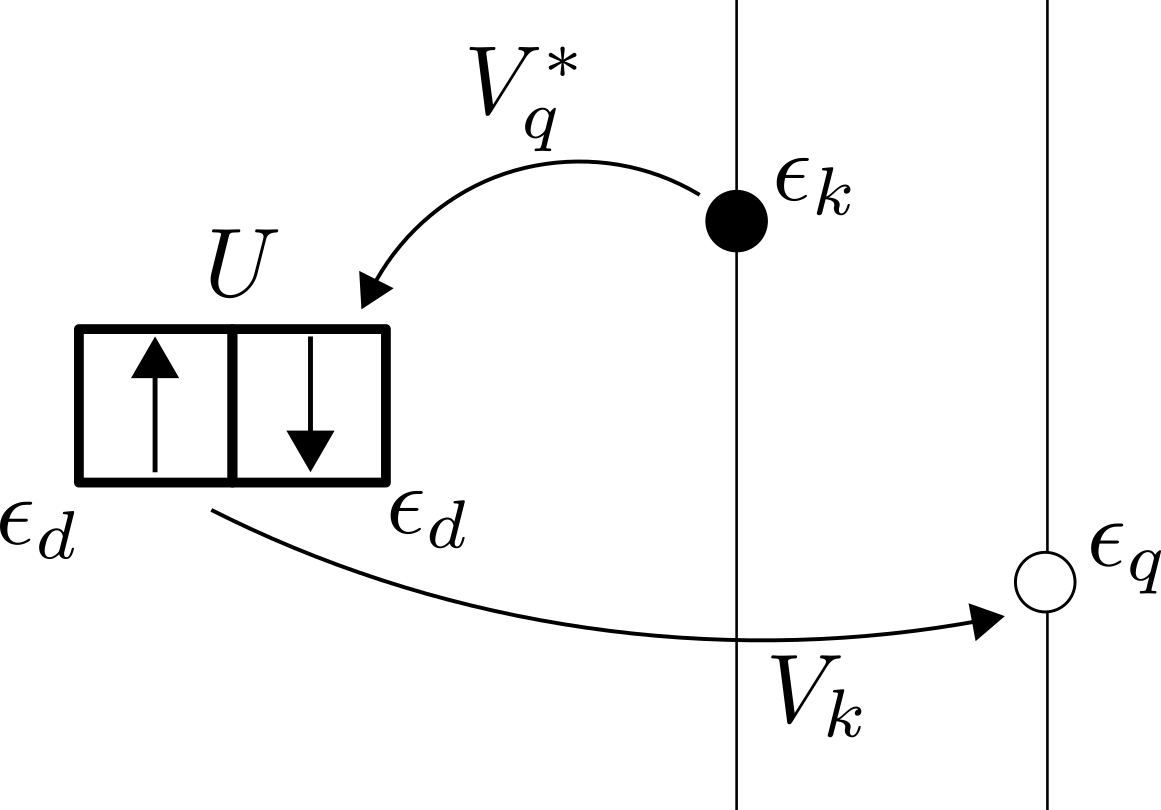
\includegraphics[width=0.5\textwidth]{../figures/model_scheme.png}
	\caption{The single-impurity Anderson model Hamiltonian}
\end{figure}
The SIAM involves the following energy scales:
\begin{itemize}
	\item the onsite energy: \(\epsilon_d\)
	\item the double-occupation cost: \(U\)
	\item the energy scale generated by the hybridisation: \(\Delta = \pi t^2\sum_k \rho(\epsilon_k) \rightarrow \). The rate of hybridisation is \(\frac{2\Delta}{\hbar}\).
\end{itemize}
We can have the following situations regarding dominance of various energy scales:
\begin{itemize}
	\item \(U \gg \epsilon_d \gg \Delta\): Double occupation is not possible.
		\(\Delta\) being small means very small hybridisation.
So, d-site is either up or down, hence magnetic.
    \item \(U \gg \Delta\gg \epsilon_d \): Double occupation is still not possible, but now hybridisation will allows the up and down spins to fluctuate on the d-site, leading to zero average magnetization.
    \item \(\Delta\gg U \gg \epsilon_d\): Hybridisation now fluctuates the up and down spins , leading to zero average magnetization.
\end{itemize}
To get a feel for the dynamic of the model, we can consider the very simple atomic limit (\(V = 0\)).
\begin{equation}\begin{aligned}
H_\text{atomic} = E_d + E_{CB} + U n_{d\uparrow}n_{d\downarrow}
\end{aligned}\end{equation}
Since we are not interested in the Fermi sea and since there is no interaction between that and the impurity, we can choose to look only at the impurity:
\begin{equation}\begin{aligned}
H_\text{atomic} = \epsilon_d n_d + U n_{d\uparrow}n_{d\downarrow}
\end{aligned}\end{equation}
For a magnetic solution, we need
\begin{equation}\begin{aligned}
(\epsilon_\uparrow = \epsilon_\downarrow =)\epsilon_d < (\epsilon_0,\epsilon_{\uparrow\downarrow}) 0,2\epsilon_d + U
\end{aligned}\end{equation}
Assuming \(\epsilon_d = -|\epsilon_d|\), this is equivalent to
\begin{equation}\begin{aligned}
\epsilon_d > -U
\end{aligned}\end{equation}

\subsection{The non-interacting limit}
The non-interacting limit consists of a non-interacting impurity site (\(U = 0\)). This is often referred to as the resonant-level model.
\begin{equation}\begin{aligned}
	H_\text{non-int} = \epsilon_d n_d + \sum_k \epsilon_k n_k + \sum_{k\sigma} t\left(c^\dagger_{k\sigma}c_{d\sigma}+c^\dagger_{d\sigma}c_{k\sigma}\right)
\end{aligned}\end{equation}
\subsubsection{Green's function of impurity site:}
We want to write down the \textit{Green's function} \(G_d\) for the impurity site.
In the absence of the hybridisation, this quantity is
\begin{equation}\begin{aligned}
G^0_d(E) = \frac{1}{E - \epsilon_d}
\end{aligned}\end{equation}
In the presence of the coupling with the conduction band, there are several ways of creating an excitation at the impurity site, with an energy \(E\).
The first is the bare Green's function.
This is the situation when the impurity site electron has not scattered.
Next is the case that there is an excitation with energy E (\(G^0_d(E)\)) followed by a scattering to the conduction band at some momentum \(k\).
The probability of the scattering is \(t\).
The Greens function for creating the electron \(k\) is \(G^0_k = \frac{1}{E-\epsilon_k}\), and the probability of again scattering back to the impurity site is \(t\), with the Greens function for this final excitation being \(G^0_d\).
The total Greens function contribution for this case is
\begin{equation}\begin{aligned}
	G^0_d \Sigma_c G^0_d, \text{  where  }\Sigma_c = t \left(\sum_k G^0_k\right) t = \sum_k \frac{t^2}{E - \epsilon_k}
\end{aligned}\end{equation}
Considering higher scatterings lead to terms like \(G^0_d \Sigma_c G^0_d\Sigma_c G^0_d\),\\\(G^0_d \Sigma_c G^0_d\Sigma_c G^0_d\Sigma_c G^0_d\) and so on.
The total Greens function is
\begin{equation}\begin{aligned}
G_d(E) &= G^0_d + G^0_d \Sigma_c G^0_d + G^0_d \Sigma_c G^0_d\Sigma_c G^0_d + G^0_d \Sigma_c G^0_d\Sigma_c G^0_d\Sigma_c G^0_d + ...
\\
       &= G^0_d\left[1+\left(\Sigma_c G^0_d\right)^2+...\right] = G^0_d \frac{1}{1-\Sigma_c G^0_d} = \frac{1}{E - \epsilon_d - \Sigma_c(E)} 
\end{aligned}\end{equation}
Now,
\begin{gather}
\frac{1}{t^2}\Sigma_c(E) = \sum_k \frac{1}{E - \epsilon_k} = \lim_{\eta \rightarrow 0}\int_{-W}^W d\epsilon \rho(\epsilon) \frac{1}{E - \epsilon + i\eta}\\
\implies \frac{1}{t^2}\text{Re} \left[\Sigma_c(E)\right] = \int_{-W}^W d\epsilon \rho(\epsilon)\frac{1}{E - \epsilon}, \text{and }\\
\frac{1}{t^2}\text{Im} \left[\Sigma_c(E)\right] = \int_{-W}^W d\epsilon \rho(\epsilon) (-i\pi)\delta(E-\epsilon)
\end{gather}
Assuming \(\rho(E)\) varies sufficiently slowly, we can neglect the real part,
\begin{equation}\begin{aligned}
	\Sigma_c(E) = \text{Im}\left[\Sigma_c(E)\right] = -i\pi t^2 \rho(E) = -i\Delta
\end{aligned}\end{equation}
Therefore,
\begin{equation}\begin{aligned}
G_d(E) = \frac{1}{E-\epsilon_d+i\Delta}
\end{aligned}\end{equation}
The difference from \(G^0_d\) can be seen by computing the density of states for both the bare and the interacting ones:
\begin{gather}
	\rho_d^0(E) = -\frac{1}{\pi}\text{Im}\left[G^0_d\right] = -\frac{1}{\pi} \lim_{\eta \rightarrow 0} \frac{1}{E - \epsilon_d + i\eta} = \delta(E - \epsilon_d)\\
	\rho_d(E) = -\frac{1}{\pi}\text{Im}\left[G_d\right]= -\frac{1}{\pi} \lim_{\eta \rightarrow 0} \frac{1}{E - \epsilon_d + i(\eta+\Delta)} = \frac{1}{\pi}\frac{\Delta}{(E-\epsilon_d)^2 + \Delta^2}\label{densitys}
\end{gather}
The first density of states is delta function, because \(\epsilon_d\) is an eigenstate in that case, and the poles of the corresponding Green's function are real poles.
But the presence of the hybridisation means that is no longer the case in the second density of states, so the delta function fades into a Lorentzian in that case, and the poles of the Greens function move off the real axis.
\\\\The total number of d-electrons can be calculated as:
\begin{equation}\begin{aligned}
	\label{total}
	\langle  n_d\rangle = 2\int d\epsilon \rho_d(\epsilon) = \frac{2\Delta}{\pi} \int \frac{d\epsilon}{(\epsilon-\epsilon_d)^2 + \Delta^2} = \frac{2}{\pi}\cot^{-1}\left(\frac{\epsilon_d}{\Delta}\right)
\end{aligned}\end{equation}
\subsubsection{Phase shift of conduction electron due to scattering off the impurity:}
\(T-\)matrix is defined by
\begin{equation}\begin{aligned}
T = V + VGT 
\end{aligned}\end{equation}
We also have
\begin{equation}\begin{aligned}
G = G_0 + G_0VG &= G_0 + G_0 T \frac{1}{1+GT}G \\
        &= G_0 + G_0T(1-GT+...)(G_0+G_0VG_0+...)\\
        &= G_0 + G_0 T G_0 \label{green}
\end{aligned}\end{equation}
The conduction electron Green's function can be calculated as
\begin{equation}\begin{aligned}
G_c(k,k^\prime,E) = \delta_{k,k^\prime}G^0_c(k,E) + G_c^0(k)t G^0_d t G^0_c(k^\prime) + \\ G_c^0(k)t G^0_d t \sum_q G_c^0(q) t G^0_d t G^0_c(k^\prime) + ...\\
\end{aligned}\end{equation}
Noting that 
\begin{equation}\begin{aligned}
t\sum_q G_c^0(q)t = \Sigma_c,
\end{aligned}\end{equation}
we have
\begin{equation}\begin{aligned}
G_c(k,k^\prime,E) = \delta_{k,k^\prime}G^0_c(k,E) + G_c^0(k)t^2 G_d(E)G_c^0(k^\prime)
\end{aligned}\end{equation}
Comparing with the final form of \(G\) in eq.~\ref{green}, we can write
\begin{equation}\begin{aligned}
	\label{tm}
T(k,k^\prime,E) = t^2 G_d(E) = \frac{t^2}{E-\epsilon_d + i\Delta}=-\frac{t^2}{\Delta} \frac{1}{\frac{ \epsilon_d- E}{\Delta}-i}
\end{aligned}\end{equation}
As an aside, this form of the transition matrix allows us to make a connection:
\begin{equation}\begin{aligned}
	\label{dsfromtmat}
	\text{Im}[T] = -\frac{t^2 \Delta}{\left(E-\epsilon_d\right)^2+\Delta^2} = -\pi t^2 \rho_d
\end{aligned}\end{equation}
The density of states of the impurity site is proportional to the imaginary part of the transition matrix element.
This is a general relation, because
\begin{equation}\begin{aligned}
	\rho_d = -\frac{1}{\pi}\text{Im}\left[G_d\right] = -\frac{1}{\pi t^2}\text{Im}\left[t^2 G_d\right] = -\frac{1}{\pi t^2}\text{Im}\left[T\right]
\end{aligned}\end{equation}
This relation will hold as long as the \(T-\)matrix is of the form \(t^2 G_d\).
\\\\
If the phase shift of the conduction electrons due to scattering off the impurity is \(\delta\), we have
\begin{equation}\begin{aligned}
	T = e^{2i\delta} - 1 = e^{i\delta}\left(e^{i\delta} - e^{-i\delta}\right) \sim \frac{1}{\cot \delta - i}
\end{aligned}\end{equation}
Comparing with eq.~\ref{tm}, we can write
\begin{equation}\begin{aligned}
	\label{phaseshift}
	\delta(E) = \cot^{-1}\left(\frac{\epsilon_d - E}{\Delta}\right)
\end{aligned}\end{equation}
When \(E = \epsilon_d\), the phase shift is \(\pi\), and the scattering is head on (the conduction electron is reflected back).
Comparing with eq.~\ref{total},
\begin{equation}\begin{aligned}
	\frac{2}{\pi}\delta(0) = \langle  n_d\rangle
\end{aligned}\end{equation}
This is an example of the Friedel sum rule which states that the total number of electrons bound inside a resonance is \(\frac{1}{\pi}\) times the total scattering phase shift at the Fermi surface.
In other words, the impurity will be singly occupied when \(\delta(0) = \frac{\pi}{2}\).

\subsubsection{Coulomb blockade}
This section follows the discussion in reference \cite{piers}. A quantum dot is a set of electrons that are localized in a sufficiently small region so that their spectrum is quantized.
The localization means that double occupation will come at a cost of \(U\).
\begin{equation}\begin{aligned}
H_\text{dot} = \sum_{m\sigma} \epsilon_m n_{m\sigma} + U\frac{N(N+1)}{2}
\end{aligned}\end{equation}
\(\epsilon_m\) are the single-particle energy levels.
\(N =\sum_{m\sigma} n_{m\sigma}\) is the total number of electrons.
Switching on a voltage \(V\) across the dot shifts the energy levels, creating the possibility of conduction.
\begin{equation}\begin{aligned}
	H_\text{dot} = \sum_{m\sigma} \left(\epsilon_m -eV\right) n_{m\sigma} + U\frac{N(N+1)}{2}
\end{aligned}\end{equation}
\(e\) is positive.
The energy difference between \(n_{N}=1\) and \(n_N = 2\) levels is
\begin{equation}\begin{aligned}
\Delta E = UN + \epsilon_{N} -eV
\end{aligned}\end{equation}
Tuning the voltage can make these two levels degenerate.
\begin{equation}\begin{aligned}
eV^* = UN + \epsilon_{N}
\end{aligned}\end{equation}
At this voltage, the two levels have the same energy and double occupancy becomes possible.
Electrons can flow from the source to the sink via double occupation on the dot.\\\\
For a non-interacting resonance, the conductance can be calculated as follows.
The conductance for perfect transmission is given by the quantum of conductance \(G_0 = \frac{2e^2}{h}\).
In this case, the transmission is not perfect, but is modulated by the density of states of the dot at the Fermi surface.
Hence,
\begin{equation}\begin{aligned}
	G(V) = G_0 \rho(0) = \frac{2e^2}{h} \frac{\Delta^2}{\left(\epsilon_m - eV\right)^2 + \Delta^2}
\end{aligned}\end{equation}
The conductance is maximum whenever \(\epsilon_m = eV\).


\subsection{Total Hamiltonian: Mean field treatment}
\begin{gather}
	n_{d\uparrow}n_{d\downarrow} \approx n_{d\uparrow}\langle  n_{d\downarrow}\rangle + n_{d\downarrow}\langle  n_{d\uparrow}\rangle + \text{constant}\\
	H \approx \sum_k \epsilon_k n_k + \sum_\sigma \left[\epsilon_d+U \langle  n_{d\overline \sigma}\rangle\right]n_{d\sigma} + t\sum_{k\sigma}\left(c^\dagger_{k\sigma}c_{d\sigma}+c^\dagger_{d\sigma}c_{k\sigma}\right)
\end{gather}
The only change is \(\epsilon_d \rightarrow \epsilon_{d\sigma} = \epsilon_d + U\langle  n_{d\bar\sigma}\rangle\).
This allows us to write
\begin{equation}\begin{aligned}
	\label{rho}
	\rho_{d\sigma} = \frac{1}{\pi}\frac{\Delta}{(E-\epsilon_{d\sigma})^2 + \Delta^2} \implies \langle  n_{d\sigma}\rangle = \int \rho_{d\sigma} = \frac{1}{\pi}\cot^{-1}\left(\frac{\epsilon_{d\sigma}}{\Delta}\right)
\end{aligned}\end{equation}
An alternative way of writing that is
\begin{equation}\begin{aligned}
	\label{density}
	\frac{\epsilon_{d\sigma}}{\Delta} = \frac{\epsilon_d + U\langle  n_{d\sigma}\rangle}{\Delta} =  \cot\left(\pi\langle  n_{d\sigma}\rangle\right) \implies \langle  n_{d\sigma}\rangle = \frac{\Delta}{U}\left[{\cot\left(\pi\langle  n_{d\overline\sigma}\rangle\right) - \frac{\epsilon_d}{\Delta}}\right]
\end{aligned}\end{equation}
Introducing \(n_d = \langle  n_{d\uparrow}\rangle + \langle  n_{d\downarrow}\rangle\) and \(m = \langle  n_{d\uparrow}\rangle - \langle  n_{d\downarrow}\rangle\), we can write
\begin{equation}\begin{aligned}
	\langle  n_{d\uparrow} - n_{d\downarrow}\rangle \equiv m = \frac{\Delta}{U}\left[\cot\left(\pi\langle  n_{d\downarrow}\rangle\right)-\cot\left(\pi\langle  n_{d\uparrow}\rangle\right)\right] \\= \frac{\Delta}{U}\left[\cot\frac{\pi}{2}\left(n_d-m\right)-\cot\frac{\pi}{2}\left(n_d+m\right)\right]
\end{aligned}\end{equation}
We want to find the critical condition for the onset of magnetism.
This occurs when \(m \rightarrow 0^+\).
This means we can expand the \(\cot\) around \(m=0\).
Since
\begin{equation}\begin{aligned}
	\cot (a+x) \approx \cot a -x\left(\sin a\right)^{-2} \implies \cot (a-x) - \cot(a+x) \approx 2x\left(\sin a\right)^{-2}
\end{aligned}\end{equation}
we get
\begin{equation}\begin{aligned}
	\label{final}
	m = \frac{\Delta}{U}\left[-\pi\frac{ m}{\sin^2 \frac{\pi}{2} n_d}\right] \implies 1 = \lim_{m \rightarrow 0}\frac{U}{\pi \Delta}\frac{1}{1+\cot^2\frac{\pi n_d}{2}}
\end{aligned}\end{equation}
At \(m=0\), \(\langle  n_{d\uparrow}\rangle = \langle  n_{d\downarrow}\rangle\), therefore \(\cot \frac{\pi n_d}{2} = \frac{U n_d}{2\Delta}+\frac{\epsilon_d}{\Delta}\).
Substituting in eq.~\ref{final},
\begin{equation}\begin{aligned}
	1 = \frac{U_c}{\pi}\frac{\Delta}{\Delta^2+\left(\frac{U_c n_d}{2}+\epsilon_d\right)^2}
\end{aligned}\end{equation}
Magnetism will prevail for \(U \geq U_c\).
Comparing with eq.~\ref{density},
\begin{equation}\begin{aligned}
1 = U_c \rho_d(E=0)
\end{aligned}\end{equation}
At half-filling, \(n_d = 1\) and \(\epsilon_d = -\frac{U}{2}\), which gives
\begin{equation}\begin{aligned}
U_c = \pi \Delta
\end{aligned}\end{equation}
For higher values of \(U\), we get a value of \(m\) far from \(0\).
This provides two peaks in the density of states.
\begin{gather}
	\langle  n_{d\uparrow}\rangle = \frac{1+m}{2}\\
	\langle  n_{d\downarrow}\rangle = \frac{1-m}{2}\\
	\epsilon_{d\sigma} = \epsilon_d + U\langle  n_{d\overline\sigma}\rangle = \epsilon_d + \frac{U}{2} \pm \frac{U}{2}m = \pm \frac{U}{2}m\\
\rho_d = \rho_{d\uparrow} + \rho_{d\downarrow} = \frac{\Delta}{\pi}\left[\frac{1}{\Delta^2 + \left(E - \frac{Um}{2}\right)^2}+\frac{1}{\Delta^2 + \left(E + \frac{Um}{2}\right)^2}\right]
\end{gather}
We get two Lorentzian peaks at \(E = \pm \frac{Um}{2}\), depending on whichever polarization the impurity local moment is in.

\subsection{Some conclusions and observations}
\begin{itemize}
	\item The mean field solution predicts that local moments are sustained in the limit of large \(U\) and small \(|\epsilon_d|\). However, this treatment becomes faulty at low temperatures.
	\item At low temperatures, the resistivity is found to reach a minimum and then vary as \(\ln T\). This behavior stops at some very low temperature \(T_K\). The temperature \(T_K\) is also that at which the magnetization vanishes, and the susceptibility becomes constant, suggesting that the impurity spin has condensed into a singlet.
	\item Since the disappearance of the \(\ln T\) behavior is coincident with the condensation of the spin degree of freedom, it is natural to hope that the resistivity minimum is a result of the interaction between the impurity and the conduction spins.
    \item To describe such an interaction, the way to proceed is to strip the model of the charge excitations (via a \textit{Schrieffer-Wolff transformation}).
The resultant Hamiltonian consists of an anti-ferromagnetic interaction between the itinerant spins and the impurity spin, and is called the Kondo model.
    \item Calculating the scattering rate up to second order using the Kondo model produces a logarithmic term, which explains the log-dependence. Since this perturbative treatment will fail at small temperatures (where the log term diverges), we need some other technique to find out the fate of the model at low temperatures.
    \item Anderson's poor man's scaling wraps the effects of high energy scatterings into the low energy model, showing that the anti-ferromagnetic coupling diverges at low temperatures, producing a singlet.
    \item There are two routes that one can follow to note the changes in the system; one is by reducing the temperature which is equivalent to folding in the high energy fluctuations, aka scaling.
	    The other is to reduce the onsite interaction \(U\) and note the changes in state.
    \item Reducing the temperature or performing the RG takes the model from the Anderson model (\(T>0\)) to the Fermi liquid state (\(T \sim T_K\)).
	    This Fermi liquid may have interactions, depending on the value of \(U\) we are working in.
    \item Coming down to \(T<T_K\), we can now modify the \(U\) from \(\infty\) to 0.
	    Large \(U\) means the Fermi liquid has large interactions.
	    Reducing \(U\) means coming down to a Fermi gas.
	    For \(T\neq 0\), reducing \(U\) means going from local moment regime to non-magnetic regime.
	    For \(T=0\), local moments persist for all \(U>0\).
    \item It will be seen that in the large \(U\) regime, the singlet channel scattering phase shift (phase shift incurred when one singlet state scatters into another singlet state) at the Fermi energy is \(\propto \tan^{-1} J_\text{eff}\).
	    This effective coupling \(J_\text{eff}\) flows to \(\infty\) under poor man's scaling as \(T \rightarrow 0\).
	    Thus, the singlet phase shift at \(\epsilon_F\) approaches \(\frac{\pi}{2}\) as \(T \rightarrow 0\).
\end{itemize}

\section{The Kondo model}
To study the interactions of the spin degrees of freedom, it becomes necessary to integrate out the charge degrees of freedom from the general scattering term \(Vc^\dagger_k c_d + \text{h.c.}\). Doing so produces a simpler Hamiltonian that has the charge fluctuations projected out and only spin fluctuations remaining.
\begin{equation}\begin{aligned}
	H_\text{Kondo} = \sum_{k\sigma}\epsilon_k \hat n_{k\sigma} + \sum_{i=x,y,z} J_i S_d^i s^i
\end{aligned}\end{equation}
\(S_i = \sum_{\alpha \beta} c^\dagger_{d\alpha} \sigma^i_{\alpha\beta} c_{d \beta}\). \(s_i =\sum_{k k^\prime\alpha \beta} c^\dagger_{k\alpha} \sigma^i_{\alpha\beta} c_{k^\prime \beta}\).  Note that the impurity onsite energy has also been dropped because we are in the subspace of constant \(\hat n_d\;(= 1)\). 
\subsection{Derivation of the Kondo Hamiltonian}
Deriving the Kondo Hamiltonian involves separating the impurity spinon subspace (\(\hat n_{d\uparrow} \neq \hat n_{d\downarrow}\)) from the doublon and holon subspaces (\(\hat n_{d\uparrow} = \hat n_{d\downarrow}\)). The canonical (pun intended) way of doing this is via a Schrieffer-Wolff transformation \cite{Schrieffer_Wolff}. It involves applying a unitary transformation on the original Hamiltonian such that the terms that scatter between the two subspaces disappear, up to leading order. We are then left with a higher order intra-subspace scattering. It is often referred to as a one-shot renormalization group method, because it kills all the off-diagonal terms in one iteration. The approach here follows that in \cite{piers}. An alternate derivation via a projector operator method due to \cite{hewson} is shown in \ref{SWT from URG}.
\\\\The space of the impurity electron can be divided into low energy and high energy subspaces:
\begin{equation}\begin{aligned}
\text{low energy (L)} \rightarrow \begin{cases} \ket{\uparrow} \\ \ket{\downarrow} \end{cases}\\
\text{high energy (H)} \rightarrow \begin{cases} \ket{} \\ \ket{\uparrow\downarrow} \end{cases}\\
\end{aligned}\end{equation}
\begin{equation}\begin{aligned}
H = H_0 + V = \bordermatrix{~ & \text{low} & \text{high} \cr 
\text{low} & H^L & v^\dagger \cr
       &&\cr
\text{high} & v & H^H }
\end{aligned}\end{equation}
\begin{equation}\begin{aligned}
	H_0 = \sum_{k}\epsilon_k n_{k}+ \epsilon_d n_d + U n_{d\uparrow}n_{d\downarrow}, V=\sum_{k\sigma}\left(V_k c^\dagger_{k\sigma}c_{d\sigma} +V_k^* c^\dagger_{d\sigma}c_{k\sigma}\right)
\end{aligned}\end{equation}
Let \(S\) be some anti-Hermitian operator, of the order of \(V\).
Expanding in powers of \(V\),
\begin{equation}\begin{aligned}
	\overline H = e^{-S} H e^S = H_0 + \left(V+\left[H_0,S\right]\right) + \frac{1}{2}\left(\left[V,S\right]+\left[\left[H_0,S\right],S\right]\right)
\end{aligned}\end{equation}
Defining \(S\) such that the first order term vanishes,
\begin{gather}
	V = \left[S,H_0\right] \label{sdef}\\
	\overline H = H_0 + \frac{1}{2}\left[V,S\right]
\end{gather}
Take \(S = \begin{pmatrix} 0 & -s^\dagger \\ s & 0 \end{pmatrix}\).
From eq.~\ref{sdef},
\begin{equation}\begin{aligned}
V = \begin{pmatrix} 0 & -s^\dagger \\ s & 0 \end{pmatrix} \begin{pmatrix} H^L & 0 \\ 0 & H^H \end{pmatrix} - \begin{pmatrix} H^L & 0 \\ 0 & H^H \end{pmatrix} \begin{pmatrix} 0 & -s^\dagger \\ s & 0 \end{pmatrix} \\= \begin{pmatrix} 0 & -s^\dagger H^H+H^L s^\dagger \\ s H^L - H^H s & 0 \end{pmatrix}
\end{aligned}\end{equation} 
Comparing with the definition of \(V\), we can write
\begin{gather}
	v^\dagger_{ij} = s^\dagger_{ij}\left(E^L_i - E^H_j\right), v_{ij} = s_{ij}\left(E^L_j - E^H_i\right)\\
\implies s^\dagger_{ij} = \frac{v^\dagger_{ij}}{E^L_i - E^H_j}, s_{ij} = \frac{v_{ij}}{E^L_j - E^H_i}
\end{gather}
From the structure of \(S\), it is clear that \(i \in H, j \in L\).
\begin{equation}\begin{aligned}
	\left[V,S\right] = \begin{pmatrix} 0 & v^\dagger \\ v & 0 \end{pmatrix}\begin{pmatrix} 0 & -s^\dagger \\ s & 0 \end{pmatrix} - \begin{pmatrix} 0 & -s^\dagger \\ s & 0 \end{pmatrix}\begin{pmatrix} 0 & v^\dagger \\ v & 0 \end{pmatrix} = \begin{pmatrix} v^\dagger s + s^\dagger v & 0 \\ 0 & -vs^\dagger -sv^\dagger \end{pmatrix}
\end{aligned}\end{equation}
Hence,
\begin{equation}\begin{aligned}
	\overline H = H_0 + \frac{\left[V,S\right]}{2} = \begin{pmatrix} H^L + \frac{1}{2}\left(v^\dagger s + s^\dagger v\right) & 0 \\ 0 & H^H -vs^\dagger -sv^\dagger \end{pmatrix}
\end{aligned}\end{equation}
Since we want the low energy excitations, the effective low-energy Hamiltonian is
\begin{equation}\begin{aligned}
	\mathcal{H} = \bra{L} \overline H \ket{L} = H^L + \frac{1}{2}\left(v^\dagger s + s^\dagger v\right)
\end{aligned}\end{equation}
where \(H^L = \sum_\sigma \bra{\sigma_d} H_0 \ket{\sigma_d} = \epsilon_d n_d + \sum_{k} n_{k}\).
Now,
\begin{equation}\begin{aligned}
	\Delta H = \frac{1}{2}\left(v^\dagger s + s^\dagger v\right) &= \frac{1}{2}\left(v^\dagger \sum_{HL} s_{HL}\ket{H}\bra{L} + \text{h.c.}\right) \\
								     &= \frac{1}{2}\sum_{HL}\left[v^\dagger \ket{H}\bra{L}\frac{v_{HL}}{E_L - E_H} + \ket{L}\bra{H} \frac{v^\dagger_{LH}}{E_L - E_H}v\right]
\end{aligned}\end{equation}
Taking a matrix element between two low energy states \(l, l^\prime\), we get
\begin{equation}\begin{aligned}
	\Delta H_{ll^\prime} = \bra{l} \Delta H \ket{l^\prime} &= \frac{1}{2}\sum_H v^\dagger_{lH}v_{Hl^\prime}\left(\frac{1}{E_{l^\prime} - E_H}+\frac{1}{E_l - E_H}\right)
\end{aligned}\end{equation}
This can also be written as
\begin{equation}\begin{aligned}
	\label{hamtmat}
	\Delta H_{ll^\prime} = \frac{1}{2}\left[T_{ll^\prime}(E_l) + T_{ll^\prime}(E_{l^\prime})\right]
\end{aligned}\end{equation}
where 
\begin{equation}\begin{aligned}
T_{ll^\prime}(E) = \sum_H \frac{v^\dagger_{lH}v_{Hl^\prime}}{E-E_H} = \sum_H \frac{V^\dagger_{lH} V_{Hl^\prime}}{E-E_H}
\end{aligned}\end{equation}
\(T(E)\), here, is the second order contribution of the \(T-\)matrix due to scattering off the interaction \(V\).
The \(\ket{H}\) act as the intermediate states during the second order scatterings.
This is a slight generalization from second order perturbation theory.
In second order perturbation, we only consider the scattering amplitude between the same states, but here we consider the scattering between two potentially different states \(\ket{l},\ket{l^\prime}\).
The total amplitude is an average of these two amplitudes.
\\\\If we assume the high energy subspace is very far away from the low energy one (\(E_H \gg E_L\)), we can assume \(E_l \approx E_{l^\prime} = E_L\), we can write
\begin{equation}\begin{aligned}
\Delta H_{ll^\prime} &=\sum_H v^\dagger_{lH}v_{Hl^\prime}\frac{1}{E_L-E_H}\\
\implies \Delta H &=V \left(\sum_H \frac{1}{\Delta_{LH}}\ket{H}\bra{H}\right)V
\end{aligned}\end{equation}
where \(\Delta_{LH}=E_L - E_H\) is the energy difference between the low energy subspace and the high energy state \(\ket{H}\).
For our Hamiltonian, \(\ket{H_1} = \ket{0}, \ket{H_2} = \ket{\uparrow\downarrow}\).
Therefore,
\begin{equation}\begin{aligned}
	\Delta_{LH_1} = \epsilon_d - 0 = \epsilon_d, \Delta_{LH_2} = \epsilon_d - \left(2\epsilon_d + U\right) = -\epsilon_d - U
\end{aligned}\end{equation}
Also, \(V = \sum_{k\sigma}\left[V(k) c^\dagger_{k\sigma}c_{d\sigma} + V^*(k) c^\dagger_{d\sigma}c_{k\sigma}\right]\).
Hence,
\begin{equation}\begin{aligned}
\Delta H &= V\frac{\ket{0}\bra{0}}{\epsilon_d}V - V\frac{\ket{\uparrow\downarrow}\bra{\uparrow\downarrow}}{\epsilon_d + U}V\\
	 &= \sum_{k_1,k_2,\sigma_1,\sigma_2}V(k_1)V^*(k_2)\left[\frac{c^\dagger_{d\sigma_2} c_{k_2 \sigma_2}\ket{0}\bra{0}c^\dagger_{k_1\sigma_1} c_{d \sigma_1}}{\epsilon_d} - \frac{c^\dagger_{k_1\sigma_1} c_{d \sigma_1}\ket{\uparrow\downarrow}\bra{\uparrow\downarrow}c^\dagger_{d\sigma_2} c_{k_2 \sigma_2}}{\epsilon_d+U}\right]\\
&=\sum_{k_1,k_2,\sigma_1,\sigma_2}V(k_1)V^*(k_2)\frac{c^\dagger_{d\sigma_2} c_{k_2 \sigma_2}c^\dagger_{k_1\sigma_1} c_{d \sigma_1}\ket{d\sigma_1,h_{k_1\sigma_1}}\bra{d\sigma_1,h_{k_1\sigma_1}}}{\epsilon_d} \\
&- \sum_{k_1,k_2,\sigma_1,\sigma_2}V(k_1)V^*(k_2)\frac{c^\dagger_{k_1\sigma_1} c_{d \sigma_1}c^\dagger_{d\sigma_2} c_{k_2 \sigma_2}\ket{d\overline{\sigma_2},e_{k_2\sigma_2}}\bra{d\overline{\sigma_2},e_{k_2\sigma_2}}}{\epsilon_d+U}\\
&=\sum_{k_1,k_2,\sigma_1,\sigma_2}V(k_1)V^*(k_2)\left[\frac{c^\dagger_{d\sigma_2} c_{k_2 \sigma_2}c^\dagger_{k_1\sigma_1} c_{d \sigma_1}}{\epsilon_d} - \frac{c^\dagger_{k_1\sigma_1} c_{d \sigma_1}c^\dagger_{d\sigma_2} c_{k_2 \sigma_2}}{\epsilon_d+U}\right]P_{n_d=1}
\end{aligned}\end{equation}
Using the Fierz identity \(\delta_{\sigma_1\sigma_3}\delta_{\sigma_4\sigma_2} = \frac{1}{2}\delta_{\sigma_1\sigma_2}\delta_{\sigma_3\sigma_4} + \frac{1}{2}\vec\sigma_{\sigma_1\sigma_2}\cdot\vec\sigma_{\sigma_3\sigma_4}\), we can write
\begin{equation}\begin{aligned}
c^\dagger_{d\sigma_2} c_{k_2 \sigma_2}c^\dagger_{k_1\sigma_1} c_{d \sigma_1} &= \sum_{\sigma_3,\sigma_4}c^\dagger_{d\sigma_3} c_{k_2 \sigma_2}c^\dagger_{k_1\sigma_1} c_{d \sigma_4}\delta_{\sigma_1\sigma_3}\delta_{\sigma_4\sigma_2}\\
									     &=\frac{1}{2}\sum_{\sigma_3,\sigma_4}c^\dagger_{d\sigma_3} c_{k_2 \sigma_2}c^\dagger_{k_1\sigma_1} c_{d \sigma_4}\left(\delta_{\sigma_1\sigma_2}\delta_{\sigma_3\sigma_4} + \vec\sigma_{\sigma_1\sigma_2}\cdot\vec\sigma_{\sigma_3\sigma_4}\right)\\
&=\frac{1}{2} c_{k_2 \sigma_1}c^\dagger_{k_1\sigma_1}n_d+c_{k_2 \sigma_2}c^\dagger_{k_1\sigma_1}\vec\sigma_{\sigma_1\sigma_2}\cdot\sum_{\sigma_3,\sigma_4}c^\dagger_{d\sigma_3}\frac{\vec \sigma_{\sigma_3\sigma_4}}{2}c_{d\sigma_4}
\end{aligned}\end{equation}
Now, \(c_{k_2 \sigma_1}c^\dagger_{k_1\sigma_1} = \delta_{k_1,k_2}-c^\dagger_{k_1\sigma_1}c_{k_2 \sigma_1}\), and  \(c_{k_2 \sigma_2}c^\dagger_{k_1\sigma_1} = \delta_{\sigma_1,\sigma_2}\delta_{k_1,k_2}-c^\dagger_{k_1\sigma_1}c_{k_2 \sigma_1}\).
The \(\delta\) will result in terms that have no interaction, so we drop these terms.
Also, the \(P_{n_d=1}\) ensures we can substitute \(n_d=1\).
\begin{equation}\begin{aligned}
c^\dagger_{d\sigma_2} c_{k_2 \sigma_2}c^\dagger_{k_1\sigma_1} c_{d \sigma_1} &= -\frac{1}{2} c^\dagger_{k_1\sigma_1}c_{k_2 \sigma_1} - c^\dagger_{k_1\sigma_1}\vec\sigma_{\sigma_1\sigma_2}c_{k_2 \sigma_2}\cdot\sum_{\sigma_3,\sigma_4}c^\dagger_{d\sigma_3}\frac{\vec\sigma_{\sigma_3\sigma_4}}{2}c_{d\sigma_4}\\
\end{aligned}\end{equation}
Since the first term does not have any spin-spin interaction, we drop that term.

Defining \(\vec \sigma_d = \sum_{\sigma_3,\sigma_4}c^\dagger_{d\sigma_3}\vec\sigma_{\sigma_3\sigma_4}c_{d\sigma_4}\), we have
\begin{equation}\begin{aligned}
c^\dagger_{d\sigma_2} c_{k_2 \sigma_2}c^\dagger_{k_1\sigma_1} c_{d \sigma_1} =-\frac{1}{2} c^\dagger_{k_1\sigma_1}\vec\sigma_{\sigma_1\sigma_2}c_{k_2 \sigma_2}\cdot \vec \sigma_d
\end{aligned}\end{equation}
Similarly,
\begin{equation}\begin{aligned}
c^\dagger_{k_1\sigma_1} c_{d \sigma_1} c^\dagger_{d\sigma_2} c_{k_2 \sigma_2}=-\frac{1}{2} c^\dagger_{k_1\sigma_1}\vec\sigma_{\sigma_1\sigma_2}c_{k_2 \sigma_2}\cdot \vec \sigma_d
\end{aligned}\end{equation}
Finally, putting all this together,
\begin{equation}\begin{aligned}
	\Delta H = \frac{1}{2}\sum_{k_1,k_2,\sigma_1,\sigma_2}V(k_1)V^*(k_2)\left[\frac{1}{\epsilon_d+U}-\frac{1}{\epsilon_d}\right]c^\dagger_{k_1\sigma_1}\vec\sigma_{\sigma_1\sigma_2}c_{k_2 \sigma_2}\cdot \vec \sigma_d \\
= \frac{1}{2}\sum_{k_1,k_2,\sigma_1,\sigma_2} J(k_1,k_2)c^\dagger_{k_1\sigma_1}\vec\sigma_{\sigma_1\sigma_2}c_{k_2 \sigma_2}\cdot \vec \sigma_d
\end{aligned}\end{equation}
where
\begin{equation}\begin{aligned}
	\label{jexpr}
	J(k_1,k_2) = V(k_1)V^*(k_2)\left[\frac{1}{\epsilon_d+U}-\frac{1}{\epsilon_d}\right]
\end{aligned}\end{equation}
Assuming \(V(k) \equiv t\),
\begin{equation}\begin{aligned}
H_K = \sum_k \epsilon_k n_k + \frac{J}{2} \vec \sigma_e \cdot \vec \sigma_d
\end{aligned}\end{equation}
where
\begin{equation}\begin{aligned}
\vec \sigma_e = \sum_{k_1,k_2,\sigma_1,\sigma_2}c^\dagger_{k_1\sigma_1}\vec\sigma_{\sigma_1\sigma_2}c_{k_2 \sigma_2} = \sum_{\sigma_1,\sigma_2}c^\dagger_{\sigma_1}(\vec r = 0)\vec\sigma_{\sigma_1\sigma_2}c_{\sigma_2}(\vec r = 0)
\end{aligned}\end{equation}
\(\vec \sigma_e\) is thus the spin density at the origin.

\subsection{Obtaining the resistivity minimum and \(\log\)-dependence}
The next few sections follow the approach in \cite{phill}. The model we are working with is
\begin{equation}\begin{aligned}
H_K &= H_0 + V = \sum_k \epsilon_k n_k + \frac{J}{2} \sum_{k_1,k_2,\sigma_1,\sigma_2}c^\dagger_{k_1\sigma_1}\vec \sigma_d \cdot \vec\sigma_{\sigma_1\sigma_2}c_{k_2 \sigma_2}
\end{aligned}\end{equation}
\begin{equation}\begin{aligned}
	\sum_{\sigma_1,\sigma_2}c^\dagger_{k_1\sigma_1}\vec \sigma_d \cdot \vec\sigma_{\sigma_1\sigma_2}c_{k_2 \sigma_2} = \sigma_d^z\left(c^\dagger_{k_1\uparrow}c_{k_2\uparrow} - c^\dagger_{k_1\downarrow}c_{k_2\downarrow}\right) +\sigma_d^x\left(c^\dagger_{k_1\downarrow}c_{k_2\uparrow} + c^\dagger_{k_1\uparrow}c_{k_2\downarrow}\right) \\
	-i \sigma_d^y\left( c^\dagger_{k_1\uparrow}c_{k_2\downarrow}- c^\dagger_{k_1\downarrow}c_{k_2\uparrow}\right)
\end{aligned}\end{equation}
\begin{equation}\begin{aligned}
	=\sigma_d^z\left(c^\dagger_{k_1\uparrow}c_{k_2\uparrow} - c^\dagger_{k_1\downarrow}c_{k_2\downarrow}\right) + c^\dagger_{k_1\downarrow}c_{k_2\uparrow}\sigma_d^+ + c^\dagger_{k_1\uparrow}c_{k_2\downarrow}\sigma_d^-
\end{aligned}\end{equation}
where \(\sigma^\pm = \sigma^x \pm i \sigma^y\).
Therefore,
\begin{equation}\begin{aligned}
	H_K &=\sum_k \epsilon_k n_k + \frac{J}{2} \sum_{k_1,k_2}\left[\sigma_d^z\left(c^\dagger_{k_1\uparrow}c_{k_2\uparrow} - c^\dagger_{k_1\downarrow}c_{k_2\downarrow}\right)+\sigma_d^+ c^\dagger_{k_1\downarrow}c_{k_2\uparrow} + \sigma_d^- c^\dagger_{k_1\uparrow}c_{k_2\downarrow}\right]\\
	    &=\sum_k \epsilon_k n_k + J \sum_{k_1,k_2}\left[S_d^z\left(c^\dagger_{k_1\uparrow}c_{k_2\uparrow} - c^\dagger_{k_1\downarrow}c_{k_2\downarrow}\right)+S_d^+ c^\dagger_{k_1\downarrow}c_{k_2\uparrow} + S_d^- c^\dagger_{k_1\uparrow}c_{k_2\downarrow}\right]
\end{aligned}\end{equation}
To see the \(\log-\)dependence, we need to calculate the transition matrix up to second order:
\begin{equation}\begin{aligned}
T = V + V G_0 V
\end{aligned}\end{equation}
We wish to calculate the scattering probability of a conduction electron \(\ket{k \uparrow}\).
\subsubsection{First order scattering}
\begin{center}
$\left.\begin{tabular}{@{}l@{}}
		\(\ket{k \uparrow, d_\sigma} \rightarrow \ket{q \uparrow, d_\sigma}\)
		%\(\ket{k \downarrow, d_\sigma} \rightarrow \ket{q \downarrow, d_\sigma}\)\\
\end{tabular}\right\}$ non-spin-flip\\[10pt]
$\left.\begin{tabular}{@{}l@{}}
		\(\ket{k \uparrow, d_\downarrow} \rightarrow \ket{q \downarrow, d_\uparrow}\)
		%\(\ket{k \downarrow, d_\uparrow} \rightarrow \ket{q \uparrow, d_\downarrow}\)\\
\end{tabular}\right\}$ pro-spin-flip
\end{center}
For non-flip, the matrix elements for the \(T-\)matrix is
\begin{equation}\begin{aligned}
T^{(1)}_\text{non-flip} = T_{k_\uparrow,d_{\sigma} \rightarrow q_\uparrow,d_{\sigma}} = \bra{q_\uparrow,d_{\sigma}}V\ket{k_\uparrow,d_{\sigma}} = m_d J
\end{aligned}\end{equation}
where \(m_d \in \{-s_d, s_d\}\) is the spin of the impurity electron.
The probability for this scattering is
\begin{equation}\begin{aligned}
\mathcal{P}_{k_\sigma,d_{\sigma^\prime} \rightarrow q_\sigma,d_{\sigma^\prime}} = 2\pi\sum_{\epsilon} \rho(\epsilon)T_{k_\uparrow,d_{\sigma} \rightarrow q_\uparrow,d_{\sigma}}^2 = 2\pi \rho(0) J^2 m_d^2
\end{aligned}\end{equation}
Since we are considering scattering close to the Fermi surface, we replaced the sum with \(\rho(0)\).

\begin{equation}\begin{aligned}
\mathcal{P}_1 = 2\pi\rho(0)J^2 m_d^2
\end{aligned}\end{equation}
For spin-flip, the matrix element is
\begin{equation}\begin{aligned}
T^{(1)}_\text{flip} =T_{k_\uparrow,d_{\downarrow} \rightarrow q_\downarrow,d_{\uparrow}} = \bra{q_\downarrow,d_{\uparrow}}V\ket{k_\uparrow,d_{\downarrow}} = \lambda_+ J
\end{aligned}\end{equation}
where \(\lambda_\pm = \bra{m_d \pm 1} S_d^\pm \ket{m_d} = \sqrt{s_d(s_d+1)-m_d(m_d\pm 1)}\).
The probability for this scattering is hence
\begin{equation}\begin{aligned}
	\mathcal{P}_2 = \mathcal{P}_{k_\uparrow,d_{\downarrow} \rightarrow q_\downarrow,d_{\uparrow}} = 2\pi \rho(0) J \left[s_d(s_d+1)-m_d(m_d + 1)\right]
\end{aligned}\end{equation}
The total first order scattering probability is (averaged over all configurations of the impurity)
\begin{equation}\begin{aligned}
	\mathcal{P}^{(1)} = \frac{1}{2s_d+1}\sum_{m_d = -s_d}^{s_d}\left(\mathcal{P}_1 + \mathcal{P}_2\right) = \frac{2\pi \rho(0) J^2}{(2s_d+1)}\sum_{m_d = -s_d}^{s_d}\left(s_d(s_d+1) - m_d\right) \\
= 2\pi \rho(0)J^2 s_d(s_d+1)
\end{aligned}\end{equation}
\subsubsection{Second order scattering}

\begin{center}
$\left.\begin{tabular}{@{}l@{}}
		\text{no-impurity-flip}\(\begin{cases}
\ket{k \uparrow, d_\sigma} \rightarrow \ket{q \uparrow, d_\sigma} \rightarrow \ket{k^\prime \uparrow, d_\sigma}\\
\ket{k \uparrow, q \uparrow, d_\sigma} \rightarrow \ket{k \uparrow, k^\prime \uparrow, d_\sigma} \rightarrow \ket{k^\prime \uparrow,q \uparrow, d_\sigma}
\end{cases}\)\\[30pt]
\text{pro-impurity-flip}\(\begin{cases} 
\ket{k \uparrow, d_\downarrow} \rightarrow \ket{q \downarrow, d_\uparrow} \rightarrow \ket{k^\prime \uparrow, d_\downarrow}\\
\ket{k \uparrow, q \downarrow, d_\uparrow} \rightarrow \ket{k \uparrow, k^\prime \uparrow, d_\downarrow} \rightarrow \ket{k^\prime \uparrow,q \downarrow, d_\uparrow}
\end{cases}\)
\end{tabular}\right\}$ no-cond-flip\\[40pt]
$\left.\begin{tabular}{@{}l@{}}
		\text{flip-first}\(\begin{cases} 
\ket{k \uparrow, d_\downarrow} \rightarrow \ket{q \downarrow, d_\uparrow} \rightarrow \ket{k^\prime \downarrow, d_\uparrow}\\
\ket{k \uparrow, q \uparrow, d_\downarrow} \rightarrow \ket{k \uparrow, k^\prime \downarrow, d_\uparrow} \rightarrow \ket{k^\prime \downarrow,q \uparrow, d_\uparrow}
\end{cases}\)\\[30pt]
\text{flip-later}\(\begin{cases} 
\ket{k \uparrow, d_\downarrow} \rightarrow \ket{q \uparrow, d_\downarrow} \rightarrow \ket{k^\prime \downarrow, d_\uparrow}\\
\ket{k \uparrow, q \downarrow, d_\downarrow} \rightarrow \ket{k \uparrow, k^\prime \downarrow, d_\downarrow} \rightarrow \ket{k^\prime \downarrow,q \downarrow, d_\uparrow}
\end{cases}\)\\
\end{tabular}\right\}$ pro-cond-flip
\end{center}
The second order transition matrix contribution is of the form
\begin{equation}\begin{aligned}
T^{(2)}_{i \rightarrow j} = \bra{j} V G_0 V \ket{i} = \sum_l \frac{\bra{j}V\ket{l}\bra{l}V\ket{i}}{E_i - E_l}
\end{aligned}\end{equation}
The sum is over all the intermediate states in going from \(\ket{i}\) to \(\ket{k}\).
For no flipping of the conduction electron, there are four possible processes.
The first process has the following \textit{T}-matrix:
\begin{equation}\begin{aligned}
T^{(2)}_{11}&=\sum_q\frac{\bra{k^\prime_\uparrow d_\sigma}V\ket{q_\uparrow d_\sigma}\bra{q_\uparrow d_\sigma}V\ket{k_\uparrow d_\sigma}}{\epsilon_k-\epsilon_q}\\
	    &= \left(J m_d\right)^2\sum_q \frac{1-P(q)}{\epsilon_k - \epsilon_q} = J^2 m_d^2 \sum_q \frac{1-P(q)}{\epsilon_k - \epsilon_q}
\end{aligned}\end{equation}
where \(m_d = \bra{d_\sigma}S_d^z\ket{d_\sigma}\) and \(1-P(q)\) is the probability that the state \(q\uparrow\) is empty.
For the second process,
\begin{equation}\begin{aligned}
T^{(2)}_{12} = \sum_q \frac{\bra{q_\uparrow k^\prime_\uparrow d_\sigma} V \ket{k^\prime_\uparrow k_\uparrow d_\sigma}\bra{k^\prime_\uparrow k_\uparrow d_\sigma}V\ket{q_\uparrow k_\uparrow d_\sigma}}{\epsilon_q - \epsilon_{k^\prime}}P(q)
\end{aligned}\end{equation}
Note that if \(\bra{k^\prime k}V\ket{q k} \sim \bra{k^\prime k} c^\dagger_{k^\prime}c_q\ket{q k} = 1\), then \(\bra{q k^\prime }V\ket{k^\prime k} \sim \bra{qk^\prime }c^\dagger_q c_k\ket{k^\prime k} =\)\\\( -\bra{qk^\prime }c^\dagger_q c_k\ket{k k^\prime} = -1\).
Assuming the scattering conserves energy \((\epsilon_k = \epsilon_k^\prime)\), we get
\begin{equation}\begin{aligned}
T^{(2)}_{12} = -J^2 m_d^2\sum_q\frac{P(q)}{\epsilon_q - \epsilon_{k}} = J^2 m_d^2 \sum_q \frac{P(q)}{\epsilon_k - \epsilon_q}
\end{aligned}\end{equation}
For the third process,
\begin{equation}\begin{aligned}
T^{(2)}_{13}=\sum_q\frac{\bra{k^\prime_\uparrow d_\downarrow}V\ket{q_\downarrow d_\uparrow}\bra{q_\downarrow d_\uparrow}V\ket{k_\uparrow d_\downarrow}}{\epsilon_k-\epsilon_q}
\end{aligned}\end{equation}
Using \(\bra{m_d\pm 1}S_d^\pm\ket{m_d} = \sqrt{s_d(s_d+1)-m_d(m_d\pm 1)} = \lambda_\pm\), we get
\begin{equation}\begin{aligned}
T^{(2)}_{13} = \lambda_+^2J^2 \sum_q \frac{1-P(q)}{\epsilon_k-\epsilon_q}
\end{aligned}\end{equation}
For the fourth process,
\begin{equation}\begin{aligned}
T^{(2)}_{14}&=\sum_q\frac{\bra{q_\downarrow k^\prime_\uparrow d_\uparrow}V\ket{k^\prime_\uparrow k_\uparrow d_\downarrow}\bra{k^\prime_\uparrow k_\uparrow d_\downarrow}V\ket{q_\downarrow k_\uparrow d_\uparrow}}{\epsilon_q-\epsilon_k^\prime}\\
      &=-\lambda_-^2J^2 \sum_q \frac{P(q)}{\epsilon_q-\epsilon_k}\\
      &=\lambda_-^2J^2 \sum_q \frac{P(q)}{\epsilon_k-\epsilon_q}
\end{aligned}\end{equation}
The sum of all the elements gives the transition matrix element for the scattering \(k\uparrow \rightarrow k^\prime\uparrow\):
\begin{equation}\begin{aligned}
	T^{(2)}_{\text{nonflip}} = \sum_{i=1}^4 T^{(2)}_{1i} &= J^2 \sum_q \frac{m_d^2 + \lambda_+^2 -P(q)\left(\lambda_+^2 - \lambda_-^2\right)}{\epsilon_k-\epsilon_q}\\
&= J^2 \sum_q \frac{s(s+1)-m_d + 2m_dP(q)}{\epsilon_k-\epsilon_q}\\
&= J^2\left[s(s+1)-m_d\right] (\alpha+\gamma) + 2 J^2 m_d \gamma
\end{aligned}\end{equation}
where \(\gamma = \sum_q\frac{P(q)}{\epsilon_k-\epsilon_q},\alpha = \sum_q\frac{1-P_q}{\epsilon_k- \epsilon_q}\).
The second term has the Fermi-Dirac distribution and hence is the only temperature dependent term.
Accordingly, we drop the first term.
\begin{equation}\begin{aligned}
T^{(2)}_{\text{nonflip}} &= 2 J^2 m_d \gamma\\
             &=2J^2 m_d \int d\epsilon N(\epsilon) \frac{P(\epsilon)}{\epsilon_k - \epsilon} = \frac{\sqrt 2 J^2 m_d m^{\frac{3}{2}}}{\pi^2 \hbar^3}\int d\epsilon \frac{\sqrt \epsilon P(\epsilon)}{\epsilon_k - \epsilon}
\end{aligned}\end{equation}
Assuming \(T=0\), \(P(\epsilon) = \theta(\epsilon_F - \epsilon)\).
Then
\begin{equation}\begin{aligned}
T^{(2)}_{\text{nonflip}} &=\frac{\sqrt 2 J^2 m_d m^{\frac{3}{2}}}{\pi^2 \hbar^3}\sqrt{\epsilon_k}\ln \bigg\vert \frac{\sqrt{\epsilon_k}+\sqrt{\epsilon_{F}}}{\sqrt {\epsilon_k}-\sqrt{\epsilon_{F}}} \bigg\vert \\
    &= \frac{\sqrt 2 J^2 m_d m^{\frac{3}{2}}}{\pi^2 \hbar^3}\sqrt{\epsilon_k} \ln \bigg\vert \frac{\epsilon_k + \epsilon_{F} + 2\sqrt{\epsilon_k \epsilon_F}}{\epsilon_k-\epsilon_{F}} \bigg\vert 
\end{aligned}\end{equation}
For \(T >0\) but \(\ll T_F\), the excitation energy of the electrons is very small and of the order of \(k_B T\).
Hence, we can replace \(\epsilon_k - \epsilon_F = k_B T\) and everywhere else replace \(\epsilon_k = \epsilon_F\).

\begin{equation}\begin{aligned}
T^{(2)}_{\text{nonflip}} = \frac{\sqrt 2 J^2 m_d m^{\frac{3}{2}}}{\pi^2 \hbar^3}\sqrt{\epsilon_F} \ln \bigg\vert \frac{4T_F}{T} \bigg\vert 
\end{aligned}\end{equation}
Dropping the temperature-independent \(\log 4\) term and recognizing \(N(\epsilon_F)\) in the pre-factor,
\begin{equation}\begin{aligned}
T^{(2)}_{\text{nonflip}} = 2J^2 m_d N(\epsilon_F) \ln \bigg\vert \frac{T_F}{T} \bigg\vert 
\end{aligned}\end{equation}
Adding the first order non-flip contribution (\(T^{(1)}_\text{nonflip}\)) to the \(T-\)matrix, we get
\begin{equation}\begin{aligned}
	T_\text{nonflip} = J m_d\left[1+2N(\epsilon_F) J \ln \frac{T_F}{T}\right]
\end{aligned}\end{equation}
The upshot is that the additional contribution in second order is obtained by replacing \(J \rightarrow 2J N(\epsilon_F) \ln \frac{T_F}{T}\).
For the spin-flip scatterings (processes 5\textsuperscript{th} to 8\textsuperscript{th}),
\begin{equation}\begin{aligned}
T^{(2)}_{21} &= -J^2 (m_d+1)\lambda_+\sum_q\frac{1-P_q}{\epsilon_k- \epsilon_q}\\
T^{(2)}_{23} &= J^2 m_d \lambda_+\sum_q\frac{1-P_q}{\epsilon_k- \epsilon_q}\\
T^{(2)}_{22} &= J^2 (m_d+1) \lambda_+  \sum_q \frac{P(q)}{\epsilon_k - \epsilon_q}\\
T^{(2)}_{24} &= -\lambda_+ m_d J^2 \sum_q \frac{P(q)}{\epsilon_k-\epsilon_q}
\end{aligned}\end{equation}
\begin{equation}\begin{aligned}
	T^{(2)}_\text{flip} = -J^2 \lambda_+ \left(\alpha - \gamma\right)
\end{aligned}\end{equation}
The total spin-flip matrix element (temperature-dependent part) is
\begin{equation}\begin{aligned}
T^{(2)}_\text{flip} &= 2 J^2 \lambda_+ \sum_q \frac{P(q)}{\epsilon_k - \epsilon_q} \\
     &= 2 J^2 \lambda_+ N(\epsilon_F) \ln \bigg\vert \frac{T_F}{T} \bigg\vert 
\end{aligned}\end{equation}
Adding the first order contribution,
\begin{equation}\begin{aligned}
	T_\text{flip} = \lambda_+ J \left[1 + 2 N(\epsilon_F) J \ln \frac{T}{T_F}\right]
\end{aligned}\end{equation}
Here again, the second order contribution is obtained by replacing \\
\(J \rightarrow 2J N(\epsilon_F) \ln \frac{T_F}{T}\).
Both the solutions together imply that the next order probability for scattering of \(k\uparrow\) is obtained by replacing the additional \(J\) with \(2J N(\epsilon_F) \ln \frac{T_F}{T}\).
\begin{equation}\begin{aligned}
	\label{change1}
	\mathcal{P} = \mathcal{P}^{(2)}\left[1 + 2J N(\epsilon_F) \ln \frac{T_F}{T}\right]
\end{aligned}\end{equation}

\subsection{The Kondo resonance}
Since \(V\) conserves total angular momentum, \(\bra{s}V\ket{s^\prime} \sim \delta_{s s^\prime}\).
Hence
\begin{equation}\begin{aligned}
T_{a \rightarrow b} = \sum_{s,m_s} |\langle {s,m_s}|{a}\rangle|^2 T_s
\end{aligned}\end{equation}
Now, \(\ket{k \uparrow, d_\uparrow} = \ket{s=1}\), so
\begin{equation}\begin{aligned}
T_{\ket{k \uparrow, d_\uparrow} \rightarrow \ket{k^\prime \uparrow d_\uparrow}} = T_1
\end{aligned}\end{equation}
But.
since \(\ket{k \uparrow, d_\downarrow} = \frac{\ket{s=1}+\ket{s=0}}{\sqrt 2}\),
\begin{equation}\begin{aligned}
T_{\ket{k \uparrow, d_\downarrow} \rightarrow \ket{k^\prime \uparrow d_\downarrow}} = \frac{T_1 + T_0}{2}
\end{aligned}\end{equation}
and \(\ket{k \downarrow, d_\uparrow} = \frac{\ket{s=1}-\ket{s=0}}{\sqrt 2}\),
\begin{equation}\begin{aligned}
T_{\ket{k \uparrow, d_\downarrow} \rightarrow \ket{k^\prime \downarrow d_\uparrow}} = \frac{T_1 - T_0}{2}
\end{aligned}\end{equation}
Therefore,
\begin{equation}\begin{aligned}
T_1 = T_{\ket{k \uparrow, d_\downarrow} \rightarrow \ket{k^\prime \uparrow d_\downarrow}} + T_{\ket{k \uparrow, d_\downarrow} \rightarrow \ket{k^\prime \downarrow d_\uparrow}} = T_\text{nonflip} + T_\text{flip}\\
T_0 = T_{\ket{k \uparrow, d_\downarrow} \rightarrow \ket{k^\prime \uparrow d_\downarrow}} - T_{\ket{k \uparrow, d_\downarrow} \rightarrow \ket{k^\prime \downarrow d_\uparrow}} = T_\text{nonflip} - T_\text{flip}\\
\end{aligned}\end{equation}
Assuming spin-half impurity, (\(s=\frac{1}{2}\))
\begin{gather}
	T_\text{nonflip} =J\left[m_d + \frac{J}{4}\left\{3(\alpha + \gamma) + 4m_d( \gamma - \alpha)\right\}\right] \\
	T_\text{flip} = J\left[1 + J\left(\gamma - \alpha\right)\right]
\end{gather}
Setting \(m_d = -\frac{1}{2}\),
\begin{equation}\begin{aligned}
	\label{tmatrix}
	T_1 &= \frac{J}{2}\left[1+\frac{J}{2}\left(\alpha + 5 \gamma\right)\right]\\
	T_0 &= -\frac{3J}{2}\left[1-\frac{3J}{2}\left(\alpha - \frac{\gamma}{3}\right)\right]
\end{aligned}\end{equation}
The value of the prefactors can be understood as follows: The interaction term is 
\begin{equation}\begin{aligned}
	J \vec S_d \cdot \vec \sigma_e = 2J \vec S_d \cdot \vec S_e = J \left(S^2 - S_d^2 - S_e^2\right) = J \left(s(s+1) - \frac{3}{2}\right) = \begin{cases} -\frac{3J}{2} &\text{(singlet)}\\ \frac{J}{2} &\text{(triplet)}\end{cases}
\end{aligned}\end{equation}
Hence, the pre-factors are just the bare values of the interaction Hamiltonian, \(V\).
Hence, the equations \ref{tmatrix} can be written as 
\begin{equation}\begin{aligned}
T = V(1 + TG)
\end{aligned}\end{equation}
For the singlet and triplet \(T-\)matrices, it becomes
\begin{equation}\begin{aligned}
	\label{texp}
	T_1 &= \frac{J}{2}\left[1+T_1\left(\alpha + 5 \gamma\right)\right] \implies T_1 = \frac{J/2}{1-\frac{J}{2}(\alpha + 5 \gamma)}\\
	T_0 &= -\frac{3J}{2}\left[1+T_0\left(\alpha - \frac{\gamma}{3}\right)\right] \implies T_0 = \frac{-3J/2}{1+\frac{3J}{2}(\alpha - \gamma/3)}
\end{aligned}\end{equation}
We want to find the maximum value of \(|T_s|\).
To this end, rewrite
\begin{gather}
T_1 = \frac{1}{2/J - 5 \gamma - \alpha}\\
T_0 = \frac{1}{-2/3J + \gamma/2 - \alpha}
\end{gather}
For excitations \((k)\) just above the Fermi surface, \(\alpha\) will encounter a zero in its denominator, because the integral in \(\alpha\) is outside the Fermi surface.
On the other hand, the integral in \(\gamma\) is inside the Fermi surface, so the denominator in \(\gamma\) will never become zero for \(k\) just outside the Fermi surface.
Hence, \(\alpha = \text{real part} - i\pi N(0), \gamma =\text{real part}\).
Accordingly, the expressions for \(T_s\) can be written as
\begin{equation}\begin{aligned}
T_s = \frac{1}{\text{real part} + i \pi N(0)}
\end{aligned}\end{equation}
The maximum value of \(|T_s|\) will occur when the denominator is minimum, that is, when \(\text{real part} = 0\).
Hence,
\begin{equation}\begin{aligned}
|T_s| \leq \frac{1}{\pi N_0}
\end{aligned}\end{equation}
From eq.~\ref{tmatphase}, we can write
\begin{equation}\begin{aligned}
T_s = -\frac{e^{i \delta_s}\sin \delta_s}{\pi N(0)}
\end{aligned}\end{equation}
Eq.~\ref{dsfromtmat} allows us to write
\begin{equation}\begin{aligned}
	\rho_{d\sigma}(0) = -\frac{\text{Im}[T]}{t^2 \pi} = \frac{\sin^2 \delta_s}{t^2 \pi^2 N(0)} = \frac{\sin^2 \delta_s}{\pi \Delta} = \frac{1}{\pi \Delta}\sin^2 \left(\frac{\pi n_c}{2}\right)
\end{aligned}\end{equation}
where \(n_c = \langle  n_{d\uparrow}+n_{d\downarrow}\rangle\).
This is in contrast to the value obtained from the mean field analysis of the Anderson model, eq,~\ref{rho},
\begin{equation}\begin{aligned}
	\rho_{d\sigma}(0) = \frac{1}{\pi \Delta}\left[1 + \left(\frac{\epsilon_d + Un_c}{\Delta}\right)^{2}\right]^{-1}
\end{aligned}\end{equation}
For \(n_c =1\) (half-filling), the mean field value is less than the one obtained from the spin-spin scattering.
This is because the mean-field analysis does not take these scatterings into account.
The large density of states at the Fermi level means that the spectral function has three peaks in general, two of which are revealed in the mean field analysis, but a third one exists, which is of a width of the order of a very low temperature \(T_K\), and hence is not noticed at higher temperatures.\\\\
Eq.~\ref{texp} can be written as
\begin{gather}
	T_1 = \frac{J/2}{1 - 2 J \gamma - \frac{J}{2}\left(\alpha + \gamma\right)}\\
	T_0 = \frac{-3J/2}{1 - 2 J \gamma + \frac{3J}{2}\left(\alpha + \gamma\right)}
\end{gather}
Defining \(J_\text{eff} = \frac{J}{1 - 2J\gamma}\), the scattering amplitudes \(T_1\) and \(T_0\) can be written as
\begin{equation}\begin{aligned}
	T_1 = \frac{1}{\frac{2}{J_\text{eff}} - \left(\alpha + \gamma\right)}\\
T_0 = \frac{-1}{\frac{2}{3J_\text{eff}}+\alpha + \gamma}
\end{aligned}\end{equation}
\(\alpha + \gamma\) can be calculated as 
\begin{equation}\begin{aligned}
\alpha + \gamma &= \lim_{\eta \rightarrow 0}\int_0^\infty d\epsilon \frac{N(\epsilon)}{\epsilon_k - \epsilon+ i\eta} \\
        &\sim\lim_{\epsilon_\text{up} \rightarrow \infty} \ln \bigg\lvert \frac{\sqrt \epsilon_k - \sqrt{\epsilon_\text{up}}}{\sqrt \epsilon_k + \sqrt{\epsilon_\text{up}}}\bigg \rvert - i \pi N(0)
\end{aligned}\end{equation}
In the limit of \(\epsilon_\text{up} \rightarrow \infty\), the argument of the \(\log\) becomes
\begin{equation}\begin{aligned}
\bigg\lvert \frac{\sqrt \epsilon_k - \sqrt{\epsilon_\text{up}}}{\sqrt \epsilon_k + \sqrt{\epsilon_\text{up}}}\bigg \rvert \approx \bigg\lvert \frac{- \sqrt{\epsilon_\text{up}}}{\sqrt{\epsilon_\text{up}}}\bigg \rvert = 1
\end{aligned}\end{equation}
Hence, the real part vanishes, and the expression for \(T_1\) becomes
\begin{equation}\begin{aligned}
T_1 = \frac{1}{2J^{-1}_\text{eff} + i \pi N(0)} \sim \frac{1}{\frac{2}{\pi N(0)J_\text{eff}} + i}
\end{aligned}\end{equation}
Since
\begin{equation}\begin{aligned}
T_s \sim e^{i \delta_s} \sin \delta_s = \frac{1}{\cot \delta_s - i}
\end{aligned}\end{equation}
we can write
\begin{equation}\begin{aligned}
\cot \delta_1 = -\frac{2}{\pi N(0) J_\text{eff}}\implies \tan \delta_1 = -\frac{\pi}{2} N(0) J_\text{eff}
\end{aligned}\end{equation} 
Similarly,
\begin{equation}\begin{aligned}
T_0 =  \frac{-1}{\frac{2}{3 J_\text{eff}} - i\pi N(0)} \sim \frac{-1}{\frac{2}{3 J_\text{eff} \pi N(0)} - i}
\end{aligned}\end{equation}
giving
\begin{equation}\begin{aligned}
\cot \delta_0 = \frac{2}{3 J_\text{eff} \pi N(0)} \implies \tan \delta_0 = \frac{3\pi}{2} J_\text{eff} N(0)
\end{aligned}\end{equation}
Since \(J_\text{eff} > 0\), \(\delta_1 < 0\) and \(\delta_0 > 0\).
The significance of this can be seen as follows.
For scattering at the Fermi surface, the scattered wavefunction can be written as
\begin{equation}\begin{aligned}
\psi \sim \psi_\text{in} - e^{2 i \delta_d} \psi_\text{out}
\end{aligned}\end{equation}
where \(\psi_\text{in} = \frac{e^{ik_F r}}{r}\) is the incoming wave and \(\psi_\text{out} = \frac{e^{-ik_F r}}{r}\) is the outgoing one.
Hence,
\begin{equation}\begin{aligned}
	\psi = \frac{e^{i \delta}}{r} \left(e^{-i\left(k_Fr + \delta_d\right)} - e^{i\left(k_Fr + \delta_d\right)}\right) \sim \frac{e^{i \delta}}{r} \sin \left[k_F\left(r + \Delta r\right)\right]
\end{aligned}\end{equation}
This scattered wave is thus another radial wave but its phase is shifted by an amount \(\Delta r = \frac{\delta_d}{k_F}\).
For a positive \(\Delta r\) (and hence a positive \(\delta_d\)), the wave will be drawn inward.
Hence, the singlet channel having a positive \(\delta\) will lead to formation of bound states.
On the  other hand, the triplet channel has a negative phase shift, meaning it is repulsive.

\subsection{Adiabatic route to the Kondo resonance}\label{adiab}
Assuming \(T=0\), the interactions due to a single impurity are unlikely to break adiabaticity.
Hence, we replace the effect of the \(U\) on the impurity by adding a self energy \(\Sigma(\omega)\) to the bare energy \(\epsilon_d\).
This self energy can be Taylor-expanded about \(E = 0\):
\begin{equation}\begin{aligned}
	\Sigma(E) = \Sigma(0) + E\frac{\:\mathrm{d}\Sigma}{\:\mathrm{d}E}\bigg \vert_{E=0} + O(E^2)
\end{aligned}\end{equation}
Defining 
\begin{equation}\begin{aligned}
	Z^{-1} \equiv 1 - \frac{\:\mathrm{d}\Sigma}{\:\mathrm{d}E}\bigg \vert_{E=0}
\end{aligned}\end{equation}
we can write
\begin{equation}\begin{aligned}
	\label{sigma}
	\Sigma(E) = \Sigma(0) + \left(1-Z^{-1}\right)E
\end{aligned}\end{equation}
The interacting Green's function for the impurity becomes
\begin{equation}\begin{aligned}
G_d(E) &= \frac{1}{E - \epsilon_d - \Sigma - i\Delta}\\
\end{aligned}\end{equation}
where \(\Delta\) is the result of the hybridisation.
Substituting eq.~\ref{sigma} and gathering the terms gives
\begin{equation}\begin{aligned}
G_d(E) = \frac{Z}{E - Z (\epsilon_d + \Sigma(0)) - iZ\Delta}
\end{aligned}\end{equation}
Defining the renormalised parameters
\begin{gather}
\epsilon_d^* = Z (\epsilon_d + \Sigma(0))\\
\Delta^* = Z\Delta
\end{gather}
we have
\begin{equation}\begin{aligned}
G_d(E) = \frac{Z}{E - \epsilon_d^* - i \Delta^*}
\end{aligned}\end{equation}
What this means is that as we adiabatically vary the interaction \(U\), the parameters \(\epsilon_d^*\) and \(\Delta^*\) also morph, keeping the form of the Greens's function constant.
In the non-interacting limit (\(U=0\)), we have 
\begin{equation}\begin{aligned}
Z = 1, \Sigma = 0 \implies \epsilon_d^* = \epsilon_d, \Delta^* = \Delta
\end{aligned}\end{equation}
We then recover the atomic form of the Green's function.
\(Z\) varies from 0 to 1.
\(Z=1\) is the non-interacting limit, \(Z=0\) is the limit of \(U=\infty\).
The phase shift due to scattering can be calculated by looking at eq.\ref{phaseshift}, and replacing the bare quantities with the renormalised versions:
\begin{equation}\begin{aligned}
	\label{cotinv}
\delta_d(0) = \cot^{-1}\frac{\epsilon_d^*}{\Delta^*}
\end{aligned}\end{equation}
Similarly, the renormalised version of eq.~\ref{densitys} is
\begin{equation}\begin{aligned}
\rho_d(0) = \frac{1}{\pi}\frac{\Delta^*}{{\epsilon_d^*}^2 + {\Delta^*}^2}
\end{aligned}\end{equation}
Using eq.~\ref{cotinv} gives
\begin{equation}\begin{aligned}
\rho_d(0) = \frac{1}{\pi}\frac{\Delta^*}{{\Delta^*}^2\cot^2\delta_d + {\Delta^*}^2} = \frac{\sin^2 \delta_d}{\pi \Delta}
\end{aligned}\end{equation}

\subsection{The Kondo temperature}
We consider a simplified model where a single conduction electron forms a singlet with the d-electron, and the rest of the conduction electrons simply fill the Fermi sea.
For the singlet state, \(\vec S_e \cdot \vec S_d = -\frac{3}{2}\).
So,
\begin{equation}\begin{aligned}
H_K = \sum_{k > k_F} \epsilon_k n_k -\frac{3J}{2} \sum_{k,k^\prime > k_F} c^\dagger_{k^\prime \sigma}c_{k \sigma}
\end{aligned}\end{equation}
The operator to create the singlet state \(\ket{S_k} = \frac{1}{\sqrt 2}\left(\ket{k\uparrow,d\downarrow} - \ket{k\downarrow,d\uparrow}\right)\) off the Fermi sea (\(\ket{\Phi}\)) is
\begin{equation}\begin{aligned}
	b_k^\dagger = \frac{1}{\sqrt 2}\left(c^\dagger_{k \uparrow}c^\dagger_{d\downarrow} - c^\dagger_{k \downarrow}c^\dagger_{d\uparrow}\right)
\end{aligned}\end{equation}
Hence the total wavefunction of singlet+Fermi-sea is
\begin{equation}\begin{aligned}
\ket{\Psi} = \sum_{k>k_F} a_k b_k^\dagger \ket{\Phi} = \ket{\Phi} \otimes \sum_{k > k_F}a_k \ket{S_k}
\end{aligned}\end{equation}
\(a_k\) is the probability amplitude for the conduction electron in the single to have momentum \(k\).
\begin{equation}\begin{aligned}
	\label{ak}
a_q = \bra{\Phi}\bra{S_q} \sum_k a_k \ket{S_k}\ket{\Phi} = \bra{\Phi}b_q\ket{\Psi}
\end{aligned}\end{equation}
The Schrödinger equation for \(\ket{\Psi}\) is
\begin{equation}\begin{aligned}
E \ket{\Psi} = H_K \ket{\Psi} &= \ket{\Phi} \otimes H_k \sum_{k > k_F}a_k \ket{S_k}\\
			      &= \ket{\Phi} \otimes \sum_{k > k_F}a_k \left(\epsilon_k \ket{S_k} -\frac{3J}{2}\sum_{k^\prime > k_F} \ket{S_{k^\prime}}\right)\\
			      &= \sum_{k>k_F} a_k \left(\epsilon_k b^\dagger_k -\frac{3J}{2}\sum_{k^\prime > k_F}b^\dagger_{k^\prime}\right)\ket{\Phi}
\end{aligned}\end{equation}
Multiplying \(b_q\) from left  gives
\begin{equation}\begin{aligned}
E b_q \ket{\Psi} = \epsilon_q a_q \ket{\Phi} - \frac{3J}{2}\sum_{k>k_F} a_k \ket{\Phi}
\end{aligned}\end{equation}
Multiplying \(\bra{\Phi}\) from left and looking at eq.~\ref{ak} gives
\begin{equation}\begin{aligned}
E \bra{\Phi}b_q\ket{\Psi} = E a_q = a_q \epsilon_q - \frac{3J}{2}\sum_k a_k \\
\implies a_q = \frac{3J/2}{\epsilon_q - E}\sum_k a_k\\
\implies \sum_q a_q = \sum_q \frac{3J/2}{\epsilon_q - E}\sum_k a_k
\end{aligned}\end{equation}
Since \(\sum_q a_q =\sum_k a_k\), we get an equation for \(E\)
\begin{equation}\begin{aligned}
1 = \frac{3J}{2}\sum_{q>k_F} \frac{1}{\epsilon_q -E}
\end{aligned}\end{equation}
Converting to integral,
\begin{equation}\begin{aligned}
1 = \frac{3J}{2}\int_{\epsilon_F}^D d\epsilon \frac{N(\epsilon)}{\epsilon -E}
\end{aligned}\end{equation}
\(D\) is the upper limit of the conduction band.
Assuming \(N(\epsilon)\) is constant \((N(0))\) in this range, we get
\begin{equation}\begin{aligned}
\frac{2}{3JN(0)} &= \ln \bigg \vert \frac{D-E}{\epsilon_F - E} \bigg\vert \approx \ln \bigg \vert \frac{D}{\epsilon_F - E}\bigg \vert\\
\implies E &= \epsilon_F - D e^{-\frac{2}{3N(0)J}}
\end{aligned}\end{equation}
Thus, the energy of the ground state is lowered from the Fermi energy by an amount
\begin{equation}\begin{aligned}
E_b = D e^{-\frac{2}{3N(0)J}}
\end{aligned}\end{equation}
The temperature below which this will be stable, \(T_K\), is given by the relation
\begin{equation}\begin{aligned}
	\label{tk}
k_B T_k \sim E_b \implies T_K = \frac{D}{k_B}e^{-\frac{2}{3N(0)J}}
\end{aligned}\end{equation}

\subsection{Poor man's scaling}
The idea is to reduce the bandwidth from \(D\) to \(D - \delta D\), by considering all possible excitations in that range, up to second order.
The transition matrix second order contributions in that range
\begin{equation}\begin{aligned}
T^{(2)} = VG_0V
\end{aligned}\end{equation}
can be clubbed into a term \(\Delta V\).
This term is a representative of the scatterings from that range.
After reducing the bandwidth to \(D -\delta D\), the effect of the excluded region can be incorporated by changing the interaction term \(V \rightarrow V^\prime = V + \Delta V\).
The interaction part is
\begin{equation}\begin{aligned}
	H^\prime = J_z \sum_{k_1,k_2}S_d^z\left(c^\dagger_{k_1\uparrow}c_{k_2\uparrow} - c^\dagger_{k_1\downarrow}c_{k_2\downarrow}\right) + J_T \sum_{k_1,k_2}\left(S_d^+ c^\dagger_{k_1\downarrow}c_{k_2\uparrow} + S_d^- c^\dagger_{k_1\uparrow}c_{k_2\downarrow}\right)
\end{aligned}\end{equation}
Incorporating \(\Delta V\) will involve changing the coupling constants \(J_z\) and \(J_T\).
There are three types of scattering processes at second order:
\begin{enumerate}
	\item No spin-flip of impurity - involving \(\left(S_d^z\right)^2\)
	\item one spin-flip of impurity - involving \(S_d^z S_d^\pm\) or \(S_d^\pm S_d^z\)
	\item two spin-flips of impurity - involving \(S_d^\pm S_d^\mp\)
\end{enumerate}

The first kind does not involve any spin impurity operator (\(S_z^2 = \frac{1}{4}\)), so it will be ignored.
The second kind will leave the impurity spin flipped at the end, and will hence result in a renormalization of \(J_T\).
The third kind will leave the impurity spin unchanged (two flips), and hence will involve a renormalization of \(J_z\).

\subsubsection{Renormalization of \(J_z\)}
First consider the process
\begin{equation}\begin{aligned}
k \uparrow, d\downarrow \rightarrow q \downarrow d \uparrow \rightarrow k^\prime \uparrow d\downarrow
\end{aligned}\end{equation}
The \(T-\)matrix term is
\begin{equation}\begin{aligned}
T_1 = J_T^2\sum_q S_d^- c^\dagger_{k^\prime \uparrow}c_{q\downarrow}\frac{1}{E - H_0}S_d^+ c^\dagger_{q \downarrow}c_{k\uparrow}
\end{aligned}\end{equation}
Using eq.~\ref{identity}, we can write
\begin{equation}\begin{aligned}
(E - H_0)^{-1} c^\dagger_{q \downarrow}c_{k\uparrow} = c^\dagger_{q \downarrow}c_{k\uparrow}(E - \lambda -H_0)^{-1}
\end{aligned}\end{equation}
where \(\lambda\) is given by \(\left[H_0,c^\dagger_{q \downarrow}c_{k\uparrow}\right] = (\epsilon_q - \epsilon_k) c^\dagger_{q \downarrow}c_{k\uparrow} \implies \lambda = \epsilon_q - \epsilon_k\).
Hence,
\begin{equation}\begin{aligned}
	T_1 = J_T^2 S_d^- S_d^+ \sum_q c^\dagger_{k^\prime \uparrow}c_{q\downarrow}c^\dagger_{q \downarrow}c_{k\uparrow}\left(E - \epsilon_q + \epsilon_k - H_0\right)^{-1}
\end{aligned}\end{equation}
Since the upper momenta states are unoccupied, \(c_{q\downarrow}c^\dagger_{q \downarrow} = 1 -n_q = 1\).
\begin{equation}\begin{aligned}
	T_1 = J_T^2 S_d^- S_d^+ c^\dagger_{k^\prime \uparrow}c_{k\uparrow}\sum_q \left(E - \epsilon_q + \epsilon_k - H_0\right)^{-1}
\end{aligned}\end{equation}
If we set the Fermi level to 0, \(H_0 = 0\).
Since the summation is over the narrow band \(\{D - \delta D, D\}\), we can approximate the result of the summation as 
\begin{equation}\begin{aligned}
	\sum_q \left(E - \epsilon_q + \epsilon_k - H_0\right)^{-1} = N |\delta D | \frac{1}{E - D + \epsilon_k}
\end{aligned}\end{equation}
\(N\) is the density of states.
Also,
\begin{equation}\begin{aligned}
	S^- S^+= \left(S^x - iS^y\right)\left(S^x + iS^y\right) = \frac{1}{2} + i\left[S^x,S^y\right] = \frac{1}{2} - S^z
\end{aligned}\end{equation} 
Putting it all together, 
\begin{equation}\begin{aligned}
	T_1 = J_T^2\left(\frac{1}{2} - S_d^z\right)N|\delta D|c^\dagger_{k^\prime \uparrow}c_{k\uparrow}\frac{1}{E - D + \epsilon_k}
\end{aligned}\end{equation}
For the second possible scattering,
\begin{equation}\begin{aligned}
q \downarrow k \uparrow d\uparrow \rightarrow k^\prime \uparrow k \uparrow d\downarrow \rightarrow k^\prime\uparrow q \downarrow d\uparrow
\end{aligned}\end{equation}
we get
\begin{equation}\begin{aligned}
T_2 = J_T^2\sum_q S_d^+S_d^- c^\dagger_{q\downarrow}c_{k\uparrow}\frac{1}{E - H_0}c^\dagger_{k^\prime \uparrow}c_{q\downarrow}
\end{aligned}\end{equation}
Using \(\left[H_0, c^\dagger_{k^\prime \uparrow}c_{q\downarrow}\right] = \left(\epsilon_{k^\prime} - \epsilon_q\right) c^\dagger_{k^\prime \uparrow}c_{q\downarrow}= \left(\epsilon_{k^\prime} +D\right) c^\dagger_{k^\prime \uparrow}c_{q\downarrow}\), and \(S_d^+ S_d^- = \frac{1}{2}+S_d^z\), we get
\begin{equation}\begin{aligned}
	T_2 &= J_T^2 \left(\frac{1}{2}+S_d^z\right) N |\delta D|c_{k\uparrow}c^\dagger_{k^\prime \uparrow} \frac{1}{E - D - \epsilon_{k^\prime}} \\
	    &=-J_T^2 \left(\frac{1}{2}+S_d^z\right) N |\delta D|c^\dagger_{k^\prime \uparrow} c_{k\uparrow}\frac{1}{E - D - \epsilon_{k^\prime}}
\end{aligned}\end{equation}
The constant term resulting from the commutator at the last line was dropped.
For each of these two processes, there are identical processes that start with the conduction electron in \(\downarrow\):
\begin{gather}
k \downarrow, d\uparrow \rightarrow q \uparrow d \downarrow \rightarrow k^\prime \downarrow d\uparrow\\
q \uparrow k \downarrow d\downarrow \rightarrow k^\prime \downarrow k \downarrow d\uparrow \rightarrow k^\prime\downarrow q \uparrow d\downarrow
\end{gather}
The only difference from the previous processes is that \(S^+\) is replaced by \(S^-\) and vice versa.
Hence, these  processes give
\begin{gather}
	T_3 = J_T^2\left(\frac{1}{2} + S_d^z\right)N|\delta D|c^\dagger_{k^\prime \downarrow}c_{k\downarrow}\frac{1}{E - D + \epsilon_k}\\
	T_4 = -J_T^2 \left(\frac{1}{2}-S_d^z\right) N |\delta D|c^\dagger_{k^\prime\downarrow} c_{k\downarrow} \frac{1}{E - D - \epsilon_{k^\prime}}
\end{gather}
The total second order contribution is
\begin{equation}\begin{aligned}
	T^{(2)} &= -J_T^2 S_d^z N|\delta D|\left(\frac{1}{E - D + \epsilon_k} + \frac{1}{E - D - \epsilon_{k^\prime}}\right)\left(c^\dagger_{k^\prime \uparrow}c_{k\uparrow} - c^\dagger_{k^\prime \downarrow}c_{k\downarrow}\right)\\
\end{aligned}\end{equation}
Comparing this with the \(S_d^z\) term in the Hamiltonian
\begin{equation}\begin{aligned}
	J_z S_d^z\left(c^\dagger_{k^\prime \uparrow}c_{k\uparrow} - c^\dagger_{k^\prime \downarrow}c_{k\downarrow}\right)\\
\end{aligned}\end{equation}
we can easily write down the change in the coupling \(J_d^z\),
\begin{equation}\begin{aligned}
	\delta J_d^z = -J_T^2 N|\delta D|\left(\frac{1}{E - D + \epsilon_k} + \frac{1}{E - D - \epsilon_{k^\prime}}\right)
\end{aligned}\end{equation}
For low energy excitations, we can neglect \(E, \epsilon_k, \epsilon_{k^\prime}\) with respect to \(D\).
Noting that the bandwidth is decreasing and hence \(\delta D < 0\),
\begin{equation}\begin{aligned}
	\frac{\:\mathrm{d}J_d^z}{\:\mathrm{d}D}=-J_T^2N \frac{2}{D}
\end{aligned}\end{equation}
This is the scaling equation for the coupling \(J_d^z\).

\subsubsection{Renormalization of \(J_T\)}
Consider the scattering
\begin{equation}\begin{aligned}
k \uparrow d\downarrow \rightarrow q\downarrow d\uparrow \rightarrow k^\prime \downarrow d\uparrow
\end{aligned}\end{equation}
\begin{equation}\begin{aligned}
T_1 = -J_T J_z S_d^z S_d^+N|\delta D|c^\dagger_{k^\prime \downarrow}c_{k\uparrow}\frac{1}{E - D + \epsilon_k}
\end{aligned}\end{equation}
The minus sign at the front comes from the term
\begin{equation}\begin{aligned}
-S_d^z c^\dagger_{k^\prime \downarrow}c_{q\downarrow}
\end{aligned}\end{equation}
in the Hamiltonian.
Using \(S_d^z S_d^+ = \frac{S_d^+}{2}\),
\begin{equation}\begin{aligned}
T_1 = -J_T J_z \frac{S_d^+}{2} N|\delta D|c^\dagger_{k^\prime \downarrow}c_{k\uparrow}\frac{1}{E - D + \epsilon_k}
\end{aligned}\end{equation}
The second process is
\begin{equation}\begin{aligned}
q \uparrow k\uparrow d\downarrow \rightarrow k^\prime \downarrow k \uparrow d\uparrow \rightarrow q \uparrow k^\prime \downarrow d\uparrow
\end{aligned}\end{equation}
\begin{equation}\begin{aligned}
T_2 = -J_T J_z  \frac{S_d^+}{2}N |\delta D|c^\dagger_{k^\prime \downarrow} c_{k\uparrow}\frac{1}{E - D - \epsilon_{k^\prime}}
\end{aligned}\end{equation}
Two more processes can be constructed from the above two processes, by switching the \(S_d^+\) and \(S_d^z\) operations.
The change in the first process is that the \(S_d^z\) term will now become
\begin{equation}\begin{aligned}
+S_d^z c^\dagger_{k^\prime \uparrow}c_{q\uparrow}
\end{aligned}\end{equation}
so that will invert the sign.
The change in the second process is that now the \(q\)-electron has to start off as \(\downarrow\), which means that the \(S_d^z\) term for this process becomes
\begin{equation}\begin{aligned}
-S_d^z c^\dagger_{k^\prime \downarrow}c_{q\downarrow}
\end{aligned}\end{equation}
So the sign of the second process will also invert.
The change common to both the process is that \(S_d^z S_d^+\) becomes \( S_d^+S_d^z\).
Since  \( S_d^+S_d^z = -\frac{S_d^+}{2}\), this will involve a second change in sign for both processes.
Thus, overall there is no change for either proces.
\begin{gather}
T_3 = T_1\\
T_4 = T_2
\end{gather}
The total contribution is
\begin{equation}\begin{aligned}
	T^{(2)} = -J_T J_z S_d^+ N |\delta D|c^\dagger_{k^\prime \downarrow} c_{k\uparrow}\left(\frac{1}{E - D - \epsilon_{k^\prime}} + \frac{1}{E - D + \epsilon_k}\right)
\end{aligned}\end{equation}
Comparing with the \(S_d^+\) term in the Hamiltonian
\begin{equation}\begin{aligned}
J_T S_d^+ c^\dagger_{k^\prime \downarrow} c_{k\uparrow}
\end{aligned}\end{equation}
we can write
\begin{equation}\begin{aligned}
	\delta J_T = -J_T J_z N |\delta D|\left(\frac{1}{E - D - \epsilon_{k^\prime}} + \frac{1}{E - D + \epsilon_k}\right)
\end{aligned}\end{equation}
Again neglecting the terms in the denominator, we get
\begin{equation}\begin{aligned}
	\frac{\:\mathrm{d}J_T}{\:\mathrm{d}D} = -J_T J_z N\frac{2}{D}
\end{aligned}\end{equation}
This is the scaling equation for \(J_T\).

\subsubsection{Flow of the couplings}
Switching to the dimensionless couplings
\begin{equation}\begin{aligned}
g_1 = N J_z, g_2 = N J_T
\end{aligned}\end{equation}
the equations become
\begin{gather}\label{ceq}
	\frac{\:\mathrm{d}g_1}{\:\mathrm{d}D} = -\frac{2g_2^2}{D}\\
	\frac{\:\mathrm{d}g_2}{\:\mathrm{d}D} = -\frac{2g_1g_2}{D}
\end{gather}
The first equation says that as the cutoff decreases, \(g_1\) will always increase.
For \(g<0\) (ferromagnetic coupling), the coupling will go to zero.
That is, at sufficiently low temperatures, the impurity electron becomes effectively decoupled from the conduction band.
The phenomenon is called asymptotic freedom.
For the antiferromagnetic case, the coupling should go to infinity.
This means that at sufficiently low temperatures, the coupling will necessarily become appreciable large so as to render perturbation theory inapplicable.
Dividing the two coupling equations gives
\begin{equation}\begin{aligned}
	\frac{\:\mathrm{d}g_1}{\:\mathrm{d}g_2} = \frac{g_2}{g_1}\implies g_1^2 - g_2^2 = \text{constant}
\end{aligned}\end{equation}
Taking \(g_1\) as the x-axis and \(g_2\) as the y-axis, depending on the sign of the constant, the solution is a vertical hyperbola or horizontal hyperbola.
Since the coupling equations are unchanged  under the transformation \(g_2 \rightarrow -g_2\), analyzing the upper half (\(g_2 > 0\)) suffices.
The antiferromagnetic case is easy.
\(g_1 > 0\) means \(g_1\) will always increase the RG flow.
The only solution is that both \(g_1\) and \(g_2\) flow to infinity.
For the ferromagnetic case, if \(|g_1|>g_2\), \(g_1\) will increase and the representative point will reach the x-axis (\(g_2 = 0\)).
At this point, both the couplings will stop changing because both the derivatives involve \(g_2\).
So the fixed point in this case is \(g_2 = 0\) and \(g_1\) is some negative value.
However, if \(|g_1|<g_2\), the representative point will reach the positive y-axis.
Since \(g_2 \neq 0\) here, \(g_1\) will continue to grow and become positive at some point.
From there, it becomes the antiferromagnetic case.\\\\
Setting \(g_1 = g_2 =g >0\) and integrating either of the scaling equations gives
\begin{equation}\begin{aligned}
	\label{isot}
g(D^\prime) &= \frac{g_0}{1-2g_0\ln\frac{D}{D^\prime}} \\
\implies 2g(D^\prime) &= \frac{1}{\ln \frac{D^\prime}{T_K}}
\end{aligned}\end{equation}
where \(T_K = \frac{D}{k_B} \exp\left\{-\frac{1}{2g_0}\right\}\).
\(D^\prime\) is the running bandwidth and \(D\) is the original bandwidth.
This is almost the same as the one obtained in eq.~\ref{tk}, because \(g = N J\).
The expression for \(g_{D^\prime}\) shows that perturbation theory will work only for \(T \gg T_K\), because close to \(T_K\), the expression becomes non-analytic.\\\\
The ferromagnetic case \((g<0)\), on the other hand, remains perturbative.
\begin{equation}\begin{aligned}
g(D^\prime) = \frac{g_0}{1-2g_0\ln\frac{D}{D^\prime}} = -\frac{|g_0|}{1+2|g_0|\ln\frac{D}{D^\prime}}
\end{aligned}\end{equation}
At all points, the expression remains analytic, and gradually goes to zero at \(D^\prime = 0\).

\subsubsection{Alternate way of obtaining the scaling equations}
From eq.~\ref{hamtmat}, the interaction part can be written as
\begin{equation}\begin{aligned}
	\Delta H_{ll^\prime} = \frac{1}{2}\left[T_{ll^\prime}(E_l) + T_{ll^\prime}(E_{l^\prime})\right]
\end{aligned}\end{equation}
where the transition matrix \(T\) is
\begin{equation}\begin{aligned}
T_{ll^\prime}(E) = \sum_H \frac{V_{lH}V_{Hl^\prime}}{E - E_H}
\end{aligned}\end{equation}
Here, \(\{H\} = \{D-\delta D, D\}\) and 
\begin{equation}\begin{aligned}
V = J \vec S_d \cdot \sum_{k,k^\prime,\alpha,\alpha^\prime} c^\dagger_{k \alpha} \vec \sigma_{\alpha \alpha^\prime} c_{k^\prime \alpha^\prime}
\end{aligned}\end{equation}
The first process is 
\begin{gather}
    k \alpha \xrightarrow{\quad \sigma^b \quad} q \lambda \xrightarrow{\quad \sigma^a \quad} k^\prime \beta \\
    d \sigma \xrightarrow{\quad S_d^b \quad} d\sigma^{\prime\prime} \xrightarrow{\quad S_d^a \quad} d\sigma^\prime
\end{gather}
The transition matrix element is
\begin{equation}\begin{aligned}
T_1 &= \sum_{q\in\{D-\delta D\},\lambda,\sigma^{\prime\prime}}\bra{k^\prime\beta,\sigma^\prime}V\ket{q \lambda,\sigma^{\prime\prime}}\bra{q \lambda,\sigma^{\prime\prime}}V\ket{k\alpha,\sigma}\frac{1}{E-E_q}\\
    &= J^2\sum_{\sigma^{\prime\prime}}\left(S_d^a\right)_{\sigma^\prime \sigma^{\prime\prime}}\left(S_d^b\right)_{ \sigma^{\prime\prime}\sigma}\sum_\lambda \left(\sigma^a\right)_{\beta \lambda} \left(\sigma^b\right)_{\lambda\alpha}\sum_{q\in\{D-\delta D\}}\frac{1}{E-E_q}\\
    &\approx J^2\left( S_d^a S_d^b\right)_{ \sigma^{\prime}\sigma}\left(\sigma^a \sigma^b\right)_{\beta \alpha} \frac{N |\delta D|}{E -D}
\end{aligned}\end{equation}
The second process is
\begin{gather}
    k \alpha \xrightarrow{\quad \quad} k \alpha \xrightarrow{\quad \sigma^a \quad} q \lambda \\
q \lambda \xrightarrow{\quad \sigma^b \quad} k^\prime \beta \xrightarrow{\quad \quad} k^\prime \beta \\
    d \sigma \xrightarrow{\quad S_d^b \quad} d\sigma^{\prime\prime} \xrightarrow{\quad S_d^a \quad} d\sigma^\prime
\end{gather}
Here the intermediate state consists of two electrons with energy \(E_k, E_{k^\prime}\) and a hole with energy \(-E_q\).
The transition matrix element is
\begin{equation}\begin{aligned}
	T_2 &= \sum_{q\in\{D-|\delta D|\},\lambda,\sigma^{\prime\prime}}\bra{q \lambda,k^\prime\beta,\sigma^\prime}V\ket{k^\prime \beta,k \alpha,\sigma^{\prime\prime}}\bra{k^\prime \beta,k \alpha,\sigma^{\prime\prime}}V\ket{q\lambda,k\alpha,\sigma}\frac{1}{E-\left(E_k + E_{k^\prime} - E_q\right)}\\
	    &\approx -J^2\left( S_d^a S_d^b\right)_{ \sigma^{\prime}\sigma}\left(\sigma^b\sigma^a \right)_{\beta \alpha} \frac{N |\delta D|}{E -D}
\end{aligned}\end{equation}
Neglecting \(E\) with respect to \(D\) and adding the contributions, we get
\begin{equation}\begin{aligned}
	T &= \frac{J^2 N |\delta D|}{D} \left(S_d^a S_d^b\right)_{\sigma^{\prime}\sigma}\left[\sigma^b,\sigma^a\right]_{\beta \alpha}\\
	  &=\frac{J^2 N |\delta D|}{2D} \left[S_d^a,S_d^b\right]_{\sigma^{\prime}\sigma}\left[\sigma^b,\sigma^a\right]_{\beta \alpha}
\end{aligned}\end{equation}
In the last step, I used \(\left\{S^a,S^b\right\}=0\).
Now,
\begin{equation}\begin{aligned}
	\left[S_d^a,S_d^b\right]_{\sigma^{\prime}\sigma}\left[\sigma^b,\sigma^a\right]_{\beta \alpha} &= -\left[S_d^a,S_d^b\right]_{\sigma^{\prime}\sigma}\left[\sigma^a,\sigma^b\right]_{\beta \alpha}\\
&= -i\epsilon_{abc}S^c_{\sigma \sigma^\prime} 2 i \epsilon_{abd}\sigma^d_{\beta \alpha}\\
&=4\delta_{cd}S^c_{\sigma \sigma^\prime} \sigma^d_{\beta \alpha}\\
&=4\vec S_{\sigma \sigma^\prime} \cdot \vec \sigma_{\beta \alpha}
\end{aligned}\end{equation}
Therefore,
\begin{equation}\begin{aligned}
T = \frac{2J^2 N |\delta D|}{D}\vec S_{\sigma \sigma^\prime} \cdot \vec \sigma_{\beta \alpha}
\end{aligned}\end{equation}
The correction to the coupling \(J\) can be read off:
\begin{equation}\begin{aligned}
J(D - \delta D) = J(D) - \frac{2J^2 N \delta D}{D}
\end{aligned}\end{equation}
This gives the same scaling equations we found earlier.

\subsection{Universality}
Adding a higher order correction to the Poor Man's scaling gives
\begin{equation}\begin{aligned}
	\frac{\partial{g}}{\partial{\ln D}} = -2g^2 + 2g^3
\end{aligned}\end{equation}
It can be integrated from \(g^0(D)\) to \(g(D^\prime)\):
\begin{equation}\begin{aligned}
	\ln \frac{D^\prime}{D} = -\int_{g_0}^g\frac{dg}{2g^2 - 2g^3} = -\int_{g_0}^g\frac{dg}{2g^2}\left(1+g\right) \\
\end{aligned}\end{equation}
Defining \(D^\prime = k_B T_K\) to be the temperature where \(g \sim 1\), we can write
\begin{equation}\begin{aligned}
	\ln \frac{k_B T_K}{D} = -\int_{g_0}^1\frac{dg}{2g^2}\left(1+g\right) = -\frac{1}{2g_0} + \frac{1}{2}\ln g_0 + O(1)\\
=-\frac{1}{2g_0} + \frac{1}{2}\ln 2g_0 + O(1)
\end{aligned}\end{equation}
This gives a better estimate of the Kondo temperature
\begin{equation}\begin{aligned}
	\label{sol}
T_K = \frac{D}{k_B} \sqrt{2g_0}\exp\left\{-\frac{1}{2g_0}\right\}
\end{aligned}\end{equation}
\(T_K\) can also be determined by appealing to dimensional arguments and ideas of universality.
Since the energy scale in question is \(D\), we can write
\begin{equation}\begin{aligned}
	\label{form}
k_B T_K = D y(g)
\end{aligned}\end{equation}
where \(y\) is some dimensionless quantity.
Since \(T_K\) is a physical quantity, it cannot change with our choice of the bandwidth \(D\):
\begin{equation}\begin{aligned}
	\frac{\:\mathrm{d}T_K}{\:\mathrm{d}D}=0
\end{aligned}\end{equation}
Substituting the form of \(T_K\), eq.~\ref{form}, in this equation gives
\begin{equation}\begin{aligned}
	y(g) + D\frac{\:\mathrm{d}y(g)}{\:\mathrm{d}D} = 0\\
	\implies y + D\frac{\:\mathrm{d}y}{\:\mathrm{d}g}\frac{\:\mathrm{d}g}{\:\mathrm{d}D} = 0\\
	\implies y -2g^2\frac{\:\mathrm{d}y}{\:\mathrm{d}g} = 0\\
\implies y = e^{-\frac{1}{2g}}
\end{aligned}\end{equation}
This gives almost the same solution as eq.~\ref{sol}:
\begin{equation}\begin{aligned}
T_K = \frac{D}{k_B}e^{-\frac{1}{2g}}
\end{aligned}\end{equation}
The difference in the pre-factor arises from the extra contribution incorporated in that solution.\\\\
The fact that the scaling equations are universal can be seen by noting that from eq.~\ref{isot}, up to second order, we can write
\begin{equation}\begin{aligned}
	g(D^\prime) = g_0\left(1 + 2g_0^2\ln\frac{D}{D^\prime}\right)
\end{aligned}\end{equation}
As we lower the temperature, the quantum processes are able to be coherent and lower energies.
At temperature \(T\), the order of energies that is explored by the processes is \(k_B T\).
Hence we can set \(\frac{D}{D^\prime} =\frac{T}{T_F}\).
This says that the variation of the coupling from \(g_0\) to \(g\) is
\begin{equation}\begin{aligned}
	g_0 \rightarrow g = g_0\left(1 + 2g_0 \ln \frac{T_F}{T}\right)
\end{aligned}\end{equation}
Since \(g \equiv N J\), we have recovered eq.~\ref{change1}.
Since eq.~\ref{change1} was obtained as a perturbation calculation, it should have been valid only at \(T \gg T_K\), but the scaling relation holds at all temperatures.

\subsection{Method of pseudo-fermions}
Spin operators, unlike fermionic creation and annihilation operators,  do not satisfy Wick's theorem.
To remedy this, they can be factorised into fermionic operators \cite{abrikosov}.
For example,
\begin{equation}\begin{aligned}
	S^z = \frac{\sigma^z}{2} = \sum_{ij} c^\dagger_i \frac{\sigma^z_{ij}}{2} c_j = \frac{1}{2}\left(c^\dagger_\uparrow c_\uparrow - c^\dagger_\downarrow c_\downarrow\right)
\end{aligned}\end{equation}
Similarly,
\begin{equation}\begin{aligned}
	S^x = \frac{1}{2}\left(c^\dagger_\uparrow c_\downarrow + c^\dagger_\downarrow c_\uparrow\right)\\
	S^y = \frac{-i}{2}\left(c^\dagger_\uparrow c_\downarrow - c^\dagger_\downarrow c_\uparrow\right)
\end{aligned}\end{equation}
Now, the state \(\ket{\uparrow}\) can be represented as
\begin{equation}\begin{aligned}
\ket{\uparrow} = c^\dagger_\uparrow \ket{0}
\end{aligned}\end{equation}
This however means that we get two other states in the Hilbert space, \(\ket{0}\) and \(\ket{\uparrow\downarrow}\), which are not allowed physically.
To remove them, we can do the following.
We can modify the Hamiltonian \(H\), by introducing a complex chemical potential \cite{poppov}
\begin{equation}\begin{aligned}
\mu = -i\frac{\pi}{2}k_B T
\end{aligned}\end{equation}
The new Hamiltonian is
\begin{equation}\begin{aligned}
\widetilde H = H -\mu (n_d - 1)
\end{aligned}\end{equation}
The new partition function is then allowed to run over the entire Hilbert space, including the unphysical states.
The actual partition function for the original Hamiltonian \(H\) is
\begin{equation}\begin{aligned}
	Z = \text{Tr}\left[\exp\left\{-\beta H\right\}\right] = \sum_{\sigma_d = \uparrow,\downarrow}\sum_{k}\left[\exp\left\{-\beta H\right\}\right]
\end{aligned}\end{equation}
The modified partition function is
\begin{equation}\begin{aligned}
	\widetilde Z &= \text{Tr}\left[\exp\left\{-\beta \left(H -  \mu(n_d-1)\right)\right\}\right]\\
	      &=\text{Tr}\left[\exp\left\{-\beta H - i\frac{\pi}{2}(n_d -1)\right\}\right]\\
	      &=\sum_{\sigma_d = \uparrow,\downarrow}\sum_{k}\left[\exp\left\{-\beta H\right\}\right] + \sum_{k}\exp\left\{-\beta H + i\frac{\pi}{2}\right\} + \sum_{k}\exp\left\{-\beta H - i\frac{\pi}{2}\right\}\\
         &= Z\bigg\vert_{n_d = 1} + i Z\bigg\vert_{n_d = 0} - i Z\bigg\vert_{n_d = 0}
\end{aligned}\end{equation}
Since the Hamiltonian involves the impurity electrons only as spin operators, and since \(S_d(0) = 0 = S_d(\uparrow\downarrow)\), we have 
\begin{equation}\begin{aligned}
Z\bigg\vert_{n_d = 0} = Z\bigg\vert_{n_d = 0}
\end{aligned}\end{equation}
Hence,
\begin{equation}\begin{aligned}
\widetilde Z = Z
\end{aligned}\end{equation}
Thus, we are able to retain the correct partition function because of the introduction of the complex chemical potential.\\\\
This method can also be used to determine the higher order corrections to the susceptibility.
The zeroth order diagrams are\\\\
\begin{figure}[tbh!]
\centering
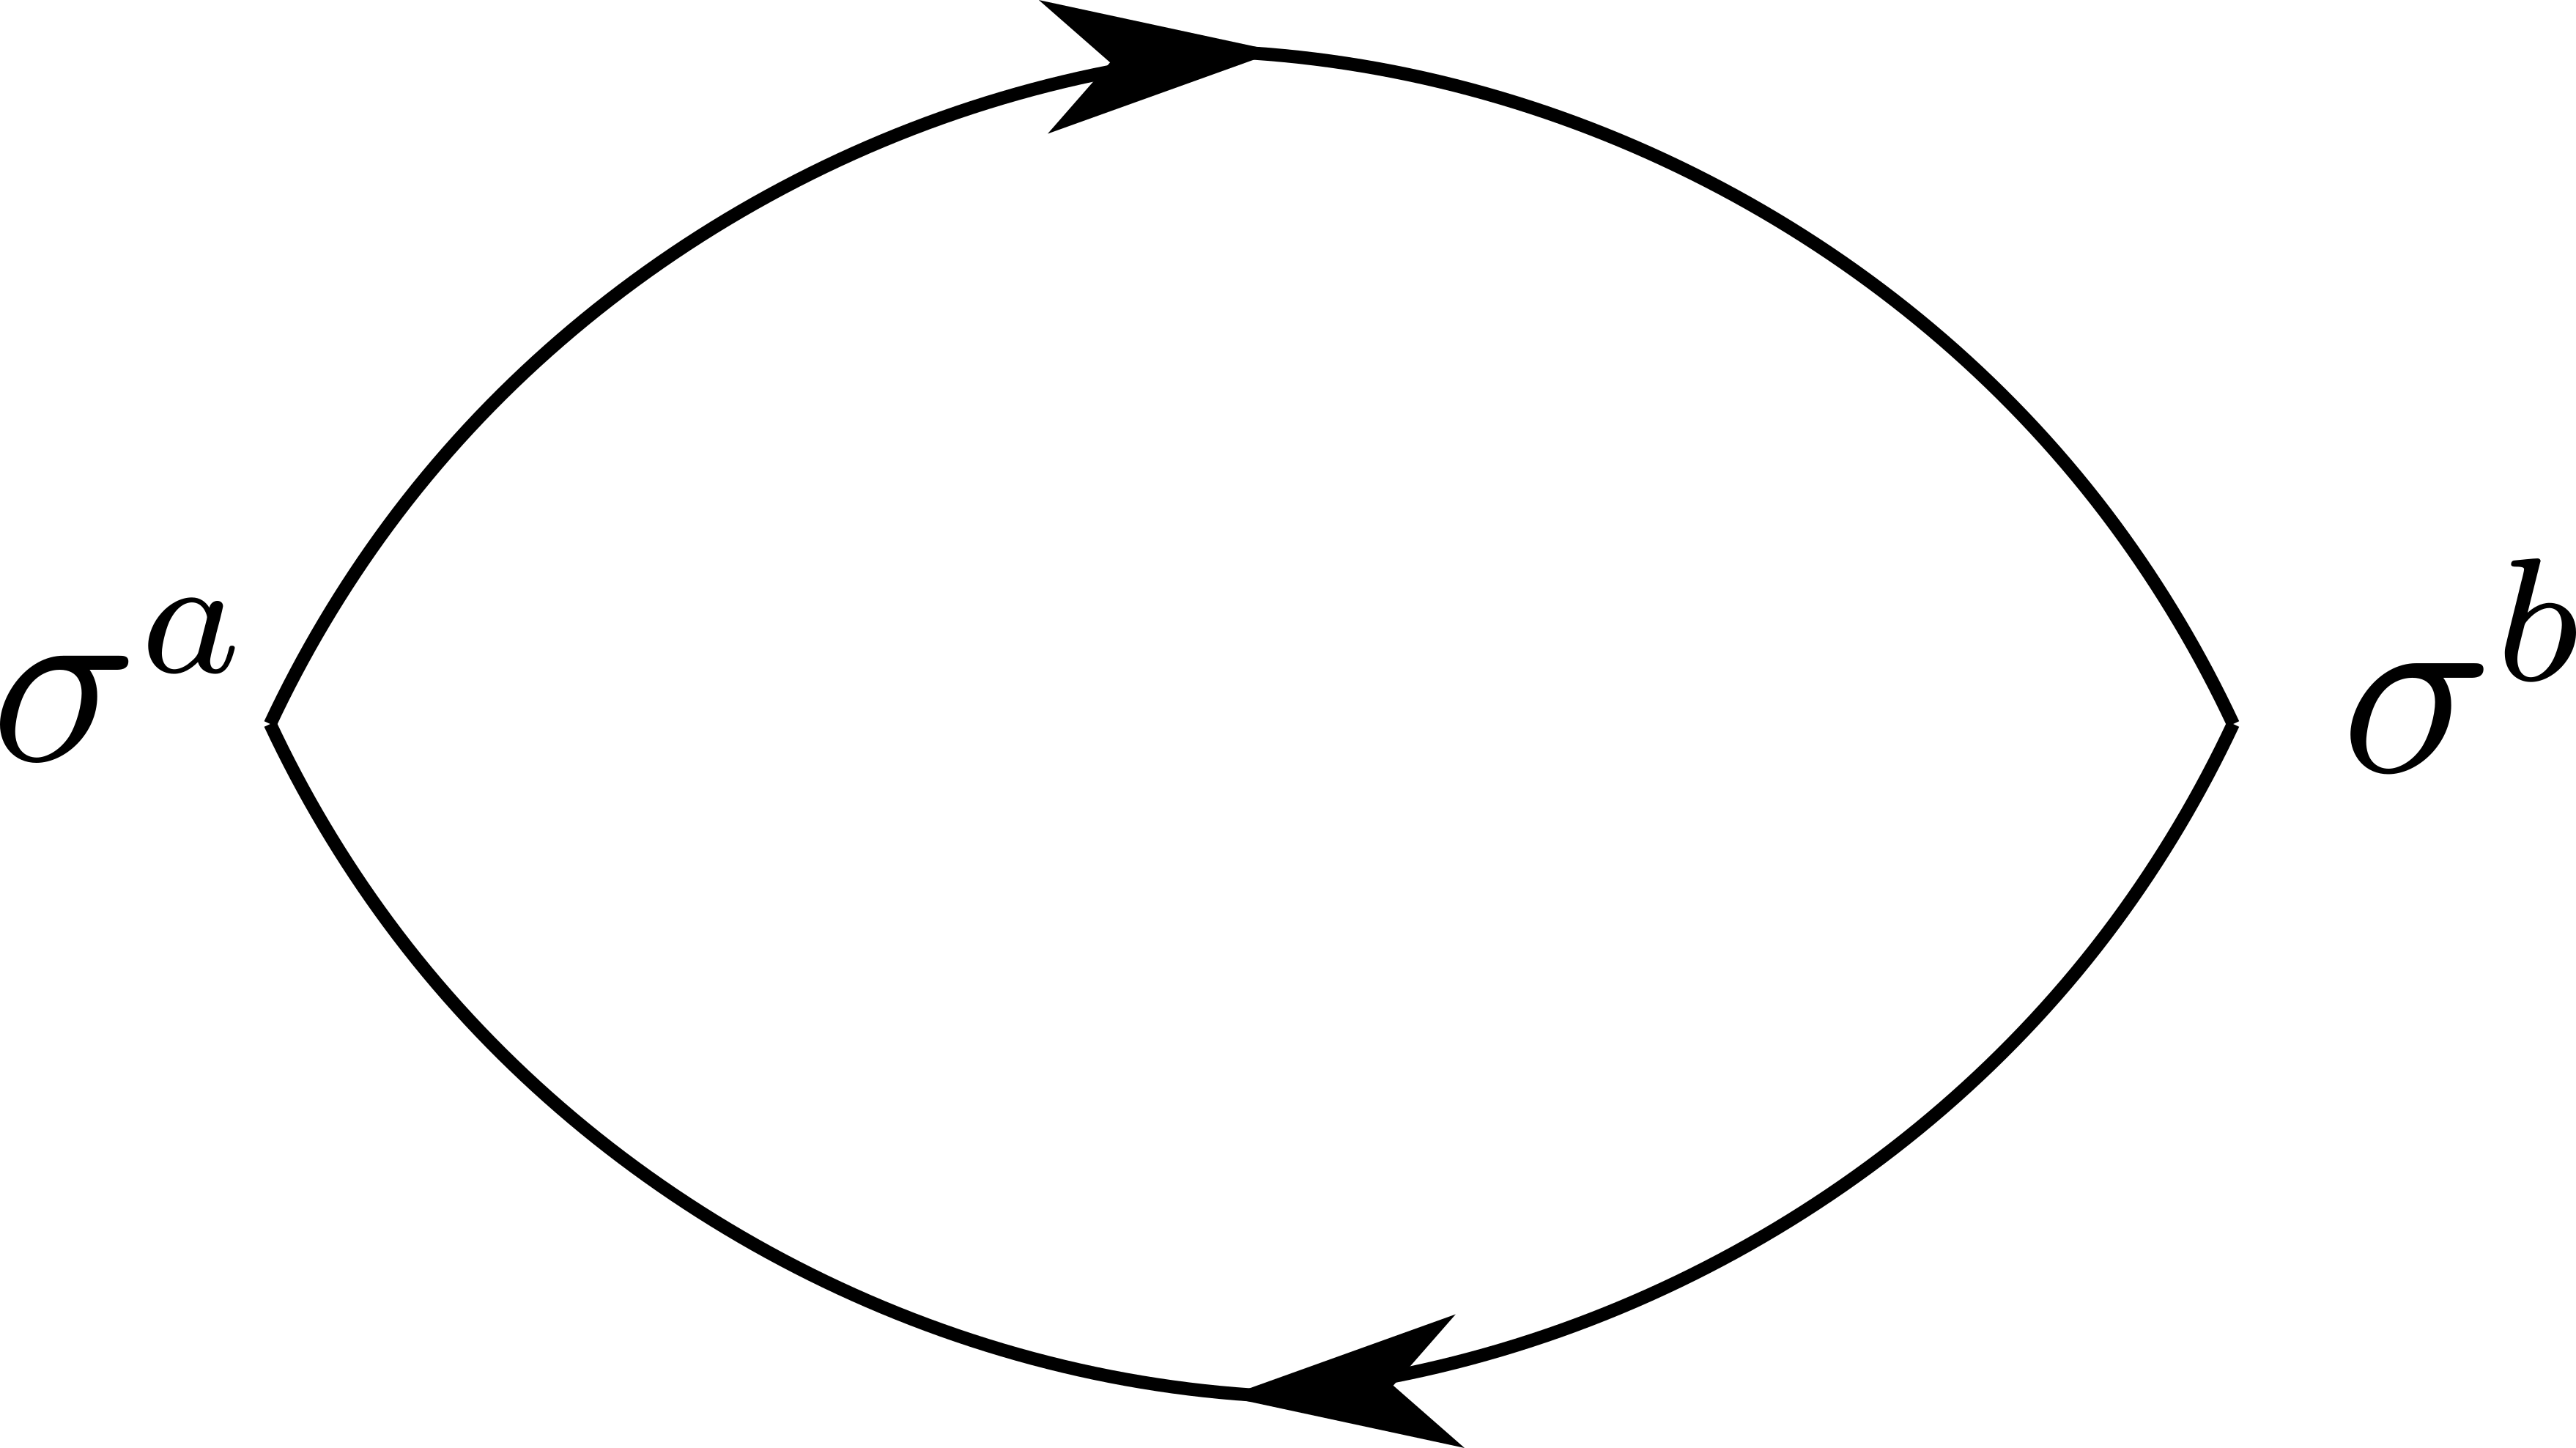
\includegraphics[scale=0.3]{../figures/poppov1.png} 
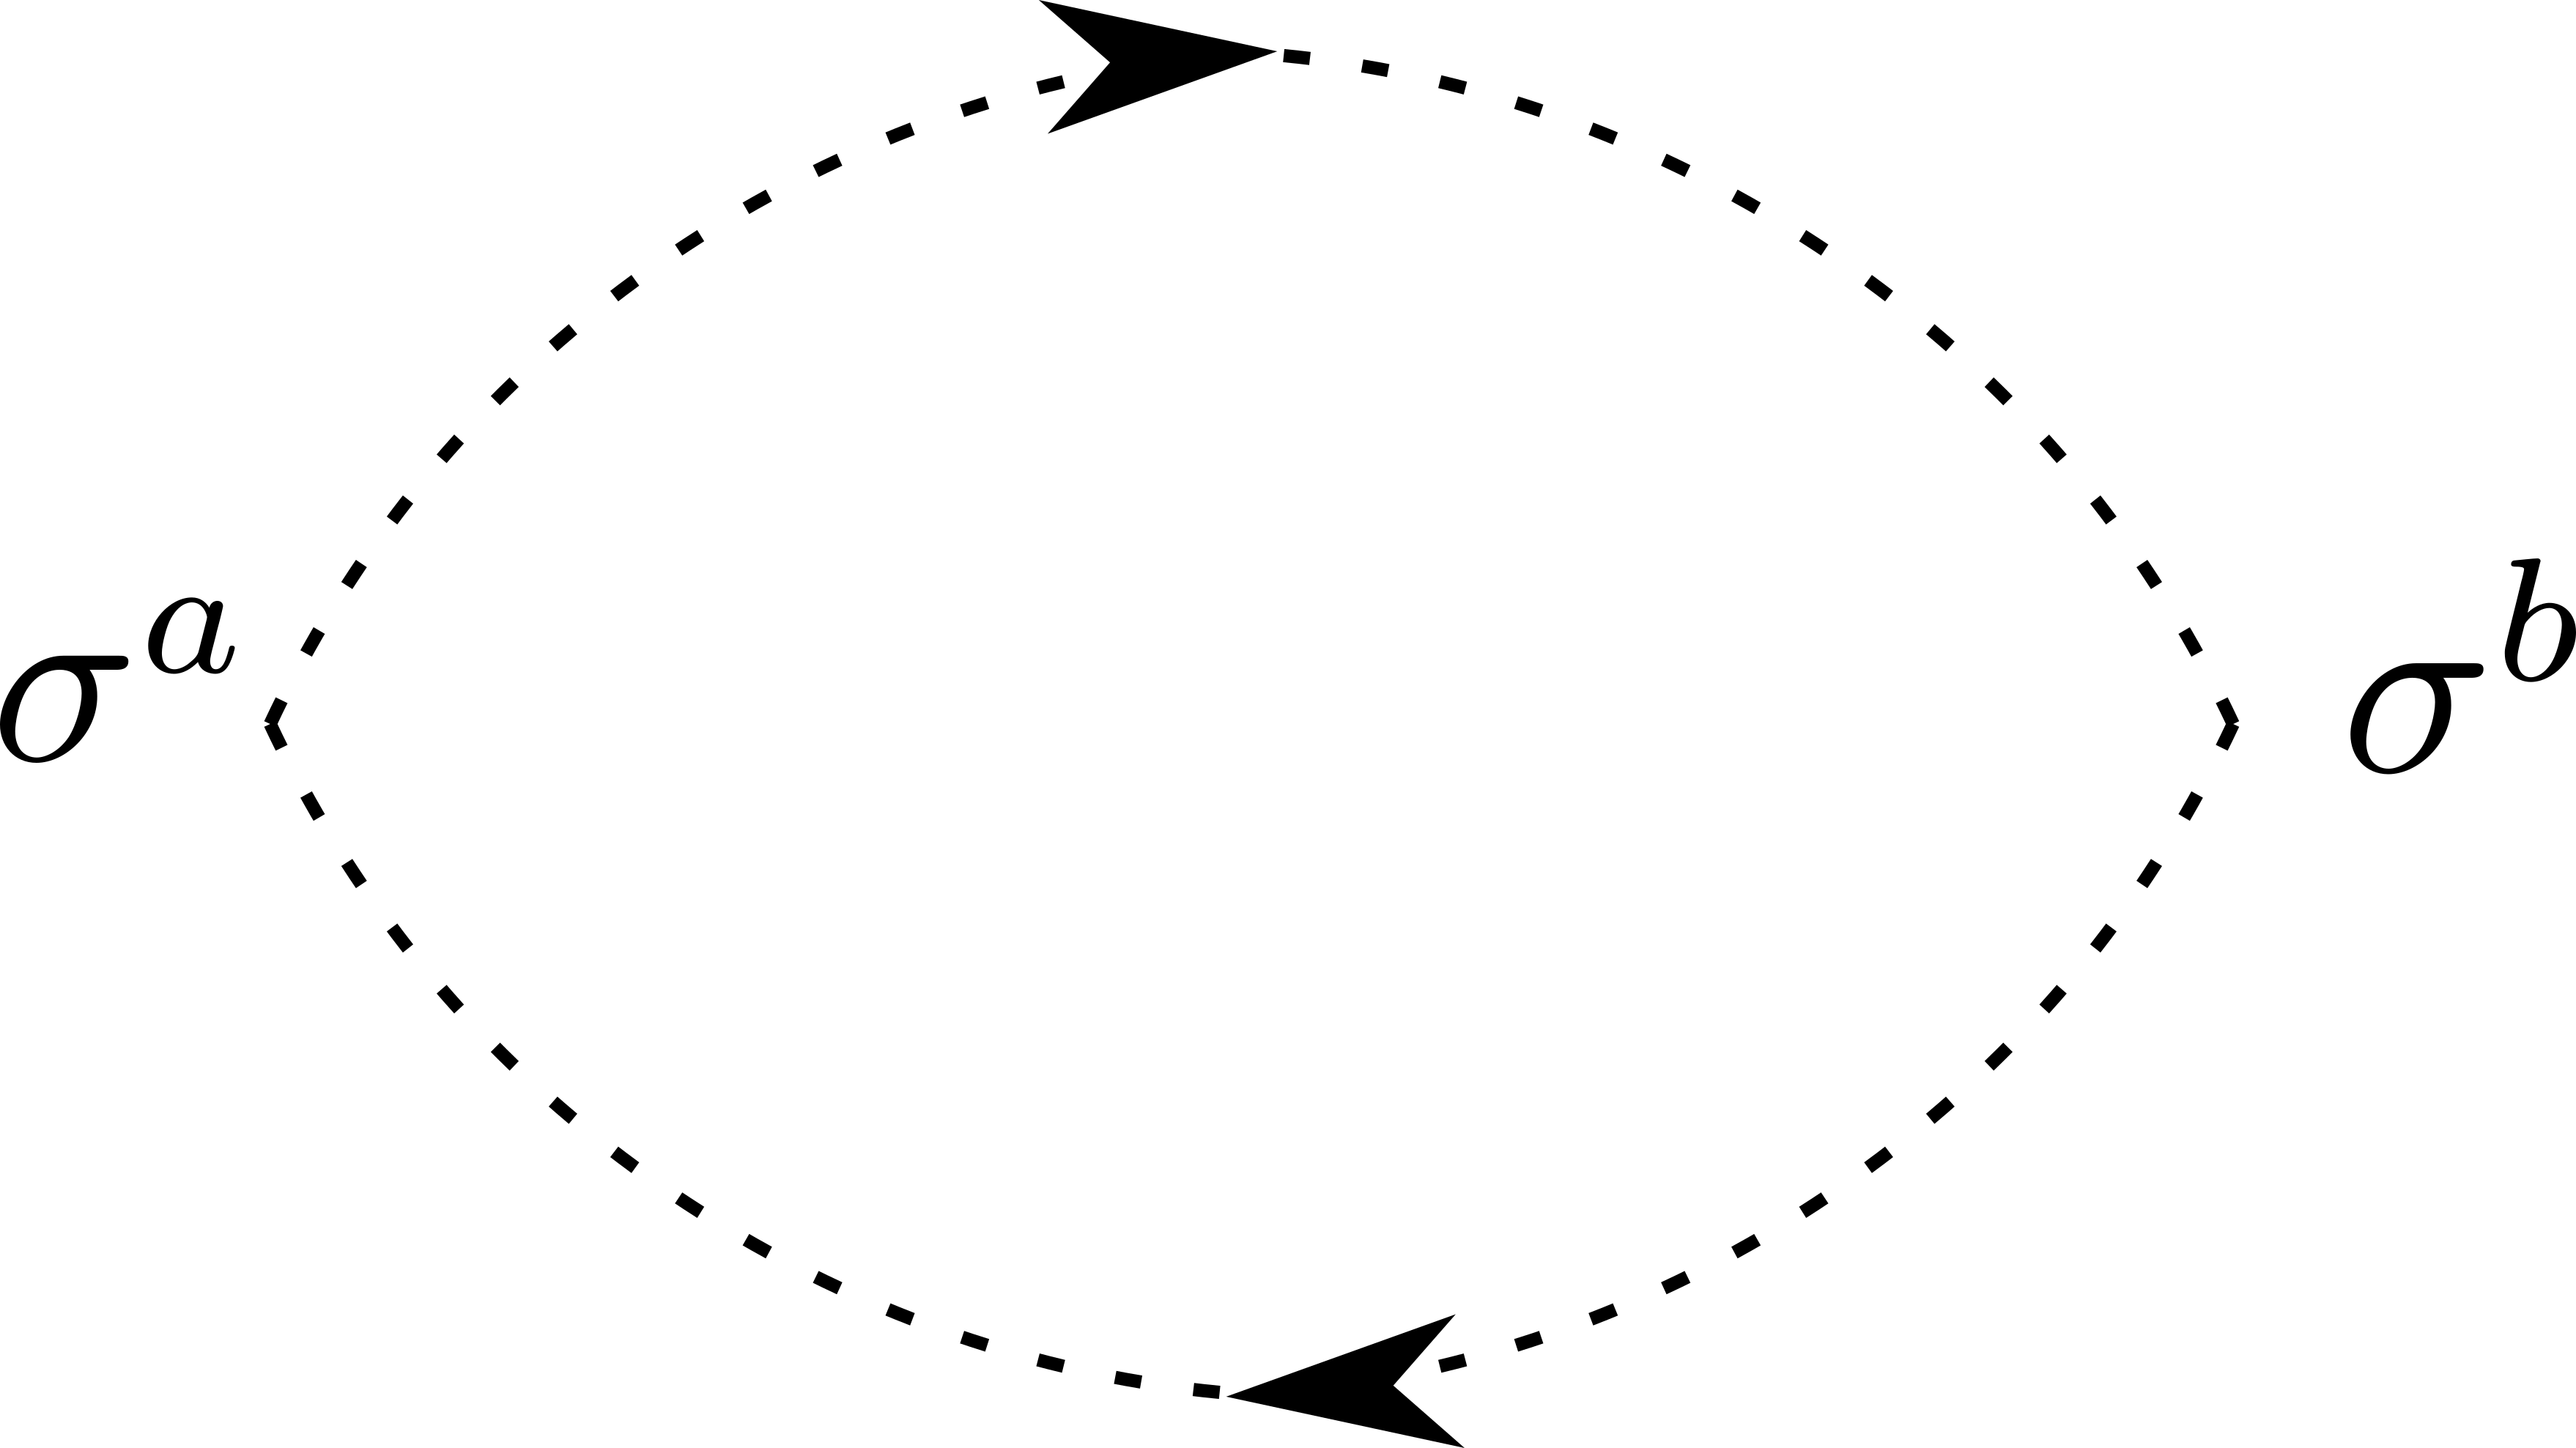
\includegraphics[scale=0.3]{../figures/poppov2.png}
\end{figure}\\\\
The dotted lines are the impurity Greens function, so that diagram gives the impurity contribution to the susceptibility.
Similarly, the solid lines are the conduction electron Greens function.
The first diagram gives
\begin{equation}\begin{aligned}
\chi_c = -k_B T \sum_{k,\omega_n,\phi_0} \bra{\phi_0} \sigma^a G(k,i\omega_n)\sigma^bG_k(i\omega_n)\ket{\phi_0}
\end{aligned}\end{equation}
The sum over the ground states \(\ket{\phi_0}\) constitutes a trace, so we can write it as
\begin{equation}\begin{aligned}
	\chi_c &= -k_B T \sum_{k,\omega_n} \text{Tr}\left[\sigma^a G(k,i\omega_n)\sigma^bG(k,i\omega_n)\right] \\
       &= -2 k_B T \sum_{k,\omega_n} G^2(k,i\omega_n)\\
       &= -2 k_B T \sum_{k,\omega_n} \left(i\omega_n - \epsilon_k\right)^{-2}\\
       &= 2 \sum_k \frac{\:\mathrm{d}}{\:\mathrm{d}\epsilon_k}k_B T\sum_{\omega_n} \left(i\omega_n - \epsilon_k\right)^{-1}
\end{aligned}\end{equation}
Now, it can be shown that
\begin{equation}\begin{aligned}
	k_B T\sum_{\omega_n} \left(i\omega_n - \epsilon_k\right)^{-1} = f(\epsilon_k) - \frac{1}{2}
\end{aligned}\end{equation}
where \(f(\epsilon_k)\) is the FD-distribution at \(\epsilon_k\).
Therefore,
\begin{equation}\begin{aligned}
	\chi_c &=2 \sum_k \frac{\:\mathrm{d}f(\epsilon_k)}{\:\mathrm{d}\epsilon_k}= 2\sum_k \rho(\epsilon_k) = 2 N(0)
\end{aligned}\end{equation}
The second diagram gives
\begin{equation}\begin{aligned}
	\chi_d^{(0)} = -k_B T \sum_{\omega_n} \text{Tr}\left[\sigma^a G_d(i\omega_n)\sigma^bG_d(i\omega_n)\right] \\
\end{aligned}\end{equation}
In the Popov-Fedotov scheme, we replace the impurity Greens function with
\begin{equation}\begin{aligned}
G_d = \frac{1}{i\omega_n - \lambda_d}
\end{aligned}\end{equation}
where \(\lambda_d = i\pi\frac{1}{2\beta}\) is the imaginary chemical potential introduced.
Since this is, for mathematical purposes, the same as the conduction Greens function with \(\lambda_d\) replacing \(\epsilon_k\), we again get
\begin{equation}\begin{aligned}
	\chi^{(0)}_d &=2 \frac{\:\mathrm{d}f(\lambda_d)}{\:\mathrm{d}\lambda_d}= -2\beta\frac{e^{\beta \lambda_d}}{\left(1+e^{\beta \lambda_d}\right)^2} = \beta
\end{aligned}\end{equation}
The first order diagrams are
%\begin{center} 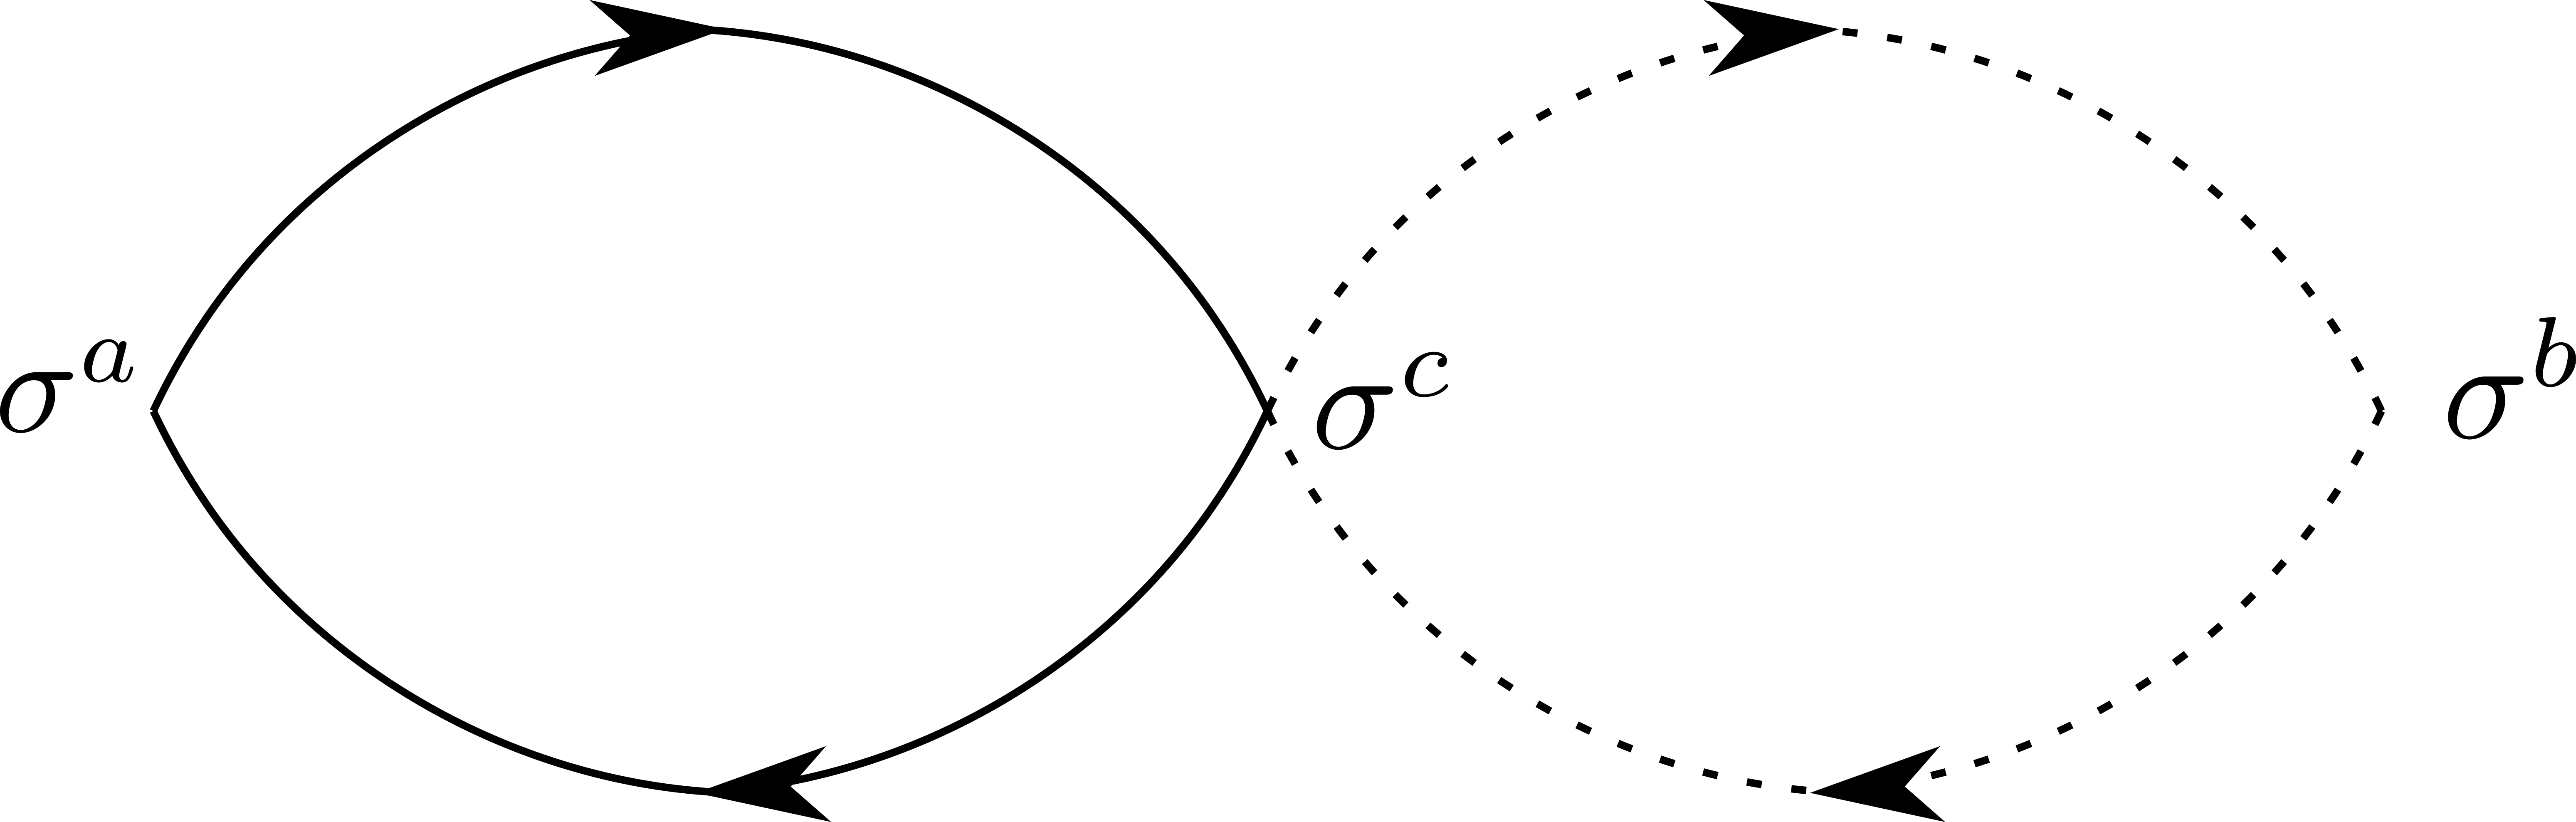
\includegraphics[scale=0.3]{poppov3.png} \end{center}
%\begin{center} 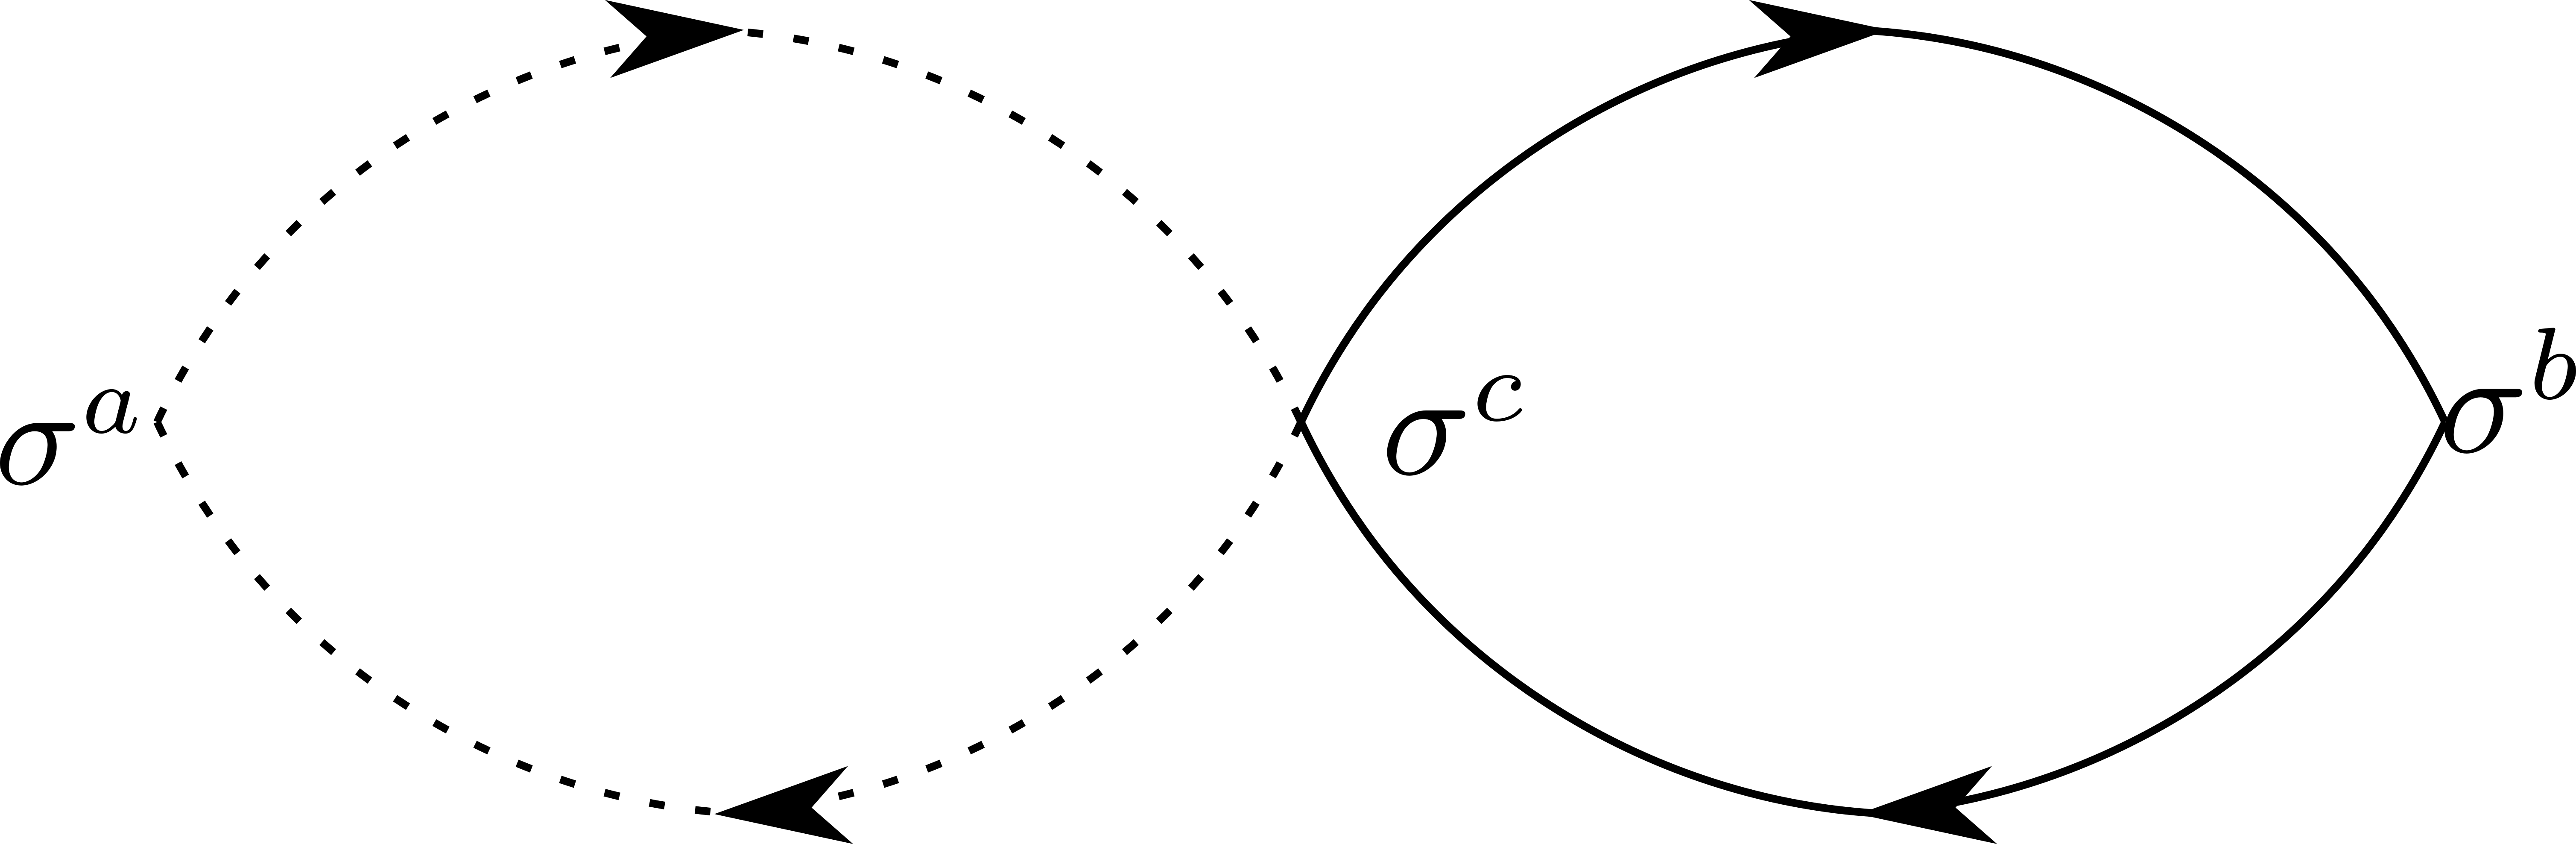
\includegraphics[scale=0.3]{poppov4.png} \end{center}
The first diagram gives
\begin{equation}\begin{aligned}
	\chi^{(1)} = \chi_c \left(-\frac{J}{2}\right) \chi_d = -\beta JN(0)
\end{aligned}\end{equation}
The second one gives
\begin{equation}\begin{aligned}
	\chi_d^{(1)} = \chi_d \left(-\frac{J}{2}\right) \chi_c = -\beta JN(0)
\end{aligned}\end{equation}
The total susceptibility is
\begin{equation}\begin{aligned}
	\chi_d = \chi^{(0)}_d + \chi_d^{(1)} = \beta\left(1 - 2 J N(0)\right)
\end{aligned}\end{equation}
\subsection{Nozières' local Fermi liquid theory}
Wilson's numerical renormalization group calculation showed that the low temperature specific heat contribution from the singlet is linear in temperature
\begin{equation}\begin{aligned}
C_V = \gamma T
\end{aligned}\end{equation}
This suggests that the strong-coupling limit of the Kondo model is a Fermi liquid.\\
The singlet state (\(s=0\)) has an energy
\begin{equation}\begin{aligned}
	E_g = J\left[2\vec S_e \cdot \vec S_d\right] = J\left[S^2 - S_d^2 - S_e^2\right] = J\left[s\left(s+1\right) - \frac{3}{2}\right] = -\frac{3J}{2}
\end{aligned}\end{equation}
Since the interaction term is spherically symmetric, it suffices to consider a one dimensional chain of conduction electrons with the impurity site coupling to the conduction electron at the origin.
This electron forms a singlet with the impurity electron,
\begin{equation}\begin{aligned}
\frac{\ket{0_\uparrow,d\downarrow} - \ket{0_\downarrow,d_\uparrow}}{\sqrt 2}
\end{aligned}\end{equation}
Considering a tight-binding model, the only electron that can hop to the zeroth site is the one on the first site.
The hopping of this electron on to the zeroth site would lead to an energy of
\begin{equation}\begin{aligned}
E_1 = -\frac{3}{2}J + \frac{3}{2}J = 0
\end{aligned}\end{equation}
because the new electron would have the spin opposite to the other electron on the \(0^\text{th}\) site.
This means that breaking the singlet raises the energy by \(\frac{3}{2}J\).
At low temperatures and very large \(J\), this is not possible.
That being said, there can always be virtual fluctuations into excited states.
For example, the impurity electron can tunnel into the conduction band (\(n_d = 0\)) or another conduction electron may scatter into the impurity site (\(n_d = 2\)).
Both these states have zero energy.
With further virtual excitations, it is also possible to go into the triplet state with energy \(\frac{J}{2}\).
What this means is that although the singlet is stable with respect to energy-conserving transitions, the singlet is virtually polarizable, with the help of the site 1 electron.
This induces an interaction on the site 1.
Since the interaction on the site 1 is just a manifestation of the polarizability of the singlet, we can either take the singlet with its polarizability and assume the conduction band to be non-interacting, or we can assume the singlet to be static and take the Fermi sea to have a localised interaction at the site 1.
In the latter picture, we have a frozen singlet (which can be ignored) and an interacting Fermi sea.\\\\
The goal \cite{nozieres} is to calculate the change in phase shift suffered by the conduction electrons in the presence of interactions.
In the absence of interactions, the scattered wavefunction is
\begin{equation}\begin{aligned}
	\label{shift}
	\psi \sim \frac{\sin\left[kr + \delta(E_k)\right]}{r}
\end{aligned}\end{equation}
That is, the phase shift is only a function of the energy.
At the Fermi surface, this value \(\delta(0)\) is \(\frac{\pi}{2}\), as known from the Friedel sum rule.
\begin{equation}\begin{aligned}
n = \sum_\sigma \frac{\delta}{\pi} \implies 1 = \frac{2\delta}{\pi} \implies \delta = \frac{\pi}{2}
\end{aligned}\end{equation}
\(n\) is the number of conduction electrons bound in the resonance and the sum is over the possible quantum numbers (spin in this case).
\(\delta(0)\) can also be obtained directly from eq.~\ref{shift}, by substituting \(k=k_F\) and noting that the isolation of the 0\textsuperscript{th} site means all wavefunctions should shift by \(\Delta r = a\):
\begin{equation}\begin{aligned}
k_F a = \delta(0) \implies \delta(0) = \frac{\pi}{2a} 2 = \frac{\pi}{2}
\end{aligned}\end{equation}
where the formula for \(k_F\) was used.\\\\
In a Fermi gas, the energy levels are separated by
\begin{equation}\begin{aligned}
	\Delta \epsilon = \frac{\partial{\epsilon}}{\partial{k}}\Delta k
\end{aligned}\end{equation}
With the condition that the wavefunction should vanish at the boundary, we have \(\Delta k = k_n - k_{n-1} = \frac{\pi}{L}\).
Hence,
\begin{equation}\begin{aligned}
	\Delta \epsilon = \frac{\partial{\epsilon}}{\partial{k}}\frac{\pi}{L}
\end{aligned}\end{equation}
However, this changes in the presence of the impurity.
Because of eq.~\ref{shift}, the boundary condition becomes
\begin{equation}\begin{aligned}
k_nL + \delta(\epsilon_k) = n\pi \implies k_n = \frac{n\pi}{L} - \frac{\delta}{L} = k_n^0 -\frac{\delta(\epsilon_k)}{L}
\end{aligned}\end{equation}
The energy becomes
\begin{equation}\begin{aligned}
	\epsilon(k) &= \epsilon(k^0) + \frac{\partial{\epsilon}}{\partial{k}}\left(k - k_0\right)\\
		    &= \epsilon_k - \frac{\partial{\epsilon}}{\partial{k}}\frac{\delta(\epsilon_k)}{L}
\end{aligned}\end{equation}
In the Landau formulation of an interacting Fermi liquid, the phase shifts will depend on the quasiparticle occupation probabilities \(n_{k\sigma}\).
Hence,
\begin{equation}\begin{aligned}
	\widetilde \epsilon_\sigma(k) = \epsilon_k - \frac{\partial{\epsilon}}{\partial{k}}\frac{\delta_\sigma(\epsilon_k,\{n_{q,\sigma}\})}{L}
\end{aligned}\end{equation}
In bulk Fermi liquid, we expand the quasiparticle energy in the deviation of the quasiparticle distribution \(n_k\) from the ideal Fermi-Dirac distribution \(n^0_k\),
\begin{equation}\begin{aligned}
	\label{fliq}
	\widetilde \epsilon_p = \underbrace{\epsilon_F}_{\text{Fermi gas}} &+ \overbrace{\frac{p_F^*}{m}\left(p-p_F\right)}^{\text{linear contribution for \textit{p} close to }p_F} \\
								    &+ \underbrace{\sum_{q\sigma}f(p,q)\left(n_q - n^0_q\right)}_{\text{interacting between two quasiparticles at momenta \textit{p} and \textit{q}}}
\end{aligned}\end{equation}
Similarly, for this local Fermi liquid, the phase shift depends on the energy of the quasiparticle \(\widetilde \epsilon\) and the quasiparticle occupation \(n_{q\sigma}\).
Accordingly,
\begin{equation}\begin{aligned}
	\delta_\sigma(\widetilde \epsilon,\{n_{q,\sigma}\}) = \delta_\sigma(\widetilde \epsilon = \epsilon_F, n_k = n^0_k) + \alpha\left(\widetilde \epsilon - \epsilon_F\right) + \Phi \sum_{q\sigma^\prime}\left(n_{q\sigma^\prime} - n^0_{q\sigma^\prime}\right)
\end{aligned}\end{equation}
This is just a Taylor expansion of \(\delta_\sigma\) around \(\tilde \epsilon = \epsilon_F\) and \(n_q = n^0_q\).
\(\Phi\) and \(\alpha\) play the same role as \(f\) and \(\frac{p_F^*}{m}\) in eq.~\ref{fliq}.
Specifically, \(\Phi\) represents the onsite interaction between quasiparticles of  opposite spin and 
\begin{equation}\begin{aligned}
	\alpha = \frac{\:\mathrm{d}\delta_\sigma}{\:\mathrm{d}E}
\end{aligned}\end{equation}
Since \(\Phi\) acts only between quasiparticles of opposite spin, the last term can be simplified by requiring \(\sigma^\prime = -\sigma\),

\begin{equation}\begin{aligned}
	\label{phases}
	\delta_\sigma(\widetilde \epsilon,\{n_{q,\sigma}\}) = \delta_\sigma(\widetilde \epsilon = \epsilon_F, n_k = n^0_k) + \alpha\left(\widetilde \epsilon - \epsilon_F\right) + \Phi \sum_{q}\delta n_{q,-\sigma}
\end{aligned}\end{equation}
Since the singlet is isolated from the Fermi liquid, any change in the chemical potential will not affect the average occupation of the impurity site \(\langle  n_d\rangle\), and since we know that \(\langle  n_d\rangle = \frac{2\delta(0)}{\pi}\), this means that \(\delta(0)\), the phase shift at the Fermi surface, is invariant under a change of the chemical potential.
This in turn means that the resonance scattering (\(\delta = \frac{\pi}{2}\)) will always be pinned to the Fermi surface.
With this knowledge, let us explicitly try to calculate the change in the phase shift at Fermi surface when we change the chemical potential by \(\Delta \mu\).
Before the change in chemical potential,
\begin{equation}\begin{aligned}
\delta^0_\uparrow = \frac{\pi}{2} + \Phi\sum_q \delta n^0_{q\downarrow}
\end{aligned}\end{equation}
Since \(\delta n^0 = n^0 - n^0 =0\),
\begin{equation}\begin{aligned}
\delta^0_\uparrow = \frac{\pi}{2}
\end{aligned}\end{equation}
After the change in chemical potential, \(\epsilon_F^\prime = \epsilon_F + \Delta \mu\) and 
\begin{gather}
N(\mu = 0) = N^0 \\
N(E^\prime = E+\mu) = N(E^\prime = E) + \frac{\:\mathrm{d}N}{\:\mathrm{d}E^\prime}\left(E^\prime - E\right) = N^0 + \rho \Delta \mu\\
\implies \sum_q \delta n_q = N - N^0 = \rho \Delta \mu
\end{gather}
Hence, from eq.~\ref{phases},
\begin{equation}\begin{aligned}
	\delta_\uparrow &= \frac{\pi}{2} + \alpha\left(\epsilon_F^\prime - \epsilon_F\right) + \Phi\sum_q \delta n_{q\downarrow}\\
       &= \delta^0_\uparrow + \alpha\Delta\mu + \Phi \rho \Delta \mu
\end{aligned}\end{equation}
Hence the change in the phase is
\begin{equation}\begin{aligned}
	0 = \Delta \delta_\uparrow = \Delta \mu\left(\alpha + \Phi \rho\right) \implies \alpha = -\Phi\rho
\end{aligned}\end{equation}\\\\
This shows that the interaction term \(\Phi\) is responsible for pinning the resonance at the Fermi level; without that term in the formalism, the occupancy of the impurity site will change.
This is similar to the fact that the interaction term \(f(k,k^\prime)\) in the bulk Fermi liquid is responsible for making the Landau theory invariant under Galilean transformations.\\\\
Now we can calculate the density of states.
From the boundary condition, we have
\begin{equation}\begin{aligned}
n_\sigma = \frac{kL}{\pi} + \frac{\delta_\sigma(E)}{\pi} = n^0 + \frac{\delta_\sigma(E)}{\pi}
\end{aligned}\end{equation}
Hence,
\begin{equation}\begin{aligned}
	\rho &= \frac{\:\mathrm{d}n_\sigma}{\:\mathrm{d}E} = \rho^0 + \frac{1}{\pi}\frac{\:\mathrm{d}\delta_\sigma}{\:\mathrm{d}E} \\
\implies \rho&=\rho^0 + \frac{1}{\pi}\alpha
\end{aligned}\end{equation}
\(\rho^0\) is the density of states in absence of the impurity.
The low temperature specific heat of an ideal Fermi liquid can be shown to be
\begin{equation}\begin{aligned}
C_v^0 = \gamma T = \frac{\pi^2 k_B^2}{3} \mathcal{N}(0) T
\end{aligned}\end{equation}
The interacting Fermi liquid is just a renormalised version of the Fermi gas, with a modified density of states \(\frac{1}{\pi}\alpha\).
Hence, the impurity contribution to the specific heat is
\begin{equation}\begin{aligned}
	C_v &= \frac{\pi^2 k_B^2}{3}\left(\rho_\uparrow + \rho_\downarrow\right) T\\
    &=\frac{2\alpha}{\pi} \frac{\pi^2 k_B^2}{3} T
\end{aligned}\end{equation}
In presence of a magnetic field \(B\), the magnetization is 
\begin{equation}\begin{aligned}
m = \delta n \times \mu
\end{aligned}\end{equation}
where \(\mu\) is the magnetic moment
\begin{equation}\begin{aligned}
\mu = -\frac{g}{2}\mu_B 
\end{aligned}\end{equation}
and \(\delta n\) is the difference in number between up and down electrons
\begin{equation}\begin{aligned}
	\delta n = \langle  n_\uparrow\rangle - \langle  n_\downarrow\rangle = \frac{1}{\pi}\left(\delta_\uparrow - \delta_\downarrow\right)
\end{aligned}\end{equation}
In the presence of the magnetic field, all energies get modified,
\begin{equation}\begin{aligned}
E^B_\sigma = E - \sigma \frac{g\mu_B}{2}B
\end{aligned}\end{equation}
Hence,
\begin{equation}\begin{aligned}
	\sum_k \delta n_{k\sigma} = N_\sigma(E^B_\sigma) - N(E) = \frac{\:\mathrm{d}N}{\:\mathrm{d}E^B}\left(E^B - E\right) = -\rho \frac{g \mu_B}{2}\sigma B
\end{aligned}\end{equation}
This modifies the phase shift at the Fermi surface,
\begin{equation}\begin{aligned}
	\delta_\sigma(\epsilon_F) &= \frac{\pi}{2} + \alpha\left(\epsilon_F - \frac{g \mu_B}{2}\sigma B - \epsilon_F\right) + \Phi\sum_q \delta n_{q,-\sigma}\\
              &= \frac{\pi}{2} - \sigma \frac{g \mu_B}{2}\alpha B + \Phi \rho \frac{g \mu_B}{2}\sigma B\\
              &= \frac{\pi}{2} - 2\alpha\frac{g \mu_B}{2}\sigma B
\end{aligned}\end{equation}
Hence,
\begin{equation}\begin{aligned}
	\delta n = \frac{1}{\pi}\left(\delta_\uparrow - \delta_\downarrow\right) = -\frac{4\alpha B}{\pi}\frac{g \mu_B}{2}
\end{aligned}\end{equation}
The susceptibility is
\begin{equation}\begin{aligned}
	\chi = \frac{\partial{m}}{\partial{B}} = \frac{\partial{}}{\partial{B}}\mu\delta n = \frac{4\alpha}{\pi}\left(\frac{g \mu_B}{2}\right)^2
\end{aligned}\end{equation}

The susceptibility for an ideal Fermi gas can be calculated similarly.
The additional energy of an electron with spin \(\sigma\) in a magnetic field \(B\) is \(-\sigma \frac{g}{2}\mu_B B\).
The magnetization induced at the Fermi surface is \(\delta n \times \mu\), where \(\mu\) is the magnetic moment
\begin{equation}\begin{aligned}
\mu = -\frac{g}{2}\mu_B 
\end{aligned}\end{equation}
and \(\delta n\) is the difference in number between up and down electrons
\begin{equation}\begin{aligned}
\delta n = n_\uparrow(0) - n_\downarrow(0) = n_\uparrow(\epsilon_F - \frac{g}{2}\mu_B B) - n_\downarrow(\epsilon_F + \frac{g}{2}\mu_B B) = -\frac{1}{2}\mathcal{N}(0)gB \mu_B
\end{aligned}\end{equation}
\(\mathcal{N}(0) = \frac{\partial{n}}{\partial{E}}\bigg |_{\epsilon_F}\) is the density of states at the Fermi energy and the \(\frac{1}{2}\) is because we are counting electrons of a particular spin only.
Therefore,
\begin{equation}\begin{aligned}
	m = \delta n \times \mu = \mathcal{N}(0)\left(\frac{g}{2} \mu_B\right)^2B
\end{aligned}\end{equation}
The magnetic susceptibility comes out to be 
\begin{equation}\begin{aligned}
	\chi^0 = \frac{\partial{m}}{\partial{B}}\bigg |_{B \rightarrow 0} = \mathcal{N}(0)\left(\frac{g}{2} \mu_B\right)^2
\end{aligned}\end{equation}
The Wilson ratio \(R\) can now be computed,
\begin{equation}\begin{aligned}
R = \frac{\chi/\chi_0}{C_v/C_v^0} = \frac{4\alpha/\pi\mathcal{N}(0)}{2\alpha/\pi\mathcal{N}(0)} = 2
\end{aligned}\end{equation}

\section{Numerical renormalization group calculation}
Wilson's idea \cite{wilson} was to remove the limitations of the perturbative nature of Anderson's scaling method.
To that end, we transformed the Hamiltonian into a one-dimensional chain, and then iteratively diagonalised chains of increasing length.
The Hamiltonian we are working with is
\begin{equation}\begin{aligned}
H = \sum_k \epsilon_k n_k + J \vec S_d \cdot \vec \sigma_e
\end{aligned}\end{equation}
where \(\vec \sigma_e = \sum_{k_1,k_2,\alpha\beta}c^\dagger_{k_1\alpha}\vec \sigma_{\alpha\beta}c_{k_2,\beta}\) is the conduction electron spin at the origin.
This assumes that the exchange interaction \(J(k,k^\prime\) is independent of spin.
To form the linear chain, we construct a new basis in which to express the conduction electron part \(H_c\), out of the states \(\ket{0},H_c\ket{0},H_c^2\ket{0},...\).
\(\ket{0}\) is the origin site, where the impurity resides.
The first member of the new basis is \(\ket{0}\).
The next member is taken to be some state in the subspace of \(\ket{0}\) and \(H_c\ket{0}\),
\begin{equation}\begin{aligned}
	\ket{1} = \left(\lambda_1 H_c\ket{0} + \lambda_2\ket{0}\right)
\end{aligned}\end{equation}
This is a general form for any ket in the subspace spanned by \(\ket{0}\) and \(H_c\ket{0}\).
Since we want the state to be normalised , we can shift one of the parameters to the denominator:
\begin{equation}\begin{aligned}
	\ket{1} = \frac{1}{\gamma_0}\left(H_c\ket{0} + \lambda\ket{0}\right)
\end{aligned}\end{equation}
where \(\gamma_0\) sets \(\langle 1|1\rangle = 1\).
The remaining parameter is set by requiring \(\langle 1|0\rangle = 0\).
That gives
\begin{equation}\begin{aligned}
	\lambda = -\langle 0|H_c|0\rangle
\end{aligned}\end{equation}
Therefore,
\begin{equation}\begin{aligned}
	\ket{1} = \frac{1}{\gamma_0}\left(H_c\ket{0} -\langle 0|H_c|0\rangle\ket{0}\right)
\end{aligned}\end{equation}
The general state can be shown to be
\begin{equation}\begin{aligned}
	\label{chain}
	\ket{n+1} = \frac{1}{\gamma_n}\left(H_c \ket{n} - \ket{n}\langle  n|H_c|n-1\rangle-\ket{n-1}\langle  n-1|H_c|n\rangle\right)
\end{aligned}\end{equation}
From eq.~\ref{chain}, by multiplying \(\bra{n^\prime}\) from left, we get
\begin{equation}\begin{aligned}
	\delta_{n^\prime,n+1} = \frac{1}{\gamma_n}\left[\left(H_c\right)_{n^\prime,n} + \left(H_c\right)_{n,n-1}\delta_{n^\prime,n} + \left(H_c\right)_{n-1,n}\delta_{n^\prime,n-1}\right]
\end{aligned}\end{equation}
Clearly, for \(n^\prime < n-1\) or \(n^\prime > n+1\), we get
\begin{equation}\begin{aligned}
	\left(H_c\right)_{n^\prime,n} = 0
\end{aligned}\end{equation}
so the only non-zero terms are for \(n^\prime = n-1,n,n+1\).
For \(n^\prime = n+1\) gives
\begin{equation}\begin{aligned}
	\left(H_c\right)_{n+1,n} = \gamma_n
\end{aligned}\end{equation}
Taking the complex conjugate of this gives
\begin{equation}\begin{aligned}
	\gamma_n^* = \left(H_c^\dagger\right)_{n,n+1} = \left(H_c\right)_{n,n+1}
\end{aligned}\end{equation}
Defining 
\begin{equation}\begin{aligned}
	\left(H_c\right)_{n,n} = \epsilon_n
\end{aligned}\end{equation}
we can write
\begin{equation}\begin{aligned}
H_c &= \sum_{n_1,n_2} \ket{n_1}\bra{n_1} H_c \ket{n_2}\bra{n_2}\\
    &= \sum_{n}\epsilon_n \ket{n}\bra{n} + \sum_{n}\left(\gamma_n\ket{n} \bra{n+1}+ \gamma^*_n\ket{n+1} \bra{n}\right)\\
    &= \sum_{n}\epsilon_n \hat n_n + \sum_{n}\left(\gamma_nc^\dagger_n c_{n+1}+ \gamma^*_nc^\dagger_{n+1} c_{n}\right)
\end{aligned}\end{equation}
The diagonalization of these chains become impossible for \(n>8\).
To remedy this problem, Wilson, after diagonalization a chain of a particular length, retained only the lowest parts of the spectrum, and the Hamiltonian for the next stage was formed out of these low-lying states.
This keeps the size of the Hilber space (and hence the matrices) manageable.
Another problem is that as one goes on adding sites to the chain, the couplings need to die off, otherwise this process will never converge.

\subsubsection{Logarithmic discretization}
First, note that up to first order
\begin{equation}\begin{aligned}
	\epsilon_k = \epsilon_F + (k-k_F)\frac{\partial{\epsilon_k}}{\partial{k}}
\end{aligned}\end{equation}
By choosing \(k_F = \epsilon_F = 0\), we get \(\epsilon_k = k\).\\\\
Wilson divided the conduction band into patches, \([\Lambda^{-(n+1)},\Lambda^{-n}]\), for \(n=1,2,3..\).
The width of each interval is
\begin{equation}\begin{aligned}
	d_n = \Lambda^{-n}\left(1-\Lambda^{-1}\right)
\end{aligned}\end{equation}
We can now define orthogonal functions in this \(n^\text{th}\) interval \(k \in [\Lambda^{-(n+1)},\Lambda^{-n}]\),
\begin{equation}\begin{aligned}
\psi_{m,n}(k) = \frac{1}{\sqrt{d_n}} \exp\left\{\frac{2\pi i m}{d_n} k\right\}
\end{aligned}\end{equation}
They allows us to define a new set of creation operators,
\begin{equation}\begin{aligned}
a^\dagger_{m,n} = \sum_k \psi_m(k)c^\dagger_k
\end{aligned}\end{equation}
Similarly functions can be defined in the negative interval \(-k \in[\Lambda^{-(n+1)},\Lambda^{-n}]\).
\begin{gather}
    \phi_{m,n}(k) = \frac{1}{\sqrt{d_n}} \exp\left\{-\frac{2\pi i m}{d_n} k\right\}\\
    b^\dagger_{m,n} = \sum_k \phi_m(k)c^\dagger_k
\end{gather}
Then,
\begin{equation}\begin{aligned}
	a^\dagger_{m,n} + b^\dagger_{m,n} = \frac{2}{\sqrt{d_n}}\sum_{\pm k \in []} \cos \left(\frac{2\pi mk}{d_n}\right) c^\dagger_k
\end{aligned}\end{equation}
Summing over \(n\) involves summing over all momenta.
\begin{equation}\begin{aligned}
	\label{zerom}
	\sum_n \left(a^\dagger_{m,n} + b^\dagger_{m,n}\right) &= \frac{2}{\sqrt{d_n}}\sum_{k} \cos \left(\frac{2\pi mk}{d_n}\right) c^\dagger_k\\
	\implies \sum_n \left(a^\dagger_{0,n} + b^\dagger_{0,n}\right) &= \frac{2}{\sqrt{d_n}}\sum_{k} c^\dagger_k\\
\end{aligned}\end{equation}
For the momentum-independent \(J(k,k^\prime)\), the coupling term involves.
\begin{equation}\begin{aligned}
\sum_{k,q}c^\dagger_k c_q = \sum_{k}c^\dagger_k \sum_{q}c_q
\end{aligned}\end{equation}
Looking at eq.~\ref{zerom}, we see that the impurity spin is coupled only to the \(m=0\) operators.
This is where the approximation comes in, in Wilson's scheme.
All the \(m\) values other than \(m=0\) are ignored.\\\\
Wilson chose
\begin{equation}\begin{aligned}
\epsilon_n = 0, \gamma = D^\prime \Lambda^\frac{-n}{2}
\end{aligned}\end{equation}
with \(\Lambda>1\).
The Hamiltonian for \(N\) sites then turns out to be
\begin{equation}\begin{aligned}
	\label{run}
	H_N = D^\prime \sum_{n=0}^{N-1} \Lambda^{-\frac{n}{2}}\left(c^\dagger_n c_{n+1}+c^\dagger_{n+1} c_{n}\right) + 2 J \vec S_d \cdot \vec S_e
\end{aligned}\end{equation}
The next step involves adding another site to the chain.
The next Hamiltonian is hence
\begin{equation}\begin{aligned}
	H_{N+1} = H_N + D^\prime \Lambda^{-\frac{N}{2}}\left(c^\dagger_N c_{N+1}+c^\dagger_{N+1} c_{N}\right)
\end{aligned}\end{equation}
To compare the couplings, and hence the Hamiltonians, at each value of \(N\), we need to rescale the Hamiltonians \(H_N\) so that the lowest energy scale is independent of the running index \(N\).
Looking at eq.~\ref{run}, the lowest energy scale is \(\Gamma_N = D^\prime \Lambda^{-\frac{N-1}{2}}\).
Hence, the rescaled Hamiltonian is
\begin{equation}\begin{aligned}
\overline H_N = \frac{H_N}{\Gamma_N} = \frac{\Lambda^{\frac{N-1}{2}}}{D^\prime} H_N
\end{aligned}\end{equation}
The utility can be seen by noting the relation between \(\overline H_{N+1}\) and \(\overline H_N\),
\begin{equation}\begin{aligned}
	\label{rec}
	\overline H_{N+1} &= \frac{\Lambda^{\frac{N}{2}}}{D^\prime}\left[H_N + \Lambda^{\frac{-N}{2}}D^\prime\left(c^\dagger_N c_{N+1}+c^\dagger_{N+1} c_{N}\right)\right]\\
	\implies \overline H_{N+1} &= \Lambda^\frac{1}{2}\overline H_N + \left(c^\dagger_N c_{N+1}+c^\dagger_{N+1} c_{N}\right)
\end{aligned}\end{equation}
In the series of Hamiltonians \(\{H_N\}\), the couplings to the extra site are all same, so the lowest energy scales are all of the same order.
This allows us to construct a flow of the Hamiltonians.
The real Hamiltonian is the unscaled one, so it is given by
\begin{equation}\begin{aligned}
H = \lim_{N \rightarrow \infty} H_N = \lim_{N \rightarrow \infty} D^\prime \Lambda^\frac{1-N}{2} \overline H_N
\end{aligned}\end{equation}
Since \(\overline H_N\) is exactly diagonalised with a spectrum \(\{E_m,\ket{m}\}\), it can be written down as
\begin{equation}\begin{aligned}
\overline H_N = \sum_m E_m \ket{m}\bra{m}
\end{aligned}\end{equation}
The next Hamiltonian is then
\begin{equation}\begin{aligned}
	\overline H_{N+1} = \Lambda^\frac{1}{2} \sum_m E_m \ket{m}\bra{m} + \sum_{m.m^\prime}\left( C(m,m^\prime) \ket{m}\bra{m^\prime} + \text{h.c.}\right)
\end{aligned}\end{equation}
This is the same equation as eq.~\ref{rec}, with \(\overline H_N\) expressed in its eigenbasis and the creation and annihilation operators also expressed in that basis; the \(C(m,m^\prime)\) are just the matrix elements of \(c\) and \(c^\dagger\) in that basis.\\\\
To check whether the guesses about the fixed points are true, Wilson did the following.
He set \(J=0.009\) and then then calculated the lowest excitations of the Hamiltonians obtained from the NRG in the limit of large \(N\).
They indeed correspond to the excitations of the Kondo hamiltonian at \(J = \infty\), meaning that under the application of the NRG, the \(J=0.009\) Hamiltonian flowed to the fixed-point Hamiltonian \(J = \infty\).
\section{Correspondence between the Kondo model fixed-point and a local Fermi liquid}
\subsubsection{Local Fermi liquid}
The fixed-point Hamiltonians \cite{hewsonp} are found to represent interacting Fermi liquids.
The effective Hamiltonian can be shown to resemble the Anderson model, but with modified parameters,
\begin{equation}\begin{aligned}
H_\text{eff} = \sum_k \epsilon_k n_k + \sum_k{V_k c^\dagger_d c_k + \text{h.c.}} + U n_{d\uparrow}n_{d\downarrow}
\end{aligned}\end{equation}
The parameters \(\epsilon_k,V_k,U\) are not the same as the Anderson model we start with, but I am using the same symbols for convenience.
The interaction term \(U\) is the leading irrelevant operator near the low-energy fixed point.
For \(T \rightarrow 0\), assuming only single excitations, the interacting term will not get invoked.\\\\
Under mean-field,
\begin{equation}\begin{aligned}
n_{d\uparrow}n_{d\downarrow} &\approx \langle  n_{d\uparrow}\rangle n_{d\downarrow} + \langle  n_{d\uparrow}\rangle n_{d\downarrow} - \langle  n_{d\uparrow}\rangle\langle  n_{d\downarrow}\rangle\\
\implies \langle  n_{d\uparrow}n_{d\downarrow}\rangle &= \langle  n_{d\uparrow}\rangle\langle  n_{d\downarrow}\rangle\\
						    &= \sum_{k,q}\langle  n_{k\sigma}\rangle \langle  n_{q,-\sigma}\rangle\\
\end{aligned}\end{equation}
where \(N\) is the number of sites.
Note that the number of excitations, \(\langle  n_q\rangle\) has to be defined differently for the states above and below the Fermi surface.
For excited states above \(\epsilon_F\), the number of excitations is given usually:
\begin{equation}\begin{aligned}
	\langle  n_q^>\rangle = \bra{\psi^>}c^\dagger_k c_k\ket{\psi^>} = n^p_k
\end{aligned}\end{equation}
where \(n^p_k\) stands for the number of particles.
For states below \(\epsilon_F\), however, we need to count the number of holes:
\begin{equation}\begin{aligned}
	\langle  n_q^<\rangle = \bra{\psi^<}c^\dagger_k c_k\ket{\psi^<} = -\bra{\psi^<}c_k c^\dagger_k \ket{\psi^<} = -n^h_k
\end{aligned}\end{equation}
where \(n^h_k\) stands for the number of holes.
We can thus define a generalized excitation:
\begin{equation}\begin{aligned}
	\langle \delta n_{k,\sigma}\rangle = \begin{cases} n^p_k, &\epsilon_k > \epsilon_F\\ -n^h_k, &\epsilon_k < \epsilon_F\end{cases}
\end{aligned}\end{equation}
Replacing the quasiparticle excitations with their expectation values, the effective one-particle energy becomes
\begin{equation}\begin{aligned}
	\epsilon_{k\sigma} = \epsilon_k + U\sum_q \langle \delta n_{q,-\sigma}\rangle \equiv \epsilon_k + U\langle \delta n_{-\sigma}\rangle
\end{aligned}\end{equation}
This is analogous to the Landau quasiparticle energy functional, eq.~\ref{temp_en}, \(U\) acting as the interaction between the quasiparticles.
\(\delta n > 0\) acts as the excitations from the ground state.
\\\\
The interacting density of states is
\begin{equation}\begin{aligned}
	\label{dosint}
	\rho_{d\sigma}(\omega) = \frac{\Delta}{\pi}\frac{1}{\left(\omega - \epsilon_d^*\right)^2 + \Delta^2}
\end{aligned}\end{equation}
where \(\epsilon_d^* = \epsilon_d + U\langle \delta n_{-\sigma}\rangle\).

\subsubsection{Calculation of \(C_v\)}
To calculate the specific heat, \(C_v = \frac{\:\mathrm{d}\langle E\rangle}{\:\mathrm{d}T}\), note that a change in temperature would modify the quasiparticle distribution \(\delta n_{k\sigma}\) and hence the quasiparticle energies \(\epsilon_{k\sigma}\).
This leads to a complicated feedback effect.
However, at low temperatures, higher order excitations will be very low and we can approximate by considering only the variation in the distribution:
\begin{equation}\begin{aligned}
	\frac{\:\mathrm{d}\langle E\rangle}{\:\mathrm{d}T} &= \sum_{k,\sigma}\epsilon_{k\sigma}\frac{\:\mathrm{d}\langle \delta n_{k\sigma}\rangle}{\:\mathrm{d}T}\\
\end{aligned}\end{equation}
Since the quasiparticle excitations are adiabatically connected to the free electron excitations, \(\langle \delta n_{k\sigma}\rangle\) will follow a Fermi-Dirac distribution:
\begin{equation}\begin{aligned}
	\langle \delta n_{k\sigma}\rangle(T) &= \frac{1}{e^{\beta\epsilon_{k\sigma}} + 1}\\
	\implies \frac{\:\mathrm{d}\langle \delta n_{k\sigma}\rangle}{\:\mathrm{d}T} &= \frac{e^{\beta\epsilon_{k\sigma}}}{\left(e^{\beta\epsilon_{k\sigma}} + 1\right)^2}\left[\frac{1}{k_B T^2}\epsilon_{k\sigma} -\frac{1}{k_B T}\left(2\epsilon_{k\sigma} - \epsilon_k\right)\frac{\:\mathrm{d}\langle \delta n_{k\sigma}\rangle}{\:\mathrm{d}T}\right]
\end{aligned}\end{equation}
At sufficiently low temperatures, the first term will dominate over the others (\(T^{-2} \gg T^{-1}\)).
Hence the low temperature specific heat can be written as
\begin{equation}\begin{aligned}
	\frac{\:\mathrm{d}\langle E\rangle}{\:\mathrm{d}T} &= \sum_{k,\sigma}\epsilon_{k\sigma}\frac{e^{\beta\epsilon_{k\sigma}}}{\left(e^{\beta\epsilon_{k\sigma}} + 1\right)^2}\frac{1}{k_B T^2}\epsilon_{k\sigma}\\
			&= \frac{1}{k_B T^2}\sum_{k,\sigma}\epsilon_{k\sigma}^2\frac{e^{\beta\epsilon_{k\sigma}}}{\left(e^{\beta\epsilon_{k\sigma}} + 1\right)^2}\\
			&=\frac{1}{k_B T^2}\sum_{\sigma}\int d\epsilon_\sigma \rho(\epsilon_\sigma) \epsilon_{\sigma}^2\frac{e^{\beta\epsilon_{k\sigma}}}{\left(e^{\beta\epsilon_{k\sigma}} + 1\right)^2}
\end{aligned}\end{equation}
The function \(\frac{e^{\beta\epsilon_{k\sigma}}}{\left(e^{\beta\epsilon_{k\sigma}} + 1\right)^2}\) is very sharply peaked at the Fermi surface \(\epsilon_\sigma = 0\).
Therefore we can replace the density of states by its value at the Fermi surface.
\begin{equation}\begin{aligned}
	\frac{\:\mathrm{d}\langle E\rangle}{\:\mathrm{d}T} &=\frac{1}{k_B T^2}\sum_{\sigma}\rho_\sigma(0) \int_{-\infty}^\infty d\epsilon_\sigma\epsilon_{\sigma}^2\frac{e^{\beta\epsilon_{k\sigma}}}{\left(e^{\beta\epsilon_{k\sigma}} + 1\right)^2}\\
        &=-\frac{1}{T}\sum_{\sigma}\rho_\sigma(0) \int_{-\infty}^\infty  d\epsilon_\sigma \epsilon_{\sigma}^2f^\prime(\epsilon_\sigma)\\
        &=-\frac{1}{T}\sum_{\sigma}\rho_\sigma(0) \int_1^0 df \epsilon_{\sigma}^2
\end{aligned}\end{equation}
\(f(\epsilon_\sigma)\) is the Fermi-Dirac distribution.
Note that
\begin{equation}\begin{aligned}
	\epsilon = k_B T\ln \left(f^{-1} - 1\right)\implies \epsilon^2 =k_B^2 T^2\left[\ln \left(f^{-1} - 1\right)\right]^2
\end{aligned}\end{equation}
Therefore,
\begin{equation}\begin{aligned}
	\frac{\:\mathrm{d}\langle E\rangle}{\:\mathrm{d}T} &=-k_B^2 T\sum_{\sigma}\rho_\sigma(0) \int_1^0 df \left[\ln \left(f^{-1} - 1\right)\right]^2
\end{aligned}\end{equation}
The remaining integral gives \(-\frac{\pi^2}{3}\).
For \(T \rightarrow 0\), quasiparticle excitations will be absent and we can write \(\rho_\uparrow = \rho_\downarrow = \rho_d\):
\begin{equation}\begin{aligned}
	\frac{\:\mathrm{d}\langle E\rangle}{\:\mathrm{d}T} &=k_B^2 T\sum_{\sigma}\rho_d(0) \frac{\pi^2}{3}\\
        &=2k_B^2 T\rho_d(0) \frac{\pi^2}{3}\\
        &= \gamma_\text{imp}T
\end{aligned}\end{equation}
where
\begin{equation}\begin{aligned}
\gamma_\text{imp} \equiv \frac{C_v}{T} = \frac{2\pi^2}{3}k_B^2\rho_d(0) 
\end{aligned}\end{equation}
This is identical in structure to the Fermi gas result \(C_v^{(0)} \equiv \gamma^{(0)} T = \frac{2\pi^2}{3}k_B^2\rho^{(0)}_d(0) T\):
\begin{equation}\begin{aligned}
\frac{\gamma_\text{imp}}{\gamma^{(0)}} = \frac{\rho_d(0)}{\rho^{(0)}_d(0)}
\end{aligned}\end{equation}
\subsubsection{Calculation of \(\chi\)}
Under a magnetic field \(B\), \( \epsilon_{k\sigma} \rightarrow \epsilon_{k\sigma} + \sigma h\).
where \(h=\frac{1}{2} g B \mu_B\).
The magnetisation is
\begin{equation}\begin{aligned}
	m &= \frac{g\mu_B}{2}\left(\delta n_\uparrow - \delta n_\downarrow\right)\\
  &=\frac{g\mu_B}{2}\sum_\sigma \sigma\delta n_\sigma\\
  &=\frac{g\mu_B}{2}\sum_{k\sigma} \sigma\frac{\partial{n_\sigma}}{\partial{\epsilon_{k\sigma}}}\delta \epsilon_{k\sigma}\\
  &= \frac{g\mu_B}{2}\sum_{k\sigma} \sigma\rho_{k\sigma}\left(\sigma h + U\delta n_{- \sigma}\right)\\
  &= \frac{g\mu_B}{2}\sum_{\sigma} \sigma\rho_{\sigma}\left(\sigma h + U\delta n_{- \sigma}\right)
\end{aligned}\end{equation}   
On applying the magnetic field, the Fermi energy of spin \(-\sigma\) decreases as \(\epsilon_F -\sigma h\).
Hence, more number of spin \(-\sigma\) electrons will get excited, the number of such excitations being
\begin{equation}\begin{aligned}
\delta n_{- \sigma} = \sum_q \delta n_{q,-\sigma} = \sum_q \Delta \epsilon_F \rho_{q-\sigma} = \sigma h\rho_{-\sigma}(0)
\end{aligned}\end{equation}
In the last step, I used the fact that the density of states is non-zero only very close to the Fermi surface.
Substituting this in the magnetization gives
\begin{equation}\begin{aligned}
	m &= \frac{g\mu_B}{2}h\sum_{\sigma} \sigma^2 \rho_{\sigma}(0)\left(1 + U\rho_{-\sigma}(0)\right)\\
	  &= \left(\frac{g\mu_B}{2}\right)^2 B \sum_{\sigma} \rho_{\sigma}(0)\left[1 + U\rho_{-\sigma}(0)
	  \right]
\end{aligned}\end{equation}
The susceptibility is
\begin{equation}\begin{aligned}
	\label{mimp}
	\chi_\text{imp} &= \lim_{h \to 0} \frac{\partial{m}}{\partial{B}}\\
		&= \left(\frac{g\mu_B}{2}\right)^2 \rho_{d}(0)\left[1 + U\rho_{d}(0)\right]\sum_{\sigma} \\
		&=\frac{\left(g\mu_B\right)^2}{2} \rho_{d}(0)\left[1 + U\rho_{d}(0)\right]\\
		&= \chi^{(0)}\frac{\rho_{d}(0)}{\rho_{d}^{(0)}(0)}\left[1 + U\rho_{d}(0)\right]
\end{aligned}\end{equation}
There I used the fact that in the absence of any field and \(T \rightarrow 0\), \(\rho_\uparrow = \rho_\downarrow = \rho_d\).
\\\\
The Wilson ratio is
\begin{equation}\begin{aligned}
R \equiv \frac{\chi_\text{imp}}{\chi^{(0)}}\frac{\gamma^{(0)}}{\gamma_\text{imp}}= 1+U\rho_d(0)
\end{aligned}\end{equation}

\subsubsection{Relation between the density of states and scattering phase shift}
The Green's function is of the general form
\begin{equation}\begin{aligned}
G_d(\omega) = \frac{1}{\omega - \epsilon_d - i\Delta - \Sigma(\omega)}
\end{aligned}\end{equation}
Close to the Fermi surface, the imaginary part of the self energy goes as \(\omega^2\).
Therefore, up to first order in \(\omega\), the self energy is completely real close to the Fermi surface:
\begin{equation}\begin{aligned}
\Sigma(\omega) &= \Sigma(0,0) + \omega \Sigma^\prime(0) + O(i\omega^2)\\
	       &\equiv \Sigma(0) + \left(1 - Z^{-1}\right)\omega
\end{aligned}\end{equation}
where \(Z = \left(1 - \Sigma^\prime\right)^{-1}\).
Substituting this in \(G_d(\omega)\) gives
\begin{equation}\begin{aligned}
	\label{impg}
	G_d(\omega) &= \frac{1}{\omega - \epsilon_d - i\Delta - \Sigma(0) - \left(1 - Z^{-1}\right)\omega}\\
      &= \frac{Z}{Z\omega - Z\epsilon_d - iZ\Delta - Z\Sigma(0) - Z\omega + \omega}\\
      &= \frac{Z}{\omega - Z\left(\epsilon_d + \Sigma(0)\right) - iZ\Delta }\\
      &\equiv \frac{Z}{\omega - \epsilon_d^* - i\Delta ^*}\\
\end{aligned}\end{equation}
The density of states  at the Fermi surface is given by
\begin{equation}\begin{aligned}
\rho_d(0) &= \frac{1}{\pi}\text{Im }G_d(\omega)\bigg\vert_{\omega = 0} \\
	  &= \frac{1}{\pi}\frac{Z \Delta^*}{\left(\omega - {\epsilon_d^*}\right)^2 + {\Delta^*}^2}\bigg\vert_{\omega = 0}\\
      &= \frac{1}{\pi}\frac{Z \Delta^*}{{\epsilon_d^*}^2 + {\Delta^*}^2}
\end{aligned}\end{equation}
The total Green's function for the conduction electrons can be expressed in powers of the scattering potential \(V\):
\begin{equation}\begin{aligned}
G &= G^{(0)} + G^{(0)}VG^{(0)}_dVG^{(0)} + G^{(0)}VG^{(0)}_dVG^{(0)}VG^{(0)}_dVG^{(0)} + ...\\
  &= G^{(0)} + G^{(0)}V\left[ G^{(0)}_d + G^{(0)}_dVG^{(0)}VG^{(0)}_d\right] VG^{(0)}\\
  & = G^{(0)} + G^{(0)}V^2 G_d G^{(0)}\\
\end{aligned}\end{equation}
Here, \(G^{(0)}\) are the bare Green functions of the conduction and impurity electron and \(G_d\) is the interaction impurity Green's function.
Comparing with
\begin{equation}\begin{aligned}
	\label{dyson}
G = G_0 + G_0 T G_0
\end{aligned}\end{equation}
we can write
\begin{equation}\begin{aligned}
T = V^2 G_d 
\end{aligned}\end{equation}
where \(T\) is the \(T-\)matrix for scattering of conduction electrons off the impurity.
From the optical theorem, we know that the \(S-\)matrix (\(S(\omega) \equiv e^{2i\delta(\omega)}\)) is related to the \(T-\)matrix as
\begin{equation}\begin{aligned}
e^{2i\delta(\omega)} &= 1 - 2\pi i \rho T(\omega)\\
\implies T &= V^2 G_d = \frac{1}{2\pi i \rho}\left(1 - e^{2i\delta(\omega)}\right) = \frac{e^{i\delta(\omega)}}{2\pi i \rho}\left(-2i\sin \delta\right) \\
\implies G_d &=  -\frac{e^{i\delta(\omega)}}{V^2\pi \rho}\sin \delta \\
\end{aligned}\end{equation}
Since \(-\frac{1}{V^2\pi \rho}\sin \delta\) is real, we can write
\begin{equation}\begin{aligned}
G_d = |G_d|e^{i\delta(\omega)}
\end{aligned}\end{equation}
From the expression for \(G_d\) in eq.~\ref{impg}, we can find the phase of \(G_d\):
\begin{equation}\begin{aligned}
\delta(\omega) &= \tan^{-1}\frac{\Delta^*}{\omega - \epsilon_d^*}\\
\implies \epsilon_d^* &= -\Delta^* \cot \delta(0)
\end{aligned}\end{equation}
Substituting this in the density of states expression gives
\begin{equation}\begin{aligned}
\rho_d(0) &= \frac{Z\sin^2 \delta(0)}{\pi \Delta^*}
\end{aligned}\end{equation}
Substituting this expression for the density of states in the expression for the Wilson ratio gives
\begin{equation}\begin{aligned}
R = 1+\frac{U Z\sin^2 \delta(0)}{\pi \Delta^*}
\end{aligned}\end{equation}
From the definition \(\Delta^* \equiv Z\Delta\), we get
\begin{equation}\begin{aligned}
R = 1+\frac{U} {\pi \Delta}\sin^2 \delta(0)
\end{aligned}\end{equation}

\subsubsection{The case of \(\langle  n_d\rangle=1\)}
Exactly at the strong-coupling fixed point, for particle-hole symmetry, we expect the occupancy of the impurity to be \(\langle  n_d\rangle = 1\), because the singly-occupied state is below the Fermi level while the doubly occupied state is above.
If we now lower the Fermi level by \(\Delta \mu\) while keeping the particle-hole symmetry intact (by suitably shifting the impurity levels), the resonance in the spectral function at the Fermi surface will persist, because the electrons at the Fermi surface will always form a singlet with the impurity and go into a bound state.
\\\\
Since the energies are measured relative to the Fermi level, all quasiparticle energies will increase by \(\Delta \epsilon_{k\sigma} = \Delta \mu\).
However, some of the quasiparticles closer to the Fermi surface will now come below it,so that the number of quasiparticles will decrease by \(\Delta n = -\Delta \mu \rho_d(0)\).
The net change in \(n_\uparrow\) is thus
\begin{equation}\begin{aligned}
\Delta n_\uparrow &= \delta n_\uparrow(\epsilon_{k\uparrow} + \mu) - \delta n_\uparrow(\epsilon_{k\uparrow})\\
		  &=\rho_d(0)\left(\Delta \mu + U\Delta n_\downarrow\right)\\
		  &= \rho_d(0)\left(\Delta \mu - U\rho_d(0)\Delta \mu\right)\\
		  &=\rho_d(0)\Delta \mu\left(1 - U\rho_d(0)\right)\\
\end{aligned}\end{equation}
At the Kondo limit, the impurity occupation is fixed at 1 because the resonance in the spectral function of the conduction electrons is pinned at the Fermi energy.
This means that even if we shift the Fermi energy, the resonance moves with it, and there should be no change \(\Delta n_\uparrow\).
Hence,
\begin{equation}\begin{aligned}
	\label{nosusc}
1 - U\rho_d(0) = 0 \implies U\rho_d(0) = 1
\end{aligned}\end{equation}
Substituting \(\langle  n_{d\sigma}\rangle = \frac{1}{2}\) and \(\epsilon_d = -\frac{U}{2}\) in the density of states eq.~\ref{dosint} gives \(\rho_d(0) = \frac{1}{\pi \Delta} = \frac{1}{U}\).
This can be substituted in the Wilson ratio to give
\begin{equation}\begin{aligned}
R = 1 + \sin^2 \delta(0)
\end{aligned}\end{equation}
\section{Topological interpretation of Wilson ratio}
From the Friedel sum rule\cite{langer}, we can relate the phase shift \(\delta(0)\) due to scattering (at the Fermi surface) off a local impurity to the number of electrons bound in the potential well produced by that impurity:
\begin{equation}\begin{aligned}
\widetilde N = \frac{1}{2\pi i}\text{Tr }\ln S(0) = \int_\Gamma dz\partial_z \frac{1}{2\pi i}\text{Tr }\ln S(0)
\end{aligned}\end{equation}
From the optical theorem, we can write
\begin{equation}\begin{aligned}
	S = 1 + TG_0 = \frac{G}{G_0} && \left[\text{eq.~\ref{dyson}}\right]
\end{aligned}\end{equation}
This allows us to write \cite{anirbanurg1}
\begin{equation}\begin{aligned}
\widetilde N = \int_\Gamma dz\partial_z \frac{1}{2\pi i}\text{Tr }\ln \frac{G}{G_0}
\end{aligned}\end{equation}
Since \(\text{Tr }\ln \hat O = \sum_\lambda \ln O_\lambda = \ln \prod_\lambda O_\lambda = \ln \text{Det} \hat O\), we get
\begin{equation}\begin{aligned}
\widetilde N &= \int_\Gamma dz\partial_z \frac{1}{2\pi i}\ln \text{Det } \frac{G}{G_0}\\
      &= -\int_\Gamma dz\partial_z \frac{1}{2\pi i}\ln \frac{\text{Det } G_0}{\text{Det } G}\\
      &\equiv -\int_\Gamma dz\partial_z \frac{1}{2\pi i}\ln D\\
      &= -\int_{\Gamma(D)}\frac{dD}{D}
\end{aligned}\end{equation}
From the work of Seki and Yunoki \cite{seki}, we know that this quantity is essentially the winding number of the curve \(\Gamma(D)\) in the complex plane spanned by the real and imaginary parts of \(D\), and is equal to the change in Luttinger's volume \(V_L\) at \(T=0\).
\begin{equation}\begin{aligned}
\widetilde N &= -\int_{\Gamma(D)}\frac{dD}{D} = -\Delta V_L
\end{aligned}\end{equation}
The incoming electrons can have \(\sigma = \uparrow,\downarrow\).
Since the impurity singlet ground state is rotationally invariant, we have \(\delta_\uparrow = \delta_\downarrow = \delta(0)\).
\begin{equation}\begin{aligned}
\widetilde N &= \frac{1}{\pi}\sum_\sigma\delta_\sigma(0)\\
\implies \delta(0) &= \frac{\pi}{2}\widetilde N = -\frac{\pi}{2}\Delta V_L
\end{aligned}\end{equation}
\begin{equation}\begin{aligned}
\label{wilson_luttinger}
R &= 1 + \sin^2 \left(\frac{\pi}{2}\widetilde N\right)\\
  &= 1 + \sin^2 \left(\frac{\pi}{2}\Delta V_L\right)
\end{aligned}\end{equation}
We note that this connection between \(R\) and \(\Delta V_L\) has not been obtained in the existing literature thus far. In the unitary limit, \(\delta(0) = \frac{\pi}{2}\), giving \(\Delta V_L = -1 = -\tilde N\) \cite{martin} (i.e., one electronic state from the impurity has been absorbed into the Luttinger volume of the conduction bath), such that \(R = 2\) in this limit. In this way, we see that a change in the topological quantum number \(\tilde N\) causes the well known renormalisation of the Wilson ratio R from its non-interacting value \((1)\) to the value \((2)\) obtained for the local Fermi liquid \cite{nozieres}.

\section{Renormalized perturbation theory}
This is a perturbative expansion of the Hamiltonian in terms of the renormalized interaction \(\widetilde U\), and the second order results obtained from this approach coincide with the phenomenological results at \(T,h \rightarrow 0\)..
This approach is obviously more general as all terms in the original Hamiltonian are retained.
This is an alternative to the full microscopic approach.
In the microscopic approach, we take the exact microscopic Hamiltonian and calculate observables from it.
In the renormalized perturbation, we separate the Hamiltonian into a non-interacting  quasiparticle Hamiltonian which is like the low-energy free Hamiltonian, and an interacting part, and also a counter-term to prevent divergences.
The original parameters of the model get replaced by renormalized parameters, and we can analyze the model perturbatively in powers of the renormalized interaction.\\\\
To do a perturbative expansion of the Hamiltonian in terms of the interaction \(U\), it is useful to introduce the self energy \(\Sigma(E) = \Sigma(0) + E\Sigma^\prime + \Sigma^\text{rem}(E)\).
In the absence of interaction, the impurity Green's function is
\begin{equation}\begin{aligned}
G_d^0 = \frac{1}{E - \epsilon_d + i\Delta}
\end{aligned}\end{equation}
Including the self energy gives
\begin{equation}\begin{aligned}
	\label{greend1}
G_d = \frac{1}{E - \epsilon_d + i\Delta - \Sigma(E)}
\end{aligned}\end{equation}
As shown previously in section \ref{adiab}, the impurity Green's function can be shown to take the form
\begin{equation}\begin{aligned}
	\label{greend2}
G_d = \frac{Z}{E - \widetilde \epsilon_d + i\widetilde \Delta - \widetilde \Sigma(E)}
\end{aligned}\end{equation}
where the \(\tilde{\quad}\) represents the renormalised quantities
\begin{equation}\begin{aligned}
	\label{renpar}
 \widetilde \epsilon_d &= Z(\epsilon_d +\Sigma(0))\\
 \widetilde \Delta &= Z\Delta\\
 \widetilde \Sigma &= Z\Sigma^\text{rem}(E)\\
 Z^{-1} &= 1 - \Sigma(0)^\prime\\
 \widetilde \Gamma_{\sigma\sigma^\prime}(E,E^\prime) &= z^2 \Gamma_{\sigma\sigma^\prime}(E,E^\prime) \\
 \widetilde U &= z^2 \Gamma_{\uparrow\downarrow}(0,0)
\end{aligned}\end{equation}
The perturbative expansion is about the bare Hamiltonian, that is, the one with \(\widetilde\Sigma = 0\).
The corresponding Greens function (non-interacting quasiparticle Green's function) is
\begin{equation}\begin{aligned}
	\label{nandemonayi}
\widetilde G_d = \frac{1}{E - \widetilde\epsilon_d + i\widetilde\Delta}
\end{aligned}\end{equation}
The Anderson hamiltonian
\begin{equation}\begin{aligned}
	H = \epsilon_d n_d + Un_{d\uparrow}n_{d\downarrow} + \sum_k \epsilon_k n_k + \sum_k \left(V_k c^\dagger_{d\sigma}c_{k\sigma}+V_k^* c^\dagger_{k\sigma}c_{d\sigma}\right)
\end{aligned}\end{equation}
can be written in the form
\begin{equation}\begin{aligned}
	\label{id}
H = \widetilde H_{qp} - \widetilde H_c
\end{aligned}\end{equation}
\(\widetilde H_{qp} = \widetilde H_{qp}^0 + \widetilde H_{qp}^I\) is the total quasiparticle Hamiltonian, consisting of a non-interacting part \(\widetilde H_{qp}^0\) and an interaction \(\widetilde H_{qp}^I\).
\begin{gather}
	\widetilde H_{qp}^0 = \widetilde \epsilon_d \widetilde n_d + \sum_k \epsilon_k n_k + \sum_k \left(\widetilde V_k \widetilde c^\dagger_{d\sigma}c_{k\sigma}+\widetilde V_k^* c^\dagger_{k\sigma}\widetilde c_{d\sigma}\right)\\
\widetilde H_{qp}^I = \widetilde U \widetilde n_{d\uparrow}\widetilde n_{d\downarrow}
\end{gather}
The renormalised parameters are defined in eq.~\ref{renpar}.
The renormalised operators are
\begin{gather}
\widetilde c^\dagger_d = \sqrt z c^\dagger_d\\
\widetilde c_d = \sqrt z c_d
\end{gather}
The \(\widetilde H_c\) that satisfies eq.~\ref{id} is
\begin{equation}\begin{aligned}
\widetilde H_c = \lambda_1 \widetilde n_d + \lambda_2 \widetilde n_{d\uparrow}\widetilde n_{d\downarrow}
\end{aligned}\end{equation}
where
\begin{gather}
\lambda_1 = z\Sigma(0,0)\\
\lambda_2 = z^2 \left[\Gamma_{\uparrow\downarrow}(0,0) - U\right]
\end{gather}
\(\widetilde H_{qp}\) is the effective Hamiltonian close to the strong-coupling fixed point.
\(\widetilde H_c\) is the counter-term.
It is introduced to cancel divergences.
Close to the Fermi surface, we want the renormalised self-energy \(\widetilde \Sigma(E)\) to vary as \(E^2\).
That gives two constraints
\begin{equation}\begin{aligned}
	\label{conditions}
\widetilde \Sigma(0) &= 0\\
\widetilde \Sigma^\prime(0) &= 0
\end{aligned}\end{equation}
Close to the Fermi surface, we also have
\begin{gather}
\widetilde\Gamma_{\uparrow\downarrow}(0) = \widetilde U\\
\widetilde\Gamma_{\sigma\sigma}(0) = 0\\
\implies\Gamma_{\sigma\sigma^\prime}(0) = \widetilde U(1-\delta_{\sigma\sigma^\prime})
\end{gather}
This is the third constraint.
The perturbation expansion is in powers of the renormalised interaction \(\widetilde U\).
The parameters that are determined by the expansion are \(\lambda_1,\lambda_2,z\).
Hence, they should be expanded in powers of \(\widetilde U\).
\begin{gather}
\lambda_i =  \sum_n \lambda_i^{(n)}\widetilde U^n\\
z = \sum_n z^{(n)}\widetilde U^n\\
\end{gather}
The expansion is about the non-interacting quasiparticle Hamiltonian.
The corresponding Green's function is
\begin{equation}\begin{aligned}
G^0 = \frac{1}{E -\widetilde\epsilon_d +i\widetilde \Delta}
\end{aligned}\end{equation}
From the Friedel sum rule in the next section, we get
\begin{equation}\begin{aligned}
	\langle n_{d\sigma}\rangle  = \frac{1}{2} - \frac{1}{\pi}\tan^{-1} \frac{\epsilon_d + \Sigma(0,h)}{\Delta}
\end{aligned}\end{equation}
Multiplying the numerator and denominator by \(z\), we get the same occupancy in terms of the renormalised parameters.
\begin{equation}\begin{aligned}
	\label{jean}
	\langle  n_{d\sigma}\rangle = \frac{1}{2} - \frac{1}{\pi}\tan^{-1} \frac{\widetilde\epsilon_d +\widetilde \Sigma(0,h)}{\widetilde\Delta}
\end{aligned}\end{equation}
For \(T,h \rightarrow 0\), the counter-term cancels appropriate terms from the quasiparticle Hamiltonian leading to the vanishing of the effects of the self-energy, eq.~\ref{conditions}.
In that case, \(\langle  n_{d\sigma}\rangle = \langle  n^0_{d\sigma}\rangle\), that is, the quasiparticle distribution becomes the same as the free fermionic distribution.\\\\
The first order Feynman diagram for the self-energy is of the Hartree type.
They give a contribution
\begin{equation}\begin{aligned}
	\widetilde \Sigma(\omega,H,T) = \widetilde U\left(n^{(0)}_{d\sigma}(0,H,T) - n^{(0)}_{d\sigma}(0,0,0)\right)
\end{aligned}\end{equation}
This satisfies the constraint eq.~\ref{conditions}.
That is, \(\Sigma^{(1)}(0,0) = 0\).
With the expression for self-energy, we can write down the impurity magnetic susceptibility, \(\chi_d = \frac{\partial{m}}{\partial{B}}\), where
\begin{equation}\begin{aligned}
	m = \frac{g \mu_B}{2} \langle  n_{d\uparrow} - n_{d\downarrow}\rangle
\end{aligned}\end{equation}
We can substitute the expression for the self-energy into eq.~\ref{jean}.
That gives
\begin{equation}\begin{aligned}
	\chi_d = \frac{1}{2}\left(g \mu_B\right)^2 \frac{\partial{\langle  n_{d\uparrow} - n_{d\downarrow}\rangle}}{\partial{h}} = \frac{1}{2\pi}\left(g \mu_B\right)^2 \frac{\partial{}}{\partial{h}}\left(\tan^{-1}\frac{\widetilde \epsilon_{d\downarrow}}{\widetilde \Delta} - \tan^{-1} \frac{\widetilde \epsilon_{d\uparrow}}{\widetilde \Delta}\right)
\end{aligned}\end{equation}
where \(h = g\mu_B B\) and \(\widetilde\epsilon_{d\sigma} = \widetilde\epsilon_d + \widetilde Un_{d\sigma}^{(0)}\).
Performing the derivative and taking the limits of \(T \rightarrow 0\) and \(B \rightarrow 0\) gives
\begin{equation}\begin{aligned}
	\chi_d = \frac{1}{2\pi}\left(g \mu_B\right)^2 \frac{1}{1 + \left(\frac{\widetilde \epsilon_d}{\widetilde \Delta}\right)^2}\frac{1}{\widetilde \Delta}\frac{\partial{}}{\partial{h}}\left[\widetilde\epsilon_{d\downarrow} - \widetilde\epsilon_{d\uparrow}\right]
\end{aligned}\end{equation}
We can recognize that 
\begin{equation}\begin{aligned}
	\frac{1}{1 + \left(\frac{\widetilde \epsilon_d}{\widetilde \Delta}\right)^2} \frac{1}{\pi  \widetilde \Delta} = \frac{1}{\pi} \frac{\widetilde \Delta}{\widetilde\Delta^2 + \widetilde \epsilon_d^2} = \rho_d(0)
\end{aligned}\end{equation}
Therefore,
\begin{equation}\begin{aligned}
	\chi_d = \frac{1}{2}\left(g \mu_B\right)^2 \rho_d(0) \frac{\partial{}}{\partial{h}}\left[\widetilde\epsilon_{d\downarrow} - \widetilde\epsilon_{d\uparrow}\right]
\end{aligned}\end{equation}
Up to first order, we can write
\begin{equation}\begin{aligned}
	\widetilde\epsilon_{d\downarrow} - \widetilde\epsilon_{d\uparrow} = \epsilon_{d\downarrow} - \epsilon_{d\uparrow} + \widetilde U\left(n^{(0)}_{d\downarrow} - n^{(0)}_{d\uparrow}\right) = 2\epsilon_d + h + \widetilde U\left(n^{(0)}_{d\downarrow} - n^{(0)}_{d\uparrow}\right)
\end{aligned}\end{equation}
where I used \(\epsilon_{d\sigma}(h) = \epsilon_d - \frac{h}{2}\sigma\).
Substituting this in the expression for \(\chi_d\) gives
\begin{equation}\begin{aligned}
	\frac{\partial{}}{\partial{h}}\left[\widetilde\epsilon_{d\downarrow} - \widetilde\epsilon_{d\uparrow}\right] = 1 + \widetilde U \left(\frac{\partial{n^{(0)}_{d\downarrow}}}{\partial{\epsilon_{d\downarrow}}}\frac{\partial{\epsilon_{d\downarrow}}}{\partial{h}} - \frac{\partial{n^{(0)}_{d\uparrow}}}{\partial{\epsilon_{d\uparrow}}}\frac{\partial{\epsilon_{d\uparrow}}}{\partial{h}}\right)
\end{aligned}\end{equation}
Up to first order, we can approximate \(\frac{\partial{\epsilon_{d\sigma}}}{\partial{h}} = \frac{\sigma}{2}\), therefore,
\begin{equation}\begin{aligned}
	\frac{\partial{}}{\partial{h}}\left[\widetilde\epsilon_{d\downarrow} - \widetilde\epsilon_{d\uparrow}\right] = 1 + \widetilde U\rho_d(0)
\end{aligned}\end{equation}
Substituting in to the parent equation, we get
\begin{equation}\begin{aligned}
	\chi_d = \frac{1}{2}\left(g \mu_B\right)^2 \rho_d(0) \left(1 + \widetilde U \rho_d(0)\right)
\end{aligned}\end{equation}
which is same as the one obtained from mean-field.\\\\
It is possible to take higher order contributions into account, but there are identities which show that these results are exact.

\begin{gather}
	\left(\frac{\partial{}}{\partial{E}} + \frac{\partial{}}{\partial{\mu}}\right)\Sigma(E)\bigg\vert_{E = 0} = -\rho_{d\sigma}(0)\Gamma_{\uparrow\downarrow}(0,0)\\
	\left(\frac{\partial{}}{\partial{h}} - \frac{\partial{}}{\partial{E}}\right)\Sigma(E)\bigg\vert_{E = 0} = -\rho_{d\sigma}(0)\Gamma_{\uparrow\downarrow}(0,0)
\end{gather}
Multiplying both equations throughout by \(Z\), we get
\begin{gather}
	\left(\frac{\partial{}}{\partial{E}} + \frac{\partial{}}{\partial{\mu}}\right)\widetilde \Sigma(E)\bigg\vert_{E = 0} = -Z\rho_{d\sigma}(0)\Gamma_{\uparrow\downarrow}(0,0) = -\frac{1}{Z}\rho_{d\sigma}(0)\widetilde U\\
	\left(\frac{\partial{}}{\partial{h}} - \frac{\partial{}}{\partial{E}}\right)\widetilde \Sigma(E)\bigg\vert_{E = 0} = -Z\rho_{d\sigma}(0)\Gamma_{\uparrow\downarrow}(0,0)=-\frac{1}{Z}\rho_{d\sigma}(0)\widetilde U
\end{gather}
where I used \(Z^2 \Gamma = \widetilde U\).
We also have the relation \(\widetilde \rho_d = \frac{1}{Z}\rho_d\), because
\begin{equation}\begin{aligned}
\widetilde \rho(0) \sim \frac{\widetilde \Delta}{\widetilde \epsilon_d^2 + \widetilde \Delta^2} = \frac{1}{Z} \frac{\Delta}{\epsilon_d^2 + \Delta^2}= \frac{1}{Z}\rho_d(0)
\end{aligned}\end{equation}
Noting that the derivative of the renormalised self energy goes to zero at the Fermi surface, we get
\begin{equation}\begin{aligned}
	\label{grisha}
	\frac{\partial{\widetilde \Sigma(E)}}{\partial{\mu}} \bigg\vert_{E=0} = \frac{\partial{\widetilde \Sigma(E)}}{\partial{h}} \bigg\vert_{E=0} = -\widetilde\rho_{d\sigma}(0)\widetilde U
\end{aligned}\end{equation}
These can be used to prove the mean-field results regarding specific heat and the susceptibilities.
Similar to the mean field treatment, close to \(T=0\), the effects of the self energy vanish, and the specific heat linear term, \(\gamma\), involves only the non-interacting density of states.
\begin{equation}\begin{aligned}
\widetilde \gamma \sim \widetilde \rho_d(0)
\end{aligned}\end{equation}
The susceptibilities are given by
\begin{equation}\begin{aligned}
	\chi_m = -\left(\frac{g\mu_B}{2}\right)^2 \widetilde \rho_d \sum_\sigma \frac{\partial{\left(\epsilon_{k} -h\sigma + \widetilde\Sigma\right)}}{\partial{h}} = \frac{g^2 \mu_B^2}{2}\widetilde \rho_d \left(1 - \frac{\partial{\widetilde\Sigma}}{\partial{h}}\right)
\end{aligned}\end{equation}
Substituting from eq.~\ref{grisha},
\begin{equation}\begin{aligned}
	\chi_m = \frac{g^2 \mu_B^2}{2}\widetilde \rho_d \left(1 + \widetilde U\widetilde\rho_d(0)\right)
\end{aligned}\end{equation}
Similarly,
\begin{equation}\begin{aligned}
	\chi_c = \frac{\:\mathrm{d}n}{\:\mathrm{d}\mu} = \widetilde\rho_d(0)\sum_\sigma\frac{\:\mathrm{d}\left(\epsilon_F + \widetilde \Sigma\right)}{\:\mathrm{d}\mu} = 2\widetilde\rho_d(0)\left(1+\frac{\partial{\widetilde\Sigma}}{\partial{\mu}}\right) = 2\widetilde\rho_d(0)\left(1-\widetilde U\widetilde \rho_d(0)\right)
\end{aligned}\end{equation}
\subsubsection{Friedel sum rule}

Looking at eq.~\ref{greend1}, we can write down the density of states and hence the average occupancy of the impurity site
\begin{gather}
	\rho_{d\sigma} = \frac{-1}{\pi}\text{Im}\left[G_d\right]\label{jaeger} \\
	\langle n_{d\sigma}\rangle  = \int_{-\infty}^0 dE\;\rho_{d\sigma} = -\frac{1}{\pi}\text{Im}\int_{-\infty}^0 dE\;\;G_d(E)\label{allforone}
\end{gather}
Luttinger proved that 
\begin{equation}\begin{aligned}
\int_{-\infty}^0 \Sigma^\prime G dE = 0
\end{aligned}\end{equation}
In order to use this, note that
\begin{equation}\begin{aligned}
	     &\ln G_d^{-1}  = \ln\left(E - \epsilon_d +i\Delta -\Sigma\right)\\
	     &\implies \frac{\:\mathrm{d}\ln G_d^{-1}}{\:\mathrm{d}E} = \frac{1}{E - \epsilon_d +i\Delta -\Sigma}\left(1 - \Sigma^\prime\right) = G_d - \Sigma^\prime G_d\\
	     &\implies G_d = \Sigma^\prime G_d - \frac{\:\mathrm{d}\ln G_d}{\:\mathrm{d}E}
\end{aligned}\end{equation}
Substituting this expression for \(G_d\) in eq.~\ref{allforone},
\begin{equation}\begin{aligned}
	\langle  n_{d\sigma}\rangle = -\frac{1}{\pi}\text{Im}\int_{-\infty}^0\Sigma^\prime G\;dE +\frac{1}{\pi}\text{Im}\int_{-\infty}^0\frac{\:\mathrm{d}\ln G_d}{\:\mathrm{d}E}dE
\end{aligned}\end{equation}
The first integral is zero, courtesy Luttinger.
We get
\begin{equation}\begin{aligned}
	\langle  n_{d\sigma}\rangle &= \frac{1}{\pi}\text{Im}\left[\ln \frac{1}{E - \epsilon_d +i\Delta -\Sigma}\right]_{-\infty}^0\\
			  &=-\frac{1}{\pi}\text{Im}\left[\ln \left(E - \epsilon_d +i\Delta -\Sigma\right)\right]_{-\infty}^0\\
			  &=-\frac{1}{\pi}\text{Im}\left[\ln{e^{i\theta}}\right]_{-\infty}^0 && \left[\tan \theta = \frac{\Delta}{E - \epsilon_d -\Sigma}\right]\\
			  &= -\frac{1}{\pi}\left[\theta(0) - \theta(-\infty)\right]\\
&= \frac{1}{\pi}\tan^{-1}\frac{\Delta}{\epsilon_d+\Sigma(0,h)}\\
&=\frac{1}{2} - \frac{1}{\pi}\tan^{-1}\frac{\epsilon_d+\Sigma(0,h)}{\Delta}
\end{aligned}\end{equation}
We can now relate the average occupancy with the density of states.
From eq.~\ref{jaeger},
\begin{equation}\begin{aligned}
	\rho_{d\sigma} &= \frac{1}{\pi}\frac{\Delta}{\left(\epsilon_d + \Sigma(0)\right)^2 + \Delta^2}\\
		       &= \frac{1}{\pi\Delta}\left[1+\left(\frac{\epsilon_d+\Sigma(0)}{\Delta}\right)^2\right]^{-1}\\
		       &=\frac{1}{\pi\Delta}\left[1+\cot^2\pi\langle  n_{d\sigma}\rangle\right]^{-1}\\
		       &=\frac{\sin^2 \pi\langle  n_{d\sigma}\rangle}{\pi \Delta}
\end{aligned}\end{equation}
\\

\section{Poor Man's scaling of the SIAM}
First consider the case in which \(\epsilon_d \ll -D, U+\epsilon_d \gg D\).
The situation is such that both the impurity levels are far outside the bandwidth, as shown in the left of fig.~\ref{and}.
The maximum energy scale at which scattering with conduction electrons can take place is of the order of the bandwidth \(D\).
Since the impurity energies are much higher than the bandwidth, no charge fluctuation can take place.
The impurity state will be fixed at \(\epsilon_d\).
The only remaining degree of freedom will be the spin fluctuations, and we can then do the S-W transformation.\\\\
On the other hand, if we take the situation in the right of fig.~\ref{and} where both the impurity levels are far inside the bandwidth, then both the impurity levels will be on energy scales completely different from the bandwidth.
So there wont be any renormalization of the impurity levels.
From another perspective, it can be said that there won't be any renormalization because both the impurity levels \(\ket{0},\ket{1}\) will be able to hybridize with two states each: \(\ket{0}\) can hybridize with \(\ket{k\uparrow},\ket{k\downarrow}\) and \(\ket{1\sigma}\) can hybridize with \(\ket{0},\ket{2}\).

\begin{figure}
    \centering
    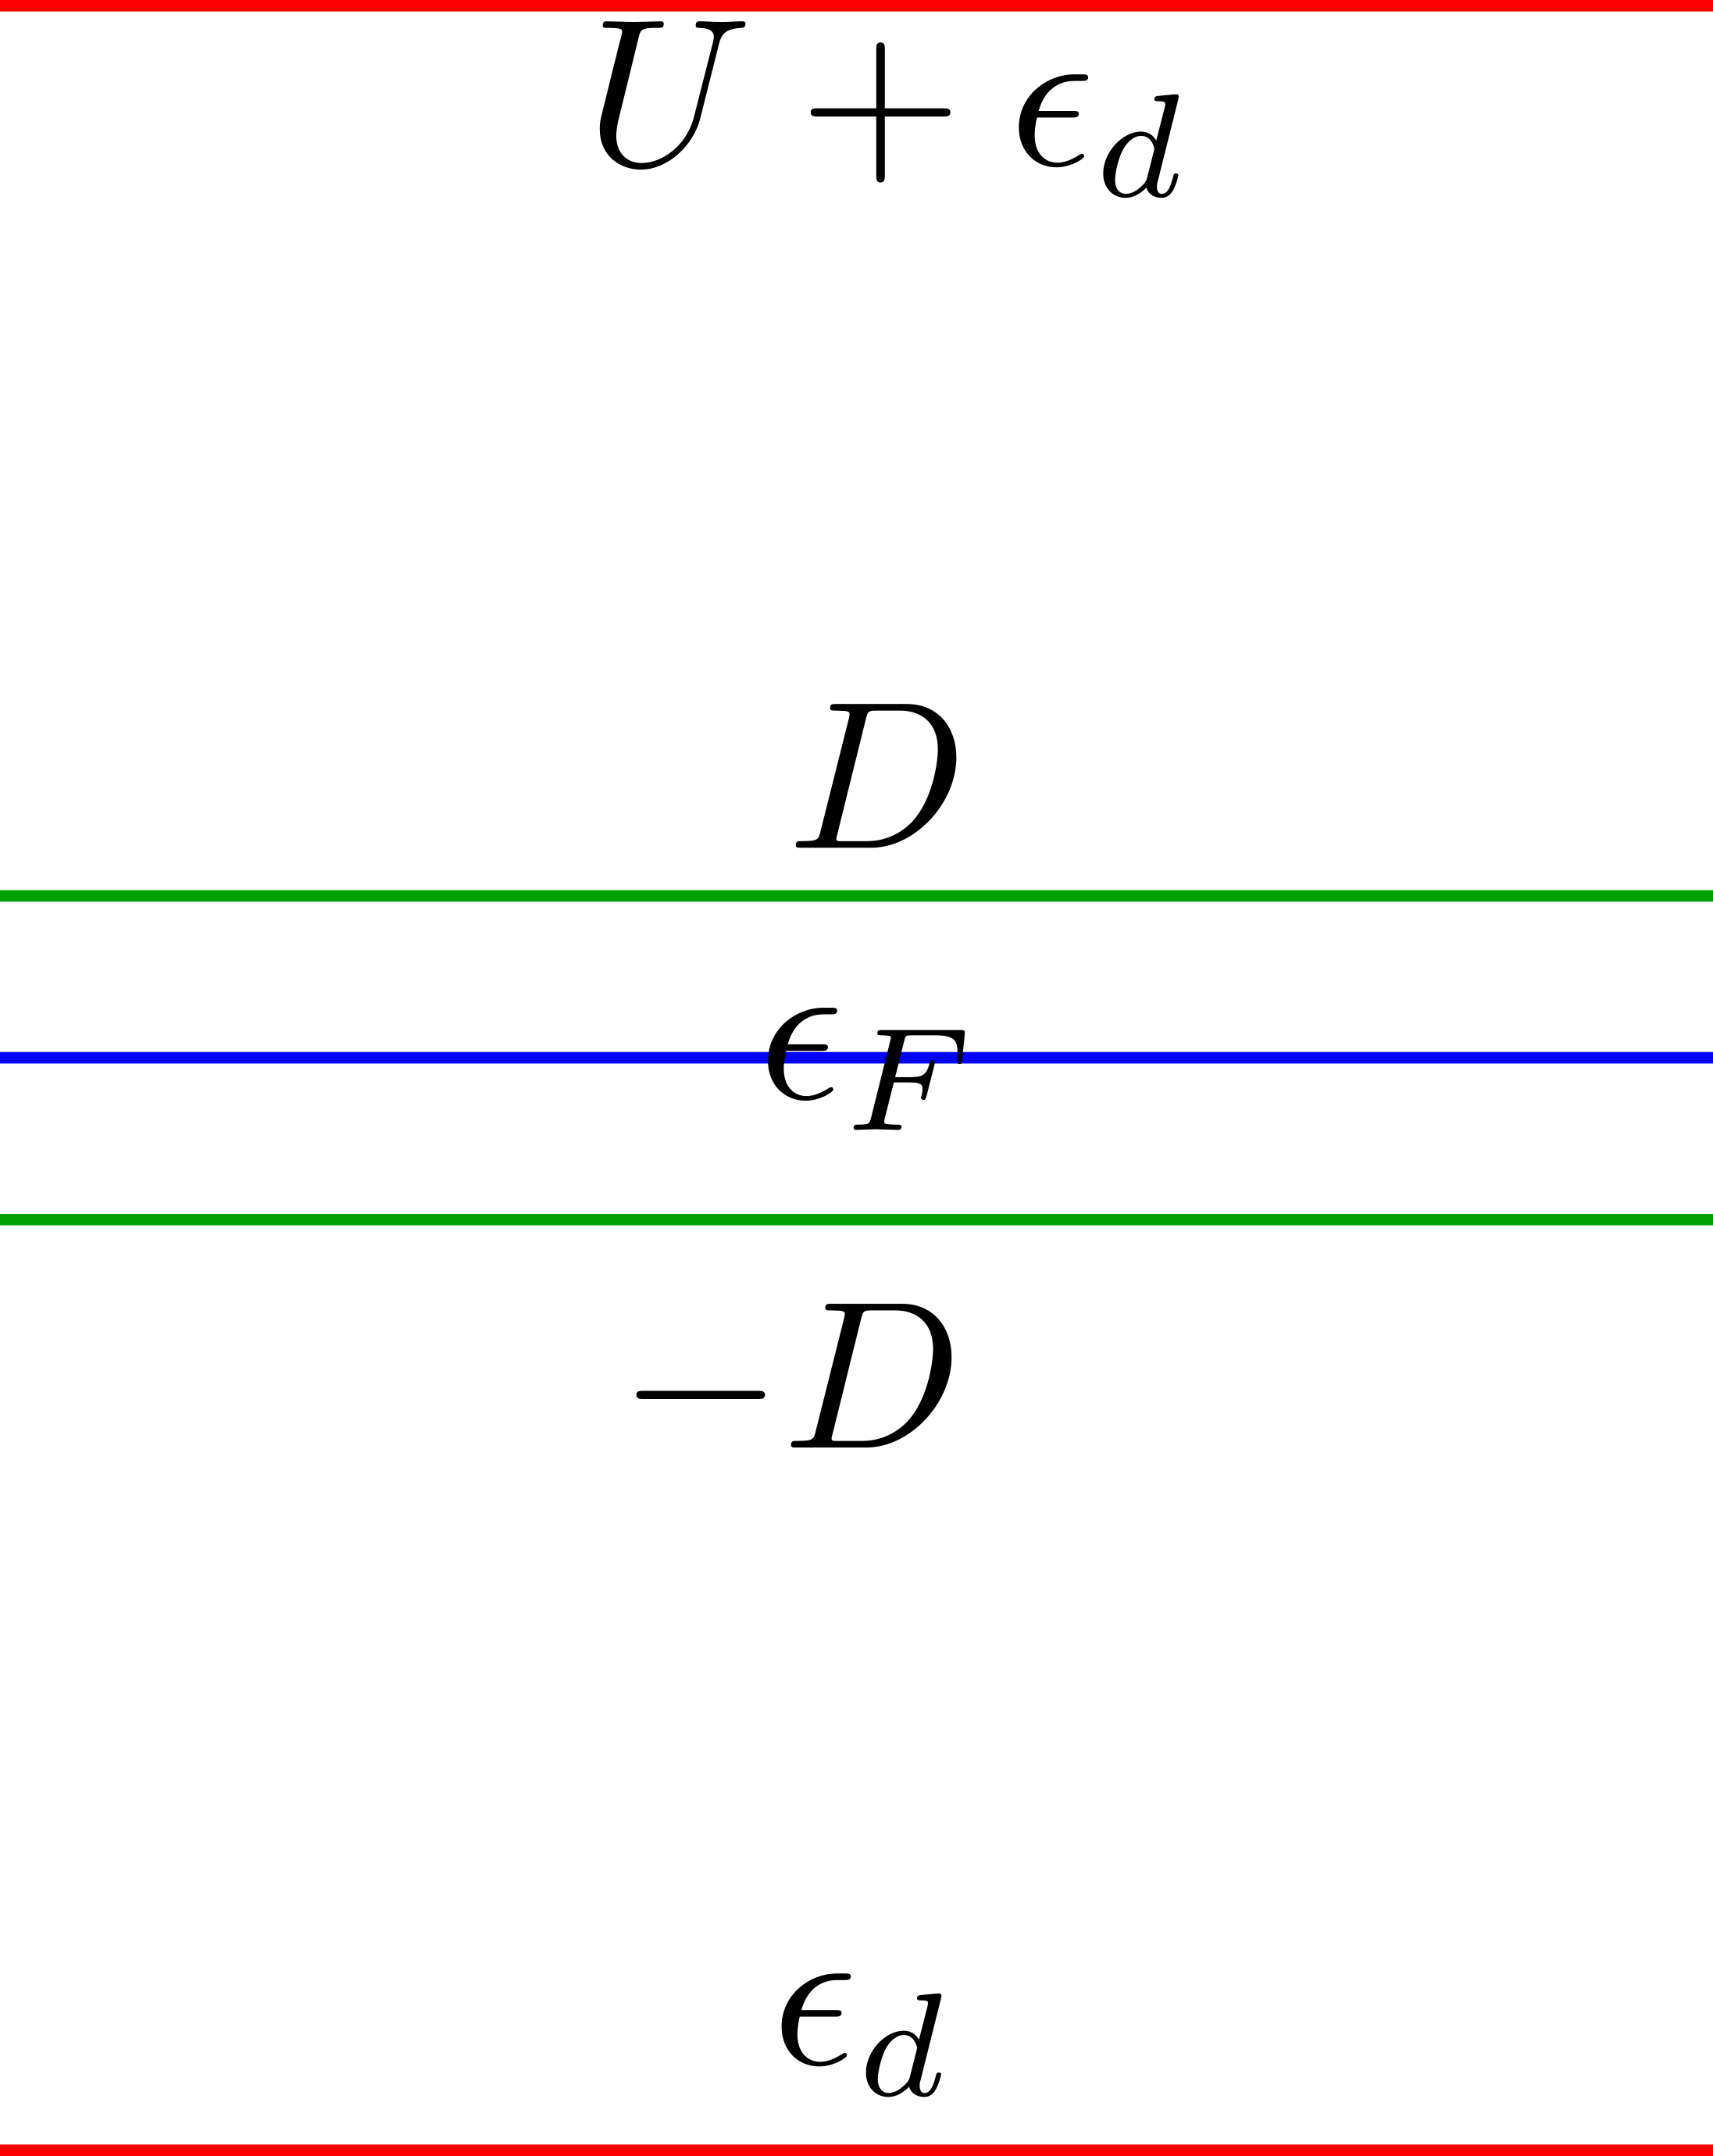
\includegraphics[width=0.6\textwidth]{../figures/anderson.png}
    \caption{\textit{Left}: Both impurity levels far outside the bandwidth. \textit{Right}: Both impurity levels comfortably inside the bandwidth.}
    \label{and}
\end{figure}

The limit where there will be some renormalization is the following.
We are working with the asymmetric Anderson model, that is,\\ \(U + \epsilon_d \gg D \gg |\epsilon_d|,\Delta\).
The total Hamiltonian is
\begin{equation}\begin{aligned}
	H = \sum_{k\sigma} \epsilon_{k\sigma}n_{k\sigma} + \epsilon_d \sum_\sigma n_{d\sigma} + U n_{d\uparrow}n_{d\downarrow} + \sum_{k\sigma}\left(V_{kd} c^\dagger_{k\sigma}c_{d\sigma} + V^*_{kd}c^\dagger_{d\sigma}c_{k\sigma}\right)
\end{aligned}\end{equation}
This means that the doubly-occupied state is decoupled from the conduction band; it cannot hybridize through the \(V_{kd}\) because the virtual transition will involve a huge amount of energy and so it is practically impossible.\\\\
At the first iteration, we will reduce the cut-off from \(D\) to \(D - \delta D\).
The zeroth approximation to this Hamiltonian is
\begin{equation}\begin{aligned}
	H^{(0)} = \sum_{k<D-\delta D, \sigma} \epsilon_{k\sigma}n_{k\sigma} + \epsilon_d \sum_\sigma n_{d\sigma} + \sum_{k<D-\delta D,\sigma}\left(V_{kd} c^\dagger_{k\sigma}c_{d\sigma} + V^*_{kd}c^\dagger_{d\sigma}c_{k\sigma}\right)
\end{aligned}\end{equation}
As is apparent, the zeroth approximation involves completely ignoring the region to be integrated out.
All kinetic energies and actual scatterings are strictly within the smaller region \([-D + \delta D, D - \delta D]\).
The higher approximations  allow these states to make virtual transitions to the band edge states and then come back.
The Hamiltonian term for the virtual excitation in to the upper band edge (with a particle in the intermediate state) is
\begin{equation}\begin{aligned}
H^{(1,p)}_\sigma = \sum_{k\in k^+} \alpha_{k\sigma} c^\dagger_{d\sigma} c_{k\sigma}c^\dagger_{k\sigma} c_{d\sigma}
\end{aligned}\end{equation}
There are two things to note here.
Firstly, \(\alpha_{k\sigma}\) is the probability of such a virtual transition and is found from perturbation theory.
Secondly, the summation \(k^+\) is over the states in \([D-\delta D,D]\).
To calculate \(\alpha_{k\sigma}\), note that such a virtual excitation can take place only from the state \(1_{d\sigma}\).
Therefore, we look at the first order correction to this state under the perturbation \(V_{kd}\).
\begin{equation}\begin{aligned}
\alpha_{k\sigma} = \frac{\bra{1_{d\sigma}}V^*_{kd} c^\dagger_{d\sigma} c_{k\sigma}\ket{k\sigma}\bra{k\sigma}V_{kd}c^\dagger_{k\sigma} c_{d\sigma}\ket{1_{d\sigma}}}{E_{1_d\sigma} - E_{k\sigma}} = \frac{|V_{kd}|^2}{\epsilon_d - \epsilon_k}
\end{aligned}\end{equation}
The analogous term in the same order for the virtual transition to the lower edge consists of a hole in the intermediate state, because the lower edge states are already filled.
This term is of the form
\begin{equation}\begin{aligned}
H^{(1,h)} = \sum_{k\in k^-,\sigma} \beta_{k\sigma} c^\dagger_{k\sigma} c_{d\sigma} c_{k\sigma} c_{d\sigma}^\dagger
\end{aligned}\end{equation}
\(\beta_{k\sigma}\) is calculated similarly, using perturbation theory.

\begin{equation}\begin{aligned}
\beta_{k\sigma} = \frac{\bra{0}V^*_{kd} c_{d\sigma} c^\dagger_{k\sigma}\ket{k\sigma}\bra{k\sigma}V_{kd}c_{k\sigma} c^\dagger_{d\sigma}\ket{0}}{E_0 - E_{k\sigma}} = \frac{|V_{kd}|^2}{\epsilon_k - \epsilon_d}
\end{aligned}\end{equation}
The total first order  correction to the Hamiltonian is of the form
\begin{equation}\begin{aligned}
H^{(1)} = \sum_{k^+,\sigma}\alpha_{k\sigma} T^+_{k\sigma} + \sum_{k^-,\sigma}\beta_{k\sigma} T^-_{k\sigma}
\end{aligned}\end{equation}
\(T^{+,-}\) represent virtual transitions to the upper and lower edges.
Since these terms do not cause any real fluctuations in the impurity sites, they renormalize only the impurity energy \(\epsilon_d\), and not the hybridisation coupling \(V_{kd}\).
To find the renormalization in the site energies \(\epsilon_0\) and \(\epsilon_1\) (and hence in \(\epsilon_d \equiv \epsilon_1 - \epsilon_0\)), note that the term \(T^+\) virtually excites the state \(n_{d\sigma} = 1\), and hence the change in \(\epsilon_{1}\) is
\begin{equation}\begin{aligned}
\delta \epsilon_{1} = \alpha_{k\sigma} = \sum_{k^+}\frac{|V_{kd}|^2}{\epsilon_d - \epsilon_k}
\end{aligned}\end{equation}
We can write this summation in terms of \(\Delta(E) = \pi N(E) V^2(E)\), under the assumption \(\Delta (E) \approx \Delta\) for \(E \in \{-D,D\}\).
\begin{equation}\begin{aligned}
\delta \epsilon_{1} =\sum_{k^+}\frac{|V_{kd}|^2}{\epsilon_d - \epsilon_k} = \int_{D-\delta D}^{D} dE N(E) \frac{|V(E)|^2}{\epsilon_d - E} \approx \frac{\Delta}{\pi}\frac{ |\delta D|}{\epsilon_d - D}
\end{aligned}\end{equation}
The change in \(\epsilon_0\) is
\begin{equation}\begin{aligned}
\delta \epsilon_{0} = \sum_\sigma \beta_{k\sigma} \approx -2\frac{\Delta}{\pi}\frac{ |\delta D|}{\epsilon_d + D}
\end{aligned}\end{equation}
The change in the denominator occurs because in the lower edge, \(\epsilon_k = -D\).
The change in \(\epsilon_d\) is
\begin{equation}\begin{aligned}
	\delta \epsilon_d = \delta \epsilon_1 - \delta \epsilon_0 = \frac{\Delta |\delta D|}{\pi}\left[\frac{1}{\epsilon_d - D} + \frac{2}{\epsilon_d +D}\right] = \frac{\Delta}{\pi}\frac{|\delta D|}{D} = -\frac{\Delta}{\pi}\delta\ln D
\end{aligned}\end{equation}
We assumed \(D \gg \epsilon_d\).
In the limit of infinitesimal change, we get the equation
\begin{equation}\begin{aligned}
	\label{scale_eq}
	\frac{\:\mathrm{d}\epsilon_d}{\:\mathrm{d}\ln D} = -\frac{\Delta}{\pi}
\end{aligned}\end{equation}
If we had allowed the \(\ket{1_{d\sigma}}\) to hybridize with the state \(\ket{2_d}\) (that is, if we had assumed both \(U\) and \(\epsilon_d\) to be \(\ll D\)), then \(\alpha_{k\sigma}\) would have had another term added to it:
\begin{equation}\begin{aligned}
\frac{|V_{kd}|^2}{\epsilon_k - U -\epsilon_d} \approx  \frac{|V|^2}{-D - U -\epsilon_d}
\end{aligned}\end{equation}
\(-(U+\epsilon_d)\) is the change in energy from \(\ket{1_d}\) to \(\ket{2_d}\) and \(-D\) is the energy of the hole created in the process.
The renormalization in \(\epsilon_d\) would then have been
\begin{equation}\begin{aligned}
	\delta \epsilon_d = \frac{\Delta |\delta D|}{\pi}\left(\frac{1}{\epsilon_d - D} - \frac{1}{D + U + \epsilon_d} + \frac{2}{\epsilon_d + D}\right)
\end{aligned}\end{equation}
which is zero in the limit of \(U,|\epsilon_d| \ll D\).
This is the equal renormalization in \(\epsilon_0\) and \(\epsilon_1\) discussed earlier.\\\\
We do not yet know whether \(\Delta\) is a function of the cutoff \(D\).
To find the renormalization of \(\Delta\), we need to find the renormalization of \(V_{kd}\).
Note that the lowest order virtual transitions do not cause any actual charge fluctuation, and hence they do not renormalize \(V_{kd}\).
To see the renormalization of \(V_{kd}\), we need to consider one order higher.
These higher order terms involve transitions within the lower subspace along with virtual transitions into the higher subspaces.
\begin{equation}\begin{aligned}
H^{(2)} = \sum_{k^+,q,\sigma}\alpha_{k\sigma} T^+_{k\sigma}\gamma_{q,k,\sigma}c^\dagger_{d\sigma}c_{q\sigma} + \sum_{k^-,q,\sigma}\beta_{k\sigma} T^-_{k\sigma}\gamma_{q,k,\sigma}c_{d\sigma}c^\dagger_{q\sigma}
\end{aligned}\end{equation}
The \(\gamma_{k\sigma}\) can be calculated as 
\begin{equation}\begin{aligned}
\alpha_{k\sigma}\gamma_{q,k,\sigma} = \frac{\bra{1_{d\sigma}}V^*_{kd} c^\dagger_{d\sigma} c_{k\sigma}\ket{k\sigma}\bra{k\sigma}V_{kd}c^\dagger_{k\sigma} c_{d\sigma}\ket{1_{d\sigma}}\bra{1_{d\sigma}}V_{kd}c_{q\sigma} c^\dagger_{d\sigma}\ket{q\sigma}}{(E_{1_d\sigma} - E_{k\sigma})(E_q - E_k)} \\
= \alpha_{k\sigma}\frac{V_{kd}}{\epsilon_q - \epsilon_k}
\end{aligned}\end{equation}
The renormalization in \(V_{kd}\) is therefore
\begin{equation}\begin{aligned}
\delta V_{kd} = \frac{\Delta}{\pi}\frac{|\delta D|}{\epsilon_d - D}\frac{V_{kd}}{\epsilon_q - \epsilon_k}
\end{aligned}\end{equation}
Close to the band edge, we get
\begin{equation}\begin{aligned}
\delta V = \frac{\Delta}{\pi}\frac{|\delta D|}{\epsilon_d - D}\frac{V}{\epsilon_q - D} \approx \frac{\Delta}{\pi}\frac{|\delta D|}{D^2}V
\end{aligned}\end{equation}
Therefore,
\begin{equation}\begin{aligned}
	\label{mirai2}
	\delta \Delta \sim V\delta V = \frac{\Delta V^2}{\pi D^2}|\delta D| \implies \frac{\:\mathrm{d}\Delta}{\:\mathrm{d}D} \sim \left(\frac{\Delta}{D}\right)^2
\end{aligned}\end{equation}
For \(D \gg \Delta\), this will vanish very quickly.
Hence, in this regime, there is no renormalization of \(\Delta\), and we can take it to be a constant in the renormalization flow.
Integrating eq.~\ref{scale_eq} gives
\begin{equation}\begin{aligned}
\epsilon_d = -\frac{\Delta}{\pi}\ln D + \text{constant}
\end{aligned}\end{equation}
Defining the constant as 
\begin{equation}\begin{aligned}
\text{constant} = \epsilon_d^* + \frac{\Delta}{\pi}\ln \Delta
\end{aligned}\end{equation}
we get
\begin{gather}
\epsilon_d = -\frac{\Delta}{\pi}\ln D +  \epsilon_d^* + \frac{\Delta}{\pi}\ln \Delta \\
\implies \epsilon_d = \epsilon_d^* - \frac{\Delta}{\pi}\ln \frac{D}{\Delta}\label{const}
\end{gather}
This result is in the regime \(U + \epsilon_d \gg D \gg |\epsilon_d|\).
Even if \(U \ll D\) initially, scaling will begin once \(D \sim U\).
Until then, as mentioned previously, both \(\epsilon_1\) and \(\epsilon_0\) will change equally and there won't be any scaling in \(\epsilon_d\).
If we start with \(U \ll D\), under scaling, as \(D\) will decrease, there won't be any renormalization until we reach the point \(D \sim U\).\\\\
Say, as a result of scaling, the bandwidth decreases and \(\epsilon_d\) increases (which it will, as is apparent from the eq.~\ref{const}).
At some point, \(-D \lesssim \epsilon_d\).
At this point, perturbation theory breaks down and we resort to SWT.
We denote this point of the scaling by \(D = -a\widetilde \epsilon_d, a > 1\).
We can then express the SWT coupling constant \(\widetilde J\) by replacing \(\epsilon_d\) with \(\widetilde \epsilon_d\) in eq.~\ref{jexpr}.
For simplicity set \(U = \infty\).
Then,
\begin{equation}\begin{aligned}
	\label{historia}
\widetilde J = -\frac{|V|^2}{\widetilde \epsilon_d} = \frac{a|V|^2}{D}
\end{aligned}\end{equation}
We can then do the poor man's scaling with this coupling.
From eq.~\ref{sol},
\begin{equation}\begin{aligned}
T_K \sim D \sqrt{\widetilde J N(0)^2} \exp\left\{-\frac{1}{2 \widetilde J N(0)^2}\right\} = \sqrt{\Delta D}\exp\left\{-\frac{D}{2\Delta}\right\}\\
\sim D\sqrt{\frac{\Delta}{D}}\exp\left\{\frac{\epsilon_d}{2\Delta}\right\}
\end{aligned}\end{equation}
A different result is obtained if one is in the regime of \(\epsilon_d < -D\).
This is the situation mentioned at the very beginning of the discussion, left of fig.~\ref{and}.
Assuming \(U \rightarrow \infty\) and \(\epsilon_d\) outside the conduction band, we can do a SWT and the \(T_K\) obtained is q.~\ref{sol},
\begin{gather}
    J = -\frac{V^2}{\epsilon_d}\\
    g = J\rho = -\frac{\Delta}{\epsilon_d}\\
    \implies T_K = D\sqrt{\frac{\Delta}{\epsilon_d}}\exp\left\{\frac{\epsilon_d}{2\Delta}\right\}\label{jean2}
\end{gather}
The two forms of the Kondo temperature show that the prefactor is not a universal function; it depends on the starting conditions (the microscopic Hamiltonian from which we start the scaling).
But the universal fact is that in the local moment regime (\(U \rightarrow \infty\)), all physical quantities will involve only one energy scale, \(T_K\).
This \(T_K\) itself might be different based on the starting Hamiltonian.\\\\
For \(\epsilon_d^* \gg \Delta\), the renormalization will stop at \(D \sim \epsilon_d\).
Note that we had assumed \(D \gg \epsilon_d\).
That was the starting condition, that is, \(\epsilon_d\) deep inside the Fermi surface.
During the renormalization, \(D\) will keep on decreasing and \(\epsilon_d\) will continuously increase.
At some value of \(D\), they will become equal and the impurity level will go outside the Fermi surface.
At this point, none of the impurity levels can renormalize any more, because the relevant energy scales are greater than the cutoff.
Hence the renormalization stops at this point.
\begin{figure} 
	\centering 
	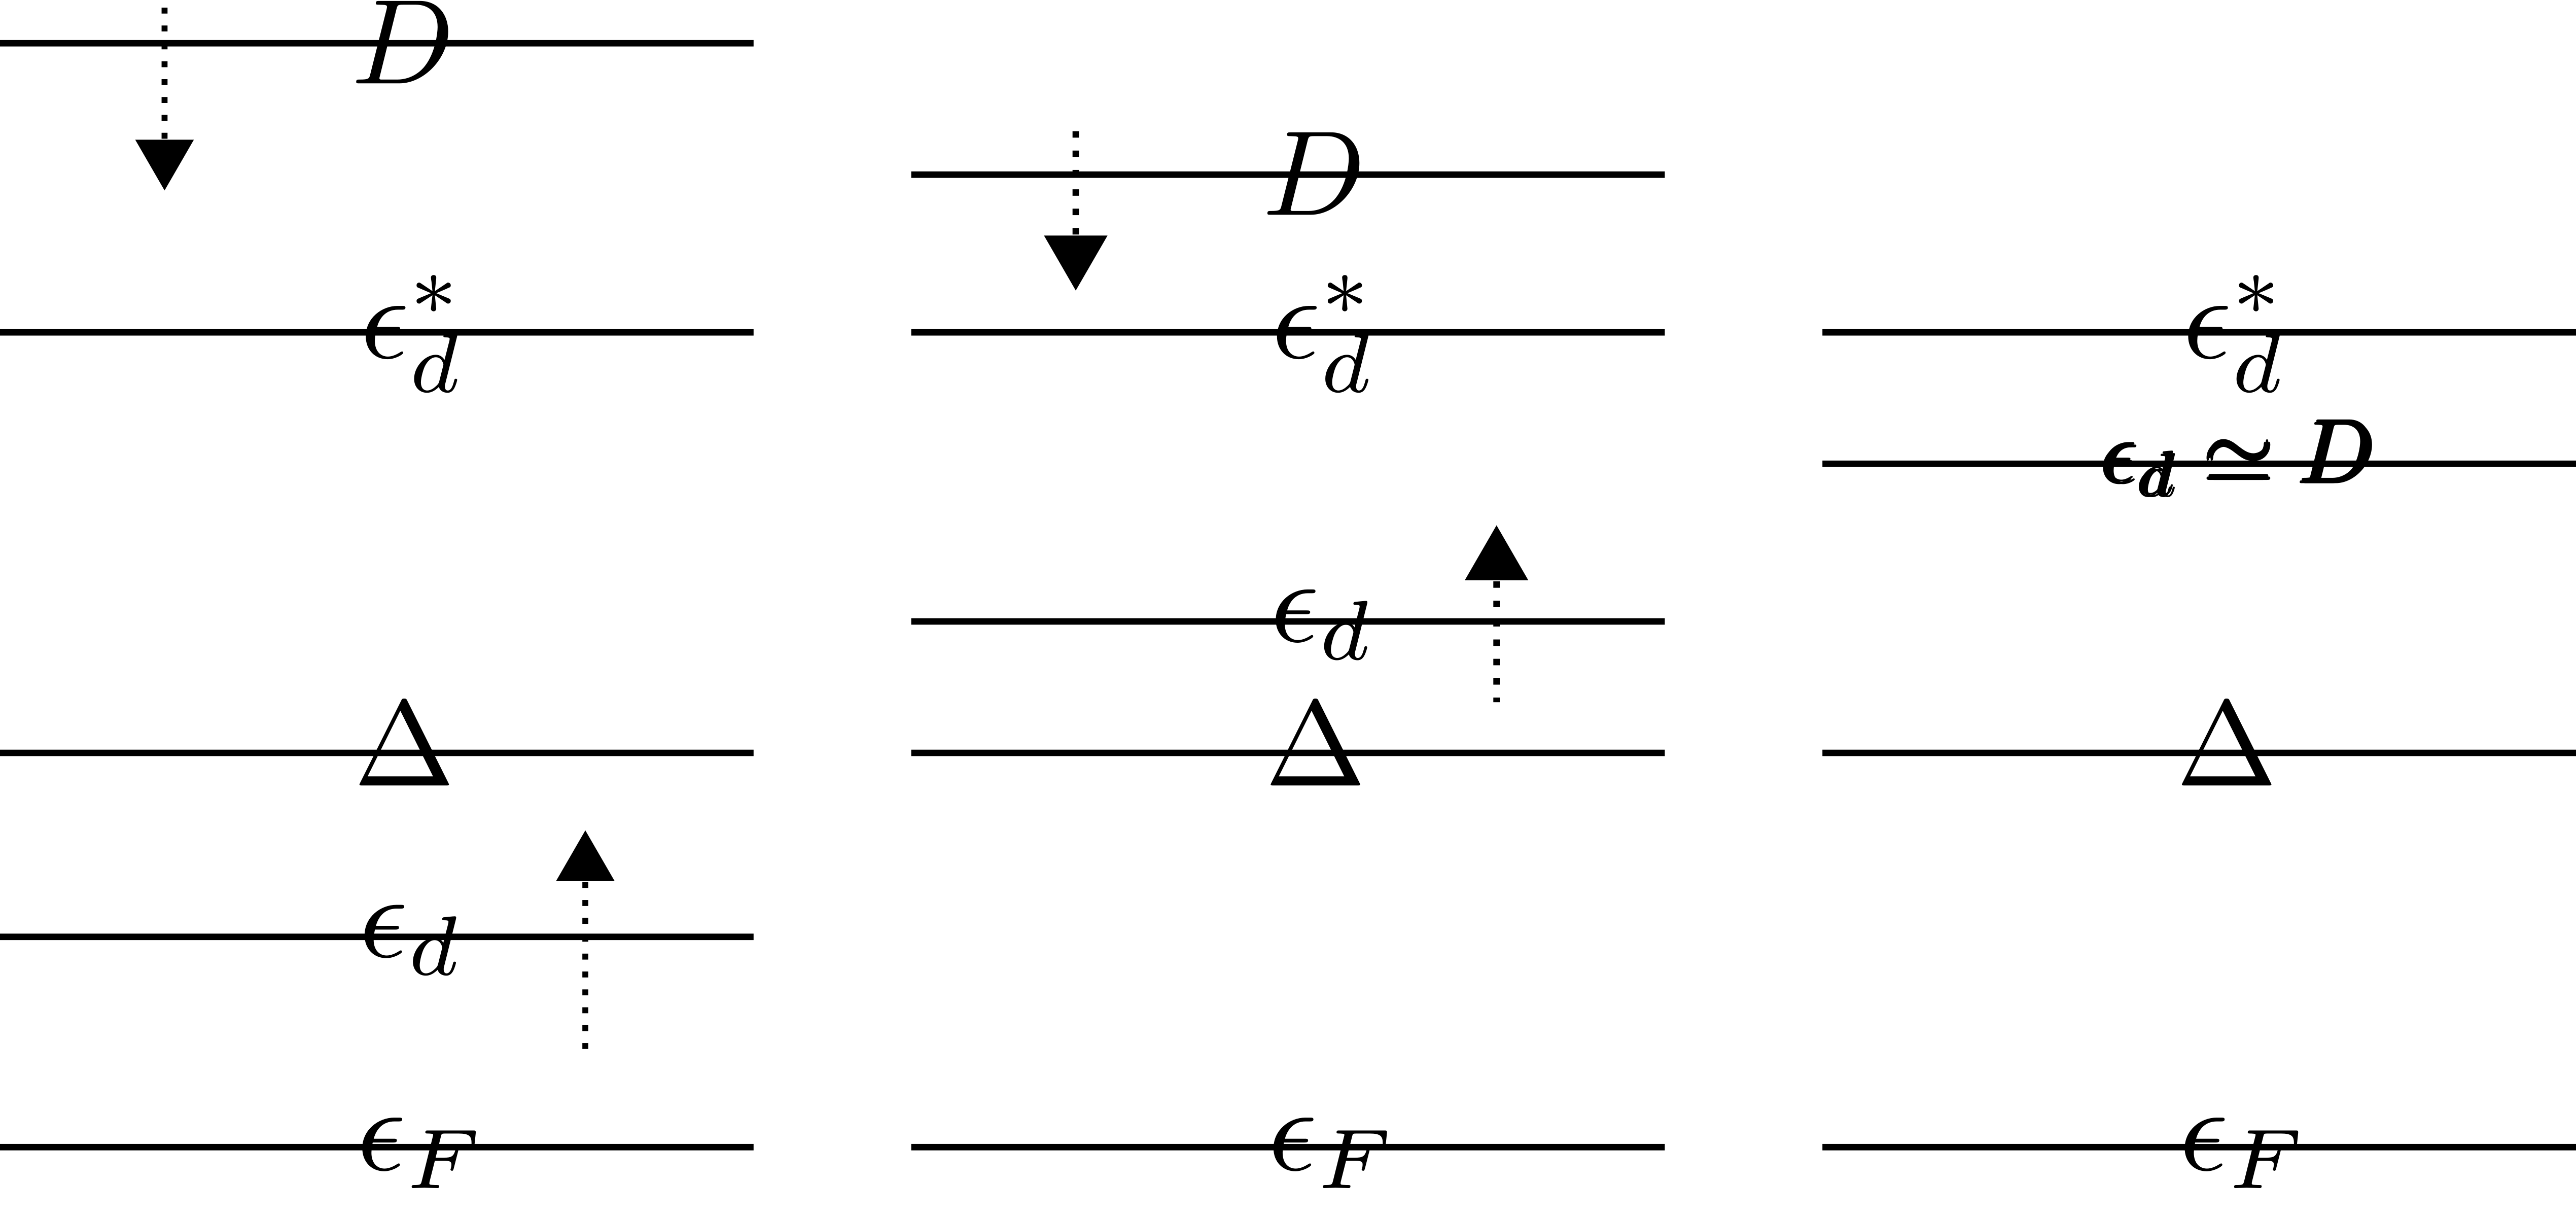
\includegraphics[width=0.6\textwidth]{../figures/full.png}
	\caption{Renormalization in the energy levels when \(\epsilon_d^* \gg \Delta\)}
\end{figure}
This point is given by \(\overline D = a\epsilon_d(\overline D) \equiv \overline \epsilon_d\) where \(a\) is a constant of order unity.
It satisfies the equation
\begin{equation}\begin{aligned}
	\label{eraser}
\overline \epsilon_d = \epsilon_d^* - \frac{\Delta}{\pi}\ln \frac{a\overline \epsilon_d}{\Delta}
\end{aligned}\end{equation}
which is just eq.~\ref{const} with the substitution \(D =a  \overline \epsilon_d\).
In this regime, because \(\epsilon_d \gg \Delta\), we can do a perturbative expansion of the  bare Hamiltonian in terms of \(\frac{\Delta}{\epsilon_d}\).
The susceptibility is
\begin{equation}\begin{aligned}
	\chi_d = \frac{\Delta}{2\pi}\left(\frac{g \mu_B}{\epsilon_d}\right)^2\left[1 + \frac{2\Delta}{\pi \epsilon_d}\ln \frac{\epsilon_d}{D} + ...\right]
\end{aligned}\end{equation}
From the scaling, we know that \(D\) can be decreased to \(\overline D\).
We can hence substitute \(D =a \overline \epsilon_d, \epsilon_d = \overline \epsilon_d\).
With this in mind, the susceptibility becomes
\begin{equation}\begin{aligned}
	\chi_d = \frac{\Delta}{2\pi}\left(\frac{g \mu_B}{\overline\epsilon_d}\right)^2\left[1 + \frac{2\Delta}{\pi \overline\epsilon_d}\ln a + ...\right] \\
	= \frac{\Delta}{2\pi}\left(\frac{g \mu_B}{\overline \epsilon_d}\right)^2\left[1 +\text{O}\left(\frac{2\Delta}{\pi \overline\epsilon_d}\right)\right]
\end{aligned}\end{equation}
where I used the fact that \(\ln a \) will be of order 1.
As we go on decreasing the cutoff, the impurity level will go on moving farther away from the Fermi level, and impurity site will become null occupied: \(\langle  n_d\rangle \approx 0\).
The critical cutoff \(\overline D\) can be associated with a temperature  scale \(k_b \overline T = \overline D\).
At temperatures sufficiently below this temperature (\(T \ll \overline T\)), the susceptibility becomes (again from perturbation theory)
\begin{equation}\begin{aligned}
	\chi_d(T) = \frac{\Delta}{2\pi}\left(\frac{g \mu_B}{\overline \epsilon_d}\right)^2 + \frac{1}{4T}\left[1+\frac{1}{2}\exp\left\{\frac{T^*}{T}\right\}\right]^{-1}
\end{aligned}\end{equation}
For temperatures sufficiently low, which we demarcate by a temperature \(T_{FL}\), the denominator in the second term will be sufficiently large so that we can ignore that term with respect to the first term:
\begin{equation}\begin{aligned}
	T \gg T_{FL} \implies e^\frac{T^*}{T} \gg 1 \implies \left[1+\frac{1}{2}\exp\left\{\frac{T^*}{T}\right\}\right]^{-1} \approx 0 
\end{aligned}\end{equation}
The susceptibility in this low temperature range can thus be written as
\begin{equation}\begin{aligned}
	\label{sakura}
	\chi_d = \frac{\Delta}{2\pi}\left(\frac{g \mu_B}{\overline \epsilon_d}\right)^2
\end{aligned}\end{equation}
This is analogous to the  result obtained in eq.~\ref{mimp}, from the mean field version of the Fermi liquid theory, and also obtained from a renormalized perturbation theory of Anderson model.
To see how, note that since we are in the limit \(\langle  n_d\rangle = 0\), the onsite repulsion term \(U\) can be dropped because there is no probability of double occupation.
Eq.~\ref{mimp} then becomes
\begin{equation}\begin{aligned}
	\label{sasuke}
\chi_d = \frac{g^2 \mu_B^2}{2} \rho_d(0) = \frac{g^2 \mu_B^2}{2} \frac{\Delta}{\pi}\frac{1}{\overline \epsilon_d^2 + \Delta^2}
\end{aligned}\end{equation}
Next note that we had assumed at the beginning that \(\epsilon_d^* \gg \Delta\).
We need to find the relative order difference between \(\overline \epsilon_d\) and \(\Delta\).
From eq.~\ref{eraser}, we can drop the \(\pi\) and \(a\) because they are of order 1.
\begin{equation}\begin{aligned}
\overline \epsilon_d = \epsilon_d^* - \Delta \ln \frac{\overline \epsilon_d}{\Delta}
\end{aligned}\end{equation}
Dividing through by \(\Delta\) and defining \(x_1 = \frac{\overline \epsilon_d}{\Delta}, x_2 = \frac{\epsilon_d^*}{\Delta}\), we get
\begin{equation}\begin{aligned}
x_1 + \ln x_1 = x_2
\end{aligned}\end{equation}
Since \(O(\ln x_1) \leq O(x_1)\), we can write
\begin{gather}
O(x_1) = O(x_2)\\
\implies O\left(\frac{\overline \epsilon_d}{\Delta}\right) = O\left(\frac{\epsilon_d^*}{\Delta}\right)\\
\implies O\left(\overline \epsilon_d\right) = O\left(\epsilon_d^*\right)\\
\end{gather}
Since \(\overline \epsilon_d\) and \(\epsilon_d^*\) are of the same order, we can say:
\begin{equation}\begin{aligned}
\epsilon_d^* \gg \Delta \implies \overline \epsilon_d \gg \Delta
\end{aligned}\end{equation}
Applying this to eq.~\ref{sasuke} means
\begin{equation}\begin{aligned}
\chi_d \approx \frac{g^2 \mu_B^2}{2} \frac{\Delta}{\pi}\frac{1}{\overline \epsilon_d^2}
\end{aligned}\end{equation}
which is the same as eq.~\ref{sakura}.
This tells us that scaling all the way down to very low temperatures in regime \(\epsilon_d^* \gg \Delta\) brings us into a Fermi liquid state, characterized by a temperature-independent susceptibility (as is standard in a Fermi liquid).
The crossovers can be seen by looking at the variation of the Curie constant \(\chi T\).\\\\
Since the susceptibility is proportional to the magnetic moment, presence of degeneracy will reduce this moment because the probability of occupying the states will decrease.
As a result, the Curie constant is also a measure of the effective degeneracy of the impurity orbital.
At very high temperatures \(T \gg U,\epsilon_d\), all the impurity levels \(0,\epsilon_d\) and \(2\epsilon_d + U\) will become degenerate on energy scales of the order of \(k_B T\).
As a result, the Curie constant is approximately \(\frac{1}{8}\) in this range.
The impurity occupancy is \(n_d = 1\), because there are 4 degenerate states and the average number of electrons on them is 1.
At lower temperatures \(U \gg T \gg T^*\), the degeneracy gets lowered; now, only the vacant and single-occupied states are degenerate.
Here the Curie constant is \(\frac{1}{6}\).
In this case, the average occupancy is \(n_d = \frac{0+1+1}{3} = \frac{2}{3}\).
At still lower temperatures, we saw that the impurity becomes vacant and \(n_d = 0\).
The Curie constant becomes linear in temperature, going down to 0.
More formally,
\begin{equation}\begin{aligned}
	\label{suscep}
	m = \frac{1}{\beta}\frac{\partial{\ln Z}}{\partial{B}} \implies \chi = \lim_{B \to 0}\frac{\partial{m}}{\partial{B}} = \lim_{B \to 0}\frac{1}{Z^2\beta}\left[Z\frac{\partial^2 Z}{\partial B^2} - \left(\frac{\partial{Z}}{\partial{B}}\right)^2\right]
\end{aligned}\end{equation}
For the case of four-fold degeneracy, all the states can be assumed to be at zero energy.
Then, under a magnetic field B (\(h=\frac{g\mu_B}{2}B\)), the partition function is
\begin{gather}
	Z = 1 + \exp\left\{\beta h\right\} + \exp\left\{-\beta h\right\} + 1 = 2\left(1+\cosh \beta h\right)\\
	\implies \frac{\partial{Z}}{\partial{B}} = g \mu_B \beta \sinh \beta h\\
\implies \frac{\partial^2 Z}{\partial B^2} = \frac{1}{2}\left(g \mu_B\right)^2 \beta^2 \cosh \beta h
\end{gather}
Since \(\lim_{h \to 0} \sinh \beta h = 0\) and \(\lim_{h \to 0} \cosh \beta h = 1\), we get
\begin{gather}
\chi = \frac{\beta g^2 \mu_B^2}{2 Z(h=0)}
\end{gather}
Setting \(g \mu_B = k_B = 1\), we get
\begin{equation}\begin{aligned}
	\label{suscdeg}
\chi T =\frac{1}{2\mathcal{D}}
\end{aligned}\end{equation}
where \(Z(h=0) = 2 + 2 = 4 = \mathcal{D}\) is the degeneracy.
\\\\
Similarly, for the triplet case (\(\epsilon_d\) and 0 are degenerate while \(U \gg T\)), the doubly occupied case is essentially cut off from the available states, so \(Z = 1 + 2\cosh \beta h\).
The proof again goes through similarly.
But this time, we have \(Z(h=0) = 1 + 2 = 3 = \mathcal{D}\).\\\\
For \(\epsilon_d = k_B T^* > k_B T\) such that \(k_B T^* \gg \Delta\), we can find the magnetic moment in a perturbative fashion.
At the zeroth order, we can neglect the hybridisation \(\Delta\).
Then,
\begin{equation}\begin{aligned}
	m^{(0)} = \frac{1}{\beta}\frac{\partial{\ln Z(h)}}{\partial{B}}
\end{aligned}\end{equation}
where
\begin{equation}\begin{aligned}
	Z(h) = 1 + e^{-\beta\left(k_B T^* -h\right)}+ e^{-\beta\left(k_B T^* +h\right)} = 1 + e^{-\frac{\beta}{\beta^*}}2\cosh \beta h
\end{aligned}\end{equation}
Therefore,
\begin{equation}\begin{aligned}
\chi^{(0)} = \lim_{h \to 0} \frac{1}{\beta Z}\frac{\partial^2 Z}{\partial B^2} = \lim_{h \to 0} \frac{g^2 \mu_B^2}{4 \beta Z}\frac{\partial^2 Z}{\partial h^2} = \frac{g^2 \mu_B^2}{4}\beta \frac{2e^{-\frac{\beta}{\beta^*}}}{1 + 2e^{-\frac{\beta}{\beta^*}}}
\end{aligned}\end{equation}
Again setting \(g \mu_B = k_B = 1\), we get,
\begin{equation}\begin{aligned}
\chi^{(0)} = \frac{1}{4 T} \frac{2e^{-\frac{\beta}{\beta^*}}}{1 + 2e^{-\frac{\beta}{\beta^*}}} = \frac{1}{4 T} \frac{2}{e^{\frac{\beta}{\beta^*}} + 2} 
\end{aligned}\end{equation}
As a first approximation, we can include the hybridisation by using the expression for the average number of spin up or spin down impurity as obtained from the non-interacting treatment, eq.~\ref{total}
\begin{equation}\begin{aligned}
	m^{(1)} =\frac{g \mu_B}{2}\left( n_\uparrow - n_\downarrow\right) = \frac{g \mu_B}{2\pi}\left[\tan^{-1}\frac{\Delta}{k_B T^* - h} - \tan^{-1}\frac{\Delta}{k_B T^* + h}\right]
\end{aligned}\end{equation}
Since \(\Delta \ll T^*\), we can expand the arctan in a Taylor series.
Up to first order, we get
\begin{equation}\begin{aligned}
	m^{(1)} = \frac{g \mu_B}{2\pi}\left[\frac{\Delta}{k_B T^* - h} - \frac{\Delta}{k_B T^* + h}\right] = \frac{g \mu_B \Delta}{\pi}\frac{h}{k_B \left(T^*\right)^2 - h^2}
\end{aligned}\end{equation}
Differentiating with \(B\) gives
\begin{equation}\begin{aligned}
	\chi^{(1)} = \lim_{h \to 0} \frac{\partial{m^{(1)}}}{\partial{B}} = \frac{g^2\mu_B^2}{2}\frac{\Delta}{\pi}\frac{1}{k_B^2 {T^*}^2} = \frac{\Delta}{2\pi {T^*}^2}
\end{aligned}\end{equation}
Combining the zeroth and first order terms, the susceptibility in the regime \(T \lesssim T^*\) is
\begin{equation}\begin{aligned}
\chi = \frac{1}{4 T} \frac{2}{e^{\frac{\beta}{\beta^*}} + 2}  + \frac{\Delta}{2\pi {T^*}^2}
\end{aligned}\end{equation}
Below some temperature \(T_\text{FL} \ll T^*\), the susceptibility reduces to
\begin{gather}
\chi \approx \frac{1}{4 T} \frac{2}{e^{\frac{\beta}{\beta^*}}} + \frac{\Delta}{2\pi {T^*}^2} \approx\frac{\Delta}{2\pi {T^*}^2}\\
\implies \chi T \propto T
\end{gather}
We can now visualize the various phases as the temperature is changed.
For \(T \gg U,\epsilon_d\), all the four states states \(\ket{0},\ket{\uparrow},\ket{\downarrow},\ket{2}\) are degenerate (\(\mathcal D = 4\)), the average occupancy is \(\langle  n_d\rangle = \frac{0+1+1+2}{4}=1\) and the effective Curie constant is \(\frac{1}{2\mathcal D} = \frac{1}{8}\).
At lower temperatures \(U \gg T \gg T^*\), the level \(\ket{2}\) is disconnected from the conduction band and the three remaining states are now degenerate (\(\mathcal D = 3\)).
The average occupancy becomes \(\frac{0+1+1}{3} = \frac{2}{3}\) and the effective Curie constant is now \(\frac{1}{2\times 3} = \frac{1}{6}\).
At still lower temperatures \(T^* \gg T\), the singly-occupied levels become disconnected and thee impurity occupancy becomes 0.
The effective Curie constant in this regime is linear in \(T\).
\begin{center}
\begin{minipage}{50pt}
	\(n_d = 1\)\\\(\chi T \sim \frac{1}{8}\)\\\(T\gg U\)
\end{minipage}
\hspace*{20pt}\(\Longrightarrow\)\hspace*{20pt}
\begin{minipage}{50pt}
	\(n_d = \frac{2}{3}\)\\\(\chi T \sim \frac{1}{6}\)\\\(T\gg T^*\)
\end{minipage}
\hspace*{20pt}\(\Longrightarrow\)\hspace*{20pt}
\begin{minipage}{50pt}
	\(n_d = 0\)\\\(\chi T \sim T\)\\\(T\ll T^*\)
\end{minipage}
\end{center}
Next we consider the mixed valence regime, described by \(|\epsilon_d^*| < \Delta\).
It is clear that since the impurity level is within an interval of the hybridisation from the Fermi surface, the charge fluctuations can cause transitions between the various states of the impurity.
This means that the occupation number of the impurity site is not a good quantum number in this regime, and the average number of impurity electrons will be fractional.
This definition is a bit arbitrary because any observed sample will display an eigenstate in which the impurity states have contributions from both \(\langle  n_d\rangle=0\) and \(\langle  n_d\rangle=1\), so any sample will be mixed in that sense.
However, if we are not in the mixed valence regime (\(|\epsilon_d| \gg \Delta\)), then the contribution from any one state will far outweigh the other.
If \(\epsilon_d > 0\), then the impurity level is far above the Fermi level and it will most probably not be occupied and the majority of the contribution will come from \(\langle  n_d\rangle = 0\).
Similarly, if \(\epsilon_d < 0\), then the impurity level is far below the Fermi level and the average occupation will be close to 1.
The regime of mixed valence is one in which these two contributions are comparable.
\\\\
\begin{figure}
	\centering
	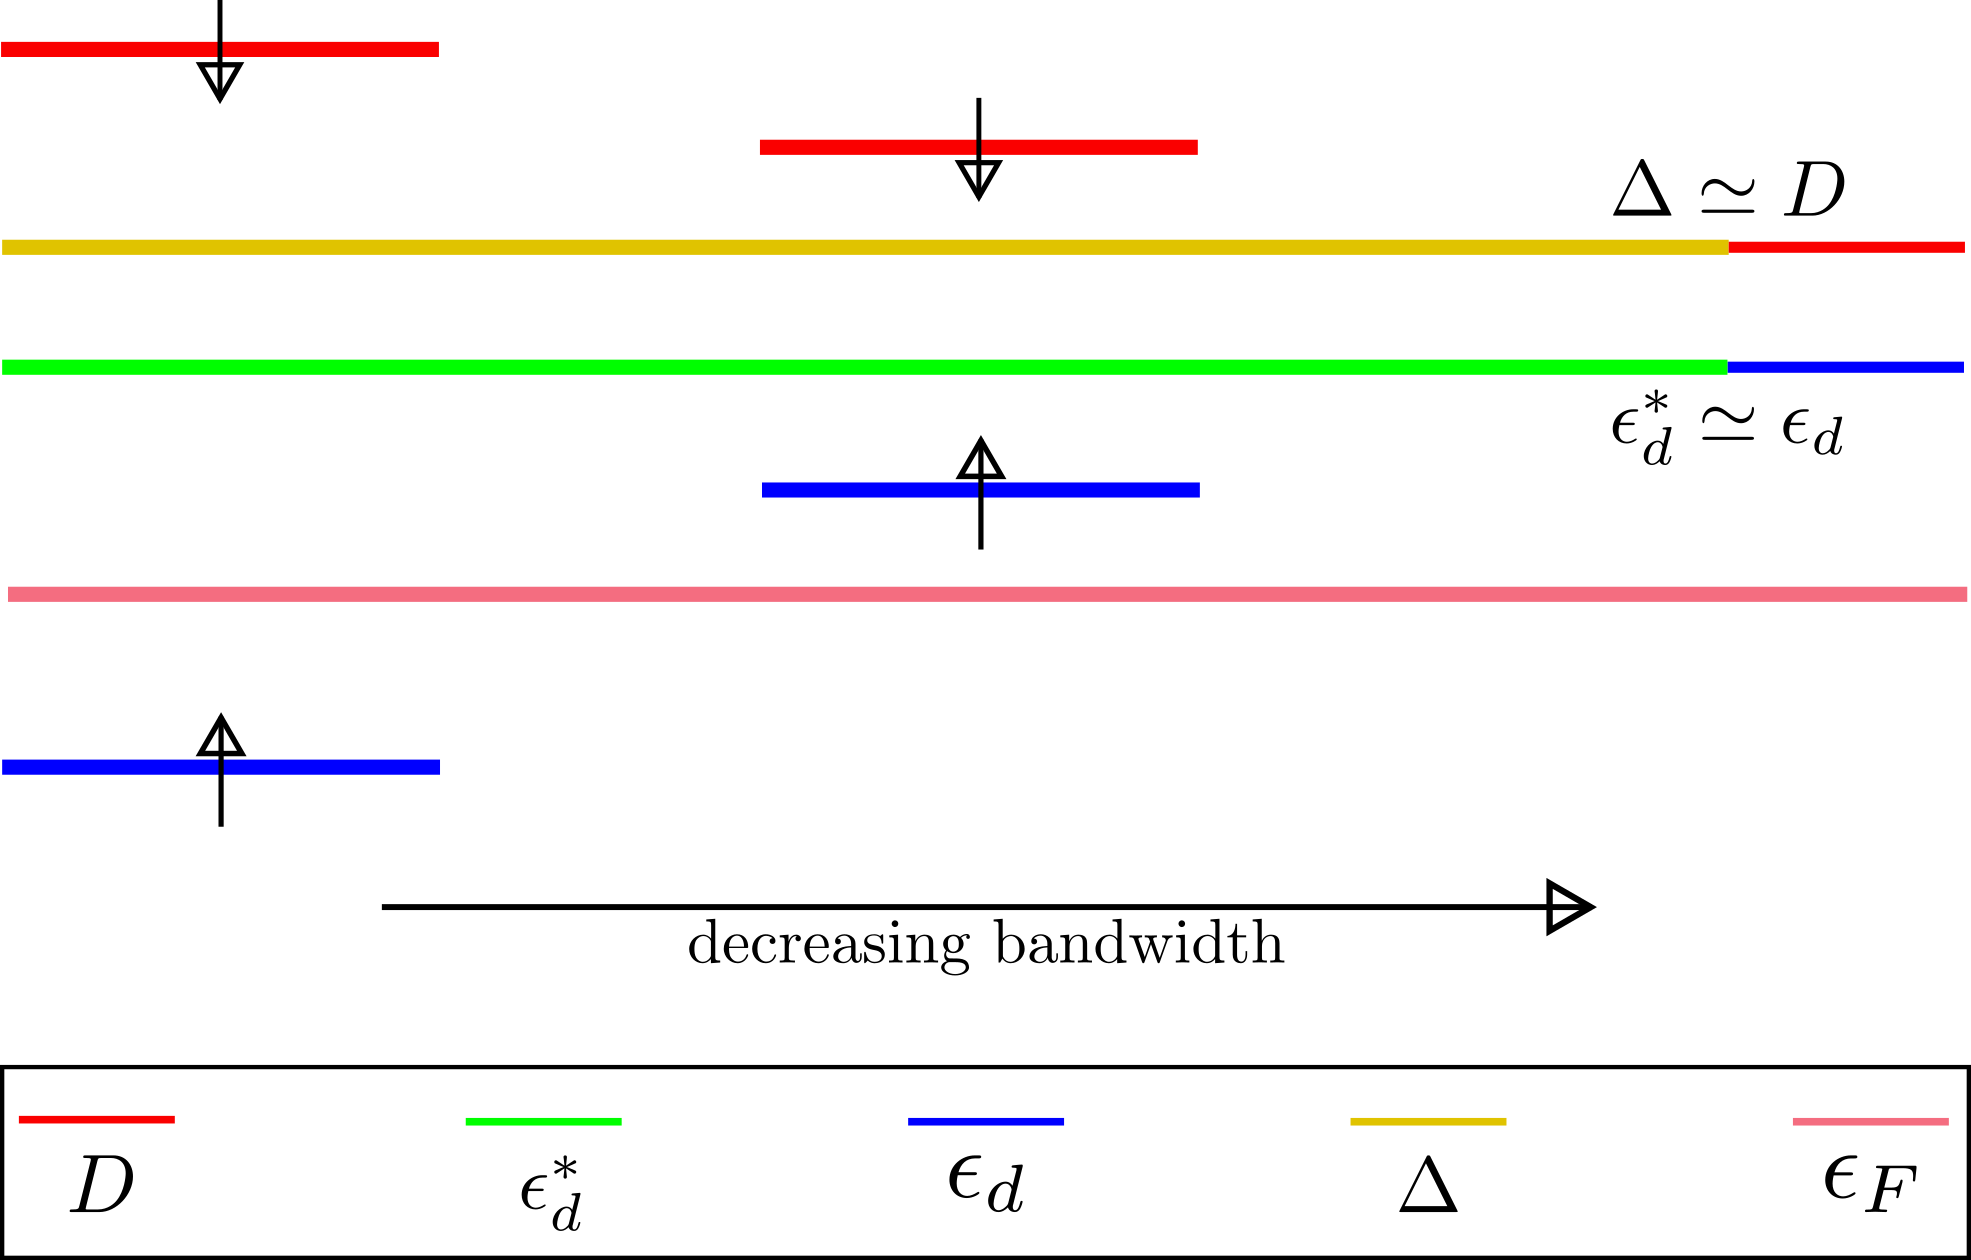
\includegraphics[width=0.6\textwidth]{../figures/mixed.png}
	\caption{Renormalization in energy levels when \(|\epsilon_d^*| \lesssim \Delta\)}
\end{figure}
Since we have \(|\epsilon_d^*| \lesssim \Delta\), as we renormalize, the decreasing cutoff will first match \(\Delta\) or \(k_B T\), whichever is greater.
From eq.~\ref{mirai2}, we know that if \(D\) comes close to \(\Delta\), our analysis will break down because we can no longer ignore that term.
Since that term represents the broadening of the impurity level, this same broadening can also be brought about by the thermal fluctuations which are of the scale \(k_B T\).
This means that real valence fluctuations will now renormalize the potential \(V_{kd}\).
Hence, our analysis will stop at \(D = \text{max}\left\{\Delta, k_B T\right\}\).
For the simpler situation in which \(T = 0\), the renormalization will stop at \(D = \Delta\).
From eq.~\ref{const}, putting \(D = \Delta\), we get
\begin{equation}\begin{aligned}
	\left(\epsilon_d\right)_\text{MV} = \epsilon_d^*
\end{aligned}\end{equation}
This is the renormalized impurity level in the mixed valence regime.
A characteristic feature of this regime is that the charge fluctuations can be thermally excited.
This can be seen as follows.
The probability of  a transition from, say, \(\ket{n_d = 0}\) to \(\ket{n_d = 1}\) is
\begin{equation}\begin{aligned}
\sim \frac{k_B T}{\epsilon_d}
\end{aligned}\end{equation}
Assuming the thermal fluctuations are more or less of the order \(\Delta\), for \(\epsilon_d \gg \Delta\), this transition will not be possible.
However, in the mixed valence regime, because \(\epsilon_d \sim \Delta\), these excitations do occur.
These fluctuations, as well as the ones from the hybridisation with the conduction band, are responsible for the mixing of the singly-occupied and null-occupied states.\\\\
The crossovers in the mixed valence regime are as follows.
Similar to the previous case, at high and intermediate temperatures, we have \(n_d = 1\) and \(n_d = \frac{2}{3}\) respectively.
However, while the triplet degeneracy lasted upto \(T \sim T^*\) in the previous case, here it continues up to \(T \sim \Delta\) because that is where the scaling breaks down.
That is, \(T = \Delta\) is the point where we can no longer ignore the renormalization in \(V\) and it begins to increase with scaling.
Beyond this point, the impurity occupation remains fractional and not much else can be said.
\begin{center}
\begin{minipage}{50pt}
	\(n_d = 1\)\\\(\chi T = \frac{1}{8}\)\\\(T\gg U\)
\end{minipage}
\hspace*{20pt}\(\Longrightarrow\)\hspace*{20pt}
\begin{minipage}{50pt}
	\(n_d = \frac{2}{3}\)\\\(\chi T = \frac{1}{6}\)\\\(T\gg \Delta\)
\end{minipage}
\hspace*{20pt}\(\Longrightarrow\)\hspace*{20pt}
\begin{minipage}{50pt}
	\(n_d = \text{fractional}\)\\\(\chi T \propto T\)\\\(T\ll \Delta\)
\end{minipage}
\end{center}
For \(\epsilon_d^* \ll -\Delta\), the scaling will stop when the impurity level again goes out of the Fermi surface.
But this time, it goes out from below.
This again decouples the singly-occupied state from the conduction band and the scaling stops.
This happens at say \(\widetilde D = -\widetilde {\epsilon_d} = \widetilde {T}\).
Since the singly-occupied impurity level is now well below \(-D\), we have \(\langle  n_d\rangle = 1\) and we are comfortably in the Kondo limit and the SWT and a consequent poor man's scaling can be performed, which will give eqs.~\ref{historia} through \ref{jean2}.
The resulf of the Schrieffer-Wolff transformation is a Hamiltonian that couples the impurity to the conduction electrons only through their spins; their is no charge fluctuation.
At high temperatures \(T \gg T_K\), the impurity is essentially decoupled and we get a susceptibility of the form eq.~\ref{suscdeg}, but with a degeneracy of 2.
To go to lower temperatures, we can do a Poor Man's scaling which suggests that the Hamiltonian at \(T\ll T_K\) is one with a large coupling between the impurity and the conduction electrons.
\begin{center}
\begin{minipage}{50pt}
	\(n_d = 1\)\\\(\chi T = \frac{1}{8}\)\(T\gg U\)
\end{minipage}
\hspace*{20pt}\(\Longrightarrow\)\hspace*{20pt}
\begin{minipage}{50pt}
	\(n_d = \frac{2}{3}\)\\\(\chi T = \frac{1}{6}\)\\\(T\gg \widetilde T\)
\end{minipage}
\hspace*{20pt}\(\Longrightarrow\)\hspace*{20pt}
\begin{minipage}{50pt}
	\(n_d = 1\)\\\(\chi T= \frac{1}{4}\)\\\(T\ll \widetilde T\)
\end{minipage}
\hspace*{20pt}\(\Longrightarrow\)\hspace*{20pt}
\begin{minipage}{50pt}
	\(n_d = 1\)\\\(\chi T \propto T\)\\\(T\ll \widetilde T_K\)
\end{minipage}
\end{center}
\begin{figure}
	\centering 
	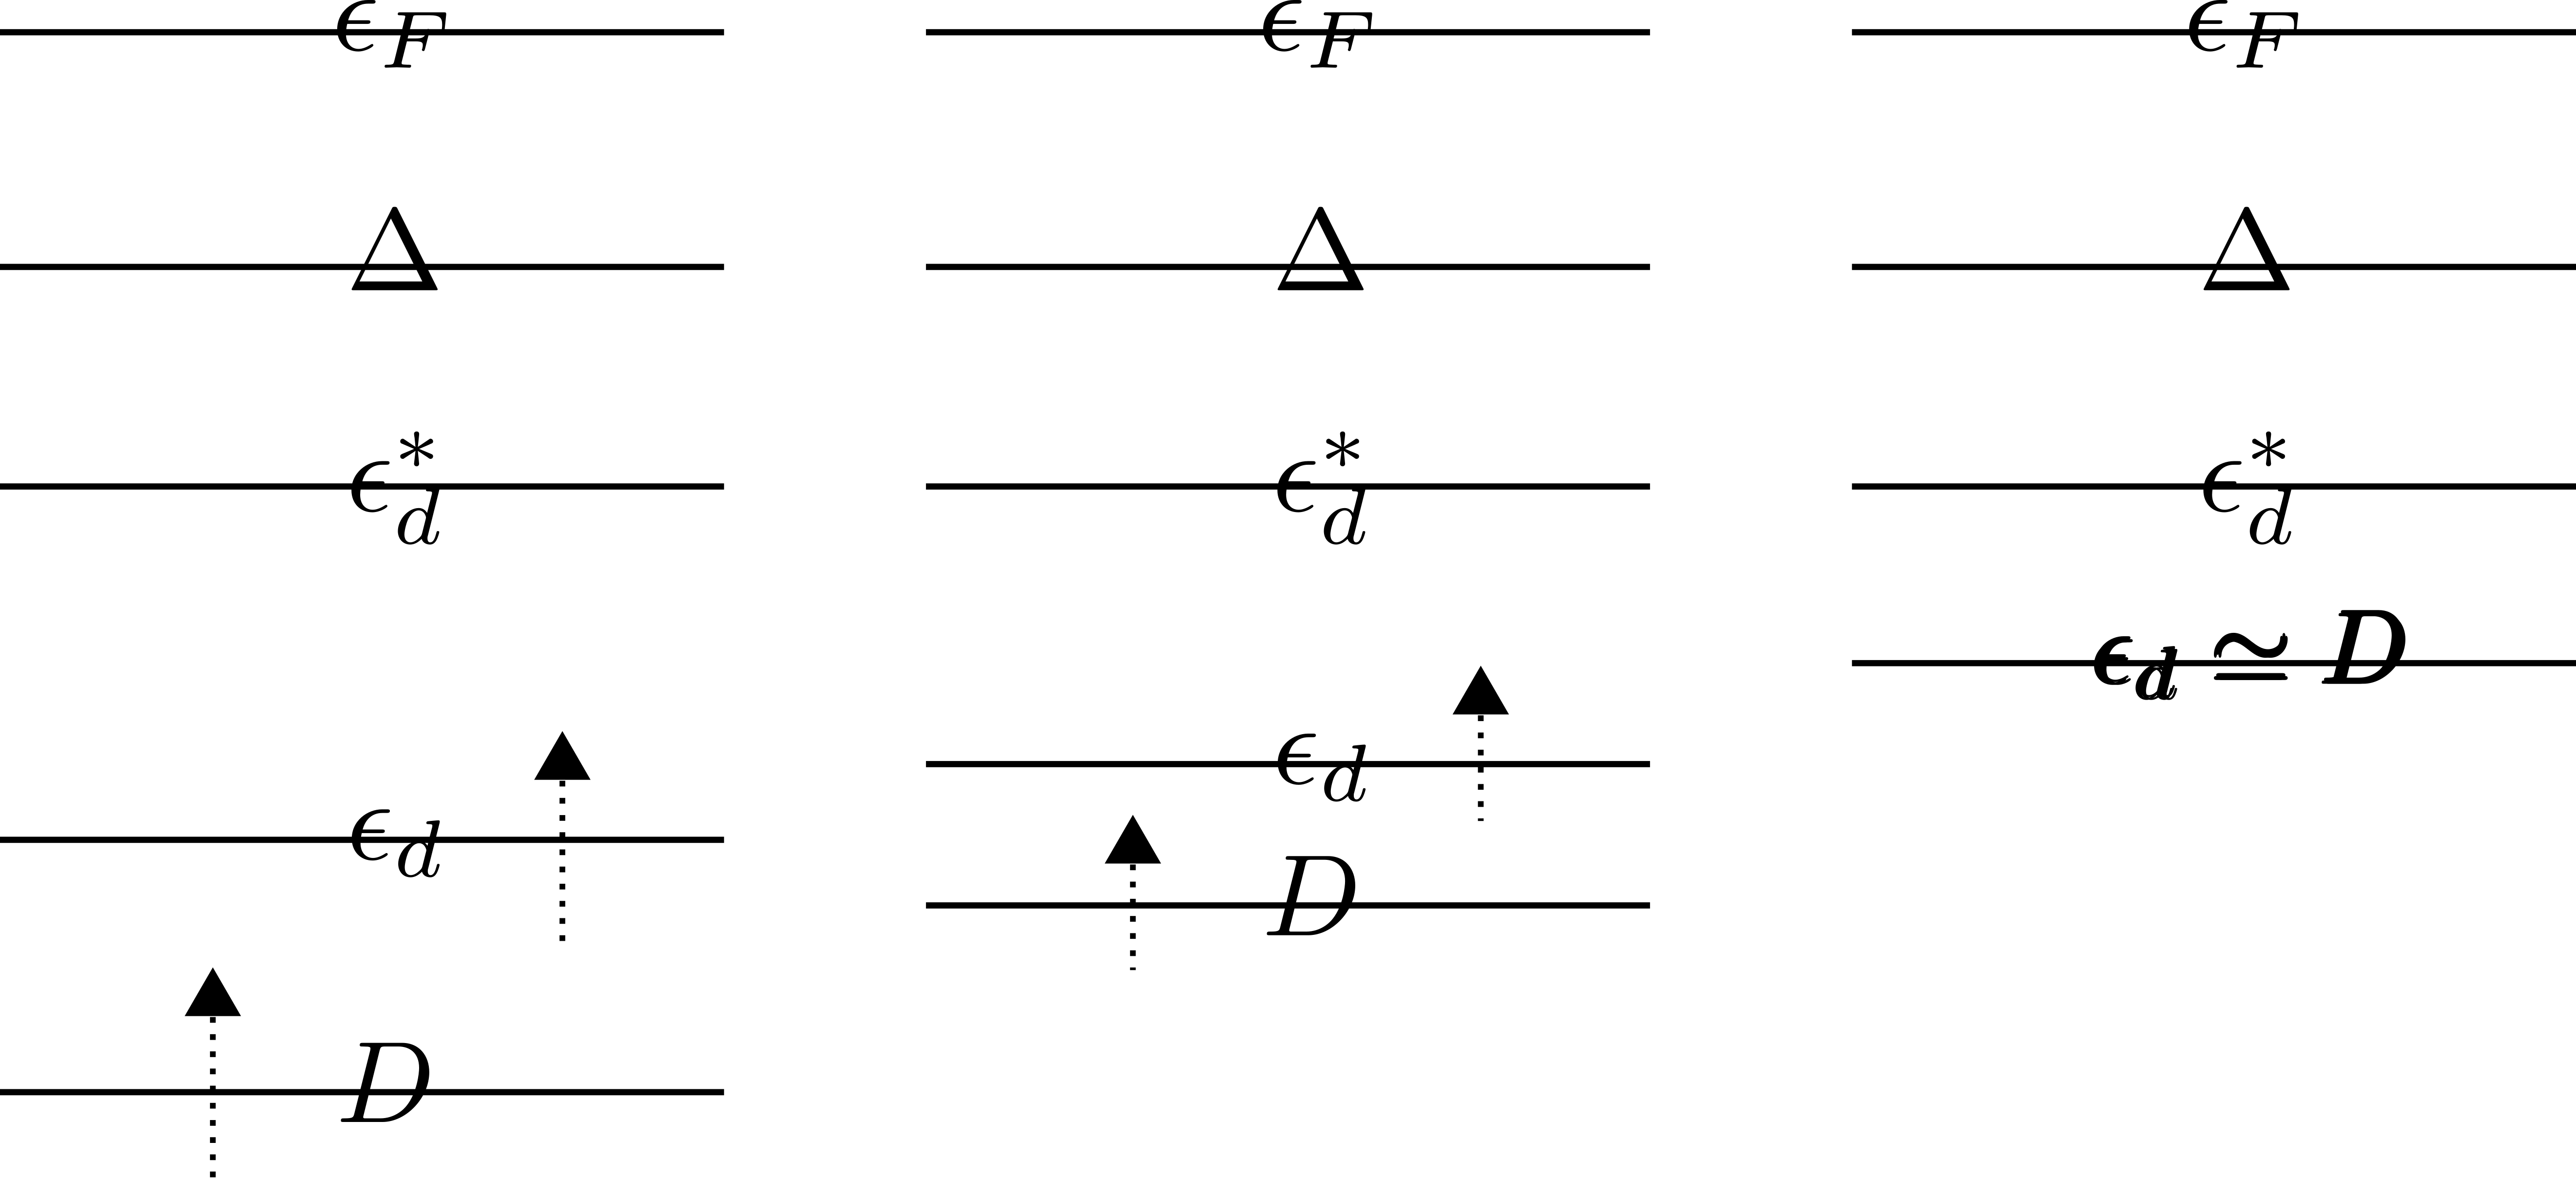
\includegraphics[width=0.6\textwidth]{../figures/empty.png}
	\caption{Renormalization in energy levels when \(\epsilon_d^* \ll -\Delta\)}
\end{figure}

\subsubsection*{Jefferson's calculation}
Jefferson did a slightly more rigorous calculation to obtain the scaling equation.
He divided the Hamiltonian into two parts
\begin{equation}\begin{aligned}
	H = \sum_{k\sigma}\epsilon_{k\sigma} n_{k\sigma} + \epsilon_d n_d + \sum_{k\sigma} \left(V^-_{kd}c^\dagger_{k\sigma}c_{d\sigma} + V^+_{kd}c^\dagger_{d\sigma}c_{k\sigma}\right) = H_0 + V
\end{aligned}\end{equation}
Before scaling, \(V^+ = V^- = V\).
The Schrödinger equation we want to solve is
\begin{equation}\begin{aligned}
H \psi = E \psi
\end{aligned}\end{equation}
We know the eigenstates \(\psi_0\) of \(H_0\).
They are the states \(\{\ket{n_{k_i\sigma},n_{d\sigma^\prime}}\}\).
These states of course span the entire Hilbert space.
A subset of these states form the model subspace.
We call these states \(\phi\).
For our case, that is the subspace with all conduction electrons inside \(D - \delta D\).
The projection operator for this subspace is 
\begin{equation}\begin{aligned}
P = \sum \ket{\phi}\bra{\phi} =  \sum_{|k|<D-\delta D, \sigma=\pm 1, n_{d\sigma}=0,1} \ket{n_{k\sigma},n_{d\sigma^\prime}}
\end{aligned}\end{equation}
Its orthogonal subspace has a projection operator
\begin{equation}\begin{aligned}
Q = 1 - P = \sum_{D-\delta D < |k| < D, \sigma=\pm 1, n_{d\sigma}=0,1} \ket{n_{k\sigma},n_{d\sigma^\prime}}
\end{aligned}\end{equation}
If the dimension of model subspace if \(d\), we can say that \(P\) takes \(d\) eigenstates \(\psi\) of the total Hamiltonian to \(d\) eigenstates in the model subspace:
\begin{equation}\begin{aligned}
P \{\psi\}_d = \{\phi\}
\end{aligned}\end{equation}
This is of course true in the non-interacting limit.
There, the \(\psi_0\) are the exact eigenstates, and the action of \(P\) is basically
\begin{equation}\begin{aligned}
P \psi_0\bigg\vert_{|k|<D-\delta D} = \psi_0\bigg\vert_{|k|<D-\delta D}
\end{aligned}\end{equation}
Now, as we turn on the interactions adiabatically, it is safe to assume that these \(d\) non-interacting eigenstates flow into \(d\) interacting eigenstates.
This means that we can define an inverse for the \(P\) operator which takes a non-interacting eigenstate from the model subspace into the interacting eigenstate:
\begin{equation}\begin{aligned}
\Omega \{\phi\} = \{\psi\}
\end{aligned}\end{equation}
Since \(\Omega\) can only act on states in the model subspace, we define
\begin{equation}\begin{aligned}
\Omega \{\phi\}^\perp = 0
\end{aligned}\end{equation}
This allows us to write
\begin{gather}
\Omega P \phi = \Omega \phi\\
\Omega P \phi^\perp = \Omega \times 0 = 0  = \Omega \phi^\perp
\end{gather}
In the first equation, I used \(P \phi = \phi\) because the projection of \(\phi\) into the model subspace is \(\phi\) itself.
Together these two identities give
\begin{equation}\begin{aligned}
	\label{hikki}
\Omega P = \Omega
\end{aligned}\end{equation}
With these definitions, we now change the problem a bit.
We want to solve the Schrödinger equation only in the model subspace.
To this end we write the Schrödinger equation as
\begin{equation}\begin{aligned}
H \Omega \phi = E \Omega \Phi \\
\end{aligned}\end{equation}
Since we want to write down an equation only in the model subspace, the equation should operate only on the \(\phi\).
To remove the \(\Omega\) on the right side, operate on this equation with \(P\) from the left.
This gives
\begin{equation}\begin{aligned}
P H \Omega \phi = E P \Omega \phi = E \phi\\
\end{aligned}\end{equation}
This is the effective Schrödinger equation in the model subspace.
The effective Hamiltonian for the model subspace is
\begin{equation}\begin{aligned}
	\label{yuigahama}
H_\text{eff} = PH\Omega  = PH_0 P + PV\Omega = P H_0 P + PV\Omega
\end{aligned}\end{equation}
To solve for the \(\Omega\), apply eq.~\ref{hikki} on the Schrödinger equation \((E - H_0)\psi =V \psi\):
\begin{equation}\begin{aligned}
\Omega V\psi = (E \Omega P - \Omega P H_0)\psi
\end{aligned}\end{equation}
Now, since \(P\) is made up of the eigenstates of \(H_0\), those two will commute: \(\left[H_0, P\right] = 0\).
The equation then becomes
\begin{equation}\begin{aligned}
\Omega V\psi = (E - \Omega H_0 P)\psi
\end{aligned}\end{equation}
Subtracting the Schrödinger equation from the last equation gives
\begin{equation}\begin{aligned}
	\left(\Omega - 1\right) V\psi &= \left(H_0 - \Omega H_0 P\right)\psi\\
	\implies \left(\Omega - 1\right) V \Omega \phi &= \left(H_0 - \Omega H_0 P\right)\Omega \phi\\
	\implies \left(\Omega - 1\right) V \Omega \phi &= \left(H_0 \Omega - \Omega H_0\right) \phi\\
	\implies \left(\Omega - 1\right) V \Omega &= \left[H_0, \Omega\right]
\end{aligned}\end{equation}
This is the main equation.
To make progress, we expand the operator \(\Omega\) in powers of the interaction \(V\):
\begin{equation}\begin{aligned}
\Omega = \sum_n c_n V^n = \sum_n \Lambda_n
\end{aligned}\end{equation}
The zeroth term in the main equation becomes
\begin{equation}\begin{aligned}
	\left[H_0, \Lambda_0\right] = 0 \implies \Lambda_0 = P
\end{aligned}\end{equation}
The first order equation is
\begin{equation}\begin{aligned}
	\left[H_0, \Lambda_1\right] = \left(\Lambda_0 - 1\right)V\Lambda_0 = \left(P - 1\right)VP = -QVP
\end{aligned}\end{equation}
The second order equation is
\begin{equation}\begin{aligned}
	\left[H_0, \Lambda_2\right] = -V\Lambda_1 + \Lambda_0 V \Lambda_1 + \Lambda_1 V \Lambda_0 = -QV\Lambda_1 + \Lambda_1 V P
\end{aligned}\end{equation}
These equations are of the form \(\left[H_0, \Lambda_n\right] = A_n\), where \(A_n\) is an operator in terms of \(\Lambda_{n-1}\) and lower orders.
\begin{gather}
A_1 = -QVP\\
A_2 = -QV\Lambda_1 + \Lambda_1 V P
\end{gather}
Let \(\ket{l}\) and \(\ket{h}\) belong to the model subspace and its orthogonal subspace respectively.
Then, taking matrix element between \(\bra{h}\) and \(\ket{l}\) of the general form equation gives
\begin{equation}\begin{aligned}
	\bra{h} A_n \ket{l} = \left(E_h - E_l\right)\bra{h}\Lambda_n \ket{l} \implies \bra{h}\Lambda_n \ket{l} = \frac{\bra{h} A_n \ket{l}}{E_h - E_l}
\end{aligned}\end{equation}
If we define an operator \(S\) by its action on a general operator A as
\begin{equation}\begin{aligned}
\bra{h}S A \ket{l} = \frac{\bra{h} A \ket{l}}{E_l - E_h}
\end{aligned}\end{equation}
we can write the solution
\begin{equation}\begin{aligned}
\Lambda_n = -S(A_n)
\end{aligned}\end{equation}
The expression of \(SA\) can be written as
\begin{equation}\begin{aligned}
SA &= \sum_{h,l}\ket{h}\bra{l} \frac{\bra{h}A\ket{l}}{E_l - E_H} \\
   &= \sum_{h,l}\frac{1}{E_l - E_h}\ket{h}\bra{h}A\ket{l}\bra{l}\\
   &= \sum_{l}\frac{1}{E_l - H_0}\left(\sum_h \ket{h}\bra{h}\right)A\ket{l}\bra{l}\\
   &= \sum_l G_l A P_l
\end{aligned}\end{equation}
where \(P_l = \ket{l}\bra{l}\) and \(G_l = \frac{1}{E_l - H_0}Q\).\\\\
\(S\) has the property
\begin{equation}\begin{aligned}
\bra{h}S QA \ket{l} &= \frac{\bra{h}Q A \ket{l}}{E_l - E_h} = \frac{\bra{h}A \ket{l}}{E_l - E_h} = \bra{h}SA\ket{l} \\
\implies S(QA) &= S(A)
\end{aligned}\end{equation}
The lowest order solutions are thus
\begin{gather}
    \Lambda_1 = S(QVP) = S(VP)\\
    \Lambda_2 = S(QV\Lambda_1) - S(\Lambda_1 V P) = S(VS(VP)) - S(S(VP)VP)
\end{gather}
We can now expand the effective Hamiltonian in powers of \(V\).
From eq.~\ref{yuigahama}, the interacting part of the effective Hamiltonian becomes
\begin{equation}\begin{aligned}
H_\text{eff} - P H_0 P &= P V\Omega \\
               &\approx PV(\Lambda_0 + \Lambda_1 + \Lambda_2)\\
	       &= PV\left[P + S(VP) + S(VS(VP)) - S(S(VP)VP)\right]\\
                   &= PVP + PVS(VP) + PVS(VS(VP)) - PVS(S(VP)VP)
\end{aligned}\end{equation}
Therefore,
\begin{equation}\begin{aligned}
H_\text{eff} = PHP + PVS(VP) + PVS(VS(VP)) - PVS(S(VP)VP)
\end{aligned}\end{equation}
The first term is the obvious lowest approximation; you just project the entire Hamiltonian into the model subspace.
 The second term is
 \begin{equation}\begin{aligned}
PVSVP = PV \sum_l G_l V P P_l = PV \sum_l G_l V P_l
\end{aligned}\end{equation}
where I used \(P P_l = \sum_{l^\prime} \ket{l^\prime}\bra{l^\prime} \ket{l}\bra{l} = \sum_{l^\prime}\ket{l^\prime}\bra{l^\prime}\delta_{ll^\prime} = P_l\).
The third term becomes
\begin{equation}\begin{aligned}
PVSVSVP  = PVSV \sum_l G_l V P_l = PV\sum_l S V G_l V P_l \\
= PV\sum_{l,l^\prime} G_{l^\prime} V G_l V P_lP_{l^\prime} = PV \sum_l  G_{l} V G_l V P_l
\end{aligned}\end{equation}
The fourth term is
\begin{equation}\begin{aligned}
PVS(S(VP)VP) = PVS(\sum_l G_l VP P_l VP) = PV \sum_{l,l^\prime} G_{l^\prime} G_l VP_l VP P_{l^\prime} \\
= PV \sum_{l^\prime} G_{l^\prime} \left(\sum_l G_l VP_l\right) V P_{l^\prime}
\end{aligned}\end{equation}
The effective Hamiltonian up to third order in \(V\) is
\begin{equation}\begin{aligned}
H_\text{eff} = PH_0 P + PV \sum_l G_l V P_l + PV \sum_l  G_{l} V G_l V P_l \\
- PV \sum_{l,l^\prime} G_{l^\prime} G_l VP_l V P_{l^\prime}
\end{aligned}\end{equation}
These results have been more or less general.
We now need to write these in terms of the creation and annihilation operators of our Hamiltonian.
The model subspace for our problem is the part of the conduction band up to \(D - \delta D\).
Here on, \(\sum\) represent sum over the model subspace momenta and \(\sum^\prime\) represent sum over the remaining momenta.
To facilitate writing the effective Hamiltonian in terms of the creation and annihilation operators, we change the projection operators from the bra-ket representation to operator representation:
\begin{gather}
    \ket{k_1}\bra{k_2} = c^\dagger_{k_1}c_{k_2} \\
    P_k = \ket{k,n_{d\sigma}}\bra{k,n_{d\sigma}} = c^\dagger_{k}c_{k}c^\dagger_{d\sigma}c_{d\sigma} = n_{k\sigma}n_{d\sigma}
\end{gather}
The first term becomes
\begin{equation}\begin{aligned}
	P H_0 P = \sum_{k\sigma} \epsilon_{k\sigma} n_{k\sigma} + \epsilon_d n_d + \sum_{k\sigma}\left(V_{kd} c^\dagger_{k\sigma} c_{d\sigma} + \text{h.c.}\right)
\end{aligned}\end{equation}
The second term involves two potential terms that scatter from the model subspace to the high energy subspace and then back to the model subspace.
Hence this term is 
\begin{equation}\begin{aligned}
	PV \sum_l G_l V P_l  &= V \sum_{q\sigma}\left(\frac{V_q}{\epsilon_d - \epsilon_q} c^\dagger_{q\sigma}c_{d\sigma} + \frac{V^*_q}{\epsilon_q - \epsilon_d} c^\dagger_{d\sigma}c_{q\sigma}\right)\\
             &= {\sum_{q\sigma}}^+\frac{|V_q|^2 c^\dagger_{d\sigma}c_{q\sigma} c^\dagger_{q\sigma}c_{d\sigma}}{\epsilon_d - \epsilon_q} + {\sum_{q\sigma}}^-\frac{|V_q|^2c^\dagger_{q\sigma}c_{d\sigma}c^\dagger_{d\sigma}c_{q\sigma}}{\epsilon_q - \epsilon_d}\\
	     &= {\sum_{q\sigma}}^+\frac{|V_q|^2 n_{d\sigma}\left(1-n_{q\sigma}\right)}{\epsilon_d - \epsilon_q} + {\sum_{q\sigma}}^-\frac{|V_q|^2n_{q\sigma}\left(1-n_{d\sigma}\right)}{\epsilon_q - \epsilon_d}\\
\end{aligned}\end{equation}
In the high energy subspaces, \(n_q^+ = 1-n_q^- = 0\).
Therefore,
\begin{equation}\begin{aligned}
	PV \sum_l G_l V P_l  &= {\sum_q}^+\frac{|V_q|^2 n_{d\sigma}}{\epsilon_d - \epsilon_q} + {\sum_q}^-\frac{|V_q|^2\left(1-n_{d\sigma}\right)}{\epsilon_q - \epsilon_d} \\
			     &= n_d \left({\sum_q}^+\frac{|V_q|^2 }{\epsilon_d - \epsilon_q} + 2{\sum_q}^-\frac{|V_q|^2}{\epsilon_d - \epsilon_q}\right)\\
             &= n_d \delta \epsilon_d
\end{aligned}\end{equation}
The third term is zero in our case.
The part \(G_l V G_l V\) will do the following.

\begin{equation}\begin{aligned}
\ket{k,n_{d\sigma}} \rightarrow \begin{cases} \ket{q_e,n_d=0} \rightarrow \begin{cases} \ket{q_e,n_d=1}\\\ket{q_e,q^\prime_h,n_d = 1} \end{cases}
\\ 
\ket{q_h,n_d=1} \rightarrow \begin{cases} \ket{q_h,q^\prime_e,n_d=0} \\ \ket{q_h,n_d=0} \end{cases}
\end{cases} 
\end{aligned}\end{equation}
None of the four final states belong to the model subspace, so this term is zero.\\\\
The fourth term involves a first scattering between two model states, followed by a scattering to a high energy subspace and then a scattering back to the model subspace.
One way for going through such a process is
\begin{equation}\begin{aligned}
\ket{k,n_d = 0} \underbrace{\rightarrow \ket{n_d=1} \rightarrow}_{\Delta E = \epsilon_k - \epsilon_q} \ket{q_e,n_d = 0} \underbrace{\rightarrow}_{\Delta E = \epsilon_q - \epsilon_d} \ket{k^\prime, n_d = 1}
\end{aligned}\end{equation}
Another way is to start with \(c_d\) instead of \(c^\dagger_d\) 
\begin{equation}\begin{aligned}
\ket{n_{d\sigma} = 1} \underbrace{\rightarrow \ket{k\sigma,n_d=0} \rightarrow}_{\Delta E = \epsilon_k - \epsilon_q} \begin{cases} \ket{q_h\uparrow, n_{d\uparrow} = 1}\\ \ket{q_h\downarrow, n_{d\downarrow} = 1} \end{cases} \underbrace{\rightarrow}_{\Delta E = \epsilon_q - \epsilon_d} \ket{n_d = 0}
\end{aligned}\end{equation}
Combining the two processes gives

\begin{equation}\begin{aligned}
{\sum_{q}}^+\sum_{k\sigma} \frac{|V_q|^2c^\dagger_{d\sigma}c_{q\sigma}c^\dagger_{q\sigma}c_{d\sigma}c^\dagger_{d\sigma}c_{k\sigma}}{(\epsilon_q - \epsilon_d)(\epsilon_k - \epsilon_q)} + {\sum_{q\sigma^\prime}}^-\sum_{k\sigma} \frac{|V_q|^2c^\dagger_{q\sigma^\prime}c_{d\sigma^\prime}c^\dagger_{d\sigma^\prime}c_{q\sigma^\prime}c^\dagger_{k\sigma}c_{d\sigma}}{(\epsilon_q - \epsilon_d)(\epsilon_k - \epsilon_q)}\\
=\sum_{k\sigma}\left(c^\dagger_{k\sigma}c_{d\sigma} \delta V^-_k + c^\dagger_{d\sigma}c_{k\sigma}\delta V^-_k\right)
\end{aligned}\end{equation}
where
\begin{equation}\begin{aligned}
\delta V^+ = {\sum_q}^+ \frac{|V_q|^2}{(\epsilon_q - \epsilon_d)(\epsilon_k - \epsilon_q)}\\
\delta V^- = {\sum_q}^- 2\frac{|V_q|^2}{(\epsilon_q - \epsilon_d)(\epsilon_k - \epsilon_q)}
\end{aligned}\end{equation}
The total Hamiltonian can be written in the form
\begin{equation}\begin{aligned}
	H_\text{eff} = \sum_{k\sigma}\epsilon_{k\sigma} n_{k\sigma} + &\left(\epsilon_d + \delta \epsilon_d\right)n_d \\
	+ &\sum_{k\sigma}\left\{\left(V^-_k + \delta V^-_k\right) c^\dagger_{k\sigma}c_{d\sigma} + \left(V^+_k + \delta V^+_k\right) c^\dagger_{d\sigma}c_{k\sigma}\right\}
					     \end{aligned}\end{equation}
We now evaluate the changes:
\begin{equation}\begin{aligned}
	\delta \epsilon_d &= \left({\sum_q}^+\frac{|V_q|^2 }{\epsilon_d - \epsilon_q} + 2{\sum_q}^-\frac{|V_q|^2}{\epsilon_d - \epsilon_q}\right) \\
			  &\approx |V|^2 \rho |\delta D| \left(\frac{1}{\epsilon_d - D} + \frac{2}{\epsilon_d + D}\right)\\
&=|V|^2 \rho |\delta D|\frac{D - 3\epsilon_d}{D^2 - \epsilon_d^2}
\end{aligned}\end{equation}
I used the approximation
\begin{equation}\begin{aligned}
\sum_{q=D-\delta D}^D f(q) = \int_{D- \delta D}^D dE \rho(E) f(E) \approx \rho f(D) \delta D
\end{aligned}\end{equation}
Also,
\begin{equation}\begin{aligned}
\delta V_k^+ &= {\sum_q}^+ \frac{|V_q|^2}{(\epsilon_q - \epsilon_d)(\epsilon_k - \epsilon_q)}\\
           &\approx |V|^2 \rho |\delta D|\frac{1}{(D - \epsilon_d)(\epsilon_k - D)}\\
\delta V_k^- &= 2{\sum_q}^- \frac{|V_q|^2}{(\epsilon_q - \epsilon_d)(\epsilon_k - \epsilon_q)}\\
           &\approx -|V|^2 \rho |\delta D|\frac{2}{(D + \epsilon_d)(\epsilon_k + D)}
\end{aligned}\end{equation}
We now make the following assumptions:
\begin{itemize}
	\item \(k\) is close to the Fermi level (\(\epsilon_k \approx 0\))
	\item Because \(k\) is close to the Fermi surface, we assume the potential is independent of momenta: \(V_k^+ \equiv v^+, V^-_k \equiv v^-\)
	\item Since we truncated at third order, we need \(D - |\epsilon_d| \gg v^\pm\).
		This gives us \(D \gg |\epsilon_d|\).
\end{itemize}
With these assumptions, we get the scaling equations similar to the ones obtained previously.
%\)
\section{Numerical Renormalization Group Calculation of the symmetric SIAM}
NRG calculations of the symmetric SIAM were carried out by H. R. Krishnamurthy, Wilkins and Wilson in ref.~\cite{hrk-nrg}. They identified three fixed points in the phase diagram. Two of them, the free-orbital and the local moment, are unstable while the strong-coupling fixed point is stable. These fixed points along with typical RG flows are marked in fig.~\ref{nrg_fp}.
\begin{figure}[htpb]
	\centering
	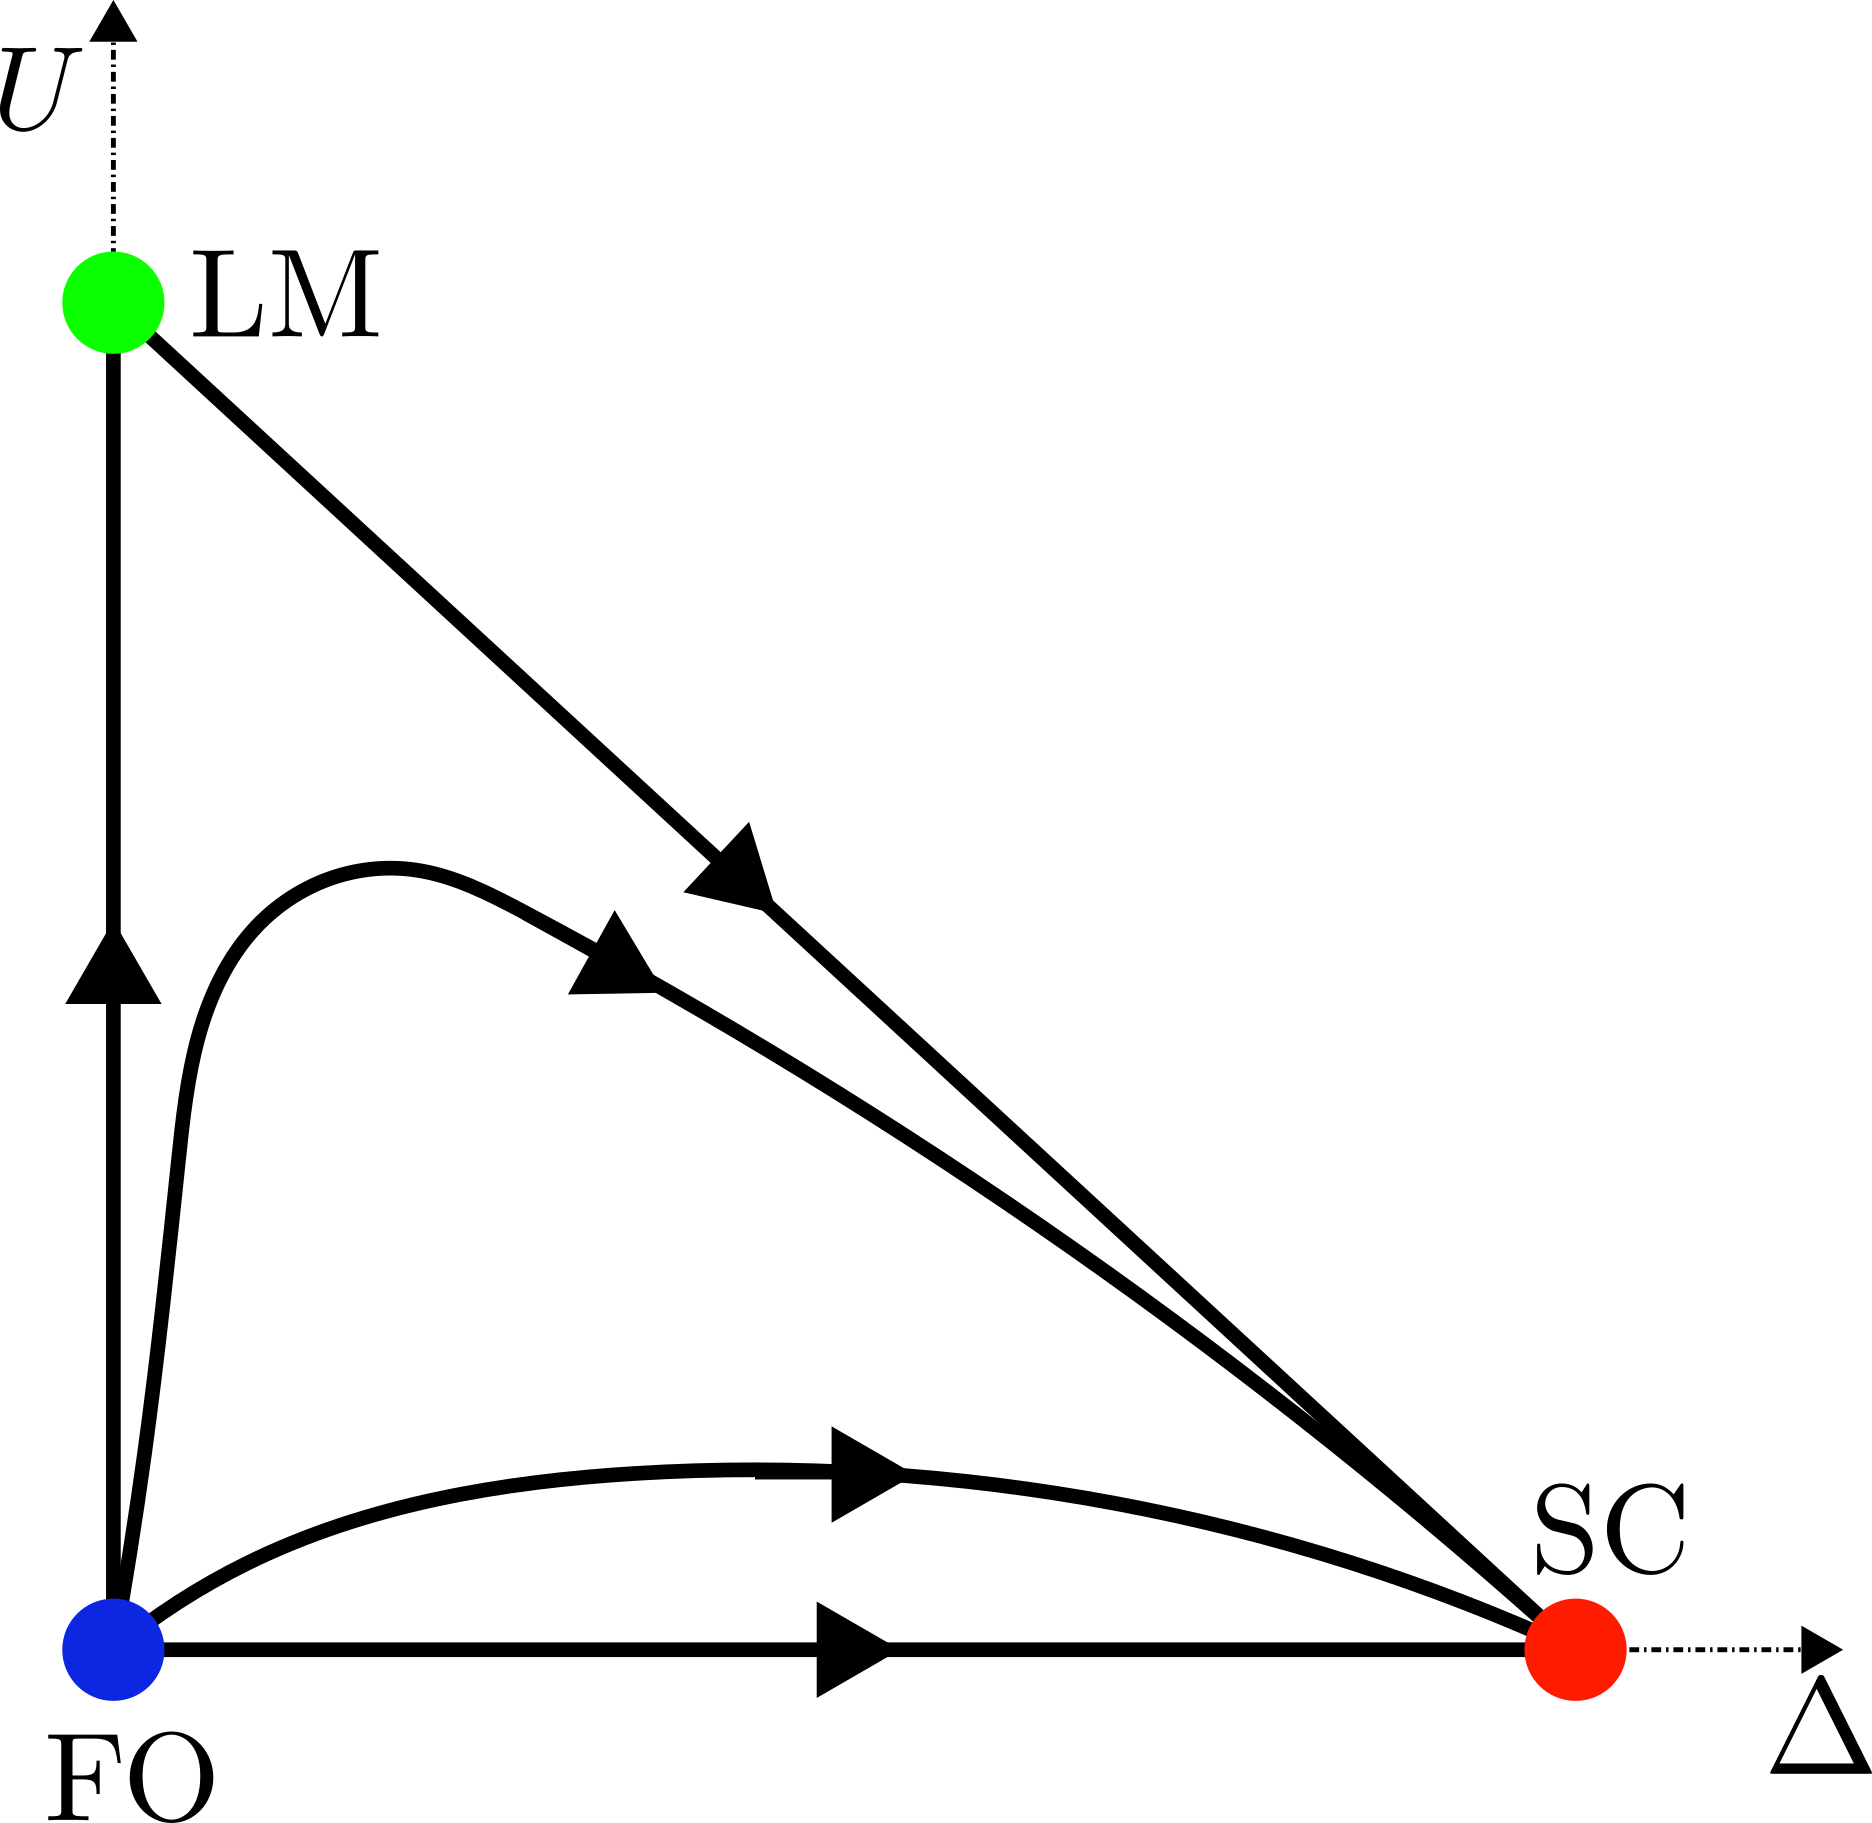
\includegraphics[width=0.5\textwidth]{../figures/nrg_fpoints.png}
	\caption{Schematic diagram of RG flows and fixed points of the symmetric SIAM, as obtained by ref.\cite{hrk-nrg}. The y-axis is the impurity site repulsion \(U = -\frac{1}{2}\epsilon_d\) while the x-axis is the hybridisation parameter \(\Delta \sim \rho V^2\). The abbreviations mark the three fixed-points: FO is free-orbital, LM is local moment and SC is strong-coupling. The fixed-points are described in the text.}
	\label{nrg_fp}
\end{figure}
The free-orbital fixed point is described by \(U=V=0\). The local moment fixed point is described by \(U \to \infty, V=0\). The strong-coupling fixed point is described by \(U=\text{finite}, V \to \infty\). The temperature-dependent susceptibility is found to be very similar to that obtained from the Kondo model, with a suitably-defined \(T_K\). It starts from a constant value at low-temperatures to a Curie-Weiss like form at high temperatures, with the Curie-Weiss constant at very large temperatures being equal to \(\frac{1}{8}\).

\chapter{Unitary Renormalization Group Method}\label{urgform}
The URG method was introduced and formalised in refs.~\cite{anirbanurg1,anirbanurg2,anirbanmott1,anirbanmott2}.  This section is adapted from those references and expanded wherever required.
\section{Formalism and Results}
\subsection{Description of the problem}
We are given a Hamiltonian \(\mathcal{H}\) which is not completely diagonal in the occupation number basis of the electrons, \(\hat n_k\): \(\left[\mathcal{H},n_k\right] \neq 0\). \(k\) labels any set of quantum numbers depending on the system. For spin-less Fermions it can be the momentum of the particle, while for spin-full Fermions it can be the set of momentum and spin. There are terms that scatter electrons from one quantum number \(k\) to another quantum number \(k^\prime\).
\\\\We take a general Hamiltonian,
\begin{equation}\begin{aligned}
	\mathcal{H} = H_e \hat n_{q\beta} + H_h \left(1 - \hat n_{q\beta}\right) + c^\dagger_{q\beta}T + T^\dagger c_{q\beta}
\end{aligned}\end{equation}
Formally, we can decompose the entire Hamiltonian in the subspace of the electron we want to decouple (\(q\beta\)).
\begin{equation}\begin{aligned}
	\label{matham}
\mathcal{H} = \bordermatrix{~ & \ket{1} & \ket{0} \cr
              & H_1 & T \cr
              & T^\dagger & H_0 \cr}
\end{aligned}\end{equation}
The basis in which this matrix is written is \(\left\{\ket{1},\ket{0}\right\}\) where \(\ket{i}\) is the set of all states where \(\hat n_{q\beta}=i\). The aim of one step of the URG is to find a unitary transformation \(U\) such that the new Hamiltonian \(U \mathcal{H} U^\dagger\) is diagonal in this already-chosen basis.
\begin{equation}\begin{aligned}
	\tilde{\mathcal{H}} \equiv U \mathcal{H} U^\dagger = \bordermatrix{~ & \ket{1} & \ket{0} \cr
              & \tilde H_1 & 0 \cr
              & 0 & \tilde H_0 \cr}
\end{aligned}\end{equation}
\(U_q\) is defined by
\begin{equation}\begin{aligned}
	\tilde{\mathcal{H}} = U_q \mathcal{H} U^\dagger_q \text{   such that  } \left[\tilde{\mathcal{H}},n_q\right] = 0
\end{aligned}\end{equation}
It is clear that \(U\) is the diagonalizing matrix for \(\mathcal{H}\). Hence we can frame this problem as an eigenvalue equation as well. Let \(\ket{\psi_1},\ket{\psi_0}\) be the basis in which the original Hamiltonian \(\mathcal{H}\) has no off-diagonal terms corresponding to \(q\beta\). Hence, we can write
\begin{equation}\begin{aligned}
	\label{diageq}
    \mathcal{H} \ket{\psi_i} = \tilde H_i\ket{\psi_i}, i\in\left\{0,1\right\}
\end{aligned}\end{equation}
Since \(\ket{\psi_i}\) is the set of eigenstates of \(\mathcal{H}\) and \(\ket{i}\) is the set of eigenstates in which \(U\mathcal{H} U^\dagger\) has no off-diagonal terms corresponding to \(q\beta\), we can relate \(\ket{\psi_i}\) and \(\ket{i}\) by the same transformation : \(\ket{\psi_i} = U^\dagger\ket{i}\). We can expand the state \(\ket{\psi_i}\) in the subspace of \(q\beta\):
\begin{equation}\begin{aligned}
	\label{matpsi}
\ket{\psi_i} = \sum_{j=0,1} \ket{j}\bra{j}\ket{\psi_i} \equiv \ket{1}\ket{\phi_1^i} + \ket{0}\ket{\phi_0^i}\end{aligned}\end{equation}
where \(\ket{\phi_j^i} = \bra{j}\ket{\psi_i}\). If we substitute the expansion \ref{matham} into the eigenvalue equation \ref{diageq}, we get
\begin{equation}\begin{aligned}
	\left[H_e \hat n_{q\beta} + H_h \left(1 - \hat n_{q\beta}\right) + c^\dagger_{q\beta}T + T^\dagger c_{q\beta}\right]\ket{\psi_i} = \tilde H_i\ket{\psi_i}
\end{aligned}\end{equation}
The diagonal parts \(H_e = \text{tr}\left[\mathcal{H} \hat n_{q\beta}\right]\) and \(H_e = \text{tr}\left[\mathcal{H} \left(1 - \hat n_{q\beta}\right)\right]\) can be separated into a purely diagonal part \(\mathcal{H}^d\) that contains the single-particle energies and the multi-particle correlation energies or Hartree-like contributions, and an off-diagonal part  \(\mathcal{H}^i\) that scatters between the remaining degrees of freedom \(k\sigma \neq q\beta\). That is,
\begin{equation*}
\begin{gathered}
	H_e \hat n_{q\beta} + H_h \left(1 - \hat n_{q\beta}\right) = \mathcal{H}^d + \mathcal{H}^i\\
\end{gathered}
\end{equation*}
This gives
\begin{equation}\begin{aligned}
	\left[c^\dagger_{q\beta}T + T^\dagger c_{q\beta}\right]\ket{\psi_i} = \left(\tilde H_i - \mathcal{H}^i - \mathcal{H}^d\right)\ket{\psi_i}
\end{aligned}\end{equation}
\subsection{Obtaining the decoupling transformation}
We now define a new operator \(\hat \omega_i = \tilde H_i - \mathcal{H}^i\), such that 
\begin{equation}\begin{aligned}
	\left[c^\dagger_{q\beta}T + T^\dagger c_{q\beta}\right]\ket{\psi_i} = \left(\hat \omega_i - \mathcal{H}^d\right)\ket{\psi_i}
\end{aligned}\end{equation}
From the definition of \(\hat \omega_i\), we can see that it is Hermitian and has no term that scatters in the subspace of \(q\beta\), so it is diagonal in \(q\beta\) and we can expand it as \(\hat \omega_i = \hat \omega_i^1 \hat n_{q\beta} + \hat \omega_i^0 \left(1 - \hat n_{q\beta}\right)\). Using the expansion \ref{matpsi}, we can write
\begin{equation}\begin{aligned}
\hat \omega_i \ket{\psi_i} = \hat \omega_i^1 \ket{1}\ket{\phi_1^i} + \hat \omega_i^0 \ket{0}\ket{\phi_0^i}
\end{aligned}\end{equation}
Since the only requirement on \(\ket{\psi_i}\) is that it diagonalize the Hamiltonian in the subspace of \(q\beta\), there is freedom in the choice of this state. We can exploit this freedom and choose the \(\ket{\phi_{0,}^i}\) to be an eigenstates of \(\hat \omega_i^{1,0}\) corresponding to real eigenvalues \(\omega_i^{1,0}\):
\begin{equation}\begin{aligned}
	\left[\mathcal{H}^d + c^\dagger_{q\beta}T + T^\dagger c_{q\beta}\right]\ket{\psi_i(\omega_i)} = \left(\omega_i^1 - \mathcal{H}^d\right)\ket{1}\ket{\phi_1^i} + \left(\omega_i^0 - \mathcal{H}^d\right)\ket{0}\ket{\phi_0^i}
\end{aligned}\end{equation}
If we now substitue the expansion \ref{matpsi} and gather the terms that result in \(\hat n_{q\beta}=1\), we get
\begin{equation}\begin{aligned}
	\label{changea}
	c^\dagger_{q\beta}T\ket{0}\ket{\phi_0^i} = \left(\omega_i^1 - \mathcal{H}^d\right)\ket{1}\ket{\phi_1^i}
\end{aligned}\end{equation}
Similarly, gathering the terms that result in \(\hat n_{q\beta}=0\) gives
\begin{equation}\begin{aligned}
	\label{changeb}
	T^\dagger c_{q\beta}\ket{1}\ket{\phi_1^i} = \left(\omega_i^0 - \mathcal{H}^d\right)\ket{0}\ket{\phi_0^i}
\end{aligned}\end{equation}
We now define two many-particle transition operators:
\begin{equation}\begin{aligned}
	\label{etadefine}
{\eta}^\dagger(\omega_i^1) = \frac{1}{\omega_i^1- \mathcal{H}^d}c^\dagger_{q\beta}T \equiv G_1 c^\dagger_{q\beta}T\\
\eta(\omega_i^0) = \frac{1}{\omega_i^0- \mathcal{H}^d}T^\dagger c_{q\beta} \equiv G_0 T^\dagger c_{q\beta}
\end{aligned}\end{equation}
wher \(G_j\) is the propagator \(\frac{1}{\omega_i^j- \mathcal{H}^d}\). We can write this compactly as
\begin{equation}\begin{aligned}
	\label{etadagdef}
\eta(\hat \omega) = GT^\dagger c_{q\beta} = \frac{1}{\hat \omega_i- \mathcal{H}^d}T^\dagger c_{q\beta}
\end{aligned}\end{equation}
where \(\hat \omega_i = \omega_i^0\left(1 - \hat n_{q\beta}\right) + \omega_i^1\hat n_{q\beta} = \begin{pmatrix} \omega_i^1 & \\ & \omega_i^0 \end{pmatrix}\) is a 2x2 matrix and \(\mathcal{H}^d = \mathcal{H}^d_0\left(1 - \hat n_{q\beta}\right) + \mathcal{H}^d_1\hat n_{q\beta}\) and \(G = \left(\hat \omega - \mathcal{H}^d\right)^{-1}\). It is easy to check that this reproduces the previous forms of \(\eta_0\) and \(\eta_1^\dagger\).
We will later find that it is important to demand that these two be Hermitian conjugates of each other; that constraint is imposed on the denominators:
\begin{equation}\begin{aligned}
	\label{constraint}
\eta^\dagger(\omega_i^0) = \eta^\dagger(\omega_i^1) \implies \frac{1}{\omega_i^1- \mathcal{H}^d}c^\dagger_{q\beta}T = c^\dagger_{q\beta}T\frac{1}{\omega_i^0- \mathcal{H}^d}
\end{aligned}\end{equation}
Henceforth we will assume that this constraint has been imposed. 
\\\\In terms of these operators, eq.~\ref{changeb} becomes
\begin{equation}\begin{aligned}
    \ket{1}\ket{\phi_1^i} &= {\eta}^\dagger\ket{0}\ket{\phi_0^i}\\
    \ket{0}\ket{\phi_0^i} &= \eta\ket{1}\ket{\phi_1^i}
\end{aligned}\end{equation}
These allow us to write
\begin{equation}\begin{aligned}
	\label{trans}
	\ket{\psi_1} &= \ket{1}\ket{\phi_1^i} + \ket{0}\ket{\phi_0^i} = \left(1 + \eta\right)\ket{1}\ket{\phi_1^i}\\
	\ket{\psi_0} &= \left(1 + {\eta}^\dagger\right)\ket{0}\ket{\phi_0^i}
\end{aligned}\end{equation}
Recalling that \(\ket{\psi_i} = U^\dagger \ket{i}\), we can read off the required transformation:
\begin{equation}\begin{aligned}
	\label{Ui}
    U_1 &= 1 + \eta
\end{aligned}\end{equation}

\begin{figure}[htpb]
\begin{center}
	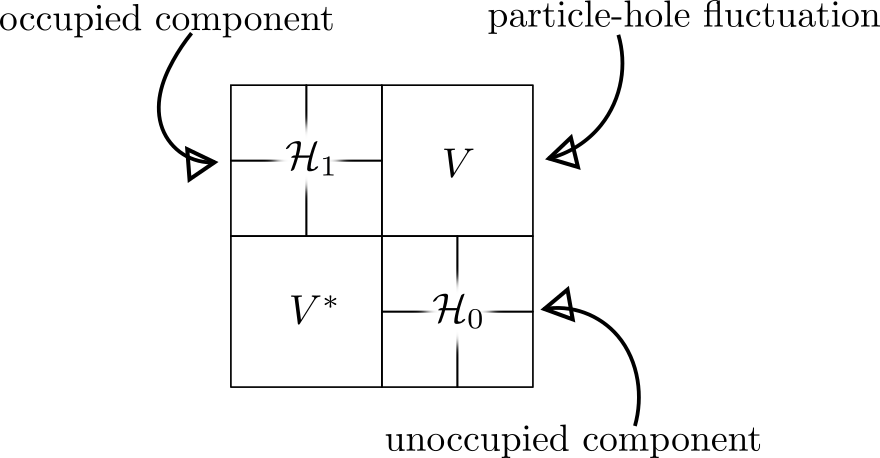
\includegraphics[width=0.7\textwidth]{../figures/matrix.png}
\end{center}
\begin{center}
\def\svgwidth{0.8\columnwidth}
\input{../figures/rotation.pdf_tex}
\end{center}
\begin{center}
	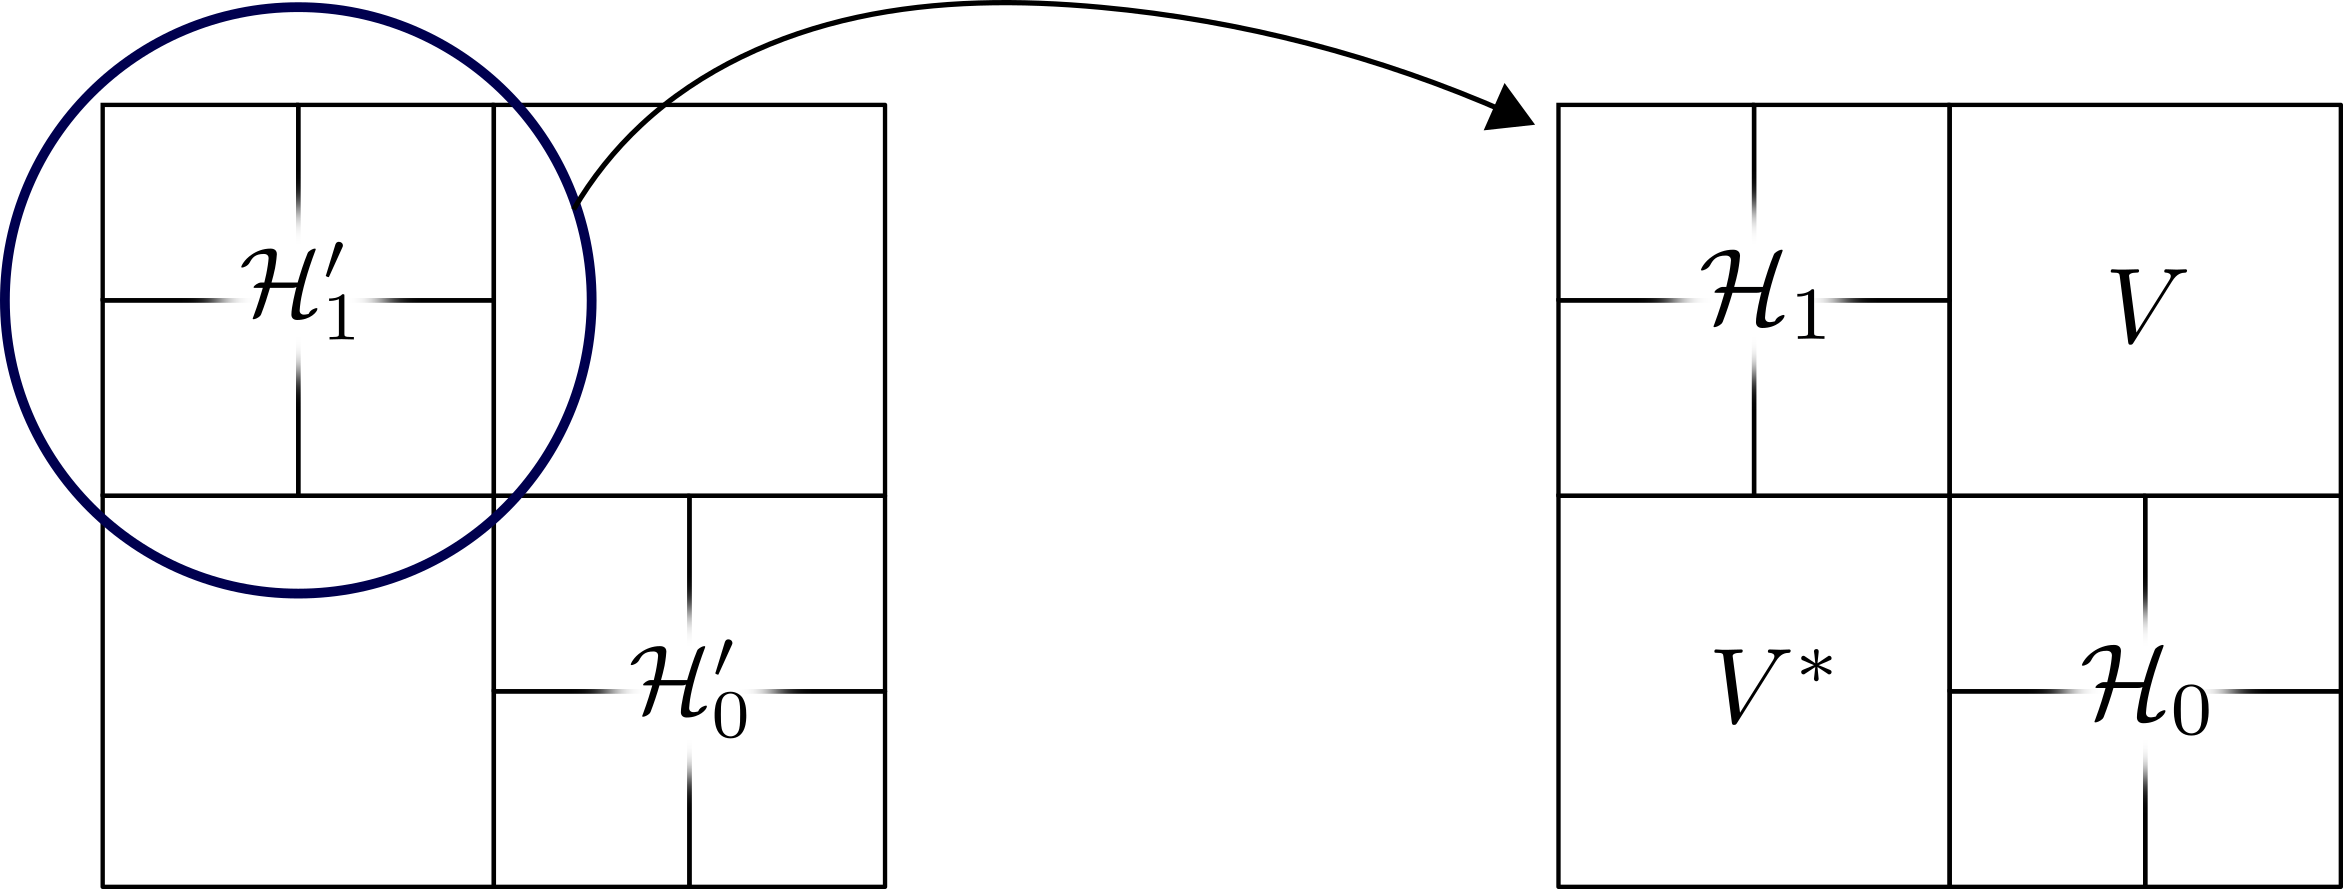
\includegraphics[width=0.8\textwidth]{../figures/repeat.png}
\end{center}
\caption{Three steps of the URG: Decompose the Hamiltonian in a \(2\times 2\) matrix, apply the unitary operator to rotate it, then repeat these steps with one of the rotated blocks.}
\end{figure}
% \begin{figure}
% \def\svgwidth{0.8\columnwidth}
% \centering
% \input{../figures/repeat.pdf_tex}
% \end{figure}

\subsection{Properties of the many-body transition operators}
The operators \(\eta\) have some important properties. First is the Fermionic nature:
\begin{equation}\begin{aligned}
	\eta^2 = {\eta^\dagger}^2 = 0 &&\left[{c^\dagger}^2 = c^2 = 0\right]\\
\end{aligned}\end{equation}
Second is:
\begin{equation}\begin{aligned}
	\label{antic}
    \ket{1}\ket{\phi_1^i} &= {\eta}^\dagger\ket{0}\ket{\phi_0^i} = \eta^\dagger \eta \ket{1}\ket{\phi_1^i} \implies \eta^\dagger \eta = \hat n_{q\beta}\\
    \ket{0}\ket{\phi_0^i} &= \eta\ket{1}\ket{\phi_1^i} = \eta \eta^\dagger\ket{\phi_0^i}\implies \eta  \eta^\dagger= 1 - \hat n_{q\beta}
\end{aligned}\end{equation}
and hence the anticommutator
\begin{equation}\begin{aligned}
	\label{antico}
    \implies \left\{\eta,\eta^\dagger\right\} = 1
\end{aligned}\end{equation}
Note that the three equations in \ref{antic} work only when applied on the eigenstate \(\ket{\psi_i}\) and not any arbitrary state.
\begin{equation*}
    \begin{gathered}
    \eta^\dagger \eta \ket{\psi_i} = \ket{1}\ket{\phi_1^i} = \hat n_{q\beta}\ket{\psi_i}\\
    \eta\eta^\dagger \ket{\psi_i} = \ket{0}\ket{\phi_0^i} = \left(1 - \hat n_{q\beta}\right)\ket{\psi_i}\\
    \left\{\eta^\dagger,\eta\right\}\ket{\psi_i} = \ket{\psi_i}
\end{gathered}
\end{equation*}
\subsection{Form of the unitary operators}\label{unitary-form}
Although we have found the correct similarity transformations \(U_i\) (eqs. \ref{Ui}), we need to convert them into a unitary transformation. Say we are trying to rotate the eigenstate \(\ket{\psi_1}\) into the state \(\ket{1}\). We can then work with the transformation
\begin{equation}\begin{aligned}
U_1 = 1 + \eta
\end{aligned}\end{equation}
In this form, this transformation is not unitary. It can however be written in an exponential form:
\begin{equation}\begin{aligned}
U_1 = e^{\eta}
\end{aligned}\end{equation}
using the fact that \(\eta^2 = 0\). It is shown in ref.~\cite{suzuki} that corresponding to a similarity transformation \(e^\omega\),there exists a unitary transformation \(e^G\) where
\begin{equation}\begin{aligned}
	G = \tanh^{-1}\left(\omega - \omega^\dagger\right)
\end{aligned}\end{equation}
Applying that to the problem at hand gives
\begin{equation}\begin{aligned}
	U_1^\dagger &= \exp\left\{\tanh^{-1}\left(\eta - \eta^\dagger\right)\right\}
 \end{aligned}\end{equation}
Let \(x = \tanh y\). Then,
\begin{equation}\begin{aligned}
x = \frac{e^{2y} + 1}{e^{2y} - 1} \implies y = \frac{1}{2} \log\frac{1+x}{1-x} \implies e^y = e^{\tanh^{-1}x} = \sqrt\frac{1+x}{1-x}
\end{aligned}\end{equation}
Therefore,
\begin{equation}\begin{aligned}
	\exp\left\{\tanh^{-1}\left(\eta - \eta^\dagger\right)\right\} &= \frac{1 + \eta - \eta^\dagger}{\sqrt{\left(1 + \eta^\dagger - \eta\right)\left(1 - \eta^\dagger + \eta\right)}}\\
                     &= \frac{1 + \eta - \eta^\dagger}{\sqrt{1 + \left\{\eta,\eta^\dagger\right\}}}\\
		     &= \frac{1}{\sqrt 2}\left(1 + \eta - \eta^\dagger\right)
\end{aligned}\end{equation}
The \textit{unitary} operator that transforms the entangled eigenstate \(\ket{\psi_1}\) to the state \(\ket{1}\) is thus
\begin{equation}\begin{aligned}
	\label{finalu}
	U_1 = \frac{1}{\sqrt 2}\left(1 + \eta^\dagger - \eta\right)
\end{aligned}\end{equation}
It can also be written as \(\exp\left\{\frac{\pi}{4}\left(\eta^\dagger - \eta\right)\right\}\) because
\begin{equation}\begin{aligned}
	\exp\left\{\frac{\pi}{4}\left(\eta^\dagger - \eta\right)\right\} &= 1 + \left(\eta^\dagger - \eta\right)\frac{\pi}{4} + \frac{1}{2!}\left(\eta^\dagger - \eta\right)^2\left(\frac{\pi}{4}\right)^2 + \frac{1}{3!}\left(\eta^\dagger - \eta\right)^3\left(\frac{\pi}{4}\right)^3 + ...\\
							   &= 1 + \left(\eta^\dagger - \eta\right)\frac{\pi}{4} - \frac{1}{2!}\left(\frac{\pi}{4}\right)^2 - \frac{1}{3!}\left(\eta^\dagger - \eta\right)\left(\frac{\pi}{4}\right)^3 + \frac{1}{4!}\left(\frac{\pi}{4}\right)^4 + ...\\
							   &= \cos \frac{\pi}{4} + \left(\eta^\dagger - \eta\right)\sin\frac{\pi}{4}\\
							   &= \frac{1}{\sqrt 2}\left(1 + \eta^\dagger - \eta\right)
\end{aligned}\end{equation}
There we used
\begin{equation}\begin{aligned}
	\left(\eta^\dagger - \eta\right)^2 = {\eta^\dagger}^2 + \eta^2 - \left\{\eta^\dagger,\eta\right\} = -1 &&\left[\because\eta^2 = {\eta^\dagger}^2=0\right]
\end{aligned}\end{equation}
and hence
\begin{equation}\begin{aligned}
	\left(\eta^\dagger - \eta\right)^3 = -1\left(\eta^\dagger - \eta\right)
\end{aligned}\end{equation}
and so on.
\subsection{Effective Hamiltonian}
We can now compute the form of the effective Hamiltonian that comes about when we apply \(U_1\) - that is - when we rotate one exact eigenstate \(\ket{\psi_1}\) into the occupied Fock space basis \(\ket{1}\). From eq.~\ref{finalu},
\begin{equation}\begin{aligned}
	U_1 \mathcal{H} U_1^\dagger &= \frac{1}{2}\left(1+\eta^\dagger - \eta\right)\mathcal{H}\left(1 + \eta - \eta^\dagger\right)\\
				    &= \frac{1}{2}\left(1+\eta^\dagger - \eta\right)\left(\mathcal{H} + \mathcal{H}\eta - \mathcal{H}\eta^\dagger\right)\\
				    &=\frac{1}{2}\left(\mathcal{H}+ \mathcal{H}\eta - \mathcal{H}\eta^\dagger + \eta^\dagger \mathcal{H} + \eta^\dagger\mathcal{H}\eta - \eta^\dagger \mathcal{H}\eta^\dagger - \eta\mathcal{H} - \eta \mathcal{H} \eta + \eta \mathcal{H} \eta^\dagger\right)\\
				    &=\frac{1}{2}\left(\mathcal{H}^d + \mathcal{H}^i + \mathcal{H}^I + \mathcal{H}\eta - \mathcal{H}\eta^\dagger + \eta^\dagger \mathcal{H} + \eta^\dagger\mathcal{H}\eta - \eta^\dagger \mathcal{H}\eta^\dagger - \eta\mathcal{H} - \eta \mathcal{H} \eta + \eta \mathcal{H} \eta^\dagger\right)\\
				    &=\frac{1}{2}\left(\mathcal{H}^d + \mathcal{H}^i + \mathcal{H}^I + \left[\eta^\dagger - \eta,\mathcal{H}\right] + \eta^\dagger\mathcal{H}\eta - \eta^\dagger \mathcal{H}\eta^\dagger - \eta \mathcal{H} \eta + \eta \mathcal{H} \eta^\dagger\right)\\
\end{aligned}\end{equation}
In the last two lines, we expanded the Hamiltonian into the three parts \(\mathcal{H}^d,\mathcal{H}^i\) and a third piece \(\mathcal{H}^I \equiv c_{q\beta}^\dagger T + T^\dagger c_{q\beta}\).
\\\\For reasons that will become apparent, we will split the terms into two groups:
\begin{equation}\begin{aligned}
	\tilde{\mathcal{H}} &= \frac{1}{2}\left(\underbrace{\mathcal{H}^d + \mathcal{H}^i + \left[\eta^\dagger - \eta,\mathcal{H}\right] + \eta^\dagger\mathcal{H}\eta + \eta \mathcal{H} \eta^\dagger}_\text{group 1} + \overbrace{\mathcal{H}^I - \eta^\dagger \mathcal{H}\eta^\dagger - \eta \mathcal{H} \eta}^\text{group 2}\right)\\
\end{aligned}\end{equation}
Group 2 can be easily shown to be 0. Note that terms that have two \(\eta\) or two \(\eta^\dagger\) sandwiching a \(\mathcal{H}\) can only be nonzero if the intervening \(\mathcal{H}\) has an odd number of creation or destruction operators.
\begin{equation}\begin{aligned}
	\label{beats}
\eta \mathcal{H} \eta = \eta c_q^\dagger  T \eta
\end{aligned}\end{equation}
and
\begin{equation}\begin{aligned}
	\label{tora}
\eta^\dagger \mathcal{H}\eta^\dagger = \eta^\dagger T^\dagger c_q \eta^\dagger
\end{aligned}\end{equation}
Group 2 becomes
\begin{equation}\begin{aligned}
	\label{group2}
\text{group 2} = \mathcal{H}^I - \eta^\dagger T^\dagger c_q \eta^\dagger - \eta c_q^\dagger  T \eta = c^\dagger_q T + T^\dagger c_q - \eta^\dagger T^\dagger c_q \eta^\dagger - \eta c_q^\dagger  T \eta
\end{aligned}\end{equation}
To simplify this, we use the relation
\begin{equation}\begin{aligned}
 \eta c_q^\dagger  T \eta &= \frac{1}{\omega_i^0 - \mathcal{H}^d}T^\dagger c_q c_q^\dagger  T \eta\\
			  &= T^\dagger c_q \frac{1}{\omega_i^1 - \mathcal{H}^d}c_q^\dagger  T \eta && \left[\text{eq.~\ref{constraint}}\right]\\
			  &= T^\dagger c_q \eta^\dagger\eta &&\left[\text{eq.~\ref{etadagdef}}\right]\\
			  &= T^\dagger c_q \hat n_q &&\left[\text{eq.~\ref{antic}}\right]
\end{aligned}\end{equation}
which gives
\begin{equation}\begin{aligned}
	\label{id1}
 \eta c_q^\dagger  T \eta  &= T^\dagger c_q 
\end{aligned}\end{equation}
Taking the Hermitian conjugate of eq.~\ref{id1} gives
\begin{equation}\begin{aligned}
	\label{id2}
\eta^\dagger T^\dagger c_q \eta^\dagger = c_q^\dagger T
\end{aligned}\end{equation}
Substituting the expressions \ref{id1} and \ref{id2} into the expression for group 2, \ref{group2}, shows that is vanishes. This leaves us only with group 1:
\begin{equation}\begin{aligned}
	\widetilde{\mathcal{H}} = \frac{1}{2}\left(\mathcal{H}^d + \mathcal{H}^i + \overbrace{\eta^\dagger\mathcal{H}\eta + \eta \mathcal{H} \eta^\dagger}^\text{group A} + \underbrace{\left[\eta^\dagger - \eta,\mathcal{H}\right]}_{group B}\right)
\end{aligned}\end{equation}
Group A simplifies in the following way. First note that \(\eta^\dagger \mathcal{H}^I \eta = \eta^\dagger \mathcal{H}^I \eta = 0\) must be 0 because it will involve consecutive \(c_{q\beta}\) or  consecutive \(c^\dagger_{q\beta}\). We are therefore left with the diagonal part of \(\mathcal{H}\), which is \(H_e \hat  n_{q\beta} + H_h \left(1 - \hat n_{q\beta}\right)\).
\begin{equation}\begin{aligned}
	\eta^\dagger\left[H_e \hat  n_{q\beta} + H_h \left(1 - \hat n_{q\beta}\right)\right]\eta + \eta\left[H_e \hat  n_{q\beta} + H_h \left(1 - \hat n_{q\beta}\right)\right]\eta^\dagger = \eta^\dagger H_h \eta + \eta H_e \eta^\dagger
\end{aligned}\end{equation}
This can be shown to be equal to the diagonal part:
\begin{equation}\begin{aligned}
	\text{group A} = \eta^\dagger H_h \eta + \eta H_e \eta^\dagger = H_e \hat n_{q\beta} + H_h\left(1 - \hat n_{q\beta}\right) = \mathcal{H}^d + \mathcal{H}^i
\end{aligned}\end{equation}
It can also be shown that
\begin{equation}\begin{aligned}
	\label{group B}
	\text{group B} = \left[\eta^\dagger - \eta,\mathcal{H}\right] = 2\left[c^\dagger_{q\beta} T,\eta\right]
\end{aligned}\end{equation}
Putting it all together,
\begin{equation}\begin{aligned}
	\label{final2}
	\tilde{\mathcal{H}}= \mathcal{H}^d + \mathcal{H}^i + \left[c^\dagger_{q\beta} T, \eta\right]
\end{aligned}\end{equation}
The renormalizing in the Hamiltonian is
\begin{equation}\begin{aligned}
	\Delta \mathcal{H} = \tilde{\mathcal{H}}- \mathcal{H}^d - \mathcal{H}^i = \left[c^\dagger_{q\beta} T, \eta\right]
\end{aligned}\end{equation}
Because of eq.~\ref{group B}, it can also be written as
\begin{equation}\begin{aligned}
	\label{renurg}
	\Delta \mathcal{H} = \frac{1}{2}\left[\eta^\dagger - \eta,\mathcal{H}_X\right] = \frac{1}{2}\left[\eta^\dagger - \eta,\mathcal{H}\right]
\end{aligned}\end{equation}
This form will be useful later when we make the connection with one-shot Schrieffer-Wolff transformation and CUT RG.

To check that the renormalised Hamiltonian indeed commutes with \(\hat n_{q\beta}\),
\begin{equation}\begin{aligned}
	\left[\widetilde{\mathcal{H}}, \hat n_{q\beta}\right] &= \left[\left[c_{q\beta}^\dagger T,\eta\right],\hat n_{q\beta}\right]\\
						      &=\left[c_{q\beta}^\dagger T \eta,\hat n_{q\beta}\right] - \left[\eta c_{q\beta}^\dagger T,\hat n_{q\beta}\right]\\
                   &=c^\dagger_{q\beta} T \eta \hat n_{q\beta} - \hat n_{q\beta}c^\dagger_{q\beta} T \eta &&\left[\text{2\textsuperscript{nd} [ .
		   ] is 0, }\because c_{q\beta}^\dagger \hat n_{q\beta} = \hat n_{q\beta} \eta=0\right]\\
                   &=c_{q\beta}^\dagger T \eta - c_{q\beta}^\dagger T \eta\\
             &=0
\end{aligned}\end{equation}
\subsection{Fixed point condition}\label{match}
Within the URG, it is a prescription that the fixed point is reached when the denominator of the RG equation vanishes. This is equivalent to either \(\omega_i^1 = \mathcal{H}^d_1 \) or \(\omega_i^0 = \mathcal{H}^d_0 \).
This shows that at the fixed point, one of the eigenvalues of \(\hat \omega_i\) matches the corresponding eigenvalue of the diagonal blocks. This also leads to the vanishing of the off-diagonal block, because eqs.~\ref{changea} and \ref{changeb} gives
\begin{equation}\begin{aligned}
	c^\dagger_{q\beta}T\ket{0}\ket{\phi_0^i} = \left(\omega_i^1 - \mathcal{H}^d_1\right)\ket{1}\ket{\phi_1^i} = 0 \implies c^\dagger_{q\beta}T = 0
\end{aligned}\end{equation}
\subsection{Multiple off-diagonal terms}
There is a subtle assumption in the definitions eq.~\ref{etadefine}. In order for \(\eta\) to be the Hermitian conjugate of \(\eta^\dagger\), \(\mathcal{H}_d\) cannot have any information that relates to the structure of \(T\). To see why, say the total off-diagonal term is composed of two parts: \(T = T_1 + T_2\).
\begin{equation}\begin{aligned}
	\eta &= \frac{1}{\omega_0 - \mathcal{H}_d}\left(T_1^\dagger + T_2^\dagger\right)c = \left[\frac{1}{\omega^0 - E^0_1} T_1^\dagger c+ \frac{1}{\omega^0 - E^0_2}T_2^\dagger c\right]\\
	\eta^\dagger &= \frac{1}{\omega^1 - \mathcal{H}_d}c^\dagger\left(T_1 + T_2\right) = \left[\frac{1}{\omega^1 - E^1_1}c^\dagger T_1 + \frac{1}{\omega^1 - E^1_2} c^\dagger T_2\right]\\
\end{aligned}\end{equation}
where \(\mathcal{H}_d T_i^\dagger c = E^0_i T_i^\dagger c\) and \(\mathcal{H}_d  c^\dagger T_i = E^1_i  c^\dagger T_i\). We can now see that in order for \(\eta = \left(\eta^\dagger\right)^\dagger\) to hold, two conditions must be met:
\begin{equation}\begin{aligned}
	\omega^0 - E_1^0 = \omega^1 - E_1^1, && \omega^0 - E_2^0 = \omega^1 - E_2^1
\end{aligned}\end{equation}
This will not hold generally. The correct solution is to realize that each such off-diagonal term \(T_i\) will come with its own quantum fluctuation scale \(\omega_i\).
\begin{equation}\begin{aligned}
	\eta &= \sum_i \frac{1}{\omega^0_i - E^0_i} T_i^\dagger c\\
	\eta^\dagger &= \sum_i \frac{1}{\omega^1_i - E^1_1}c^\dagger T_i
\end{aligned}\end{equation}
If we now impose the condition that \(\eta =  \left( \eta^\dagger \right) ^\dagger\), we get the relations
\begin{equation}\begin{aligned}
	\omega^0_i - \omega^1_i = E^0_i - E^1_1
\end{aligned}\end{equation}
and so
\begin{equation}\begin{aligned}
	\eta^\dagger - \eta &= \sum_i \frac{1}{\omega^0_i - E^0_i}\left(c^\dagger T_i - T_i^\dagger c\right)
\end{aligned}\end{equation}
The expression for the renormalization will not be just \(\left[c^\dagger T, \eta \right]\) in this case. That form will be non-Hermitian. The correct form is obtained from the more general form \(\left[\eta^\dagger - \eta, \mathcal{H}_X \right]\):
\begin{equation}\begin{aligned}
	\Delta \mathcal{H} &= \frac{1}{2}\left[\eta^\dagger - \eta, c^\dagger T + T^\dagger c\right]\\
		    &= \frac{1}{2}\sum_{ij} \frac{1}{\omega^0_i - E^0_i}\left[c^\dagger T_i - T_i^\dagger c, c^\dagger T_j + T_j^\dagger c\right]\\
		    &= \frac{1}{2}\sum_{ij} \frac{1}{\omega^0_i - E^0_i}\left[\hat n \left(T_i T_j^\dagger + T_j T_i^\dagger \right) - \left(1 - \hat n\right)\left(T_i^\dagger T_j + T_j^\dagger T_i\right)\right]\\
		    &= \frac{1}{2}\sum_{ij} \left(\frac{1}{\omega^0_i - E^0_i} + \frac{1}{\omega^0_j - E^0_j}\right)\left[\hat n T_i T_j^\dagger - \left(1 - \hat n\right)T_i^\dagger T_j\right]\\ 
\end{aligned}\end{equation}
\subsection{Equivalence of the two unitaries and preservation of partial trace}
In the subsection \ref{unitary-form}, we determined the form of the operator \(U_1\) that unitarily decouples the node \(q\beta\) from the other degrees of freedom. Eq.~\ref{finalu} was derived by reading off the transformation of \(\ket{1}\) to \(\ket{\psi_1}\), the first equation in \ref{trans}. We could easily have chosen the other equation in the same equation set,
\begin{gather*}
	\ket{\psi_0} = \left(1 + {\eta}^\dagger\right)\ket{0}\ket{\phi_0^i}
\end{gather*}
which gives a similarity  transformation \(1+\eta^\dagger\) and hence a unitary
\begin{equation}\begin{aligned}
	U_0 = \frac{1}{\sqrt 2}\left(1 + \eta - \eta^\dagger\right)
\end{aligned}\end{equation}
This \(\eta\) will however be different from the \(\eta\) in eq.~\ref{finalu}. The reason is, in order to get \(U_1\), we must start from the eigenvalue equation \(\mathcal{H} \ket{\psi_1} = \tilde H_1 \ket{\psi_1}\). This means that the corresponding \(\hat \omega\) will be defined as \(\hat \omega_1 = \tilde H_1 - \mathcal{H}^i\). On the other hand, in order to get \(U_0\) we must start with \(\mathcal{H} \ket{\psi_0} = \tilde H_0 \ket{\psi_0}\), and hence this \(\hat \omega\) will be \(\hat \omega_0 = \tilde H_0 - \mathcal{H}^i\). This difference in the \(\hat \omega\) will define two different sets of \(\eta\):
\begin{equation}\begin{aligned}
	\label{eta0}
\text{Starting from \(\ket{\psi_1}\):	}\eta_1 = \frac{1}{\omega_1^0- \mathcal{H}^d}T^\dagger c_{q\beta} && \text{and }\eta^\dagger_1 = \frac{1}{\omega_1^1- \mathcal{H}^d}T^\dagger c_{q\beta}\\
\text{Starting from \(\ket{\psi_0}\):	}\eta_0 = \frac{1}{\omega_0^0- \mathcal{H}^d}T^\dagger c_{q\beta} && \text{and }\eta^\dagger_0 = \frac{1}{\omega_0^1- \mathcal{H}^d}T^\dagger c_{q\beta}
\end{aligned}\end{equation}
The \(\omega_j^i\) eigenvalues have both upper and lower indices. The upper index \(i\) signifies which eigenstate it relates to - \(\omega_j \ket{i} = \omega_j^i\ket{i}\). The lower index refers to the exact eigenstate we started with - starting with \(\mathcal{H} \ket{\psi_j} = \tilde H_j\ket{\psi_j}\) leads to \(\omega_j\). The two unitaries are
\begin{equation}\begin{aligned}
	U_1 &= \frac{1}{\sqrt 2}\left(1 + \eta_1^\dagger - \eta_1\right)\\
	U_0 &= \frac{1}{\sqrt 2}\left(1 + \eta_0 - \eta_0^\dagger\right)
\end{aligned}\end{equation}
\\\\Since the two unitaries should give the same effective Hamiltonian, we require \(U_1 = U_0\). That requires \(\eta_1 = -\eta_0\). Comparing the expressions of the \(\eta\)s, we get
\begin{equation}\begin{aligned}
	\omega_1^0 - \mathcal{H}^d_0 = -\left(\omega_0^0 - \mathcal{H}^d_0\right)
\end{aligned}\end{equation}
This is the constraint that ensures that both unitaries give the same effective Hamiltonian. The condition \(\eta_1 + \eta_0 = 0\), when expressed without resolving \(\hat \omega\) into its eigenvalues can also be shown to be a statement of the preservation of the partial trace under the RG flow.
\begin{equation}\begin{aligned}
	\label{trace}
\eta_1 &= \frac{1}{\tilde H_1 - \mathcal{H}^i - \mathcal{H}^d}T^\dagger c_{q\beta}\\
\eta_0 &= \frac{1}{\tilde H_0 - \mathcal{H}^i - \mathcal{H}^d}T^\dagger c_{q\beta}\\
\implies  \eta_1 + \eta_0 &= \left[\frac{1}{\tilde H_1 - \mathcal{H}^i - \mathcal{H}^d} + \frac{1}{\tilde H_0 - \mathcal{H}^i - \mathcal{H}^d}\right]T^\dagger c_{q\beta} = 0\\
\implies \tilde H_1 - \mathcal{H}^i - \mathcal{H}^d &= -\left[\tilde H_0 - \mathcal{H}^i - \mathcal{H}^d\right]\\
\implies \tilde H_1 + \tilde H_0 &= 2\mathcal{H}_0
\end{aligned}\end{equation}
\(\mathcal{H}_0 = \mathcal{H}^i + \mathcal{H}^d\) is the total diagonal part of the bare model. To match the dimensions, we must take \(\tilde H_1 = E_1 \otimes I\) and similarly \(\tilde H_0 = E_0 \otimes I\), where the rotated Hamiltonian is
\begin{equation}\begin{aligned}
\tilde H = \begin{pmatrix} E_1 & 0 \\ 0 & E_0\end{pmatrix}
\end{aligned}\end{equation}
Therefore, the trace of the rotated Hamiltonian is \(t_\text{new} = E_1 + E_0 \). The trace of the LHS in the final equation of \ref{trace} is \(\text{tr}\left(\tilde H_1 + \tilde H_0\right) = \text{tr}\left(E_1 \otimes I + E_0 \otimes I\right) = 2\left(E_1 + E_0\right) = 2t_\text{new}\). The trace of the RHS in final equation of \ref{trace} is \(2\times\text{tr}\left(\mathcal{H}_0\right) = 2t_\text{old}\) where \(t_\text{old} = \text{tr}\left(\mathcal{H}_0\right)\) is the trace of the old Hamiltonian. Equating the LHS and RHS gives \(t_\text{new} = t_\text{old}\).
\subsection{A note on the various quantum fluctuation scales \(\pmb\omega_i^j\)}
At a particular step of the URG, there are two quantum fluctuation energy scales associated with each sector. If we rotate \(\ket{\psi_1}\) to \(\ket{1}\) (particle/occupied sector), the corresponding unitary will be a function of \(\omega_1^{0,1}\). If we, on the other hand, rotate \(\ket{\psi_0}\) to \(\ket{0}\) (hole/unoccupied sector), the unitary will be a function of \(\omega_0^{0,1}\). The superscript \(j\) signifies whether this particular \(\omega_i^j\) is an eigenvalue corresponding to \(\ket{1,\phi_i}\) or \(\ket{0,\phi_i}\). \(\omega^0_i\) occurs in the many-body transition operator \(\eta\), because \(\eta\) is preceded by \(c\) and hence it picks out the eigenstate \(\ket{0,\phi_i}\). On the other hand, \(\omega^1_i\) occurs in the many-body transition operator \(\eta^\dagger\), because that is preceded by \(c^\dagger\). This constrains these two values, because we must have \(\eta(\omega_i^0) = \left(\eta^\dagger(\omega_i^1)\right)^\dagger\) (eq.~\ref{constraint}), for each value of \(i\), giving us two constraints in total. The subscript \(i\) signifies whether \(\omega_i^j\) is a part of the particle sector unitary \(U_1(\omega_1^j)\) or the hole sector unitary \(U_0(\omega_0^j)\). As mentioned in the previous section, since both ways are equivalent, we must have \(U_1 = U_0\) which leads to the constraints \(\eta(\omega_0^j) = -\eta(\omega_1^j)\). All the independent constraints are listed below.
\begin{equation}\begin{aligned}
	\label{omegarel}
\omega_1^0 - \omega_1^1 &=\mathcal{H}_d^0 - \mathcal{H}_d^1\\
\omega_0^0 - \omega_0^1 &= \mathcal{H}_d^0 - \mathcal{H}_d^1\\
\omega_1^0 + \omega_0^0 &= 2\mathcal{H}_d^0
\end{aligned}\end{equation}
The first two come from \(\eta(\omega_i^0) = \left(\eta^\dagger(\omega_i^1)\right)^\dagger\) while the last comes from \(\eta(\omega_0^j) = -\eta(\omega_1^j)\). These are the only independent relations. Other relations like the one between \(\omega_1^0\) and \(\omega_0^1\) can be derived from these. This means that we have four \(\omega\) and three constraints, such that each step of the URG is characterized by just a single independent quantum fluctuation scale.
\section{Prescription}
Given a Hamiltonian
\begin{equation}\begin{aligned}
\mathcal{H} = \mathcal{H}_1 + \mathcal{H}_0 + c^\dagger T + T^\dagger c
\end{aligned}\end{equation}
the goal is to look at the renormalization of the various couplings in the Hamiltonian as we decouple high energy electron states. Typically we have a shell of electrons at some energy \(D\). During the process, we make one simplification. We assume that there is only one electron on that shell at a time, say with quantum numbers \(q,\sigma\), and calculate the renormalization of the various couplings due to this electron. We then sum the momentum \(q\) over the shell and the spin \(\beta\), and this gives the total renormalization due to decoupling the entire shell. 
\\\\From eq.~\ref{final2}, the first two terms in the rotated Hamiltonian are just the diagonal parts of the bare Hamiltonian; they are unchanged in that part. The renormalization comes from the third term. For one electron \(q\beta\) on the shell, the renormalization is
\begin{equation}\begin{aligned}
	\Delta \mathcal{H} = \left[c_{q\beta}^\dagger \text{Tr}\left(\mathcal{H} c_{q\beta}\right),\eta\right] = c_{q\beta}^\dagger \text{Tr}\left(\mathcal{H} c_{q\beta}\right)\eta - \eta c_{q\beta}^\dagger \text{Tr}\left(\mathcal{H} c_{q\beta}\right)
\end{aligned}\end{equation}
Since this assumes we have obtained this from \(U_1\), it is fair to tag the \(\eta\) with a suitable label:
\begin{equation}\begin{aligned}
	\Delta \mathcal{H} = c_{q\beta}^\dagger \text{Tr}\left(\mathcal{H} c_{q\beta}\right)\eta_1 - \eta_1 c_{q\beta}^\dagger \text{Tr}\left(\mathcal{H} c_{q\beta}\right)
\end{aligned}\end{equation}
It is clear that the first term takes into account virtual excitations that start from a filled state (\(\hat n_{q\beta}=1\) initially) - such a term is said to be a part of the \textit{particle sector}.
\begin{equation}\begin{aligned}
	\Delta_1 \mathcal{H} = c_{q\beta}^\dagger \text{Tr}\left(\mathcal{H} c_{q\beta}\right)\eta_1
\end{aligned}\end{equation}
The second term, on the other hand, considers excitations that start from an empty state. They constitute the \textit{hole sector}.
\begin{equation}\begin{aligned}
	\Delta_0 \mathcal{H} = -\eta_1 c_{q\beta}^\dagger \text{Tr}\left(\mathcal{H} c_{q\beta}\right)
\end{aligned}\end{equation}
To write the total renormalization in a particle-hole symmetric form, we can use the relation \(\eta_0=-\eta_1\), such that both the terms will now come with a positive sign:
\begin{equation}\begin{aligned}
	\Delta \mathcal{H} = c_{q\beta}^\dagger \text{Tr}\left(\mathcal{H} c_{q\beta}\right)\eta_1 + \eta_0 c_{q\beta}^\dagger \text{Tr}\left(\mathcal{H} c_{q\beta}\right)
\end{aligned}\end{equation}
We can make one more manipulation: using eq.~\ref{constraint}, we get
\begin{equation}\begin{aligned}
	\Delta \mathcal{H} = c_{q\beta}^\dagger \text{Tr}\left(\mathcal{H} c_{q\beta}\right)\eta_1 + \text{Tr}\left(c_{q\beta}^\dagger \mathcal{H}\right) c_{q\beta}\eta^\dagger_0 
\end{aligned}\end{equation}
This form of the total renormalization is identical to the one we use in the "Poor Man's scaling"-type of renormalization that was used to get the scaling equations in the Kondo and Anderson models \cite{Anderson,haldane}. Writing down the forms of \(\eta\) and \(\eta^\dagger\) explicitly, we get
\begin{equation}\begin{aligned}
	\Delta \mathcal{H} = c_{q\beta}^\dagger \text{Tr}\left(\mathcal{H} c_{q\beta}\right)\frac{1}{\omega_1^0 - \mathcal{H}^d_0} \text{Tr}\left(c_{q\beta}^\dagger\mathcal{H}\right) c_{q\beta}+ \text{Tr}\left(c_{q\beta}^\dagger \mathcal{H}\right) c_{q\beta} \frac{1}{\omega_0^1 - \mathcal{H}^d_1}c_{q\beta}^\dagger\text{Tr}\left(\mathcal{H} c_{q\beta}\right)
\end{aligned}\end{equation}
The renormalization due to the entire shell is obtained by summing over all states on the shell.
\begin{equation}\begin{aligned}
	\label{delta}
	\Delta \mathcal{H} = \sum_{q\beta}\left[c_{q\beta}^\dagger \text{Tr}\left(\mathcal{H} c_{q\beta}\right)\frac{1}{\omega_1^0 - \mathcal{H}^d_0} \text{Tr}\left(c_{q\beta}^\dagger\mathcal{H}\right) c_{q\beta} + \text{Tr}\left(c_{q\beta}^\dagger \mathcal{H}\right) c_{q\beta}\frac{1}{\omega_0^1 - \mathcal{H}^d_1}c_{q\beta}^\dagger\text{Tr}\left(\mathcal{H} c_{q\beta}\right)\right] 
\end{aligned}\end{equation}
These equations will now need to be simplified. For example, in the particle sector, we can set \(\hat n_{q\beta}=0\) in the numerator, because there is no such excitation in the initial state. Similarly, in  the hole sector, we can set \(\hat n_{q\beta}=1\) because that state was occupied in the initial state. Another simplification we typically employ is that \(\mathcal{H}^d_{0,1}\) will, in general, have the energies of all the electrons. But we consider only the energy of the on-shell electrons in the denominator. After integrating out these electrons, we can rearrange the remaining operators to determine which term in the Hamiltonian it renormalizes and what is the renormalization.
\\\\At first sight, one might think that we must evaluate lots of traces to obtain the terms in \(\Delta \mathcal{H}\). A little thought reveals that the terms in the numerator are simply the off-diagonal terms in the Hamiltonian; \(\text{Tr}\left(c^\dagger_{q\beta}\mathcal{H} \right)c_{q\beta}\) is the off-diagonal term that has \(c_{q\beta}\) in it, and \(c_{q\beta}^\dagger \text{Tr}\left(\mathcal{H} c_{q\beta}\right)\) is the off-diagonal term that has \(c^\dagger_{q\beta}\) in it. \(\mathcal{H}^D\) is just the diagonal part of the Hamiltonian.
\section{Star Graph URG}
\begin{minipage}{260pt}
	The first URG solution of the star graph problem is in ref.~\cite{spa_star}. The system consists of \(N\) spin-like degrees of freedom (labeled 1 through N) individually talking to a spin at the center (labeled 0). Each spin \(i\) (\(\in \left[0,N\right]\)) has an on-site energy \(\epsilon_i\). The coupling strength between 0 and \(i\) (\(\in \left[1,N\right]\)) is \(J_i\). We choose the on-site energies such that \(\epsilon_{i+1} > \epsilon_i, i\in\left[N-1,1\right]\). In this way, \(\epsilon_1\) is the infrared limit and \(\epsilon_N\) is the ultraviolet limit.
\begin{equation}\begin{aligned}
	\mathcal{H} = \epsilon_0 S^z_0 + \sum_{i=1}^N\left[\epsilon_i S^z_i + J_i \vec{S}_0 \cdot \vec{S}_i\right]
\end{aligned}\end{equation}
\end{minipage}
\hspace*{20pt}
\begin{minipage}{200pt}
\begin{center}
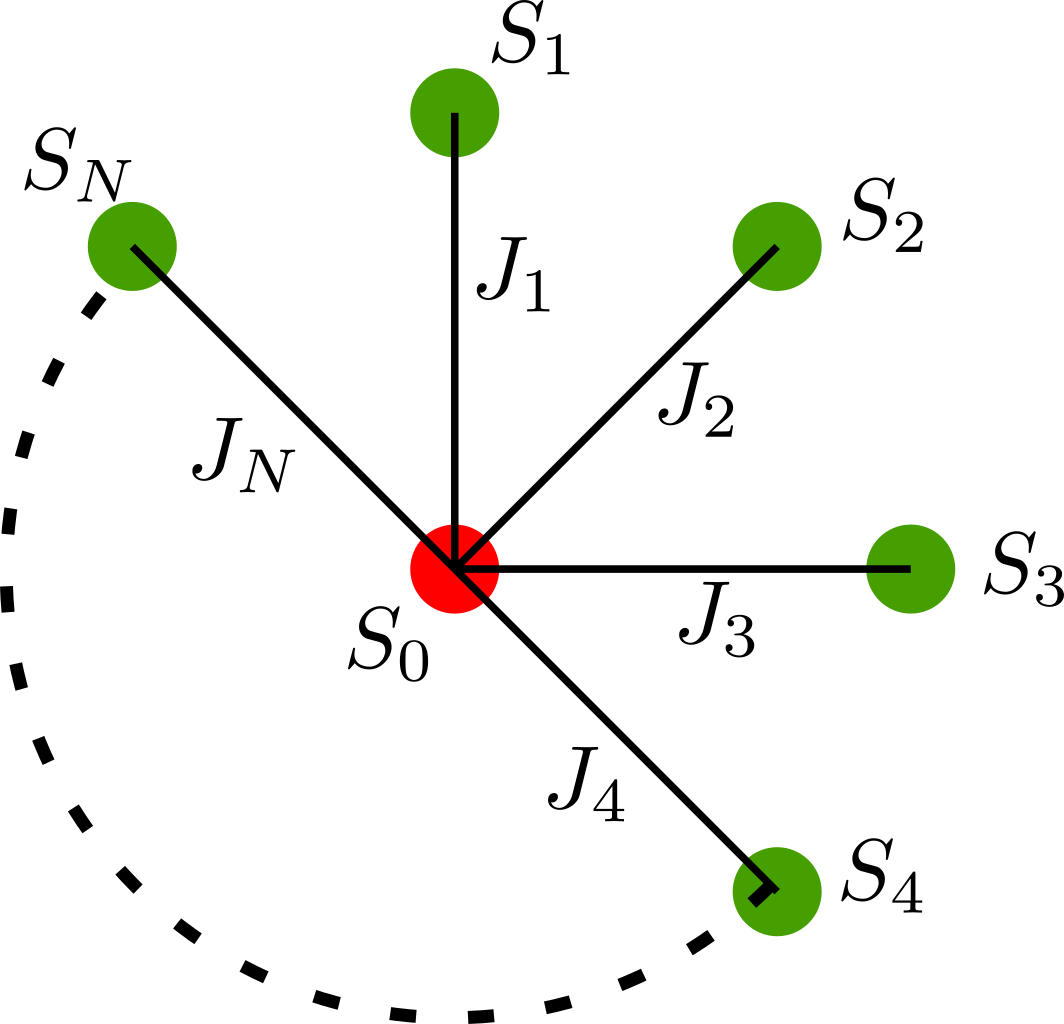
\includegraphics[scale=0.2]{../figures/stargraph_.png}
\captionof{figure}{Star Graph model}
\end{center}
\end{minipage}
\\\\By converting the last term into \(S^z\) and \(S^\pm\), we can write the Hamiltonian as
\begin{equation}\begin{aligned}
	\mathcal{H} = \epsilon_0 S^z_0 + \sum_{i=1}^N\left[\epsilon_i S^z_i + J_i\left(S^z_0 S^z_i + \frac{1}{2}\left(S_0^+ S^-_i + S_0^- S^+_i\right)\right)\right]
\end{aligned}\end{equation}
The diagonal terms are the ones that preserve the number or (in this case) spin.
\begin{equation}\begin{aligned}
\mathcal{H}^d =\sum_{i=0}^N \epsilon_i S^z_i + \sum_{i=1}^N J_iS^z_0 S^z_i 
\end{aligned}\end{equation}
This is the piece that comes in the denominator. The off-diagonal terms are the ones that change the number or spin. For this problem, they are the last two terms, \(S_0^+ S_i^-\) and \(S_0^- S_i^+\).
\\\\The RG involves decoupling the nodes \(N\) through 1, and looking at the resultant renormalization in \(\epsilon_i\) and \(J_i\). As a simplification, we will ignore the lower nodes in the denominator and keep only the node currently being decoupled, ie node \(N\). Since node \(0\) is connected to node \(N\), we will keep node \(0\) in the denominator as well. Making this simplification gives
\begin{equation}\begin{aligned}
	\label{stardiag}
\mathcal{H}^D =\epsilon_0 S^z_0 + \epsilon_N S^z_N + J_NS^z_0 S^z_N 
\end{aligned}\end{equation}
The off-diagonal part in the subspace of the node \(N\) is
\begin{equation}\begin{aligned}
\mathcal{H}_X = \frac{1}{2}J_N \left(S_N^+ S_0^- + S_N^- S_0^+\right)
\end{aligned}\end{equation}
\subsection{Calculation of Renormalization}
The renormalization on doing one step of the URG is given by
\begin{equation}
	\Delta \mathcal{H} = c_{q\beta}^\dagger T \eta + T^\dagger c_{q\beta} \eta_0^\dagger
\end{equation}
There, \(q\beta\) refers to the electron being decoupled. Here, since we are decoupling the spin \(N\), the formula becomes
\begin{equation}
	\Delta \mathcal{H} = \left[S_N^+T,\eta\right]
\end{equation}
where \(S_N^+T\) is the  off-diagonal term in the Hamiltonian and hence \(T\) is  \(S_0^-\). \(\eta\) is of course given by
\begin{equation}
	\eta = \frac{1}{\omega - \mathcal{H}^d}T^\dagger c_{q\beta} \to \frac{1}{\omega - \mathcal{H}^d}\frac{1}{2}J_N S_0^+ S_N^-
\end{equation}
and
\begin{equation}
	\eta_0^\dagger = \frac{1}{\omega^\prime - \mathcal{H}^d}\frac{1}{2}J_N S_N^+ S_0^-
\end{equation}
Substituting the expression for the diagonal part \(\mathcal{H}_d\), we get
\begin{equation}
	\label{stareta}
	\eta  = \frac{1}{\omega - \epsilon_0 S^z_0 - \epsilon_N S^z_N - J_NS^z_0 S^z_N}\frac{1}{2}J_NS_0^+ S_N^- = \frac{1}{\omega - \frac{1}{2}\epsilon_0 + \frac{1}{2}\epsilon_N + \frac{1}{4}J_N}\frac{1}{2}J_NS_0^+ S_N^-
\end{equation}
and
\begin{equation}
	\eta_0^\dagger = \frac{1}{\omega^\prime - \epsilon_0 S^z_0 - \epsilon_N S^z_N - J_NS^z_0 S^z_N}\frac{1}{2}J_NS_N^+ S_0^- = \frac{1}{\omega + \frac{1}{2}\epsilon_0 - \frac{1}{2}\epsilon_N + \frac{1}{4}J_N}\frac{1}{2}J_NS_N^+ S_0^-
\end{equation}
In the final steps, I substituted \(S_N^z = -\frac{1}{2}\) and \(S_0^z = \frac{1}{2}\) in the denominator of \(\eta\), and the opposite values in the denominator of \(\eta_0^\dagger\), because there is \(S_0^+ S_N^-\)(\(S_N^+ S_0^-\)) in front of the Greens function of \(\eta\) (\(\eta_0^\dagger\)). The renormalization thus becomes
\begin{equation}
	\Delta \mathcal{H} = \frac{1}{4}J_N^2 S_N^+S_0^- \frac{1}{\omega - \frac{1}{2}\epsilon_0 + \frac{1}{2}\epsilon_N + \frac{1}{4}J_N}S_0^+ S_N^- + \frac{1}{4}J_N^2S_0^+ S_N^- \frac{1}{\omega^\prime + \frac{1}{2}\epsilon_0 - \frac{1}{2}\epsilon_N + \frac{1}{4}J_N} S_N^+S_0^-
\end{equation}
To compare \(\omega\) and \(\omega^\prime\), we will write down their Poor Man' Scaling counterparts.
\begin{equation}\begin{aligned}
	\omega &= \frac{1}{2}\epsilon_N - \frac{1}{2}\epsilon_0 - \frac{1}{4}J_N\\
	\omega^\prime &= \frac{1}{2}\epsilon_0 - \frac{1}{2}\epsilon_N - \frac{1}{4}J_N = -\omega - \frac{1}{2}J_N
\end{aligned}\end{equation}
So, the renormalization becomes
\begin{equation}
	\Delta \mathcal{H} = \frac{1}{4}J_N^2 \frac{1}{\omega - \frac{1}{2}\epsilon_0 + \frac{1}{2}\epsilon_N + \frac{1}{4}J_N}\left[S_N^+S_0^- S_0^+ S_N^- + S_0^+ S_N^- S_N^+S_0^-\right]
\end{equation}
Using the relations \(S^+ S^- = \frac{1}{2} + S^z\) and \(S^- S^+ = \frac{1}{2} - S^z\), we can write this as
\begin{equation}\begin{aligned}
	\Delta \mathcal{H} &= \frac{1}{4}J_N^2 \frac{1}{\omega - \frac{1}{2}\epsilon_0 + \frac{1}{2}\epsilon_N + \frac{1}{4}J_N}\left[\left(\frac{1}{2} + S_N^z\right)\left(\frac{1}{2} - S_0^z\right) - \left(\frac{1}{2} - S_N^z\right)\left(\frac{1}{2} + S_0^z\right)\right]\\
		    &= \frac{1}{4}J_N^2 \frac{1}{\omega - \frac{1}{2}\epsilon_0 + \frac{1}{2}\epsilon_N + \frac{1}{4}J_N}\left[S_N^z - S_0^z\right]
\end{aligned}\end{equation}
We can now read off the renormalizations in \(\epsilon_N\) and \(\epsilon_0\).
\begin{equation}\begin{aligned}
	\Delta \epsilon_N &= \frac{1}{4}J_N^2 \frac{1}{\omega - \frac{1}{2}\epsilon_0 + \frac{1}{2}\epsilon_N + \frac{1}{4}J_N}\\
	\Delta \epsilon_0 &= -\frac{1}{4}J_N^2 \frac{1}{\omega - \frac{1}{2}\epsilon_0 + \frac{1}{2}\epsilon_N + \frac{1}{4}J_N}
\end{aligned}\end{equation}
\subsection{Nature of flows}
We are interested in looking at the renormalization of the central node energy \(\epsilon_0\), upon removing the nodes \(N\) through 1. We will hence concentrate on the second RG equation. We first make some simplifying assumptions: \(J_i = J, \epsilon_i = \epsilon\) for all \(i\in\{1,N\}\).
\begin{equation}\begin{aligned}
	\label{stareq}
	\Delta \epsilon_0 &= -\frac{1}{4}J^2 \frac{1}{\omega - \frac{1}{2}\epsilon_0 + \frac{1}{2}\epsilon + \frac{1}{4}J}
\end{aligned}\end{equation}
Define \(\tilde\omega = \omega + \frac{1}{2}\epsilon + \frac{1}{4}J\).
\begin{equation}\begin{aligned}
	\Delta \epsilon_0 &= -\frac{1}{4}J^2 \frac{1}{\tilde \omega - \frac{1}{2}\epsilon_0}
\end{aligned}\end{equation}
Our goal here is to look for a fixed-point condition such that the denominator vanishes at some point of the RG. If we start with a bare of \(\epsilon_0\) such that \(\tilde \omega - \frac{1}{2}\epsilon_0 > 0\), the denominator will be positive and the RG equation will be irrelevant. This means that \(\epsilon_0\) will keep on decreasing, and the denominator will keep on becoming more and more positive, meaning there cannot be a fixed point in this situation.
\\\\If, on other hand, we start with a bare of \(\epsilon_0\) such that \(\tilde \omega - \frac{1}{2}\epsilon_0 < 0\), the denominator will be negative and the RG equation will be relevant. This means that \(\epsilon_0\) will keep on increasing, and the denominator will keep on becoming more and more negative, meaning there cannot be a fixed point in this situation either. These situations are depicted in figure \ref{star1}.
\begin{figure}
	\centering
	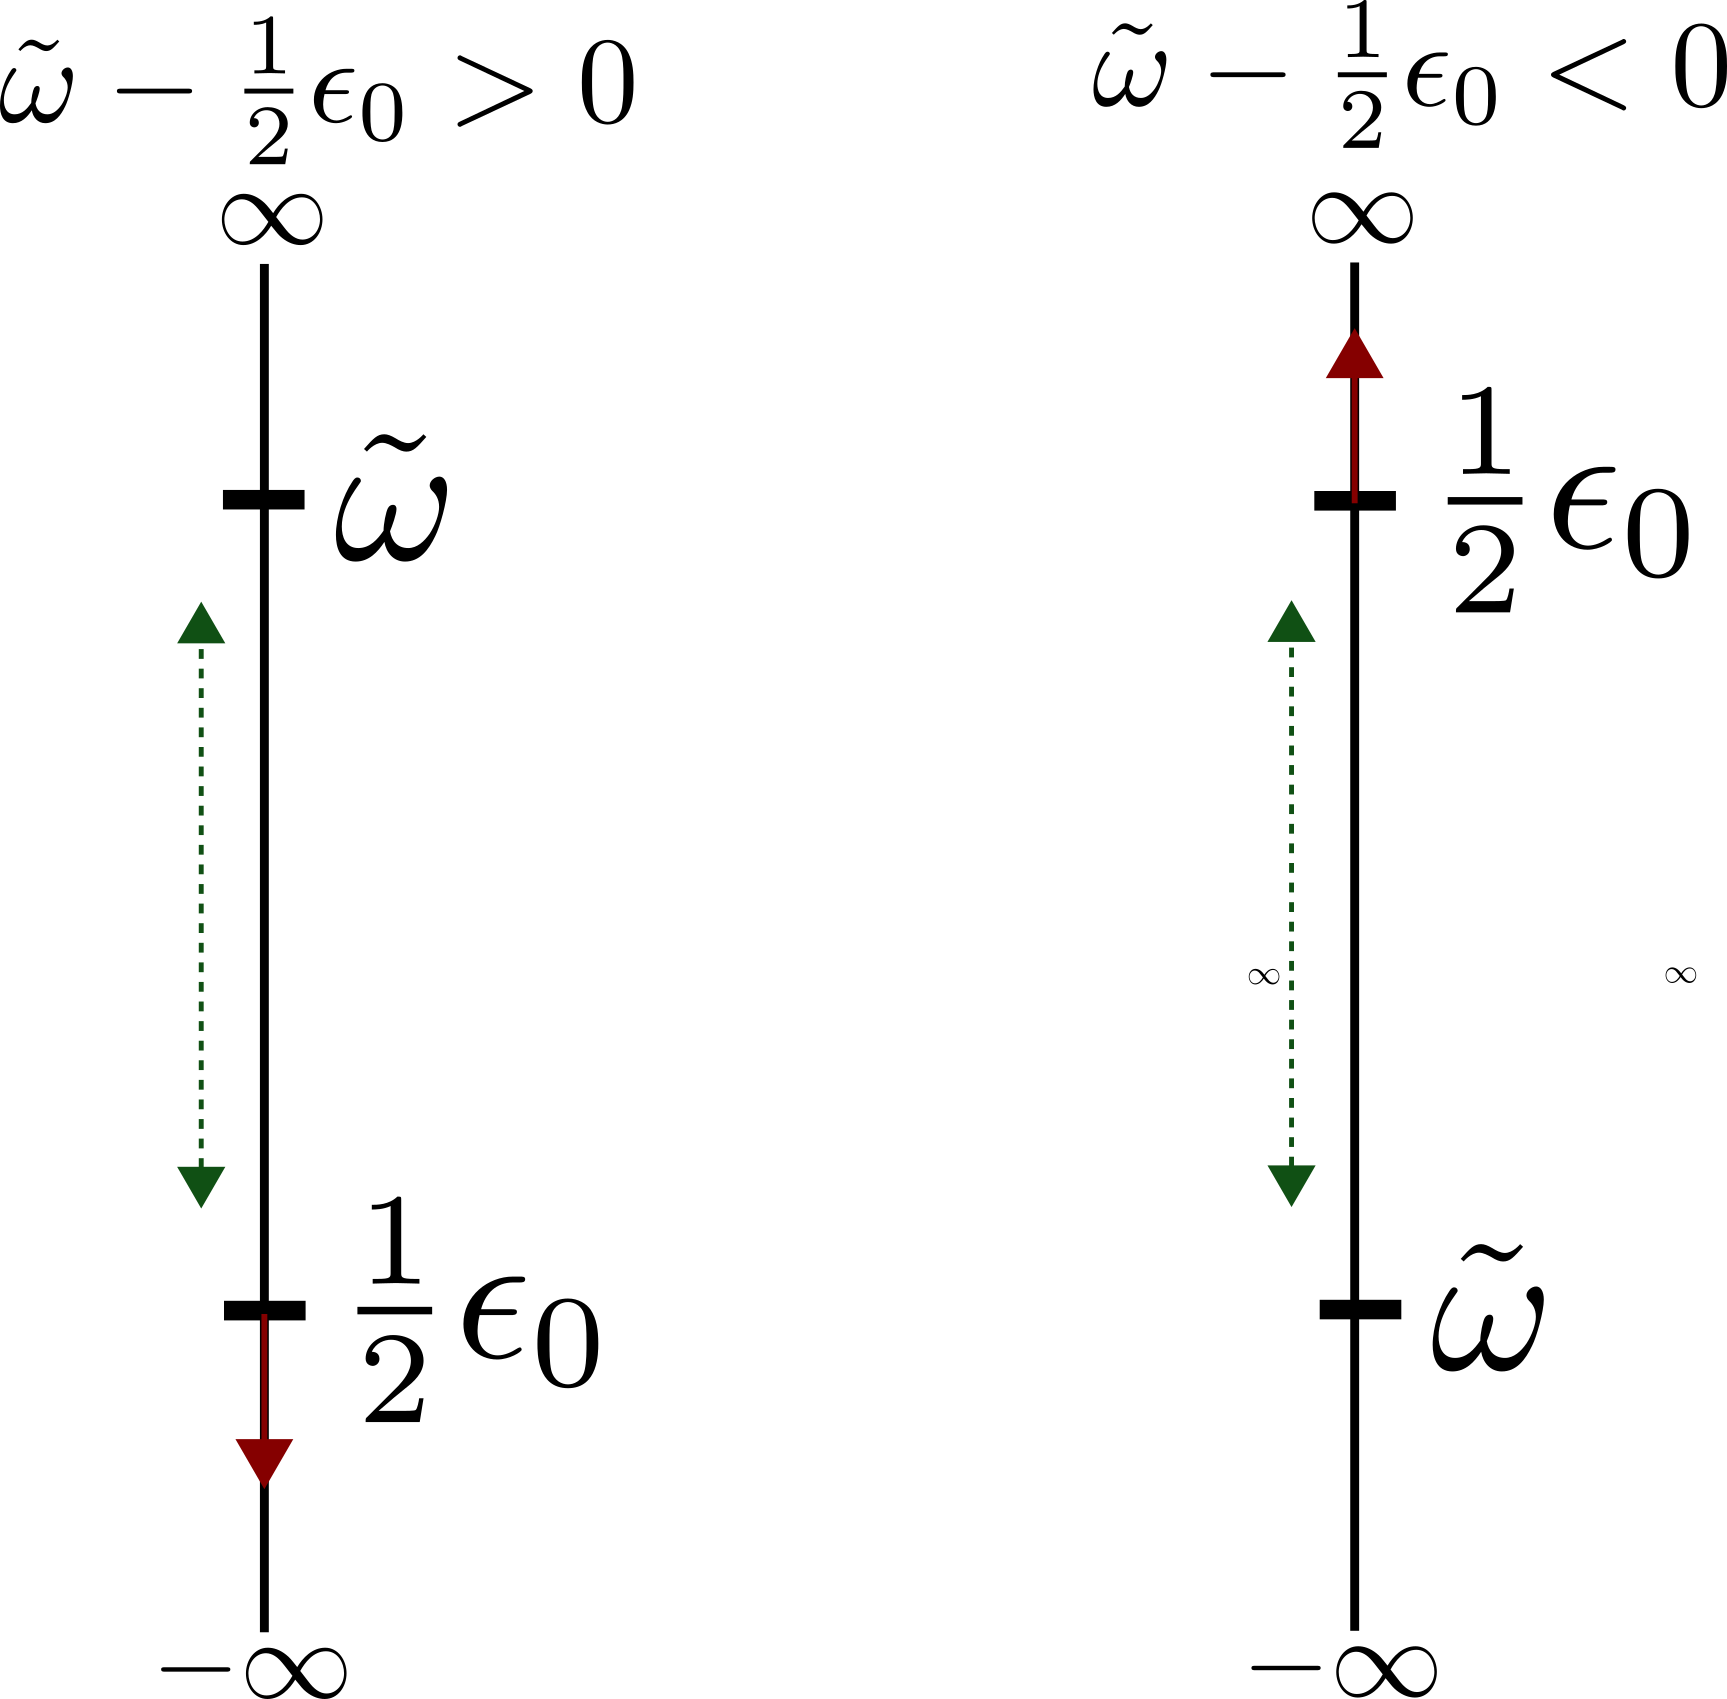
\includegraphics[scale=0.4]{star}
	\captionof{figure}{RG flow for the two cases. The green line is the distance between the bare values of the two couplings, and hence also the magnitude of the denominator. The red arrow denotes the direction in which \(\epsilon_0\) will flow. Upward flow is increase. In both cases, the flow is such that the distance between the two quantities (and hence the magnitude of the denominator) increases. The RG fixed point occurs when the magnitude of the denominator goes to 0. This happens if the distance vanishes. Since the distance necessarily increases, we cannot get a fixed point in this way.}
	\label{star1}
	\vspace*{\fill}
	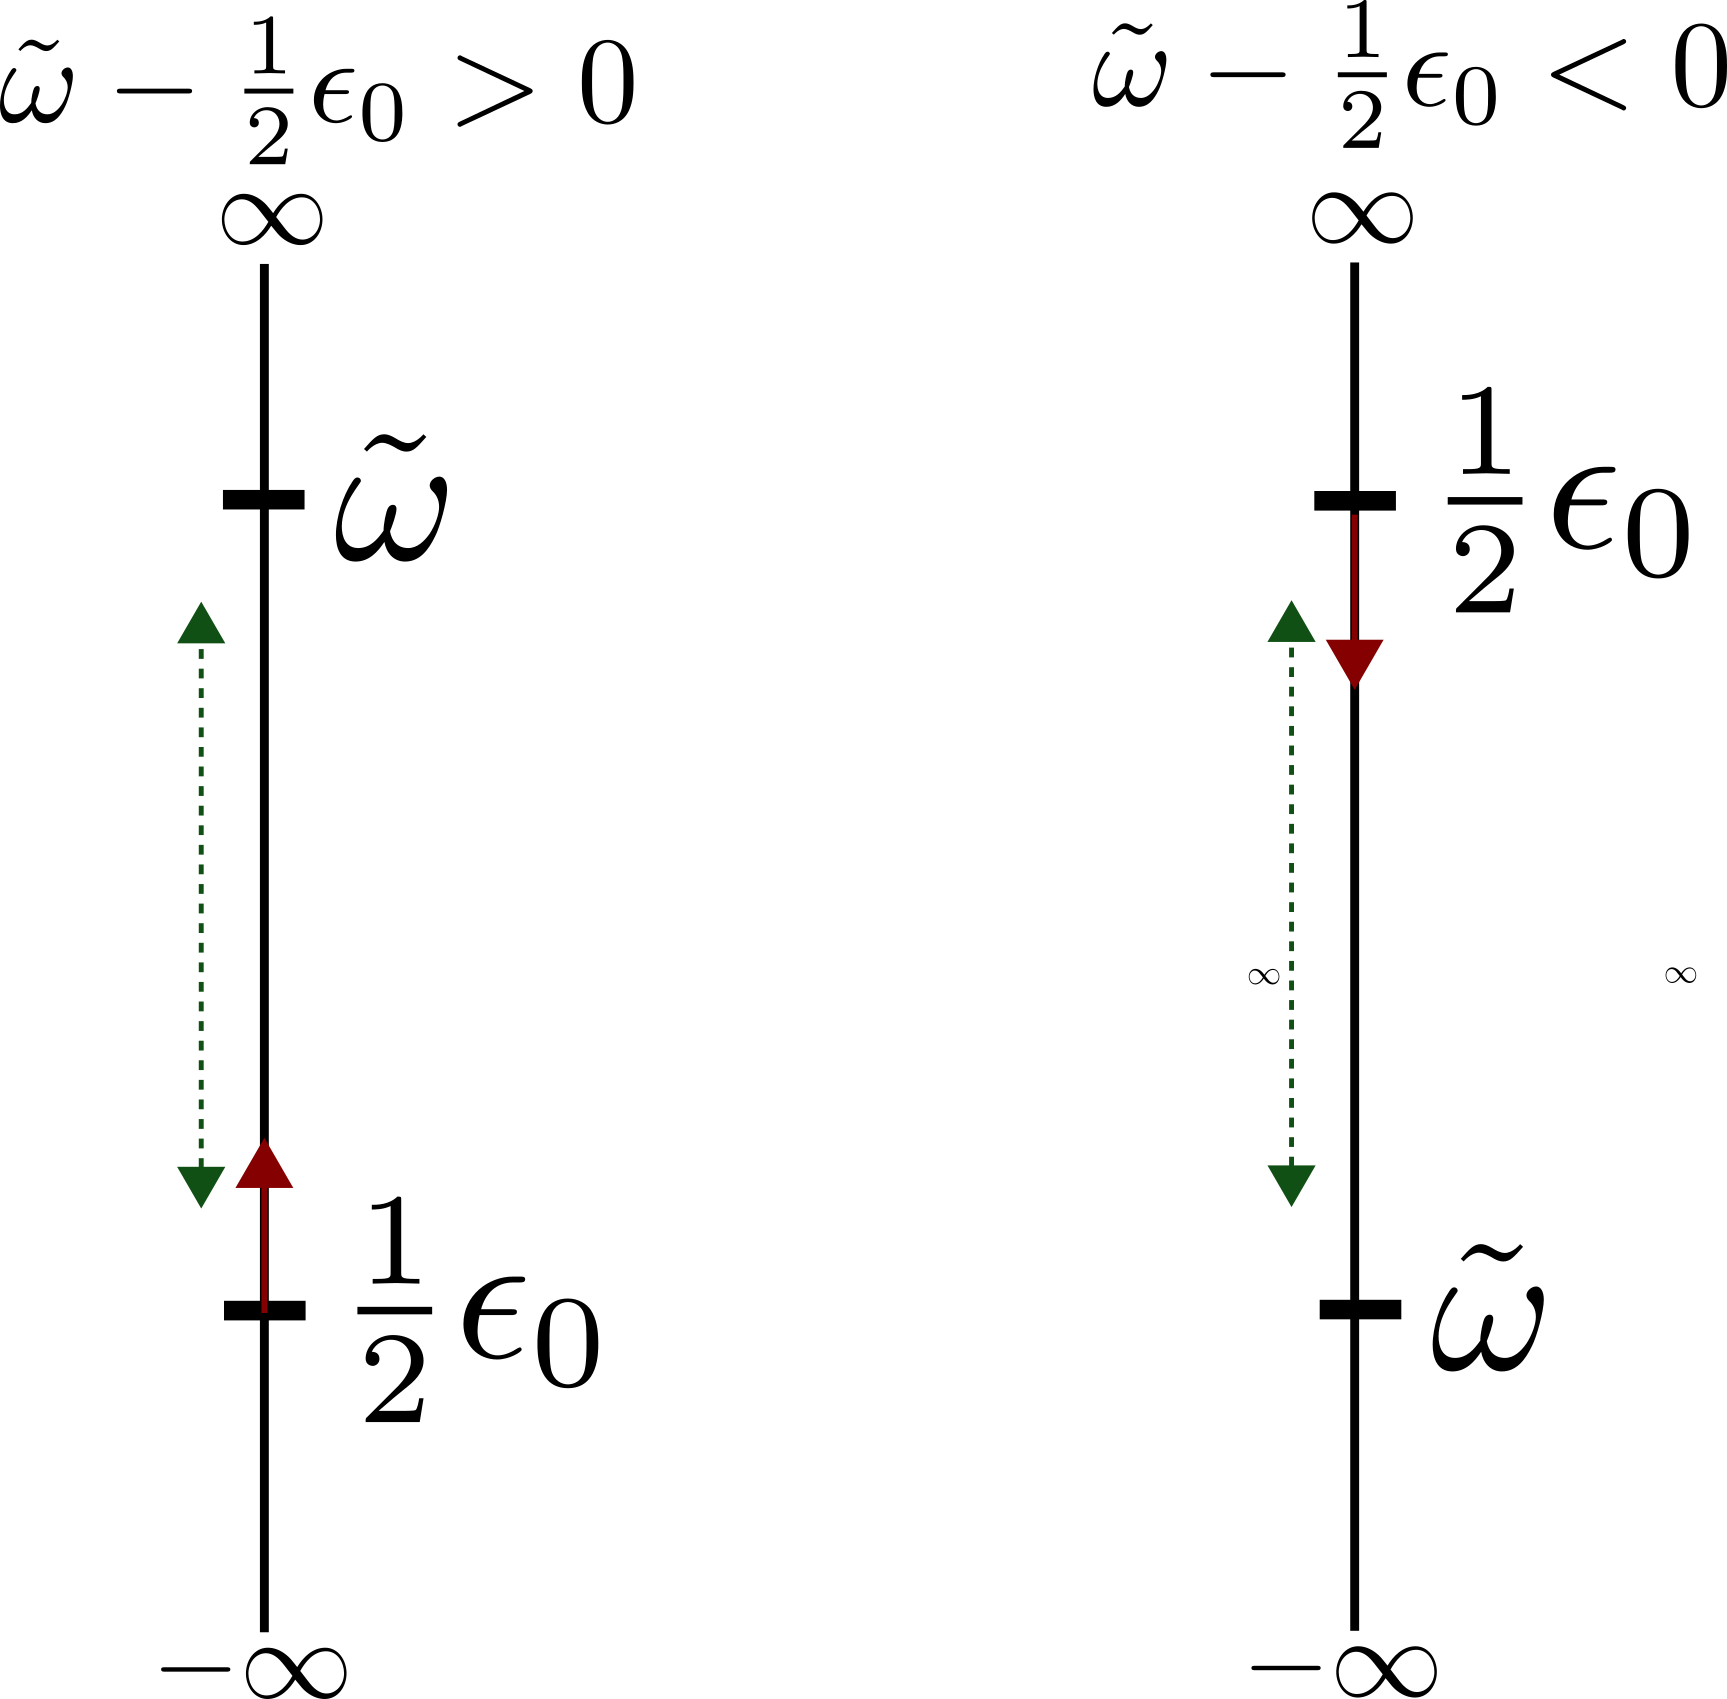
\includegraphics[scale=0.4]{star3}
	\label{star3}
	\captionof{figure}{RG flow for the two cases with the new \(-\tilde \omega = \omega^\prime - \frac{1}{2}\epsilon + \frac{1}{4}J\). Now we can see that in both cases, the flow is such that the distance (green dotted line) between the couplings decreases. A fixed point is reached when this distance vanishes.}
\end{figure}
\\\\Since we cannot find a fixed point, we will use the other \(\omega\) in the URG formalism. Recall that \(\eta\) and \(\eta^\dagger\) will, in general, have different \(\omega\), eq.~\ref{etadefine}.
\begin{equation}
	\eta^\dagger = \frac{1}{\omega^\prime - \mathcal{H}_d}S_N^+ S_0^- = \frac{1}{\omega^\prime - \frac{1}{2}\epsilon + \frac{1}{2}\epsilon_0 + \frac{1}{4}J}S_N^+ S_0^-
\end{equation}
Comparing with eq.~\ref{stareta}, and requiring \(\left(\eta\right)^\dagger = \eta^\dagger\), we get the following equation relating \(\omega\) and \(\omega^\prime\):
\begin{equation}
	\omega^\prime - \frac{1}{2}\epsilon + \frac{1}{2}\epsilon_0 + \frac{1}{4}J = \omega + \frac{1}{2}\epsilon - \frac{1}{2}\epsilon_0 + \frac{1}{4}J \implies \omega = \omega^\prime - \epsilon + \epsilon_0
\end{equation}
Substituting this in eq.~\ref{stareq} gives
\begin{equation}\begin{aligned}
	\Delta \epsilon_0 = -\frac{1}{4}J^2 \frac{1}{\omega^\prime - \frac{1}{2}\epsilon + \frac{1}{2}\epsilon_0 + \frac{1}{4}J}
\end{aligned}\end{equation}
We again define \(-\tilde \omega = \omega^\prime - \frac{1}{2}\epsilon + \frac{1}{4}J\).
\begin{equation}\begin{aligned}
	\Delta \epsilon_0 = \frac{1}{4}J^2 \frac{1}{\tilde \omega - \frac{1}{2}\epsilon_0}
\end{aligned}\end{equation}
We now repeat the exercise of determining the relevance of the flows under various regime. If we start with a bare \(\epsilon_0\) such that \(\tilde \omega + \frac{1}{2}\epsilon_0 > 0\), then the denominator is positive so the renormalization will be irrelevant. \(\epsilon_0\) will decrease until we reach \(\tilde \omega + \frac{1}{2}\epsilon_0 = 0\). This will be a fixed point. However, if we start with a bare \(\epsilon_0\) such that \(\tilde \omega + \frac{1}{2}\epsilon_0 < 0\), then the denominator is negative so the renormalization will be relevant. \(\epsilon_0\) will increase until we reach \(\tilde \omega + \frac{1}{2}\epsilon_0 = 0\). This will again be a fixed point. This new situation is depicted in figure \ref{star3}.
%\begin{center}
%\end{center}
\subsection{Effective Hamiltonians}
If \(\tilde\omega\) and \(\epsilon_0\) are of the same sign at the bare level, then it is easy to see that since the fixed point is defined by \(\tilde\omega = \frac{1}{2}\epsilon_0^*\) (* denotes value at fixed point), the effective Hamiltonian at the fixed point will be
\begin{equation}\begin{aligned}
	\mathcal{H}^* = 2\tilde\omega S_0^z +  \epsilon \sum_i S_i^z + J\sum_i \vec S_i \cdot \vec S_0, && \text{ if }\tilde\omega \epsilon_0 > 0
\end{aligned}\end{equation}
If, at the bare level, \(\epsilon_0\) and \(\tilde\omega\) are of opposite signs, then \(\epsilon_0\) would undergo a change in sign at some point as it flows towards \(\tilde \omega\). Since we do not expect a coupling to change sign under RG, we will restrict it to 0 in such cases.
\begin{equation}\begin{aligned}
	\mathcal{H}^* = \epsilon \sum_i S_i^z + J\sum_i \vec S_i \cdot \vec S_0, && \text{ if }\tilde\omega \epsilon_0 < 0
\end{aligned}\end{equation}
Things get much more simpler if we assume the onsite energies of the surrounding nodes are zero.
\begin{equation}\begin{aligned}
	\mathcal{H}^* &= 2\tilde\omega S_0^z + J\sum_i \vec S_i \cdot \vec S_0, && \text{ if }\tilde\omega \epsilon_0 > 0\\
	\mathcal{H}^* &= J\sum_i \vec S_i \cdot \vec S_0, && \text{ if }\tilde\omega \epsilon_0 < 0
\end{aligned}\end{equation}
\subsection{Fixed points}
The fixed points are obtained numerically by solving the RG equation. As mentioned before, there are two types of solutions: The first kind is those in which \(\epsilon_0\) and \(\tilde \omega\) are of the same sign, and the former flows to the latter without crossing the 0 axis. These flows are shown (obtained numerically) in fig.~\ref{plot1}. The second kind are those where the two couplings have different signs, and so \(\epsilon_0\) flows to 0. These are shown in fig.~\ref{plot2}.
\begin{center}
	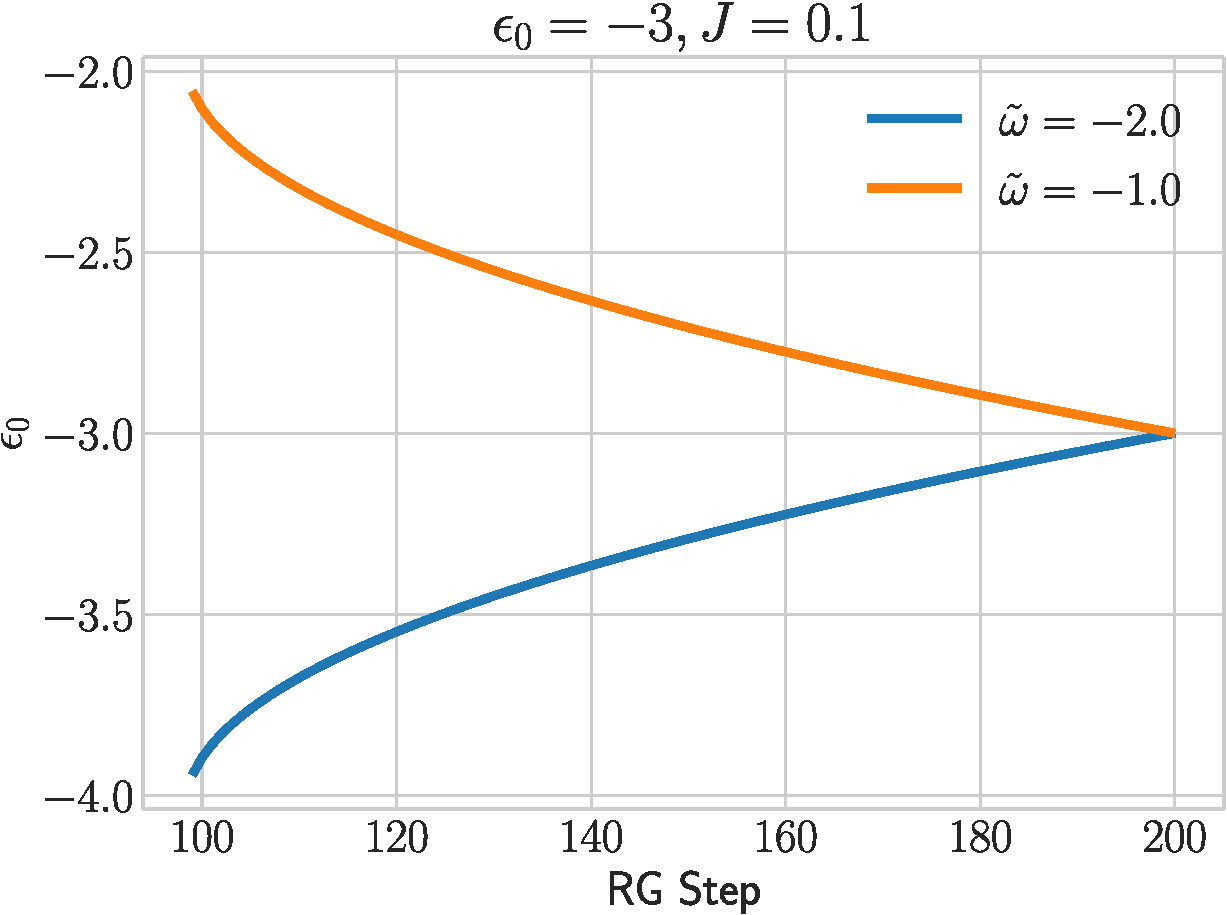
\includegraphics[width=0.45\textwidth]{../figures/notzero1.pdf}
	\hspace*{\fill}
	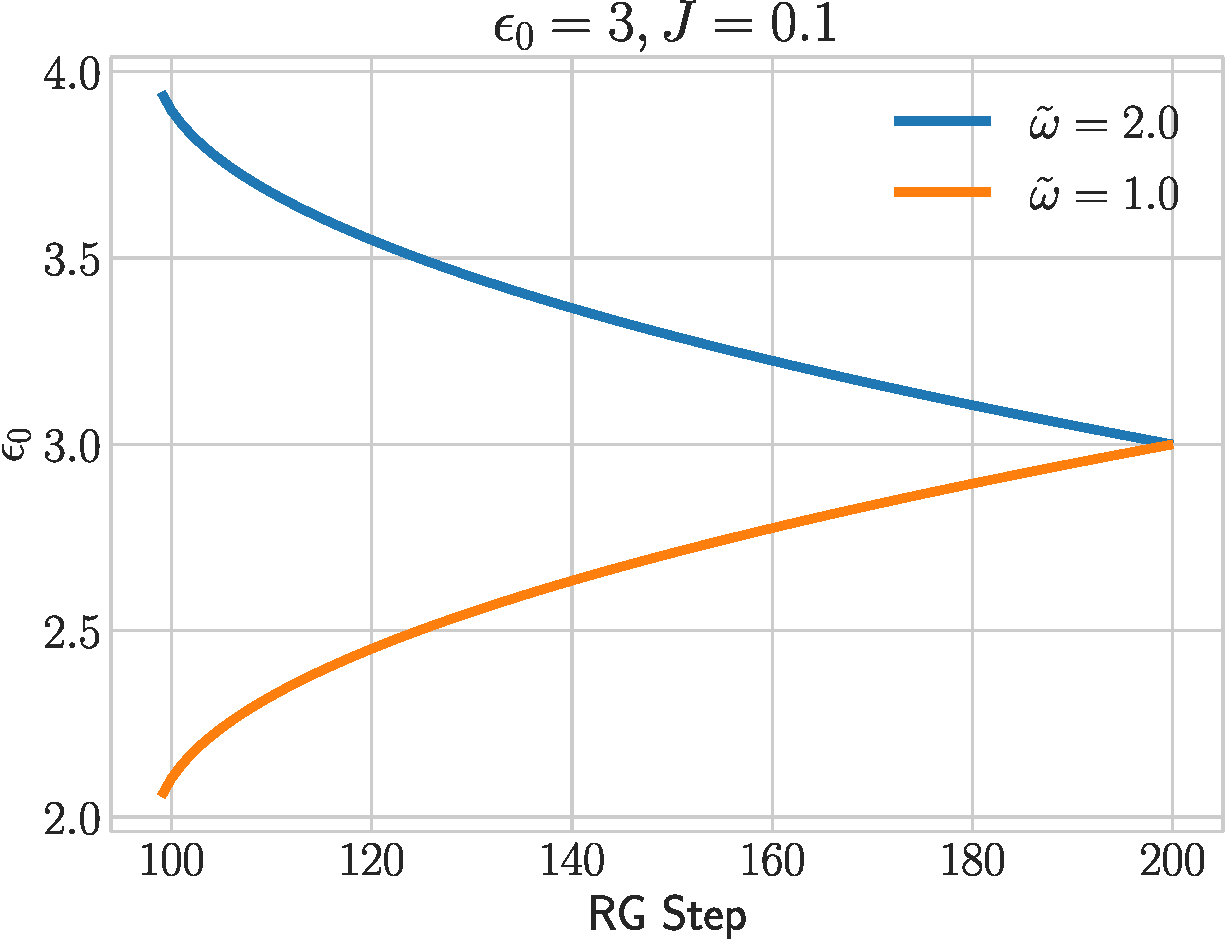
\includegraphics[width=0.45\textwidth]{../figures/notzero2.pdf}
	\captionof{figure}{Flows where \(\epsilon_0\) and \(\tilde\omega\) have same sign. The left and right panels show flows starting from negative and positive values respectively. The two plots in each panel correspond to different values of \(\tilde \omega\), one greater than the bare \(\epsilon_0\), the other less than that. The fixed point value is \(2\tilde\omega\).}
	\label{plot1}
\end{center}
\begin{center}
	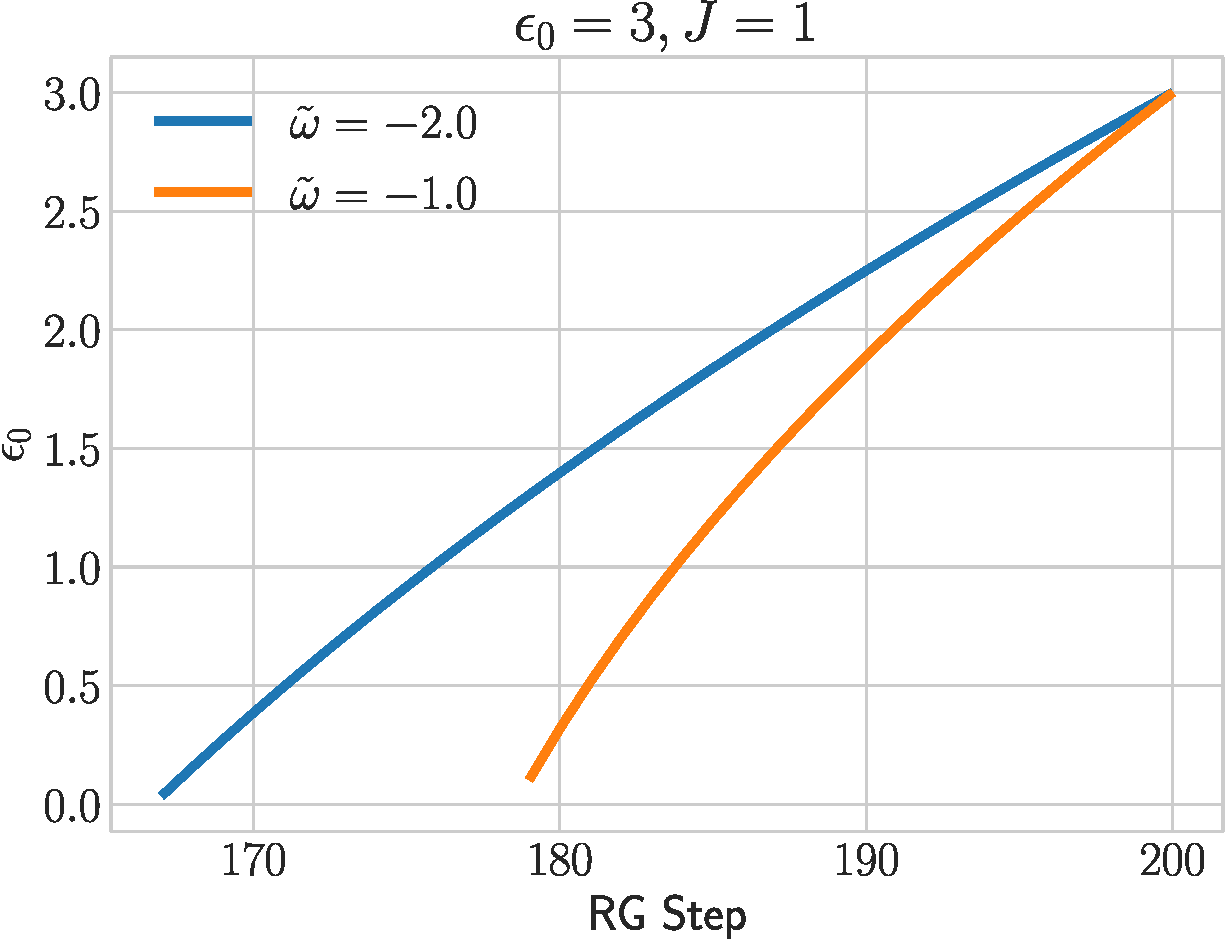
\includegraphics[width=0.45\textwidth]{../figures/zero2.pdf}
	\hspace*{\fill}
	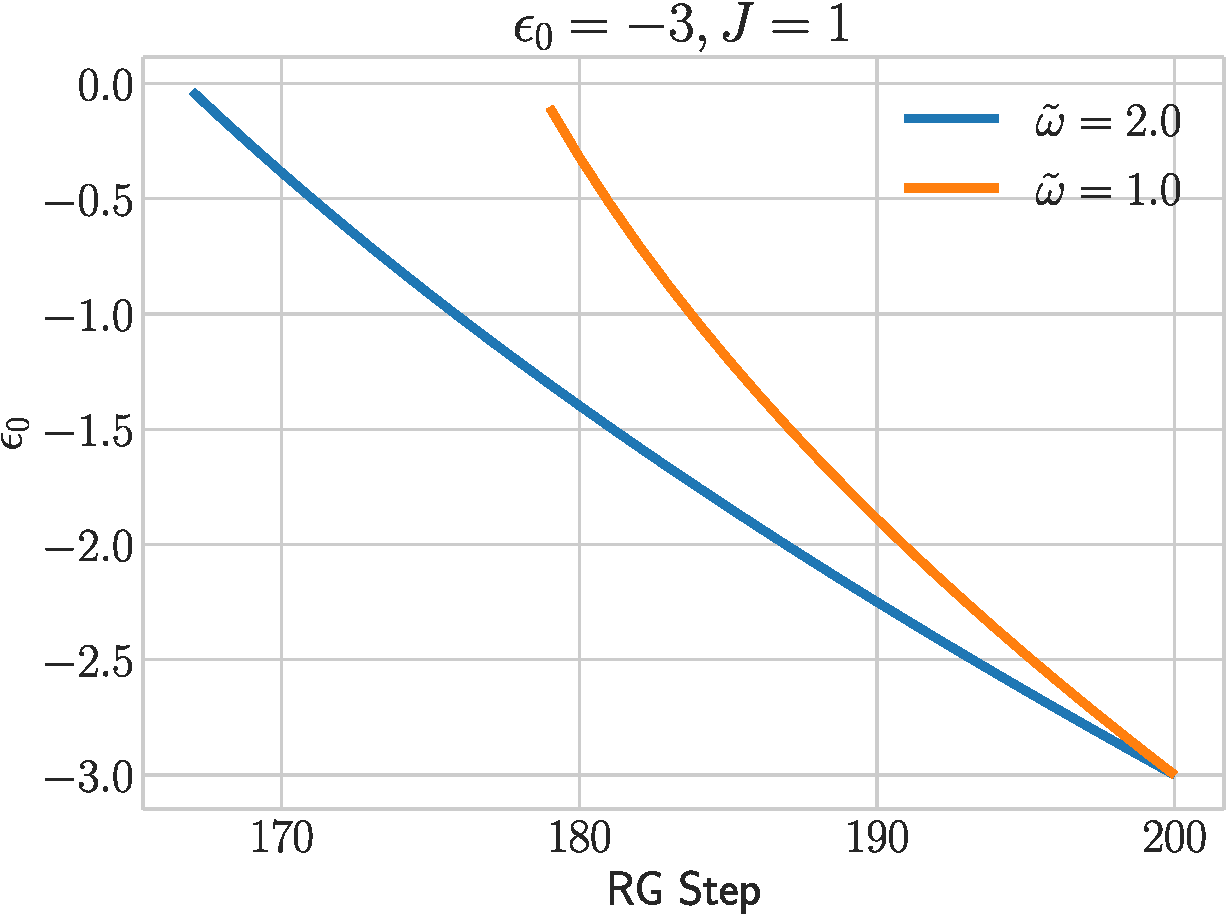
\includegraphics[width=0.45\textwidth]{../figures/zero1.pdf}
	\captionof{figure}{Flows where \(\epsilon_0\) and \(\tilde\omega\) have opposite sign. The left and right panels show flows starting from negative and positive values respectively. The two plots in each panel correspond to different values of \(\tilde \omega\), one greater than the bare \(\epsilon_0\), the other less than that. The fixed point value is 0.}
	\label{plot2}
\end{center}
\section{Kondo Model URG}
\label{kondourg}
The Kondo model URG analysis is first carried out in ref.~\cite{am_thesis}. The model is of course described by the Hamiltonian
\begin{equation}\begin{aligned}
	\mathcal{H} = \sum_{k\alpha}\epsilon_{k}\hat n_{k\alpha} + J_z\sum_{k,k^\prime} S_d^z\left(c^\dagger_{k\uparrow}c_{k^\prime\uparrow} - c^\dagger_{k\downarrow}c_{k^\prime\downarrow}\right) + J_t\sum_{k,k^\prime}\left(S_d^+ c^\dagger_{k\downarrow}c_{k^\prime\uparrow} + S_d^- c^\dagger_{k\uparrow}c_{k^\prime\downarrow}\right)
\end{aligned}\end{equation}
The goal is to disentangle an electron \(q\beta\) from the Hamiltonian, \(q\) being the momentum and \(\beta\) the spin. The diagonal part of the Hamiltonian is
\begin{equation}\begin{aligned}
	\mathcal{H}_d = \epsilon_q \hat n_{q\beta} + J_z S_d^z \beta\left(\hat n_{q\beta} - \hat n_{q\overline\beta}\right)
\end{aligned}\end{equation}
Note that we keep only those terms in the diagonal part that relate to either the impurity or the electron we are disentangling-\(q\beta\). This piece \(\mathcal{H}_d\) is the one that comes in the denominator. Note that in this form, the hole energy comes out to be zero, because the Hamiltonian is written only in terms of \(\hat n_{q\beta}\). To remedy this, we write the Hamiltonian in terms of \(\tau_{q\beta} = \hat n_{q\beta} - \frac{1}{2}\).
\begin{equation}\begin{aligned}
	\label{kondodiag}
\mathcal{H}_d = \epsilon_q \tau_{q\beta} + J_z S_d^z \beta \hat n_{q\beta}
\end{aligned}\end{equation}
A constant \(\frac{1}{2} \epsilon_q\) has been dropped while transforming the first term.
\\\\The off-diagonal part involving the electron on the shell is
\begin{equation}\begin{aligned}
	\mathcal{H}^I = J_z\sum_{k}S^z_d\beta\left(c^\dagger_{k\beta}c_{q\beta} +  c^\dagger_{q\beta}c_{k\beta}\right) + J_t \sum_{k}\left(c^\dagger_{d\beta}c_{d\overline\beta} c^\dagger_{k\overline\beta}c_{q\beta} + c^\dagger_{b\overline\beta}c_{d\beta} c^\dagger_{q\beta}c_{k\overline\beta}\right)
\end{aligned}\end{equation}
These are the terms that come in the numerator.
\subsection{Particle sector}
The particle sector involves integrating out those states which are occupied (\(\hat n_{q\beta}=1\)). We will work at a shell with energy \(-\epsilon_q\).
\begin{equation}\begin{aligned}
	c^\dagger_{q\beta}T \eta
\end{aligned}\end{equation}
where
\begin{equation}\begin{aligned}
	\label{partomega}
	\eta &= \frac{1}{\omega - \mathcal{H}_d} \left[ J_z\sum_k \beta S_d^z c^\dagger_{k\beta}c_{q\beta} + J_t \sum_k c^\dagger_{d\beta}c_{d\overline\beta} c^\dagger_{k\overline\beta}c_{q\beta} \right]\\
	     &=\sum_k \left[\frac{1}{\hat \omega_1 - \hat E_1 } J_z S_d^z \beta c^\dagger_{k\beta}c_{q\beta} + \frac{1}{\omega_3 - E_3}J_t  c^\dagger_{d\beta}c_{d\overline\beta} c^\dagger_{k\overline\beta}c_{q\beta}\right] 
\end{aligned}\end{equation}
Noting that \(\beta S_d^z = \frac{1}{2}\left( \hat n_{d\beta} - \hat n_{d\overline\beta} \right) = \frac{1}{2}\hat n_{d\beta}\left( 1 - \hat n_{d\overline\beta} \right) - \frac{1}{2}\hat n_{d\overline\beta}\left( 1 - \hat n_{d\beta} \right)\), we can write the \(\eta\) as
\begin{equation}\begin{aligned}
	     \sum_k \left[\frac{ J_z \frac{1}{2}\hat n_{d\beta}\left( 1 - \hat n_{d\overline\beta} \right) c^\dagger_{k\beta}c_{q\beta}}{\omega_1 - E_1} - \frac{J_z \frac{1}{2}\hat n_{d\overline\beta}\left( 1 - \hat n_{d\beta} \right) c^\dagger_{k\beta}c_{q\beta}}{\omega_2 - E_2} + \frac{J_t  c^\dagger_{d\beta}c_{d\overline\beta} c^\dagger_{k\overline\beta}c_{q\beta}}{\omega_3 - E_3}\right] 
\end{aligned}\end{equation}
The energies \(E_i\) now need to be determined. For the last term, it is obvious:
\begin{equation}\begin{aligned}
	E_3 = \frac{1}{2}\epsilon_q - \frac{1}{2}J_z
\end{aligned}\end{equation}
For the first two term, note that these terms do not flip the spin; hence, the denominator should reflect that. The total magnetization for the spin \(\beta\) in the initial state is \(\hat n_\beta = \hat n_{q\beta} = 1\), because of the \(q\beta\). It is also \(1\) in the intermediate state, because of the spin \(k\beta\): \(\hat n_\beta = \hat n_{k\beta} = 1\). This holds for both \(E_1\) and \(E_2\). The impurity magnetization is however \(1\) in the first term but \(-1\) in the second term. Hence,
\begin{equation}\begin{aligned}
	E_1 &= \frac{1}{2}\epsilon_q + \frac{1}{2}J_z\\
	E_2 &= \frac{1}{2}\epsilon_q - \frac{1}{2}J_z = E_3\\
\end{aligned}\end{equation}
To relate the \(\omega_i\), we will use their diagonal values. By replacing them with the initial state energies, we can write
\begin{equation}\begin{aligned}
	\omega_1 = - \frac{1}{2}\epsilon_q + \frac{1}{2}J_z\\
	\omega_2 = \omega_3 = - \frac{1}{2}\epsilon_q - \frac{1}{2}J_z\\
\end{aligned}\end{equation}
Defining \(\omega \equiv \omega_3\), we can write \(\omega_1 = \omega + J_z\) and \(\omega_2 = \omega\). Therefore,
\begin{equation}\begin{aligned}
	\eta = \sum_k \left[\frac{ J_z \frac{1}{2}\hat n_{d\beta}\left( 1 - \hat n_{d\overline\beta} \right) c^\dagger_{k\beta}c_{q\beta}}{\xi_1} - \frac{J_z \frac{1}{2}\hat n_{d\overline\beta}\left( 1 - \hat n_{d\beta} \right) c^\dagger_{k\beta}c_{q\beta}}{\xi_2} + \frac{J_t  c^\dagger_{d\beta}c_{d\overline\beta} c^\dagger_{k\overline\beta}c_{q\beta}}{\xi_3}\right] 
\end{aligned}\end{equation}
where \(\xi_i \equiv \omega_i - E_i\), hence
\begin{equation}\begin{aligned}
	\xi_1 = \xi_2 = \xi_3 = \omega - \frac{1}{2}\epsilon_q + \frac{1}{2}J_z \equiv \xi
\end{aligned}\end{equation}
Therefore,
\begin{equation}\begin{aligned}
	\eta &= \frac{1}{\xi}\sum_k \left[ J_z \frac{1}{2}\hat n_{d\beta}\left( 1 - \hat n_{d\overline\beta} \right) c^\dagger_{k\beta}c_{q\beta} - J_z \frac{1}{2}\hat n_{d\overline\beta}\left( 1 - \hat n_{d\beta} \right) c^\dagger_{k\beta}c_{q\beta} + J_t  c^\dagger_{d\beta}c_{d\overline\beta} c^\dagger_{k\overline\beta}c_{q\beta}\right] \\
	     &= \frac{1}{\xi}\sum_k \left[ J_z \frac{1}{2}\left(\hat n_{d\beta} - \hat n_{d\overline\beta}\right) c^\dagger_{k\beta}c_{q\beta} + J_t  c^\dagger_{d\beta}c_{d\overline\beta} c^\dagger_{k\overline\beta}c_{q\beta}\right]\\
	     &= \frac{1}{\xi}\sum_k \left[ J_z \beta S_d^z c^\dagger_{k\beta}c_{q\beta} + J_t  c^\dagger_{d\beta}c_{d\overline\beta} c^\dagger_{k\overline\beta}c_{q\beta}\right]
\end{aligned}\end{equation}
The renormalization is therefore
\begin{equation}\begin{aligned}
	\frac{1}{\xi}\sum_{kk^\prime} \left[J_z \beta S_d^z c^\dagger_{q\beta}c_{k^\prime\beta}\times J_z \beta S_d^z c^\dagger_{k\beta}c_{q\beta} + J_t  c^\dagger_{d\overline\beta}c_{d\beta} c^\dagger_{q\beta}c_{k^\prime\overline\beta} \times J_t  c^\dagger_{d\beta}c_{d\overline\beta} c^\dagger_{k\overline\beta}c_{q\beta}\right.\\
	+\left. J_t  c^\dagger_{d\overline\beta}c_{d\beta} c^\dagger_{q\beta}c_{k^\prime\overline\beta}\times J_z \beta S_d^z c^\dagger_{k\beta}c_{q\beta} + J_z \beta S_d^z c^\dagger_{q\beta}c_{k^\prime\beta}\times J_t  c^\dagger_{d\beta}c_{d\overline\beta} c^\dagger_{k\overline\beta}c_{q\beta}\right]
\end{aligned}\end{equation}
We can see that the total renormalization will have three types of terms: \(J_z^2, J_t^2\) and \(J_z J_t\). We can ignore the \(J_z^2\) term because it has no impurity operator (\({S_d^z}^2 = \frac{1}{4}\)). The remaining terms give
\begin{equation}\begin{aligned}
	\label{kondo_part}
	\frac{1}{\xi}\sum_{kk^\prime} \left[\frac{1}{2} J_z J_t\left(c^\dagger_{d\overline\beta}c_{d\beta}c_{k^\prime\overline\beta}c^\dagger_{k\beta} + \text{h.c.}\right) + J_t^2 \hat n_{d\overline\beta}\left(1 - \hat n_{d\beta}\right) c_{k^\prime\overline\beta}c^\dagger_{k\overline\beta}\right]
\end{aligned}\end{equation}
For the Kondo problem, we are in the subspace of \(\hat n_d= 1\), so we can write
\begin{equation}\begin{aligned}
	\hat n_{d\overline\beta}\left(1 - \hat n_{d\beta}\right) = \left(\frac{1}{2} +  \overline\beta S_d^z \right)
\end{aligned}\end{equation}
and
\begin{equation}\begin{aligned}
	\sum_{kk^\prime}\left( c^\dagger_{d\overline\beta}c_{d\beta}c_{k^\prime\overline\beta}c^\dagger_{k\beta} + \text{h.c.}\right) = -\sum_{kk^\prime}\left( c^\dagger_{d\overline\beta}c_{d\beta}c^\dagger_{k\beta}c_{k^\prime\overline\beta} + \text{h.c.}\right) = -\left(S_d^+ s^- + S_d^- s^+\right)
\end{aligned}\end{equation}
The renormalization then becomes
\begin{equation}\begin{aligned}
	\frac{1}{\xi} \left[-\frac{1}{2} J_z J_t\left(S_d^+ s^- + S_d^- s^+\right) + J_t^2 \left(\frac{1}{2} +  \overline\beta S_d^z \right) \sum_{kk^\prime}c_{k^\prime\overline\beta}c^\dagger_{k\overline\beta}\right]
\end{aligned}\end{equation}

\subsection{Hole sector}
For the hole sector, we will take the configuration where \(\hat n_{q\beta} = 0\) and hence the energy \(\epsilon_q\). The renormalization here is
\begin{equation}\begin{aligned}
	T^\dagger c_{q\beta}\eta^\dagger_0 = T^\dagger c_{q\beta}\frac{1}{\omega^\prime - \mathcal{H}_d}c^\dagger_{q\beta} T
\end{aligned}\end{equation}
where \(\eta_0\) is defined in eq.~\ref{eta0}.
\begin{equation}\begin{aligned}
	\label{holeomega}
	\eta_0^\dagger = \frac{1}{\hat \omega^\prime - \hat E_1}\frac{1}{2}J_z \beta S_d^z c^\dagger_{q\beta}c_{k\beta} + \frac{1}{\omega^\prime - E_3}J_tc^\dagger_{d\overline\beta}c_{d\beta}c^\dagger_{q\beta}c_{k\overline\beta}
\end{aligned}\end{equation}
We once again split the \(S_d^z\) term into two parts, and get
\begin{equation}\begin{aligned}
	\eta^\dagger_0 = \sum_k \left[\frac{ J_z \frac{1}{2}\hat n_{d\beta}\left( 1 - \hat n_{d\overline\beta} \right) c^\dagger_{q\beta}c_{k\beta}}{\xi^\prime_1} - \frac{J_z \frac{1}{2}\hat n_{d\overline\beta}\left( 1 - \hat n_{d\beta} \right) c^\dagger_{q\beta}c_{k\beta}}{\xi^\prime_2} + \frac{J_t  c^\dagger_{d\overline\beta}c_{d\beta} c^\dagger_{q\beta}c_{k\overline\beta}}{\xi^\prime_3}\right] 
\end{aligned}\end{equation}
Calculating the energies gives
\begin{equation}\begin{aligned}
	E^\prime_1 &= \frac{1}{2}\epsilon_q + \frac{1}{2}J_z\\
	E^\prime_2 &= \frac{1}{2}\epsilon_q - \frac{1}{2}J_z = E^\prime_3\\
	\omega^\prime_1 &= - \frac{1}{2}\epsilon_q + \frac{1}{2}J_z = \omega + J_z\\
	\omega^\prime_2 = \omega^\prime_3 &= - \frac{1}{2}\epsilon_q - \frac{1}{2}J_z = \omega\\
	\xi_i^\prime &= \omega - \frac{1}{2}\epsilon_q + \frac{1}{2}J_z = \xi
\end{aligned}\end{equation}
Evaluating the terms similar to the particle sector gives
\begin{equation}\begin{aligned}
	\label{kondo_hole}
	\frac{1}{\xi}\sum_{kk^\prime} \left[ -\frac{1}{2} J_z J_t\left(c^\dagger_{d\overline\beta}c_{d\beta}c^\dagger_{k\beta}c_{k^\prime\overline\beta} + \text{h.c.}\right) + J_t^2 \hat n_{d\beta}\left(1 - \hat n_{d\overline\beta}\right) c^\dagger_{k\overline\beta}c_{k^\prime\overline\beta}\right]
\end{aligned}\end{equation}
\subsection{Scaling equations}
Adding the two sectors (eqs.~\ref{kondo_part} and \ref{kondo_hole}) gives
\begin{equation}\begin{aligned}
	\Delta \mathcal{H} &= \frac{1}{\xi}\sum_{kk^\prime} \left[ - J_z J_t\left(c^\dagger_{d\overline\beta}c_{d\beta}c^\dagger_{k\beta}c_{k^\prime\overline\beta} + \text{h.c.}\right) + J_t^2 \left(\hat n_{d\beta} - \hat n_{d\overline\beta}\right) c^\dagger_{k\overline\beta}c_{k^\prime\overline\beta} + J_t^2 \hat n_{d\overline\beta}\left(1 - \hat n_{d\beta}\right) \delta_{kk^\prime}\right]\\
		    &= -\frac{1}{\xi}\left[ J_z J_t\left(S_d^+ s^- + S_d^- s^+\right) + \sum_{kk^\prime} J_t^2 S_d^z \overline\beta c^\dagger_{k\overline\beta}c_{k^\prime\overline\beta} - J_t^2 \hat n_{d\overline\beta}\left(1 - \hat n_{d\beta}\right) \sum_{k} \right]\\
\end{aligned}\end{equation}
Summing over \(\beta\) and \(q\) gives
\begin{equation}\begin{aligned}
	\sum_{q,\beta} \Delta \mathcal{H} = - \sum_q \frac{1}{\xi} \left[2J_z J_t \left( S_d^+ s^- + S_d^- s^+ \right) + 2J_t^2 S_d^z s^z\right] + \hat O
\end{aligned}\end{equation}
There we used \(\sum_\beta \overline\beta \sum_{kk^\prime}c^\dagger_{k\overline\beta}c_{k^\prime\overline\beta} = \sum_{kk^\prime}\left(c^\dagger_{k\uparrow}c_{k^\prime\uparrow} - c^\dagger_{k\downarrow}c_{k^\prime\downarrow}\right)  = 2s^z\). The operator \(\hat O\) is
\begin{equation}\begin{aligned}
	\sum_{q\beta} \frac{1}{\xi} J_t^2 \hat n_{d\overline\beta}\left(1 - \hat n_{d\beta}\right) \sum_{k} = \sum_q \frac{1}{\xi} J_t^2 \left(\hat n_d - \hat n_{d \uparrow} \hat n_{d \downarrow}\right) \sum_k = \sum_q\frac{1}{\xi} J_t^2 \sum_k
\end{aligned}\end{equation}
where we used \(\hat n_d = 1\) and \(\hat n_{d \uparrow} \hat n_{d \downarrow} = 0\) in the singly-occupied subspace. This is a spin-independent impurity-independent potential scattering  within the bath, and we will not consider it further, because it will be irrelevant at low \(\omega\), where the \(J\) is relevant and there is a flow to a strong-coupling fixed point.
\\\\We can now write down the flow equations for \(J_z\) and \(J_t\):
\begin{equation}\begin{aligned}
	\Delta J_z &= - 2J_t^2 \sum_q \frac{1}{\omega - \frac{1}{2}\epsilon_q+ \frac{1}{2}J_z}\\
	\Delta J_t &= -2J_z J_t \sum_q\frac{1}{\omega - \frac{1}{2}\epsilon_q+ \frac{1}{2}J_z }
\end{aligned}\end{equation}
If we set \(J_z = J_t = \frac{J}{2}\), we end up with an SU(2)-symmetric model \(J \vec{S_d}\cdot\vec{s}\).
\begin{equation}\begin{aligned}
	\label{kondosym}
	\Delta J = - J^2 \sum_q \frac{1}{\omega - \frac{1}{2}\epsilon_q+ \frac{1}{4}J}
\end{aligned}\end{equation}
To recover the one-loop form, we can replace \(\omega\) with the bare value \(-\frac{1}{2}\epsilon_q\) and ignore the \(J\) in the denominator (small \(J\)).
\begin{equation}\begin{aligned}
	\Delta J \approx J^2 \sum_q \frac{1}{\epsilon_q}
\end{aligned}\end{equation}
\subsection{Numerical Solutions}
The symmetric scaling equation \ref{kondosym} was solved numerically with the choice \(\omega = -\frac{\epsilon_q}{2}\), for both positive and negative bare values of \(J\). For sufficiently low values of \(\omega\), the Kondo coupling \(J\) flows to the strong-coupling limit. This limit, as obtained from the URG, is of course finite. This can be reconciled with the NRG result \(J^* = \infty\) by noting the fact that increasing the bare bandwidth \(D\) does increase the value of URG \(J^*\), such that in the thermodynamic limit \(D \to \infty\), URG should give \(J^* \to \infty\). This is shown in fig.~\ref{JvsD-kondo}
\begin{center}
	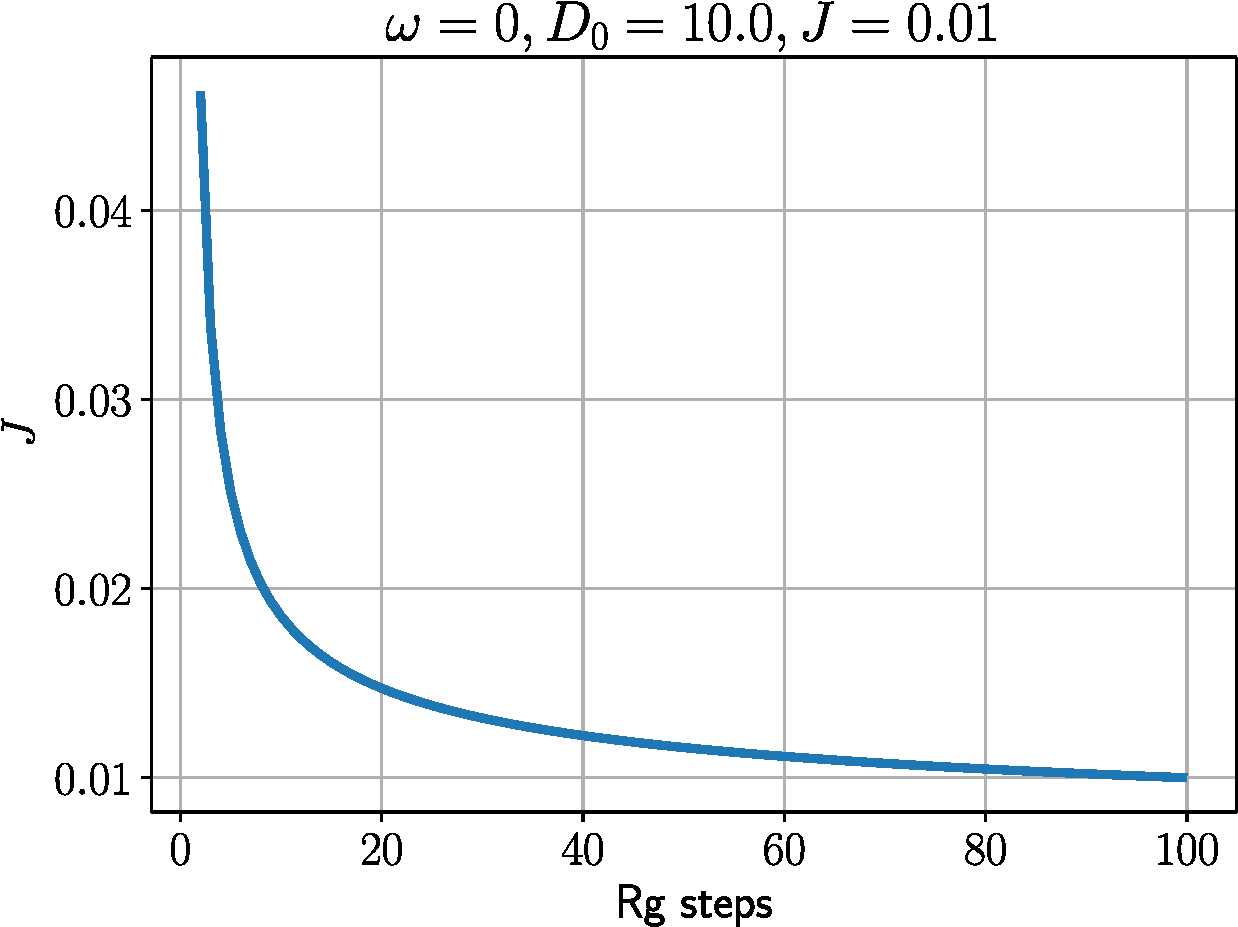
\includegraphics[width=0.45\textwidth]{../figures/relJ.pdf}
	\hspace*{\fill}
	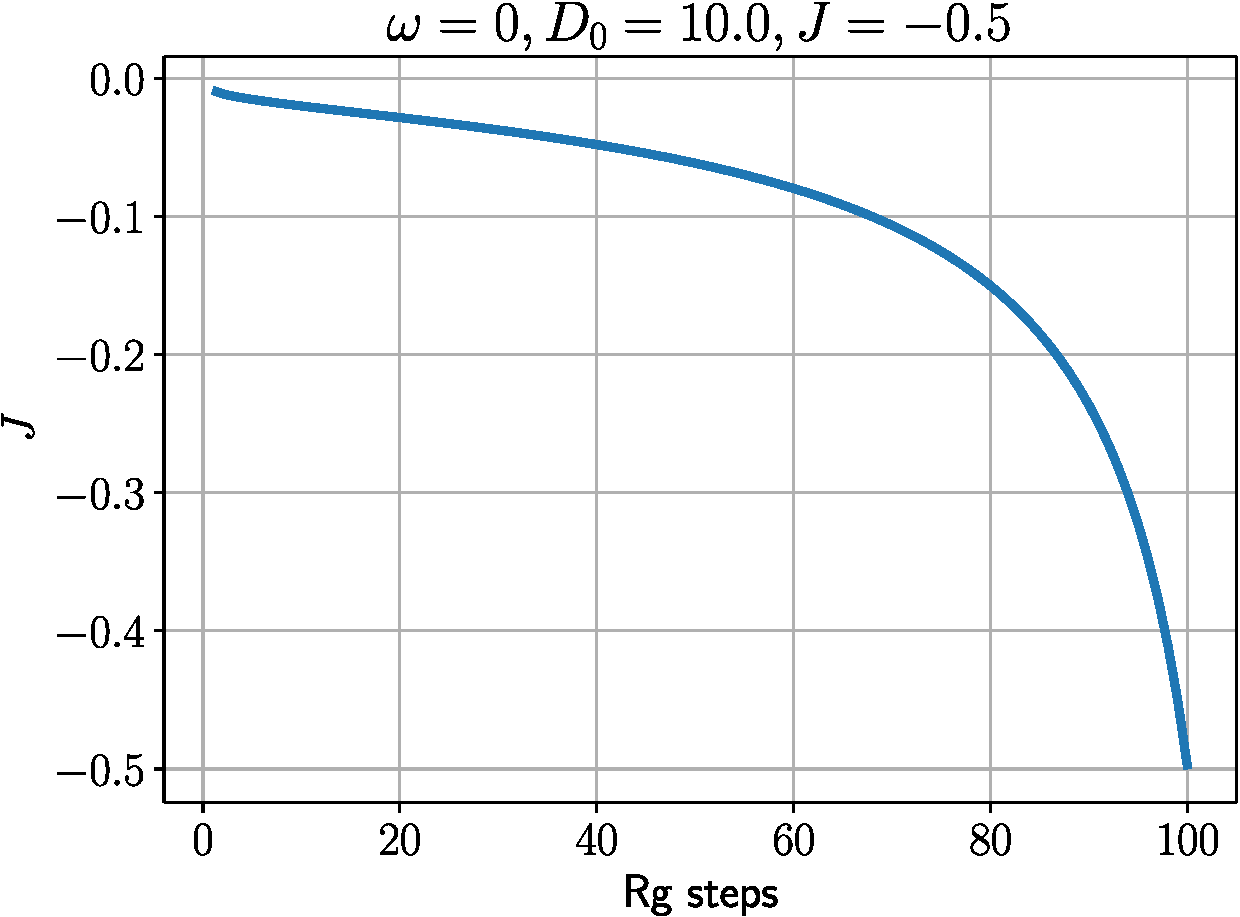
\includegraphics[width=0.45\textwidth]{../figures/rel2J.pdf}
	\captionof{figure}{Flow of \(J\) towards the strong-coupling fixed point (right) and the weak coupling saddle-point (left).  The x-axis indicates the index of the energy shell being decoupled. The largest value (UV) is the first step, and we go towards the left (IR).}
\end{center}
\begin{center}
	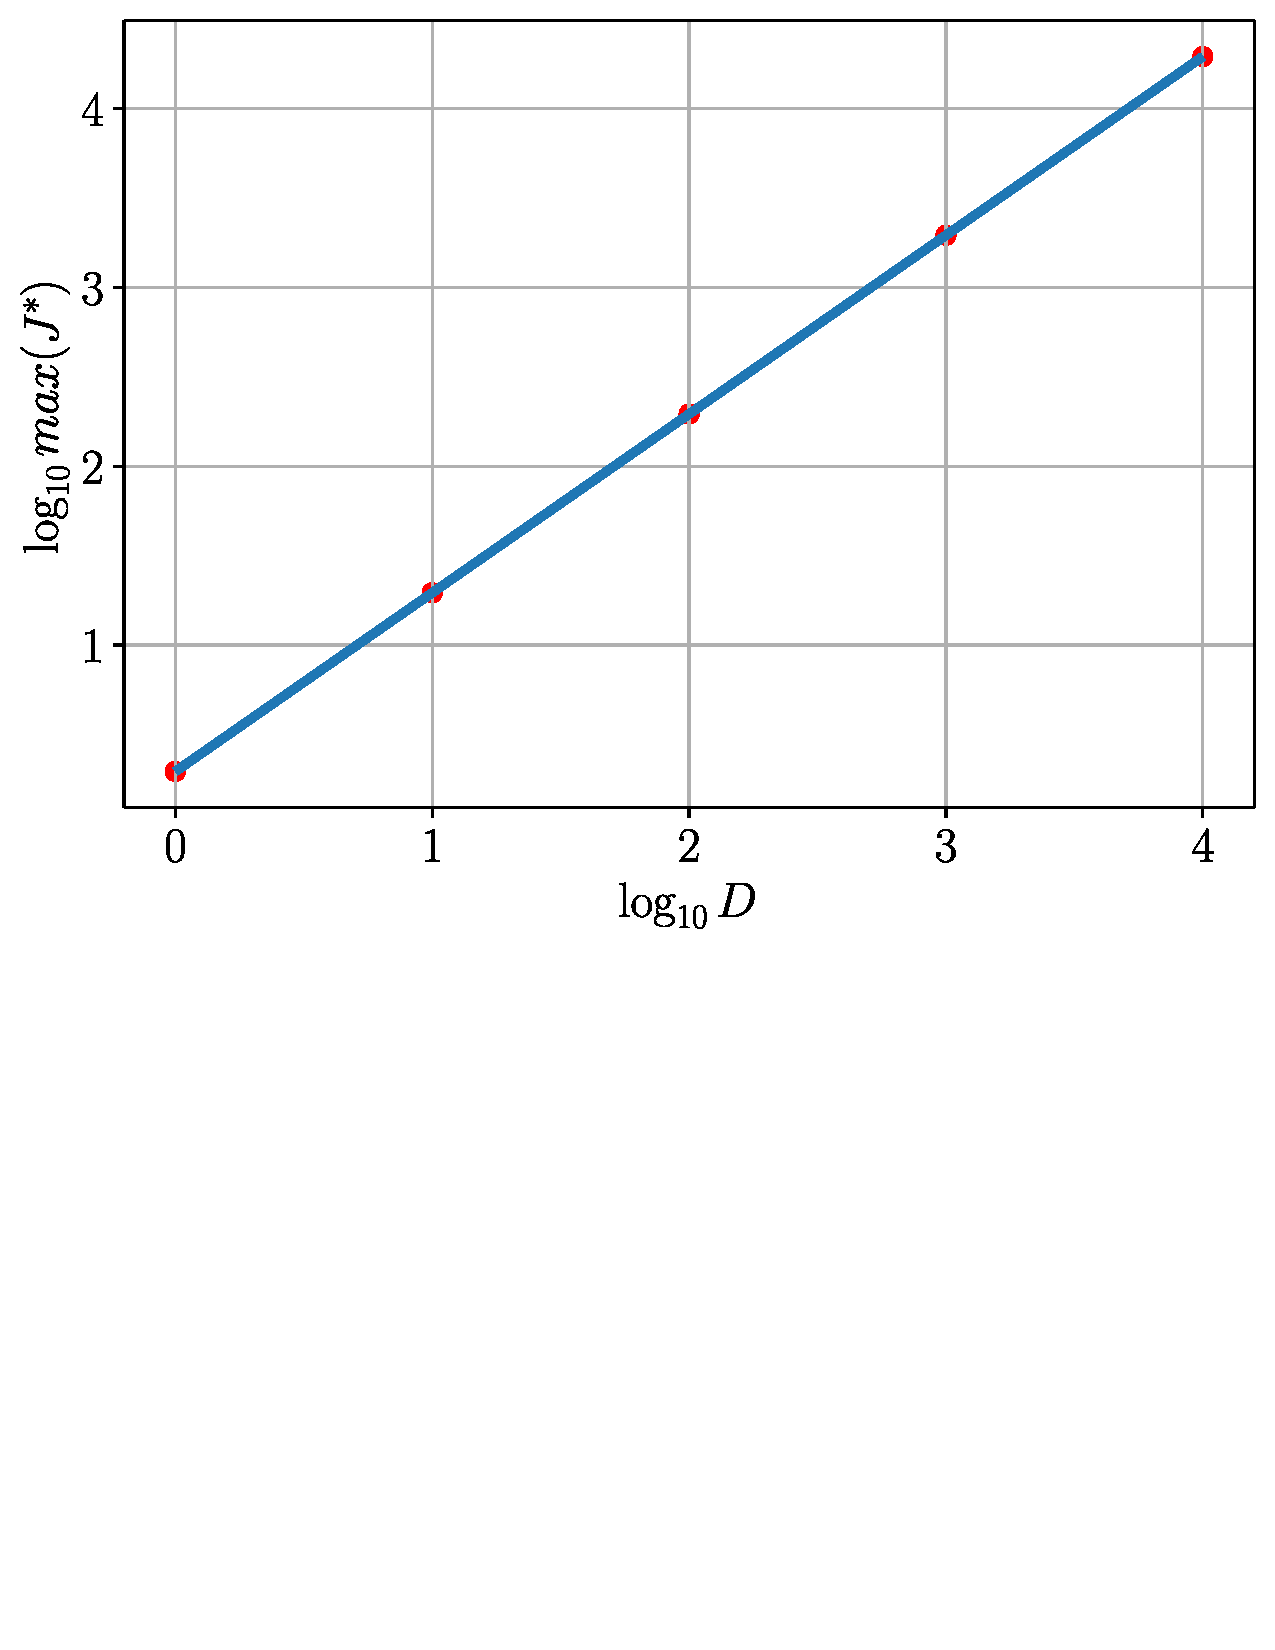
\includegraphics[scale=0.5]{../figures/JvsD_kondo.pdf}
	\captionof{figure}{Variation of the fixed point value \(J^*\) against the bare bandwidth, in log scale.}
	\label{JvsD-kondo}
\end{center}

\chapter{Connection between URG and Other Canonical Transformations}
\label{urg_canonical}
\section{Poor man's scaling (PMS)}
\subsection{Formalism}
We first describe the formalism of the poor man's scaling (PMS) method, first formulated by Anderson \cite{Anderson}. The problem is defined as
\begin{equation}\begin{aligned}
	\label{problem}
\mathcal{H}\ket{\Psi} = E\ket{\Psi}
\end{aligned}\end{equation}
\(\mathcal{H}\) is the total Hamiltonian and \(\ket{\Psi}\) and \(E\) are the exact eigenstate and eigenvalue of \(\mathcal{H}\). We imagine a separation of the total Hilbert space into two set of states, and we call these two states \(\ket{0}\) and \(\ket{1}\). This separation depends on which scattering term we want to kill by this transformation. For example, in the URG, we typically select a particular electron \(q\beta\) and then kill the  scattering terms that change the number of this state. In that case, \(\ket{0}\) will refer to the set of states \(\left\{\ket{\hat n_{q\beta}=0}\otimes\ket{\phi_0}\right\}\) and \(\ket{1}\) will refer to the set of states \(\left\{\ket{\hat n_{q\beta}=1}\otimes\ket{\phi_1}\right\}\). \(\ket{\phi_{0,1}}\) refer to the states of all the other electrons. As another example, if we wanted to separate the charge-Kondo and the spin-Kondo from the SIAM, we would want to kill the terms that scatter between the spin-full subspace \(\hat n_d=1\) to the spin-less subspace \(\hat{n_d}=0,2\). These two will then be the \(\ket{0}\) and \(\ket{1}\) sets. 
\\\\Keeping this separation in mind, the exact eigenstate \(\ket{\Psi}\) can be split as 
\begin{equation}\begin{aligned}
\ket{\Psi} = \sum_i \ket{\phi_0^i} + \sum \ket{\phi_1^i}
\end{aligned}\end{equation}
The Hamiltonian can also be split as 
\begin{equation}\begin{aligned}
\mathcal{H} = H_0 + V_+ + V_-
\end{aligned}\end{equation}
\(H_0\) does not scatter between \(\left\{\ket{0}\right\}\) and \(\left\{\ket{1}\right\}\). It contains the diagonal parts as well as scatterings inside the subspaces. \(V_\pm\) scatter between the subspaces:
\begin{equation}\begin{aligned}
V_+ \left\{\ket{0}\right\} \mapsto \left\{\ket{1}\right\},&& V_+ \ket{1} \to 0\\
V_- \left\{\ket{1}\right\} \mapsto \left\{\ket{0}\right\},&& V_- \ket{0} \to 0
\end{aligned}\end{equation}
The Schrodinger equation can thus be split into
\begin{equation}\begin{aligned}
H_0 \sum_i \ket{\phi^i_0} + V_-\sum_i \ket{\phi^i_1} &= E \sum_i \ket{\phi^i_0}\\
H_0 \sum_i \ket{\phi^i_1} + V_+\sum_i \ket{\phi^i_0} &= E \sum_i \ket{\phi^i_1}\\
\end{aligned}\end{equation}
Eliminating \(\sum_i \ket{\phi^i_1}\) gives
\begin{equation}\begin{aligned}
H_0 \sum_i \ket{\phi^i_0} + V_-\frac{1}{E_1 - H_0}V_+\sum_i \ket{\phi^i_0} &= E \sum_i \ket{\phi^i_0}\\
\end{aligned}\end{equation}
The effective Hamiltonian in this subspace is therefore
\begin{equation}\begin{aligned}
	\tilde{\mathcal{H}}_0 = H_0 + V_-\frac{1}{E - H_0}V_+
\end{aligned}\end{equation}
Similarly, eliminating \(\sum_i \ket{\phi^i_0}\) gives the effective Hamiltonian in the other subspace,
\begin{equation}\begin{aligned}
	\tilde{\mathcal{H}}_1 = H_0 + V_+\frac{1}{E - H_0}V_-
\end{aligned}\end{equation}
The total effective Hamiltonian that does not scatter between the two subspaces is
\begin{equation}\begin{aligned}
	\tilde{\mathcal{H}}(E) = H_0 + \underbrace{V_-\frac{1}{E - H_0}V_+ +  V_+\frac{1}{E - H_0}V_-}_\text{renormalization}
\end{aligned}\end{equation}
This is of course a function of whatever exact energy eigenvalue we chose, \(E\). Different choices will give different effective Hamiltonians. The renormalization will now be written in terms of the matrix elements. Since the entire \(\mathcal{H}_X\) must be Hermitian, we must have \(V_- = V_+^\dagger \equiv V\).
\begin{equation}\begin{aligned}
\Delta \mathcal{H}(E) = V\frac{1}{E - H_0}V^\dagger +  V^\dagger\frac{1}{E - H_0}V
\end{aligned}\end{equation}
Now take the first term and insert complete bases on both sides of \(V\) and \(V^\dagger\).
\begin{equation}\begin{aligned}
V\frac{1}{E - H_0}V^\dagger &= \sum_{ijk}\ket{\phi_0^i}\bra{\phi_0^i}V\ket{\phi_1^j}\bra{\phi_1^j}\frac{1}{E - H_0}\ket{\phi_1^j}\bra{\phi_1^j}V^\dagger\ket{\phi_0^k}\bra{\phi_0^k} \\
                &= \sum_{ijk}\ket{\phi_0^i}V_{ij}\bra{\phi_1^j}\frac{1}{E - H_0}\ket{\phi_1^j}V^\dagger_{kj}\bra{\phi_0^k}\\
\end{aligned}\end{equation}
where we defined \(\bra{\phi_0^i}V\ket{\phi_1^j} = V_{ij}\). We now approximate \(H_0\) by keeping just the diagonal part, and allowing the balance to redefine \(E\) into \(\omega\). Then, \(\left(E - H_0\right) \ket{\phi_{0,1}^j} \equiv \left(\omega_{0,1} - E_{0,1}^j\right) \ket{\phi_{0,1}^j}\). That gives
\begin{equation}\begin{aligned}
\label{pms_dropV}
V\frac{1}{E - H_0}V^\dagger &= \sum_{ijk}\ket{\phi_0^i}\bra{\phi_0^k}\frac{V_{ij}V^\dagger_{kj}}{\omega_1 - E^j_1}
\end{aligned}\end{equation}
The second term similarly gives
\begin{equation}\begin{aligned}
V^\dagger\frac{1}{E - H_0}V = \sum_{ijk}\ket{\phi_1^i}\bra{\phi_1^k}\frac{V^\dagger_{ji}V_{jk}}{\omega_0 - E^j_0}
\end{aligned}\end{equation}
The total renormalization becomes
\begin{equation}\begin{aligned}
	\Delta \mathcal{H}(E) = \sum_{ijk}\left(\frac{1}{\omega_1 - E^j_1}\ket{\phi_0^i}\bra{\phi_0^k}V_{ij}V^\dagger_{kj} + \frac{1}{\omega_0 - E^j_0}\ket{\phi_1^i}\bra{\phi_1^k}V^\dagger_{ji}V_{jk}\right)
\end{aligned}\end{equation}
This is a general expression that would work irrespective of whether you are decoupling multiple electrons or a single electron. However, the \(\omega\) are unknown and we need some prescription for replacing them. Since the \(E\) is the eigenstate of the initial state on which the scattering terms act, it makes sense to replace them with the initial state energy.
\begin{equation}\begin{aligned}
	\Delta \mathcal{H}(E) = \sum_{ijk}\left(\frac{1}{E_0^k - E^j_1}\ket{\phi_0^i}\bra{\phi_0^k}V_{ij}V^\dagger_{kj} + \frac{1}{E_1^k - E^j_0}\ket{\phi_1^i}\bra{\phi_1^k}V^\dagger_{ji}V_{jk}\right)
\end{aligned}\end{equation}
However, closer inspection reveals that this choice makes the renormalization non-Hermitian. So the correct choice is to keep both the initial and final energies.
\begin{equation}\begin{aligned}
	\Delta \mathcal{H} &= \frac{1}{2}\sum_{ijk}\frac{1}{\omega_1 - E^j_1}\left(\ket{\phi_0^i}\bra{\phi_0^k}V_{ij}V^\dagger_{kj} + \ket{\phi_0^k}\bra{\phi_0^i}V_{kj}V^\dagger_{ij}\right)\\
			   &+\frac{1}{2}\sum_{ijk}\frac{1}{\omega_0 - E^j_0}\left(\ket{\phi_1^i}\bra{\phi_1^k}V^\dagger_{ji}V_{jk} + \ket{\phi_1^k}\bra{\phi_1^i}V^\dagger_{jk}V_{ji}\right)\\
			   &= \frac{1}{2}\sum_{ijk}\left(\frac{1}{E_0^k - E^j_1}\ket{\phi_0^i}\bra{\phi_0^k}V_{ij}V^\dagger_{kj} + \frac{1}{E_0^k - E^j_1}\ket{\phi_0^k}\bra{\phi_0^i}V_{kj}V^\dagger_{ij}\right)\\
			   &+\frac{1}{2}\sum_{ijk}\left(\frac{1}{E_1^k - E^j_0}\ket{\phi_1^i}\bra{\phi_1^k}V^\dagger_{ji}V_{jk} + \frac{1}{E_1^k - E^j_0}\ket{\phi_1^k}\bra{\phi_1^i}V^\dagger_{jk}V_{ji}\right)
\end{aligned}\end{equation}
Therefore,
\begin{equation}\begin{aligned}
	\label{pmsren}
	\Delta \mathcal{H} &= \frac{1}{2}\sum_{ijk}\left(\frac{1}{E_0^k - E^j_1} + \frac{1}{E_0^i - E^j_1}\right)\ket{\phi_0^i}\bra{\phi_0^k}V_{ij}V^\dagger_{kj}\\
			   &+\frac{1}{2}\sum_{ijk}\left(\frac{1}{E_1^k - E^j_0}+ \frac{1}{E_1^i - E^j_0}\right)\ket{\phi_1^i}\bra{\phi_1^k}V^\dagger_{ji}V_{jk}\\
\end{aligned}\end{equation}
In summary, the prescription of replacing all \(\omega\) with the initial state energy will be correct only if the initial and final states are the same. This happens when we are decoupling a single-electron state - then the total renormalization is of the form \(c^\dagger T^\dagger c\) such that we start from an initial state, scatter to an intermediate state and then go back to the initial state so that the final state is the same as the initial state. However, if we are using PMS to decouple states in one-shot, each subspace will have multiple states and there might be terms where we do not end up at the initial state we started with. Then the correct prescription would be to use the mean of the initial and final state denominators.

One might wonder how we can generate higher order terms in this method. Eq.~\ref{pmsren}, as it stands, has only \(\mathcal{O}(V^2)\) terms. The higher order terms were actually dropped when we replaced \(H_0\) with its diagonal part in eq.~\ref{pms_dropV}. To see the higher order term, we do not drop the off-diagonal part in the denominator, but split the total \(H_0\) into a diagonal and an off-diagonal part: \(H_0 = H_d + X\). Note that \(X\) is off-diagonal in the subspace of the states that have not been decoupled yet but will be decoupled later. They represent scattering between the lower energy states. \(X\) is still diagonal with respect to the states that we \text{are} decoupling presently. The total effective Hamiltonian becomes
\begin{equation}\begin{aligned}
	\tilde{\mathcal{H}}(E) = H_0 + V\frac{1}{G_0(E)^{-1} - X}V^\dagger +  V^\dagger\frac{1}{G_0(E)^{-1} - X}V
\end{aligned}\end{equation}
where \(G_0(E)^{-1} = E - H_d\) is the inverse of the non-interacting Greens function. To allow computation, we can expand the denominator in powers of \(XG_0(E)^{-1}\):
\begin{equation}\begin{aligned}
	\label{pms_third}
	\Delta H \equiv \tilde{\mathcal{H}}(E) - H_0 =& VG_0(E)\left[1 + XG_0(E) + XG_0(E)XG_0(E) + ...\right] V^\dagger +  V^\dagger\frac{1}{G_0(E)^{-1} - X}V\\
	=& \underbrace{V G_0(E) V^\dagger + V^\dagger G_0(E) V}_\text{two vertex or one loop correction} + \underbrace{VG_0(E)XG_0(E)V^\dagger + V^\dagger G_0(E)XG_0(E)V}_\text{three vertex or two loop correction} \\
			       &+ \text{higher loop corrections}
\end{aligned}\end{equation}
\subsection{PMS third order equations for symmetric multi-channel Kondo model}
To get a clear idea of what the various terms in eq.~\ref{pms_third} mean, we will calculate the multi-channel Kondo model RG equations up to third order. The model is
\begin{equation}\begin{aligned}
	H = \sum_{k\sigma,\gamma}\epsilon_{k\sigma}^{(\gamma)}c^\dagger_{k\sigma}c^{(\gamma)}_{k\sigma} + \sum_{k\alpha,k^\prime \alpha^\prime,\gamma,a}J^a S_d^a \sigma^a_{\alpha\alpha^\prime}{c^{(\gamma)}_{k\alpha}}^\dagger c^{(\gamma)}_{k^\prime\alpha^\prime}
\end{aligned}\end{equation}
\(a\) goes over \(x,y,z\) and represents the directions. \(S_d^a\) therefore represents the spin operators for the impurity along the \(x,y\) and \(z\) directions. The labels \(k\alpha\) and \(k^\prime\alpha^\prime\) sum over the conduction electrons, while the index \(\gamma\) represents the channel. We will first calculate the second order terms. The virtual particle term is
\begin{equation}\begin{aligned}
	V G_0(E) V^\dagger = \sum_{k,k^\prime,\alpha,\alpha^\prime,q,\beta,\gamma,a,b}{c^{(\gamma)}_{q\beta}}^\dagger {c^{(\gamma)}_{k\alpha}} S_d^a \sigma^a_{\beta\alpha} \frac{J^a J^b}{E - H_d} {c^{(\gamma)}_{k^\prime\alpha^\prime}}^\dagger {c^{(\gamma)}_{q\beta}}S_d^b \sigma^b_{\alpha^\prime\beta}
\end{aligned}\end{equation}
The label \(q\) sums over the momentum states being decoupled \(\left( |\epsilon_q| \in \left[D-|\delta D|, D\right]  \right) \). The labels \(k,k^\prime\), on the other hand, sum over the momentum states that are not being decoupled, so they lie in the complimentary range. The denominator of the Greens function is the excitation energy \(\epsilon_q - \epsilon_{k^\prime}\). We will now simplify the term.
\begin{equation}\begin{aligned}
	V G_0(E) V^\dagger &= \sum_{k,k^\prime,\alpha,\alpha^\prime,q,\beta,\gamma, a,b} \frac{J^a J^b}{\epsilon_q - \epsilon_{k^\prime}}S_d^a \sigma^a_{\beta\alpha} S_d^b \sigma^b_{\alpha^\prime\beta}{c^{(\gamma)}_{q\beta}}^\dagger {c^{(\gamma)}_{k\alpha}} {c^{(\gamma)}_{k^\prime\alpha^\prime}}^\dagger {c^{(\gamma)}_{q\beta}}\\
			   &= \sum_{k,k^\prime,\alpha,\alpha^\prime,\beta,\gamma, a,b} \frac{J^a J^b}{\epsilon_q - \epsilon_{k^\prime}}S_d^a \sigma^a_{\beta\alpha} S_d^b \sigma^b_{\alpha^\prime\beta} {c^{(\gamma)}_{k\alpha}} {c^{(\gamma)}_{k^\prime\alpha^\prime}}^\dagger \sum_q {\hat n^{(\gamma)}_{q\beta}}\\
			   &= \sum_{k,k^\prime,\alpha,\alpha^\prime,\beta,\gamma, a,b} S_d^a \sigma^a_{\beta\alpha} S_d^b \sigma^b_{\alpha^\prime\beta} {c^{(\gamma)}_{k\alpha}} {c^{(\gamma)}_{k^\prime\alpha^\prime}}^\dagger \int_{-D}^{-D + |\delta D|} d\epsilon \rho(\epsilon) \frac{J^a J^b {\hat n^{(\gamma)}(\epsilon)_{\beta}}}{\epsilon_q - \epsilon_{k^\prime}}\\
			   &= \sum_{k,k^\prime,\alpha,\alpha^\prime,\beta,\gamma, a,b} S_d^a \sigma^a_{\beta\alpha} S_d^b \sigma^b_{\alpha^\prime\beta} {c^{(\gamma)}_{k\alpha}} {c^{(\gamma)}_{k^\prime\alpha^\prime}}^\dagger \frac{J^a J^b \rho(0) |\delta D|}{-D} ~~~\left[\hat n(\epsilon) = \theta(-\epsilon), |\epsilon_{k^\prime}| \ll D\right] \\
			   &= \sum_{\alpha,\alpha^\prime,a,b} S_d^a S_d^b \left(\sigma^b \sigma^a\right)_{\alpha^\prime,\alpha} \sum_{k,k^\prime,\gamma}{c^{(\gamma)}_{k\alpha}} {c^{(\gamma)}_{k^\prime\alpha^\prime}}^\dagger \frac{J^a J^b \rho(0) |\delta D|}{-D} \\
			   &= \sum_{\alpha,\alpha^\prime,a,b} \left(\frac{1}{4}\delta_{ab} + \frac{i}{2}\sum_c \epsilon^{abc}S_d^c\right) \left(\delta_{ab} + i\sum_c \epsilon^{bac}\sigma^c\right)_{\alpha^\prime,\alpha} \sum_{k,k^\prime,\gamma}{c^{(\gamma)}_{k\alpha}} {c^{(\gamma)}_{k^\prime\alpha^\prime}}^\dagger \frac{J^a J^b \rho(0) |\delta D|}{-D} \\
\end{aligned}\end{equation}
The spin part can now be simplified:
\begin{equation}\begin{aligned}
	\sum_{a,b} J^a J^b \left(\frac{1}{4}\delta_{ab} + \frac{i}{2}\sum_c \epsilon^{abc}S_d^c\right) \left(\delta_{ab} + i\sum_c \epsilon^{bac}\sigma^c\right)_{\alpha^\prime,\alpha} = \frac{\sum_a {J^a}^2}{4} \delta_{\alpha,\alpha^\prime} + \frac{1}{2}\sum_{a,b,c,c^\prime}J^a J^b \epsilon^{abc}\epsilon^{abc^\prime}S_d^c \left(\sigma^c\right)_{\alpha^\prime\alpha}\\
	= \frac{\sum_a {J^a}^2}{4} \delta_{\alpha,\alpha^\prime} + \frac{1}{2}\sum_c S_d^c \sigma^c_{\alpha^\prime\alpha}\left(\sum_{a,b,\atop{a\neq b}}J^a J^b - 2 J^c\sum_{a \atop{a \neq c}}J^a\right)
\end{aligned}\end{equation}
The constant part renormalizes a potential scattering, so we drop that part. The renormalization from the other part is
\begin{equation}\begin{aligned}
	\sum_{\alpha,\alpha^\prime,c} S_d^c \sigma^c_{\alpha^\prime\alpha} \sum_{k,k^\prime,\gamma}{c^{(\gamma)}_{k\alpha}} {c^{(\gamma)}_{k^\prime\alpha^\prime}}^\dagger \frac{\frac{1}{2}\left(\sum_{a,b,\atop{a\neq b}}J^a J^b - 2 J^c\sum_{a \atop{a \neq c}}J^a\right)\rho(0) |\delta D|}{-D}\\
	= \sum_{\alpha,\alpha^\prime,c} S_d^c \sigma^c_{\alpha^\prime\alpha} \sum_{k,k^\prime,\gamma}{c^{(\gamma)}_{k^\prime\alpha^\prime}}^\dagger {c^{(\gamma)}_{k\alpha}} \frac{\frac{1}{2}\left(\sum_{a,b,\atop{a\neq b}}J^a J^b - 2 J^c\sum_{a \atop{a \neq c}}J^a\right)\rho(0) |\delta D|}{D}
\end{aligned}\end{equation}
The virtual hole term \(V^\dagger G_0(E) V\) gives the same contribution. The total renormalization at second order is therefore
\begin{equation}\begin{aligned}
	\delta J^c = \frac{\left(\sum_{a,b,\atop{a\neq b}}J^a J^b - 2 J^c\sum_{a \atop{a \neq c}}J^a\right)\rho(0) |\delta D|}{D} = \frac{2J^{c+1}J^{c-1}\rho(0) |\delta D|}{D}
\end{aligned}\end{equation}
where \(\left\{c-1,c,c+1\right\}\) is a cyclic permutation of \(\left\{ x,y,z \right\} \). This reveals that the anisotropic Kondo coupling RG equations have a cyclic form:
\begin{equation}\begin{aligned}
	\delta J^x = \frac{2J^y J^z\rho(0) |\delta D|}{D}
\end{aligned}\end{equation}
Cyclic permutations of the labels \(x,y,z\) produce the other equations. From here on, we will assume \(J^a = J\) for simplicity. This gives, at second order,
\begin{equation}\begin{aligned}
	\delta J = \frac{2J^2\rho(0) |\delta D|}{D}
\end{aligned}\end{equation}

We now consider the third order term. The virtual hole three vertex term, \(V^\dagger G_0(E)XG_0(E)V\), is of the form
\begin{equation}\begin{aligned}
	J^3\sum_{q,k_1,k_2,k,k^\prime,\atop{\alpha,\alpha^\prime,\alpha_1,\alpha_2,\beta,\atop{\gamma_1,\gamma_2}}}{c^{(\gamma_1)}_{q\beta}}^\dagger {c^{(\gamma_1)}_{k\alpha}}\vec{S_d}\cdot\vec{\sigma}_{\beta \alpha} \frac{1}{E - H_d} {c^{(\gamma_2)}_{k_1 \alpha_1}}^\dagger c_{k_2 \alpha_2}^{(\gamma_2)}\vec{S_d}\cdot\vec{\sigma}_{\alpha_1 \alpha_2} \frac{1}{E - H_d} {c^{(\gamma_1)}_{k^\prime\alpha^\prime}}^\dagger {c^{(\gamma_1)}_{q\beta}}\vec{S_d}\cdot\vec{\sigma}_{\alpha^\prime \beta}
\end{aligned}\end{equation}
The other term among the two third order terms is the virtual particle term. The labels \(q,k,k^\prime,k_1,k_2\) run over the momentum states, \(\alpha,\alpha^\prime,\alpha_1,\alpha_2,\beta\) run over the spin indices and \(\gamma_1,\gamma_2\) run over the channel indices. \(q,\beta\) are the labels of the momentum states that are being decoupled. \(|\epsilon_q|\) therefore lies in the range \(\left[D, D - \delta D\right] \). The rest of the labels \((k,\alpha),(k_1,\alpha_1),(k_2,\alpha_2)\) lie in the compliment range and represent electrons that are not being decoupled at this step.

The denominator of the right-most Greens function measures the energy difference between the initial state and the state reached after the first excitation. This difference is \(\epsilon_q - \epsilon_{k^\prime}\). Similarly, the second Greens function has the energy difference between the initial state and the one obtained after two subsequent excitations. This difference is \(\epsilon_q - \epsilon_{k^\prime} + \epsilon_{k_2} - \epsilon_{k_1}\). With this substitution, we get 
\begin{equation}\begin{aligned}
	V^\dagger G_0(E)XG_0(E)V = J^3\sum_{q,k_1,k_2,k,k^\prime,\atop{\alpha,\alpha^\prime,\alpha_1,\alpha_2,\beta,\atop{\gamma_1,\gamma_2}}}\frac{{c^{(\gamma_1)}_{q\beta}}^\dagger {c^{(\gamma_1)}_{k\alpha}}\vec{S_d}\cdot\vec{\sigma}_{\beta \alpha} {c^{(\gamma_2)}_{k_1 \alpha_1}}^\dagger{c^{(\gamma_2)}_{k_2 \alpha_2}}\vec{S_d}\cdot\vec{\sigma}_{\alpha_1 \alpha_2} {c^{(\gamma_1)}_{k^\prime\alpha^\prime}}^\dagger {c^{(\gamma_1)}_{q\beta}}\vec{S_d}\cdot\vec{\sigma}_{\alpha \beta}}{\left(\epsilon_q - \epsilon_{k^\prime} + \epsilon_{k_2} - \epsilon_{k_1}\right)\left(\epsilon_q - \epsilon_{k^\prime}\right)}
\end{aligned}\end{equation}
The sum over \(q\) can be performed in the usual manner.
\begin{equation}\begin{aligned}
	\sum_q \frac{c^\dagger_{q\beta}c_{q\beta}}{\left(\epsilon_q - \epsilon_{k^\prime} + \epsilon_{k_2} - \epsilon_{k_1}\right)\left(\epsilon_q - \epsilon_{k^\prime}\right)} = \int_{-D}^{-D + |\delta D|} \frac{d\epsilon \rho(\epsilon)\hat n(\epsilon)}{\left(\epsilon - \epsilon_{k^\prime} + \epsilon_{k_2} - \epsilon_{k_1}\right)\left(\epsilon - \epsilon_{k^\prime}\right) }\\
	= \frac{\rho(0) |\delta D|}{\left(D + \epsilon_{k^\prime} - \epsilon_{k_2} + \epsilon_{k_1}\right)\left(D + \epsilon_{k^\prime}\right)}
\end{aligned}\end{equation}
where we have taken \(\rho(\epsilon) = \rho(0)\), \(\hat n(\epsilon) = \theta(-\epsilon)\) and \(\epsilon_q \simeq -D\). 

For the next step, note that \(\vec{S_d}\cdot\vec{\sigma}_{x,y} = \sum_{a}S_d^a \sigma^a_{x,y}\). Substituting this into \(V^\dagger G_0(E)XG_0(E)V\) gives
\begin{equation}\begin{aligned}
	&\sum_{\gamma_1,\gamma_2}\sum_{k_1,k_2,k,k^\prime}\sum_{\alpha,\alpha^\prime,\alpha_1,\alpha_2,\beta} \sum_{a,b,c}\frac{J^3\rho(0) |\delta D|}{\left(D + \epsilon_{k^\prime} - \epsilon_{k_2} + \epsilon_{k_1}\right)\left(D + \epsilon_{k^\prime}\right)} S_d^a\sigma^a_{\beta \alpha}S_d^b\sigma^b_{\alpha_1 \alpha_2}S_d^c \sigma^c_{\alpha^\prime \beta} c^{(\gamma_1)}_{k\alpha}{c^{(\gamma_2)}_{k_1 \alpha_1}}^\dagger c^{(\gamma_2)}_{k_2 \alpha_2} {c^{(\gamma_1)}_{k^\prime\alpha^\prime}}^\dagger
\end{aligned}\end{equation}
Now, note that all not all combinations of the momenta will renormalize the \(\vec{S_d}\cdot\vec{s}\) term of the Hamiltonian. In order for such a term to come out, the four remaining momenta must be contracted to two. The first set of terms that satisfy this requirement is given by the condition  \(k^\prime\alpha^\prime = k\alpha\). The renormalization from this subset of terms is
\begin{equation}\begin{aligned}
&\sum_{\gamma_1,\gamma_2}\sum_{k_1,k_2,k}\sum_{\alpha,\alpha_1,\alpha_2,\beta} \sum_{a,b,c}\frac{J^3\rho(0) |\delta D|}{\left(D + \epsilon_k - \epsilon_{k_2} + \epsilon_{k_1}\right)\left(D + \epsilon_k\right)} S_d^a\sigma^a_{\beta \alpha}S_d^b\sigma^b_{\alpha_1 \alpha_2}S_d^c \sigma^c_{\alpha \beta} {c^{(\gamma_2)}_{k_1 \alpha_1}}^\dagger c^{(\gamma_2)}_{k_2 \alpha_2}c^{(\gamma_1)}_{k\alpha}{c^{(\gamma_1)}_{k\alpha}}^\dagger \\
&=\sum_{\gamma_2}\sum_{k_1,k_2}\sum_{\alpha,\alpha_1,\alpha_2,\beta} \sum_{a,b,c} J^3\rho(0) |\delta D| S_d^a\sigma^a_{\beta \alpha}S_d^b\sigma^b_{\alpha_1 \alpha_2}S_d^c\sigma^c_{\alpha \beta}{c^{(\gamma_2)}_{k_1 \alpha_1}}^\dagger c^{(\gamma_2)}_{k_2 \alpha_2} \sum_{\gamma_1}\int_{0}^{D - |\delta D|}\frac{ d\epsilon\rho(\epsilon) }{\left(D + \epsilon - \epsilon_{k_2} + \epsilon_{k_1}\right)\left(D + \epsilon\right)}\\
&\simeq\sum_{\gamma_2}\sum_{k_1,k_2}\sum_{\alpha,\alpha_1,\alpha_2,\beta} \sum_{a,b,c} J^3\rho(0) |\delta D| S_d^a\sigma^a_{\beta \alpha}S_d^b\sigma^b_{\alpha_1 \alpha_2}S_d^c\sigma^c_{\alpha \beta}{c^{(\gamma_2)}_{k_1 \alpha_1}}^\dagger c^{(\gamma_2)}_{k_2 \alpha_2} \sum_{\gamma_1}\int_{0}^{D - |\delta D|}\frac{ d\epsilon\rho(\epsilon) }{\left(D + \epsilon\right)^2}\\
&=\frac{K \rho^2(0) J^3|\delta D|}{2D} \sum_{\alpha,\beta} \sum_{a,c,b}\sum_{\alpha_1,\alpha_2}S_d^a S_d^b S_d^c\sigma^a_{\beta \alpha} \sigma^b_{\alpha_1 \alpha_2} \sigma^c_{\alpha \beta} \sum_{k_1,k_2,\gamma_2}{c^{(\gamma_2)}_{k_1 \alpha_1}}^\dagger c^{(\gamma_2)}_{k_2 \alpha_2}~.\\
\end{aligned}\end{equation}
\(K = \sum_{\gamma_1}\) is the total number of channels. The other set of terms is given by the condition \(k_1\alpha_1 = k_2\alpha_2\). The renormalization from these terms can be calculated similarly:
\begin{equation}\begin{aligned}
	&\sum_{\gamma_1,\gamma_2}\sum_{k_1,k,k^\prime}\sum_{\alpha,\alpha^\prime,\alpha_1,\beta} \sum_{a,b,c}\frac{J^3 \rho(0) |\delta D|}{\left(D + \epsilon_{k^\prime}\right)^2} S_d^a\sigma^a_{\beta \alpha}S_d^b\sigma^b_{\alpha_1 \alpha_1}S_d^c \sigma^c_{\alpha^\prime \beta} c^{(\gamma_1)}_{k\alpha}{c^{(\gamma_2)}_{k_1 \alpha_1}}^\dagger c^{(\gamma_2)}_{k_1 \alpha_1} {c^{(\gamma_1)}_{k^\prime\alpha^\prime}}^\dagger\\
	&=\sum_{\gamma_1}\sum_{k,k^\prime}\sum_{\alpha,\alpha^\prime,\beta} \sum_{a,b,c}\frac{J^3 \rho(0) |\delta D|}{\left(D + \epsilon_{k^\prime}\right)^2} S_d^a\sigma^a_{\beta \alpha}S_d^b \mathrm{Trace}\left(\sigma^b\right)S_d^c \sigma^c_{\alpha^\prime \beta} c^{(\gamma_1)}_{k\alpha} \sum_{\gamma_2}\left[\int_{-D + |\delta D|}^0 d\epsilon \rho(\epsilon)\right] {c^{(\gamma_1)}_{k^\prime\alpha^\prime}}^\dagger\\
	&=0
\end{aligned}\end{equation}
The spin products can be simplified using the identity 
\begin{equation}\begin{aligned}
	\sum_{\alpha\beta}\sigma^a_{\beta \alpha} \sigma^c_{\alpha \beta} = \text{Trace}\left[\sigma^a \sigma^c\right] = 2\delta_{ac}~.
\end{aligned}\end{equation}
Using this identity, we get
\begin{equation}\begin{aligned}
	V^\dagger G_0(E)XG_0(E)V &=\frac{K \rho^2(0) J^3 |\delta D|}{D} \sum_{a,b}\sum_{\alpha_1,\alpha_2}S_d^a S_d^b S_d^a \sigma^b_{\alpha_1 \alpha_2} \sum_{k_1,k_2,\gamma_2}{c^{(\gamma_2)}_{k_1 \alpha_1}}^\dagger c^{(\gamma_2)}_{k_2 \alpha_2}\\
\end{aligned}\end{equation}
The products of the impurity spin operators can now be simplified:
\begin{equation}\begin{aligned}
	\sum_a S_d^a S_d^b S_d^a = \sum_a \left[S_d^b S_d^a + i\sum_c \epsilon^{abc}S_d^c\right] S_d^a = \frac{3}{4}S_d^b + i\sum_{a,c}  \epsilon^{abc}S_d^c S_d^a = \frac{3}{4}S_d^b + \frac{1}{2}i^2\sum_{a,c,e}  \epsilon^{abc}  \epsilon^{aec}S_d^e = -\frac{1}{4}S_d^b
\end{aligned}\end{equation}
Substituting this result in the renormalization gives
\begin{equation}\begin{aligned}
	V^\dagger G_0(E)XG_0(E)V &= -\frac{K\rho(0)^2 J^3 |\delta D|}{4D} \sum_{k_1,k_2,\alpha_1,\alpha_2,b,\gamma_2}S_d^b\sigma^b_{\alpha_1 \alpha_2}{c^{(\gamma_2)}_{k_1 \alpha_1}}^\dagger c^{(\gamma_2)}_{k_2 \alpha_2}\\
			    &= -\frac{K\rho(0)^2 J^3 |\delta D|}{4D} \sum_{k_1\alpha_1,k_2 \alpha_2,\gamma_2}\vec{S_d}\cdot\vec{\sigma}_{\alpha_1\alpha_2}{c^{(\gamma_2)}_{k_1 \alpha_1}}^\dagger c^{(\gamma_2)}_{k_2 \alpha_2}
\end{aligned}\end{equation}
The other term (virtual particle term) gives an equal contribution. The total renormalization is
\begin{equation}\begin{aligned}
	\delta J = \frac{2J^2 \rho(0) |\delta D|}{D}\left(1 - \frac{K\rho(0) J}{4}\right)
\end{aligned}\end{equation}


\subsection{PMS in the language of the URG - obtaining the \(\eta\) operators}
To make a better connection with URG, we next show how the PMS formalism works out for a single-electron decoupling. The corresponding problem can be phrased in the following manner. We want to decouple one electron at momentum \(q\) from the full Hamiltonian. We can split the exact wavefunction as
\begin{equation}\begin{aligned}
	\label{wf}
\ket{\Psi} = \ket{\Psi_0} + \ket{\Psi_1}
\end{aligned}\end{equation}
where \(\ket{\Psi_0} = \left(1 - \hat n_{q}\right)\ket{\Psi^N}\) is that part of the wavefunction where the state \(q\) is occupied. \(\ket{\Psi^N_1} = \hat n_q \ket{\Psi}\) is that part of the wavefunction where the state \(q\) is occupied. We can also split the Hamiltonian as
\begin{equation}\begin{aligned}
	\label{hami}
\mathcal{H} = \mathcal{H}^d + V_0 + V_+ + V_-
\end{aligned}\end{equation}
\(\mathcal{H}^d\) is the diagonal part; it has the purely energy terms as well as self-energies that may arise from the diagonal parts of interactions; \(V_0\) is the purely off-diagonal term that does not change \(\hat n_q\); it is the scattering \textit{inside} the low energy subspace. \(V_+\) and \(V_-\) are the purely off-diagonal terms that \textit{do} change \(\hat n_q\); \(V_+\) takes you from \(\hat n_q = 0\) to \(\hat n_q = 1\) and \(V_-\) does the opposite.
\\\\Substituting eqs.~\ref{hami} and \ref{wf} in eq.~\ref{problem} gives
\begin{equation}\begin{aligned}
	\left(\mathcal{H}^d + V_0 + V_+ + V_-\right)\left(\ket{\Psi_0} + \ket{\Psi_1}\right) = E\left(\ket{\Psi_0} + \ket{\Psi_1}\right)
\end{aligned}\end{equation}
Gathering the kets with \(\hat n_q = 0,1\) gives
\begin{equation}\begin{aligned}
	\left(\mathcal{H}^d_0 + V_0\right)\ket{\Psi_0} + V_- \ket{\Psi_1} = E\ket{\Psi_0}\\
	\left(\mathcal{H}^d_1 + V_0\right)\ket{\Psi_1} + V_+\ket{\Psi_0} = E\ket{\Psi_1}
\end{aligned}\end{equation}
The second equation can be written as
\begin{equation}\begin{aligned}
\ket{\Psi_1} = \eta^\dagger \ket{\Psi_0}
\end{aligned}\end{equation}
where
\begin{equation}\begin{aligned}
	\left(\eta^\dagger\right)_\text{PMS} = \frac{1}{E - \mathcal{H}^d_1 - V_0}V_+
\end{aligned}\end{equation}
Substituting this in the first equation gives
\begin{equation}\begin{aligned}
	\label{reneq}
	\left(\mathcal{H}^d_0 + V_0 + V_- \eta^\dagger\right)\ket{\Psi_0} = E\ket{\Psi_0}
\end{aligned}\end{equation}
This new Hamiltonian,
\begin{equation}\begin{aligned}
	\tilde{\mathcal{H}}_0 = \mathcal{H}^d_0 + V_0 + V_- \eta^\dagger
\end{aligned}\end{equation}
has the high energy mode removed; the scattering terms start from the low energy subspace and end at the low energy subspace as well. The renormalization in the low energy subspace scatterings  is
\begin{equation}\begin{aligned}
	\label{deltaV}
\Delta V_0 = V_- \eta^\dagger
\end{aligned}\end{equation}
If we eliminate \(\ket{\Psi_0}\) instead of \(\ket{\Psi_1}\), we get the renormalized equation in the high energy subspace:
\begin{equation}\begin{aligned}
\ket{\Psi_0} = \eta \ket{\Psi_1}
\end{aligned}\end{equation}
where
\begin{equation}\begin{aligned}
	\left(\eta\right)_\text{PMS} = \frac{1}{E - \mathcal{H}^d_0 - V_0}V_-
\end{aligned}\end{equation}
,so
\begin{equation}\begin{aligned}
	\left(\mathcal{H}^d_1 + V_0 + V_+ \eta\right)\ket{\Psi_1} = E\ket{\Psi_1}
\end{aligned}\end{equation}
The renormalized Hamiltonian in the high energy subspace is thus
\begin{equation}\begin{aligned}
	\tilde{\mathcal{H}}_1 = \mathcal{H}^d_1 + V_0 + V_+ \eta
\end{aligned}\end{equation}
If we want to keep both the high energy and low energy parts of the Hamiltonian, the new Hamiltonian is
\begin{equation}\begin{aligned}
	\label{transham}
	\tilde{\mathcal{H}} &= \tilde{\mathcal{H}}_1 \hat n + \tilde{\mathcal{H}}_0 \left(1 - \hat n\right)\\
&= \mathcal{H}^d_0 + \mathcal{H}^d_1 + V_0 + V_+ \eta + V_- \eta^\dagger
\end{aligned}\end{equation}
The total renormalization is
\begin{equation}\begin{aligned}
	\left(\Delta \mathcal{H}\right)_\text{PMS} = V_+ \left(\eta\right)_\text{PMS} + V_- \left(\eta^\dagger\right)_\text{PMS}
\end{aligned}\end{equation}
It can be shown that if we define a unitary operator \(U = 1 - \eta + \eta^\dagger\), the transformed Hamiltonian \(U \mathcal{H} U^\dagger\) is the same as eq.~\ref{transham}. This, along with the properties of \(\eta\), have been shown in section \ref{urgform}. The important feature of eq.~\ref{transham} is that there is no term in the transformed Hamiltonian which scatters between \(\ket{\Psi_0}\) and \(\ket{\Psi_0}\)- the two subspaces have been truly decoupled.
\begin{equation}\begin{aligned}
	\left[U \mathcal{H} U^\dagger, n_q\right] = 0
\end{aligned}\end{equation}
We can write down the renormalized Schrodinger equation in the low energy subspace, from eq.~\ref{reneq},
\begin{equation}\begin{aligned}
	\tilde{\mathcal{H}}_0 \ket{\Psi_0} = E\ket{\Psi_0}
\end{aligned}\end{equation}
and again repeat the entire process. \(\tilde{\mathcal{H}}_0\) now takes the place of \(\mathcal{H}\) and \(\ket{\Psi_0}\) takes the place of \(\ket{\Psi}\) in eq.~\ref{problem}.
\\\\The expression for URG is obtained in an almost identical way. The only difference is that instead of starting with the exact eigenpair (\(E,\ket{\Psi}\)), we start with a more general pair (\(\tilde{\mathcal{H}}, \ket{\Phi}\)) where \(\ket{\Phi}\) is not necessarily an exact eigenstate of \(\mathcal{H}\). It is defined by \(\mathcal{H}^\prime\), which is in turn defined as \(\hat n_q \mathcal{H}^\prime\left(1 - \hat n_q\right) = 0\). \(\ket{\Phi}\) is then defined by
\begin{equation}\begin{aligned}
\mathcal{H}\ket{\Phi} = \mathcal{H}^\prime \ket{\Phi}
\end{aligned}\end{equation}
This definition of \(\mathcal{H}^\prime\) is the very minimum that we must have in order to fulfill our goal (decouple \(q\)). 
\\\\The operators \(\eta\) and its conjugate change accordingly:
\begin{equation}\begin{aligned}
	\left(\eta\right)_\text{URG} &= \frac{1}{\tilde{\mathcal{H}} - \mathcal{H}^d_0 - V_0}V_-\\
     &= \frac{1}{\hat \omega - \mathcal{H}^d_0}V_-\\
\end{aligned}\end{equation}
where \(\hat \omega \equiv \mathcal{H}^\prime - V_0\) now embodies the quantum fluctuations inherent in the Hamiltonian through the scattering term \(V_0\). Similarly,
\begin{equation}\begin{aligned}
	\left(\eta^\dagger\right)_\text{URG} &= \frac{1}{\hat \omega - \mathcal{H}^d_1}V_+\\
\end{aligned}\end{equation}
The renormalization is again
\begin{equation}\begin{aligned}
	\left(\Delta \mathcal{H}\right)_\text{URG} = V_+\left(\eta\right)_\text{URG} + V_-\left(\eta^\dagger\right)_\text{URG}
\end{aligned}\end{equation}
This again allows us to write down a unitary operator that decouples the entangled state:
\begin{equation}\begin{aligned}
	U =  1 - \eta + \eta^\dagger, \left[\hat n_q, U \mathcal{H} U^\dagger\right] = 0
\end{aligned}\end{equation}
where \(\tilde{\mathcal{H}} = U^\dagger \mathcal{H} U\). We can now write down a new problem in this decoupled space with the rotated items and attempt to decouple another electron \(q^\prime\). We will again choose some general eigenpair (\(\mathcal{H}^\prime,\ket{\Phi}\)) such that \(\tilde{\mathcal{H}}\ket{\Phi} = \mathcal{H}^{\prime}\ket{\Phi}\) and \(\left[\mathcal{H}^{\prime},\hat n_{q^\prime}\right]=0\).
\\\\Summarizing, the general Hamiltonian is not diagonal in the Fock space basis.
URG, in order to proceed, selects one non-Fock basis of states \(\ket{\Phi}\) such that \(q\) is decoupled in that Hamiltonian.
Since there can be lots of such basis, there is a freedom in this choice.
With this basis in mind, URG then finds a unitary operator which when operated on the Hamiltonian takes us to the form in which it is diagonal in the Fock space basis.
Note that this form is a function of the chosen \(\ket{\Phi}\).
We then select the second degree of freedom and repeat the process.
What PMS does is, it exploits the freedom of choice and selects the exact eigenstate \(\ket{\Psi}\) of the Hamiltonian as the non-Fock basis \(\ket{\Phi}\).
Doing that returns a rotated Hamiltonian which is diagonal in \(q\), and is a function of the chosen state, same as URG. The conclusion is that depending on which state we choose as our diagonal non-Fock basis, URG and PMS will cause flows along different lines in general.
\\\\As the couplings flow, \(V_0\) will also flow, leading to a flow of \(\hat\omega\). Just at the fixed point, the denominator of URG vanishes, giving the equation
\begin{equation}\begin{aligned}
	\left(\hat\omega - \mathcal{H}_1^d\right)V_+\ket{\Psi_0} \text{ or } \left(\hat\omega - \mathcal{H}_1^d\right)V_-\ket{\Psi_1}
\end{aligned}\end{equation}
This means that one of the eigenvalues of \(\hat\omega\) matches with the eigenvalue of the diagonal part \(\mathcal{H}^d\), either in the occupied sector (\(\mathcal{H}^d_1\)) or unoccupied sector (\(\mathcal{H}^d_1\)). Since the eigenvalues are unchanged during the unitary renormalization, this implies that \(\omega\) takes up one of the eigenvalues of the whole Hamiltonian \(\mathcal{H}\). This will correspond to the fixed point obtained from PMS if we had started PMS with that eigenvalue.
\\\\In short, while the PMS flow is parametrised by one of the exact energy eigenvalues \(E\), the URG flow is parametrised by a non-trivial operator \(\hat \omega\) which incorporates both a diagonal part and an off-diagonal part and itself flows under the URG. At the fixed point, the off-diagonal part cancels out and the \(\hat\omega\) finally flows to one of the energy eigenvalues and the URG fixed point matches with one of the PMS fixed points.
\begin{figure}
\centering
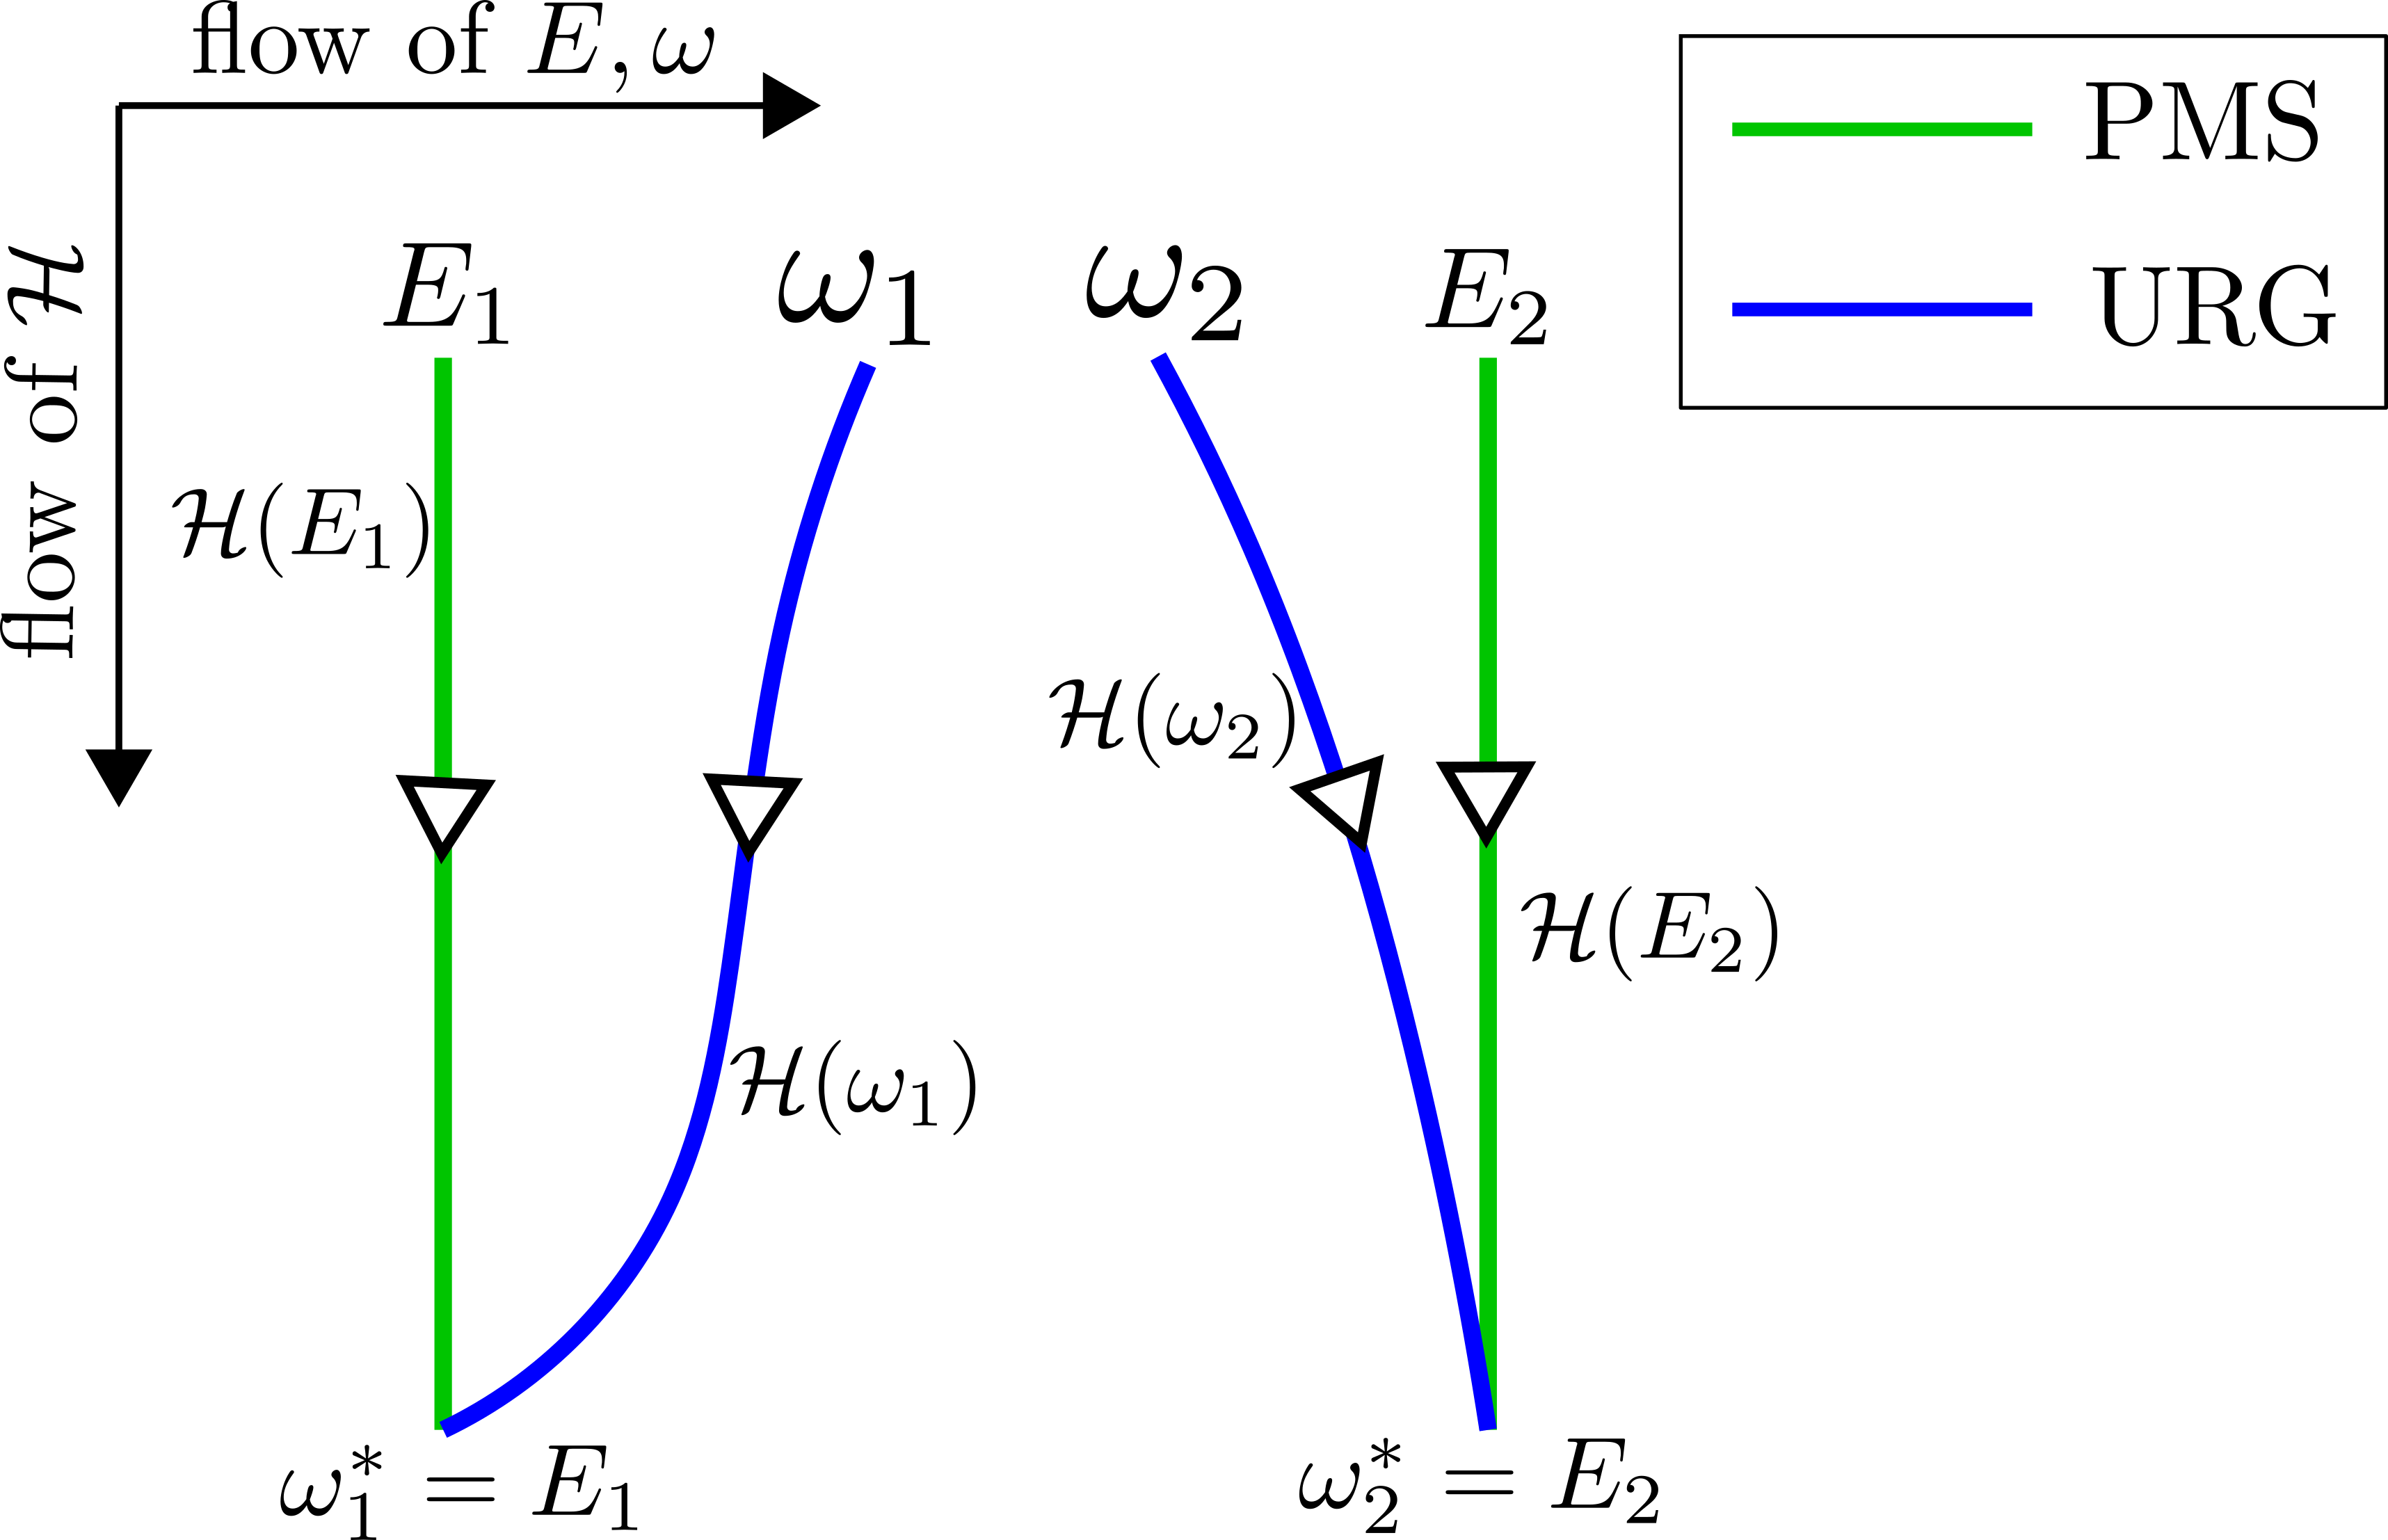
\includegraphics[width=0.6\textwidth]{pms_vs_urg.png}
\caption{Flows of PMS(green) and URG(blue)}
\end{figure}
\subsection{PMS for the single impurity Anderson model}
To demonstrate the implementation, we can look at a specific model. For the SIAM,
\begin{equation}\begin{aligned}
	\mathcal{H} = \sum_{k\sigma}\left(\epsilon_k \tau_{k\sigma} + V c^\dagger_{k\sigma}c_{d\sigma} + \text{h.c.}\right)
\end{aligned}\end{equation}
where \(\tau = \hat n - \frac{1}{2}\). We want to decouple the state \(q\beta\) from the rest of the electrons. We have \({H}_0 = \epsilon_d\hat n_d + U \hat n_{d\uparrow}n_{d\downarrow} + \sum_{k\sigma} \epsilon_k \hat n_{k\sigma}\), \(V_0 = \sum_{k<q,\sigma}c^\dagger_{k\sigma}c_{d\sigma}+\text{h.c.}\), \(V_+ = V c^\dagger_{q\beta}c_{d\beta}\) and \(V_- = V c^\dagger_{d\beta}c_{q\beta}\). The renormalization in particle sector
\begin{equation}\begin{aligned}
	\Delta V_0 &=  c^\dagger_{d\beta}c_{q\beta}\frac{1}{\left(E - V_0\right) - \hat{\mathcal{H}}^d_0}c^\dagger_{q\beta}c_{d\beta}\\
\end{aligned}\end{equation}
The intermediate energy (at the propagator) is
\begin{equation}\begin{aligned}
	\hat{\mathcal{H}}^d_0 = \sum_{k,\sigma}\epsilon_k \tau_{k\sigma} + \epsilon_d \hat n_{d\overline\beta}
\end{aligned}\end{equation}
This is because the \(c_{d\beta}\) at the right of the propagator ensures that we must have \(\hat n_{d\beta}=0\) at the propagator.
\begin{equation}\begin{aligned}
	\Delta V_0 &=  c^\dagger_{d\beta}c_{q\beta}\frac{1}{\left(E - V_0\right) - \sum_{k,\sigma}\epsilon_k \tau_{k\sigma} - \epsilon_d \hat n_{d\overline\beta}}c^\dagger_{q\beta}c_{d\beta}\\
\end{aligned}\end{equation}
Since \(E\) is the exact eigenvalue, we do not have an expression for it. Instead, we approximate \(E - V_0\) by substituting it with the current diagonal part corresponding to the initial state on which this entire term will act. The intial state is characterized by \(\hat n_{q\beta}=0\) and \(\hat n_{d\beta} = 1\), so
\begin{equation}\begin{aligned}
	E - V_0= \sum_{k<q,\sigma}\epsilon_k \tau_{k\sigma} - \frac{1}{2}\epsilon_q + \epsilon_d + \left(\epsilon_d + U\right)\hat n_{d\overline\beta}
\end{aligned}\end{equation}
The \(- \frac{1}{2}\epsilon_q\) comes from substituting \(\hat n_{q\beta}=0\) in \(\epsilon_q \tau_{q\beta}\).
\\\\ Substituting this in \(\Delta V_0\) gives
\begin{equation}\begin{aligned}
\Delta V_0 &=  c^\dagger_{d\beta}c_{q\beta}\frac{1}{-\frac{1}{2}\epsilon_q -\epsilon_q \tau_{q\beta} + \epsilon_d + U\hat n_{d\overline\beta}}c^\dagger_{q\beta}c_{d\beta}\\
&=  c^\dagger_{d\beta}c_{q\beta}\frac{1}{-\epsilon_q + \epsilon_d + U\hat n_{d\overline\beta}}c^\dagger_{q\beta}c_{d\beta}\\
&=  c^\dagger_{d\beta}c_{q\beta}c^\dagger_{q\beta}c_{d\beta}\frac{1}{-\epsilon_q + \epsilon_d + U\hat n_{d\overline\beta}}\\
&=  -c^\dagger_{d\beta}c_{q\beta}c^\dagger_{q\beta}c_{d\beta}\frac{1}{\epsilon_q - \epsilon_d - U\hat n_{d\overline\beta}}\\
&=  \left(1 - \hat n_{q\beta}\right)\left(\frac{-\hat n_{d\beta}\hat n_{d\overline\beta}}{\epsilon_q - \epsilon_d - U} + \frac{-\hat n_{d\beta}\left(1 - \hat n_{d\overline\beta}\right)}{\epsilon_q - \epsilon_d}\right)\\
\end{aligned}\end{equation}
On the second line, we substituted \(\tau_{q\beta} = \frac{1}{2}\) in the denominator, which is ensured by the \(c^\dagger_{q\beta}\) to the right of the propagator. The first term renormalizes the energy of the doublon state and the second term renormalizes that of the singly-occupied state:
\begin{equation}\begin{aligned}
\Delta E_2 &= \frac{-1}{\epsilon_q - \epsilon_d - U}\\
\Delta E_1 &= \frac{-1}{\epsilon_q - \epsilon_d}
\end{aligned}\end{equation}
The renormalization in the hole sector is
\begin{equation}\begin{aligned}
	\Delta V_0 &=  c^\dagger_{q\beta}c_{d\beta}\frac{1}{\left(E - V_0\right) - \hat {\mathcal{H}}^d_0}c^\dagger_{d\beta}c_{q\beta}\\
		   &=  c^\dagger_{q\beta}c_{d\beta}\frac{1}{\left(E - V_0\right) - \sum_{k,\sigma}\epsilon_k\tau_{k\sigma} - \epsilon_d - \left(\epsilon_d + U\right)\hat n_{d\overline\beta}}c^\dagger_{d\beta}c_{q\beta}
\end{aligned}\end{equation}
This time we substitute
\begin{equation}\begin{aligned}
E - V_0 &= \sum_{k<q,\sigma}\epsilon_k \tau_{k\sigma} + \tau_{q\beta} \epsilon^-_q + \epsilon_d\hat n_{d\overline\beta}\\
&= \sum_{k<q,\sigma}\epsilon_k \tau_{k\sigma} + \frac{1}{2} \epsilon^-_q + \epsilon_d\hat n_{d\overline\beta}\\
\end{aligned}\end{equation}
In the last step we put \(\tau_{q\beta}=\frac{1}{2}\) because the state is occupied in the initial configuratin. Note that since the electron \(q\beta\) was occupied in the intial state, the energy \(\epsilon^-_q\) in this sector must be opposite to that of the particle sector, \(\epsilon_q\). Hence \(\epsilon^-_q = -\epsilon_q\), which gives
\begin{equation}\begin{aligned}
\Delta V_0 & = c^\dagger_{q\beta}c_{d\beta}\frac{1}{-\frac{1}{2} \epsilon_q -\epsilon^-_q\tau_{q\beta} - \epsilon_d - U\hat n_{d\overline\beta}}c^\dagger_{d\beta}c_{q\beta}\\
& = c^\dagger_{q\beta}c_{d\beta}c^\dagger_{d\beta}c_{q\beta}\frac{1}{-\epsilon_q - \epsilon_d - U\hat n_{d\overline\beta}}\\
& = \hat n_{q\beta}\left(\frac{-\left(1 - \hat n_{d\beta}\right)\hat n_{d\overline\beta}}{\epsilon_q + \epsilon_d + U} + \frac{-\left(1 - \hat n_{d\beta}\right)\left(1 - \hat n_{d\overline\beta}\right)}{\epsilon_q + \epsilon_d}\right)\\
\end{aligned}\end{equation}
In the second line, we put \(\epsilon^-_q = -\epsilon_q\) and \(\tau_{q\beta} = -\frac{1}{2}\). The first term renormalizes the singly-occupied state while the second term renormalizes the holon state. Combining with the particle sector results, the total renormalization in all the three impurity states (holon, single and doublon) are
\begin{equation}\begin{aligned}
\Delta E_0 &= -\frac{1}{\epsilon_q + \epsilon_d}\\
\Delta E_1 &= -\frac{1}{\epsilon_q + \epsilon_d + U} - \frac{1}{\epsilon_q - \epsilon_d}\\
\Delta E_2 &= -\frac{1}{\epsilon_q - \epsilon_d - U}\\
\end{aligned}\end{equation}
These results are also obtained in ref.~\cite{hewson}. The complete process is depicted in fig.~\ref{pmsflow}.
\begin{figure}
    \centering
    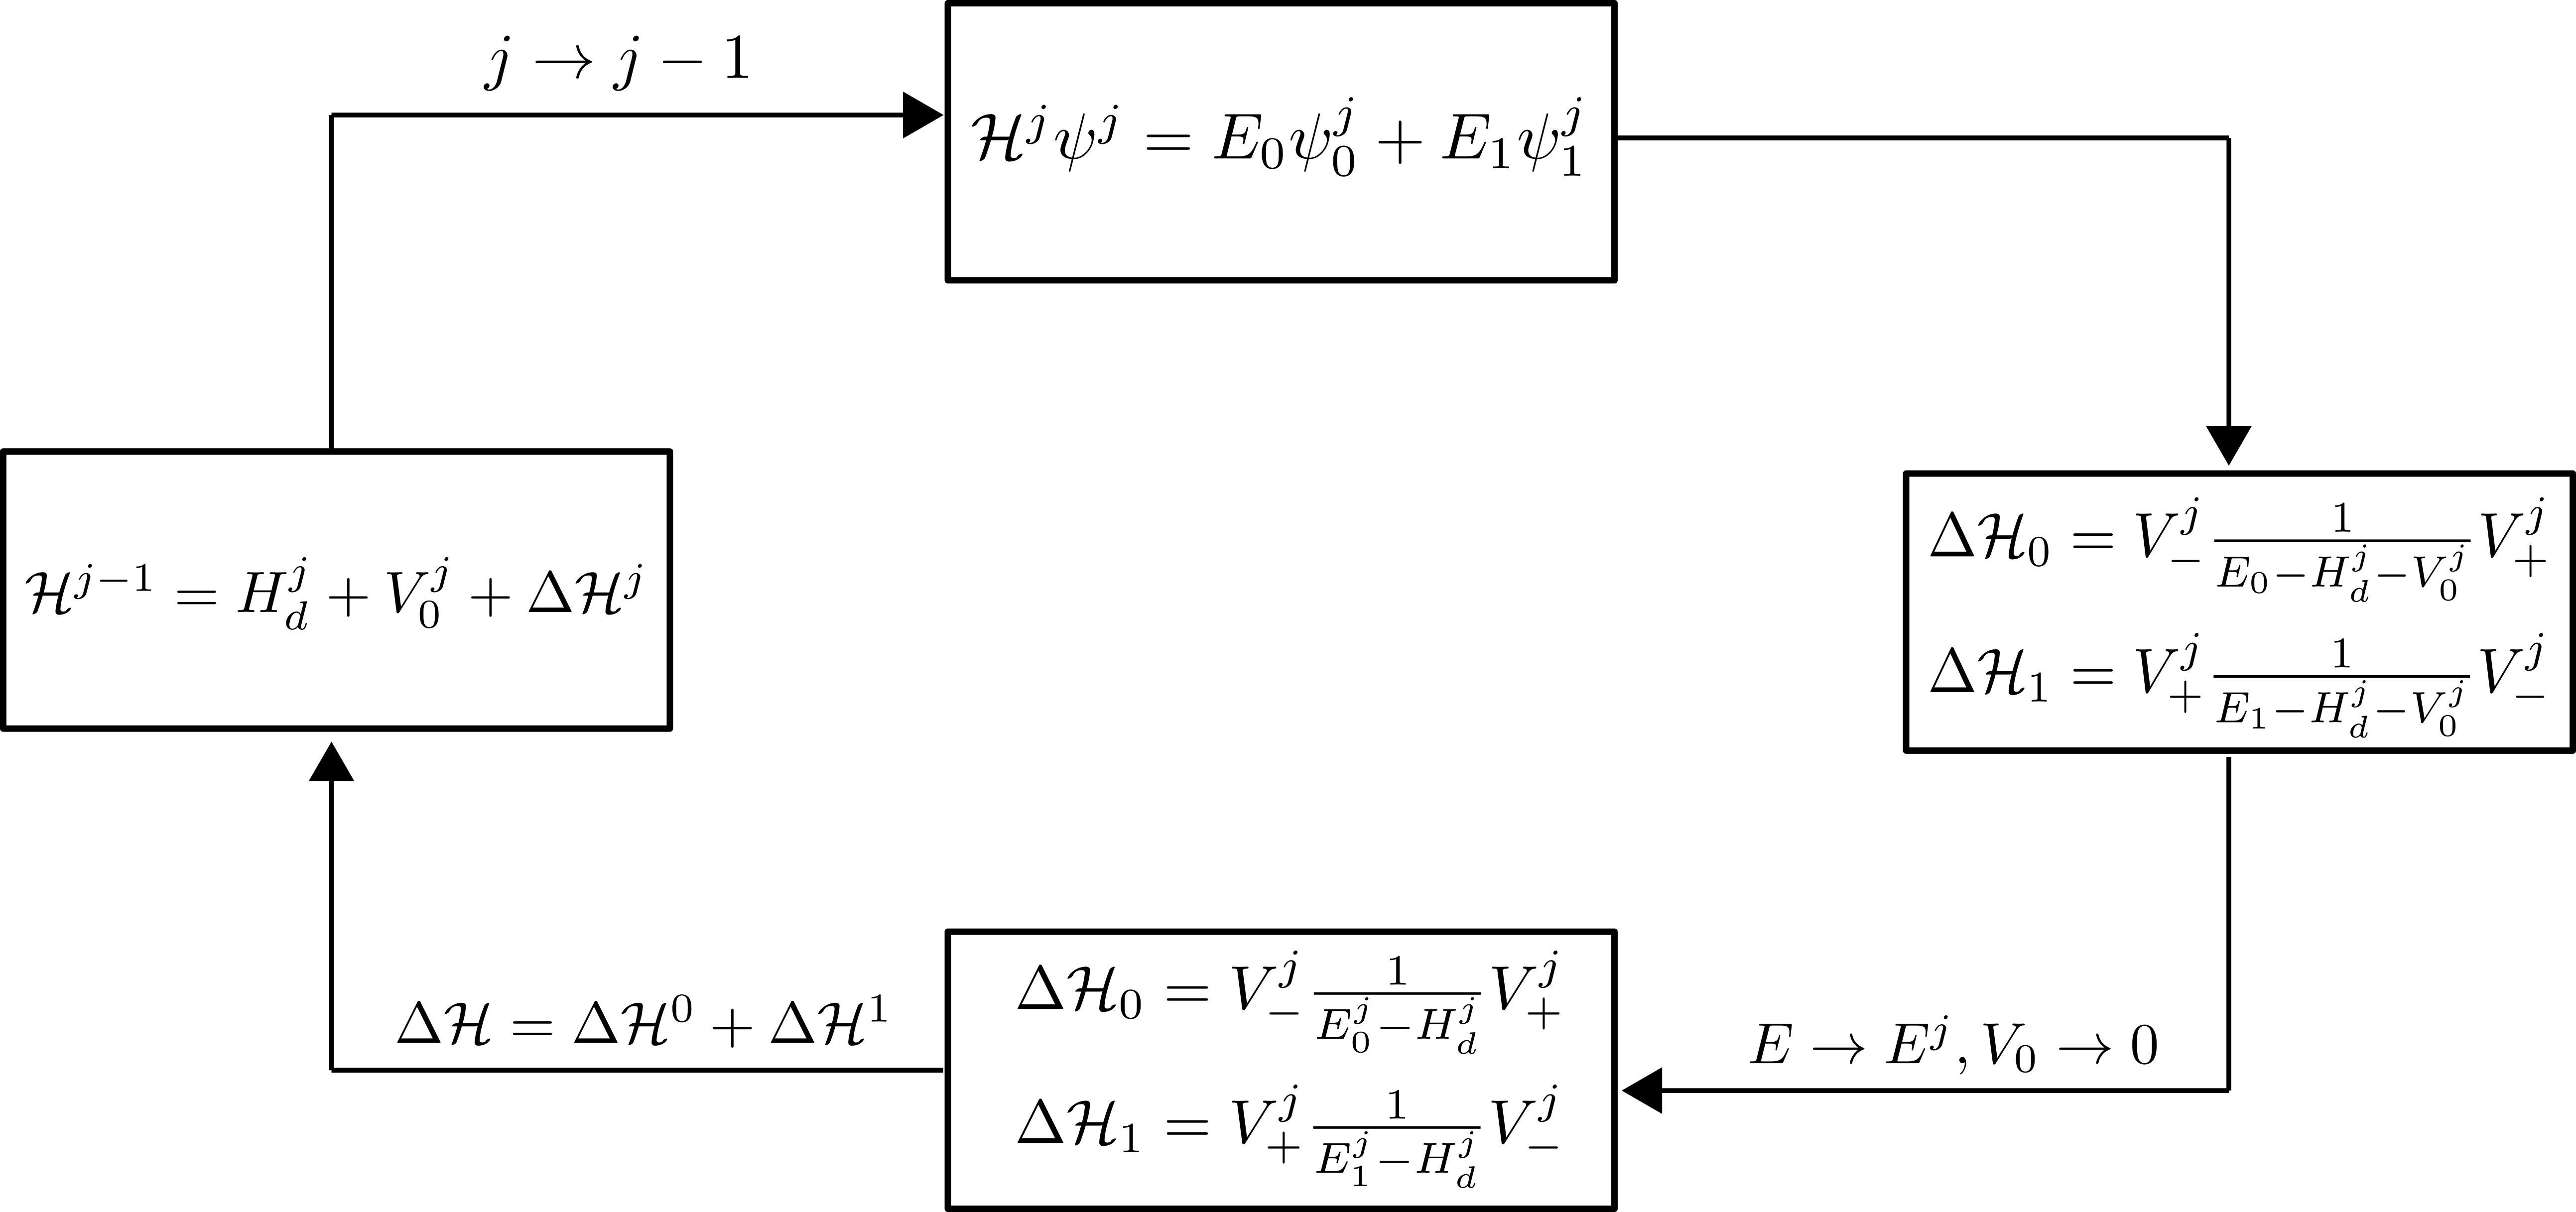
\includegraphics[scale=0.34]{pms-flowchart.png}
    \caption{Flow chart of "Poor Man's" scaling algorithm}
    \label{pmsflow}
\end{figure}
\\\\\textbf{Some conclusions}:
\begin{itemize}
\item The \textit{only} difference in the formalism of PMS and URG is that while PMS uses the exact energy eigenvalue \(E\) to parameterise the flow, URG uses a general intermediate decoupled Hamiltonian to do the same. Since the \(E\) is also, technically, an intermediate decoupled Hamiltonian (it is the final Hamiltonian), PMS can be seen as an URG but with a specific choice for the paramter.
\item In practise, PMS replaces \(E-V_0\) with the diagonal part of the initial state at the current step of the RG. We are talking about the energy of the initial state, not the intermediate state. This is because, from eq.~\ref{problem}, \(E\) is the energy of the initial state on which \(V_\pm\) act. 
\item The ideal solution would have been to substitute the exact energy and the total scattering term \(V\), but since we do not know \(E\) and keeping the \(V\) would make the thing untractable, we use our current best guess (renormalised diagonal part). As the RG flows, both \(E_j\) and \(V\) flow, such that at the fixed point, \(V\) becomes zero (scattering terms get removed) and \(E_j\) morphs into the exact \(E\). 
\item In practise, URG replaces the \(\hat \omega\) with a guess for the final energy \(E\). This however ignores the renormalization of \(\hat \omega\). A better approach would be to replace it with \(E_j\), following PMS. That would act like the one-particle renormalization of \(\hat \omega\).
\item PMS usually drops any diagonal component of the scattering from the denominator. For example, in the PMS of the Kondo model by Anderson \cite{Anderson} or that of the anisotropic power law Kondo model by Chenge et.al \cite{tatha}, they do not keep the term \(J_z S_d^z s^z\) in the denominator although it is number(spin) conserving. Such terms are kept in the denominator of the URG though. It must be mentioned however that ref.~\cite{raja} \textit{does} bring a diagonal charge-charge interaction in the denominator in the PMS of the extended Anderson model.
\end{itemize}
\section{Schrieffer-Wolff transformation (SWT)}
\subsection{Formalism}
We have a general Hamiltonian
\begin{equation}\begin{aligned}
\mathcal{H} = \mathcal{H}_0 + \mathcal{H}_X
\end{aligned}\end{equation}
\(\mathcal{H}_0\) is diagonal w.r.t a particular degree of freedom. \(V\) is off-diagonal w.r.t that same degree of freedom. Let \(S\) be an \textit{anti-Hermitian} and \textit{off-diagonal} operator. \(U = e^S\) is then a unitary transformation.
\begin{equation}\begin{aligned}
	U \mathcal{H} U^\dagger &= e^S \left(\mathcal{H}_0 + \mathcal{H}_X\right)e^{-S}\\
				&= \left(\cosh\left(S\right) + \sinh\left(S\right)\right)\left(\mathcal{H}_0 + \mathcal{H}_X\right)\left(\cosh\left(S\right) - \sinh\left(S\right)\right)\\
         &= H_1 + H_2
\end{aligned}\end{equation}
where \(H_1\) is diagonal and \(H_2\) is off-diagonal.
\begin{equation}\begin{aligned}
	H_1=\cosh\left(S\right) \mathcal{H}_0 \cosh\left(S\right) - \sinh\left(S\right) \mathcal{H}_0 \sinh\left(S\right) -\cosh\left(S\right) \mathcal{H}_X \sinh\left(S\right)\\
	+\sinh\left(S\right) \mathcal{H}_X \cosh\left(S\right)\\
	H_2 = - \cosh\left(S\right) \mathcal{H}_0 \sinh\left(S\right) + \sinh\left(S\right) \mathcal{H}_0 \cosh\left(S\right) +\cosh\left(S\right) \mathcal{H}_X \cosh\left(S\right)\\
	-\sinh\left(S\right) \mathcal{H}_X \sinh\left(S\right)
\end{aligned}\end{equation}
The decoupling condition is \(H_2=0\).
\\\\For small \(S\), we have \(\sinh S \sim S\) and \(\cosh S \sim 1 + \frac{1}{2} S^2\). Therefore, the off-diagonal part, up to second order, is 
\begin{equation}\begin{aligned}
	H_2 = -\mathcal{H}_0 S + S \mathcal{H}_0 + \mathcal{H}_X + O(S^3) = \left[S,\mathcal{H}_0\right] + \mathcal{H}_X
\end{aligned}\end{equation}
The second order decoupling condition is thus
\begin{equation}\begin{aligned}
	\label{dec_cond}
	\left[S,\mathcal{H}_0\right] = -\mathcal{H}_X
\end{aligned}\end{equation}
The effective Hamiltonian is what remains, \(H_1\). That becomes, at second order,
\begin{equation}\begin{aligned}
	H_1 &= \left(1 + \frac{1}{2} S^2\right) \mathcal{H}_0 \left(1 + \frac{1}{2} S^2\right) - S \mathcal{H}_0 S -\left(1 + \frac{1}{2} S^2\right) \mathcal{H}_X S + S \mathcal{H}_X \left(1 + \frac{1}{2} S^2\right)\\
    &= \mathcal{H}_0 + \frac{1}{2} \left\{S^2, \mathcal{H}_0\right\} - S \mathcal{H}_0 S - \mathcal{H}_X S + S \mathcal{H}_X + O(S^3)\\
    &= \mathcal{H}_0 + \frac{1}{2} S\left[S, \mathcal{H}_0\right] - \frac{1}{2} \left[S, \mathcal{H}_0\right]S  + \left[S,\mathcal{H}_X\right] + O(S^3)\\
    &= \mathcal{H}_0 + \frac{1}{2} \left[S,\left[S, \mathcal{H}_0\right]\right] + \left[S,\mathcal{H}_X\right] + O(S^3)\\
    &= \mathcal{H}_0 + \frac{1}{2} \left[S,-\mathcal{H}_X\right] + \left[S,\mathcal{H}_X\right] + O(S^3)\\
    &= \mathcal{H}_0 + \frac{1}{2}\left[S,\mathcal{H}_X\right] + O(S^3)\\
\end{aligned}\end{equation}
Avoiding the perturbative route, we can take \(S = \frac{\pi}{4}\left(\eta^\dagger - \eta\right)\), where \(\eta\) and its conjugate are non-perturbative and Fermionic - they satisfy \(\eta^2 = {\eta^\dagger}^2 = 0\) and \(\left\{\eta,\eta^\dagger\right\}=1\). We can then write
\begin{equation}\begin{aligned}
	e^S &= \exp\left\{\frac{\pi}{4}\left(\eta^\dagger - \eta\right)\right\} \\
	    &= 1 + \left(\eta^\dagger - \eta\right)\frac{\pi}{4} + \frac{1}{2!}\left(\eta^\dagger - \eta\right)^2\left(\frac{\pi}{4}\right)^2 + \frac{1}{3!}\left(\eta^\dagger - \eta\right)^3\left(\frac{\pi}{4}\right)^3 + ...\\
	    &= 1 + \left(\eta^\dagger - \eta\right)\frac{\pi}{4} - \frac{1}{2!}\left(\frac{\pi}{4}\right)^2 - \frac{1}{3!}\left(\eta^\dagger - \eta\right)\left(\frac{\pi}{4}\right)^3 + \frac{1}{4!}\left(\frac{\pi}{4}\right)^4 + ...\\
	    &= \cos \frac{\pi}{4} + \left(\eta^\dagger - \eta\right)\sin\frac{\pi}{4}\\
	    &= \frac{1}{\sqrt 2}\left(1 + \eta^\dagger - \eta\right)
\end{aligned}\end{equation}
There we used
\begin{equation}\begin{aligned}
	\left(\eta^\dagger - \eta\right)^2 = {\eta^\dagger}^2 + \eta^2 - \left\{\eta^\dagger,\eta\right\} = -1 &&\left[\because\eta^2 = {\eta^\dagger}^2=0\right]
\end{aligned}\end{equation}
and hence
\begin{equation}\begin{aligned}
	\left(\eta^\dagger - \eta\right)^3 = -1\left(\eta^\dagger - \eta\right)
\end{aligned}\end{equation}
and so on. This simplification allows us to write
\begin{equation}\begin{aligned}
	\label{cossin}
	\cosh S = \frac{1}{2}\left[e^S + e^{-S}\right] = \frac{1}{2\sqrt 2}\left(1 + \eta^\dagger - \eta + 1 - \eta^\dagger + \eta\right) = \frac{1}{\sqrt 2}
\end{aligned}\end{equation}
and
\begin{equation}\begin{aligned}
	\sinh S = \frac{1}{2}\left[e^S - e^{-S}\right] = \frac{1}{2\sqrt 2}\left(1 + \eta^\dagger - \eta - 1 + \eta^\dagger - \eta\right) = \frac{1}{\sqrt 2}\left(\eta^\dagger - \eta\right)
\end{aligned}\end{equation}
The off-diagonal part now becomes
\begin{equation}\begin{aligned}
	H_2 = \frac{1}{2}\left(\mathcal{H}_X - \eta^\dagger \mathcal{H}_X \eta^\dagger - \eta \mathcal{H}_X \eta + \left[\eta^\dagger - \eta, \mathcal{H}_0\right]\right)
\end{aligned}\end{equation}
The vanishing of this quantity is now the decoupling condition, and is also given in eq 16 of ref.~\cite{anirbanurg1}.
\\\\To look for a decoupling condition similar to eq.~\ref{dec_cond}, we can re-express the \(\cosh\) and \(\sinh\) in eq.~\ref{cossin} in terms of \(S\), by substituting \(\eta^\dagger - \eta = \frac{4}{\pi}S\):
\begin{equation}\begin{aligned}
\cosh S = \frac{1}{\sqrt 2},\text{ and } \sinh S = \frac{4}{\sqrt 2 \pi}S
\end{aligned}\end{equation}
That gives
\begin{equation}\begin{aligned}
	H_2 = \frac{1}{2}\left(\frac{4}{\pi}\left[S,\mathcal{H}_0\right] + \mathcal{H}_X - \frac{16}{\pi^2}S \mathcal{H}_X S\right)
\end{aligned}\end{equation}
The decoupling condition becomes
\begin{equation}\begin{aligned}
	\left[S,\mathcal{H}_0\right] = -\frac{\pi}{4}\mathcal{H}_X + \frac{4}{\pi}S \mathcal{H}_X S
\end{aligned}\end{equation}
This can be compared to the second order condition: \(\left[S,\mathcal{H}_0\right] = -\mathcal{H}_X\). We  can also write the effective Hamiltonian for this non-perturbative case.
\begin{equation}\begin{aligned}
	U\mathcal{H} U^\dagger = H_1 = \frac{1}{2} \mathcal{H}_0 - \frac{4}{\pi^2}S\mathcal{H}_0 S  + \frac{2}{\pi}\left[S,\mathcal{H}_X\right]
\end{aligned}\end{equation}
The differences between the perturbative and non-perturbative ways are summarized in table \ref{comparison}.
\begin{table}
% \def\tabcolsep=10pt
\centering
\begin{tabular}{|c|c|c|}
    \hline
        &renormalization&decoupling condition\\
    \hline
	SWT&\(\frac{1}{2} \left[S,\mathcal{H}_X\right]\)&\(\left[S,\mathcal{H}_0\right] = -\mathcal{H}_X\)\\
	URG&\(\frac{2}{\pi}\left[S,\mathcal{H}_X\right]\)&\(\left[S,\mathcal{H}_0\right] = -\frac{\pi}{4}\mathcal{H}_X + \frac{4}{\pi}S \mathcal{H}_X S\)\\
    \hline
\end{tabular}
    \caption{Comparison of perturbative and non-perturbative canonical transformations}
    \label{comparison}
\end{table}
There appear to be two differences between these decoupling conditions: (a)  a pre-factor of \(\frac{\pi}{4}\) for the first term on the right hand side, and (b) the altogether new second term on the right hand side. Both are outcomes of the non-perturbative nature of URG. This offers evidence that the physics captured by the effective Hamiltonian (and its associated low-energy many-particle Hilbert space) obtained from URG lies well beyond that obtained from SWT. Further, it shows that the SWT can only be justified as an expansion in a small parameter (say, $\frac{1}{U}$) in the Anderson impurity problem), followed by a truncation of the BCH expansion and a projection onto a particular low-energy subspace. The truncation and projection are adopted simultaneously, and appear to impose the limit of \(U = \infty\) by hand. The URG flow never attains such a limit, thus suggesting that there exists a lot of interesting physics that could potentially be lost in the SWT procedure. Further, the projection finally applied within SWT means that we can never recover what is thrown away. This is again not the case with URG.
\subsection{Obtaining renormalization via Schrieffer-Wolff transformation - comparison with "poor man's scaling" and URG}
Similar to the situation in Poor Man's scaling, one can visualize two set of states and let \(\mathcal{H}_X = V_+ + V_-\) be the scattering that connects them and hence the one we want to kill. Let \(S\) be of the form 
\begin{equation}\begin{aligned}
	S = \sum_{ij}\left[s\ket{\phi_1^i}\bra{\phi_0^j} - s^\dagger\ket{\phi_0^j}\bra{\phi_1^i}\right]
\end{aligned}\end{equation}
This form is of course chosen to make \(S\) anti-Hermitian and off-diagonal. The part \(s\) can be determined from the decoupling condition:
\begin{equation}\begin{aligned}
	-\mathcal{H}_X = \left[S, H_0\right] = S H_0 - H_0 S
\end{aligned}\end{equation}
Multiplying with \(\bra{\phi_0^a}\) and \(\ket{\phi_1^b}\) from the left and right respectively gives
\begin{equation}\begin{aligned}
-\bra{\phi_0^a}V + V^\dagger\ket{\phi_1^b} &= \bra{\phi_0^a}S H_0 - H_0 S\ket{\phi_1^b}\\
\end{aligned}\end{equation}
Since \(V^\dagger\) acts on \(\ket{0}\), it will not affect the LHS. Also, \(\bra{\phi_0^a}V\ket{\phi_1^b} = V_{ab}\). If we now consider only the diagonal part of \(H_0\), we can write \(H_0 (\ket{\phi_0^a},\ket{\phi_1^b}) = (E_{0,a}\ket{\phi_0^a},E_{1,b}\ket{\phi_1^b}))\). We then get
\begin{equation}\begin{aligned}
	-V_{ab} &= \bra{\phi_0^a}\sum_i\left[S\ket{\phi_1^i}\bra{\phi_1^i} H_0 - H_0 \ket{\phi_0^i}\bra{\phi_0^i}S\right]\ket{\phi_1^b}\\
		&= \sum_i\left[S_{ai}E_1^i \delta_{bi} - E^i_0 \delta_{ai}S_{ib}\right]\\
    &= S_{ab}E_1^b  - E^a_0 S_{ab}\\
\implies S_{ab} &= \frac{V_{ab}}{E_0^a - E_1^b}
\end{aligned}\end{equation}
where we defined \(\bra{\phi_0^x}S\ket{\phi_1^y} = S_{xy}\). The total generator is
\begin{equation}\begin{aligned}
	\label{swtgen}
	S &= \sum_{ij}\left[S_{ij}\ket{\phi_0^i}\bra{\phi_1^j} - S_{ij}^\dagger\ket{\phi_1^j}\bra{\phi_0^i}\right]\\
	  &= \sum_{ij}\frac{1}{E_0^i - E_1^j}\left[V_{ij}\ket{\phi_0^i}\bra{\phi_1^j} - V^\dagger_{ij}\ket{\phi_1^j}\bra{\phi_0^i}\right]\\
\end{aligned}\end{equation}
The renormalization is thus
\begin{equation}\begin{aligned}
	\Delta \mathcal{H} &= \frac{1}{2} \left[S,\mathcal{H}_X\right]\\
			   &= \frac{1}{2} \sum_{ij,kl}\left[\frac{1}{E_0^i - E_1^j}\left(V_{ij}\ket{\phi_0^i}\bra{\phi_1^j} - V^\dagger_{ij}\ket{\phi_1^j}\bra{\phi_0^i}\right), V_{kl} \ket{\phi_0^k}\bra{\phi_1^l}+ V^\dagger_{kl} \ket{\phi_1^l}\bra{\phi_0^k}\right]\\
                  &= \frac{1}{2} \sum_{ij,kl}\left[\frac{1}{E_0^i - E_1^j}\left(V_{ij}V^\dagger_{kl}\ket{\phi_0^i}\bra{\phi_0^k}\delta_{jl} - V^\dagger_{ij}V_{kl}\ket{\phi_1^j}\bra{\phi_1^l}\delta_{ik}\right.\right.\\
                  &\quad\left.\left.- V^\dagger_{kl}V_{ij}\ket{\phi_1^l}\bra{\phi_1^j}\delta_{ki} + V_{kl}V^\dagger_{ij}\ket{\phi_0^k}\bra{\phi_0^i}\delta_{lj}\right)\right]\\
                  &= \frac{1}{2} \sum_{ijk}\left[\frac{1}{E_0^i - E_1^j}\left(V_{ij}V^\dagger_{kj}\ket{\phi_0^i}\bra{\phi_0^k} - V^\dagger_{ij}V_{ik}\ket{\phi_1^j}\bra{\phi_1^k}- V^\dagger_{ik}V_{ij}\ket{\phi_1^k}\bra{\phi_1^j} + V_{kj}V^\dagger_{ij}\ket{\phi_0^k}\bra{\phi_0^i}\right)\right]\\
		  &= \frac{1}{2} \sum_{ijk}\left[\left(\frac{1}{E_0^i - E_1^j} + \frac{1}{E_0^k - E_1^j}\right)V_{ij}V^\dagger_{kj}\ket{\phi_0^i}\bra{\phi_0^k} - \left(\frac{1}{E_0^i - E_1^j} + \frac{1}{E_0^i - E_1^k}\right)V^\dagger_{ij}V_{ik}\ket{\phi_1^j}\bra{\phi_1^k}\right]\\
\end{aligned}\end{equation}
This is the same as the PMS result eq.~\ref{pmsren}. It is easy to see that since this transformation is unitary, it has zero trace so as to preserve the trace of the Hamiltonian:
\begin{equation}\begin{aligned}
	\text{Tr}\left[\mathcal{H}\right] &= \sum_{l}\left(\bra{\phi_0^l} + \bra{\phi_1^l}\right)\Delta \mathcal{H}\left(\ket{\phi_0^l} + \ket{\phi_1^l}\right)\\
		&= \frac{1}{2} \sum_{jl}\frac{2}{E_0^l - E_1^j}V_{lj}V^\dagger_{lj} - \frac{1}{2} \sum_{ji}\frac{2}{E_0^i - E_1^l}V^\dagger_{il}V_{il}\\
		&= 0
\end{aligned}\end{equation}
\\\\We can also make a comparison to the renormalization obtained from URG.
\begin{equation}\begin{aligned}
	\Delta \mathcal{H} &= \frac{1}{2}\left[\eta^\dagger - \eta,\mathcal{H}\right]
\end{aligned}\end{equation}
where 
\begin{equation}\begin{aligned}
\eta &= \frac{1}{\omega - \mathcal{H}^d}\sum_{ij}V_{ij}\ket{\phi_0^i}\bra{\phi_1^j} = \sum_{ij}\frac{1}{\omega_1^j - E_0^i}V_{ij}\ket{\phi_0^i}\bra{\phi_1^j}\\
\implies \eta^\dagger &= \sum_{ij}\frac{1}{\omega_1^j - E_0^i}V^\dagger_{ij}\ket{\phi_1^j}\bra{\phi_0^i}\\
\implies \eta^\dagger - \eta &= \sum_{ij}\frac{1}{\omega_1^j - E_0^i}\left(V^\dagger_{ij}\ket{\phi_1^j}\bra{\phi_0^i} - V_{ij}\ket{\phi_0^i}\bra{\phi_1^j}\right)\\
\end{aligned}\end{equation}
This can be thought of as the generator for the unitary transformations of URG. Comparing with the generator \(S\) of eq.~\ref{swtgen}, the prescription to go from URG to SWT is to replace \(\omega_1^j \to E_1^j\). Doing a similar calculation gives
\begin{equation}\begin{aligned}
	\Delta \mathcal{H}_{URG} = \frac{1}{2} \sum_{ijk}\left[\left(\frac{1}{E_0^i - \omega_1^j} + \frac{1}{E_0^k - \omega_1^j}\right)V_{ij}V^\dagger_{kj}\ket{\phi_0^i}\bra{\phi_0^k}\right.\\
	- \left.\left(\frac{1}{E_0^i - \omega_1^j} + \frac{1}{E_0^i - \omega_1^k}\right)V^\dagger_{ij}V_{ik}\ket{\phi_1^j}\bra{\phi_1^k}\right]\\
\end{aligned}\end{equation}

\section{A comparison of URG, SWT and PMS on the Anderson model}
The SWT for the single-impurity Anderson model is briefly sketched below. In order to decouple a state \(q\beta\) from the SIAM (\(\epsilon_q > 0\)) , we take an ansatz \(S = (A + B\hat n_{d\overline\beta})(c^\dagger_{q\beta}c_{d\beta} - \text{h.c.})\). Plugging this into the decoupling condition gives
\begin{equation}\begin{aligned}
	-\epsilon_q\left(A + B\hat n_{d\overline\beta}\right) + \epsilon_d\left(A + B\hat n_{d\overline\beta}\right) + U\left(A + B\right)\hat n_{d\overline\beta} = -V
\end{aligned}\end{equation}
which gives
\begin{equation}\begin{aligned}
	S = V\left[\frac{1 - \hat n_{d\overline\beta}}{\epsilon_q - \epsilon_d} + \frac{\hat n_{d\overline\beta}}{\epsilon_q - \epsilon_d - U}\right] (c^\dagger_{q\beta}c_{d\beta} - \text{h.c.})
\end{aligned}\end{equation}
The remaining diagonal part constitutes the effective Hamiltonian.
\begin{equation}\begin{aligned}
	U\mathcal{H} U^\dagger = H_1 &= \mathcal{H}_0 + \frac{1}{2} \left\{\mathcal{H}_0, S^2\right\} - S \mathcal{H}_0 S + \left[S,\mathcal{H}_X\right]\\
				     &=\mathcal{H}_0 + \frac{1}{2} \left[\left[\mathcal{H}_0, S\right],S\right] + \left[S,\mathcal{H}_X\right]\\
				     &=\mathcal{H}_0 + \frac{1}{2} \left[\mathcal{H}_X,S\right] + \left[S,\mathcal{H}_X\right]\\
				     &=\mathcal{H}_0 + \frac{1}{2} \left[S,\mathcal{H}_X\right]
\end{aligned}\end{equation}
For the SIAM (and noting that we are decoupling \(q\beta\)), the two parts are
\begin{equation}\begin{aligned}
	\mathcal{H}_0 &= \sum_{k\sigma}\epsilon_k \hat n_{k\sigma} + \epsilon_d \hat n_d + U\hat n_{d\uparrow}\hat n_{d\downarrow} + \sum_{k\sigma \neq q\beta}\left(c^\dagger_{k\sigma}c_{d\sigma} + \text{h.c.}\right)\\
\mathcal{H}_X &= c^\dagger_{q\beta}c_{d\beta} + \text{h.c.} 
\end{aligned}\end{equation}
The renormalization in the effective Hamiltonian from decoupling a high energy particle state is thus
\begin{equation}\begin{aligned}
	\frac{1}{2} \left[S,\mathcal{H}_X\right]\bigg\vert_{\hat n_{q\beta}=0} &= |V|^2\left[\frac{1 - \hat n_{d\overline\beta}}{\epsilon_q - \epsilon_d} + \frac{\hat n_{d\overline\beta}}{\epsilon_q - \epsilon_d - U}\right]\left[\hat n_{q\beta}\left(1 - \hat n_{d\beta}\right) - \hat n_{d\beta}\left(1 - \hat n_{q\beta}\right)\right]\bigg\vert_{\hat n_{q\beta}=0}\\
									       &=-\hat n_{d\beta}|V|^2\left[\frac{1 - \hat n_{d\overline\beta}}{\epsilon_q - \epsilon_d} + \frac{\hat n_{d\overline\beta}}{\epsilon_q - \epsilon_d - U}\right]
\end{aligned}\end{equation}
In the last step, we put \(\hat n_{q\beta}=0\) because previously we assumed \(\epsilon_q>0\) and high energy virtual excitations above the Fermi surface must necessarily be vacant in the initial state (at \(T=0\)). We can obtain the renormalization from decoupling a high energy \textit{hole} state directly from this expression, just by choosing \(\hat n_{q\beta}=1\) and setting \(\epsilon_q \to -\epsilon_q\).
\begin{equation}\begin{aligned}
	\frac{1}{2} \left[S,\mathcal{H}_X\right]\bigg\vert_{\hat n_{q\beta}=1} &=-\left(1 - \hat n_{d\beta}\right)|V|^2\left[\frac{1 - \hat n_{d\overline\beta}}{\epsilon_q + \epsilon_d} + \frac{\hat n_{d\overline\beta}}{\epsilon_q + \epsilon_d + U}\right]
\end{aligned}\end{equation}
These two results - the renormalization in the particle and hole sectors - is identical to the result (see \cite{hewson}) obtained from PMS of the SIAM. The renormalizations in the various energy levels of the impurity can be read off now, after summing over all states in the interval we are decoupling.
\begin{equation}\begin{aligned}
\Delta E_2 &= -2\sum_{q}\frac{|V_q|^2}{\epsilon_q - \epsilon_d - U}\\
\Delta E_1 &= -\sum_{q}\frac{|V_q|^2}{\epsilon_q - \epsilon_d} - \sum_{q}\frac{|V_q|^2}{\epsilon_q + \epsilon_d + U}\\
\Delta E_0 &= -2\sum_{q}\frac{|V_q|^2}{\epsilon_q + \epsilon_d}\\
\end{aligned}\end{equation}
This can be compared with the URG result, eq.~\ref{urg-siam},
\begin{equation}\begin{aligned}
\Delta E_2 &= 2\sum_{q}\frac{|V_q|^2}{\omega - \frac{1}{2}\epsilon_q + \epsilon_d + U}\\
\Delta E_1 &= \sum_{q}\frac{|V_q|^2}{\omega - \frac{1}{2}\epsilon_q - \epsilon_d - U} + \sum_{q}\frac{|V_q|^2}{\omega - \frac{1}{2}\epsilon_q + \epsilon_d}\\
\Delta E_0 &= 2\sum_{q}\frac{|V_q|^2}{\omega - \frac{1}{2}\epsilon_q - \epsilon_d}\\
\end{aligned}\end{equation}
We can transform the URG result to the SWT result if we ignore the effect of the quantum fluctuations in \(\omega\) (arising from the presence of the off-diagonal term \(\mathcal{H}^i\)) and replace it with the renormalised diagonal value of \(-\frac{1}{2}\epsilon_q\). This means that SWT tracks the effect of the off-diagonal terms only in the numerator. Of course, all this assumes we are doing an iterative SWT instead of a one-shot SWT; the latter is the conventional way. A second difference is that URG has a Green's function like structure in the renormalization such that a fixed point is reached when the diagonal part \(\mathcal{H}^d\) matches one of the eigenvalues of \(\omega\) (see \ref{match}). SWT does not have such a fixed point structure.
\\\\Another point to note is that decoupling a single electron does not generate all the charge-charge or spin-spin interactions that come out when one performs a one-shot SWT. This implies that such terms are a result of decoupling the non-local interactions of the impurity (it is talking to all the mobile electrons), and cannot be generated when we remove just the local interactions of the mobile electrons. Instead, if one performs a URG in which we non-perturbatively kill the 2-point vertices in the SIAM, such 4-point vertices are generated. This is shown in the next subsection.
\section{Deriving the Kondo model from the Anderson model via a one-shot URG}\label{SWT from URG}
Here we will show how we can obtain the spin-spin interaction of the Kondo model by performing a one-shot URG on the SIAM. This should justify that the action of performing an SWT is analogous to decoupling the whole band via URG. \\\\There are three departures from the conventional way of doing URG (or PMS).
\begin{itemize}
    \item We will be severing the connections of the impurity with all the mobile electrons in one-shot, and not iteratively.
    \item We will have to trivialize the quantum fluctuation operator \(\hat \omega\) by replacing it with the diagonal part of the initial state energy.
\end{itemize}
Since we are decoupling the whole band, the off-diagonal part that we want to remove is
\begin{equation}\begin{aligned}
	\mathcal{H}^I = \sum_{k\sigma}\left[V_k c^\dagger_{k\sigma}c_{d\sigma}+\text{h.c.}\right]
\end{aligned}\end{equation}
The diagonal part is the rest of the Hamiltonian.
\begin{equation}\begin{aligned}
\mathcal{H}^d &= \sum_{k\sigma}\epsilon_k\hat n_{k\sigma} + \epsilon_d\hat n_d + U\hat n_{d\uparrow}\hat n_{d\downarrow}\\
&= \sum_{k\sigma}\epsilon_k\tau_{k\sigma} + \epsilon_d\hat n_d + U\hat n_{d\uparrow}\hat n_{d\downarrow}\\
\end{aligned}\end{equation}
Following eq.~\ref{renurg}, the renormalization is
\begin{equation}\begin{aligned}
	\Delta \mathcal{H} = \frac{1}{2}\left[\eta^\dagger - \eta, \mathcal{H}_X\right]
\end{aligned}\end{equation}
The transition operator \(\eta\) is
\begin{equation}\begin{aligned}
	\label{swturg}
\eta &= \frac{1}{\omega - \mathcal{H}^d}\sum_{k\sigma}V^*_k c^\dagger_{d\sigma}c_{k\sigma}\\
     &= \sum_{k\sigma}\frac{1}{\omega + \frac{1}{2}\epsilon_k - \epsilon_d - \left(\epsilon_d + U\right)\hat n_{d\overline\sigma}}V^*_k c^\dagger_{d\sigma}c_{k\sigma}\\
     &= \sum_{k\sigma}\left[\frac{\hat n_{d\overline\sigma}}{\omega_1 + \frac{1}{2}\epsilon_k - 2\epsilon_d - U} + \frac{1 - \hat n_{d\overline\sigma}}{\omega_0 + \frac{1}{2}\epsilon_k - \epsilon_d}\right]V^*_k c^\dagger_{d\sigma}c_{k\sigma}\\
     &= \sum_{k\sigma}\left[\frac{\hat n_{d\overline\sigma}}{E_k^1} + \frac{1 - \hat n_{d\overline\sigma}}{E_k^0}\right]V^*_k c^\dagger_{d\sigma}c_{k\sigma}\\
\end{aligned}\end{equation}
where \(E_k^1 = \omega_1 + \frac{1}{2}\epsilon_k - 2\epsilon_d - U\) and \(E_k^0 = \omega_0 + \frac{1}{2}\epsilon_k - \epsilon_d\). The total generator is therefore
\begin{equation}\begin{aligned}
	\eta^\dagger - \eta = \sum_{k\sigma}\left[\frac{\hat n_{d\overline\sigma}}{E_k^1} + \frac{1 - \hat n_{d\overline\sigma}}{E_k^0}\right] \left(V_k c^\dagger_{k\sigma}c_{d\sigma} - V^*_k c^\dagger_{d\sigma}c_{k\sigma}\right)
\end{aligned}\end{equation}
The renormalization is
\begin{equation}\begin{aligned}
	\Delta \mathcal{H}(\omega_1,\omega_0) = \frac{1}{2}\sum_{kq\sigma\alpha}\left[\left(\frac{\hat n_{d\overline\sigma}}{E_k^1} + \frac{1 - \hat n_{d\overline\sigma}}{E_k^0}\right)\left(V_k c^\dagger_{k\sigma}c_{d\sigma} - V^*_k c^\dagger_{d\sigma}c_{k\sigma}\right),V_q c^\dagger_{q\alpha}c_{d\alpha} + V_q^* c^\dagger_{d\alpha}c_{q\alpha}\right]
\end{aligned}\end{equation}
The summation has two parts, \(\Delta_{1,2}\) - one where \(\sigma=\alpha\) and another where \(\sigma=\overline\alpha\). The first part \(\Delta_1\) gives
\begin{equation}\begin{aligned}
	\Delta_1 &=\frac{1}{2}\sum_{kq\sigma=\alpha}\left[\left(\frac{\hat n_{d\overline\sigma}}{E_k^1} + \frac{1 - \hat n_{d\overline\sigma}}{E_k^0}\right)\left(V_k c^\dagger_{k\sigma}c_{d\sigma} - V^*_k c^\dagger_{d\sigma}c_{k\sigma}\right),V_q c^\dagger_{q\sigma}c_{d\sigma} + V_q^* c^\dagger_{d\sigma}c_{q\sigma}\right]\\
		 &=\frac{1}{2}\sum_{kq\sigma}\left(\frac{\hat n_{d\overline\sigma}}{E_k^1} + \frac{1 - \hat n_{d\overline\sigma}}{E_k^0}\right)\left[V_k c^\dagger_{k\sigma}c_{d\sigma} - V^*_k c^\dagger_{d\sigma}c_{k\sigma},V_q c^\dagger_{q\sigma}c_{d\sigma} + V_q^* c^\dagger_{d\sigma}c_{q\sigma}\right]\\
		 &=\frac{1}{2}\sum_{kq\sigma}\left(\frac{\hat n_{d\overline\sigma}}{E_k^1} + \frac{1 - \hat n_{d\overline\sigma}}{E_k^0}\right)\left\{V_k V_q^*\left[c^\dagger_{k\sigma}c_{d\sigma}, V_q^* c^\dagger_{d\sigma}c_{q\sigma}\right] - V^*_k V_q \left[c^\dagger_{d\sigma}c_{k\sigma},c^\dagger_{q\sigma}c_{d\sigma}\right]\right\}\\
		 &=\frac{1}{2}\sum_{kq\sigma}\left(\frac{\hat n_{d\overline\sigma}}{E_k^1} + \frac{1 - \hat n_{d\overline\sigma}}{E_k^0}\right)\left\{V_k V_q^*\left[c^\dagger_{k\sigma}c_{d\sigma}, V_q^* c^\dagger_{d\sigma}c_{q\sigma}\right] + V^*_k V_q \left[c^\dagger_{q\sigma}c_{d\sigma},c^\dagger_{d\sigma}c_{k\sigma}\right]\right\}\\
		 &=\frac{1}{2}\sum_{kq\sigma}\left[\hat n_{d\overline\sigma}\left(\frac{1}{E_k^1} + \frac{1}{E_q^1}\right) + \left(1 - \hat n_{d\overline\sigma}\right)\left(\frac{1}{E_k^0} + \frac{1}{E_q^0}\right)\right]V_k V_q^*\left[c^\dagger_{k\sigma}c_{d\sigma}, c^\dagger_{d\sigma}c_{q\sigma}\right]\\
		 &=\sum_{kq\sigma}\left[\frac{1}{2} V_k V_q^*\left(\frac{1}{E_k^0} + \frac{1}{E_q^0}\right) + \hat n_{d\overline\sigma}\frac{1}{2} V_k V_q^*\left(\frac{1}{E_k^1} + \frac{1}{E_q^1} - \frac{1}{E_k^0} - \frac{1}{E_q^0}\right)\right] \left(c^\dagger_{k\sigma}c_{q\sigma} - c^\dagger_{d\sigma}c_{d\sigma}\delta_{kq}\right)\\
\end{aligned}\end{equation}
We can now define two new energy scales:
\begin{equation}\begin{aligned}
	W_{kq} = \frac{1}{2} V_k V_q^*\left(\frac{1}{E_k^0} + \frac{1}{E_q^0}\right),&&&& J_{kq} = \frac{1}{2} V_k V_q^*\left(\frac{1}{E_k^1} + \frac{1}{E_q^1} - \frac{1}{E_k^0} - \frac{1}{E_q^0}\right)
\end{aligned}\end{equation}
The renormalization \(\Delta_1\) becomes
\begin{equation}\begin{aligned}
	\Delta_1 &=\sum_{kq\sigma}\left[W_{kq} + \hat n_{d\overline\sigma}J_{kq}\right] \left(c^\dagger_{k\sigma}c_{q\sigma} - c^\dagger_{d\sigma}c_{d\sigma}\delta_{kq}\right)\\
		 &=\sum_{kq\sigma}\left[W_{kq} + \hat n_{d\overline\sigma}J_{kq}\right]c^\dagger_{k\sigma}c_{q\sigma} - \sum_{k\sigma}\left[W_{kk} + \hat n_{d\overline\sigma}J_{kk}\right]\hat n_{d\sigma}\\
		 &=\sum_{kq\sigma}\left[W_{kq} + \frac{1}{2} \hat n_d J_{kq}\right]c^\dagger_{k\sigma}c_{q\sigma} - \sum_{kq\sigma}\sigma J_{kq} S_d^z c^\dagger_{k\sigma}c_{q\sigma}- \sum_{k\sigma}\left[W_{kk} + \hat n_{d\overline\sigma}J_{kk}\right]\hat n_{d\sigma}
\end{aligned}\end{equation}
There we exchanged \(\hat n_{d\overline\sigma}\) for \(S_d^z\) and \(\hat n_d\), in the first term, by using the definitions \(\hat n_{d\sigma} + \hat n_{d\overline\sigma} = \hat n_{d\sigma}\) and \(\hat n_{d\sigma} - \hat n_{d\overline\sigma} = 2\sigma S_d^z\).
\\\\The second term in the summation comes from the choice \(\sigma = \overline\alpha\).
\begin{equation}\begin{aligned}
	\Delta_2 &= \frac{1}{2}\sum_{kq\overline\sigma=\alpha}\left[\left(\frac{\hat n_{d\overline\sigma}}{E_k^1} + \frac{1 - \hat n_{d\overline\sigma}}{E_k^0}\right)\left(V_k c^\dagger_{k\sigma}c_{d\sigma} - V^*_k c^\dagger_{d\sigma}c_{k\sigma}\right),V_q c^\dagger_{q\overline\sigma}c_{d\overline\sigma} + V_q^* c^\dagger_{d\overline\sigma}c_{q\overline\sigma}\right]\\
		 &= \frac{1}{2}\sum_{kq\sigma}\left(V_k c^\dagger_{k\sigma}c_{d\sigma} - V^*_k c^\dagger_{d\sigma}c_{k\sigma}\right)\left[\frac{\hat n_{d\overline\sigma}}{E_k^1} + \frac{1 - \hat n_{d\overline\sigma}}{E_k^0},V_q c^\dagger_{q\overline\sigma}c_{d\overline\sigma} + V_q^* c^\dagger_{d\overline\sigma}c_{q\overline\sigma}\right]\\
		 &= \frac{1}{2}\sum_{kq\sigma}\left(V_k c^\dagger_{k\sigma}c_{d\sigma} - V^*_k c^\dagger_{d\sigma}c_{k\sigma}\right)\left(V_q^*c^\dagger_{d\overline\sigma}c_{q\overline\sigma} - V_q c^\dagger_{q\overline\sigma}c_{d\overline\sigma}\right)\left(\frac{1}{E_k^1} - \frac{1}{E_k^0}\right)\\
		 &= \frac{1}{2}\sum_{kq\sigma}\left(V_k V_q^* c^\dagger_{k\sigma}c_{d\sigma} c^\dagger_{d\overline\sigma}c_{q\overline\sigma} - V_k V_q c^\dagger_{k\sigma}c_{d\sigma} c^\dagger_{q\overline\sigma}c_{d\overline\sigma} - V^*_k V_q^* c^\dagger_{d\sigma}c_{k\sigma} c^\dagger_{d\overline\sigma}c_{q\overline\sigma} + V^*_k V_q c^\dagger_{d\sigma}c_{k\sigma} c^\dagger_{q\overline\sigma}c_{d\overline\sigma}\right)\\
		 &\times\left(\frac{1}{E_k^1} - \frac{1}{E_k^0}\right)\\
\end{aligned}\end{equation}
We now use the following trick to combine the first and fourth terms:
\begin{equation}\begin{aligned}
&\frac{1}{2}\sum_{kq\sigma}\left(V_k V_q^* c^\dagger_{k\sigma}c_{d\sigma} c^\dagger_{d\overline\sigma}c_{q\overline\sigma} + V^*_k V_q c^\dagger_{d\sigma}c_{k\sigma} c^\dagger_{q\overline\sigma}c_{d\overline\sigma}\right)\times\left(\frac{1}{E_k^1} - \frac{1}{E_k^0}\right)\\
&=\frac{1}{2}\sum_{kq\sigma}V_k V_q^* c^\dagger_{k\sigma}c_{d\sigma} c^\dagger_{d\overline\sigma}c_{q\overline\sigma}\left(\frac{1}{E_k^1} - \frac{1}{E_k^0}\right) + \frac{1}{2}\sum_{kq\sigma}V^*_k V_q c^\dagger_{d\sigma}c_{k\sigma} c^\dagger_{q\overline\sigma}c_{d\overline\sigma}\left(\frac{1}{E_k^1} - \frac{1}{E_k^0}\right)\\
&=\frac{1}{2}\sum_{kq\sigma}V_k V_q^* c^\dagger_{k\sigma}c_{d\sigma} c^\dagger_{d\overline\sigma}c_{q\overline\sigma}\left(\frac{1}{E_k^1} - \frac{1}{E_k^0}\right) + \frac{1}{2}\sum_{qk\sigma}V^*_q V_k c^\dagger_{d\overline\sigma}c_{q\overline\sigma} c^\dagger_{k\sigma}c_{d\sigma}\left(\frac{1}{E_q^1} - \frac{1}{E_q^0}\right)\\
&=-\sum_{kq\sigma}J_{kq} c^\dagger_{k\sigma}c_{q\overline\sigma}c^\dagger_{d\overline\sigma}c_{d\sigma} \\
\end{aligned}\end{equation}
In the penultimate step, we interchanged the dummy indices \(k\) and \(q\) and changed \(\sigma \leftrightarrow \overline\sigma\) in the second term. 
\\\\Similarly, for the second term, we get
\begin{flalign*}
&\frac{1}{2}\sum_{kq\sigma}V_k V_q c^\dagger_{k\sigma}c_{d\sigma} c^\dagger_{q\overline\sigma}c_{d\overline\sigma}\left(\frac{1}{E_k^1} - \frac{1}{E_k^0}\right)\\
&=\frac{1}{4}\sum_{kq\sigma}\left[V_k V_q \left(\frac{1}{E_k^1} - \frac{1}{E_k^0}\right)c^\dagger_{k\sigma}c_{d\sigma} c^\dagger_{q\overline\sigma}c_{d\overline\sigma} + \underbrace{V_k V_q \left(\frac{1}{E_k^1} - \frac{1}{E_k^0}\right)c^\dagger_{k\overline\sigma}c_{d\overline\sigma} c^\dagger_{q\sigma}c_{d\sigma}}_{\sigma \leftrightarrow \overline\sigma}\right]\\
&=\frac{1}{4}\sum_{kq\sigma}\left[V_k V_q \left(\frac{1}{E_k^1} - \frac{1}{E_k^0}\right)c^\dagger_{k\sigma}c_{d\sigma} c^\dagger_{q\overline\sigma}c_{d\overline\sigma} + \underbrace{V_q V_k \left(\frac{1}{E_q^1} - \frac{1}{E_q^0}\right)c^\dagger_{q\overline\sigma}c_{d\overline\sigma} c^\dagger_{k\sigma}c_{d\sigma}}_{k \leftrightarrow q}\right]\\
&=\sum_{kq\sigma}V_k V_q \frac{1}{4}\left(\frac{1}{E_k^1} - \frac{1}{E_k^0} + \frac{1}{E_q^1} - \frac{1}{E_q^0}\right)c^\dagger_{k\sigma}c_{d\sigma} c^\dagger_{q\overline\sigma}c_{d\overline\sigma}\\
&=\frac{1}{2}\sum_{kq\sigma}K_{kq}c^\dagger_{k\sigma}c_{d\sigma}c^\dagger_{q\overline\sigma}c_{d\overline\sigma}\\
\end{flalign*}
where \(K_{kq}\) is yet another energy scale.
\begin{equation}\begin{aligned}
	K_{kq} = \frac{1}{2}V_k V_q\left(\frac{1}{E_k^1} - \frac{1}{E_k^0} + \frac{1}{E_q^1} - \frac{1}{E_q^0}\right)
\end{aligned}\end{equation}
The third term gives
\begin{equation}\begin{aligned}
	\frac{1}{2}\sum_{kq\sigma}V^*_k V_q^* c^\dagger_{d\sigma}c_{k\sigma} c^\dagger_{d\overline\sigma}c_{q\overline\sigma}\left(\frac{1}{E_k^1} - \frac{1}{E_k^0}\right) = \sum_{kq\sigma} K_{kq}c^\dagger_{d\sigma}c_{k\sigma} c^\dagger_{d\overline\sigma}c_{q\overline\sigma}
\end{aligned}\end{equation}
The total renormalization can thus be written as
\begin{equation}\begin{aligned}
	\Delta \mathcal{H}(\omega_1,\omega_0) =& - \sum_{k\sigma}\left[W_{kk} + \hat n_{d\overline\sigma}J_{kk}\right]\hat n_{d\sigma} &&&& \left[\text{renormalization in \(\epsilon_d, U\)}\right]\\
					       &+ \sum_{kq\sigma}\left[W_{kq} + \frac{1}{2} \hat n_d J_{kq}\right]c^\dagger_{k\sigma}c_{q\sigma} &&&& \left[\text{potential scattering}\right]\\
					       &- \sum_{kq\sigma}J_{kq}\left[S_d^z \sigma c^\dagger_{k\sigma}c_{q\sigma} + \sum_{kq\sigma}J_{kq} c^\dagger_{k\sigma}c_{q\overline\sigma}c^\dagger_{d\overline\sigma}c_{d\sigma}\right]  &&&& \left[\text{spin Kondo}\right]\\
					       &+ \sum_{kq\sigma}K_{kq}c^\dagger_{k\sigma}c_{d\sigma} c^\dagger_{q\overline\sigma}c_{d\overline\sigma} + \text{h.c.} &&&& \left[\text{charge Kondo}\right]\\
\end{aligned}\end{equation}
Note that this renormalization is in a particular eigendirection of the total quantum fluctuation operator \(\hat \omega\). In other words, the single perturbative \(J_{kq}\) has been replaced with \(2^N\) scales, each with its own value of \(\omega\). This is where the complexity has been transferred in going from the second-order SWT to the non-perturbative URG. The new energy scales are thus the non-perturbative variants of the ones generated in SWT.
\begin{equation}\begin{aligned}
	W^{SWT}_{kq} &= \frac{1}{2} V_k V_q^*\left(\frac{1}{\epsilon_k - \epsilon_d} + \frac{1}{\epsilon_q - \epsilon_d}\right)\\
	J^{SWT}_{kq} &= \frac{1}{2} V_k V_q^*\left(\frac{1}{\epsilon_k - \epsilon_d - U} + \frac{1}{\epsilon_q - \epsilon_d - U} - \frac{1}{\epsilon_k - \epsilon_d} - \frac{1}{\epsilon_q - \epsilon_d}\right)\\
	W^{URG}_{kq}(\omega) &= \frac{1}{2} V_k V_q^*\left(\frac{1}{\omega_0 + \frac{1}{2} \epsilon_k - \epsilon_d} + \frac{1}{\omega_0 + \frac{1}{2} \epsilon_q - \epsilon_d}\right)\\
	J^{URG}_{kq}(\omega) &= \frac{1}{2} V_k V_q^*\left(\frac{1}{\omega_1 + \epsilon_k - \epsilon_d - U} + \frac{1}{\omega_1 +\epsilon_q - \epsilon_d - U} - \frac{1}{\omega_0 +\epsilon_k - \epsilon_d} - \frac{1}{\omega_0 +\epsilon_q - \epsilon_d}\right)\\
\end{aligned}\end{equation}
To recover the SWT scales from the URG ones, we have to substitute each \(\omega_i\) by the energy of the initial state to which it corresponds. From eq.~\ref{swturg}, we note that \(\omega_1\) refers to the initial state in which \(\hat n_{k\sigma}=\hat n_{d\overline\sigma} = 1 - \hat n_{d\sigma} = 1\). Therefore, \(\omega_1 = \frac{1}{2}\epsilon_k + \epsilon_d\). Similarly, \(\omega_0\) refers to the initial state in which \(\hat n_{k\sigma}=1 - \hat n_{d\overline\sigma} = 1 - \hat n_{d\sigma} = 1\). Therefore, \(\omega_0 = \frac{1}{2}\epsilon_k\). Substituting these into the URG energy scales gives back the SWT scales.
%}
\section{Continuous unitary transformation RG}
\subsection{Formalism}
The following equation generates a family of unitary Hamiltonians.
\begin{equation}\begin{aligned}
	\label{flow}
	\frac{\:\mathrm{d}\mathcal{H}(l)}{\:\mathrm{d}l} = \left[\mathcal{H},\eta(l)\right]
\end{aligned}\end{equation}
To prove the unitarity\cite{kehrein}, we construct the unitary operator \(U(l)\) that connects the Hamiltonians \(\mathcal{H}(l)\) and \(\mathcal{H}(l=0)\). Let \(\mathcal{H}(l) = U(l)\mathcal{H}(l=0)U^\dagger(l)\), where \(U(l)\) is defined by
\begin{equation}\begin{aligned}
	\eta(l) = \frac{\:\mathrm{d}U}{\:\mathrm{d}l}U^\dagger = -U\frac{\:\mathrm{d}U^\dagger}{\:\mathrm{d}l} &&\left[UU^\dagger = 1 \implies \frac{\:\mathrm{d}\left(U U^\dagger\right)}{\:\mathrm{d}l}=0\right]
\end{aligned}\end{equation}
This will give
\begin{equation}\begin{aligned}
	\frac{\:\mathrm{d}\mathcal{H}(l)}{\:\mathrm{d}l} &= \frac{\:\mathrm{d}U}{\:\mathrm{d}l}\mathcal{H}(0)U^\dagger(l) + U\mathcal{H}(0)\frac{\:\mathrm{d}U^\dagger}{\:\mathrm{d}l}\\
							 &= \frac{\:\mathrm{d}U}{\:\mathrm{d}l}U^\dagger\mathcal{H}(l) + \mathcal{H}(l)U\frac{\:\mathrm{d}U(l)^\dagger}{\:\mathrm{d}l}\\
        &= \eta(l)\mathcal{H}(l) - \mathcal{H}(l)\eta(l)\\
	&=\left[\eta(l),\mathcal{H}(l)\right]
\end{aligned}\end{equation}
This proves that the family of Hamiltonians \(\mathcal{H}(l)\) satisfy the flow equation eq.~\ref{flow}. \(\eta(l)\) is referred to as the generator of the flow equation. It is chosen so as to reduce the off-diagonal part of the Hamiltonian, either progressively or in one shot. In Schrieffer-Wolff transformation, the transformation is one-shot, and the \(\eta\) there is the \(S\) that sits on top of the exponential in the unitary transformation. In URG, the generator to decouple one electron \(q\beta\) is \(\eta^\dagger_{q\beta} - \eta_{q\beta}\).

In Continuous unitary transformation (CUT) RG \cite{glazek-wilson}, we progressively block-diagonalize the Hamiltonian by removing off-diagonal terms that are farthest from the diagonal, through infinitesimal unitary transformations. The change is described as a flow against the parameter \(l\). The canonical choice of the generator is \(\eta(l) = \left[\mathcal{H}_d,\mathcal{H}_X\right]\), where \(\mathcal{H}_d\) is the diagonal part of the Hamiltonian and \(\mathcal{H}_X = \mathcal{H} - \mathcal{H}_d\) is the off-diagonal part of the Hamiltonian. Therefore,
\begin{equation}\begin{aligned}
	\label{cut}
	\frac{\:\mathrm{d}\mathcal{H}}{\:\mathrm{d}l} = \left[\left[\mathcal{H}_d(l),\mathcal{H}_X(l)\right],\mathcal{H}(l)\right]
\end{aligned}\end{equation}
To see how this choice of the generator results in a decay of the off-diagonal terms, we can consider a simple 2-particle Hamiltonian:
\begin{equation}
	\mathcal{H} = \sum_i \epsilon_i \hat n_i + \sum_{i\neq j} g_{ij}c^\dagger_i c_j
\end{equation}
where \(g_{ij}^* = g_ji\). The canonical generator then turns out to be 
\begin{equation}
	\eta = \left[\sum_i \epsilon_i \hat n_i, \sum_{j\neq k} g_{jk}c^\dagger_j c_k\right] = \sum_{k\neq i} \epsilon_i\left[g_{ik}c^\dagger_i c_k - g_{ki}c^\dagger_k c_i\right] = \sum_{k\neq i} g_{ik}c^\dagger_i c_k \left(\epsilon_i - \epsilon_k\right)
\end{equation}
and the renormalization in the Hamiltonian is
\begin{equation}
	\frac{d\mathcal{H}}{dl} = \left[\eta, \mathcal{H}\right] = \left[\sum_{k\neq i} g_{ik}c^\dagger_i c_k \left(\epsilon_i - \epsilon_k\right), \sum_i \epsilon_i \hat n_i + \sum_{i\neq j} g_{ij}c^\dagger_i c_j\right]
\end{equation}
The  first commutator gives 
\begin{equation}
	-\sum_{i\neq k} g_{ik}\left(\epsilon_i - \epsilon_k\right)^2 c^\dagger_i c_k
\end{equation}
The second commutator gives
\begin{equation}
	\sum_{k\neq i\atop{j}}\left[g_{kj}g_{ik}\left(\epsilon_i - \epsilon_k\right) c^\dagger_i c_j + g_{ji}g_{ik}\left( \epsilon_k - \epsilon_i \right) c^\dagger_j c_k\right] = \sum_{k\neq i\atop{j}}g_{ik}g_{kj}\left( \epsilon_i + \epsilon_j - 2\epsilon_k \right) c^\dagger_i c_j
\end{equation}
The total renormalization is
\begin{equation}
	\frac{d\mathcal{H}}{dl} = -\sum_{i\neq j} g_{ij}\left(\epsilon_i - \epsilon_j\right)^2 c^\dagger_i c_j + \sum_{k\neq i\atop{j}}g_{ik}g_{kj}\left( \epsilon_i + \epsilon_j - 2\epsilon_k \right) c^\dagger_i c_j
\end{equation}
The couplings renormalize as
\begin{equation}\begin{aligned}
	\frac{\:\mathrm{d}\epsilon_i}{\:\mathrm{d}l} &= \sum_{k \neq i} 2|g_{ik}|^2\left( \epsilon_i - \epsilon_k \right)\\
	\frac{\:\mathrm{d}g_{ij}}{\:\mathrm{d}l} &= - g_{ij}\left(\epsilon_i - \epsilon_j\right)^2 + \sum_{k \neq i}g_{ik}g_{kj}\left( \epsilon_i + \epsilon_j - 2\epsilon_k \right)
\end{aligned}\end{equation}
To see the decay of the off-diagonal terms, first we will relate the off-diagonal flow to the diagonal flow using the invariance of the trace under a unitary transformation:
\begin{equation}\begin{aligned}
	0 = \frac{\:\mathrm{d}\text{Tr}\left( \mathcal{H} \right) ^2}{\:\mathrm{d}l} = \frac{\:\mathrm{d}\text{Tr}\left( \mathcal{H} \right) ^2}{\:\mathrm{d}l} = \sum_i \frac{\:\mathrm{d} \epsilon_i^2 }{\:\mathrm{d}l} + \sum_{i\neq j}\frac{\:\mathrm{d}|g_{ij}|^2}{\:\mathrm{d}l} \implies \sum_{i\neq j}\frac{\:\mathrm{d}|g_{ij}|^2}{\:\mathrm{d}l} = -\sum_i \frac{\:\mathrm{d} \epsilon_i^2 }{\:\mathrm{d}l}
\end{aligned}\end{equation}
From the flow equation, we can see that
\begin{equation}\begin{aligned}
	\sum_i \frac{\:\mathrm{d} \epsilon_i^2 }{\:\mathrm{d}l} = 2\sum_{i \neq k} \epsilon_i \frac{\:\mathrm{d} \epsilon_i }{\:\mathrm{d}l} = 2 \sum_i |g_{ik}|^2 \left( \epsilon_i - \epsilon_k \right) ^2 \geq 0
\end{aligned}\end{equation}
Therefore,
\begin{equation}\begin{aligned}
	\sum_{i\neq j}\frac{\:\mathrm{d}|g_{ij}|^2}{\:\mathrm{d}l} \leq 0
\end{aligned}\end{equation}
This implies that at \(l \to \infty\), the only off-diagonal terms that survive are those with \(g_{ij}\) that scatter between degenerate states, that is, those with \(\epsilon_i - \epsilon_j = 0\).
\subsection{CUT-RG for the Fröhlick Hamiltonian}
To get a feel for the method, we will apply it on the Fröhlick Hamiltonian to remove the electron-phonon coupling term. 
\begin{equation}\begin{aligned}
\mathcal{H} = \mathcal{H}_d + \mathcal{H}_X
\end{aligned}\end{equation}
where \(\mathcal{H}_X\) is the electron-phonon coupling term
\begin{equation}\begin{aligned}
\sum_{kq}g_{q}b^\dagger_{-q}c^\dagger_{k+q,\sigma}c_{k\sigma} + \text{h.c.}
\end{aligned}\end{equation}
and-1 \(\mathcal{H}_d = \sum_{k\sigma}\epsilon_k \hat n_{k\sigma} + \sum_q \hbar\omega_q b^\dagger_q b_q\) is the kinetic energy of the electron and phonons. We assume time-reversal invariance such that \(\omega_q = \omega_{-q}\). We choose
\begin{equation}\begin{aligned}
	\eta(l) = \left[\mathcal{H}_d,\mathcal{H}\right] = \left[\mathcal{H}_d,\mathcal{H}_X\right]
\end{aligned}\end{equation}
It is easy to compute the commutators.
\begin{equation}\begin{aligned}
	\left[\sum_{k\sigma}\epsilon_k \hat n_{k\sigma},\sum_{kq\sigma}b^\dagger_{-q}c^\dagger_{k+q,\sigma}c_{k\sigma}\right]  &= \sum_{kq\sigma}g_q\left(\epsilon_{k+q} - \epsilon_k\right)g_qb^\dagger_{-q}c^\dagger_{k+q,\sigma}c_{k\sigma}\\
	\left[\sum_{q}\hbar \omega_q b^\dagger_q b_q,\sum_{kq}g_{q}b^\dagger_{-q}c^\dagger_{k+q,\sigma}c_{k\sigma}\right]  &= \sum_{kq}g_q \hbar \omega_q b^\dagger_{-q}c^\dagger_{k+q,\sigma}c_{k\sigma}
\end{aligned}\end{equation}
Therefore,
\begin{equation}\begin{aligned}
	\eta =\sum_{kq\sigma}g_q\left(\epsilon_{k+q} - \epsilon_k + \hbar\omega_q\right)b^\dagger_{-q}c^\dagger_{k+q,\sigma}c_{k\sigma} - \text{h.c.}
\end{aligned}\end{equation}
We define \(\xi \equiv \epsilon_{k+q} - \epsilon_k + \hbar\omega_q\). The renormalization in the total Hamiltonian becomes
\begin{equation}\begin{aligned}
	\frac{\:\mathrm{d}\mathcal{H}}{\:\mathrm{d}l} = \left[\eta,\mathcal{H}\right]
\end{aligned}\end{equation}
The flow equation for the electron-phonon coupling is
\begin{equation}\begin{aligned}
	\frac{\:\mathrm{d}g_q}{\:\mathrm{d}l} = -\xi^2g_q \implies g_q(l) = g_q(0)\exp\left\{-\xi^2 l\right\} 
\end{aligned}\end{equation}
A new electron-electron coupling \(V_{kk^ q}c^\dagger_{k+q}c^\dagger_{k^\prime -q}c_{k^\prime}c_k\) is also generated. For the Cooper channel (\(k^\prime = -k\)), the flow equation is
\begin{equation}\begin{aligned}
	V_{k,-k,q}(\infty) = V_{k,-k,-q}(0) - \frac{g_q^2\omega_q}{\omega_q^2 + \left(\epsilon_{k+q} - \epsilon_k\right)^2}
\end{aligned}\end{equation}
Off-diagonal terms that connect larger energy differences \(\xi\) decay the fastest.
\subsection{Deriving CUT RG from URG}
We will now see that the renormalization in URG can also be put into a similar form. From eq.~\ref{renurg}, we can write the URG renormalization in the diagonal part as
\begin{equation}\begin{aligned}
	\Delta \mathcal{H}^0 = \frac{1}{2}\left[\eta^\dagger - \eta,\mathcal{H}\right]
\end{aligned}\end{equation}
where \(\mathcal{H}^0 = \mathcal{H}^d + \mathcal{H}^i\). The URG generator can be recast (starting from the definitions of \(\eta\), eqs.~\ref{etadefine}) as
\begin{equation}\begin{aligned}
\eta^\dagger - \eta &= G_1 c^\dagger T - G_0 T^\dagger c\\
		    &= \frac{1}{\omega_1 - \omega_0}\left[G_1 \left(\omega_1 - \omega_0\right)c^\dagger T - G_0 \left(\omega_1 - \omega_0\right)T^\dagger c\right]\\
		    &= \frac{1}{\omega_1 - \omega_0}\left[G_1 \omega_1 c^\dagger T - c^\dagger T\omega_0G_0 - T^\dagger c \omega_1 G_1 +  G_0\omega_0T^\dagger c\right]\\
\end{aligned}\end{equation}
In the last step, we changed the second and fourth terms using the constraints \(G_1 c^\dagger T = c^\dagger T G_0\) and \(G_0 T^\dagger c = T^\dagger c G_1\), eq.~\ref{constraint}. We now add and subtract \(G_1 G_1^{-1}c^\dagger T = c^\dagger T\) and \(G_0 G_0^{-1}T^\dagger c = T^\dagger c\) for each term.
\begin{equation}\begin{aligned}
	\eta^\dagger - \eta = \frac{1}{\omega_1 - \omega_0}&\left[G_1 \left(\omega_1 - G_1^{-1}\right)c^\dagger T + c^\dagger T - c^\dagger T \left(\omega_0 - G_0^{-1}\right) G_0 - c^\dagger T \right.\\
							   &\left.-  T^\dagger c\left(\omega_1 - G_1^{-1}\right)G_1 - T^\dagger c +  G_0\left(\omega_0 - G_0^{-1}\right)T^\dagger c + T^\dagger c\right]\\
	= \frac{1}{\omega_1 - \omega_0}&\left[G_1 \left(\omega_1 - G_1^{-1}\right)c^\dagger T - c^\dagger T \left(\omega_0 - G_0^{-1}\right) G_0 \right.\\
				       &\left.-  T^\dagger c\left(\omega_1 - G_1^{-1}\right)G_1 +  G_0\left(\omega_0 - G_0^{-1}\right)T^\dagger c\right]\\
\end{aligned}\end{equation}
In the last step, the extra \(c^\dagger T\) and \(T^\dagger c\) terms canceled out. In the second and third terms, we can bring the Greens function closer to the operators \(c^\dagger T\) and \(T^\dagger c\) because \(\left(\omega_j - G_j^{-1}\right)G_j = G_j\left(\omega_j - G_j^{-1}\right)\):
\begin{equation}\begin{aligned}
	\eta^\dagger - \eta = \frac{1}{\omega_1 - \omega_0}&\left[G_1 \left(\omega_1 - G_1^{-1}\right)c^\dagger T - c^\dagger T G_0 \left(\omega_0 - G_0^{-1}\right) \right.\\
							   &\left.-  T^\dagger cG_1\left(\omega_1 - G_1^{-1}\right) +  G_0\left(\omega_0 - G_0^{-1}\right)T^\dagger c\right]\\
	= \frac{1}{\omega_1 - \omega_0}&\left[G_1 \left(\omega_1 - G_1^{-1}\right)c^\dagger T - G_1c^\dagger T  \left(\omega_0 - G_0^{-1}\right) \right.\\
				       &\left.-  G_0T^\dagger c\left(\omega_1 - G_1^{-1}\right) +  G_0\left(\omega_0 - G_0^{-1}\right)T^\dagger c\right]\\
\end{aligned}\end{equation}
In the last step, we again used the constraint \(G_1 c^\dagger T = c^\dagger T G_0\) and its partner. From the definition of the Green's function \(G = \left(\omega - \mathcal{H}^d\right)^{-1}\), we can write \(\omega_j - G_j^{-1} = \mathcal{H}^d_j\). Therefore,
\begin{equation}\begin{aligned}
\eta^\dagger - \eta = \frac{1}{\omega_1 - \omega_0}&\left[G_1 \mathcal{H}^d_1 c^\dagger T - G_1c^\dagger T \mathcal{H}^d_0  -  G_0 T^\dagger c \mathcal{H}^d_1 +  G_0 \mathcal{H}^d_0 T^\dagger c\right]\\
= \frac{1}{\omega_1 - \omega_0}&\left[G \mathcal{H}^d c^\dagger T - Gc^\dagger T \mathcal{H}^d  -  G T^\dagger c \mathcal{H}^d +  G \mathcal{H}^d T^\dagger c\right]\\
= \frac{1}{\omega_1 - \omega_0}&G\left[ \mathcal{H}^d, c^\dagger T + T^\dagger c\right]\\
\end{aligned}\end{equation}
where \(\mathcal{H}^d = \mathcal{H}^d_1 \hat n + \mathcal{H}^d_0 \left(1 - \hat n\right)\) and \(G = G_1 \hat n + G_0 \left(1 -\hat n\right) = \left(\hat \omega - \mathcal{H}^d\right)^{-1}\). For URG, the relevant off-diagonal part of the Hamiltonian for the current node is \(\mathcal{H}^I = c^\dagger T + T^\dagger c\). Therefore,
\begin{equation}\begin{aligned}
	\eta^\dagger - \eta = \frac{1}{\omega_1 - \omega_0}G\left[ \mathcal{H}^d, \mathcal{H}^I\right] = \left[ \mathcal{H}^d, \frac{1}{\omega_1 - \omega_0}G\mathcal{H}^I\right]\\
\end{aligned}\end{equation}
The last equality comes about because both \(G\) and \(\mathcal{H}^d\) are completely diagonal and hence commute. The renormalization in the Hamiltonian under URG, which is a function of both the quantum fluctuation scale \(\omega\) and the running bandwidth \(D\), can thus be written as
\begin{equation}\begin{aligned}
	\Delta \mathcal{H} (\omega,D) =  \left[\left[\mathcal{H}^d,\tilde{\mathcal{H}}^I\right],\mathcal{H}\right] - \mathcal{H}_X\\
\end{aligned}\end{equation}
The most obvious difference with the CUT version is the presence of the off-diagonal piece \(-\mathcal{H}_X\). This is a result of the philosophical difference between URG and CUT-RG - while CUT-RG gradually suppresses the off-diagonal matrix elements, URG makes the off-diagonal components in each \(2\times 2\) block vanish completely. We can instead look at the renormalization in the diagonal part of the Hamiltonian under URG:
\begin{equation}\begin{aligned}
	\label{dbrack}
	\Delta \mathcal{H}^0 (\omega,D) =  \left[\left[\mathcal{H}^d,\tilde{\mathcal{H}}^I\right],\mathcal{H}\right]\\
\end{aligned}\end{equation}
where \(\tilde{\mathcal{H}}^I = \frac{1}{\omega_1 - \omega_0}G\mathcal{H}^I\). This can be compared to the analogous equation for CUT (eq.~\ref{cut}),
\begin{equation}\begin{aligned}
	\Delta{\mathcal{H}}(\lambda) = \Delta{\lambda}\left[\left[\mathcal{H}_d,\mathcal{H}_X\right],\mathcal{H}\right]
\end{aligned}\end{equation}
Leaving aside the obvious differences in the philosophies (the presence of \(\omega\) in URG or the fact that while URG decouples as a flow in the bandwidth, CUT uses a general parameter \(\lambda\) or the algorithmic difference that while URG decouples one specific node, CUT tries to make the Hamiltonian band-diagonal), the major physical difference is the presence of the total Green's function in the URG equation. It must be noted that while CUT employs the entire off-diagonal part in \(\mathcal{H}_X\), the \(\mathcal{H}^I\) of URG contains only those parts that are off-diagonal with respect to the node being decoupled at this step.
\\\\To bring the URG form closer to CUT, we can make some approximations. 
\begin{equation}
G = \left(\hat \omega - \mathcal{H}^d\right)^{-1} \approx -\left(\mathcal{H}^d\right)^{-1}
\end{equation}
where we assumed that the quantum fluctuations are small and can be ignored w.r.t the diagonal contribution \(\mathcal{H}^d\). This gives
\begin{equation}\begin{aligned}
	\label{cuturg}
	\frac{\Delta \mathcal{H}^0(\omega,D)}{\left[\mathcal{H}^d_1\left(\omega_0 - \omega_1\right)\right]^{-1}} =  \left[\left[\mathcal{H}^d,\mathcal{H}^I\right],\mathcal{H}\right]
\end{aligned}\end{equation}
We can thus make the connection,
\begin{equation}\begin{aligned}
\Delta \lambda \sim \left[\mathcal{H}^d_1\left(\omega_0 - \omega_1\right)\right]^{-1}
\end{aligned}\end{equation}
Note that in going from eq.~\ref{dbrack} to the simplified form eq.~\ref{cuturg}, we had to drop all quantum fluctuations in the denominator and we lose the fixed point structure in the process. This results in the distinction that while URG can reach a fixed point theory in a finite number of steps, CUT cannot do so.
\section{Comparison of the Canonical Transformations}
We have considered three canonical transformations in this section: the Poor Man's scaling (PMS), the Schrieffer-Wolff transformation (SWT) and the continuous unitary transformation renormalization group (CUT-RG). PMS and SWT are more or less identical; they differ in the context in which they are used. PMS is used when there is an entire spectrum of energies in the model, ranging from a low energy limit to a high energy; it is then employed to decouple the highest energy modes in an iterative fashion. SWT is used when the Hamiltonian can be split into one high and one low energy part, and we need to decouple these two modes. It is clear when seen from this perspective that SWT is like a one-shot PMS; it decouples the UV from the IR in one step, compared to the iterative approach of PMS. However, as has been shown in the previous subsections, both PMS and SWT can be formalized in an identical fashion, so that one can be switched for the other in both contexts.
\\\\Now that we have established that PMS and SWT are formally identical, we can relate them to URG. URG is similar in philosophy to PMS in the fact that URG also successively decouples high energy modes from the low energy ones. The difference is that URG takes care of the quantum fluctuations, at least in principle, by introducing a new set of energy scales \(\omega\). These \(\omega\) then parameterise the RG flows of URG, compared to the single RG flow of PMS. Since SWT is formally the same as PMS, these is also a comparison between SWT and URG. Both PMS and SWT trivialize the quantum fluctuation scales of URG by replacing it with the bare energy values.
\\\\CUT-RG is philosophically different from the other transformations. Its goal is to gradually reduce the contributions of the off-diagonal terms by making them decay along a certain scale \(l\). Off-diagonal terms that connect states with large energy differences decay faster. In this sense, there is no sequential dropping out of off-diagonal terms; all off-diagonal terms disappear at \(l=\infty\). In this sense, it is like a continuous version of SWT. While SWT strives to remove an entire off-diagonal term in one-shot, CUT RG does this gradually by introducing a scale \(l\). This separation of scales is absent in SWT. It does exist in URG and PMS, albeit in a different fashion. There, the separation comes in when we decouple single electron states starting from the Brillouin zone boundary \(\Lambda_N\) and come down to the Fermi surface \(\Lambda_0\). Each \(\Lambda\) provides a natural energy scale for separating the high and low energy physics.
\\\\If one integrates the continuum generator \(\eta\) over all the scales, one should recover something analogous to the SWT generator. This generator is however necessarily perturbative in the off-diagonal term, since by definition \(\eta\) will only be of first order in \(\mathcal{H}_X\). This is in contrast to the non-perturbative generators in URG and, at least in principle, PMS. This non-perturbative form is encapsulated in the presence of a second completely different set of energy scales \(\omega\) (or \(E\) in PMS). This second energy scale is absent in CUT RG because it takes care of at most the second order term.
\\\\Another point to note is that since SWT keeps the entire off-diagonal piece in the generator, new terms will almost certainly by generated at every step, and they have to be truncated. This is not the case with URG or PMS, becasue in those methods, we decouple just a single-electron at each step, and so those electrons become integrals of motion at that step, leading to their removal from the off-diagonal piece, and very often the Hamiltonian retains the same form as the bare model. This makes the philosophy of URG and PMS easier to work with. Tied to this is the fact that CUT RG often takes a certain type of interaction in the generator part, and not the entire off-diagonal piece. Hence, at the limit of the flow parameter going to \(\infty\), the chosen off-diagonal piece goes to zero but the remaining off-diagonal pieces still remain. As a result, the Hamiltonian is atmost block diagonal at this stage. On the other hand, URG progressively decouples single electrons, meaning all scattering terms corresponding to that electron vanish at each step. 
\\\\One last thing to note is that URG, being unitarily implemented with a well-defined generator, does not accomodate for spontaneous symmetry breaking (SSB). In order to see SSB, the symmetry-breaking term has to be added to the bare model explicitly; if this term grows under the RG, then the ground state will be symmetry-broken. CUT RG, however, does allow for SSB through the idea that the generator is not uniquely defined. If the generator commutes with a particular symmetry, then the family of Hamiltonians will also have the symmetry \cite{kehrein}. However, if the generator is replaced by something that is normal ordered w.r.t a particular expectation value, then the CUT RG flow will usually be towards either the symmetry-preserved state or the symmetry-broken state, depending on whichever is stable \cite{wegner_normal}.
\begin{center}
	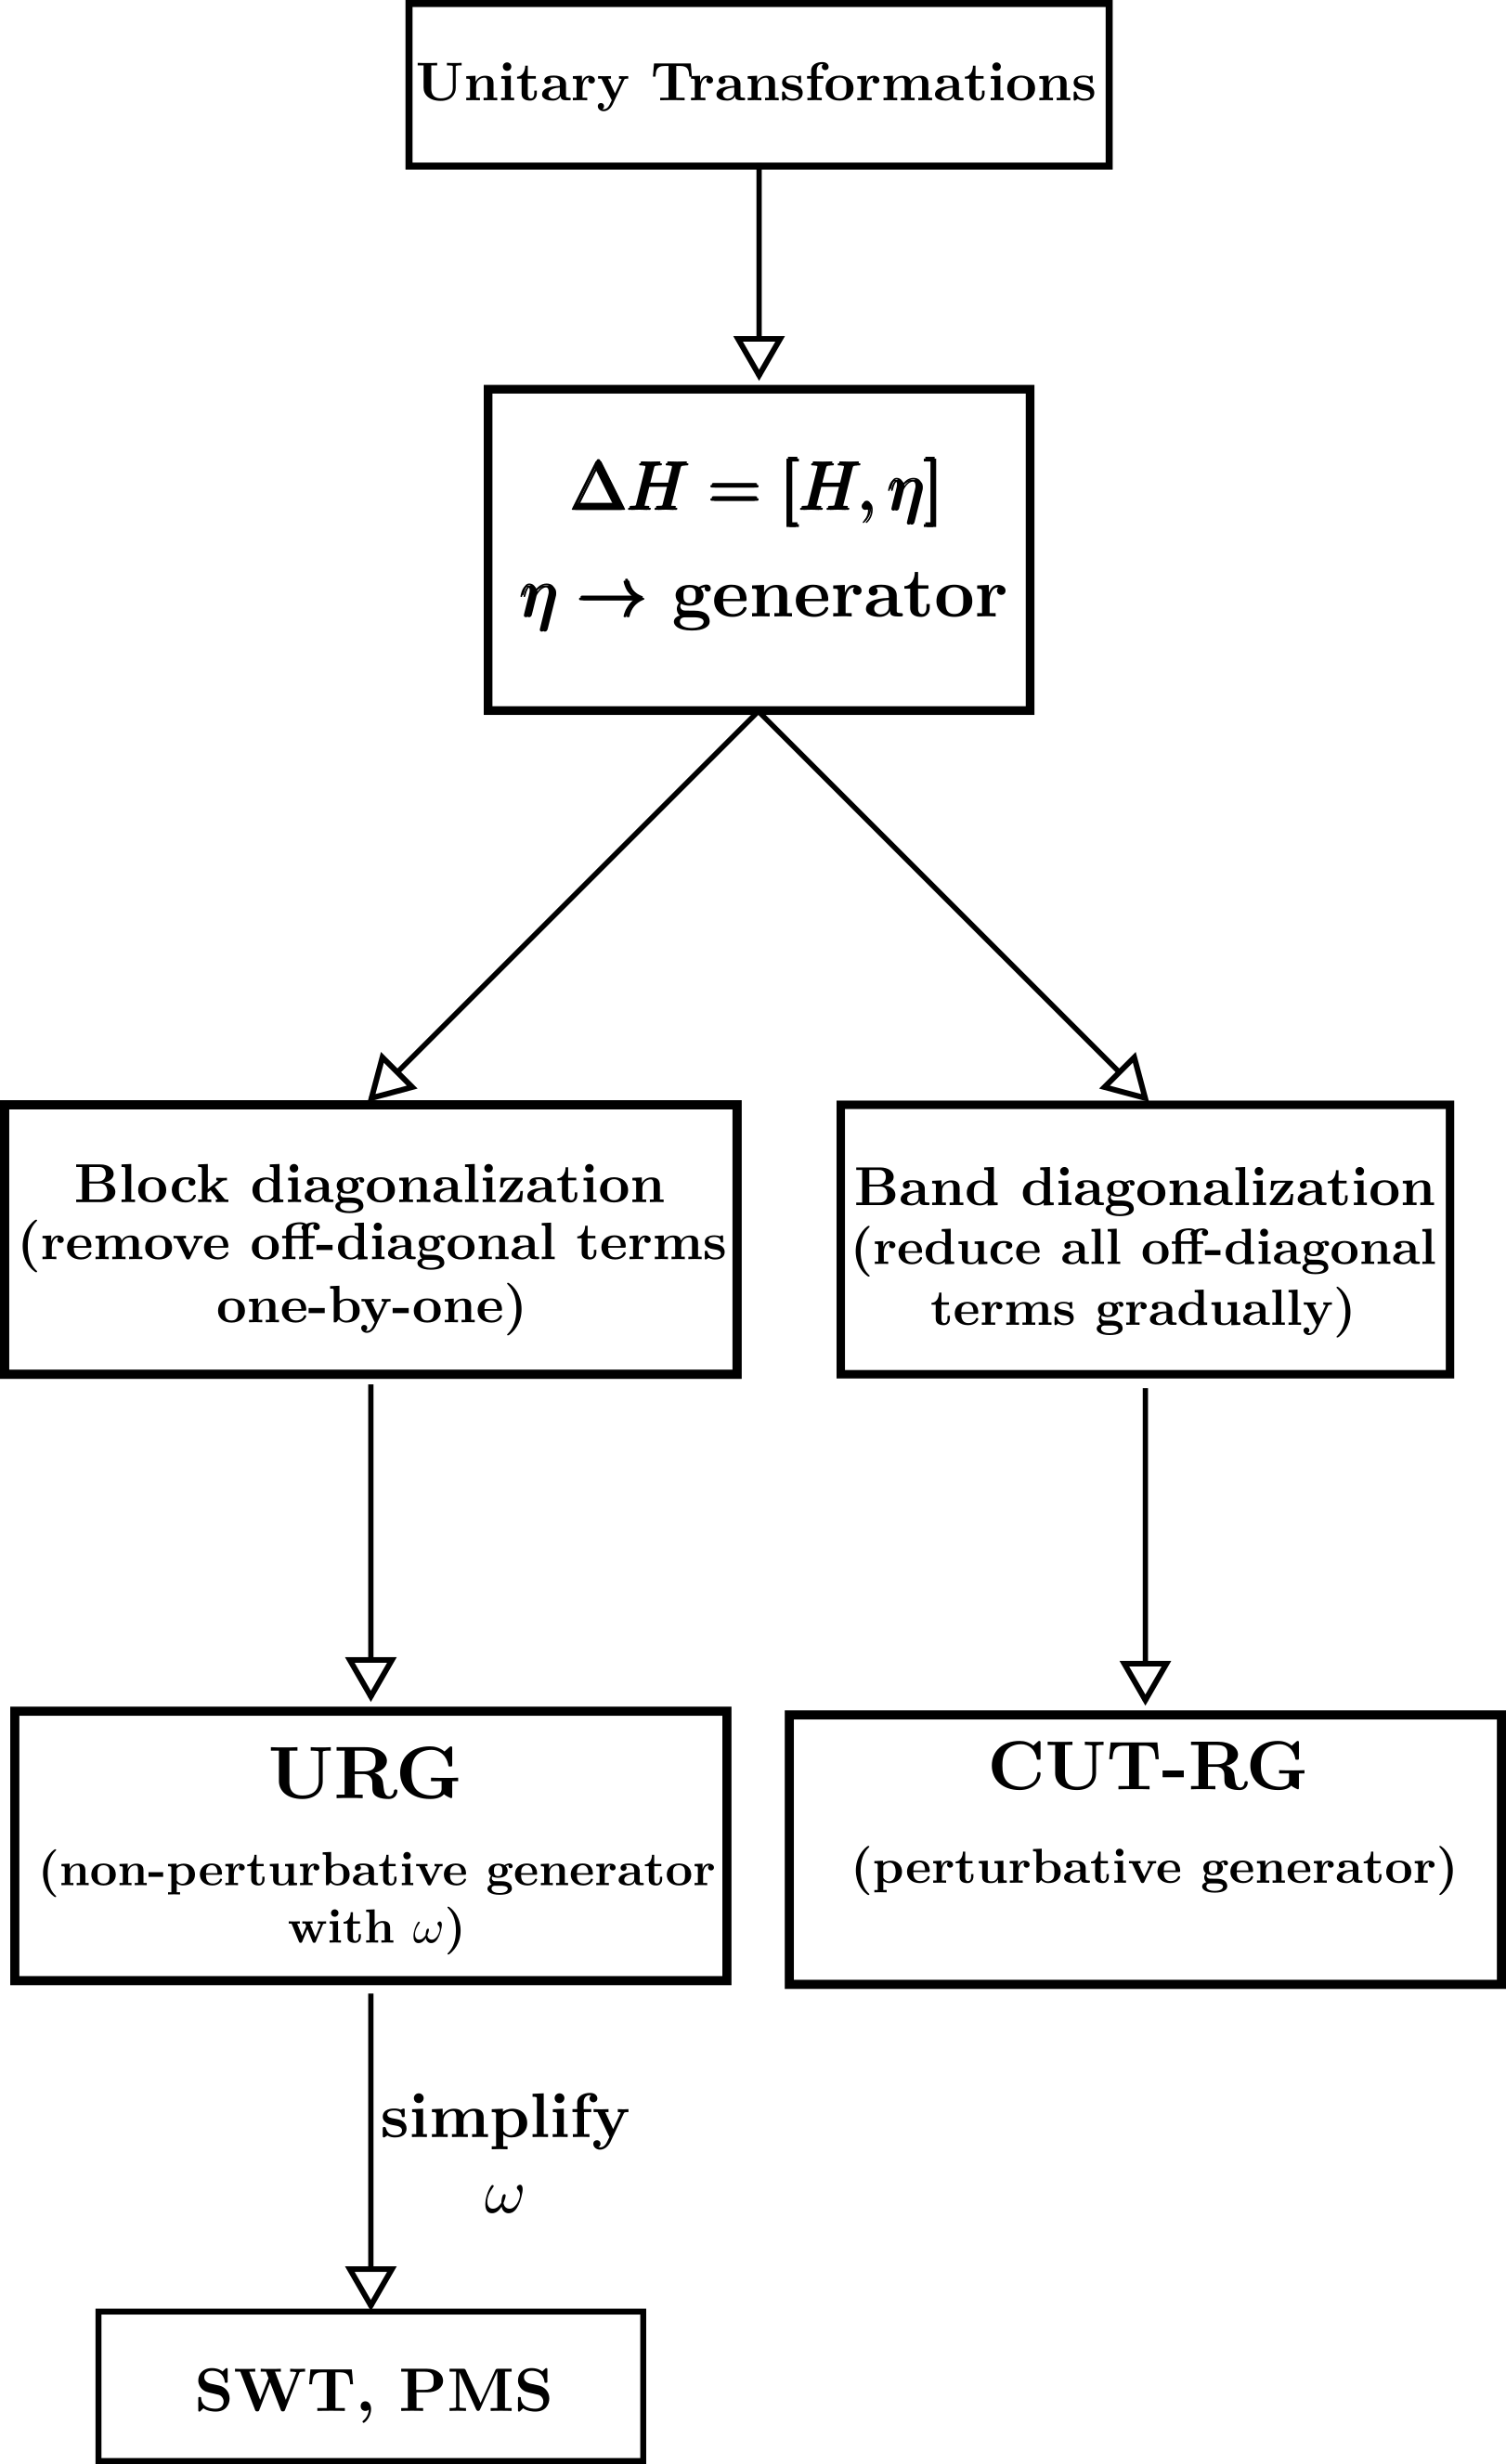
\includegraphics[scale=0.22]{../figures/unitaries.png}
	\captionof{figure}{Comparison of the various unitary transformations, depicting how each of them are related to one another.}
\end{center}
\chapter{URG of the SIAM and its Spin and Charge Generalizations}\label{siamurg}
\section{URG of the SIAM}
\subsection{Setting up the various terms in the URG}
The model is the usual single-impurity Anderson model Hamiltonian.
\begin{equation}\begin{aligned}
	\mathcal{H} = \sum_{k\sigma}\epsilon_k \hat n_{k\sigma} + \sum_{k\sigma} \left(V_{k} c^\dagger_{k\sigma} c_{d\sigma} + h.c.\right) + \epsilon_{d}\sum_\sigma  \hat n_{d\sigma} +  U \hat n_{d\uparrow} \hat n_{d\downarrow}
\end{aligned}\end{equation}
To allow the calculation of both particle and hole kinetic energies, we will write the kinetic energy part as \(\sum_{k\sigma}\epsilon_k \tau_{k\sigma}\), where \(\tau = \hat n - \frac{1}{2}\) and drop the extra constant part.
\begin{equation}
	\label{model:siam}
	\mathcal{H} = \sum_{k\sigma}\epsilon_k \tau_{k\sigma} + \sum_{k\sigma} \left(V_{k} c^\dagger_{k\sigma} c_{d\sigma} + h.c.\right) + \epsilon_{d}\sum_\sigma  \hat n_{d\sigma} +  U \hat n_{d\uparrow} \hat n_{d\downarrow}
\end{equation}
The renormalization is
\begin{equation}\begin{aligned}
\label{newh}
c^\dagger_{q\beta}T \eta + T^\dagger c_{q\beta}\eta_0^\dagger
\end{aligned}\end{equation}
We will be decoing an electron \(q\beta\) at the energy shell \(\epsilon_q\). The diagonal part (that comes down in the denominator) is
\begin{equation}\begin{aligned}
	\label{term1}
\mathcal{H}_d = \epsilon_q \tau_{q\beta} + \epsilon_{d}\sum_\sigma  \hat n_{d\sigma} +  U \hat n_{d\uparrow} \hat n_{d\downarrow}
\end{aligned}\end{equation}
Since this is the first step of the RG, the shell being decoupled is the highest one, which we call \(\Lambda_N\).
\subsection{Calculation of renormalization}
The \(\eta\) is
\begin{equation}\begin{aligned}
	\eta = \frac{1}{\hat \omega - \mathcal{H}_d}T^\dagger c_{q\beta} &= \frac{1}{\hat \omega - \epsilon_q \tau_{q\beta} - \epsilon_{d}\sum_\sigma  \hat n_{d\sigma} -  U \hat n_{d\uparrow} \hat n_{d\downarrow}}V_q^* c^\dagger_{d\beta}c_{q\beta}\\
							     &= \frac{1}{\hat \omega + \frac{1}{2}\epsilon_q - \epsilon_d - \left(\epsilon_d + U \right)\hat n_{d\overline\beta}}V_q^* c^\dagger_{d\beta}c_{q\beta}
\end{aligned}\end{equation}
We substituted \(\tau_{q\beta} = -\frac{1}{2}\) and \(\hat n_{d\beta} = 1\) because of the off-diagonal terms in the numerator.
The renormalization in the particle sector (\(\hat n_{q\beta} = \hat n_{q\overline\beta} = 1\)), at an energy \(-\epsilon_q\) is
\begin{equation}\begin{aligned}
\Delta \mathcal{H} = c^\dagger_{q\beta} T \eta= \frac{|V_q|^2}{\hat \omega - \frac{1}{2}\epsilon_q - \epsilon_d - \left(\epsilon_d + U \right)\hat n_{d\overline\beta}} \left(1 - \hat n_{d\beta}\right)\hat n_{q\beta} 
\end{aligned}\end{equation}
Similarly, the renormalization in the hole sector (\(\hat n_{q\beta} = \hat n_{q\overline\beta} = 0\)), at an energy \(\epsilon_q\) is:
\begin{equation}
	\Delta \mathcal{H} = T^\dagger c \eta_0^\dagger = \frac{|V_q|^2}{\hat \omega - \frac{1}{2}\epsilon_q - \epsilon_d\hat n_{d\overline\beta}}\left(1 - \hat n_{q\beta}\right)\hat n_{d\beta}
\end{equation}
Therefore, the total renormalization obtained from decoupling a particle state (\(\hat n_{q\beta}=1\)) at \(-\epsilon_q\) and a hole state (\(\hat n_{q\beta}=0\)) at \(\epsilon_q\) is
\begin{equation}\begin{aligned}
	\Delta \mathcal{H} &= \frac{|V_q|^2 \left(1 - \hat n_{d\beta}\right)}{\hat \omega - \frac{1}{2}\epsilon_q - \epsilon_d - \left(\epsilon_d + U \right)\hat n_{d\overline\beta}} + \frac{|V_q|^2\hat n_{d\beta}}{\hat \omega - \frac{1}{2}\epsilon_q - \epsilon_d \hat n_{d\overline\beta}}\\
		    &=|V_q|^2 \left[\frac{\left(1 - \hat n_{d\beta}\right)\hat n_{d\overline\beta}}{\omega_1 - \frac{1}{2}\epsilon_q - 2\epsilon_d - U} + \frac{\left(1 - \hat n_{d\beta}\right)\left( 1-\hat n_{d\overline\beta} \right)}{\omega_2 - \frac{1}{2}\epsilon_q - \epsilon_d} + \frac{\hat n_{d\beta} \hat n_{d\overline\beta}}{\omega_3 - \frac{1}{2}\epsilon_q - \epsilon_d} + \frac{\hat n_{d\beta}\left( 1- \hat n_{d\overline\beta}\right) }{\omega_4 - \frac{1}{2}\epsilon_q}\right]\\
\end{aligned}\end{equation}
To relate the \(\omega_i\), we look at the their values obtained by substituting the energies of the initial states:
\begin{equation}\begin{aligned}
	\omega_1 = \omega_4 &= -\frac{1}{2}\epsilon_q + \epsilon_d\\
	\omega_2 &= -\frac{1}{2}\epsilon_q\\
	\omega_3 &= -\frac{1}{2}\epsilon_q + 2\epsilon_d + U\\
\end{aligned}\end{equation}
Defining \(\omega \equiv \omega_2\) (because \(\omega_2\) has the simplest form), we can write
\begin{equation}\begin{aligned}
	\omega_1 = \omega_4 &= \omega + \epsilon_d\\
	\omega_2 &= \omega\\
	\omega_3 &= \omega + 2\epsilon_d + U\\
\end{aligned}\end{equation}
The renormalization then becomes
\begin{equation}\begin{aligned}
	\label{vanilla:siam:ren}
	\Delta \mathcal{H} = |V_q|^2 \left[\frac{\left(1 - \hat n_{d\beta}\right)\hat n_{d\overline\beta}}{\omega - \frac{1}{2}\epsilon_q - \epsilon_d - U} + \frac{\left(1 - \hat n_{d\beta}\right)\left( 1-\hat n_{d\overline\beta} \right)}{\omega - \frac{1}{2}\epsilon_q - \epsilon_d} + \frac{\hat n_{d\beta} \hat n_{d\overline\beta}}{\omega - \frac{1}{2}\epsilon_q + \epsilon_d + U} + \frac{\hat n_{d\beta}\left( 1- \hat n_{d\overline\beta}\right) }{\omega - \frac{1}{2}\epsilon_q + \epsilon_d}\right]
\end{aligned}\end{equation}
\subsection{Scaling equations}
Once we have the renormalization for decoupling one electronic or hole state, we can just sum over the spins and momenta to get the total renormalization upon decoupling the entire shells \(\pm \epsilon_q\). From the structure of \(\Delta \mathcal{H}\) in eq.~\ref{vanilla:siam:ren}, we can see that there are renormalizations to all three configuration energies of the impurity: the doublon energy \(E_2\) corresponding to the state  \(\hat n_{d\beta}\hat n_{d\overline\beta}\), the single energy \(E_1\) corresponding to (\(\hat n_{d\beta}(1 - \hat n_{d\overline\beta}) + \hat n_{d\overline\beta}(1 - \hat n_{d\beta})\), and the holon energy \(E_0\) corresponding to \((1 - \hat n_{d\beta})(1 - \hat n_{d\overline\beta}) + \hat n_{d\overline\beta}(1 - \hat n_{d\beta})\).
\begin{equation}\begin{aligned}
	\label{urg-siam}
	\Delta E_2 &= +2\sum_{q}\frac{|V_q|^2}{\omega - \frac{1}{2}\epsilon_q + \epsilon_d + U }\\
	\Delta E_1 &= +\sum_{q}\frac{|V_q|^2}{\omega - \frac{1}{2}\epsilon_q + \epsilon_d} + \sum_{q}\frac{|V_q|^2}{\omega - \frac{1}{2}\epsilon_q - \epsilon_d - U}\\
	\Delta E_0 &= +2\sum_{q}\frac{|V_q|^2}{\omega - \frac{1}{2}\epsilon_q - \epsilon_d}
\end{aligned}\end{equation}
Using the relations \(\epsilon_d = E_1 - E_0\) and \(U = E_2 + E_0 - 2E_1\), we can write
\begin{equation}\begin{aligned}
	\Delta \epsilon_d &= +\sum_{q}\frac{|V_q|^2}{\omega - \frac{1}{2}\epsilon_q + \epsilon_d} + \sum_{q}\frac{|V_q|^2}{\omega - \frac{1}{2}\epsilon_q - \epsilon_d - U} - 2\sum_{q}\frac{|V_q|^2}{\omega - \frac{1}{2}\epsilon_q - \epsilon_d}\\
	\Delta U &= \sum_{q}\frac{2|V_q|^2}{\omega - \frac{1}{2}\epsilon_q + \epsilon_d + U } + \sum_{q}\frac{2|V_q|^2}{\omega - \frac{1}{2}\epsilon_q - \epsilon_d} - \sum_{q}\frac{2|V_q|^2}{\omega - \frac{1}{2}\epsilon_q + \epsilon_d} - \sum_{q}\frac{2|V_q|^2}{\omega - \frac{1}{2}\epsilon_q - \epsilon_d - U}\\
\end{aligned}\end{equation}
\subsection{Connection to Poor Man's scaling}\label{urg2pms}
To obtain the results of Poor Man's scaling \cite{haldane}\cite{Jefferson},  we can look at various regimes. First we look at the case when both \(\epsilon_d\) and \(U\) are small such that both the singly-occupied and doubly-occupied subspaces of the impurity are comfortably inside the bandwidth, \(U,\epsilon_d \ll \epsilon_q\). We can then ignore the \(\epsilon_d\) and \(U\) in the denominator compared to the \(\epsilon_q\).
\begin{equation}\begin{aligned}
\Delta \epsilon_d &= \sum_{q}\frac{|V_q|^2}{\omega - \frac{1}{2}\epsilon_q} + \sum_{q}\frac{|V_q|^2}{\omega - \frac{1}{2}\epsilon_q} - 2\sum_{q}\frac{|V_q|^2}{\omega - \frac{1}{2}\epsilon_q}\\
\Delta U &= 2\sum_{q}\frac{|V_q|^2}{\omega - \frac{1}{2}\epsilon_q} + 2\sum_{q}\frac{|V_q|^2}{\omega - \frac{1}{2}\epsilon_q} - 2\sum_{q}\frac{|V_q|^2}{\omega - \frac{1}{2}\epsilon_q} - 2\sum_{q}\frac{|V_q|^2}{\omega - \frac{1}{2}\epsilon_q}
\end{aligned}\end{equation}
Assuming the upper and lower band edges are symmetrical such that \(\sum_{-D} = \sum_D\), we get \(\Delta \epsilon_d = \Delta U = 0\). 
\\\\In the regime \(U \gg \epsilon_q \gg \epsilon_d\), the doubly-occupied state is far above the bandwidth. We can now ignore the terms that have \(U\) in the denominator. We get
\begin{equation}\begin{aligned}
\Delta \epsilon_d &= \sum_{q}\frac{|V_q|^2}{\omega - \frac{1}{2}\epsilon_q} - 2\sum_{q}\frac{|V_q|^2}{\omega - \frac{1}{2}\epsilon_q}\\
\Delta U &= 2\sum_{q}\frac{|V_q|^2}{\omega - \frac{1}{2}\epsilon_q}  - 2\sum_{q}\frac{|V_q|^2}{\omega - \frac{1}{2}\epsilon_q} 
\end{aligned}\end{equation}
Again assuming symmetrical upper and lower edges, and isotropic dispersion \(\epsilon_q=D\) and \(\sum_q |V|^2 = \frac{\Delta}{\pi}|\delta D|\), we get
\begin{equation}\begin{aligned}
\Delta U &= 0\\
\delta \epsilon_d &= -\frac{\Delta}{\pi}\frac{1}{\omega - \frac{1}{2} D}
\end{aligned}\end{equation}
There we replaced the difference symbol \(\Delta\) with \(\delta\) to avoid confusion with the hybridisation \(\Delta \sim \sum V^2\). For low quantum fluctuations, we can ignore the renormalization in the couplings and replace \(\omega\) with the initial conduction electron energy: \(\omega = \epsilon_q\tau_{q\beta} = -\frac{1}{2} D\).
\begin{equation}\begin{aligned}
\delta \epsilon_d &= \frac{\Delta}{\pi}\frac{\delta D}{D}
\end{aligned}\end{equation}
This is the one-loop scaling equation.
\subsection{Particle-Hole symmetry}
The Anderson model Hamiltonian, eq.~\ref{andham}, has an impurity particle-hole symmetry for a certain condition of the couplings. To see this, we apply the particle-hole transformation \(c_k \to c^\dagger_k, c_d \to -c^\dagger_d\) to the Hamiltonian. Since we are looking at the impurity symmetry, we will only look at the terms involving the impurity. The particle-hole symmetry of the conduction bath is a separate thing and that requires a specific lattice. Hence we will not consider kinetic energy term in this discussion. The rest of the terms transform as
\begin{gather}
    \epsilon_d \sum_\sigma \hat n_{d\sigma} \to 2\epsilon_d - \epsilon_d \sum_\sigma \hat n_{d\sigma}\label{imp1}\\
U \hat n_{d\uparrow}\hat n_{d\downarrow} \to U \hat n_{d\uparrow}\hat n_{d\downarrow} - U\sum_\sigma \hat n_{d\sigma} + U\label{imp2}\\
\sum_{k\sigma}V(k)c^\dagger_{k\sigma}c_{d\sigma} + hc \to \sum_{k\sigma}-V(k)c_{k\sigma}c^\dagger_{d\sigma} + hc = \sum_{k\sigma}V^*(k)c^\dagger_{k\sigma}c_{d\sigma} + hc \label{hop}\\
S^z\sum_{kq}s^z_{kq} \to \left(-S^z\right)\sum_{kq}\left(-s^z_{kq}\right) = S^z\sum_{kq}s^z_{kq}\label{spin1}\\
S^{\pm}\sum_{kq}s^{\mp}_{kq} \to \left(-S^{\pm}\right)\sum_{kq}\left(-s^{\mp}_{kq}\right) = S^{\pm}\sum_{kq}s^{\mp}_{kq}\label{spin2}
\end{gather}
The transformation of the spin terms, eqs.~\ref{spin1} and \ref{spin2}, can be understood from the fact that since a spin degree of freedom can be written in terms of the number operator as \(\hat S = \hat n - \frac{1}{2}\), it must transform by flipping its sign: \(\hat S = \hat n - \frac{1}{2} \to \frac{1}{2} - \hat n = -\hat S\). The spin terms are thus invariant under the particle-hole transformation. The impurity-bath hopping term can be made symmetric by making \(V(k)\) real; then we would have, from eq.~\ref{hop},
\begin{equation}\begin{aligned}
	V(k)\left(c^\dagger_{k\sigma}c_{d\sigma} + c^\dagger_{d\sigma}c_{k\sigma}\right)\to V(k)\left(c^\dagger_{d\sigma}c_{k\sigma} + c^\dagger_{k\sigma}c_{d\sigma}\right)
\end{aligned}\end{equation}
The impurity diagonal terms, \(\epsilon_d\) and \(U\), require a specific condition. Combining eqs.~\ref{imp1} and \ref{imp2},
\begin{equation}\begin{aligned}
	\epsilon_d\hat n_{d\sigma} + U\hat n_{d\uparrow}\hat n_{d\downarrow} \to \left(-\epsilon_d - U\right)\hat n_{d\sigma} + U\hat n_{d\uparrow}\hat n_{d\downarrow}
\end{aligned}\end{equation}
We dropped some constant terms in the transformed Hamiltonian. For particle-hole symmetry, the left and right hand sides must be same. The required condition is thus 
\begin{equation}\begin{aligned}
	\label{phs}
\epsilon_d = -\epsilon_d - U \implies \epsilon_d + \frac{1}{2} U = 0
\end{aligned}\end{equation}
\begin{minipage}{260pt}
    This same condition can be obtained in a more physical way. If we consider the singly-occupied state of the impurity as the reference state, the doubly-occupied state is the particle-excitation and the vacant state is the hole excitation. The energy of this particle state is \(E_2 = 2\epsilon_d + U\) and that of the hole state is \(E_0 = 0\). Particle-hole symmetry then requires the particle and hole levels to be degenerate, which means \(E_2 = E_0\), and we recover the condition eq.~\ref{phs}.
\end{minipage}
\hspace*{15pt}\begin{minipage}{200pt}
    \centering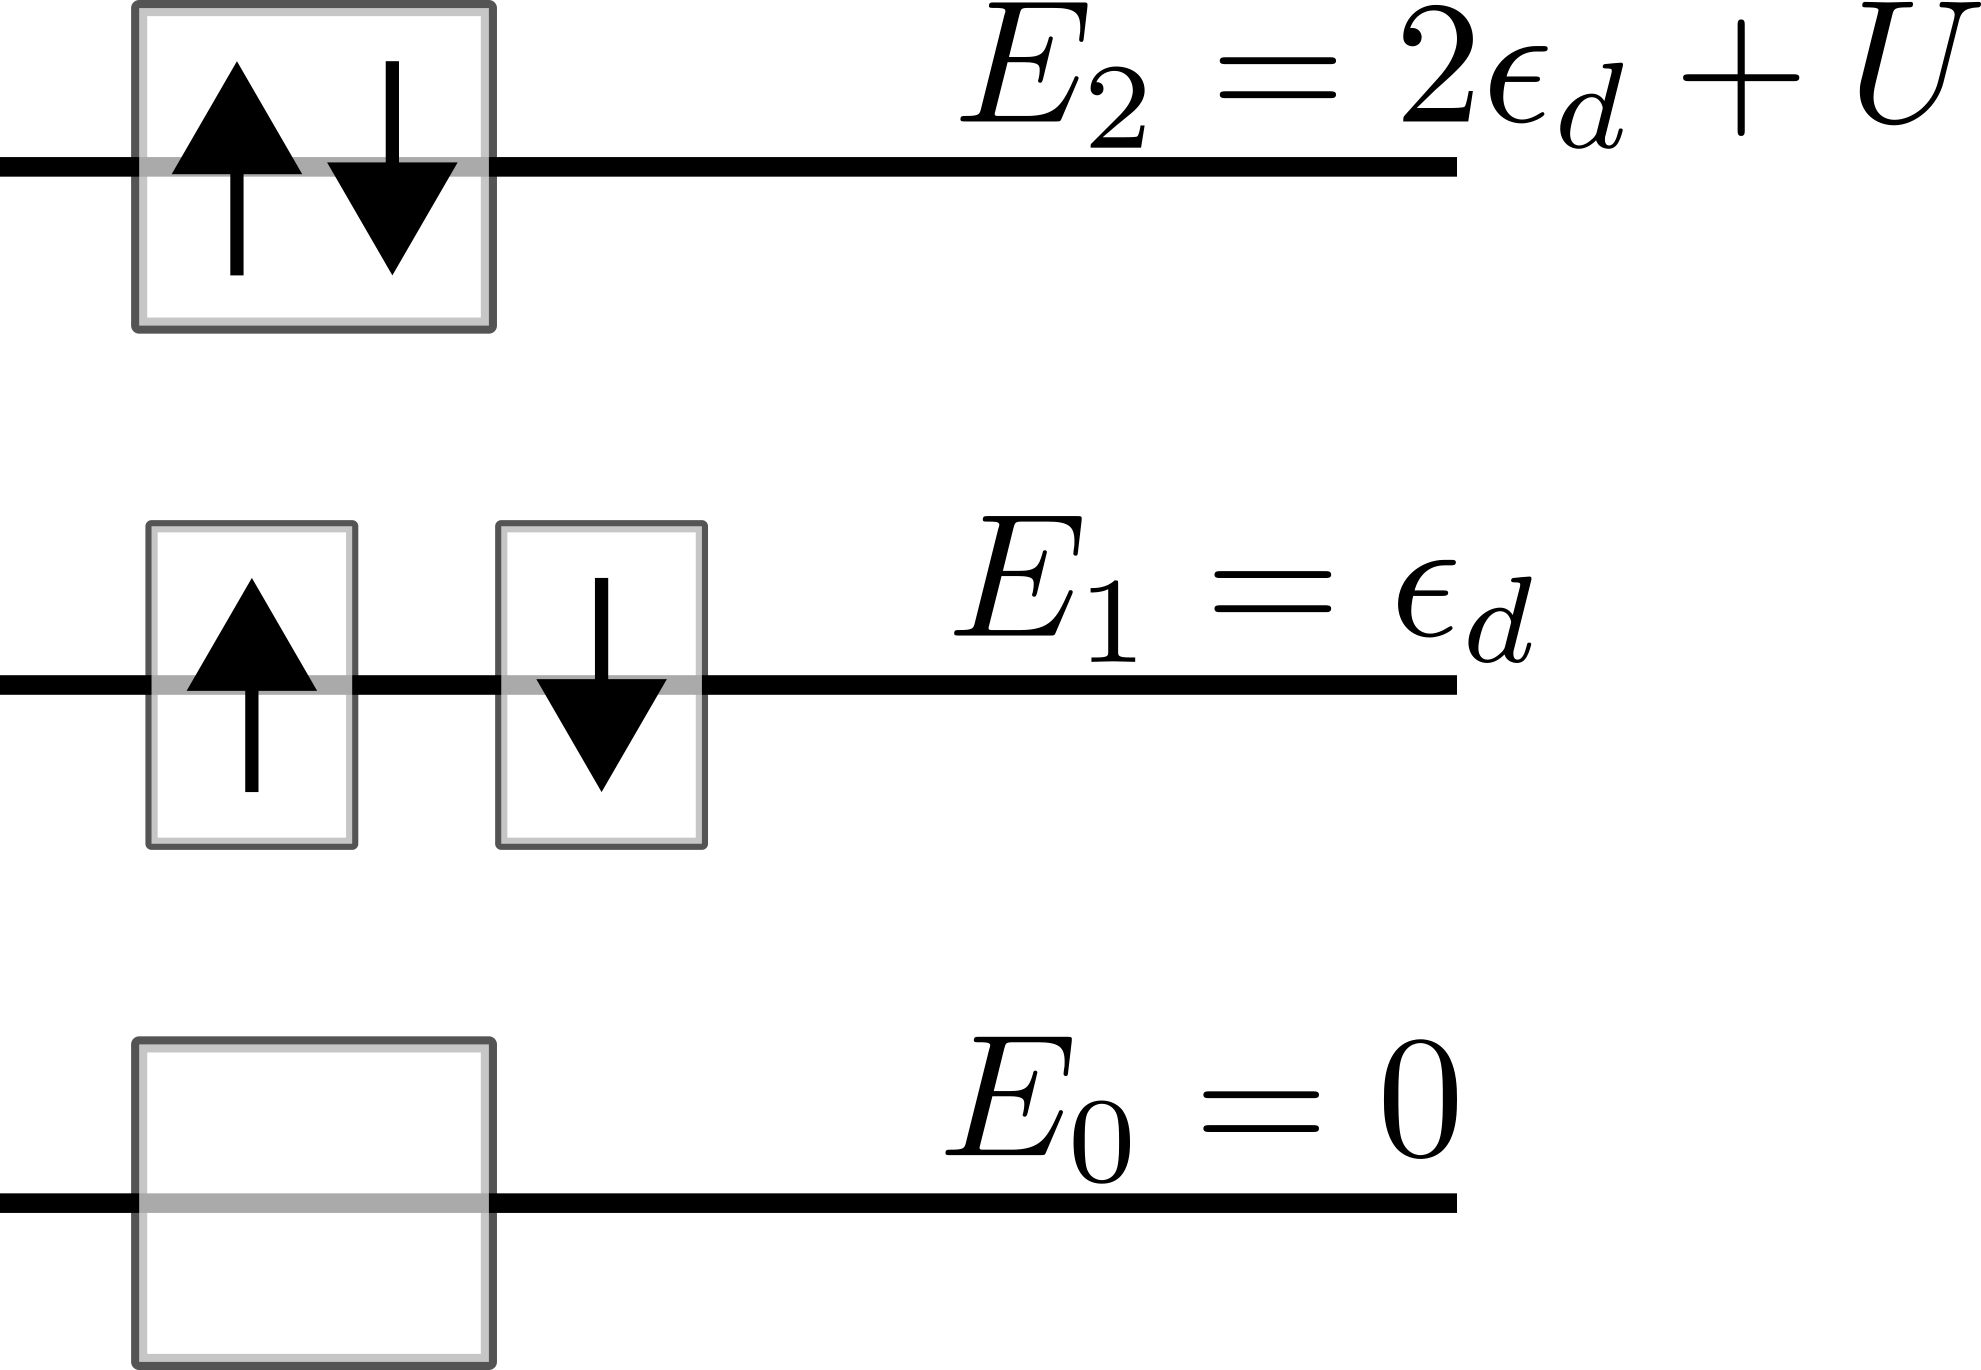
\includegraphics[scale=0.3]{phsymm.png}
    \captionof{figure}{Particle and hole excitations of the impurity}
\end{minipage}
\\\\Since the URG is unitary, if we start from a model that is particle-hole symmetric, the RG equations should uphold that symmetry. What this means is that if we have \(\epsilon_d + \frac{1}{2} U = 0\) in the bare model, the new couplings should also satisfy \(\epsilon_d^\prime + \frac{1}{2} U^\prime = 0\). This means we must have 
\begin{equation}\begin{aligned}
	\Delta\left(\epsilon_d + \frac{1}{2} U\right) = 0
\end{aligned}\end{equation}
The quantity \(\gamma = \epsilon_d + \frac{1}{2} U\) is thus an RG-invariant for the particle-hole symmetric model; it does not change under the RG flow. It is often referred to as the asymmetry parameter; it quantifies the asymmetry in the model. We need to check if our equations satisfy this. Looking at the RG equations for \(\epsilon_d\) and \(U\), we can find the RG equation for the asymmetry parameter. The slightly easier way is to just note that the renormalization in \(E_2\) should be equal to the renormalization in \(E_0\), in order for p-h symmetry to hold.
\begin{equation}\begin{aligned}
\Delta E_2 &= 2 \frac{\Delta}{\pi}\frac{1}{\omega - D + \epsilon_d + U}, \Delta E_0 &= 2 \frac{\Delta}{\pi}\frac{1}{\omega - D - \epsilon_d}
\end{aligned}\end{equation}
If we start with a particle-hole symmetric model, we will have \(-\epsilon_d = \epsilon_d + U\). Substituting that gives \(\Delta E_2= \Delta E_0\). This shows that the doublon and holon states remain equidistant from the single-particle level, thus maintaining particle-hole symmetry along the flow.
\subsection{Numerical analysis of symmetric SIAM}
We will specialize to the particle-hole symmetric case, \(2\epsilon_d + U = 0\), and a symmetric energy shell \(\epsilon_q = D\), and look at the scaling behavior of \(\epsilon_d\).
\begin{equation}\begin{aligned}
	\Delta \epsilon_d = -4|V|^2 \frac{\epsilon_d}{\left( \omega - \frac{1}{2}D \right)^2 - \epsilon_d^2}
\end{aligned}\end{equation}
Since the equation is symmetric under \(\epsilon_d \to -\epsilon_d\), we might as well work with the magnitude of the onsite energy:
\begin{equation}\begin{aligned}
	\Delta |\epsilon_d| = -4|V|^2 \frac{|\epsilon_d|}{\left( \omega - \frac{1}{2}D \right)^2 - \epsilon_d^2}
\end{aligned}\end{equation}
Depending on the signature of the denominator, the flows will be either relevant or irrelevant.
\begin{figure}[htpb]
	\centering
	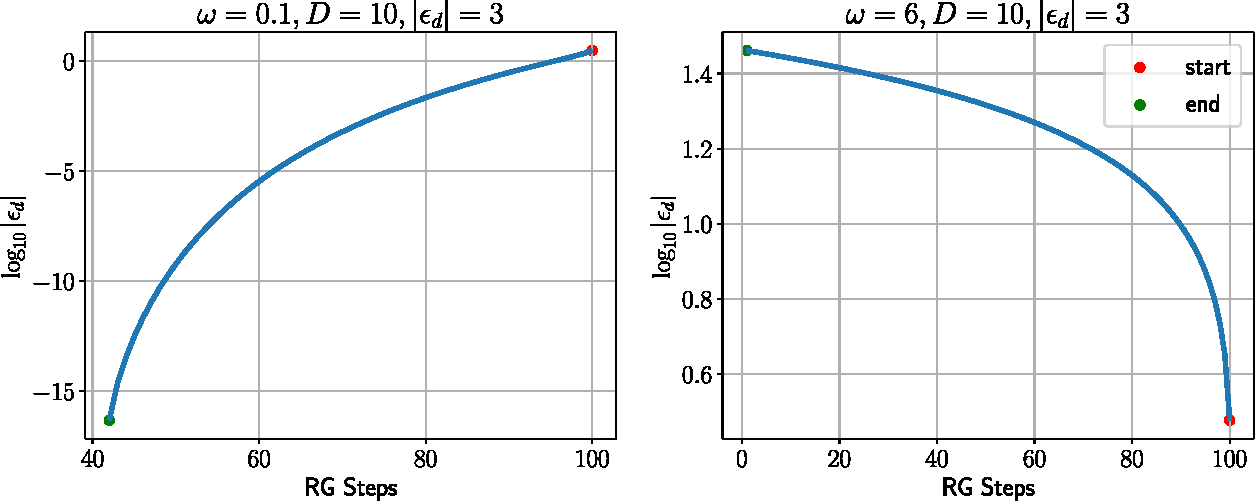
\includegraphics[width=0.99\textwidth]{../figures/ed_pure_siam.pdf}
	\caption{Left: Irrelevant flow towards \(|\epsilon_d|=0\), at low \(\omega\). Right: Relevant flow towards large \(|\epsilon_d|\), at large \(\omega\). The former can be thought of as the projection of the strong-coupling flow on to the \(\epsilon_d-D\) plane. The latter is the flow towards the local moment fixed point, if we start from a negative \(\epsilon_d\).}
\end{figure}
For the flow to the local moment fixed point, the fixed point value of \(|\epsilon_d|\) grows as we increase the bandwidth. This implies that for a thermodynamically large system, the local moment fixed point will be at \(-\epsilon_d \to \infty\). This behavior is shown in fig.~\ref{edvsD}.
\begin{figure}[htpb]
	\centering
	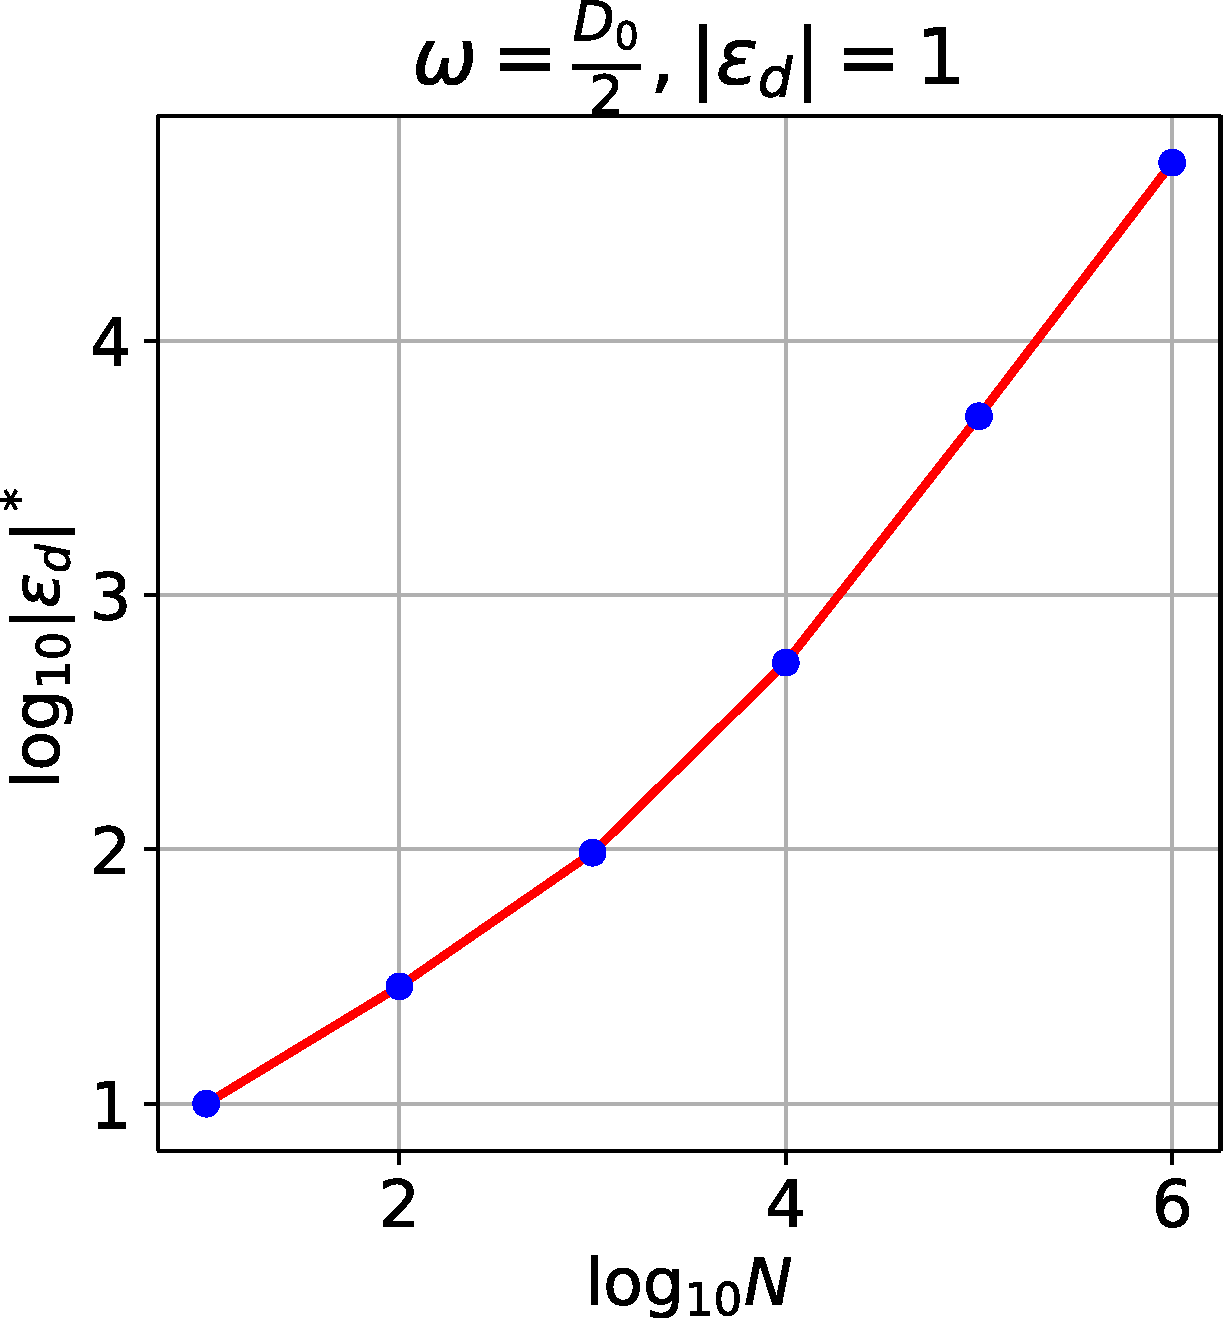
\includegraphics[width=0.6\textwidth]{../figures/ed_vs_size.pdf}
	\caption{Change in fixed point value of \(|\epsilon_d|\) with system size.}
	\label{edvsD}
\end{figure}
\section{Anderson-Kondo (spin) model URG}
In order to obtain a renormalization in \(V\), we will introduce a spin-spin interaction between the impurity and the mobile electrons. Such terms are generated when one does a Schrieffer-Wolff transformation on the SIAM, but we will find it prudent to keep these terms in the bare model itself.
\subsection{Spin-spin interaction}
We first consider a general four-Fermion interaction of the form
\begin{equation}\begin{aligned}
	\mathcal{H}_I = \sum_{k,k^\prime ,\sigma_i}u c^\dagger_{d\sigma_2}c_{d\sigma_4}c_{k^\prime \sigma_3}c^\dagger_{k\sigma_1}\delta_{\left(\sigma_1 + \sigma_2 = \sigma_3 + \sigma_4\right)}
\end{aligned}\end{equation}
The \(u\) in general depends on the spin and the momenta. Expanding the summation by using the delta gives
\begin{equation}\begin{aligned}
\mathcal{H}_I = \underbrace{\sum_{k,k^\prime ,\sigma,\sigma^\prime}u_1 \hat n_{d\sigma^\prime}c^\dagger_{k\sigma}c_{k^\prime \sigma}}_\text{spin-preserving scattering} + \overbrace{\sum_{k,k^\prime ,\sigma}u_2 c^\dagger_{d\overline\sigma}c_{d\sigma}c^\dagger_{k\sigma}c_{k^\prime \overline\sigma}}^\text{spin-flip scattering}
\end{aligned}\end{equation}
At this point, we drop the dependence of \(u\) on the momenta and assume it depends only on the spin transfer. The first term (attached with \(u_1\)) involves no spin-flip between the scattering momenta or the scattering impurity electrons (\(k\sigma \to k^\prime \sigma, d\sigma^\prime \to d\sigma^\prime\)). We label this coupling as \(u_P\). The other coupling involves a spin-flip scattering, so we label that as \(u_A\).
\begin{equation}\begin{aligned}
\mathcal{H}_{I,N} = \sum_{k,k^\prime ,\sigma,\sigma^\prime}u_P \hat n_{d\sigma^\prime}c^\dagger_{k\sigma}c_{k^\prime\sigma}+ \sum_{k,k^\prime ,\sigma}u_A c^\dagger_{d\overline\sigma}c_{d\sigma}c^\dagger_{k\sigma}c_{k^\prime \overline\sigma}
\end{aligned}\end{equation}
where the \(N\) in the denominator means the sum is over all momenta up to \(|k| = \Lambda_N\). The parallel scattering has two components, when expanded, is of the form
\begin{equation}\begin{aligned}
u_{\uparrow\uparrow}\hat n_{d\uparrow}c^\dagger_{k\uparrow}c_{k^\prime\uparrow} + u_{\downarrow\downarrow}\hat n_{d\downarrow}c^\dagger_{k\downarrow}c_{k^\prime\uparrow} + u_{\uparrow\downarrow}\hat n_{d\uparrow}c^\dagger_{k\downarrow}c_{k^\prime\downarrow} + u_{\downarrow\uparrow}\hat n_{d\downarrow}c^\dagger_{k\uparrow}c_{k^\prime\uparrow}
\end{aligned}\end{equation}
We define \(J_z\) and \(J_t\) such that this term can be written as
\begin{equation}\begin{aligned}
	\mathcal{H}_{I} &= J_z \frac{\hat n_{d\uparrow} - \hat n_{d\downarrow}}{2}\sum_{kk^\prime}\left(c^\dagger_{k\uparrow}c_{k^\prime\uparrow} - c^\dagger_{k\downarrow}c_{k^\prime\downarrow}\right) + J_t \sum_{kk^\prime}\left[ c^\dagger_{d\uparrow}c_{d\downarrow}c^\dagger_{k\downarrow}c_{k^\prime\uparrow} + c^\dagger_{d\downarrow}c_{d\uparrow}c^\dagger_{k\uparrow}c_{k^\prime\downarrow}\right]\\
			&= 2J_z S_d^z s^z + J_t \left(S_d^+ s^- + S_d^- s^+\right)
\end{aligned}\end{equation}
The spin-like operators are defined as
\begin{equation}\begin{aligned}
	S^z_d &\equiv \frac{1}{2}\left(\hat n_{d\uparrow} - \hat n_{d\downarrow}\right) \quad&S^+_d &\equiv c^\dagger_{d\uparrow}c_{d\downarrow}\quad &S^-_d \equiv c^\dagger_{d\downarrow}c_{d\uparrow}\\
	s^z_{kk^\prime} &\equiv \frac{1}{2}\left(c^\dagger_{k\uparrow}c_{k^\prime\uparrow} - c^\dagger_{k\downarrow}c_{k^\prime\downarrow}\right) \quad &s^+_{kk^\prime} &\equiv c^\dagger_{k\uparrow}c_{k^\prime\downarrow}\quad &s^-_{kk^\prime} \equiv c^\dagger_{k\downarrow}c_{k^\prime\uparrow}\\
        &&s^a \equiv \sum_{kk^\prime}s^a_{kk^\prime}
\end{aligned}\end{equation}
This is the same interaction that constitutes the Kondo model and gives rise to the quenching of the local moment at low energies. The total Hamiltonian for this \textit{Anderson-Kondo model} is thus
\begin{equation}\begin{aligned}
	\label{andham}
	\mathcal{H} = \sum_{k\sigma}\left(\epsilon_k \hat n_{k\sigma} + V_{k} c^\dagger_{k\sigma} c_{d\sigma} + h.c.\right) + \epsilon_{d}\sum_\sigma  \hat n_{d\sigma} +  U \hat n_{d\uparrow} \hat n_{d\downarrow} + 2J_z S_d^z s^z + J_t \left(S_d^+ s^- + S_d^- s^+\right)
\end{aligned}\end{equation}
For the special case of \(2J_z = 2J_t = J\), we get the SU(2) symmetric Heisenberg-like interaction
\begin{equation}\begin{aligned}
	\mathcal{H}_{I} = J \left[S^z_d s^z + \frac{1}{2}\left(S^+_d s^- + S^-_d s^+\right)\right] = J \mathbf{S_d} \cdot \mathbf{s}
\end{aligned}\end{equation}
For the URG, we take two electrons on the shell \(\Lambda_N\), \(q\beta\) and \(q\overline\beta\), then decouple the electron \(q\beta\). The reason for taking two electrons is to allow the symmetries to be preserved. For simplicity, we will only consider those diagonal terms in the denominator that either have both \(q\beta\) and \(q\overline\beta\) or  both \(q\beta\) and \(d\) or both \(q\overline\beta\) and \(d\). Terms that have purely \(q\overline\beta\) will not be considered. Also, the scattering between just \(d\) and \(q\overline\beta\) can be ignored since it is diagonal in \(q\beta\). The Hamiltonian for such a system is
\begin{equation}\begin{aligned}
\mathcal{H}_N &= H_{N-1} + H_\text{imp} + \epsilon_q\hat n_{q\beta} + 2J_z S^z_d s^z_q + V_q c^\dagger_{q\beta}c_{d\beta} + \text{h.c.} +\\
	      & \sum_{k<\Lambda_N}\left[J_z S^z_d \beta \left(c^\dagger_{k\beta}c_{q\beta} + c^\dagger_{q\beta}c_{k\beta}\right) + J_t \left(c^\dagger_{d\beta}c_{d\overline\beta}c^\dagger_{k\overline\beta}c_{q \beta} + c^\dagger_{d\overline\beta}c_{d\beta}c^\dagger_{q\beta}c_{k\overline\beta}\right)\right]\\
	      & + J_t \left(c^\dagger_{d\beta}c_{d\overline\beta}c^\dagger_{q\overline\beta}c_{q \beta} + c^\dagger_{d\overline\beta}c_{d\beta}c^\dagger_{q\beta}c_{q\overline\beta}\right)
\end{aligned}\end{equation}
where \(s_q^z = \frac{1}{2}\left(\hat n_{q\uparrow} - \hat n_{q\downarrow}\right)\) and \(H_{imp}\) is the impurity-diagonal part of the Hamiltonian (\(\epsilon_d \hat n_d + U\hat n_{d\uparrow}\hat n_{d\downarrow}\)) and 
\begin{equation}\begin{aligned}
	H_{N-1} = \sum_{k<\Lambda_N,\sigma}\left[\left(\epsilon_k +  \sigma J_z S^z_d\right)\hat n_{k\sigma} + V_k c^\dagger_{k\sigma}c_{d\sigma} + \text{h.c.}\right] + H_{I,N-1}
\end{aligned}\end{equation}
The diagonal (number-preserving) part is
\begin{equation}\begin{aligned}
	\mathcal{H}_D = H^D_{N-1} + \epsilon_q\left(\hat n_{q\beta} + \hat n_{q\overline\beta}\right) + 2J_z S^z_ds^z_{q} + H_{imp}\\
\end{aligned}\end{equation}
In line with the simplifications mentioned above, we will work with the following terms:
\begin{equation}\begin{aligned}
	\label{diag}
\mathcal{H}_D = \epsilon_q \hat n_{q\beta} + 2J_z S^z_d s^z_q + H_{imp}
\end{aligned}\end{equation}
 To allow the calculation of hole and particle energies on an equal footing, we will make a transformation at the bare model itself:
 \begin{equation}\begin{aligned}
\sum_{k\sigma} \epsilon_k \hat n_{k\sigma} &= \sum_{k\sigma} \epsilon_k \hat \tau_{k\sigma} + \mathcal{C}\\
\end{aligned}\end{equation}
where \(\tau \equiv \hat n - \frac{1}{2}\) and \(\mathcal{C}\) is non-dynamic and will hence be dropped. This transforms the diagonal part \(\mathcal{H}^D\). Eq.~\ref{diag} becomes
\begin{equation}\begin{aligned}
\mathcal{H}_D = \epsilon_q \tau_{q\beta} + 2J_z S^z_d s^z_q  + H_{imp}\\
\end{aligned}\end{equation}
The entire off-diagonal piece can be split into 6 parts:
\begin{equation}\begin{aligned}
	\mathcal{H}_X &= \underbrace{V_1^* c^\dagger_{d\beta}c_{q\beta}\hat n_{d\overline\beta}}_{T^\dagger_1 c_{q\beta}} + \overbrace{V_0^* c^\dagger_{d\beta}c_{q\beta}\left(1 - \hat n_{d\overline\beta}\right)}^{T^\dagger_2 c_{q\beta}} + \underbrace{\sum_{k<\Lambda_N}J^z_0 \hat n_{d\beta}\left(1 - \hat n_{d\overline\beta}\right) c^\dagger_{k\beta}c_{q\beta}}_{T^\dagger_3 c_{q\beta}} \\
	       &- \overbrace{\sum_{k<\Lambda_N}J^z_1 \hat n_{d\overline\beta}\left(1 - \hat n_{d\beta}\right) c^\dagger_{k\beta}c_{q\beta}}^{T^\dagger_4 c_{q\beta}} + \underbrace{\sum_{k<\Lambda_N}J^t c^\dagger_{d\beta}c_{d\overline\beta}c^\dagger_{k\overline\beta}c_{q \beta}}_{T^\dagger_5 c_{q\beta}} + \overbrace{J^t c^\dagger_{d\beta}c_{d\overline\beta}c^\dagger_{q\overline\beta}c_{q \beta}}^{T^\dagger_6 c_{q\beta}} + \text{h.c.}
\end{aligned}\end{equation}
The various parts of the off-diagonal piece are
\begin{equation}\begin{aligned}
	T_1 &= V_1 c_{d\beta}\hat n_{d\overline\beta}\\
	T_2 &= V_0 c_{d\beta}\left(1 - \hat n_{d\overline\beta}\right)\\
	T_3 &= \sum_{k<\Lambda_N}J^z_0 \hat n_{d\beta}\left(1 - \hat n_{d\overline\beta}\right) c_{k\beta}\\
	T_4 &= -\sum_{k<\Lambda_N}J^z_1 \hat n_{d\overline\beta}\left(1 - \hat n_{d\beta}\right) c_{k\beta}\\
	T_5 &= \sum_{k<\Lambda_N}J^t c^\dagger_{d\overline\beta}c_{d\beta}c_{k\overline\beta}
\end{aligned}\end{equation}
\subsection{Calculation of renormalization in particle sector}
We will first look at the renormalization of \(\epsilon_d\), \(U\) and the interaction couplings for the lower shell electrons, so we can ignore \(T_6\) for the time-being. The renormalization in the particle sector (\(\hat n_{q\beta}=1\)) is of the form
\begin{equation}\begin{aligned}
	c^\dagger_{q\beta}T \eta
\end{aligned}\end{equation}
Since we have \(\hat n_{q\beta}=1\) in the initial state, this will be at energy \(-\epsilon_q\). The generator \(\eta\) will have five parts:
\begin{equation}
	\eta = \sum_{i=1}^5\frac{1}{\omega_i - E_i^0}T^\dagger_i c_{q\beta}
\end{equation}
We need to compute a quantity of the form
\begin{flalign*}
	&\sum_{ij} \left(\frac{1}{\omega_i - E^0_i} + \frac{1}{\omega - E^0_j}\right) T_i T_j^\dagger\\ 
	&=\frac{1}{\omega_1 - E^0_1}T_1 T_1^\dagger + \frac{1}{\omega_2 - E^0_2}T_2 T_2^\dagger+\frac{1}{\omega_3 - E^0_3}T_3 T_3^\dagger+\frac{1}{\omega_4 - E^0_4}T_4 T_4^\dagger+\frac{1}{\omega_5 - E^0_5}T_5 T_5^\dagger \\
	&+\left(\frac{1}{\omega_2 - E^0_2} + \frac{1}{\omega_5 - E^0_5}\right)\left(T_2 T_5^\dagger + T_5 T_2^\dagger \right) +\left(\frac{1}{\omega_2 - E^0_2} + \frac{1}{\omega_3 - E^0_3}\right)\left(T_2 T_3^\dagger + T_3 T_2^\dagger \right) \\
	&+\left(\frac{1}{\omega_3 - E^0_3} + \frac{1}{\omega_5 - E^0_5}\right)\left(T_3 T_5^\dagger + T_5 T_3^\dagger \right)
\end{flalign*}
The diagonal parts \(E_i^0\) are
\begin{equation}\begin{aligned}
	E^0_1 &= \frac{\epsilon_q}{2} + 2\epsilon_d + U\\
	E^0_2 = E^0_5 = E^0_4 &= \frac{\epsilon_q}{2} + \epsilon_d - \frac{J_z}{2}\\
	E^0_3 &= \frac{\epsilon_q}{2} + \epsilon_d + \frac{J_z}{2}\\
\end{aligned}\end{equation}
Note that in writing these diagonal parts, we have considered the effect of \(c^\dagger_k\) on the \(J_z\) part. For example, if there is a \(\hat n_{d\beta}\left(1 - \hat n_{d\overline\beta}\right)c^\dagger_{k\beta}\) in front of the propagator, that means the intermediate state has \(\hat n_{d\beta} - \hat n_{d\overline\beta} = 1 = \hat n_{k\beta}\) and that will contribute a term \(\frac{J_z}{2} \left(\hat n_{d\beta} - \hat n_{d\overline\beta}\right)\hat n_{k\beta} = \frac{J_z}{2}\) to \(E^0\). Also, while calculating \(E_5\), we have ignored the presence of \(\hat n_{q\overline\beta}\), because it violates the spin reversal symmetry for this term.
\\\\Defining \(\xi_i \equiv \omega_i - E_i^0\) and evaluating the terms \(T_i T_j^\dagger\) gives
\begin{equation}\begin{aligned}
	&\sum_{ij} \left(\frac{1}{\omega_i - E^0_i} + \frac{1}{\omega - E^0_j}\right) T_i T_j^\dagger\\ 
	&=\frac{|V_1|^2}{\xi_1}\left( 1 - \hat n_{d\beta} \right) \hat n_{d\overline\beta} + \frac{|V_0|^2}{\xi_2}\left( 1 - \hat n_{d\beta} \right) \left( 1 - \hat n_{d\overline\beta} \right) \\
	&+ \frac{1}{4}\left[ {J_0^z}^2\frac{\hat n_{d\beta}\left( 1 - \hat n_{d\overline\beta} \right) }{\xi_3} + {J_1^z}^2\frac{\hat n_{d\overline\beta}\left( 1 - \hat n_{d\beta} \right)}{\xi_4} \right]c_{k^\prime\beta}c^\dagger_{k\beta} + \frac{1}{\xi_5}J_t^2 \left( 1 - \hat n_{d\beta} \right) \hat n_{d\overline\beta} c_{k^\prime\overline\beta}c^\dagger_{k\overline\beta} \\
	&- \frac{1}{2} \left(\frac{1}{\xi_2} + \frac{1}{\xi_5}\right)J_t\left( 1 - \hat n_{d\beta}\right) \left(V_0 c^\dagger_{k\overline\beta}c_{d\overline\beta} + \text{h.c.}\right) - \frac{1}{2}\left(\frac{1}{\xi_2} + \frac{1}{\xi_3}\right)\frac{J^z_0}{2}\left(1 - \hat n_{d\overline\beta}\right)\left(V_0 c^\dagger_{k\beta}c_{d\beta} + \text{h.c.}\right) \\
	&-\frac{1}{2}\left(\frac{1}{\xi_3} + \frac{1}{\xi_5}\right)\frac{J_t J^z_0}{2}\left(c^\dagger_{d\beta}c_{d\overline\beta}c^\dagger_{k\overline\beta}c_{k^\prime\beta} + \text{h.c.}\right)
\end{aligned}\end{equation}
The indices \(k\) and \(k^\prime\) are being summed over, wherever they appear.
\subsection{Calculation of renormalization in hole sector}
The renormalization in the particle sector (\(\hat n_{q\beta}=0\)) is of the form
\begin{equation}\begin{aligned}
	T^\dagger_{q\beta}c \eta_0^\dagger
\end{aligned}\end{equation}
where \(\eta_0^\dagger\) is of the form
\begin{equation}
	\eta_0^\dagger = \sum_{i=1}^5\frac{1}{\omega^\prime_i - E_i^1}c^\dagger_{q\beta} T_i
\end{equation}
This will be at an energy \(+\epsilon_q\), because the state is occupied. The scattering terms \(T_i\) are already written down in the previous subsection. The diagonal parts are
\begin{equation}\begin{aligned}
	E^1_1 = E^1_4 = E^1_5 &= \frac{\epsilon_q}{2} + \epsilon_d - \frac{J_z}{2}\\
	E^1_2 &= \frac{\epsilon_q}{2}\\
	E^1_3 &= \frac{\epsilon_q}{2} + \epsilon_d + \frac{J_z}{2} \\
\end{aligned}\end{equation}

The renormalization can be computed by calculating \(\sum_{ij} T_i^\dagger T_j\).
\begin{flalign*}
	&\sum_{ij} \left(\frac{1}{\omega^\prime_i - E^1_i} + \frac{1}{\omega^\prime - E^1_j}\right) T_i^\dagger T_j\\ 
	&=\frac{|V_1|^2}{\xi^\prime_1}\hat n_{d\overline\beta}\hat n_{d\beta} + \frac{|V_0|^2}{\xi^\prime_2}\hat n_{d\beta}\left(1 - \hat n_{d\overline\beta}\right)\\
	&+\frac{1}{4}\left[ {J_0^z}^2\frac{\hat n_{d\beta}\left( 1 - \hat n_{d\overline\beta} \right) }{\xi^\prime_3} + {J_1^z}^2\frac{\hat n_{d\overline\beta}\left( 1 - \hat n_{d\beta} \right)}{\xi^\prime_4} \right]c^\dagger_{k\beta}c_{k^\prime\beta} + \frac{1}{\xi^\prime_5}J_t^2 \left( 1 - \hat n_{d\overline\beta} \right) \hat n_{d\beta} c^\dagger_{k\overline\beta} c_{k^\prime\overline\beta}\\
	&-\frac{1}{2} \left(\frac{1}{\xi^\prime_4} + \frac{1}{\xi^\prime_1}\right)\frac{J_1^z}{2}\hat n_{d\overline\beta} \left(V_1 c^\dagger_{k\beta}c_{d\beta} + \text{h.c.}\right) - \frac{1}{2}\left(\frac{1}{\xi^\prime_1} + \frac{1}{\xi^\prime_5}\right)J_t \hat n_{d\beta}\left(V_1 c^\dagger_{k\overline\beta}c_{d\overline\beta} + \text{h.c.}\right)\\
	&-\frac{1}{2}\left(\frac{1}{\xi^\prime_4} + \frac{1}{\xi^\prime_5}\right)\frac{J_t J^z_1}{2}\left(c^\dagger_{d\beta}c_{d\overline\beta}c^\dagger_{k\overline\beta}c_{k^\prime\beta} + \text{h.c.}\right) 
\end{flalign*}
where \(\xi^\prime_i\) is defined similar to the particle sector: \(\xi^\prime_i = \omega_i^\prime - E_i^1\). The indices \(k\) and \(k^\prime\) are being summed over, wherever they appear.
\subsection{Relating the \(\omega_i\) and \(\omega_i^\prime\)}
To relate the \(\omega_i\) and their primed counterparts, we will look at their bare non-interacting values:
\begin{equation}\begin{aligned}
	\omega_1 &= -\frac{1}{2}\epsilon_q + \epsilon_d \\
	\omega_2 &= -\frac{1}{2}\epsilon_q\\
	\omega_3 &= -\frac{1}{2}\epsilon_q + \epsilon_d + \frac{J_z}{2}\\
	\omega_5 = \omega_4 &= -\frac{1}{2}\epsilon_q + \epsilon_d - \frac{J_z}{2}\\
\end{aligned}\end{equation}
We will \textit{assume} that the relations between these values of \(\omega_i\) will hold for the URG \(\omega_i\) along the flow as well. We want to write all the \(\omega_i\) in terms of a single \(\omega = -\frac{\epsilon_q}{2} - \frac{1}{2}J_z\). %-\frac{\epsilon_q}{2} - \frac{1}{2}J_z\).
\begin{equation}\begin{aligned}
	\omega_1 &= \omega + \frac{J_z}{2} + \epsilon_d \\
	\omega_2 &= \omega + \frac{J_z}{2}\\
	\omega_3 &= \omega + J_z+ \epsilon_d \\
	\omega_5 = \omega_4 &= \omega+ \epsilon_d 
\end{aligned}\end{equation}
The denominators can now be written in terms of the single \(\omega\):
\begin{equation}\begin{aligned}
	\xi_1 &= \omega - \frac{\epsilon_q}{2} - \epsilon_d - U + \frac{J_z}{2}\\
	\xi_2 &= \omega - \frac{\epsilon_q}{2} - \epsilon_d + J_z\\
	\xi_3 = \xi_4 = \xi_5 &= \omega - \frac{\epsilon_q}{2} + \frac{J_z}{2}\\
\end{aligned}\end{equation}
Similarly, for the \(\omega_i^\prime\) of the hole sector, we have
\begin{equation}\begin{aligned}
	\omega^\prime_1 &= -\frac{1}{2}\epsilon_q + 2\epsilon_d + U\\
	\omega^\prime_2 &= -\frac{1}{2}\epsilon_q + \epsilon_d\\
	\omega^\prime_3 &= -\frac{1}{2}\epsilon_q + \epsilon_d + \frac{J_z}{2}\\
	\omega^\prime_4 = \omega^\prime_5 &= -\frac{1}{2}\epsilon_q + \epsilon_d - \frac{J_z}{2}\\
\end{aligned}\end{equation}
Writing these in terms of \(\omega = -\frac{\epsilon_q}{2} - \frac{1}{2}J_z\) gives
\begin{equation}\begin{aligned}
	\omega^\prime_1 &= \omega + U + \frac{J_z}{2}\\
	\omega^\prime_2 &= \omega + \epsilon_d + \frac{J_z}{2}\\
	\omega^\prime_3 &= \omega + \epsilon_d + J_z\\
	\omega^\prime_4 &= \omega^\prime_5 = \omega + \epsilon_d 
\end{aligned}\end{equation}
The denominators are therefore
\begin{equation}\begin{aligned}
	\xi_1^\prime &= \omega - \frac{\epsilon_q}{2} + \epsilon_d + U + J_z\\
	\xi_2^\prime &= \omega - \frac{\epsilon_q}{2} + \epsilon_d + \frac{J_z}{2}\\
	\xi_3^\prime = \xi_4^\prime = \xi_5^\prime &= \omega - \frac{\epsilon_q}{2} + \frac{J_z}{2} = \xi_3 = \xi_4 = \xi_5\\
\end{aligned}\end{equation}
\subsection{Making sense of the various terms}
We will now look at each of the renormalizations separately. Note that the indices \(k\) and \(k^\prime\) are being summed over, wherever they appear. The first two terms in each sector form a part of the renormalization in \(\epsilon_d\) and \(U\).
\begin{equation}\begin{aligned}
\frac{|V_1|^2}{\xi_1}\left( 1 - \hat n_{d\beta} \right) \hat n_{d\overline\beta} + \frac{|V_0|^2}{\xi_2}\left( 1 - \hat n_{d\beta} \right) \left( 1 - \hat n_{d\overline\beta} \right) + \frac{|V_1|^2}{\xi^\prime_1}\hat n_{d\overline\beta}\hat n_{d\beta} + \frac{|V_0|^2}{\xi^\prime_2}\hat n_{d\beta}\left(1 - \hat n_{d\overline\beta}\right)
\end{aligned}\end{equation}
We can read off the renormalizations in the doublon, spin and holon states. Note that the spin (\(\hat n_{d}=1\)) are only renormalizedby half, because the other half of the renormalization comes when you decouple the other spin \(\overline\beta\).
\begin{equation}\begin{aligned}
	\Delta E_2 = \frac{|V_1|^2}{\xi^\prime_1}, && \Delta E_1 =\frac{|V_1|^2}{2\xi_1} + \frac{|V_0|^2}{2\xi_2^\prime}, && \Delta E_0 = \frac{|V_0|^2}{\xi_2}
\end{aligned}\end{equation}
Using \(\epsilon_d = E_1 - E_0\) and \(U = E_2 + E_0 - 2E_1\), we can write
\begin{equation}\begin{aligned}
	\label{edU}
	\Delta \epsilon_d &= \frac{|V_1|^2}{2\xi_1} + \frac{|V_0|^2}{2\xi_2^\prime} - \frac{|V_0|^2}{\xi_2}\\
	\Delta U &= \frac{|V_1|^2}{\xi_1^\prime} + \frac{|V_0|^2}{\xi_2} - \frac{|V_1|^2}{\xi_1} - \frac{|V_0|^2}{\xi_2^\prime}
\end{aligned}\end{equation}
The \(J_z^2\) terms, together, give
\begin{equation}\begin{aligned}
\frac{J_z^2}{4}\left[\frac{\hat n_{d\beta}\left( 1 - \hat n_{d\overline\beta} \right) }{\xi_3} + \frac{\hat n_{d\overline\beta}\left( 1 - \hat n_{d\beta} \right)}{\xi_4} \right]c_{k^\prime\beta}c^\dagger_{k\beta} +\frac{1}{4}\left[ \frac{\hat n_{d\beta}\left( 1 - \hat n_{d\overline\beta} \right) }{\xi^\prime_3} + \frac{\hat n_{d\overline\beta}\left( 1 - \hat n_{d\beta} \right)}{\xi^\prime_4} \right]c^\dagger_{k\beta}c_{k^\prime\beta}
\end{aligned}\end{equation}
There we used \(J_0^z = J_1^z = J_z\). From the expressions of \(\xi_i\) and \(\xi_i^\prime\), we know that \(\xi_3 = \xi_4 = \xi_3^\prime = \xi_4^\prime\). Therefore, the terms in the box brackets are identical, and we can simplify this to
\begin{equation}\begin{aligned}
	\frac{J_z^2}{4\xi_3}\left[\hat n_{d\beta}\left( 1 - \hat n_{d\overline\beta} \right) + \hat n_{d\overline\beta}\left( 1 - \hat n_{d\beta} \right) \right]\left(c_{k^\prime\beta}c^\dagger_{k\beta} + c^\dagger_{k\beta}c_{k^\prime\beta}\right) = \frac{J_z^2}{4\xi_3}\left[\hat n_{d} - 2\hat n_{d\beta}\hat n_{d\overline\beta} \right]\delta_{kk^\prime}
\end{aligned}\end{equation}
This will further renormalize \(\epsilon_d \hat n_d\) and \(U\hat n_{d\beta}\hat n_{d\overline\beta}\), now at \(J^2\) order:
\begin{equation}\begin{aligned}
	\label{edU2}
	\Delta \epsilon_d &= \frac{J_z^2}{4\xi_3}\delta_{kk^\prime}\\
	\Delta U &= -2\frac{J_z^2}{4\xi_3}\delta_{kk^\prime}
\end{aligned}\end{equation}
We next look at the \(J_z V\) terms:
\begin{equation}\begin{aligned}
	-\frac{J_z}{4}\left[\left(\frac{1}{\xi_2} + \frac{1}{\xi_3}\right)\left(1 - \hat n_{d\overline\beta}\right)V_0 c^\dagger_{k\beta}c_{d\beta} + \left(\frac{1}{\xi^\prime_4} + \frac{1}{\xi^\prime_1}\right)\hat n_{d\overline\beta} V_1 c^\dagger_{k\beta}c_{d\beta}\right] + \text{h.c.}
\end{aligned}\end{equation}
The first term in the box bracket renormalizes \(V_0 c^\dagger_{k\beta}c_{d\beta}\left(1 - \hat n_{d\overline\beta}\right)\), while the second term renormalizes \(V_1 c^\dagger_{k\beta}c_{d\beta}\hat n_{d\overline\beta}\). Because this renormalizes only one spin component (\(\beta\)), the other spin component will get renormalized when we decouple \(\overline\beta\), and so we attribute only half of this to the total renormalization.
\begin{equation}\begin{aligned}
	\Delta V_0 &= -\frac{1}{2}\frac{J_z}{2}V_0\left(\frac{1}{\xi_2} + \frac{1}{\xi_3}\right)\\
	\Delta V_1 &= -\frac{1}{2}\frac{J_z}{2}V_1\left(\frac{1}{\xi^\prime_1} + \frac{1}{\xi_3}\right)
\end{aligned}\end{equation}
where we used \(\xi_4^\prime = \xi_3\). The terms with \(J_t V\) also renormalize the same terms. Combining this with the previous renormalization gives the total renormalization of \(V_0\) and \(V_1\):
\begin{equation}\begin{aligned}
	\label{V}
	\Delta V_0 &= -\left(\frac{J_z}{4}V_0 + J_t V_0\right) \left(\frac{1}{\xi_2} + \frac{1}{\xi_3}\right)\\
	\Delta V_1 &= -\left(\frac{J_z}{4}V_1 + J_t V_1\right) \left(\frac{1}{\xi^\prime_1} + \frac{1}{\xi_3}\right)
\end{aligned}\end{equation}
There we used \(\xi_5^\prime = \xi_5 = \xi_3\).
\\\\The remaining terms are all of order \(J^2\). First we look at the \(J_t^2\) terms:
\begin{equation}\begin{aligned}
&\frac{1}{\xi_5}J_t^2 \left( 1 - \hat n_{d\beta} \right) \hat n_{d\overline\beta} c_{k^\prime\overline\beta}c^\dagger_{k\overline\beta} + \frac{1}{\xi^\prime_5}J_t^2 \left( 1 - \hat n_{d\overline\beta} \right) \hat n_{d\beta} c^\dagger_{k\overline\beta} c_{k^\prime\overline\beta}\\
&=\frac{1}{\xi_3}J_t^2 c^\dagger_{k\overline\beta} c_{k^\prime\overline\beta}\left[\left( 1 - \hat n_{d\overline\beta} \right) \hat n_{d\beta} - \left( 1 - \hat n_{d\beta} \right) \hat n_{d\overline\beta}\right]  + \delta_{kk^\prime} \frac{1}{\xi_3}J_t^2\left( 1 - \hat n_{d\beta} \right) \hat n_{d\overline\beta}\\
&=-\frac{1}{\xi_3}2J_t^2 c^\dagger_{k\overline\beta} c_{k^\prime\overline\beta}\frac{\hat n_{d\overline\beta} - \hat n_{d\beta}}{2}  + \delta_{kk^\prime} \frac{1}{\xi_3}J_t^2\left( 1 - \hat n_{d\beta} \right) \hat n_{d\overline\beta}
\end{aligned}\end{equation}
In the second step, we used \(\xi_5^\prime = \xi_5 = \xi_3\) and \(c_k c^\dagger_{k^\prime} = \delta_{kk^\prime} - c^\dagger_{k^\prime}c_k\). The first term in the final expression renormalizes half of the Ising Kondo coupling \(J_z S^z_d s^z\), the other half will be renormalized when we decouple \(q\overline\beta\).
\begin{equation}\begin{aligned}
	\label{Jz}
	\Delta J_z = -\frac{1}{2\xi_3}2J_t^2
\end{aligned}\end{equation}
The other term in the final expression renormalizes \(U\) and half of \(\epsilon_d\) (only \(\overline\beta\)).
\begin{equation}\begin{aligned}
	\label{edU3}
	\Delta \epsilon_d = \frac{1}{2\xi_3}J_t^2 \delta_{kk^\prime}\\
	\Delta U = -\frac{1}{\xi_3}J_t^2\delta_{kk^\prime}\\
\end{aligned}\end{equation}
The remaining terms are those with \(J_z J_t\):
\begin{equation}\begin{aligned}
	\left[-\frac{1}{2}\left(\frac{1}{\xi_3} + \frac{1}{\xi_5}\right)\frac{J_t J^z_0}{2}c^\dagger_{d\beta}c_{d\overline\beta}c^\dagger_{k\overline\beta}c_{k^\prime\beta}-\frac{1}{2}\left(\frac{1}{\xi^\prime_4} + \frac{1}{\xi^\prime_5}\right)\frac{J_t J^z_1}{2}c^\dagger_{d\beta}c_{d\overline\beta}c^\dagger_{k\overline\beta}c_{k^\prime\beta}\right] + \text{h.c.}
\end{aligned}\end{equation}
They renormalize the transverse Kondo coupling. Noting that \(\xi_5 = \xi_4^\prime = \xi_5^\prime = \xi_3\), we get
\begin{equation}\begin{aligned}
	\label{Jt}
	\Delta J_t = -\frac{1}{\xi_3}J_t J^z_0
\end{aligned}\end{equation}

\subsection{Scaling equations}
Looking at eqs.~\ref{edU},~\ref{edU2},~\ref{edU3},~\ref{V},~\ref{Jz} and \ref{Jt}, and summing over \(\beta\), we can write down the scaling equations for the Anderson-Kondo model.
\\\\\begin{minipage}{320pt}
\begin{equation}\begin{aligned}
	\Delta \epsilon_d &= \frac{|V_1|^2}{\xi_1} + \frac{|V_0|^2}{\xi_2^\prime} - \frac{2|V_0|^2}{\xi_2} + \sum_k \frac{1}{\xi_3}\left(J_t^2  + \frac{1}{2}J_z^2\right)\\
	\Delta U &= \frac{2|V_1|^2}{\xi_1^\prime} + \frac{2|V_0|^2}{\xi_2} - \frac{2|V_1|^2}{\xi_1} - \frac{2|V_0|^2}{\xi_2^\prime} - \sum_k \frac{1}{\xi_3}\left(2J_t^2 + J_z^2\right)\\
	\Delta V_0 &= -V_0\left(\frac{J_z}{2} + J_t \right) \left(\frac{1}{\xi_2} + \frac{1}{\xi_3}\right)\\
	\Delta V_1 &= -V_1\left(\frac{J_z}{2} + J_t \right) \left(\frac{1}{\xi^\prime_1} + \frac{1}{\xi_3}\right)\\
	\Delta J_z &= -\frac{2}{\xi_3}J_t^2\\
	\Delta J_t &= -\frac{2}{\xi_3}J_t J^z_0
\end{aligned}\end{equation}
\end{minipage}
\vline
\begin{minipage}{150pt}
\begin{equation*}\begin{aligned}
	\xi_1 &= \omega - \frac{\epsilon_q}{2} - \epsilon_d - U + \frac{J_z}{2}\\
	\xi_2 &= \omega - \frac{\epsilon_q}{2} - \epsilon_d + J_z\\
	\xi_1^\prime &= \omega - \frac{\epsilon_q}{2} + \epsilon_d + U + J_z\\
	\xi_2^\prime &= \omega - \frac{\epsilon_q}{2} + \epsilon_d + \frac{J_z}{2}\\
	\xi_3^\prime &= \xi_4^\prime = \xi_5^\prime \\
		     &= \omega - \frac{\epsilon_q}{2} + \frac{J_z}{2}\\
		     &= \xi_3 = \xi_4 = \xi_5\\
\end{aligned}\end{equation*}
\end{minipage}

\subsection{Particle-Hole symmetry}
As discussed in the previous section, the particle-hole symmetry condition for the basic SIAM (\(J=0\)) is \(\epsilon_d + U = -\epsilon_d\). With the inclusion of \(J\), we will need to see what the new condition is. We will first write the impurity part of the Hamiltonian and see how it transforms under a particle-hole transformation.
\begin{equation}\begin{aligned}
	&\epsilon_d \hat n_d + U \hat n_{d\uparrow}\hat n_{d\downarrow} + J_z \left(\hat n_{d\uparrow} - \hat n_{d\downarrow}\right)\left(\hat n_{q\uparrow} - \hat n_{q\downarrow}\right)\\
&	\rightarrow 2\epsilon_d + U  -\left(\epsilon_d + U\right)\hat n_d + U \hat n_{d\uparrow}\hat n_{d\downarrow} + J_z \left(\hat n_{d\downarrow} - \hat n_{d\uparrow}\right)\left(\hat n_{q\downarrow} - \hat n_{q\uparrow}\right)\\
\end{aligned}\end{equation}
This gives us the same condition as in the \(J=0\) case. The p-h symmetry condition implies that \(2\epsilon_d + U\) must be an RG-invariant. The RG equation for \(2\epsilon_d + U\) is
\begin{equation}\begin{aligned}
	\Delta \left(2\epsilon_d + U\right) = \frac{|V_1|^2}{\xi_1^\prime} - \frac{|V_1|^2}{\xi_2}
\end{aligned}\end{equation}
For \(2\epsilon_d + U=0\) in the bare model, we can write \(\xi_2 = \xi_1^\prime\), which means \(\Delta \left(2\epsilon_d + U\right) = 0\).
\subsection{"Poor Man's" one-loop form for asymmetric Anderson model}
In the limit of \(\epsilon_d, J \ll D \ll U \), we can ignore the \(J^2\) terms in \(\epsilon_d\) and \(U\), and the remaining terms simplify:
\begin{equation}\begin{aligned}
	\frac{1}{\xi_1} &= \frac{1}{\xi_1^\prime} \approx 0\\
	\xi_2 &= \xi_2^\prime \approx \omega - \frac{\epsilon_q}{2}
\end{aligned}\end{equation}
These give
\begin{equation}\begin{aligned}
	\Delta U &\approx 0 \\
	\Delta \epsilon_d &\approx - \frac{|V_0|^2}{\xi_2} \approx -\frac{|V_0|^2}{\omega - \frac{\epsilon_q}{2}}
\end{aligned}\end{equation}
This is the same form that we had in the pure SIAM, and we can again repeat what we did in subsection \ref{urg2pms}.
\subsection{SU(2) invariance and Kondo model one-loop form}
Setting \(J_z = J_t = \frac{1}{2} J\) makes the interaction \(SU(2)\) symmetric; the last two RG equations can then be written in the common form:
\begin{equation}\begin{aligned}
\Delta J = -\frac{1}{\xi_3}J^2 = -J^2\frac{1}{\omega - \frac{\epsilon_q}{2} + \frac{J_z}{2}}
\end{aligned}\end{equation}
For low quantum fluctuations we can ignore the renormalization and replace \(\omega\) with the bare initial energy value \(-\frac{1}{2}\epsilon_q\).
\begin{equation}\begin{aligned}
\Delta J = - J^2 \frac{1}{-\epsilon_q + \frac{1}{4}J}
\end{aligned}\end{equation}
We can now expand the denominator in powers of \(J\) and keep only the lowest order, we get
\begin{equation}\begin{aligned}
\Delta J = J^2 \frac{1}{\epsilon_q}
\end{aligned}\end{equation}
This is the Kondo model one-loop form.

\section{Anderson-Kondo (charge) model URG}
Performing the Schrieffer-Wolff transformation on the SIAM generates four types of terms.
The simplest terms are ones that renormalize the impurity scales \(\epsilon_d\) and \(U\).
The next are the potential scattering terms that describe interactions between mobile electrons with the impurity simply acting as a stationary potential.
The third term is the familiar Kondo model interaction terms that involve a Heisenberg-like interaction between the impurity spin \(S_d^z = \frac{1}{2}\left(\hat n_{d\uparrow} - \hat n_{d\downarrow}\right)\) and the global spin of the mobile electrons \(\frac{1}{2}\sum_{kk^\prime \alpha\beta}c^\dagger_{k\alpha}\vec\sigma_{\alpha\beta}c_{k^\prime\beta}\).
The fourth term is the interactions that modify the charge of either entity by 2, \(c^\dagger_{k\alpha}c^\dagger_{k^\prime\overline\alpha}c_{d\alpha}c_{d\overline\alpha}\).
We will be considering the last kind of terms in this section.
For that, we define the Nambu spinor \cite{nambu,anderson_superc}.
\begin{equation}\begin{aligned}
\psi^k = \begin{pmatrix} c_{k\uparrow} \\ c^\dagger_{k\downarrow} \end{pmatrix}
\end{aligned}\end{equation}
and the charge isospin \cite{charge-kondo-Zitko} for the mobile conduction electrons
\begin{equation}\begin{aligned}
\vec C = \sum_{kk^\prime} {\psi^k}^\dagger \vec S \psi^{k^\prime} = \frac{1}{2}\sum_{kk^\prime\alpha\beta} {\psi^k_\alpha}^\dagger \vec \sigma_{\alpha\beta} \psi^{k^\prime}_\beta
\end{aligned}\end{equation}
The various components of the isospin are
\begin{equation}\begin{aligned}
	C^z 
	&= \sum_{kk^\prime\sigma}\frac{1}{2} {\psi^k_\sigma}^\dagger \sigma^z_{\sigma\sigma} \psi^{k^\prime}_\sigma = \frac{1}{2}\sum_{kk^\prime}\left(c^\dagger_{k\uparrow}c_{k^\prime \uparrow} - c_{k^\prime\downarrow}c^\dagger_{k \downarrow}\right) = \frac{1}{2}\sum_{kk^\prime}\left(c^\dagger_{k\uparrow}c_{k^\prime \uparrow} + c^\dagger_{k\downarrow}c_{k^\prime \downarrow} - \delta_{kk^\prime}\right)\\
	&= \frac{1}{2}\sum_{kk^\prime\sigma}\left(c^\dagger_{k\sigma}c_{k^\prime \sigma} - \frac{1}{2}\delta_{kk^\prime}\right)\label{diagonalCz}\\
	C^x 
	&= \sum_{kk^\prime\sigma}\frac{1}{2} {\psi^k_\sigma}^\dagger \sigma^x_{\sigma\overline\sigma} \psi^{k^\prime}_{\overline\sigma} = \frac{1}{2}\sum_{kk^\prime}\left( c^\dagger_{k\uparrow}c^\dagger_{k^\prime \downarrow} + c_{k\downarrow}c_{k^\prime \uparrow} \right) = \sum_{kk^\prime\sigma} \frac{\sigma}{4}\left( c^\dagger_{k\sigma}c^\dagger_{k^\prime\overline\sigma} + \text{h.c.} \right) \\
	C^y 
	&= \sum_{kk^\prime\sigma}\frac{1}{2} {\psi^k_\sigma}^\dagger \sigma^y_{\sigma\overline\sigma} \psi^{k^\prime}_{\overline\sigma} = - \frac{i}{2}\sum_{kk^\prime}\left( c^\dagger_{k\uparrow}c^\dagger_{k^\prime \downarrow} - c_{k\downarrow}c_{k^\prime \uparrow} \right) = \sum_{kk^\prime\sigma} - \frac{i\sigma}{4}\left( c^\dagger_{k\sigma}c^\dagger_{k^\prime\overline\sigma} - \text{h.c.} \right)\\
\end{aligned}\end{equation}
It is easy to verify that these operators satisfy the SU(2) commutation algebra. For example, if we write \(C^x = A + A^\dagger\) and \(C^y = B + B^\dagger\), then \(\left[ C^x, C^y \right] = \left[ A, B^\dagger \right] - \text{h.c.}\), where
\begin{equation}\begin{aligned}
	\left[ A, B^\dagger \right] = \frac{1}{4}\sum_{kk^\prime,qq^\prime}\left[ c^\dagger_{k\uparrow}c^\dagger_{k^\prime \downarrow}, i c_{q^\prime \downarrow}c_{q \uparrow} \right] = \frac{i}{4}\sum_{kq}\left(c^\dagger_{k\uparrow}c_{q \uparrow} - c_{k \downarrow}c^\dagger_{q \downarrow}\right)
\end{aligned}\end{equation}
and therefore
\begin{equation}\begin{aligned}
	\implies \left[ C^x, C^y \right] = \frac{i}{2}\sum_{kq}\left(c^\dagger_{k\uparrow}c_{q \uparrow} - c_{k \downarrow}c^\dagger_{q \downarrow}\right) = i C^z
\end{aligned}\end{equation}
There are similar operators for the impurity electron:
\begin{equation}\begin{aligned}
\psi_d &= \begin{pmatrix} c_{d\uparrow} \\ c^\dagger_{d\downarrow} \end{pmatrix}\\
C^z_d &= \frac{1}{2}\left( c^\dagger_{d\uparrow}c_{d \uparrow} + c^\dagger_{d\downarrow}c_{d \downarrow} - 1  \right) = \frac{1}{2}\left( \hat n_d - 1 \right) \\
C^x_d &= \frac{1}{2}\left(c^\dagger_{d\uparrow}c^\dagger_{d \downarrow} + c_{d\downarrow}c_{d \uparrow} \right) = \sum_\sigma \frac{\sigma}{4}\left( c^\dagger_{d\sigma}c^\dagger_{d\overline\sigma} + \text{h.c.} \right) \\
C^y_d &= -i \frac{1}{2}\left(c^\dagger_{d\uparrow}c^\dagger_{d \downarrow} - c_{d\downarrow}c_{d \uparrow} \right) = -i\sum_\sigma \frac{\sigma}{4}\left( c^\dagger_{d\sigma}c^\dagger_{d\overline\sigma} - \text{h.c.} \right)\\
\end{aligned}\end{equation}
The full charge-Kondo interaction can now be written down in terms of these isospins:
\begin{equation}\begin{aligned}
	4K_z C_d^z C^z + K_t \left(C_d^+ C^-+ C_d^- C^+\right)
\end{aligned}\end{equation}
where \(C^\pm \equiv C^x \pm iC^y\).
\begin{equation}\begin{aligned}
	C^+ = \sum_{kk^\prime} c^\dagger_{k\uparrow}c^\dagger_{k^\prime\downarrow}, && C^- = \sum_{kk^\prime}c_{k^\prime\downarrow}c_{k\uparrow}
\end{aligned}\end{equation}
For \(4K_z = 2K_t=K\), we get an \(SU(2)\)-charge symmetric model:
\begin{equation}\begin{aligned}
	K C_d^z C^z + \frac{1}{2} K \left(C_d^+ C^-+ C_d^- C^+\right) = K \vec C_d \cdot \vec C
\end{aligned}\end{equation}
To proceed with the URG, we start with the outermost shell \(\Lambda_N\) and consider an electron \(q\beta\) on that shell.
The URG then involves decoupling this electron.
In the subspace of \(q\beta\), the diagonal and off-diagonal parts are
\begin{equation}\begin{aligned}
	\mathcal{H}_d &= \epsilon_q \tau_{q\beta} + H_{imp} + K_z \left(\hat n_d -1\right)\tau_{q\beta}\\
	\mathcal{H}_X &= V_qc^\dagger_{q\beta}c_{d\beta} + \text{h.c.} + K_z \left(\hat n_d -1\right)\sum_k \left(c^\dagger_{q\beta}c_{k\beta} + \text{h.c.}\right) + K_t \sum_k \left(c^\dagger_{d\beta}c^\dagger_{d\overline\beta}c_{k\overline\beta}c_{q\beta} + \text{h.c.}\right) \\
\end{aligned}\end{equation}
As usual, we have considered only one mobile electron on the shell we are decoupling, and we keep only the energy of that electron and the impurity in the diagonal part which comes down in the denominator.
Note that the factors of half in \(C^z\) are cancelled by the factor of \(4\) in \(4K_z\).
The last term in \(\mathcal{H}_d\) is obtained by setting \(k=k^\prime=q\) and \(\sigma=\beta\) in eq.~\ref{diagonalCz}, and then recognizing that \(\hat n_{q\beta} - \frac{1}{2} = \tau_{q\beta}\).
The \(K_z\) part of \(\mathcal{H}_X\) is obtained by noting:
\begin{equation}\begin{aligned}
	C^z_{q\neq k} &= \frac{1}{2}\left(c^\dagger_{q\uparrow}c_{k \uparrow} + c^\dagger_{k\uparrow}c_{q \uparrow} - c_{k\downarrow}c^\dagger_{q \downarrow} - c_{q\downarrow}c^\dagger_{k\downarrow}\right) \\
		      &= \frac{1}{2}\left(c^\dagger_{q\uparrow}c_{k \uparrow} + c^\dagger_{k\uparrow}c_{q \uparrow} + c^\dagger_{q \downarrow}c_{k\downarrow} + c^\dagger_{k\downarrow}c_{q\downarrow}\right)\\
	&= \frac{1}{2}\sum_{\sigma}\left(c^\dagger_{q\sigma}c_{k\sigma} + \text{h.c.}\right)
\end{aligned}\end{equation}
The calculation of renormalization will proceed similar to the spin-Kondo Anderson URG.
We will again separate the off-diagonal piece \(\mathcal{H}_d^X\) into separate parts \(T_i\), calculate the renormalization in particle and hole sectors, and then finally relate the \(\omega_i\) using their bare values.
The off-diagonal parts for this problem are
\begin{equation}\begin{aligned}
	T_1 &= V_1 c_{d\beta}\hat n_{d\overline\beta}\\
	T_2 &= V_0 c_{d\beta}\left(1 - \hat n_{d\overline\beta}\right)\\
	T_3 &= K_z^1 \hat n_{d\beta}\hat n_{d\overline\beta}c_{k\beta}\\
	T_4 &= -K_z^0 \left(1 - \hat n_{d\beta}\right)\left(1 - \hat n_{d\overline\beta}\right)c_{k\beta}\\
	T_5 &= K_t c^\dagger_{k\overline\beta}c_{d\overline\beta}c_{d\beta}\\
\end{aligned}\end{equation}
\subsection{Calculation of renormalization in particle sector}
The renormalization in this sector is
\begin{equation}\begin{aligned}
	c^\dagger_{q\beta} T \eta
\end{aligned}\end{equation}
This is at energy \(-\epsilon_q\).
Using the expressions of the \(T_i\), this becomes
\begin{equation}\begin{aligned}
	&\left(1 - \hat n_{d\beta}\right)\left[\hat n_{d\overline\beta}\frac{|V_1|^2}{\xi_1} + \left(1 - \hat n_{d\overline\beta}\right)\frac{|V_0|^2}{\xi_2}\right] + \left[\frac{{K_z^1}^2}{\xi_3}\hat n_{d\beta}\hat n_{d\overline\beta} + \frac{{K_z^0}^2}{\xi_4}\left(1 - \hat n_{d\beta}\right)\left(1 - \hat n_{d\overline\beta}\right)\right]c_{k^\prime\beta}c^\dagger_{k\beta} \\
	&+ \frac{K_t^2}{\xi_5}\left(1 - \hat n_{d\beta}\right)\left(1 - \hat n_{d\overline\beta}\right)c^\dagger_{k\overline\beta}c_{k^\prime\overline\beta} - \frac{1}{2}\left(\frac{1}{\xi_1} + \frac{1}{\xi_3} \right)V_1 K_z^1 \hat n_{d\overline\beta}\left(c^\dagger_{k\beta}c_{d\beta} + \text{h.c.}\right) \\
	&+ \frac{1}{2}\left(\frac{1}{\xi_1} + \frac{1}{\xi_5} \right)V_1 K_t \left(1 - \hat n_{d\beta}\right)\left(c^\dagger_{k\overline\beta}c_{d\overline\beta} + \text{h.c.}\right)- \frac{1}{2}\left(\frac{1}{\xi_3} + \frac{1}{\xi_5} \right)K_z^1 K_t \left(c^\dagger_{d\beta}c^\dagger_{d\overline\beta}c_{k^\prime\overline\beta}c_{k\beta} + \text{h.c.}\right)
\end{aligned}\end{equation}
The indices \(k,k^\prime\) are summed over.
\(\xi_i\) is defined exactly as before, \(\omega_i - E_i^0\).
\\\\The intermediate energies, \(E_i^0\), are
\begin{equation}\begin{aligned}
	E^0_1 = E_3^0 &= \frac{\epsilon_q}{2} + 2\epsilon_d + U\\
	E^0_2 &= \frac{\epsilon_q}{2} + \epsilon_d \\
	E^0_4 &= \frac{\epsilon_q}{2}\\
	E_5^0 &= \frac{\epsilon_q}{2} + 2\epsilon_d + U - K_z\\
\end{aligned}\end{equation}
The contribution of \(k\overline\beta\) in the denominators of \(E^0_{3,4,5}\) has been considered.
\subsection{Calculation of renormalization in hole sector}
The renormalization in the hole sector is given by
\begin{equation}\begin{aligned}
	T^\dagger c_{q\beta}\eta_0^\dagger
\end{aligned}\end{equation}
at energy \(\epsilon_q\). That comes out to be
\begin{equation}\begin{aligned}
&\frac{|V_1|^2}{\xi^\prime_1}\hat n_{d\beta}\hat n_{d\overline\beta} + \frac{|V_0|^2}{\xi^\prime_2}\hat n_{d\beta}\left(1 - \hat n_{d\overline\beta}\right) + \left[\frac{{K_z^1}^2}{\xi^\prime_3}\hat n_{d\beta}\hat n_{d\overline\beta} + \frac{{K_z^0}^2}{\xi^\prime_4}\left(1 - \hat n_{d\beta}\right)\left(1 - \hat n_{d\overline\beta}\right)\right]c^\dagger_{k\beta}c_{k^\prime\beta}\\
&+\frac{K_t^2}{\xi^\prime_5}\hat n_{d\beta}\hat n_{d\overline\beta}c_{k^\prime\overline\beta}c^\dagger_{k\overline\beta} - \frac{1}{2}\left(\frac{1}{\xi^\prime_2} + \frac{1}{\xi^\prime_4}\right)V_0 K_z^0\left(1 - \hat n_{d\overline\beta}\right)\left(c^\dagger_{k\beta}c_{d\beta} + \text{h.c.}\right) \\
&+ \frac{1}{2}\left(\frac{1}{\xi^\prime_2} + \frac{1}{\xi^\prime_5}\right)V_0 K_t\hat n_{d\beta}\left(c^\dagger_{k\overline\beta}c_{d\overline\beta} + \text{h.c.}\right) - \frac{1}{2}\left(\frac{1}{\xi^\prime_4} + \frac{1}{\xi^\prime_5}\right)K_z^0 K_t\left(c^\dagger_{d\beta}c^\dagger_{d\overline\beta}c_{k\overline\beta}c_{k^\prime\beta} + \text{h.c.}\right) 
\end{aligned}\end{equation}
where \(\xi^\prime = \omega^\prime = E_i^1\). The intermediate energies in this sector are
\begin{equation}\begin{aligned}
	E^1_1 &= \frac{\epsilon_q}{2} + \epsilon_d\\
	E^1_2 = E_4^1 &= \frac{\epsilon_q}{2}\\
	E^1_3 &= \frac{\epsilon_q}{2} + 2\epsilon_d + U\\
	E_5^1 &= \frac{\epsilon_q}{2} - K_z\\
\end{aligned}\end{equation}


\subsection{Relating the \(\omega\)}
Just as in the previous subsection, we relate the \(\omega_i\) using their diagonal values.
\\\\First the particle sector \(\omega_i\):
\begin{equation}\begin{aligned}
	\omega_1 &= -\frac{\epsilon_q}{2} + \epsilon_d\\
	\omega_2 &= \omega_5 = -\frac{\epsilon_q}{2} - K_z\\
	\omega_3 &= -\frac{\epsilon_q}{2} + 2\epsilon_d + U\\
	\omega_4 &= -\frac{\epsilon_q}{2}\\
\end{aligned}\end{equation}
Rewriting everything in terms of \(\omega = -\frac{\epsilon_q}{2} - K_z\) gives
\begin{equation}\begin{aligned}
	\omega_1 &= \omega + \epsilon_d + K_z\\
	\omega_2 &= \omega_5 = \omega\\
	\omega_3 &= \omega + 2\epsilon_d + U + K_z\\
	\omega_4 &= \omega + K_z\\
\end{aligned}\end{equation}
For the hole sector, we get
\begin{equation}\begin{aligned}
	\omega^\prime_1 &= \omega_5^\prime = -\frac{\epsilon_q}{2} + 2\epsilon_d + U - K_z\\
	\omega^\prime_2 &= -\frac{\epsilon_q}{2} + \epsilon_d\\
	\omega_3^\prime &= -\frac{\epsilon_q}{2} + 2\epsilon_d + U\\
	\omega^\prime_4 &= -\frac{\epsilon_q}{2}\\
\end{aligned}\end{equation}
and, in terms of \(\omega\),
\begin{equation}\begin{aligned}
	\omega^\prime_1 &= \omega_5^\prime = \omega + 2\epsilon_d + U\\
	\omega^\prime_2 &= \omega + \epsilon_d + K_z\\
	\omega_3^\prime &= \omega + 2\epsilon_d + U + K_z\\
	\omega^\prime_4 &= \omega + K_z\\
\end{aligned}\end{equation}
The denominators can thus be written as
\begin{equation}\begin{aligned}
	\xi_1 &= \omega - \frac{\epsilon_q}{2} - \epsilon_d - U + K_z,&& \xi_1^\prime = \omega - \frac{\epsilon_q}{2} + \epsilon_d + U\\
	\xi_2 &= \omega - \frac{\epsilon_q}{2} - \epsilon_d, && \xi_2^\prime = \omega - \frac{\epsilon_q}{2} + \epsilon_d + K_z\\
	\xi_3 &= \xi_4 = \omega - \frac{\epsilon_q}{2} + K_z, && \xi_3^\prime = \xi_4^\prime = \omega - \frac{\epsilon_q}{2} + K_z\\
	\xi_5 &= \omega - \frac{\epsilon_q}{2} - 2\epsilon_d - U + K_z, && \xi_5^\prime = \omega - \frac{\epsilon_q}{2} + 2\epsilon_d + U + K_z\\
\end{aligned}\end{equation}

\subsection{Scaling Equations}
\begin{equation}\begin{aligned}
	\Delta \epsilon_d &= \frac{|V_1|^2}{\xi_1} + \frac{|V_0|^2}{\xi_2^\prime} - \frac{2|V_0|^2}{\xi_2} - \sum_k\left(2\frac{K_z^2}{\xi_3} + \frac{K_t^2}{\xi_5}\right)\\
	\Delta U &= \frac{2|V_1|^2}{\xi_1^\prime} + \frac{2|V_0|^2}{\xi_2} -\frac{2|V_1|^2}{\xi_1} - \frac{2|V_0|^2}{\xi_2^\prime} + 2\sum_k\left(2\frac{K_z^2}{\xi_3} + \frac{K_t^2}{\xi_5}\right) \\
	\Delta V_1 &= -\frac{1}{4}\left[V_1 K_z \left(\frac{1}{\xi_1} + \frac{1}{\xi_3}\right) - V_0 K_t \left(\frac{1}{\xi_2^\prime} + \frac{1}{\xi_5^\prime}\right)\right]\\
	\Delta V_0 &= -\frac{1}{4}\left[V_0 K_z \left(\frac{1}{\xi_2^\prime} + \frac{1}{\xi_4^\prime}\right) - V_1 K_t \left(\frac{1}{\xi_1} + \frac{1}{\xi_5}\right)\right]\\
	\Delta K_z &= -K_t^2\frac{1}{\xi_5}\\
	\Delta K_t &= -K_z K_t\left(\frac{1}{\xi_3} + \frac{1}{\xi_5} +\frac{1}{\xi_4^\prime} +\frac{1}{\xi_5^\prime}\right)
\end{aligned}\end{equation}
\subsection{Particle-hole symmetry and charge SU(2) invariance}
An important distinction between the SIAM charge Kondo and the SIAM spin-Kondo models is that, unlike the charge Kondo model where we had independent spin-rotation invariance (obtained by setting \(J_z = J_t\)) and impurity particle-hole symmetry (obtained by setting \(\epsilon_d = -\epsilon_d - U\)), this model has a composite particle-hole symmetry and SU(2)-charge symmetry. To see this, consider the impurity part of the model:
\begin{equation}
	\epsilon_d \hat n_d + U \hat n_{d\uparrow}\hat n_{d\downarrow} + K_z \left(\hat n_d - 1\right)\left(c^\dagger_{k\uparrow}c_{k^\prime\uparrow} - c_{k^\prime\downarrow}c^\dagger_{k\downarrow}\right) + \frac{K_t}{2}\left(c^\dagger_{d\beta}c^\dagger_{d\overline\beta}c_{k\beta}c_{k^\prime\overline\beta} + \text{h.c.}\right)
\end{equation}
The charge isospin reversal here corresponds to the transformation \(c_d \to c^\dagger_d\) and \(c_k \to c^\dagger_k\), because then \(2C^z_d = \hat n_d - 1 \to 1 - \hat n_d = -2C^z_d\). But this transformation is just the impurity particle-hole transformation we encountered earlier. As a result, the total constraint for SU(2)-charge symmetry and impurity particle-hole symmetry is
\begin{equation}\begin{aligned}
	\label{symm-charge}
	\epsilon_d = -\epsilon_d - U, && V_1 = V_0, &\& & 2K_z = K_t = \frac{K}{2} 
\end{aligned}\end{equation}
With these conditions, we get \(\xi_1 = \xi_2^\prime, \xi_1^\prime = \xi_2, \text{ and }\xi_3 = \xi_4 = \xi_5 = \xi_3^\prime = \xi_4^\prime = \xi_5^\prime\), and
\begin{equation}\begin{aligned}
	\Delta \epsilon_d &= -\frac{1}{2}\Delta U\\
	\Delta V_1 &= \Delta V_0 = \frac{V_1 K}{8}\left( \frac{1}{\xi_1} + \frac{1}{\xi_6} \right)\\
	\Delta K &= K^2 \frac{1}{\xi_5}
\end{aligned}\end{equation}

\chapter{URG of Full Generalized SIAM}
\label{fullurg}
\section{The spin-charge-SIAM Hamiltonian}
In this section, we will consider the SIAM with both spin and charge fluctuations. This will be a combination of the last two sections. The total Hamiltonian will be
\begin{equation}\begin{aligned}
	\mathcal{H} =& \sum_{k\sigma}\tau_{k\sigma} + \epsilon_d \hat n_d + U \hat n_{d\uparrow}\hat n_{d \downarrow} + \sum_{k\sigma}\left( V_k c^\dagger_{k\sigma} c_{d\sigma} + \text{h.c.} \right) + J_z S_d^z\sum_{kk^\prime}\left( c^\dagger_{k \uparrow}c_{k^\prime \uparrow} - c^\dagger_{k \downarrow}c_{k^\prime \downarrow} \right) \\
	      &+ J_t \sum_{kk^\prime\sigma}c^\dagger_{d\sigma}c_{d\overline\sigma}c^\dagger_{k\overline\sigma}c_{k^\prime\sigma} + K_z C_d^z \sum_{kk^\prime}\left( c^\dagger_{k\sigma}c_{k^\prime\sigma} - \frac{1}{2}\delta_{kk^\prime} \right) + K_t \sum_{kk^\prime\sigma}\left(c^\dagger_{d\sigma}c^\dagger_{d\overline\sigma}c_{k\overline\sigma}c_{k^\prime\sigma}+\text{h.c.}\right)
\end{aligned}\end{equation}
\begin{figure}[htpb]
	\centering
	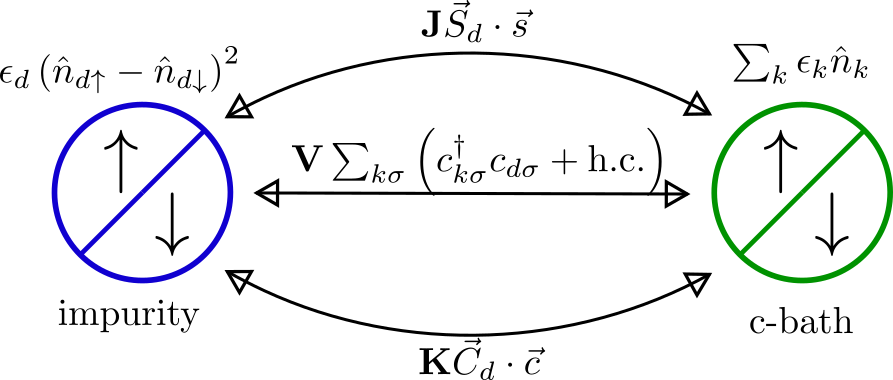
\includegraphics[width=0.6\textwidth]{../figures/gen_siam.png}
	\caption{Schematic diagram of the generalized SIAM model.}
\end{figure}
 There are eight different type of scattering terms:
\begin{equation}\begin{aligned}
	c^\dagger_{q\beta}T_1 &= V_1 c^\dagger_{q\beta}c_{d\beta}\hat n_{d\overline\beta}, &c^\dagger_{q\beta}T_2 &= V_0 c^\dagger_{q\beta}c_{d\beta}\left(1 - \hat n_{d\overline\beta}\right)\\
	c^\dagger_{q\beta}T_3 &= \sum_{k<\Lambda_N}J^z_0 \hat n_{d\beta}\left(1 - \hat n_{d\overline\beta}\right) c^\dagger_{q\beta}c_{k\beta}, &c^\dagger_{q\beta}T_4 &= -\sum_{k<\Lambda_N}J^z_1 \hat n_{d\overline\beta}\left(1 - \hat n_{d\beta}\right) c^\dagger_{q\beta}c_{k\beta}\\
	c^\dagger_{q\beta}T_5 &= \sum_{k<\Lambda_N}J^t c^\dagger_{d\overline\beta}c_{d\beta}c^\dagger_{q\beta}c_{k\overline\beta}, &c^\dagger_{q\beta}T_6 &= K_z^1 \sum_{k<\Lambda_N}\hat n_{d\beta}\hat n_{d\overline\beta}c^\dagger_{q\beta}c_{k\beta}\\
	c^\dagger_{q\beta}T_7 &= -K_z^0 \sum_{k<\Lambda_N}\left(1 - \hat n_{d\beta}\right)\left(1 - \hat n_{d\overline\beta}\right)c^\dagger_{q\beta}c_{k\beta}, &c^\dagger_{q\beta}T_8 &= K_t \sum_{k<\Lambda_N}c^\dagger_{q\beta}c^\dagger_{k\overline\beta}c_{d\overline\beta}c_{d\beta}\\
\end{aligned}\end{equation}

\section{Obtaining the RG equations}
\subsection{Particle Sector}
Renormalization is
\begin{equation}\begin{aligned}
	c^\dagger_{q\beta}T \eta = c^\dagger_{q\beta}\sum_{ij}T_i \eta_j
\end{aligned}\end{equation}
The terms that survive are
\begin{equation}\begin{aligned}
& c^\dagger_{q\beta}T \eta
= \sum_{i=1}^8\frac{1}{\omega_i - E_i}\hat n_{q\beta} T_i T_i^\dagger +\left(\frac{1}{\omega_2 - E_2} + \frac{1}{\omega_5 - E_5}\right)\hat n_{q\beta} \left(T_2 T_5^\dagger + T_5 T_2^\dagger \right) \\
& +\left(\frac{1}{\omega_2 - E_2} + \frac{1}{\omega_3 - E_3}\right)\hat n_{q\beta} \left(T_2 T_3^\dagger + T_3 T_2^\dagger \right) + \left(\frac{1}{\omega_3 - E_3} + \frac{1}{\omega_5 - E_5}\right)\hat n_{q\beta} \left(T_3 T_5^\dagger + T_5 T_3^\dagger \right) \\
& + \left(\frac{1}{\omega_1 - E_1} + \frac{1}{\omega_6 - E_6}\right)\hat n_{q\beta} \left(T_1 T_6^\dagger + T_6 T_1^\dagger \right) + \left(\frac{1}{\omega_1 - E_1} + \frac{1}{\omega_8 - E_8}\right)\hat n_{q\beta} \left(T_1 T_8^\dagger + T_8 T_1^\dagger \right) \\
& + \left(\frac{1}{\omega_6 - E_6} + \frac{1}{\omega_8 - E_8}\right)\hat n_{q\beta} \left(T_6 T_8^\dagger + T_8 T_6^\dagger \right)\\
&=\frac{|V_1|^2}{\xi_1}\left( 1 - \hat n_{d\beta} \right) \hat n_{d\overline\beta} + \frac{|V_0|^2}{\xi_2}\left( 1 - \hat n_{d\beta} \right) \left( 1 - \hat n_{d\overline\beta} \right) + \frac{1}{\xi_5}J_t^2 \left( 1 - \hat n_{d\beta} \right) \hat n_{d\overline\beta} c_{k^\prime\overline\beta}c^\dagger_{k\overline\beta} \\
&+ \frac{1}{4}\left[ {J_0^z}^2\frac{\hat n_{d\beta}\left( 1 - \hat n_{d\overline\beta} \right) }{\xi_3} + {J_1^z}^2\frac{\hat n_{d\overline\beta}\left( 1 - \hat n_{d\beta} \right)}{\xi_4} \right]c_{k^\prime\beta}c^\dagger_{k\beta} - \frac{1}{2} \left(\frac{1}{\xi_2} + \frac{1}{\xi_5}\right)J_t\left( 1 - \hat n_{d\beta}\right) \left(V_0 c^\dagger_{k\overline\beta}c_{d\overline\beta} + \text{h.c.}\right) \\
&- \frac{1}{2}\left(\frac{1}{\xi_2} + \frac{1}{\xi_3}\right)\frac{J^z_0}{2}\left(1 - \hat n_{d\overline\beta}\right)\left(V_0 c^\dagger_{k\beta}c_{d\beta} + \text{h.c.}\right) - \frac{1}{2}\left(\frac{1}{\xi_3} + \frac{1}{\xi_5}\right)\frac{J_t J^z_0}{2}\left(c^\dagger_{d\beta}c_{d\overline\beta}c^\dagger_{k\overline\beta}c_{k^\prime\beta} + \text{h.c.}\right) \\
&+ \left[\frac{{K_z^1}^2}{\xi_6}\hat n_{d\beta}\hat n_{d\overline\beta} + \frac{{K_z^0}^2}{\xi_7}\left(1 - \hat n_{d\beta}\right)\left(1 - \hat n_{d\overline\beta}\right)\right]c_{k^\prime\beta}c^\dagger_{k\beta} + \frac{K_t^2}{\xi_8}\left(1 - \hat n_{d\beta}\right)\left(1 - \hat n_{d\overline\beta}\right)c^\dagger_{k\overline\beta}c_{k^\prime\overline\beta}\\
&- \frac{1}{2}\left(\frac{1}{\xi_1} + \frac{1}{\xi_6} \right)V_1 K_z^1 \hat n_{d\overline\beta}\left(c^\dagger_{k\beta}c_{d\beta} + \text{h.c.}\right) + \frac{1}{2}\left(\frac{1}{\xi_1} + \frac{1}{\xi_8} \right)V_1 K_t \left(1 - \hat n_{d\beta}\right)\left(c^\dagger_{k\overline\beta}c_{d\overline\beta} + \text{h.c.}\right)\\
&- \frac{1}{2}\left(\frac{1}{\xi_6} + \frac{1}{\xi_8} \right)K_z^1 K_t \left(c^\dagger_{d\beta}c^\dagger_{d\overline\beta}c_{k^\prime\overline\beta}c_{k\beta} + \text{h.c.}\right)
\end{aligned}\end{equation}
where \(\xi_i = \omega_i - E_i\) and we substituted \(\hat n_{q\beta}=1\). The energies in the denominators are
\begin{equation}\begin{aligned}
E_1&= E_8 = \frac{\epsilon_q}{2} + 2\epsilon_d+ U - \frac{1}{2}K_z, &&E_2 = E_4 = E_5 = \frac{\epsilon_q}{2} + \epsilon_d - \frac{1}{2}J_z\\
E_3&=\frac{\epsilon_q}{2} + \epsilon_d + \frac{1}{2}J_z, &&E_6 =\frac{\epsilon_q}{2} + 2\epsilon_d+ U + \frac{1}{2}K_z\\
E_7&=\frac{\epsilon_q}{2} - \frac{1}{2}K_z, &&E_8=\frac{\epsilon_q}{2}+2\epsilon_d+ U  - \frac{1}{2}K_z
\end{aligned}\end{equation}
The quantum fluctuation scales are
\begin{equation}\begin{aligned}
\omega_1&=\omega + \epsilon_d+\frac{1}{2}K_z, &&\omega_3 =\omega+\epsilon_d + \frac{1}{2}K_z + J_z\\
\omega_2& = \omega_8 = \omega+\frac{1}{2}J_z, &&\omega_4 = \omega_5 = \omega + \epsilon_d + \frac{1}{2}K_z\\
\omega_6&=\omega+2\epsilon_d+U+\frac{1}{2}J_z + K_z, &&\omega_7 =\omega+\frac{1}{2}J_z\\
\end{aligned}\end{equation}
\subsection{Hole sector}
Renormalization is
\begin{equation}\begin{aligned}
&\eta c^\dagger_{q\beta}T = \left( 1 - \hat n_{q\beta} \right) \left[\sum_{i=1}^8\frac{1}{\omega^\prime_i - E^\prime_i} T_i T_i^\dagger +\left(\frac{1}{\omega^\prime_1 - E^\prime_1} + \frac{1}{\omega^\prime_4 - E^\prime_4}\right) \left(T_1 T_4^\dagger + T_4 T_1^\dagger \right)\right. \\
&\left. +\left(\frac{1}{\omega^\prime_1 - E^\prime_1} + \frac{1}{\omega^\prime_5 - E^\prime_5}\right) \left(T_1 T_5^\dagger + T_5 T_1^\dagger \right) + \left(\frac{1}{\omega^\prime_2 - E^\prime_2} + \frac{1}{\omega^\prime_7 - E^\prime_7}\right) \left(T_2 T_7^\dagger + T_7 T_2^\dagger \right) \right.\\
&\left. + \left(\frac{1}{\omega^\prime_2 - E^\prime_2} + \frac{2}{\omega^\prime_8 - E^\prime_8}\right) \left(T_2 T_8^\dagger + T_8 T_2^\dagger \right) + \left(\frac{1}{\omega^\prime_4 - E^\prime_4} + \frac{1}{\omega^\prime_5 - E^\prime_5}\right) \left(T_4 T_5^\dagger + T_5 T_4^\dagger \right) \right.\\
&\left. + \left(\frac{1}{\omega^\prime_7 - E^\prime_7} + \frac{1}{\omega^\prime_8 - E^\prime_8}\right)\hat n_{q\beta} \left(T_7 T_8^\dagger + T_8 T_7^\dagger \right)\right]\\
	&=\frac{|V_1|^2}{\xi^\prime_1}\hat n_{d\overline\beta}\hat n_{d\beta} + \frac{|V_0|^2}{\xi^\prime_2}\hat n_{d\beta}\left(1 - \hat n_{d\overline\beta}\right)+\frac{1}{4}\left[ {J_0^z}^2\frac{\hat n_{d\beta}\left( 1 - \hat n_{d\overline\beta} \right) }{\xi^\prime_3} + {J_1^z}^2\frac{\hat n_{d\overline\beta}\left( 1 - \hat n_{d\beta} \right)}{\xi^\prime_4} \right]c^\dagger_{k\beta}c_{k^\prime\beta} \\
	&+ \frac{1}{\xi^\prime_5}J_t^2 \left( 1 - \hat n_{d\overline\beta} \right) \hat n_{d\beta} c^\dagger_{k\overline\beta} c_{k^\prime\overline\beta} - \frac{1}{2} \left(\frac{1}{\xi^\prime_4} + \frac{1}{\xi^\prime_1}\right)\frac{J_1^z}{2}\hat n_{d\overline\beta} \left(V_1 c^\dagger_{k\beta}c_{d\beta} + \text{h.c.}\right) \\
	&- \frac{1}{2}\left(\frac{1}{\xi^\prime_1} + \frac{1}{\xi^\prime_5}\right)J_t \hat n_{d\beta}\left(V_1 c^\dagger_{k\overline\beta}c_{d\overline\beta} + \text{h.c.}\right) - \frac{1}{2}\left(\frac{1}{\xi^\prime_4} + \frac{1}{\xi^\prime_5}\right)\frac{J_t J^z_1}{2}\left(c^\dagger_{d\beta}c_{d\overline\beta}c^\dagger_{k\overline\beta}c_{k^\prime\beta} + \text{h.c.}\right)\\
&+\left[\frac{{K_z^1}^2}{\xi^\prime_6}\hat n_{d\beta}\hat n_{d\overline\beta} + \frac{{K_z^0}^2}{\xi^\prime_7}\left(1 - \hat n_{d\beta}\right)\left(1 - \hat n_{d\overline\beta}\right)\right]c^\dagger_{k\beta}c_{k^\prime\beta} + \frac{K_t^2}{\xi^\prime_8}\hat n_{d\beta}\hat n_{d\overline\beta}c_{k^\prime\overline\beta}c^\dagger_{k\overline\beta} \\
&- \frac{1}{2}\left(\frac{1}{\xi^\prime_2} + \frac{1}{\xi^\prime_7}\right)V_0 K_z^0\left(1 - \hat n_{d\overline\beta}\right)\left(c^\dagger_{k\beta}c_{d\beta} + \text{h.c.}\right) + \frac{1}{2}\left(\frac{1}{\xi^\prime_2} + \frac{1}{\xi^\prime_8}\right)V_0 K_t\hat n_{d\beta}\left(c^\dagger_{k\overline\beta}c_{d\overline\beta} + \text{h.c.}\right) \\
&- \frac{1}{2}\left(\frac{1}{\xi^\prime_7} + \frac{1}{\xi^\prime_8}\right)K_z^0 K_t\left(c^\dagger_{d\beta}c^\dagger_{d\overline\beta}c_{k\overline\beta}c_{k^\prime\beta} + \text{h.c.}\right) 
\end{aligned}\end{equation}
The denominator energies are
\begin{equation}\begin{aligned}
	E_1^\prime &= E_3^\prime = E_5^\prime = \frac{\epsilon_q}{2} + \epsilon_d - \frac{1}{2}J_z, &&E_4^\prime = \frac{\epsilon_q}{2} + \epsilon_d + \frac{1}{2}J_z\\
	E_2^\prime &= \frac{\epsilon_q}{2} - \frac{1}{2}K_z, &&E_7^\prime = \frac{\epsilon_q}{2} + \frac{1}{2}K_z\\
	E_6^\prime &= \frac{\epsilon_q}{2} + 2\epsilon_d + U - \frac{1}{2}K_z, &&E_8^\prime = \frac{\epsilon_q}{2} + \epsilon_d - \frac{1}{2}K_z\\
\end{aligned}\end{equation}
The quantum fluctuation scales are
\begin{equation}\begin{aligned}
	\omega_1^\prime&=\omega+2\epsilon_d+U+\frac{1}{2}J_z\\
	\omega_2^\prime&=\omega+\epsilon_d+\frac{1}{2}K_z \\
	\omega_3^\prime&=\omega_5^\prime=\omega+\epsilon_d + \frac{1}{2}K_z\\
	\omega_4^\prime&=\omega+\epsilon_d+\frac{1}{2}K_z + J_z \\
	\omega_6^\prime&=\omega+2\epsilon_d+U+\frac{1}{2}J_z\\
	\omega_7^\prime&=\omega+\frac{1}{2}J_z + K_z\\
	\omega_8^\prime &=\omega+\epsilon_d+\frac{1}{2}J_z \\
\end{aligned}\end{equation}
\subsection{Scaling equations}
The denominators \(\xi_i,\xi_i^\prime\) are
\begin{equation}\begin{aligned}
	\xi_1 &= \omega - \frac{\epsilon_q}{2} - \epsilon_d - U + K_z\\
	\xi_2 &= \omega - \frac{\epsilon_q}{2} - \epsilon_d + J_z\\
	\xi_3 &= \xi_4 = \xi_5 = \xi_6 = \xi_7 = \omega - \frac{\epsilon_q}{2} + \frac{1}{2}J_z + \frac{1}{2}K_z\\
	\xi_8 &= \omega - \frac{\epsilon_q}{2} - 2\epsilon_d - U + \frac{1}{2}J_z + \frac{1}{2}K_z\\
	\xi_1^\prime &= \omega - \frac{\epsilon_q}{2} + \epsilon_d + U + J_z\\
	\xi_2^\prime &= \omega - \frac{\epsilon_q}{2} + \epsilon_d + K_z\\
	\xi_3^\prime &= \xi_4^\prime = \xi_5^\prime = \xi_6^\prime = \xi_7^\prime = \omega - \frac{\epsilon_q}{2} + \frac{1}{2}J_z + \frac{1}{2}K_z\\
	\xi_8^\prime &= \omega - \frac{\epsilon_q}{2} + 2\epsilon_d + U + \frac{1}{2}J_z + \frac{1}{2}K_z\\
\end{aligned}\end{equation}
The RG equations are
\begin{equation}\begin{aligned}
	\Delta \epsilon_d &= \frac{|V_1|^2}{\xi_1} + \frac{|V_0|^2}{\xi_2^\prime} - 2 \frac{|V_0|^2}{\xi_2} - \sum_k\left( \frac{K_z^2}{2\xi_6} + \frac{K_t^2}{\xi_8} - \frac{J_z^2}{2\xi_3} - \frac{J_t^2}{\xi_3}\right) \\
	\Delta U &= \frac{2|V_1|^2}{\xi^\prime_1} + \frac{2|V_0|^2}{\xi_2} - \frac{2|V_1|^2}{\xi_1} - \frac{2|V_0|^2}{\xi_2^\prime} + 2\sum_k\left(\frac{K_z^2}{2\xi_6} + \frac{K_t^2}{\xi_8} - \frac{J_z^2}{2\xi_3} - \frac{J_t^2}{\xi_3}\right) \\
	\Delta V_1 &= - \frac{1}{4}\left[ V_1 \frac{K_z}{2}\left( \frac{1}{\xi_1} + \frac{1}{\xi_6} \right) - V_0 K_t \left( \frac{1}{\xi_2^\prime} + \frac{1}{\xi_8^\prime} \right)\right] - V_1 \left( \frac{J_z}{2} + J_t \right) \left( \frac{1}{\xi_1^\prime} + \frac{1}{\xi_3} \right) \\
	\Delta V_0 &= - \frac{1}{4}\left[ V_0 \frac{K_z}{2}\left( \frac{1}{\xi_2^\prime} + \frac{1}{\xi_7^\prime} \right) - V_1 K_t \left( \frac{1}{\xi_1} + \frac{1}{\xi_8} \right)\right] - V_0 \left( \frac{J_z}{2} + J_t \right) \left( \frac{1}{\xi_2} + \frac{1}{\xi_3} \right) \\
	\Delta J_z &= - 2 \frac{J_t^2}{\xi_3}\\
	\Delta J_t &= - 2 \frac{J_z J_t}{\xi_3}\\
	\Delta K_z &= - 2 \frac{K_t^2}{\xi_8}\\
	\Delta K_t &= - \frac{K_z K_t}{2}\left( \frac{1}{\xi_6} + \frac{1}{\xi_8} + \frac{1}{\xi_7^\prime} + \frac{1}{\xi_8^\prime}\right) \\
\end{aligned}\end{equation}
Note that these are the renormalizations are for each momentum state \(q\) on the isoenergetic shell - the total renormalization is obtained by summing over the \(q\).
\section{Numerical and analytical analysis of the symmetric model}
\subsection{Nature of RG flows for the symmetric model at \(V = 0\)}
With the conditions \(\epsilon_d = -\epsilon_d - U, J_z = J_t = \frac{1}{2}J, V_0 = V_1, K_z = K_t = \frac{1}{2}K\),
\begin{equation}\begin{aligned}
	\Delta U &= \sum_k \frac{3}{4}\frac{K^2 - J^2}{\omega - \frac{\epsilon_q}{2} + \frac{1}{4}J + \frac{1}{4}K} \\
	\Delta J &= - \frac{J^2}{\omega - \frac{\epsilon_q}{2} + \frac{1}{4}J + \frac{1}{4}K}\\
	\Delta K &= - \frac{K^2}{\omega - \frac{\epsilon_q}{2} + \frac{1}{4}J + \frac{1}{4}K}\\
\end{aligned}\end{equation}
For \(\omega - \frac{\epsilon_q}{2} + \frac{1}{4}J + \frac{1}{4}K > 0\), the flow is towards a weak coupling theory, but these are not URG fixed points. Such flows are shown in fig.~\ref{Jdecay}. For the rest of the values of \(\omega\), we get RG flows towards a strong-coupling fixed point, with large value of \(J\) and \(K\), fig.~\ref{J_sc}. For sufficiently small values of \(\frac{J}{K}\), the flow is towards zero \(U\). All such flows characterise a resonant-level strong coupling fixed point, where the four atomic impurity levels are degenerate and located exactly at the Fermi surface. For larger values of \(\frac{J}{K}\), there exist flows towards a large positive \(U\). Such fixed points energetically favour an impurity occupation of \(1\). Both these classes of flows of \(U\) are depicted in fig.~\ref{U_flow}.
\begin{figure}[htpb]
	\centering
	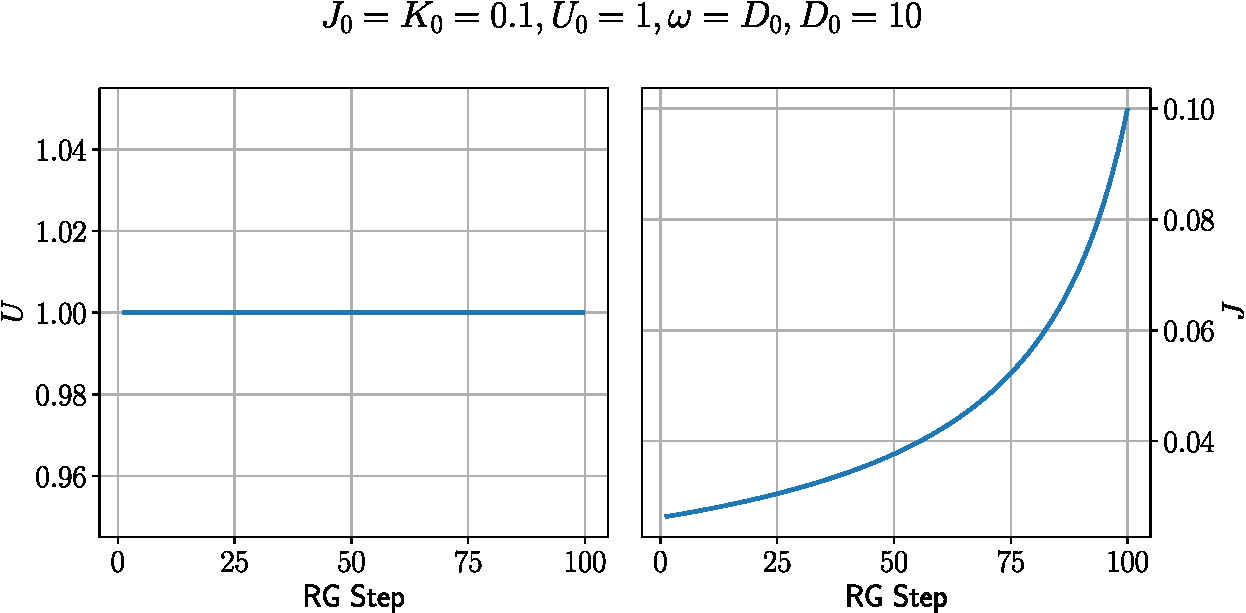
\includegraphics[width=\textwidth]{../figures/large_w.pdf}
	\caption{Large \(\omega\). Right Decay of \(J\) towards zero under RG. Left Flow of \(U\) under the same RG. Titles of plots show bare values.}
	\label{Jdecay}
\end{figure}
\begin{figure}[htpb!]
	\centering
	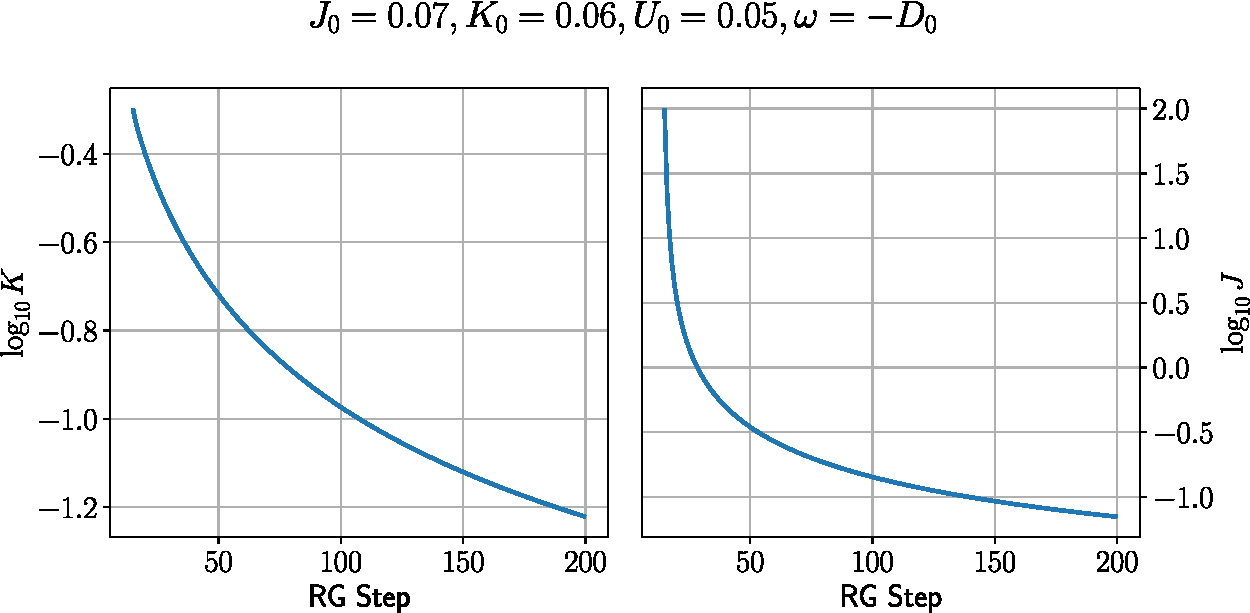
\includegraphics[width=\textwidth]{../figures/low_w_JK.pdf}
	\caption{Small \(\omega\). Flow of \(J\) and \(K\) to large values, signaling a strong-coupling fixed point.}
	\label{J_sc}
\end{figure}
\begin{figure}[htpb]
	\centering
	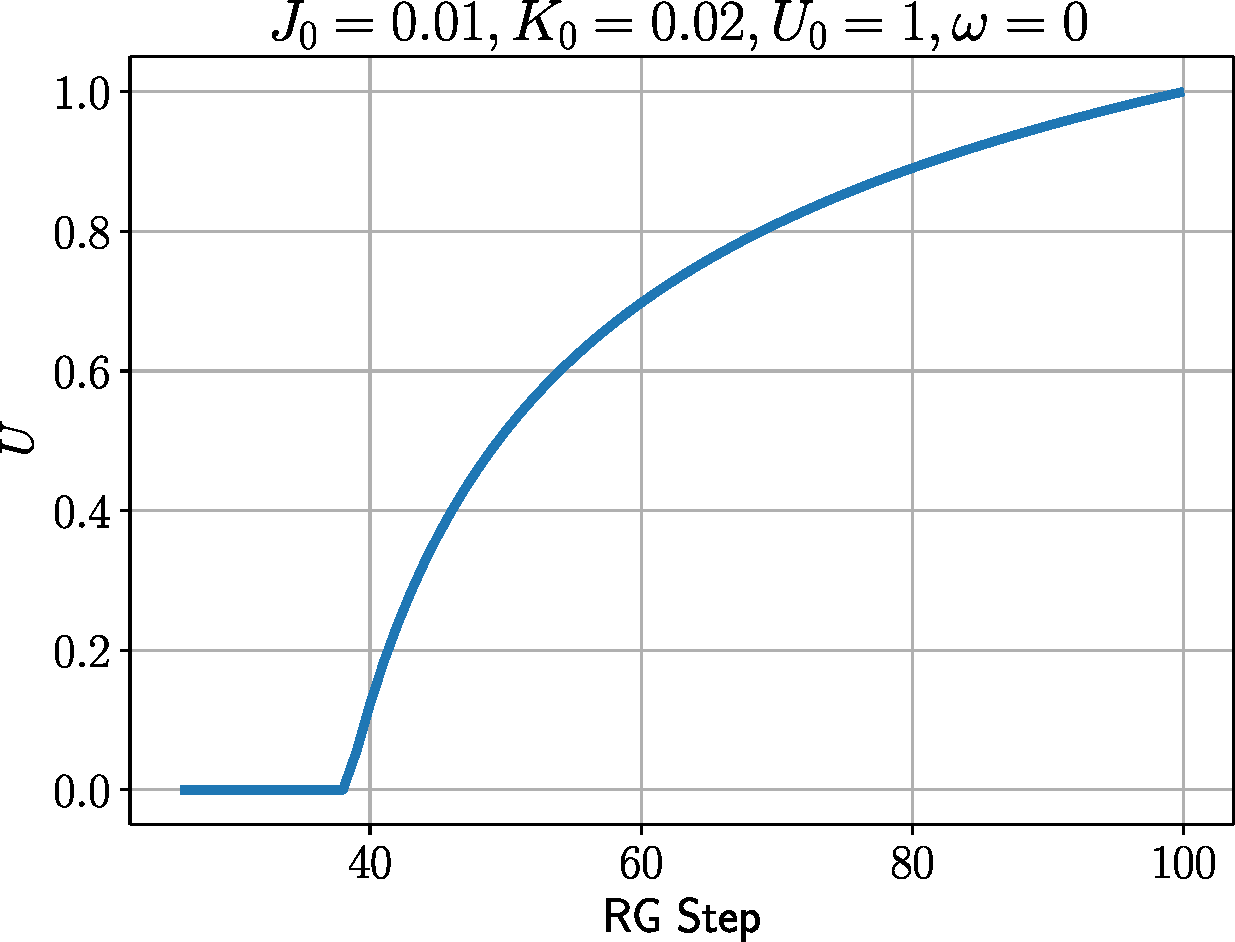
\includegraphics[width=0.49\textwidth]{../figures/U_irr.pdf}
	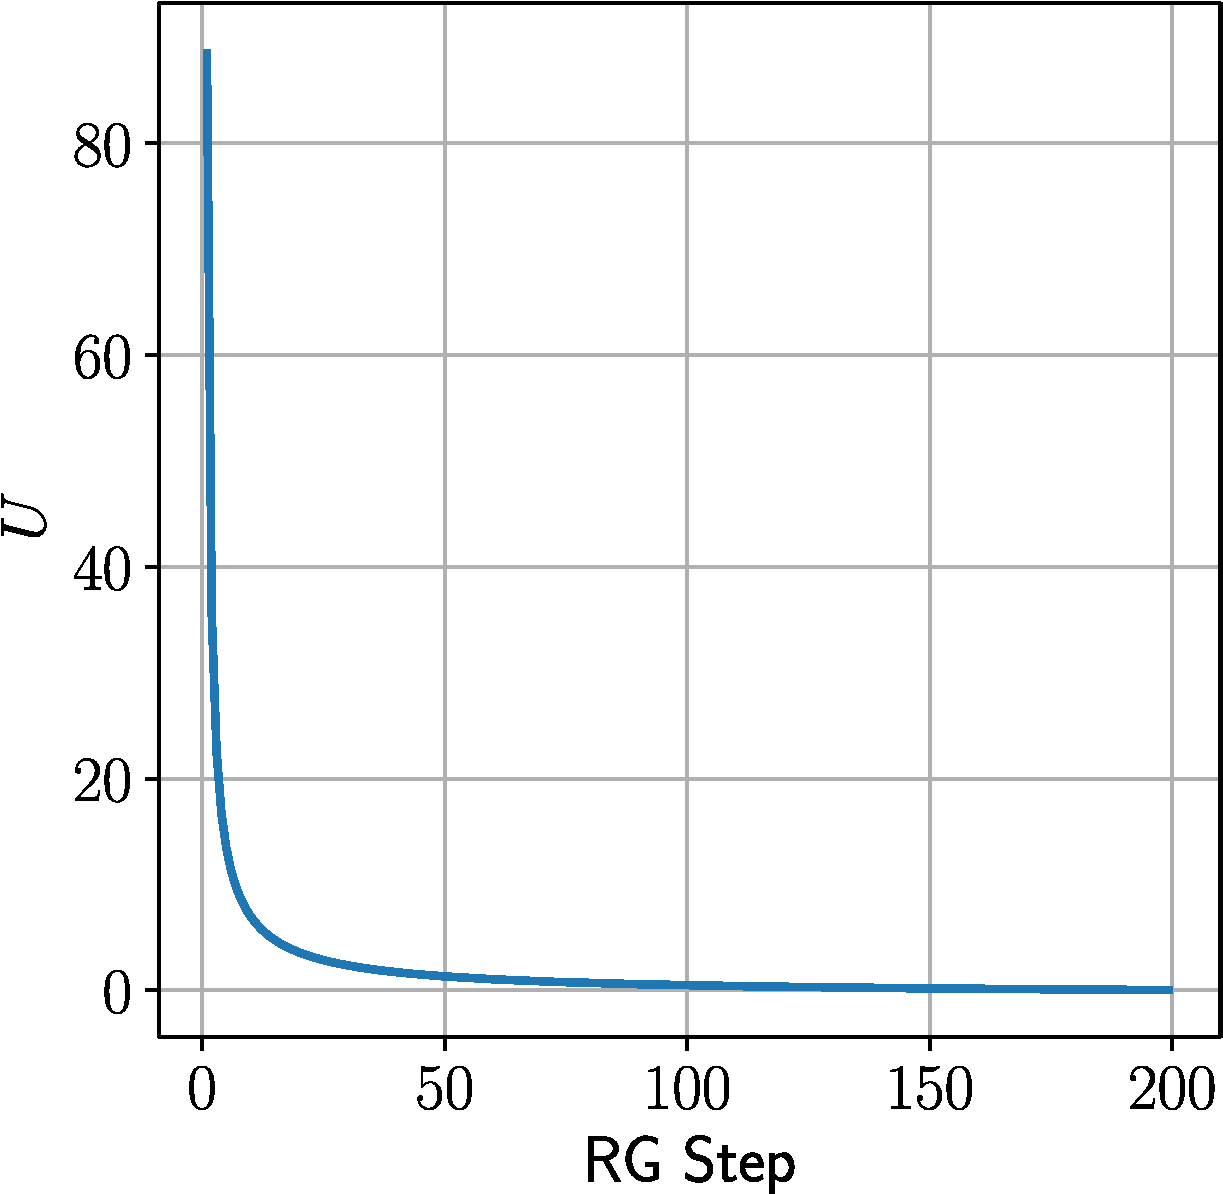
\includegraphics[width=0.49\textwidth]{../figures/U_rel.pdf}
	\caption{Left: Flow of \(U\) to zero, implying a four-fold degenerate impurity. Right: Flow of \(U\) to large value, making the impurity singly-occupied, leading to the formation of a local moment.}
	\label{U_flow}
\end{figure}
From the RG equations for \(J\) and \(K\), we can write down an RG-invariant.
\begin{equation}\begin{aligned}
	\label{rginv}
	\frac{\Delta J}{\Delta K} = \frac{J^2}{K^2} \implies \frac{1}{J} - \frac{1}{K} = \mathcal{C} = \frac{1}{J_0} - \frac{1}{K_0}
\end{aligned}\end{equation}
where \(\mathcal{C}\) is a constant. For the case of \(J_0 = K_0\) (\(J_0\) is the bare value of \(J\)), we must have \(J=K\). The RG flows in the \(K \text{ vs } J\) plane are shown in fig.~\ref{JvsK}.
\begin{figure}[htpb]
	\centering
	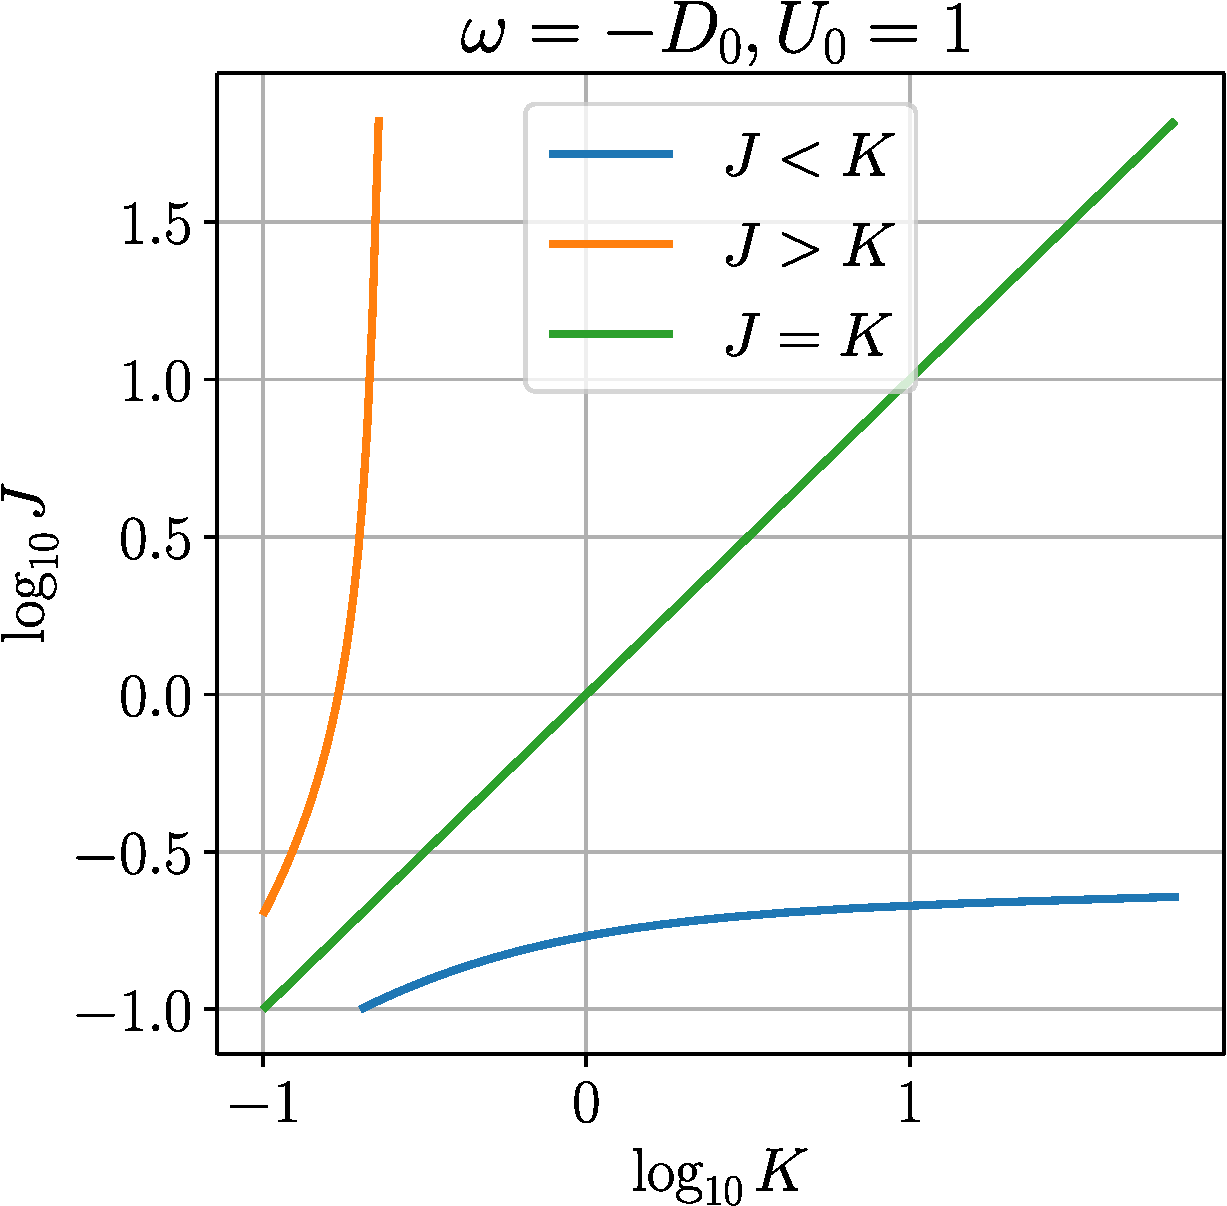
\includegraphics[width=0.6\textwidth]{../figures/JvsK.pdf}
	\caption{RG flows in \(K\) vs \(J\) plane. Legend indicates relations of bare values.}
	\label{JvsK}
\end{figure}
\subsection{Eigenstates of symmetrical model at \(V=0\)}
For the case of \(V=0\), the RG equations simplify considerably.
\begin{equation}\begin{aligned}
	\Delta U &= 2\sum_k \frac{3}{8}\frac{K^2 - J^2}{\omega - \frac{\epsilon_q}{2} + \frac{1}{4}J + \frac{1}{4}K} \\
	\Delta J &= - \frac{J^2}{\omega - \frac{\epsilon_q}{2} + \frac{1}{4}J + \frac{1}{4}K}\\
	\Delta K &= - \frac{K^2}{\omega - \frac{\epsilon_q}{2} + \frac{1}{4}J + \frac{1}{4}K}\\
\end{aligned}\end{equation}
The strong-coupling fixed points is reached for \(\omega - \frac{\epsilon_q}{2} + \frac{1}{4}J + \frac{1}{4}K < 0\). Since the denominator is thus negative, we will have
\begin{equation}\begin{aligned}
	\Delta U \begin{cases}
		> 0, & J> K \\
		< 0, & J< K
	\end{cases}
\end{aligned}\end{equation}
This implies that for \(J>K\), the flow is towards an impurity which is singly-occupied, while \(J < K\) will mean the impurity will be four-fold degenerate with all four levels at the Fermi surface. 
\\\\The effective Hamiltonian is
\begin{equation}\begin{aligned}
	\mathcal{H}^* = \sum_{k\sigma} \epsilon_k \hat n_{k\sigma} - 2 U^* \left(S_d^z\right)^2 + \sum_{kk^\prime < \Lambda^*}\left[J^* \vec{S_d}\cdot\vec{s_{kk^\prime}} + K^* \vec{C_d}\cdot\vec{C_{kk^\prime}}\right] + \sum_{q > \Lambda^*}\left[J_q S_d^z s^z_{q} + K_q C_d^z C^z_{q}\right]
\end{aligned}\end{equation}
where \(S_d^z = \frac{1}{2}\left( \hat n_{d\uparrow} - \hat n_{d \downarrow} \right) \). Since the interaction terms do not couple the \(\hat n_{d}=1\) and \(\hat n_{d}=0,2\) subspaces, we can diagonalize the Hamiltonian separately in these subspaces. 
\\\\In the singly-occupied subspace, the Hamiltonian is
\begin{equation}\begin{aligned}
	\mathcal{H}^*_{1} = \sum_k \epsilon_k \hat n_{k\sigma} - \frac{1}{2} U^* + \sum_{kk^\prime < \Lambda^*}J^* \vec{S_d}\cdot\vec{s_{kk^\prime}}+ \sum_{q > \Lambda^*}J^{**} S_d^z s^z_{q}
\end{aligned}\end{equation}
The ground state in this subspace is
\begin{equation}\begin{aligned}
	\ket{\Psi}^*_{1}= \frac{1}{\mathcal{N}}\sum_{kk^\prime < \Lambda^*\atop{q>\Lambda^*}}\left[\ket{S_d^z= \frac{1}{2}}\ket{s^z_{kk^\prime}= - \frac{1}{2}}\ket{s^z_{q}= - \frac{1}{2}} - \ket{S_d^z=- \frac{1}{2}}\ket{s^z_{kk^\prime}=  \frac{1}{2}}\ket{s^z_{q}=  \frac{1}{2}}\right]
\end{aligned}\end{equation}
with an eigenvalue (besides the energy of the bath)
\begin{equation}\begin{aligned}
	E_{1} = - \frac{U^*}{2} - \frac{3}{4}J^* - \frac{1}{4}J^{**}
\end{aligned}\end{equation}
In the complementary subspace, the Hamiltonian is
\begin{equation}\begin{aligned}
	\mathcal{H}^*_{0,2} = \sum_k \epsilon_k \hat n_{k\sigma} + \sum_{kk^\prime < \Lambda^*}K^* \vec{C_d}\cdot\vec{C_{kk^\prime}}+ \sum_{q > \Lambda^*}K^{**} C_d^z C^z_{q}
\end{aligned}\end{equation}
The ground state in this subspace is
\begin{equation}\begin{aligned}
	\ket{\Psi}^*_{0,2}= \frac{1}{\mathcal{N^\prime}}\sum_{kk^\prime < \Lambda^*\atop{q>\Lambda^*}}\left[\ket{C_d^z= \frac{1}{2}}\ket{C^z_{kk^\prime}= - \frac{1}{2}}\ket{C^z_{q}= - \frac{1}{2}} - \ket{C_d^z=- \frac{1}{2}}\ket{C^z_{kk^\prime}=  \frac{1}{2}}\ket{C^z_{q}=  \frac{1}{2}}\right]
\end{aligned}\end{equation}
with an eigenvalue (besides the energy of the bath)
\begin{equation}\begin{aligned}
	E_{0,2} = - \frac{3}{4}K^* - \frac{1}{4}K^{**}
\end{aligned}\end{equation}
Depending on the bare values of \(J,K\) and \(U\), we can have the following fixed point situations:
\begin{table}[htpb]
\centering
\begin{tabular}{|c|c|c|c|c|c|c|}
\hline
\(U \) & \(J,K \) & \(U^*\) &\(J^*,K^*\) & class & ground state & ground state energy\\
\hline
\(>0\)& \(J > K\)& \(\gg 0\)&\(J^*>K^*\) & screened spin & spin singlet & \(- \frac{U^*}{2} - \frac{3}{4}J^* - \frac{1}{4}J^{**}\)\\
\(>0\)& \(J < K\)& \(0\) &\(J^*<K^*\) & screened charge & charge singlet & \(- \frac{3}{4}K^* - \frac{1}{4}K^{**}\)\\
\(<0\)& \(J > K\)& \(0\) &\(J^*>K^*\) & screened spin & spin singlet& \(- \frac{3}{4}J^* - \frac{1}{4}J^{**}\)\\
\(<0\)& \(J < K\)& \(\ll 0\)&\(J^*<K^*\) & screened charge & charge singlet & \(- \frac{3}{4}K^* - \frac{1}{4}K^{**}\)\\
\hline
\end{tabular}
\caption{Classification of fixed points for various bare values, at \(V=0\)}
\label{classes}
\end{table}
\begin{figure}[htpb!]
	\centering
	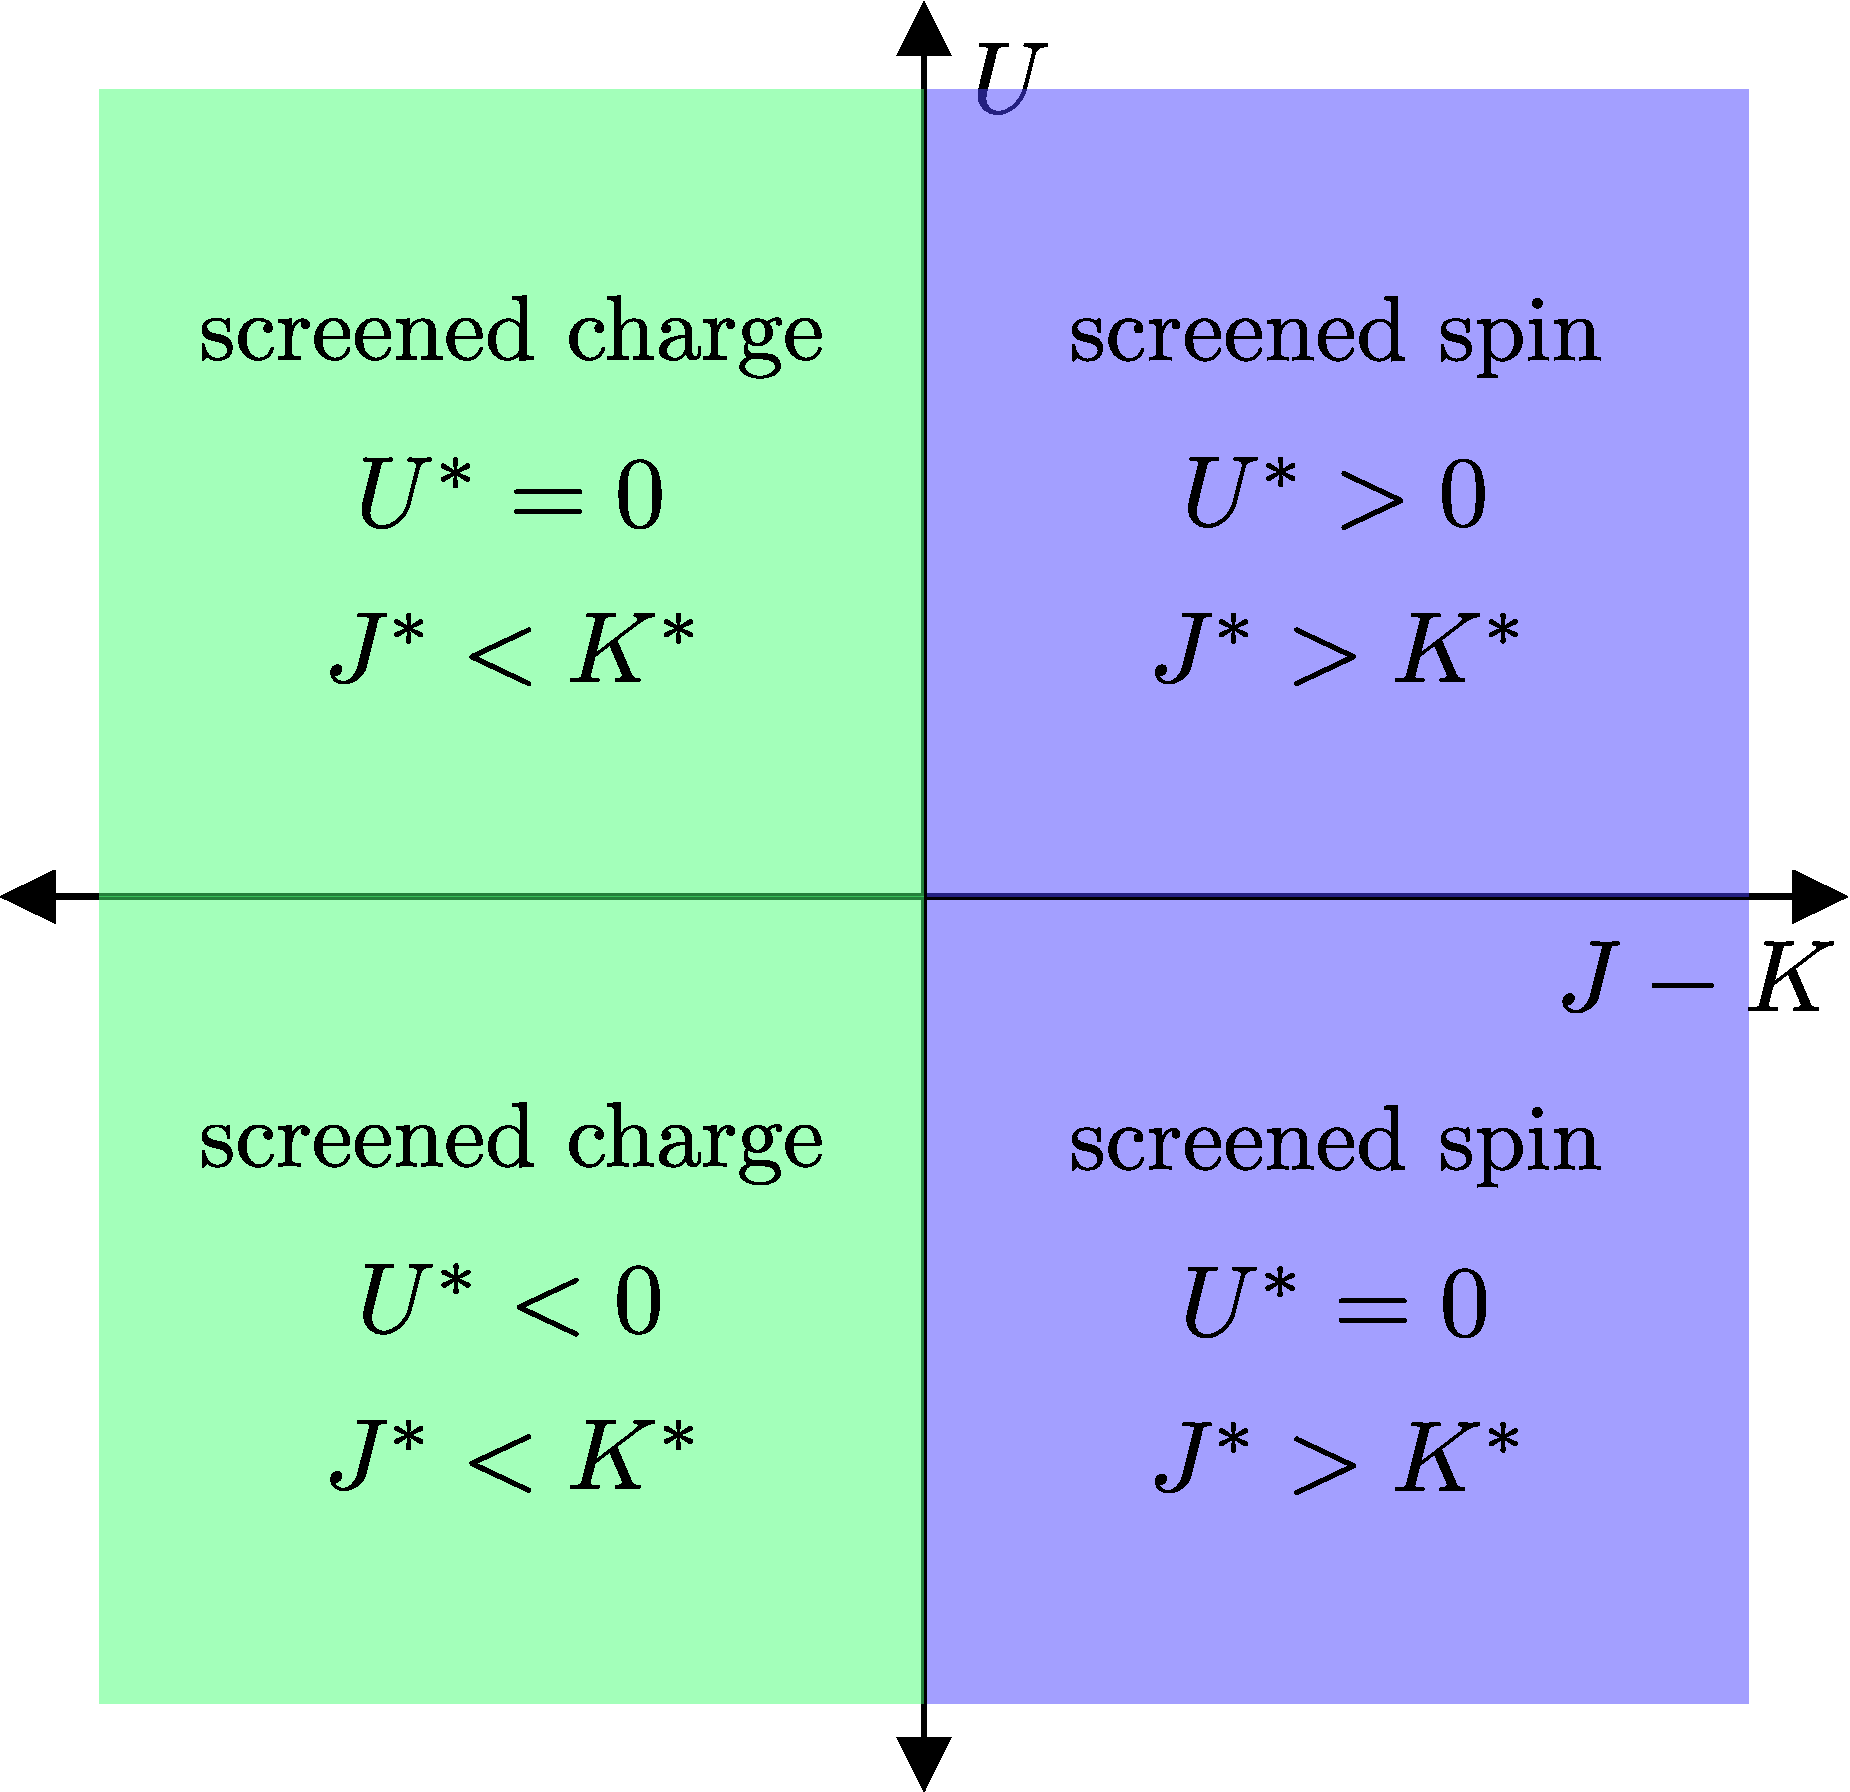
\includegraphics[scale=0.2]{../figures/phases.pdf}
	\caption{Fixed point phases in the plane of bare couplings, at \(V=0\).}
	\label{siamphases}
\end{figure}
\subsection{Effect of non-zero \(V\) on the RG flows}
The introduction of \(V\) into the RG equations make them analytically intractable, and we have to solve them numerically. The general observation is that we now get both zero and non-zero values of \(U^*\) in all the phases. The low quantum fluctuation scale behaviour in the first quadrant is shown in fig.~\ref{Veffect}. It is very similar to that obtained from NRG, as was shown in fig.~\ref{nrg_fp}.
\begin{figure}[htpb]
	\centering
	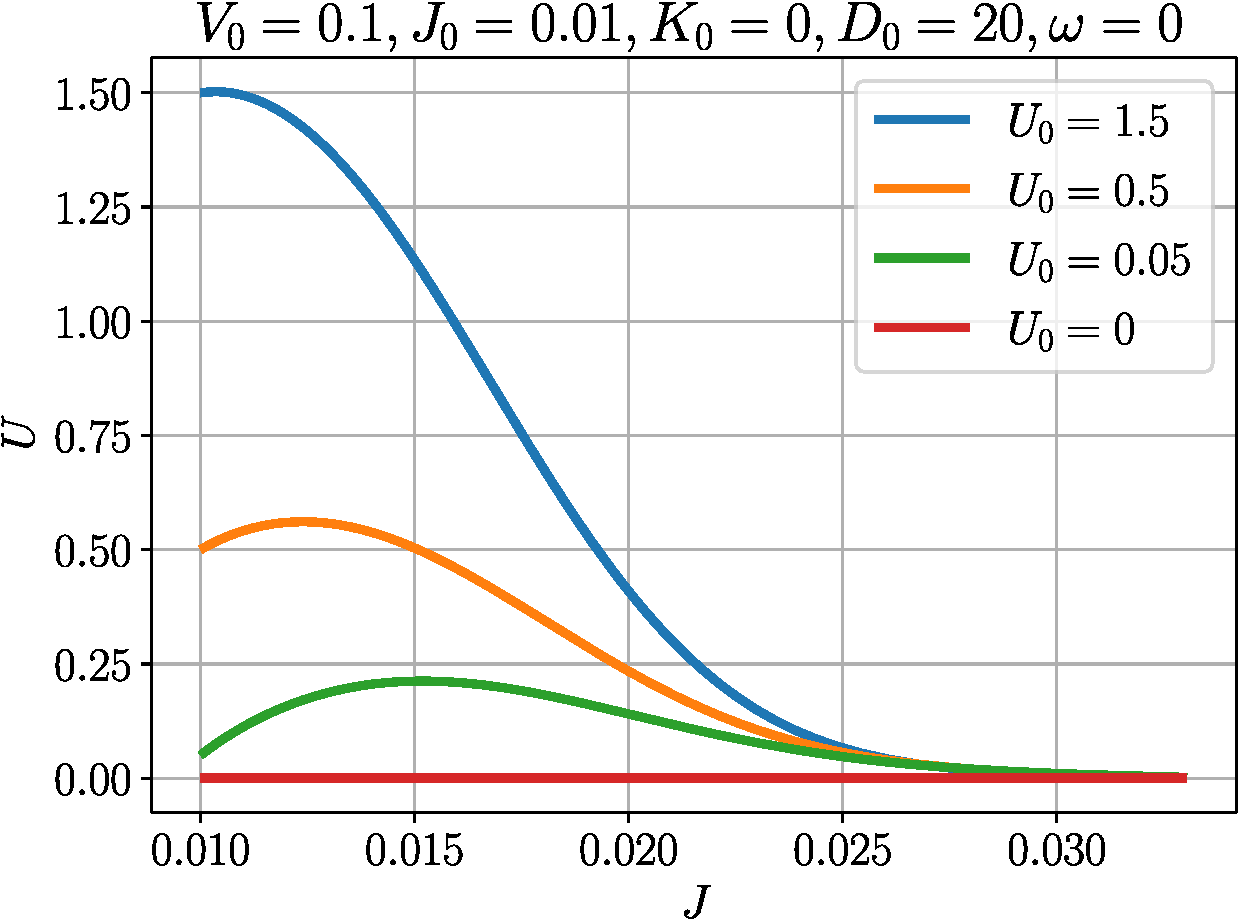
\includegraphics[width=0.8\textwidth]{../figures/UvsJ_new.pdf}
	\caption{\(U-J\) multiple RG flows in first quadrant.}
	\label{Veffect}
\end{figure}

\begin{figure}[htpb!]
	\centering
	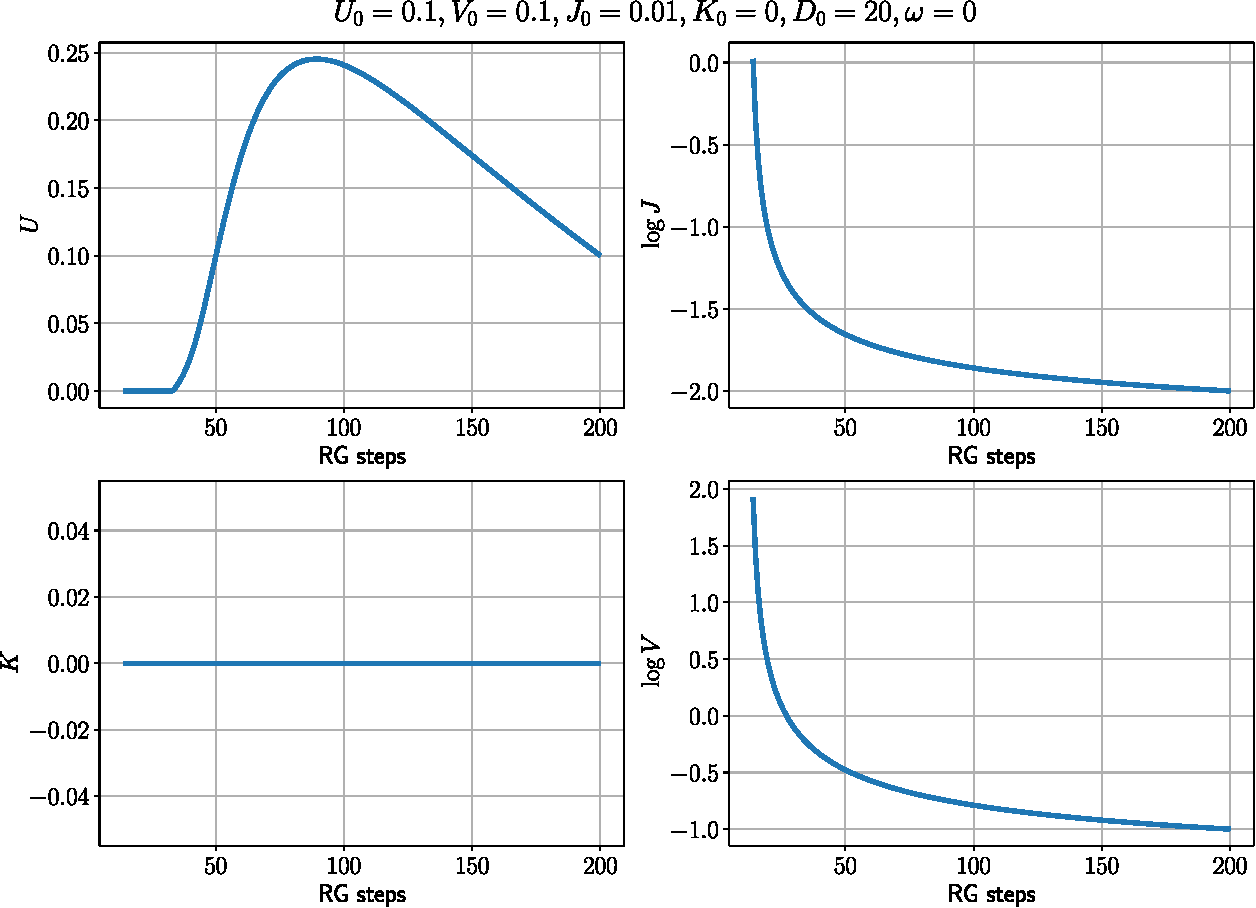
\includegraphics[width=\textwidth]{../figures/with_V_new.pdf}
	\caption{Flows of the couplings for bare values in the first quadrant: \(J-K,U>0\).}
	% \label{Veffect}
\end{figure}
\paragraph*{First quadrant}
The first quadrant shows the flow from a free orbital fixed point near \(V=U=J=0\) to an intermediate local moment phase with large \(U\) with a final crossover to a stable fixed point at \(J^* \gg J_0, U^*=0\). The initial free orbital fixed point involves four degenerate impurity states at the impurity, and hence no local moment. The intermediate phase involves a local moment because of the large \(U\). The final stable phase involves an impurity which is strongly-coupled to the impurity because of the large \(V\) and \(J\). This crossover is depicted in fig.~\ref{crossover}.


\begin{figure}[htpb]
	\centering
	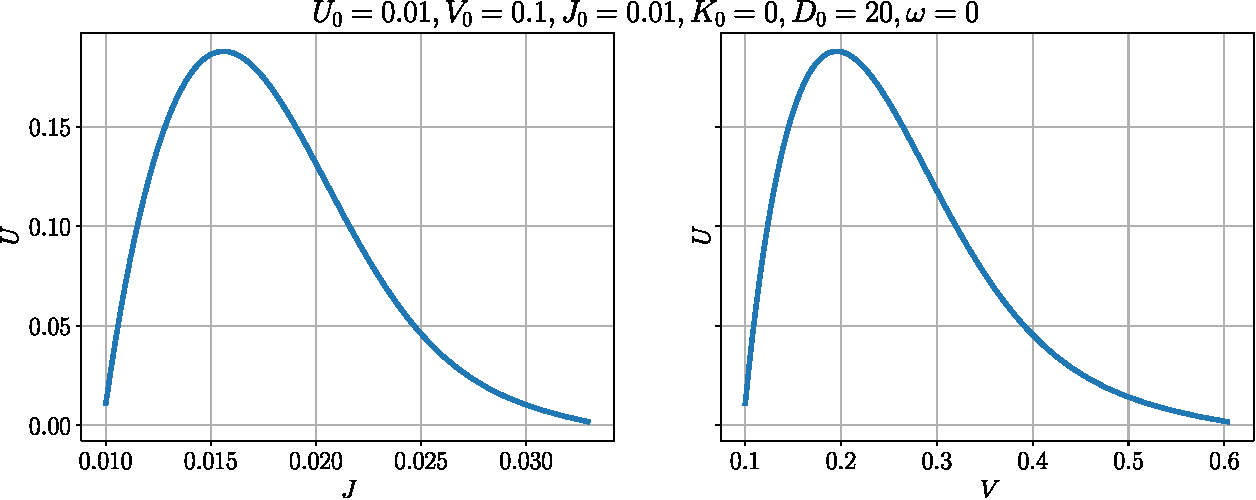
\includegraphics[width=\textwidth]{../figures/crossovers_new.pdf}
	\caption{\(U-J\) and \(U-V\) RG flows.}
	\label{crossover}
\end{figure}

We have also checked that the fixed point values of \(J\) and \(V\) go on increasing as we increase the system size.

\begin{figure}[htpb]
	\centering
	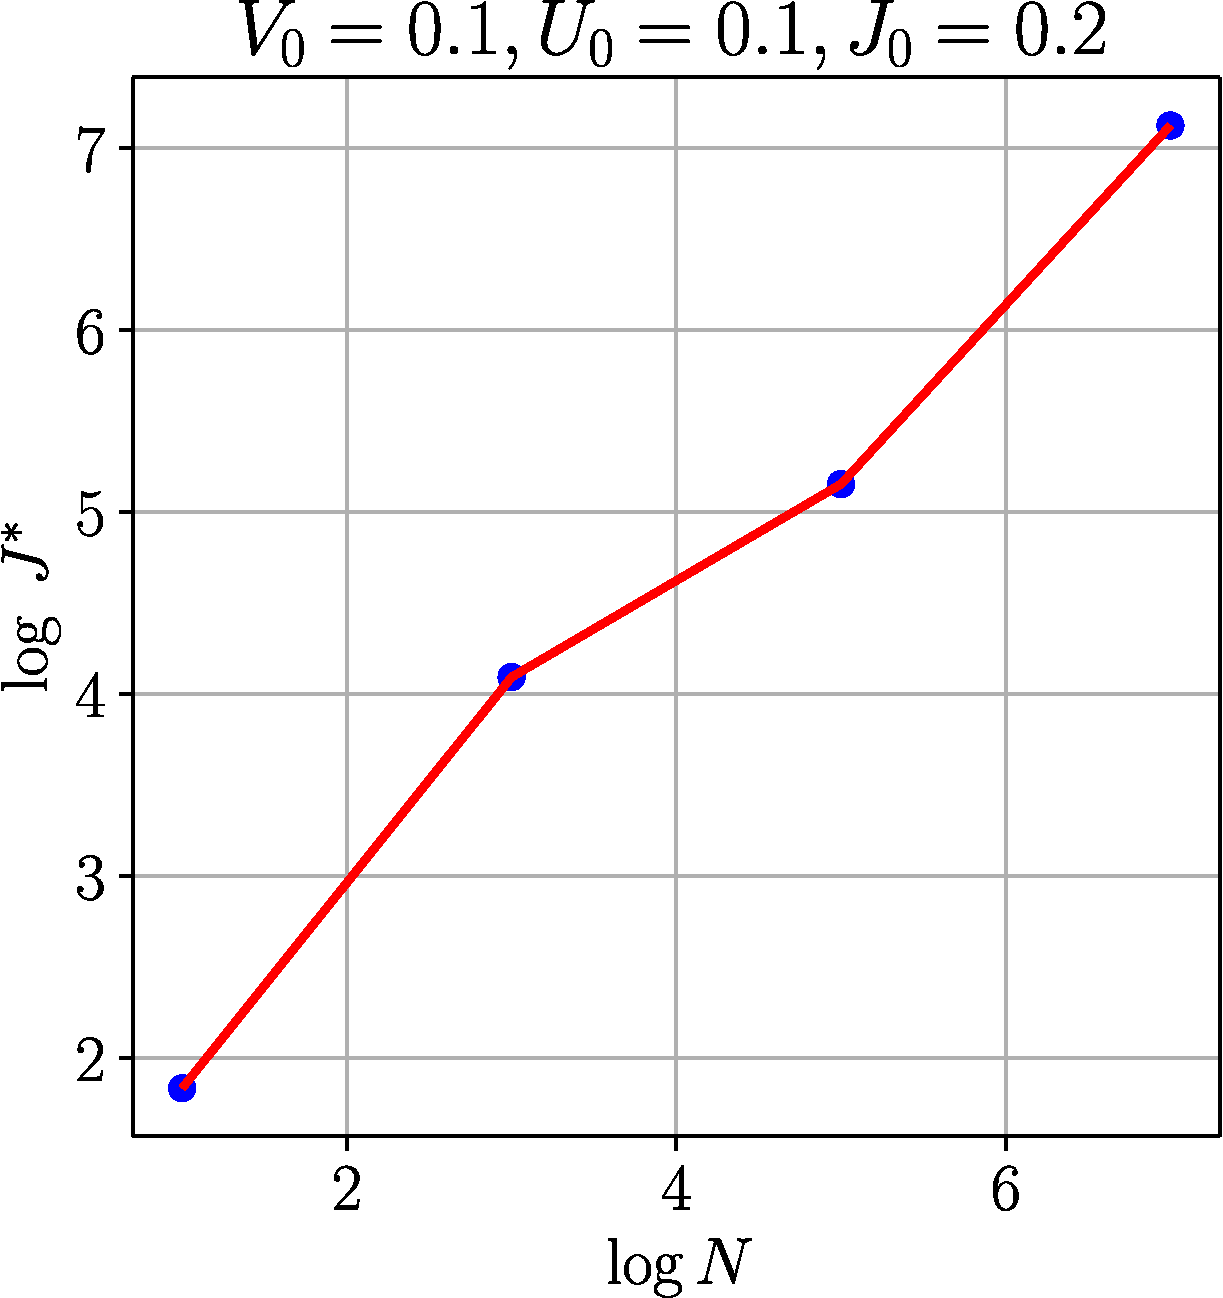
\includegraphics[width=0.49\textwidth]{../figures/J_vs_D_q1.pdf}
	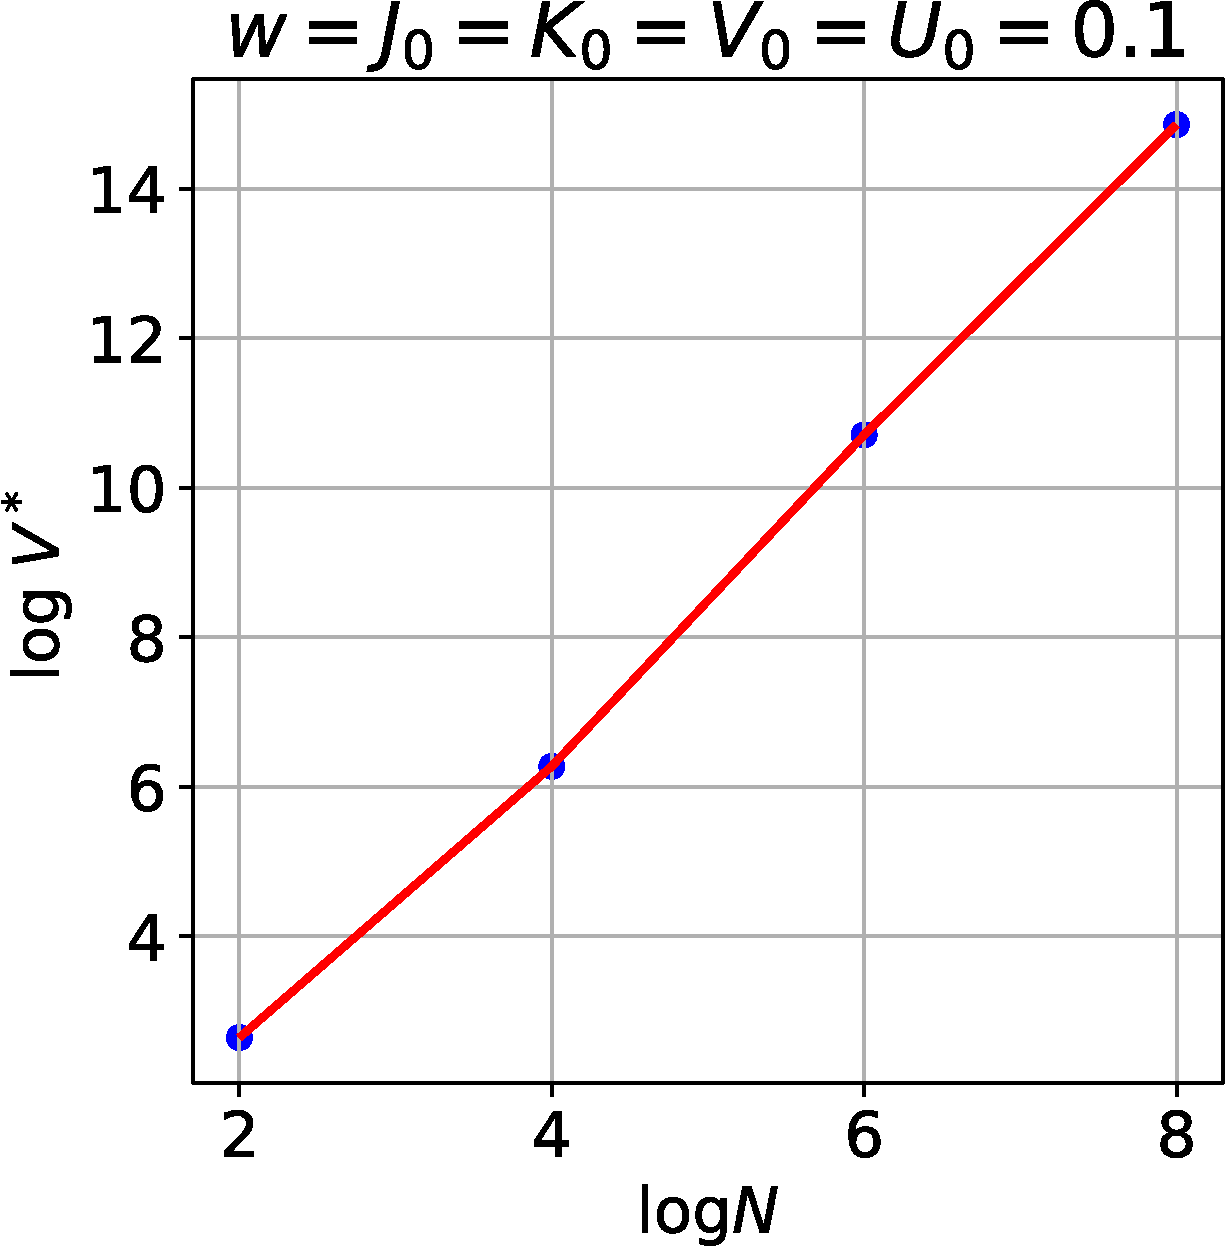
\includegraphics[width=0.49\textwidth]{../figures/V_vs_D_q1.pdf}
	\caption{Increase in the fixed point values of \(J\) and \(V\) with system size.}
	\label{JV-system-size}
\end{figure}
\paragraph*{Third quadrant}
In the third quadrant (\(U_0 < 0, K_0 > J_0\)), we see the flow to large negative value of \(U\), leading to a large contribution of the holon-doublon sectors of the impurity subspace, and a large value of \(K^*\) which means that the impurity charge sector couples very strongly with the bath charge sector.
\begin{figure}[htpb!]
\centering
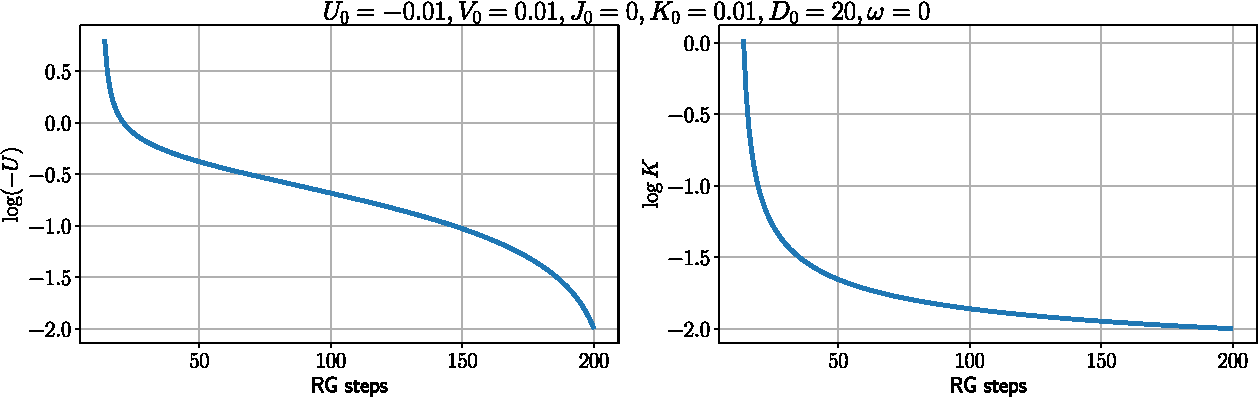
\includegraphics[width=\textwidth]{../figures/with_V_q3_new.pdf}
\caption{Flow of \(U\) to large negative value and \(K\) to large positive value in the third quadrant.}
\label{frac_q3}
\end{figure}
This is essentially the charge analogue of the Kondo effect; the relevant transformation is
\begin{equation}\begin{aligned}
	\ket{\uparrow} \to \ket{2}, \ket{\downarrow} \to \ket{0}, J \to K, U \to -U
\end{aligned}\end{equation}
The ground state in this sector will be a charge singlet, as shown in the next section. This was also reported by Taraphder and Coleman in \cite{taraphder}.
\subsection{Phase diagram for \(V > 0\)}
We can now summarize the various fixed point phases. The physically relevant ones are the first and third quadrants. The first quadrant features a large spin-exchange coupling \(J\) and a positive \(U\) in the bare model, and the stable flows are towards a large \(J^*\) and a very small (\(\approx 0\)) \(U^*\). The fixed point state will be mostly a spin singlet, in which the impurity polarization gets quenched by the spin-flip scattering of the conduction electrons. The third quadrant is the regime of the charge-Kondo effect, and involves a negative \(U\) at the bare level which physically motivates a large charge-Kondo coupling \(K\). The fixed point again involves flow to a large \(K^*\), but the \(U\) flows to large negative here, implying a state where the charge sectors dominate heavily and the ground state is primarily a charge-singlet in which the destruction or annihilation of the Cooper-pair like states becomes prohibited.
\\\\These results are summarized in the table below.
\begin{table}[htpb]
\centering
\begin{tabular}{|c|c|c|c|c|c|c|}
\hline
\(U \) & \(J,K \) & \(U^*\) &\(J^*,K^*\) & class & ground state \\
\hline
\(>0\)& \(J > K\)& \(\gtrsim 0\)&\(J^*>K^*\) & screened spin & spin singlet + charge triplet\\
\(>0\)& \(J < K\)& \(\gtrsim 0\) &\(J^*<K^*\) & screened charge & charge singlet\\
\(<0\)& \(J > K\)& \(\gtrsim 0\) &\(J^*>K^*\) & screened spin & spin singlet + charge triplet\\
\(<0\)& \(J < K\)& \(\ll 0\)&\(J^*<K^*\) & screened charge & charge singlet\\
\hline
\end{tabular}
\caption{Classification of fixed points for various bare values, at \(V > 0\)}
\end{table}

\begin{figure}[htpb!]
	\centering
	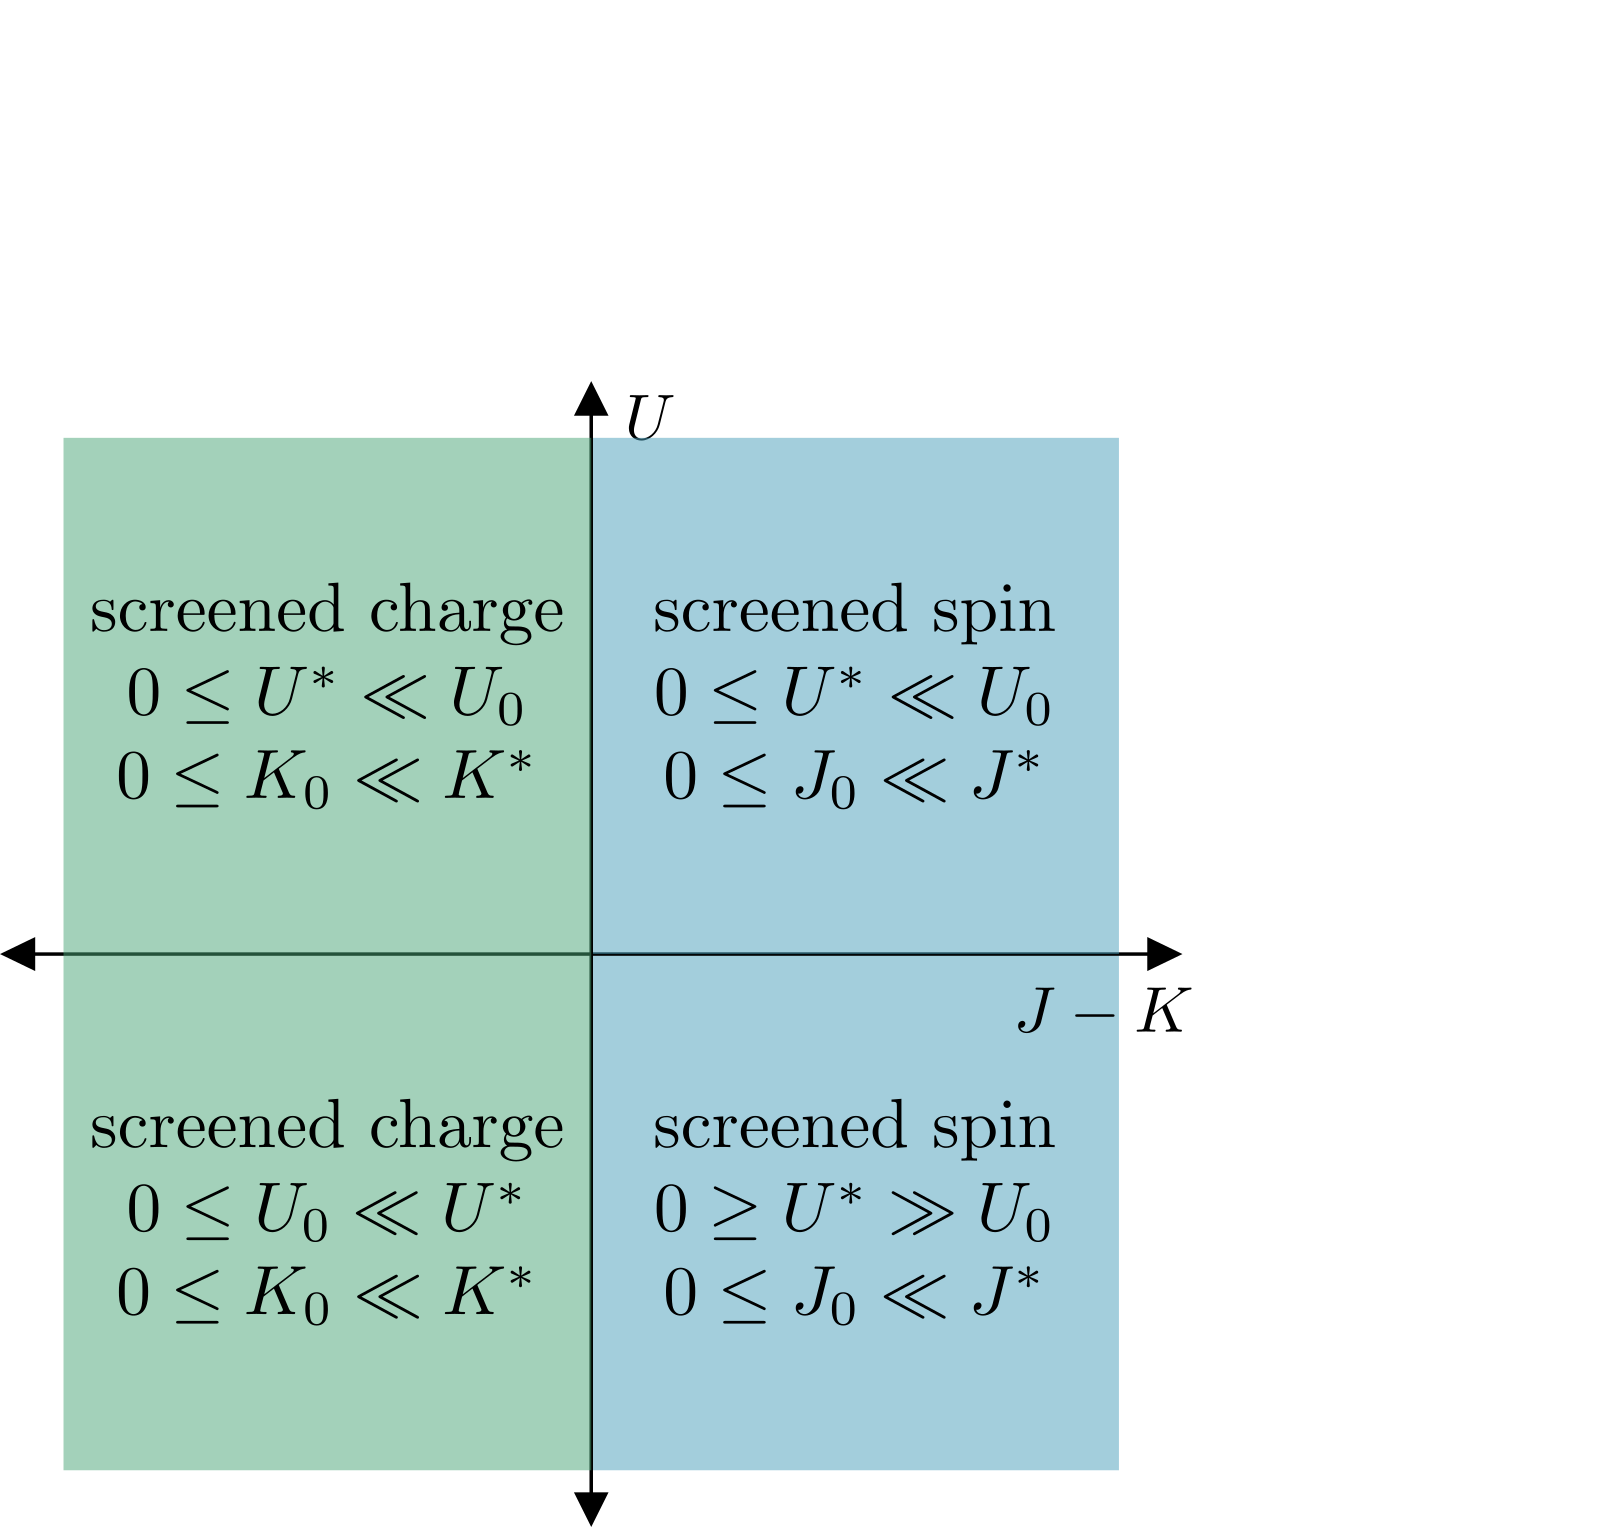
\includegraphics[width=0.4\textwidth]{../figures/phases_V.png}
	\caption{Low \(\omega\) fixed point phases for the SIAM with \(V>0\).}
\end{figure}

\section{Effective Hamiltonian and ground state for the \(V\neq 0\) symmetric problem}
The fixed point Hamiltonian can be written, in general, as
\begin{equation}\begin{aligned}
	\mathcal{H}^* = \sum_{\sigma, k}\epsilon_k \tau_{k\sigma} - \frac{U^*}{2}\hat n_d + U^* \hat n_{d\uparrow}\hat n_{d\downarrow} + \sum_{\sigma, k < \Lambda^*}\left( V^* c^\dagger_{k\sigma}c_{d\sigma} + \text{h.c.} \right) + J^* \vec{S_d}\cdot\vec{s} + K^* \vec{C_d}\cdot\vec{C} \\
	+ \sum_{q > \Lambda^*}\left(J^z_q S^z_ds^z_q + K^z_q C^z_dC^z_q\right) 
\end{aligned}\end{equation}
The first term is the kinetic energy of all the electrons. The next two terms are the impurity-diagonal pieces, featuring the renormalised interaction \(U^*\). The next three terms are the residual interactions between the impurity and the metal, with the renormalised couplings \(V^*, J^*\) and \(K^*\). The summations in these terms extend from the fixed point momentum cutoff \(\Lambda^*\) to 0. This is the region of momentum space  which the URG was unable to decouple. The operators \(\vec s\) and \(\vec C\) represent the macroscopic magnetic and charge spins formed by the remaining electrons that are lying inside the window \(\left[ 0, \Lambda^* \right] \):
\begin{equation}\begin{aligned}
	\vec s = \sum_{kk^\prime<\Lambda^*\atop{\alpha\beta}} c^\dagger_{k\alpha}\vec \sigma_{\alpha\beta}c_{k^\prime\beta}
\end{aligned}\end{equation}
The final two terms represent the diagonal pieces of the RG steps that have been completed. These survive because the URG removes only the number-off-diagonal terms; terms like \(S^d_z s_z\) and \(C^d_z C_z\) conserve the number of particles and hence survive. These will also be renormalised, and hence the subscript \(q\) on \(J^z_q\) signifies that it is has been renormalised up to a certain momentum.
\\\\Our goal here is to write down the ground state wavefunction for the low-energy Hamiltonian
\begin{equation}\begin{aligned}
	\label{fixed_point_ham}
	\mathcal{H}_{IR} = \sum_{\sigma, k<\Lambda^*}\epsilon_k \tau_{k\sigma} - \frac{U^*}{2}\hat n_d + U^* \hat n_{d\uparrow}\hat n_{d\downarrow} + \sum_{\sigma, k < \Lambda^*}\left( V^* c^\dagger_{k\sigma}c_{d\sigma} + \text{h.c.} \right) + J^* \vec{S_d}\cdot\vec{s} + K^* \vec{C_d}\cdot\vec{C}
\end{aligned}\end{equation}
To make progress with the ground state, we will simplify the effective Hamiltonian by mapping it onto a two-site problem. One site is of course the impurity site. The other site will be formed by the centre of mass degree of freedom of the conduction electrons, which we define as
\begin{equation}\begin{aligned}
	c_{2\sigma} \equiv \frac{1}{\sqrt{N^*}}\sum_{k} c_{k\sigma} = c_\sigma\left( \vec r = 0 \right) 
\end{aligned}\end{equation}
where \(N^*\) is the number of electrons inside the window \(\left[-\Lambda^*, \Lambda^*\right]\). This operator essentially creates a conduction electron at the origin. It is easy to prove that this operator is Fermionic:
\begin{equation}\begin{aligned}
	\label{site2antic}
	\left\{c_{2\sigma}, c^\dagger_{2\sigma} \right\}  &= \frac{1}{N^*}\sum_{kk^\prime} \left\{ c_{k\sigma}, c^\dagger_{k^\prime\sigma} \right\} = \frac{1}{N^*}\sum_{kk^\prime} \delta_{kk^\prime} = 1\\
	\left\{c_{2\sigma}, c_{2\sigma} \right\}  &= \frac{1}{N^*}\sum_{kk^\prime} \left\{ c_{k\sigma}, c_{k^\prime\sigma} \right\} = 0
\end{aligned}\end{equation}
The number operator corresponding to this degree of freedom is
\begin{equation}\begin{aligned}
	\hat n_{2\sigma} = c^\dagger_{2\sigma}c_{2\sigma} = \frac{1}{N^*}\sum_{kk^\prime}c^\dagger_{k\sigma}c_{k^\prime\sigma}
\end{aligned}\end{equation}
Because of the anticommutation algebra in eq.~\ref{site2antic}, this operator behaves essentially like a Fermion: \(\hat n_{2\sigma}^2 = \hat n_{2\sigma}\). For our two-site problem, we will imagine this to be the annihilation operator for the site 2, for the spin sigma. The corresponding operator for the first site is of course just the impurity electron annihilation operator:
\begin{equation}\begin{aligned}
	c_{1\sigma} \equiv c_{d\sigma}
\end{aligned}\end{equation}
The various terms of the Hamiltonian can now be written in terms of these operators. We write the Fourier decomposition of the dispersion of the conduction bath.
\begin{equation}\begin{aligned}
	\epsilon_{\vec{k}} = \frac{1}{N^*}\sum_{\vec r}e^{i \vec{k}\cdot\vec{r}}\epsilon(\vec r)
\end{aligned}\end{equation}
The inverse transformation is
\begin{equation}\begin{aligned}
	\epsilon(\vec r) = \sum_{|\vec k| < \Lambda^*}e^{-i \vec{k}\cdot\vec{r}}\epsilon_{\vec{k}}
\end{aligned}\end{equation}
We now make a simplifying assumption: Guided by the observation that the important degree of freedom at the fixed point is the COM operator \(c_{2\sigma}\), we keep only the \(\vec r=0\) mode of the decomposition:
\begin{equation}\begin{aligned}
	\epsilon_{\vec k} \approx \frac{1}{N^*}\epsilon(\vec r=0) = \frac{1}{N^*}\sum_{k<\Lambda^*}\epsilon_k = \frac{1}{N^*}\sum_{\epsilon_k \in [\epsilon_F - D^*, \epsilon_F + D^*]}\epsilon_k = \epsilon_F
\end{aligned}\end{equation}
\(\epsilon_F\) is the Fermi energy, which we henceforth set to 0. The energy term for the second site is thus simply zero. The impurity diagonal part of \(\mathcal{H}_{IR}\) will survive only when \(\hat n_d = \hat n_1 = 1\). So we write it as
\begin{equation}\begin{aligned}
	- \frac{U^*}{2}\hat n_d + U^* \hat n_{d\uparrow}\hat n_{d\downarrow} = - \frac{U^*}{2}\left(\hat n_{d\uparrow} + \hat n_{d \downarrow} - 2\hat n_{d\uparrow}\hat n_{d\downarrow}\right) = - \frac{U^*}{2} \left(\hat n_{1 \uparrow} - \hat n_{1 \downarrow}\right)^2 \equiv \epsilon_d \left(\hat n_{1 \uparrow} - \hat n_{1 \downarrow}\right)^2
\end{aligned}\end{equation}
where \(\epsilon_d = - \frac{U^*}{2}\). The off-diagonal terms can also be similarly transformed into a two-site problem. The bath spin can be written as
\begin{equation}\begin{aligned}
	\vec S_d &\equiv \vec S_1\\
	J^*\vec s &= J^* \frac{1}{2}\sum_{kk^\prime\atop{\alpha\beta}}c^\dagger_{k\alpha}\vec \sigma_{\alpha\beta}c_{k^\prime\beta} \\
	       &= J^*\frac{1}{2}\sum_{\alpha\beta}c^\dagger_{2\alpha}\vec \sigma_{\alpha\beta}c_{2\beta} \\
	       &= J^* N^* \frac{1}{2}\left[\hat z\left(c^\dagger_{2 \uparrow}c_{2 \uparrow} - c^\dagger_{2 \downarrow} c_{2 \downarrow} \right) + \hat x \left(c^\dagger_{2 \uparrow}c_{2 \downarrow} + c^\dagger_{2 \downarrow} c_{2 \uparrow} \right) -i \hat y \left( c^\dagger_{2 \uparrow}c_{2 \downarrow} - c^\dagger_{2 \downarrow} c_{2 \uparrow} \right)\right]\\
	       &\equiv J^*N^* \vec S_2\\
	       &\equiv j \vec S_2\\
\end{aligned}\end{equation}
where \(j \equiv J^* N^*\) and
\begin{equation}\begin{aligned}
	\vec S_2 = \frac{1}{2N^*}\sum_{kk^\prime\atop{\alpha\beta}}c^\dagger_{k\alpha}\vec \sigma_{\alpha\beta}c_{k^\prime\beta}
\end{aligned}\end{equation}
. The charge isospins can also be rewritten similarly. From eq.~\ref{diagonalCz},
\begin{equation}\begin{aligned}
	K^* C^z &=K^* \frac{1}{2}\sum_{kk^\prime}\left( c^\dagger_{k \uparrow}c_{k^\prime \uparrow} - c_{k^\prime \downarrow}c^\dagger_{k \downarrow} \right) = \frac{1}{2}N^* K^*\left( c^\dagger_{2 \uparrow}c_{2 \uparrow} - c_{2 \downarrow}c^\dagger_{2\downarrow} \right) = kC_2^z\\
	K^* C^x &=K^* \frac{1}{2}\sum_{kk^\prime}\left( c^\dagger_{k \uparrow}c^\dagger_{k^\prime \downarrow} + c_{k \downarrow}c^\dagger_{k^\prime \uparrow} \right) = \frac{1}{2}N^* K^*\left( c^\dagger_{2 \uparrow}c_{2 \downarrow} - c_{2 \downarrow}c^\dagger_{2\uparrow} \right) = kC_2^x\\
\end{aligned}\end{equation}
and similarly for \(C^y\). We defined \(k \equiv K^* N^*\). The diagonal component \(C^z\) can also be written as
\begin{equation}\begin{aligned}
	 C^z = \frac{1}{2}N^* \sum_\sigma\left(c^\dagger_{2\sigma}c_{2\sigma} - \frac{1}{2}\right) = \frac{1}{2}N^*\tau_2
\end{aligned}\end{equation}
where \(\tau_2 = \sum_\sigma \tau_{2\sigma} = \sum_\sigma \left( \hat n_{2\sigma} - \frac{1}{2} \right) \). The hybridisation term can be written as
\begin{equation}\begin{aligned}
	V\sum_k c^\dagger_{k\sigma} = V\sqrt{N^*} c^\dagger_{2\sigma} = vc^\dagger_{2\sigma}
\end{aligned}\end{equation}
where \(v \equiv V\sqrt{N^*}\). The charge isospins can be written down similarly. Combining these, the interaction part can be written as
\begin{equation}\begin{aligned}
v\sum_{\sigma}\left( c^\dagger_{1\sigma}c_{2\sigma} + \text{h.c.} \right) + j\vec{S_1}\cdot\vec{S_2} + k\vec{C_1}\cdot\vec{C_2}
\end{aligned}\end{equation}
with \(k = K^* N^*\). The total Hamiltonian for the two-site problem is
\begin{equation}\begin{aligned}
	\mathcal{H}_{IR} = \epsilon_d m_1^2 + v\sum_{\sigma}\left(c^\dagger_{1\sigma}c_{2\sigma} + \text{h.c.} \right) + j\vec{S_1}\cdot\vec{S_2} + k \vec{C_1}\cdot\vec{C_2}
\end{aligned}\end{equation}
where we have dropped the \(*\) on the couplings for brevity and \(\hat n_{1 \uparrow} - \hat n_{1 \downarrow}=m_1\) is the magnetization on the first site. We will use the following notation to represent kets of this two-site system: \(\ket{n_{1 \uparrow}n_{1 \downarrow}n_{2 \uparrow}n_{2 \downarrow}}\). For example, a state \(\ket{1001}\) represents a ket with an up electron on site 1 and a down electron on site 2. This Hamiltonian conserves the total number operator \(\hat n \equiv \hat n_1 + \hat n_2\), so we can analyse the various subspaces corresponding to particular values of \(\hat n\) separately.
\begin{figure}[htpb]
	\centering
	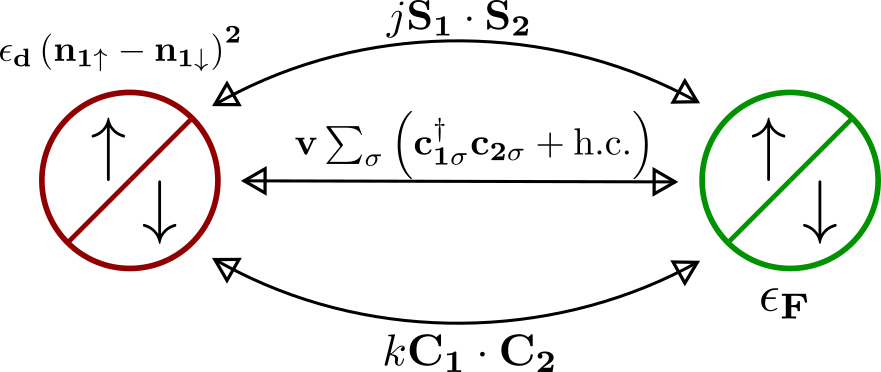
\includegraphics[width=0.6\textwidth]{../figures/two_site_problem.png}
	\caption{Two-site effective problem of fixed point Hamiltonian}
	\label{twosite}

\end{figure}
\\\\We will adopt the following notation to represent the states in this Hilbert space. A general state will be represented in the Fock space basis as \(\ket{n_{1 \uparrow}n_{1 \downarrow}n_{2 \uparrow}n_{2 \downarrow}}\). For example,
\begin{equation}\begin{aligned}
	\ket{1101} = c^\dagger_{1 \uparrow}c^\dagger_{1 \downarrow}c^\dagger_{2 \downarrow}\ket{-}
\end{aligned}\end{equation}
\(\ket{-}\) is the vacuum state.
\\\\First lets get the trivial cases of \(\hat n = 0, 4\) out of the way. The only possible states are \(\ket{0000}\) and \(\ket{1111}\) respectively. Both these states are eigenstates because the first one has no electron to scatter, and the second one has no vacant state to scatter into. These states have energy eigenvalues \( \frac{1}{4}k\)
\\\\The subspaces \(\hat n = 1,3\) are each four-dimensional. More precisely speaking, the \(\hat n=1\) subspace can have the following basis
\begin{equation}\begin{aligned}
	\ket{\uparrow,0}, \ket{0,\uparrow}, \ket{\downarrow,0}, \ket{0,\downarrow}
\end{aligned}\end{equation}
However, since the Hamiltonian conserves the total spin (both magnetic and charge), we can divide this Hilbert subspace into two smaller subspaces which do not talk to each other - one having the states \(\ket{\uparrow,0}, \ket{0,\uparrow}\) and hence a total spin magnetization of \(+\frac{1}{2}\), and the other having the remaining states and a total spin magnetization of \(-\frac{1}{2}\). The action of the Hamiltonian on this subspace is
\begin{equation}\begin{aligned}
	\mathcal{H}_{IR} \ket{1000} &= \left[\epsilon_d m_1^2 + vc^\dagger_{2 \uparrow}c_{1 \uparrow}\right] c^\dagger_{1 \uparrow}\ket{-} = \epsilon_d\ket{1000} + v\ket{0010}\\
	\mathcal{H}_{IR} \ket{0010} &= \left[\epsilon_d m_1^2 + vc^\dagger_{1 \uparrow}c_{2 \uparrow}\right] c^\dagger_{2 \uparrow}\ket{-} = v\ket{1000}\\
\end{aligned}\end{equation}
The Hamiltonian in first subspace can be represented by the matrix
\begin{equation}\begin{aligned}
	\label{n1mat}
	\bordermatrix{~&\ket{\uparrow,0} & \ket{0,\uparrow} \\
		~&\epsilon_d & v \\
		~& v & 0 \\
	}
\end{aligned}\end{equation}
The eigenstates (un-normalised) are
\begin{equation}\begin{aligned}
\label{low}
	-4v\ket{\uparrow,0} +2 \left[ \epsilon_d \mp \Delta\left(\epsilon_d , v\right)\right] \ket{0, \uparrow}, && E^1_\pm = \frac{1}{2} \epsilon_d \pm \frac{1}{2}\Delta\left(\epsilon_d , v\right)
\end{aligned}\end{equation}
where \(\Delta\left(\epsilon_d , v\right)  = \sqrt{\epsilon_d^2 + 4 v^2}\). The other two eigenstates (corresponding to magnetization \(- \frac{1}{2}\) need not be calculated separately; since the Hamiltonian is invariant under the transformation \( \uparrow \leftrightarrow \downarrow\), we can do a similar transformation on the eigenkets to get the eigenkets for the other subspace.
\begin{equation}\begin{aligned}
	-4v\ket{\downarrow,0} + 2 \left[ \epsilon_d \mp \Delta\left(\epsilon_d , v \right)\right] \ket{0, \downarrow}
\end{aligned}\end{equation}
with exactly the same eigenvalue.
\\\\The \(\hat n = 3\) subspace is very similar. We can obtain the basis directly from the \(\hat n = 1\) case by substituting the holes with doubles:
\begin{equation}\begin{aligned}
	\ket{\uparrow,\uparrow \downarrow}, \ket{\uparrow \downarrow,\uparrow}, \ket{\downarrow,\uparrow \downarrow}, \ket{\uparrow \downarrow,\downarrow}
\end{aligned}\end{equation}
Since a double impurity has the same energy as a vacant impurity (because of p-h symmetry, both are zero), the diagonal part corresponding to the first site will not change. We can then write down the eigenstates and eigenvalues directly from those of \(\hat n=1\), simply by making the transformation \(\ket{0} \to \ket{ \uparrow \downarrow}\).
\begin{align}
	\left.
	\begin{array}{l}
	-4v \ket{\uparrow,\uparrow \downarrow} +  2\left[ \epsilon_d \mp \Delta\left(\epsilon_d , v\right)  \right] \ket{\uparrow \downarrow, \uparrow}\\
	-4v \ket{\downarrow,\uparrow \downarrow} + 2 \left[ \epsilon_d \mp \Delta\left(\epsilon_d, v\right)  \right] \ket{\uparrow \downarrow, \downarrow}\end{array}
	\right\}
	E = \frac{1}{2} \epsilon_d \pm \frac{1}{2}\Delta\left(\epsilon_d , v \right)
\end{align}
The most interesting subspace is \(\hat n=2\). This is six dimensional. Since the Hamiltonian conserves both the total spins \(S^2\) and \(C^2\) as well the z-components \(S^z = S_1^z + S^z_2\) and \(C^z = C_1^z + C^z_2\), it would be prudent to choose our basis with this in mind. The action of the hybridisation term on the various states are
\begin{equation}\begin{aligned}
	&v\left( c^\dagger_{1 \downarrow} c_{2 \downarrow} +  c^\dagger_{2 \uparrow} c_{1 \uparrow}\right) c^\dagger_{1 \uparrow}c^\dagger_{2 \downarrow}\ket{-} = v\left(c^\dagger_{1 \uparrow}c^\dagger_{1 \downarrow} c_{2 \downarrow}  c^\dagger_{2 \downarrow}+  c^\dagger_{2 \uparrow} c^\dagger_{2 \downarrow}c_{1 \uparrow} c^\dagger_{1 \uparrow}\right)\ket{-} = v \ket{\uparrow \downarrow,0}  + v \ket{0, \uparrow \downarrow}\\
	&v\left( c^\dagger_{1 \uparrow} c_{2 \uparrow} +  c^\dagger_{2 \downarrow} c_{1 \downarrow}\right) c^\dagger_{1 \downarrow}c^\dagger_{2 \uparrow}\ket{-} = v\left(-c^\dagger_{1 \uparrow}c^\dagger_{1 \downarrow} c_{2 \uparrow}  c^\dagger_{2 \uparrow} - c^\dagger_{2 \uparrow} c^\dagger_{2 \downarrow}c_{1 \downarrow} c^\dagger_{1 \downarrow}\right)\ket{-} = -v \ket{\uparrow \downarrow,0} -v \ket{0, \uparrow \downarrow}\\
	&v\left( c^\dagger_{2 \uparrow} c_{1 \uparrow} +  c^\dagger_{2 \downarrow} c_{1 \downarrow}\right) c^\dagger_{1 \uparrow}c^\dagger_{1 \downarrow}\ket{-} = v\left(-c^\dagger_{1 \downarrow}c^\dagger_{2 \uparrow} c_{1 \uparrow}  c^\dagger_{1 \uparrow} + c^\dagger_{1 \uparrow} c^\dagger_{2 \downarrow}c_{1 \downarrow} c^\dagger_{1 \downarrow}\right)\ket{-} = -v \ket{\downarrow, \uparrow} + v \ket{\uparrow, \downarrow} \\
	&v\left( c^\dagger_{1 \uparrow} c_{2 \uparrow} +  c^\dagger_{1 \downarrow} c_{2 \downarrow}\right) c^\dagger_{2 \uparrow}c^\dagger_{2 \downarrow}\ket{-} = v\left(c^\dagger_{1 \uparrow} c^\dagger_{2 \downarrow}c_{2 \uparrow} c^\dagger_{2 \uparrow}-c^\dagger_{1 \downarrow}c^\dagger_{2 \uparrow} c_{2 \downarrow}  c^\dagger_{2 \downarrow}\right)\ket{-} = v \ket{\uparrow, \downarrow} -v \ket{\downarrow, \uparrow}\\
\end{aligned}\end{equation}
\begin{flalign}
	\mathcal{H}_{IR}\ket{\uparrow, \uparrow} &= \left(\epsilon_d + \frac{1}{4}j\right)\ket{\uparrow, \uparrow} \label{1}\\
	\mathcal{H}_{IR}\ket{\downarrow, \downarrow} &= \left(\epsilon_d + \frac{1}{4}j\right)\ket{\downarrow, \downarrow}\\
	\mathcal{H}_{IR}\frac{1}{\sqrt 2}\left(\ket{\uparrow, \downarrow} + \ket{\downarrow, \uparrow}\right) &\mapsto \left( \epsilon_d + \frac{1}{4}j \right) \frac{1}{\sqrt 2}\left(\ket{\uparrow, \downarrow} + \ket{\downarrow, \uparrow}\right)\label{2}\\
	\mathcal{H}_{IR}\frac{1}{\sqrt 2}\left(\ket{\uparrow\downarrow, 0} - \ket{0, \uparrow\downarrow}\right) &= - \frac{3}{4}k \frac{1}{\sqrt 2}\left(\ket{\uparrow\downarrow, 0} - \ket{0, \uparrow\downarrow}\right)\label{hikari}\\
\mathcal{H}_{IR}\frac{1}{\sqrt 2}\left(\ket{\uparrow\downarrow, 0} + \ket{0, \uparrow\downarrow}\right) &= \frac{1}{4}k\frac{1}{\sqrt 2}\left(\ket{\uparrow\downarrow, 0} + \ket{0, \uparrow\downarrow}\right) + 2v \frac{1}{\sqrt 2}\left(\ket{\uparrow, \downarrow} - \ket{\downarrow, \uparrow}\right)\\
	\mathcal{H}_{IR}\frac{1}{\sqrt 2}\left(\ket{\uparrow, \downarrow} - \ket{\downarrow, \uparrow}\right) &= \left( \epsilon_d - \frac{3}{4}j \right) \frac{1}{\sqrt 2}\left(\ket{\uparrow, \downarrow} - \ket{\downarrow, \uparrow}\right) + 2v \frac{1}{\sqrt 2}\left(\ket{\uparrow\downarrow, 0} + \ket{0, \uparrow\downarrow}\right)
\end{flalign}
The first four states are eigenstates. The last two are not, but they form a two-dimensional subspace which can be easily diagonalized. The eigenstates of this subspace are
\begin{equation}\begin{aligned}
	\label{gstate}
	\ket{\pm} &= c_\pm^s \frac{1}{\sqrt 2}\left(\ket{\uparrow, \downarrow} - \ket{\downarrow, \uparrow}\right) + c^c_\pm \frac{1}{\sqrt 2}\left(\ket{\uparrow\downarrow, 0} + \ket{0, \uparrow\downarrow}\right)\\
	E^2_\pm &= v\left[ \gamma \pm \sqrt{\gamma^2 + 4} \right] + \epsilon_d - \frac{3}{4}j
\end{aligned}\end{equation}
The symbol \(\gamma\) stands for the quantity
\begin{equation}\begin{aligned}
	\label{gamma_def}
	\gamma = \frac{1}{2v}\left[ \frac{1}{4}\left( 3j + k \right) - \epsilon_d \right] 
\end{aligned}\end{equation}
and the coefficients \(c^{s,c}_\pm\) for the spin and charge singlets (the superscripts \(s,c\) designate which singlet the coefficient sticks to) are
\begin{equation}\begin{aligned}
	c^s_\pm = \frac{1}{\sqrt{2\sqrt{\gamma^2 + 4}}}\sqrt{\sqrt{\gamma^2 + 4} \mp \gamma} = \mp c^c_\mp
\end{aligned}\end{equation}
The ground state is of course \(E^2_-\).
\begin{equation}\begin{aligned}
	E^2_- = v\left[ \gamma - \sqrt{\gamma^2 + 4} \right] + \epsilon_d - \frac{3}{4}j
\end{aligned}\end{equation}
The probabilities for the spin and charge sectors for the ground state look simpler:
\begin{equation}\begin{aligned}
	\left( c^s_- \right)^2 = \frac{1}{2\sqrt{\gamma^2 + 4}}\left(\sqrt{\gamma^2 + 4} + \gamma\right)\\
	\left( c^c_- \right)^2 = \frac{1}{2\sqrt{\gamma^2 + 4}}\left(\sqrt{\gamma^2 + 4} - \gamma\right)\\
\end{aligned}\end{equation}
In the first quadrant, we will have \(J^* > K^*\). As we increase the system size, \(J^*\) increases, which implies \(j-k\) will increase. In the limit of very large \(j-k\), we can write
\begin{equation}\begin{aligned}
	\gamma \to \infty \implies \left( c^s_- \right)^2 \to 1 \text{ and } \left( c^c_- \right)^2 \to 0
\end{aligned}\end{equation}
The spin singlet becomes the all-important piece in this situation.
This change is shown in fig.~\ref{gamma}. We have the variation of the probabilities and of \(\gamma\) for the first quadrant. \(\gamma\) increases with system size, and so does the spin probability \(\left( c_s^- \right)^2\). The ground state in such a limit becomes purely a singlet:
\begin{equation}\begin{aligned}
	\label{gstate_kondo}
	\ket{\Psi}_\text{gs} &\approx \frac{1}{\sqrt 2}\left(\ket{\uparrow, \downarrow} - \ket{\downarrow, \uparrow}\right) \\
	E_\text{gs} &\approx \epsilon_d - \frac{3j}{4}
\end{aligned}\end{equation}
\begin{figure}[htbp]
	\centering
	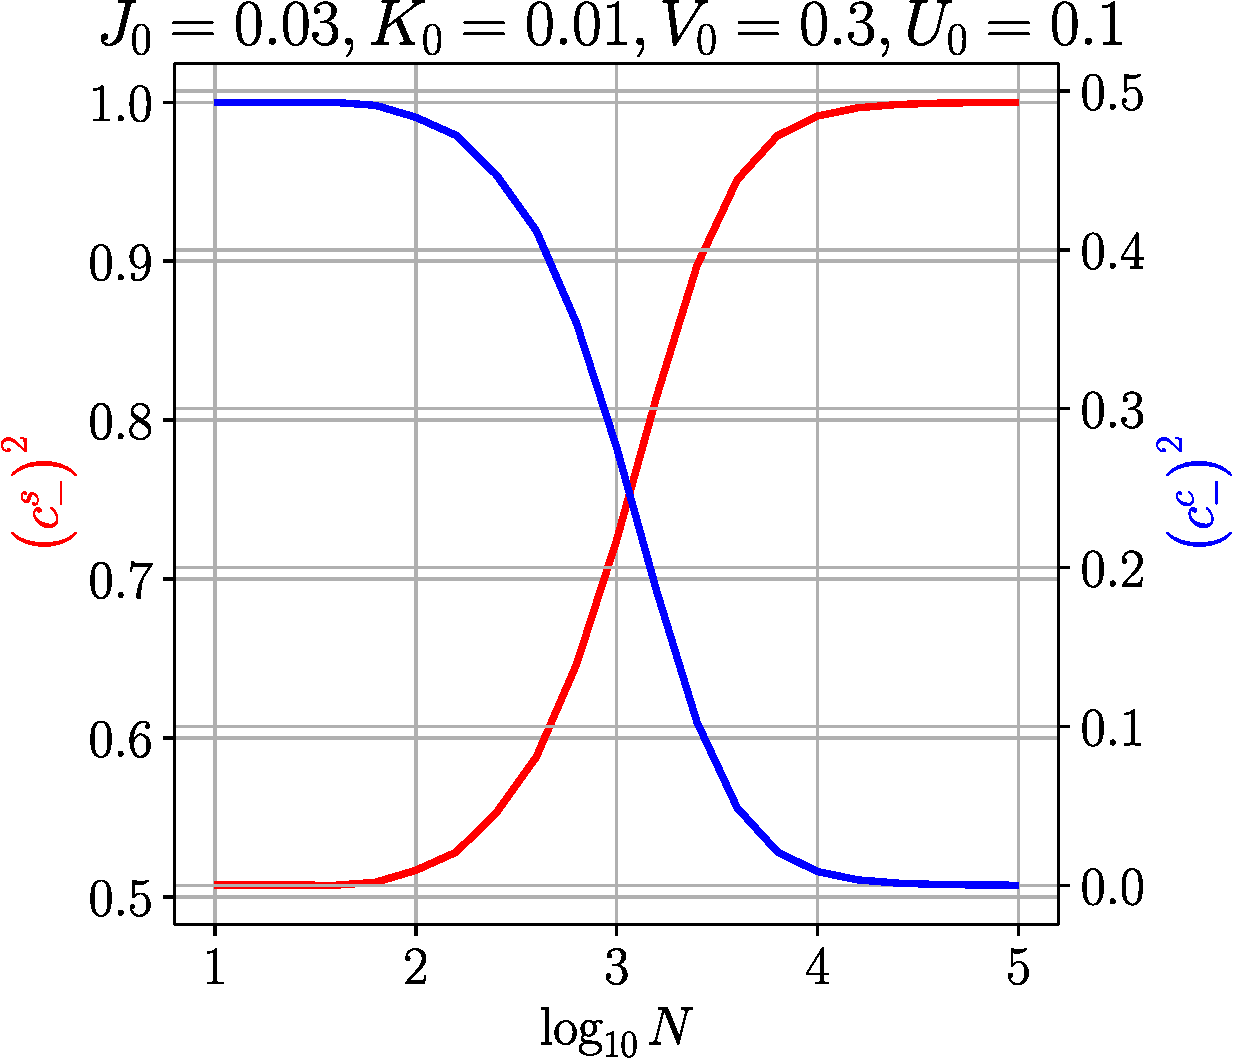
\includegraphics[width=0.52\textwidth]{../figures/cscc_q1.pdf}
	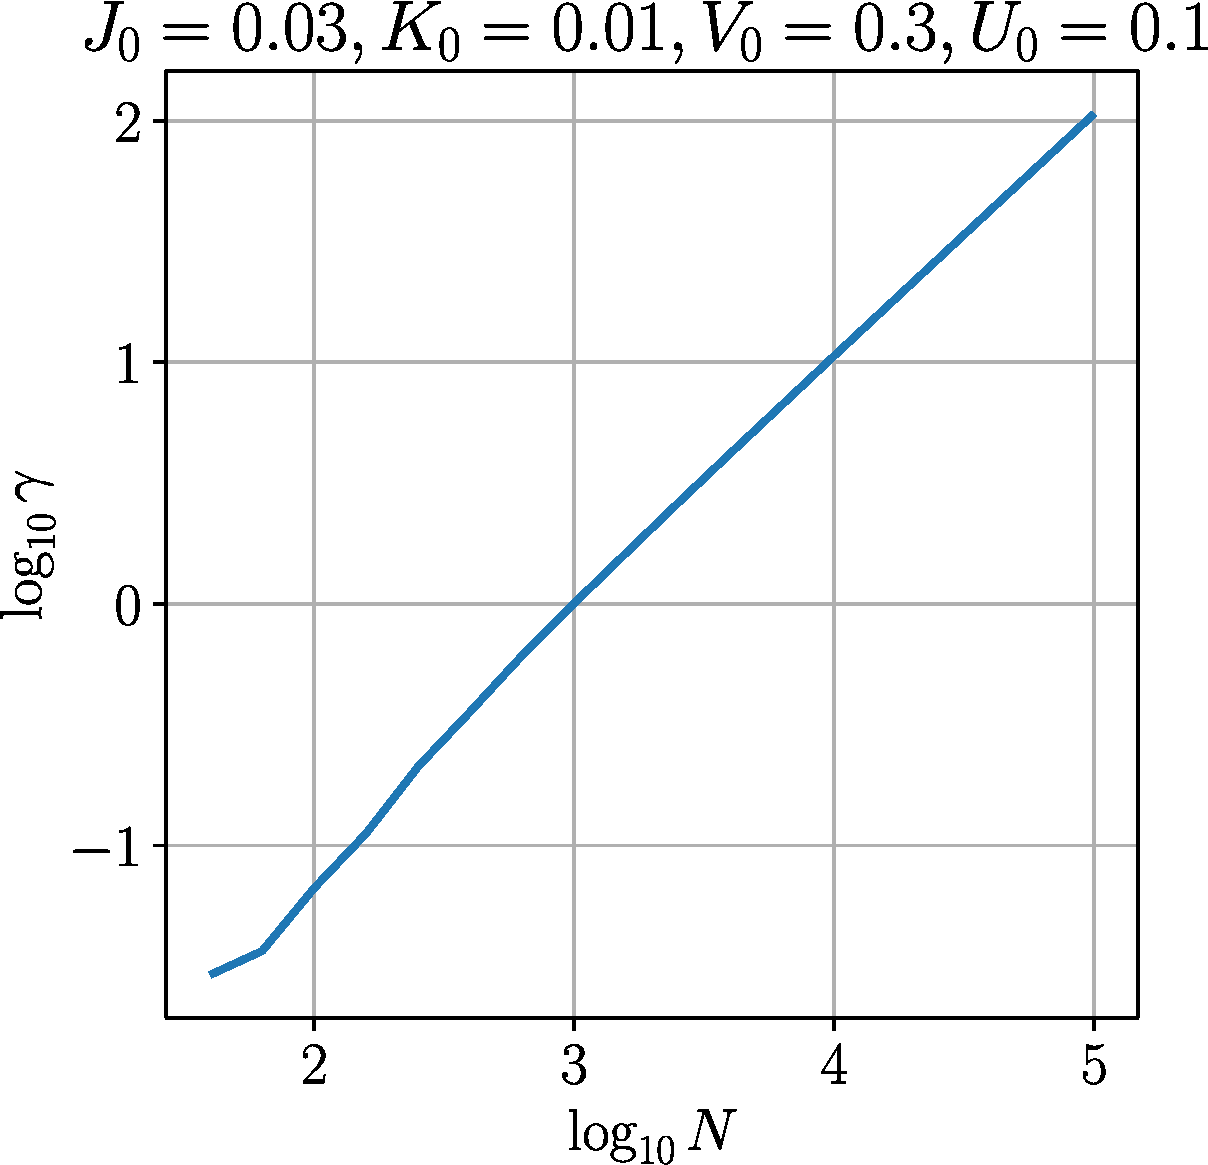
\includegraphics[width=0.46\textwidth]{../figures/gamma_q1.pdf}
	\caption{\textit{Left}: Variation of the probabilities \(\left(c^s\right)^2\) and \(\left(c^c\right)^2\) with system size. \textit{Right}: Variation of \(\gamma\) with system size.}
	\label{gamma}
\end{figure}
\\\\The full list of eigenstates is
\begin{table}[htpb!]
	\centering
	\begin{tabular}{|c|c|c|c|}
		\hline
		\(\hat n\) & \(S^z\) & eigenstate & eigenvalue\\
		\hline
		0 & 0 & \(\ket{0,0}\) & \(\frac{1}{4}k\)\\
		4 & 0 & \(\ket{2,2}\) & \(\frac{1}{4}k\)\\
		\multirow{2}{*}{1} & \(\frac{1}{2}\) & \(-4v\ket{\uparrow,0} +2 \left[ \epsilon_d \mp \Delta\left(\epsilon_d , v\right)\right] \ket{0, \uparrow}\) & \multirow{4}{*}{\(\frac{1}{2} \epsilon_d \pm \frac{1}{2}\Delta\left(\epsilon_d , v\right)\)}\\
		 & - \(\frac{1}{2}\) & \(-4v\ket{\downarrow,0} +2 \left[ \epsilon_d \mp \Delta\left(\epsilon_d , v\right)\right] \ket{0, \downarrow}\)  &\\
		\multirow{2}{*}{3} & \(\frac{1}{2}\) & \(-4v\ket{\uparrow,2} +2 \left[ \epsilon_d \mp \Delta\left(\epsilon_d , v\right)\right] \ket{2, \uparrow}\) &\\
		 & - \(\frac{1}{2}\) & \(-4v\ket{\downarrow,2} +2 \left[ \epsilon_d \mp \Delta\left(\epsilon_d , v\right)\right] \ket{2, \downarrow}\)  &\\
		\multirow{5}{*}{2} & 1,-1 & \(\ket{\uparrow,\uparrow}\), \(\ket{\downarrow,\downarrow}\) & \multirow{2}{*}{\(\epsilon_d + \frac{1}{4}j\)}\\
		& \multirow{3}{*}{0} & \(\ket{\uparrow,\downarrow} + \ket{\downarrow, \uparrow}\) & \\
		& & \(\ket{2,0} - \ket{0,2}\) & \(-\frac{3}{4}k\)\\
		& & \(c_\pm^s \frac{1}{\sqrt 2}\left(\ket{\uparrow, \downarrow} - \ket{\downarrow, \uparrow}\right) + c^c_\pm \frac{1}{\sqrt 2}\left(\ket{\uparrow\downarrow, 0} + \ket{0, \uparrow\downarrow}\right)\) & \(v\left[ \gamma \pm \sqrt{\gamma^2 + 4} \right] + \epsilon_d - \frac{3}{4}j\)\\
		\hline
	\end{tabular}
	\caption{Eigenstates for effective two-site Hamiltonian}
	\label{tab:label}
\end{table}
\\\\Although \(E^2_-\) is the ground state of this two-dimensional subspace, we haven't yet checked what is the true ground state of the full Hilbert space. The eigenstates eq.~\ref{1} through \ref{2} are obviously higher than \(E_-^2\), because of the presence of the singlet \(- \frac{3}{4}j\) and the negative \(\gamma\) contribution in \(E_-^2\) compared to the positive triplet contribution \( \frac{1}{4}j\) in those equations. The only other competitors are the one in eq.~\ref{hikari} which we call \(E_c^2\), and the low energy eigenstate in eq.~\ref{low}, which we call \(E_-^1\). We first shown that \(E_-^1 > E_-^2\). The difference between \(E_-^2\) and \(E_-^1\) is
\begin{equation}\begin{aligned}
	E_-^2 - E_-^1= - \frac{3}{4}\left( j + k \right) - \sqrt{4v^2 + \frac{\epsilon_d^2}{4} + \frac{9}{64}\left( j - k \right) ^2 - \frac{3}{8}\epsilon_d\left( j-k \right) } + \sqrt{ \frac{1}{4}\epsilon_d^2 + v^2}
\end{aligned}\end{equation}
From the nature of the fixed point phases, we know that 
\begin{equation}\begin{aligned}
	J^* > K^* \implies \epsilon_d^* \leq 0
\end{aligned}\end{equation}
and
\begin{equation}\begin{aligned}
	J^* < K^* \implies \epsilon_d^* \geq 0
\end{aligned}\end{equation}
such that
\begin{equation}\begin{aligned}
	\epsilon_d\left( j-k \right) \leq 0
\end{aligned}\end{equation}
This result then very easily implies that
\begin{equation}\begin{aligned}
	4v^2 + \frac{\epsilon_d^2}{4} + \frac{9}{64}\left( j - k \right) ^2 - \frac{3}{8}\epsilon_d\left( j-k \right) > \frac{1}{4}\epsilon_d^2 + v^2
\end{aligned}\end{equation}
and we can apply this inequality to the difference between \(E_-^2\) and \(E_-^1\) to see that \(E_-^2\) is greater that \(E_-^1\).
\\\\We now compare \(E_-^2\) and \(E_c^2\):
\begin{equation}\begin{aligned}
	\Delta E_g \equiv E_-^2 - E_c^2 = \frac{1}{2}\epsilon_d - \frac{3j + k}{8} + k - \sqrt{4v^2 + \left(\frac{3j+k}{8} -\frac{1}{2} \epsilon_d\right) ^2}
\end{aligned}\end{equation}
Because of the presence of the large \(v\) in the first quadrant, this will necessarily be negative there. So, the true ground state in the first quadrant is \(E_-^2\). In the third quadrant, the large value of \(k\) will make the difference positive and the true ground state will be the charge singlet. 
\\\\These conclusions have been checked numerically and shown in fig.~\ref{fig_gstate}, where we have plotted the sign of \(\Delta E_g\) as a function of \(K_0 - J_0\). For positive values of \(K_0 - J_0\), we are in the third quadrant, and the sign of \(\Delta E_g\) being \(+1\) implies that \(E_-^2 > E_c^2\), and so the third quadrant ground state is the charge singlet (\(E_c^2\)). On the other hand, as \(K_0 - J_0\) becomes negative, we move into the first quadrant, and the sign of \(\Delta E_g\) also flips, implying that we have a transition from the charge singlet to the (mostly) spin-singlet ground state.
\begin{figure}[htpb]
	\centering
	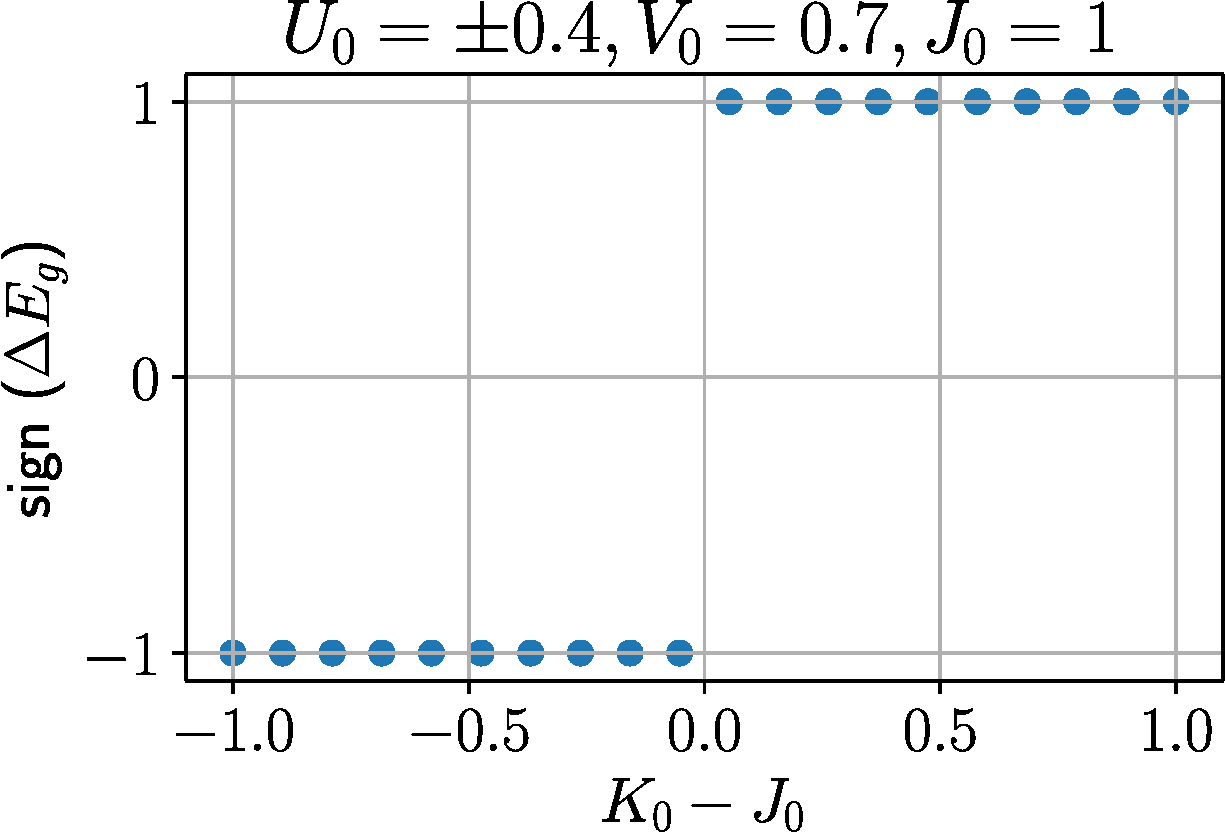
\includegraphics[width=0.5\textwidth]{../figures/gstate.pdf}
	\captionof{figure}{Shift of ground state in going from the first to third quadrant, depicted via the switch in sign of \(\Delta E_g\).}
	\label{fig_gstate}
\end{figure}
\\\\One of the most striking conclusions of this chapter is that the renormalized ground state of the SIAM in the Kondo regime is purely a singlet. The holon-doublon contributions of the ground state die out in the limit of large system size, and we are left purely with spin-sector contributions. This is, as far as we can see, due to two reasons: 
\begin{itemize}
	\item a higher RG flow rate of \(J\) as compared to \(V\)
	\item the fact that \(j \sim J N\) while \(v \sim V\sqrt N \)
\end{itemize}
These two factors help the s-d interaction term in becoming the most dominant term in the Hamiltonian, at the fixed point.

\section{Effective temperature scale at the fixed point}
We will first change the discrete RG equation to a continuum equation by interpreting \(\Delta J\) as \(\frac{\Delta J}{\Delta \ln D}\), where the denominator is unity: \(\Delta \ln D = 1\). Now, since the bandwidth is decreasing under the RG, we can write \(\Delta \ln D = -d \ln D\). The continuum equation (for \(K=0\)) becomes
\begin{equation}\begin{aligned}
	\frac{\:\mathrm{d}J}{\:\mathrm{d}\ln D} = n(0)J^2 \frac{1}{\omega - \frac{D}{2} + \frac{J}{4}}
\end{aligned}\end{equation}
where we have replaced by the number of states at each shell with that at the Fermi surface (uniform DOS). We can define a dimensionless quantity \(g \equiv \frac{J}{\frac{D}{2}} - \omega\). In terms of \(g\), the continuum RG equation becomes
\begin{equation}\begin{aligned}
	-\frac{\:\mathrm{d}g}{\:\mathrm{d}\ln D} + \frac{D g}{2\omega - D} = \frac{n(0) g^2}{1 - \frac{g}{4}}
\end{aligned}\end{equation}
Now, for the specific case where \(D\) is small (\(D \to 0\)), we can simplify and integrate this equation:
\begin{equation}\begin{aligned}
	\frac{\:\mathrm{d}g}{\:\mathrm{d}\ln D} &= \frac{n(0) g^2}{\frac{g}{4} - 1}\\
	\implies \left[\frac{1}{g} + \frac{1}{4}\ln g\right]_{g_0}^{g^*} &= n(0)\ln D\big\vert_{D_0}^{D^*}
\end{aligned}\end{equation}
\(g^*(_0), D^*(_0)\) are the fixed point (bare) values of \(g, D\). From the denominator structure, the fixed-point value is \(g^* =  4\). This gives an estimate of the bandwidth of the emergent window:
\begin{equation}\begin{aligned}
	D^* = D_0 \left( \frac{4}{g_0} \right)^\frac{1}{4n(0)}\exp\left\{-\frac{1}{n(0)}\left(\frac{1}{g_0} - \frac{1}{4}\right)\right\}
\end{aligned}\end{equation}
We can now define a temperature scale for the fixed-point theory:
\begin{equation}\begin{aligned}
	T_K \equiv \frac{2N^*}{\pi}D^* = \frac{2N^*}{\pi}D_0 \left( \frac{4}{g_0} \right)^\frac{1}{4n(0)}\exp\left\{-\frac{1}{n(0)}\left(\frac{1}{g_0} - \frac{1}{4}\right)\right\}
\end{aligned}\end{equation}
The factor of \(2N^*\) is inserted to make the Kondo temperature intensive (we will see below that the \(N^*\) allows it to  be written in terms of parameters of the two-site Hamiltonian) - \(2N^*\) is the total number of momentum states in the fixed point theory. The factor of \(\frac{1}{\pi}\) is for aesthetic reasons. Since we have and will primarily work with \(\omega=0\), the fixed point condition can be used to write \(D^* = \frac{J^* + K^*}{2}\).
\begin{equation}\begin{aligned}
	T_K = \frac{2N^*}{\pi}\frac{1}{2}\left(J^* + K^*\right) = \frac{1}{\pi}\left(j + k\right)
\end{aligned}\end{equation}

\chapter{Results and Features of the Low-Energy Theory}
\label{results}
\section{Magnetic susceptibility}
The thermal susceptibility is defined as
\begin{equation}\begin{aligned}
	\label{chi_def}
	\chi(\beta) = \beta \left(\left<\left(S_d^z\right)^2\right> - \left<S_d^z\right>^2\right)
\end{aligned}\end{equation}
There is an alternate way of calculating this. We insert a fictitious magnetic field that couples only to the impurity site. The Hamiltonian in the presence of this field is
\begin{equation}\begin{aligned}
	\mathcal{H}^\prime(B) = \mathcal{H} + B S_d^z
\end{aligned}\end{equation}
The susceptibility is then given by
\begin{equation}\begin{aligned}
	\label{chi_exp}
	\chi(\beta) &= \lim_{B \to 0}\frac{1}{\beta}\left[\frac{1}{Z(B)} \frac{\partial^2{Z(B)}}{\partial{B^2}}-\frac{1}{Z(B)^2} \left(\frac{\partial{Z(B)}}{\partial{B}}\right)^2\right]
\end{aligned}\end{equation}
where \(Z(B)\) is the partition function of the Hamiltonian \(\mathcal{H}^\prime(B)\). The following is to prove that the RHS of eqs.~\ref{chi_def} and \ref{chi_exp} are the same. We start with \ref{chi_exp}. The first derivative can be written as
\begin{equation}\begin{aligned}
	\frac{\partial{Z(B)}}{\partial{B}} = \text{Trace}\left[\frac{\partial{}}{\partial{B}} \exp\left\{-\beta\left( \mathcal{H} + BS_d^z \right) \right\}\right] = \text{Trace}\left[-\beta S_d^z \exp\left\{-\beta\left( \mathcal{H} + BS_d^z \right) \right\}\right]
\end{aligned}\end{equation}
which means the first term becomes
\begin{equation}\begin{aligned}
	\lim_{B \to 0}-\frac{1}{Z(B)^2} \left(\frac{\partial{Z(B)}}{\partial{B}}\right)^2 = -\left(\beta \frac{1}{\text{Trace}\left[\exp\left\{-\beta\mathcal{H}\right\}\right]} \text{Trace}\left[S_d^z \exp\left\{-\beta\mathcal{H}\right\}\right]\right)^2 = -\beta^2 \left<S_d^z\right>^2
\end{aligned}\end{equation}
The second derivative is
\begin{equation}\begin{aligned}
	\frac{\partial^2{Z(B)}}{\partial{B^2}} = \text{Trace}\left[-\beta S_d^z  \frac{\partial{}}{\partial{B}}\exp\left\{-\beta \left( \mathcal{H} + BS_d^z \right) \right\}\right] = \text{Trace}\left[\beta^2 \left(S_d^z\right)^2 \exp\left\{-\beta \left( \mathcal{H} + BS_d^z \right) \right\}\right]
\end{aligned}\end{equation}
so the second term becomes
\begin{equation}\begin{aligned}
	\lim_{B \to 0}\frac{1}{Z(B)} \frac{\partial^2{Z(B)}}{\partial{B^2}} = \beta^2 \frac{1}{\text{Trace}\left[\exp\left\{-\beta \mathcal{H}\right\}\right]}\text{Trace}\left[\left(S_d^z\right)^2 \exp\left\{-\beta \mathcal{H}\right\}\right] = \beta^2 \left<\left(S_d^z\right)^2 \right>
\end{aligned}\end{equation}
The full thing becomes
\begin{equation}\begin{aligned}
	\lim_{B \to 0}\frac{1}{\beta}\left[\frac{1}{Z(B)} \frac{\partial^2{Z(B)}}{\partial{B^2}}-\frac{1}{Z(B)^2} \left(\frac{\partial{Z(B)}}{\partial{B}}\right)^2\right] = \frac{1}{\beta}\left(-\beta^2 \left<S_d^z\right>^2 + \beta^2 \left<\left(S_d^z\right)^2 \right>\right) \\
	= \beta \left(\left<\left(S_d^z\right)^2\right> - \left<S_d^z\right>^2\right) 
\end{aligned}\end{equation}
This completes the proof. 
\subsection{For \(v=0\)}
In the presence of a magnetic field coupling term \(B S^z_1\), the eigenvalues become (setting \(v = 0\))
\begin{equation}\begin{aligned}
\hat n=0,4 &\rightarrow E^0 = \frac{1}{4}k\\
\hat n=1,3 &\rightarrow \begin{cases}
	E^1_{\pm, \uparrow} = \frac{1}{2} \left(\epsilon_d + \frac{1}{2}B\right) \pm \frac{1}{2}\Delta\left(\epsilon_d + \frac{1}{2}B, v\right)  = \epsilon_d + \frac{1}{2}B, 0\\ 
	E^1_{\pm, \downarrow} = \frac{1}{2} \left(\epsilon_d - \frac{1}{2}B\right) \pm \frac{1}{2}\Delta\left(\epsilon_d - \frac{1}{2}B, v\right)  = \epsilon_d -\frac{1}{2}B, 0
	\end{cases}\\
	\hat n=2 &\rightarrow \begin{cases}
	\epsilon_d + \frac{1}{4}j + \frac{1}{2}B\\
	\epsilon_d + \frac{1}{4}j - \frac{1}{2}B\\
	\frac{1}{4}k \\
	-\frac{3}{4}k \\
	\epsilon_d -\frac{1}{4}j \pm \frac{1}{2} \Gamma \\
\end{cases}
\end{aligned}\end{equation}
where we defined \(\Gamma = \sqrt{B^2 + j^2}\). The eigenvalues in \(\hat n=2\) can be elaborated upon. The action of the total Hamiltonian \(\mathcal{H}^\prime\) (with \(v=0\)) is
\begin{flalign}
	\ket{\uparrow, \uparrow} &\mapsto \left(\epsilon_d + \frac{1}{4}j + \frac{1}{2}B\right)\ket{\uparrow, \uparrow}\\
	\ket{\downarrow, \downarrow} &\mapsto \left(\epsilon_d + \frac{1}{4}j - \frac{1}{2}B\right)\ket{\downarrow, \downarrow}\\
	\frac{1}{\sqrt 2}\left(\ket{\uparrow\downarrow, 0} + \ket{0, \uparrow\downarrow}\right) &\mapsto \frac{1}{4}k\frac{1}{\sqrt 2}\left(\ket{\uparrow\downarrow, 0} + \ket{0, \uparrow\downarrow}\right)\\
	\frac{1}{\sqrt 2}\left(\ket{\uparrow\downarrow, 0} - \ket{0, \uparrow\downarrow}\right) &\mapsto - \frac{3}{4}k \frac{1}{\sqrt 2}\left(\ket{\uparrow\downarrow, 0} - \ket{0, \uparrow\downarrow}\right)\\
	\frac{1}{\sqrt 2}\left(\ket{\uparrow, \downarrow} + \ket{\downarrow, \uparrow}\right) &\mapsto \left( \epsilon_d + \frac{1}{4}j \right) \frac{1}{\sqrt 2}\left(\ket{\uparrow, \downarrow} + \ket{\downarrow, \uparrow}\right) + \frac{1}{2}B\frac{1}{\sqrt 2}\left(\ket{\uparrow, \downarrow} - \ket{\downarrow, \uparrow}\right)\\
	\frac{1}{\sqrt 2}\left(\ket{\uparrow, \downarrow} - \ket{\downarrow, \uparrow}\right) &\mapsto \left( \epsilon_d - \frac{3}{4}j \right) \frac{1}{\sqrt 2}\left(\ket{\uparrow, \downarrow} - \ket{\downarrow, \uparrow}\right) + \frac{1}{2}B \frac{1}{\sqrt 2}\left(\ket{\uparrow, \downarrow} + \ket{\downarrow, \uparrow}\right)\\
\end{flalign}
The first four states directly give the first four eigenvalues in \(\hat n=2\). The remaining two states form the matrix
\begin{equation}\begin{aligned}
	\begin{pmatrix} \epsilon_d + \frac{1}{4}j & \frac{1}{2}B \\ \frac{1}{2}B & \epsilon_d - \frac{3}{4}j \end{pmatrix} 
\end{aligned}\end{equation}
The eigenvalues satisfy the equation
\begin{equation}\begin{aligned}
	0 = \left( E - \epsilon_d + \frac{3}{4}j \right) \left( E - \epsilon_d - \frac{1}{4}j \right) - \frac{1}{4}B^2 = \left( E - \epsilon_d - \frac{1}{4}j \right) ^2 + j \left( E - \epsilon_d - \frac{1}{4}j \right) - \frac{1}{4}B^2
\end{aligned}\end{equation}
The solutions are
\begin{equation}\begin{aligned}
	E = \epsilon_d + \frac{1}{4}j + \frac{-j \pm \sqrt{j^2 + B^2}}{2} = \epsilon_d - \frac{1}{4}j \pm \frac{1}{2}\Gamma
\end{aligned}\end{equation}
which are the final two eigenvalues.
\\\\The partition function is
\begin{equation}\begin{aligned}
	Z(B) &= 2 \exp\left\{-\beta \frac{k}{4}\right\} + 2\left( \exp\left\{-\beta\left(\epsilon_d + \frac{1}{2} B\right)\right\} + e^0\right) + 2\left( \exp\left\{-\beta\left(\epsilon_d - \frac{1}{2} B\right)\right\} + e^0\right) \\
	     &+ \exp\left\{-\beta\left(\epsilon_d + \frac{1}{4}j + \frac{1}{2} B\right)\right\} + \exp\left\{-\beta\left(\epsilon_d + \frac{1}{4}j - \frac{1}{2} B\right)\right\} \\
	     &+ \exp\left\{-\beta \frac{k}{4}\right\} + \exp\left\{\beta \frac{3k}{4}\right\} + \exp\left\{-\beta\left(\epsilon_d - \frac{1}{4}j + \frac{1}{2}\Gamma\right)\right\} + \exp\left\{-\beta\left( \epsilon_d- \frac{1}{4}j - \frac{1}{2}\Gamma\right)\right\}\\
	     &= 4 + 3\exp\left\{-\beta \frac{k}{4}\right\} + \exp\left\{\beta \frac{3k}{4}\right\} + 4e^{-\beta \epsilon_d}\cosh \beta \frac{B}{2} + 2e^{-\beta \left(\epsilon_d + \frac{j}{4}\right)}\cosh \beta \frac{B}{2}\\
	     &+ 2e^{-\beta\left(\epsilon_d - \frac{j}{4}\right)}\cosh \beta \frac{1}{2}\Gamma\\
	     &= 4 + 3\exp\left\{-\beta \frac{k}{4}\right\} + \exp\left\{\beta \frac{3k}{4}\right\} + \left[4e^{-\beta \epsilon_d} + 2e^{-\beta \left(\epsilon_d + \frac{j}{4}\right)}\right]\cosh \left(\beta \frac{B}{2}\right) \\
	     &+ 2e^{-\beta\left(\epsilon_d - \frac{j}{4}\right)}\cosh \left(\beta \frac{1}{2}\Gamma\right)
\end{aligned}\end{equation}
We can now compute the derivatives.
\begin{equation}\begin{aligned}
	Z^\prime \equiv \frac{\partial{Z}}{\partial{B}} =& \left[4e^{-\beta \epsilon_d} + 2e^{-\beta \left(\epsilon_d + \frac{j}{4}\right)}\right] \frac{\beta}{2}\sinh \left(\beta \frac{B}{2}\right) + 2e^{-\beta\left(\epsilon_d - \frac{j}{4}\right)}\frac{1}{2}\beta \sinh \left(\frac{1}{2}\beta \Gamma\right) \frac{\partial{\Gamma}}{\partial{B}} \\
	=& \left[4e^{-\beta \epsilon_d} + 2e^{-\beta \left(\epsilon_d + \frac{j}{4}\right)}\right] \frac{\beta}{2}\sinh \left(\beta \frac{B}{2}\right) + e^{-\beta\left(\epsilon_d - \frac{j}{4}\right)}\beta \sinh \left(\frac{1}{2}\beta \Gamma \right) \frac{B}{\Gamma}\\
	Z^{\prime\prime} \equiv \frac{\partial^2{Z}}{\partial{B^2}} =& \left[4e^{-\beta \epsilon_d} + 2e^{-\beta \left(\epsilon_d + \frac{j}{4}\right)}\right] \left(\frac{\beta}{2}\right)^2 \cosh \left(\beta \frac{B}{2}\right) \\
								     &+ e^{-\beta\left(\epsilon_d - \frac{j}{4}\right)}\beta \left[\cosh \left(\frac{1}{2}\beta \Gamma \right) \times \frac{1}{2}\beta \left(\frac{B}{\Gamma}\right)^2 + \sinh \left(\frac{1}{2}\beta \Gamma \right) \left(-\frac{B}{\Gamma^2}\times \frac{B}{\Gamma} + \frac{1}{\Gamma} \right)\right]
\end{aligned}\end{equation}
Taking the limit of \(B \to 0\) gives
\begin{equation}\begin{aligned}
	Z\vert_{B=0} &= 4 + 3\exp\left\{-\beta \frac{k}{4}\right\} + \exp\left\{\beta \frac{3k}{4}\right\} + 4e^{-\beta \epsilon_d} + 2e^{-\beta \left(\epsilon_d + \frac{j}{4}\right)} + 2e^{-\beta\left(\epsilon_d - \frac{j}{4}\right)}\cosh \left(\beta \frac{j}{2}\right)\\
	Z^\prime\vert_{B=0} &= 0\\
	Z^{\prime\prime}\vert_{B=0} &= \left[4e^{-\beta \epsilon_d} + 2e^{-\beta \left(\epsilon_d + \frac{j}{4}\right)}\right] \left(\frac{\beta}{2}\right)^2 + e^{-\beta\left(\epsilon_d - \frac{j}{4}\right)}\beta \sinh \left(\beta \frac{j}{2} \right) \frac{1}{j}\\
\end{aligned}\end{equation}
The susceptibility is thus
\begin{equation}\begin{aligned}
	\chi(\beta) &= \frac{1}{\beta}\frac{\left[4e^{-\beta \epsilon_d} + 2e^{-\beta \left(\epsilon_d + \frac{j}{4}\right)}\right] \left(\frac{\beta}{2}\right)^2 + e^{-\beta\left(\epsilon_d - \frac{j}{4}\right)}\beta \sinh \left(\beta \frac{j}{2} \right) \frac{1}{j}}{4 + 3\exp\left\{-\beta \frac{k}{4}\right\} + \exp\left\{\beta \frac{3k}{4}\right\} + 4e^{-\beta \epsilon_d} + 2e^{-\beta \left(\epsilon_d + \frac{j}{4}\right)} + 2e^{-\beta\left(\epsilon_d - \frac{j}{4}\right)}\cosh \left(\beta \frac{j}{2}\right)}\\
		    &=\frac{\left[2e^{-\beta \epsilon_d} + e^{-\beta \left(\epsilon_d + \frac{j}{4}\right)}\right] \frac{1}{2}\beta + e^{-\beta\left(\epsilon_d - \frac{j}{4}\right)} \sinh \left(\beta \frac{j}{2} \right) \frac{1}{j}}{4 + 3\exp\left\{-\beta \frac{k}{4}\right\} + \exp\left\{\beta \frac{3k}{4}\right\} + 4e^{-\beta \epsilon_d} + 2e^{-\beta \left(\epsilon_d + \frac{j}{4}\right)} + 2e^{-\beta\left(\epsilon_d - \frac{j}{4}\right)}\cosh \left(\beta \frac{j}{2}\right)}\\
\end{aligned}\end{equation}
At high temperatures, we can write
\begin{equation}\begin{aligned}
	\frac{\chi}{\beta}\vert_{\beta \to 0} = \frac{\left[4 + 2\right] \frac{1}{4} + \frac{1}{2}\lim_{\beta \to 0}\sinh \left(\beta \frac{j}{2} \right) \frac{2}{\beta j}}{4 + 3 + 1 + \left[4 + 2\right] + 2} = \frac{\frac{3}{2} + \frac{1}{2}}{16} = \frac{1}{8} && \left[\lim_{x \to 0} \frac{\sinh x}{x} = 1\right] \\
\end{aligned}\end{equation}
At low temperatures,
\begin{equation}\begin{aligned}
	\chi\vert_{\beta \to \infty} = \lim_{\beta \to \infty} \frac{e^{-\beta\left(\epsilon_d - \frac{j}{4}\right)} \sinh \left(\beta \frac{j}{2} \right) \frac{1}{j}}{\exp\left\{\beta \frac{3k}{4}\right\} + 2e^{-\beta\left(\epsilon_d - \frac{j}{4}\right)}\cosh \left(\beta \frac{j}{2}\right)} =  \frac{1}{2j}\lim_{\beta \to \infty} \frac{1}{\exp\left\{\beta \left(\frac{3k}{4} + \epsilon_d - \frac{3j}{4}\right)\right\} + 1} \\
\end{aligned}\end{equation}
There we used \(\sinh x \approx \cosh x \approx \frac{1}{2}e^x \text{ for }x\to \infty\). The exponential will take the following limiting values:
\begin{equation}\begin{aligned}
	\exp\left\{\beta \left(\frac{3k}{4} + \epsilon_d - \frac{3j}{4}\right)\right\} \to \begin{cases}
		\infty, & \text{ if } \frac{3k}{4} + \epsilon_d - \frac{3j}{4} > 0\\
		1, & \text{ if } \frac{3k}{4} + \epsilon_d - \frac{3j}{4} = 0\\
		0, & \text{ if } \frac{3k}{4} + \epsilon_d - \frac{3j}{4} < 0
	\end{cases}
\end{aligned}\end{equation}
which means
\begin{equation}\begin{aligned}
	\left[\exp\left\{\beta \left(\frac{3k}{4} + \epsilon_d - \frac{3j}{4}\right)\right\} + 1\right]^{-1} \to \begin{cases}
		0, & \text{ if } \frac{3k}{4} + \epsilon_d - \frac{3j}{4} > 0\\
		\frac{1}{2}, & \text{ if } \frac{3k}{4} + \epsilon_d - \frac{3j}{4} = 0\\
		1, & \text{ if } \frac{3k}{4} + \epsilon_d - \frac{3j}{4} < 0
	\end{cases} = \Theta\left(\frac{3j}{4} - \frac{3k}{4} - \epsilon_d\right) 
\end{aligned}\end{equation}
where the theta function (Heaviside function) is defined as 
\begin{equation}\begin{aligned}
	\Theta(x) = \begin{cases}
		1, & \text{ if }x>0\\
		\frac{1}{2}, & \text{ if }x=0\\
		0, & \text{ if }x<0\\
	\end{cases}
\end{aligned}\end{equation}
The thermal susceptibility at high temperatures is thus
\begin{equation}\begin{aligned}
	\chi\vert_{\beta \to \infty} = \frac{1}{2j}\Theta\left(\frac{3j}{4} - \frac{3k}{4} - \epsilon_d\right) 
\end{aligned}\end{equation}
If we are in the first quadrant, then the fixed point values are such that \(\frac{3k}{4} + \epsilon_d - \frac{3j}{4} < 0\), so the theta function will evaluate to 1, and we can write
\begin{equation}\begin{aligned}
	\chi\vert_{\beta \to \infty} = \frac{1}{2j}
\end{aligned}\end{equation}
For sufficiently large values of \(j\) compared to \(k\), we can also approximate the Kondo temperature \(T_K\) as \(T_K \approx \frac{j}{\pi}\). Then, the zero temperature value of \(\chi\) deep in the first quadrant is
\begin{equation}\begin{aligned}
	\chi(T = 0) \approx \left(2 \pi T_K\right)^{-1}
\end{aligned}\end{equation}
This is in accordance with the results obtained from Bethe ansatz in \cite{okiji_kawakami}. The variation of \(\chi \times T\) and \(\left(T_K \chi\right)^{-1}\) against temperature is shown in fig.~\ref{sus_spin}.
\\\\On the other hand, in the third quadrant, we have \(\frac{3k}{4} + \epsilon_d - \frac{3j}{4} > 0\), and \(\Theta\) gives
\begin{equation}\begin{aligned}
	\chi\vert_{\beta \to \infty} = 0
\end{aligned}\end{equation}
The variation of \(\chi\) against \(T\) is shown in fig.~\ref{sus_T}. The susceptibility goes through a maximum at a certain temperature, and this maximum is not present in NRG or Bethe Ansatz calculations. We suspect that this peak is an artifact of the simplification suffered in restricting the calculation to just the zero mode of the conduction bath. We intend to investigate this by allowing for higher modes of the bath. The speculation that this is due to the zero mode is further strengthened by the fact that a similar maximum was observed in the Kondo model susceptibility as obtained from a URG treatment and zero-mode effective Hamiltonian, in \cite{am_thesis}.
\begin{figure}[htpb!]
	\centering
	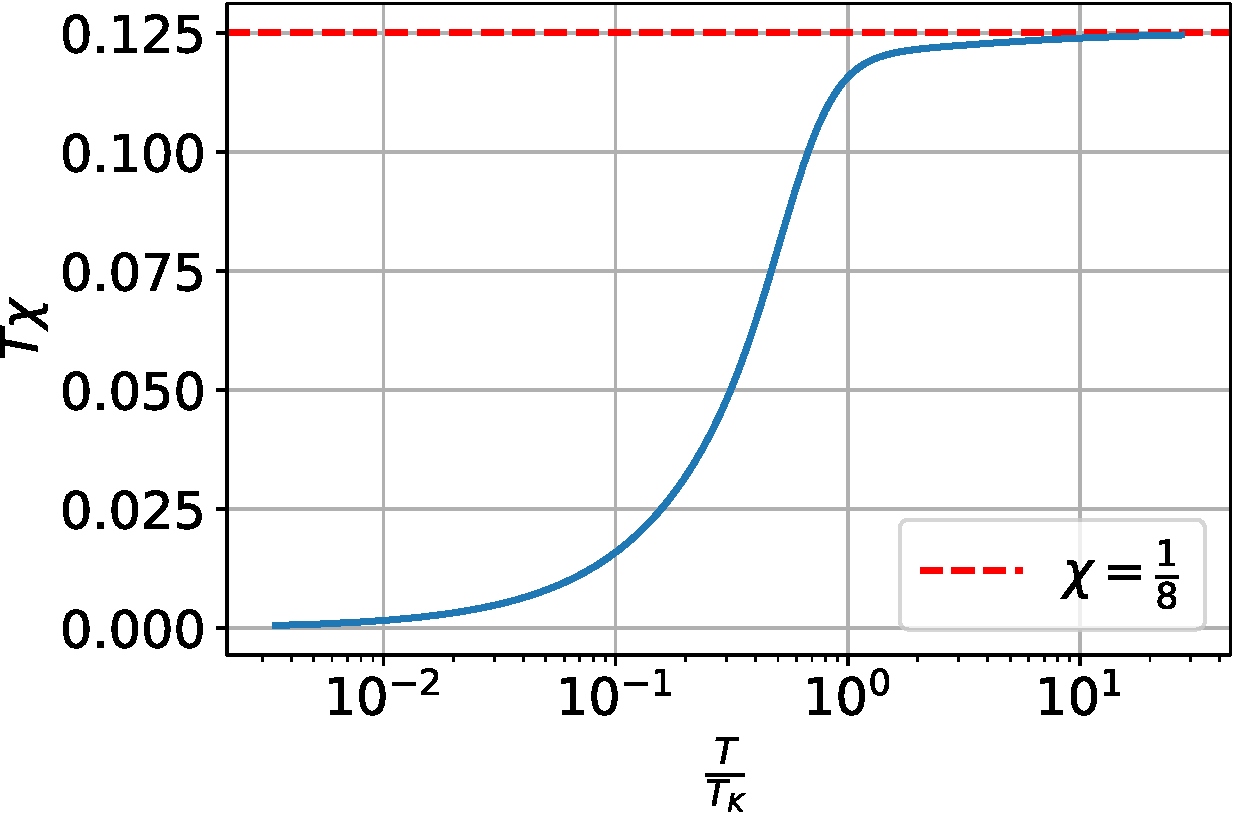
\includegraphics[width=0.49\textwidth]{../figures/chi_T_new.pdf}
	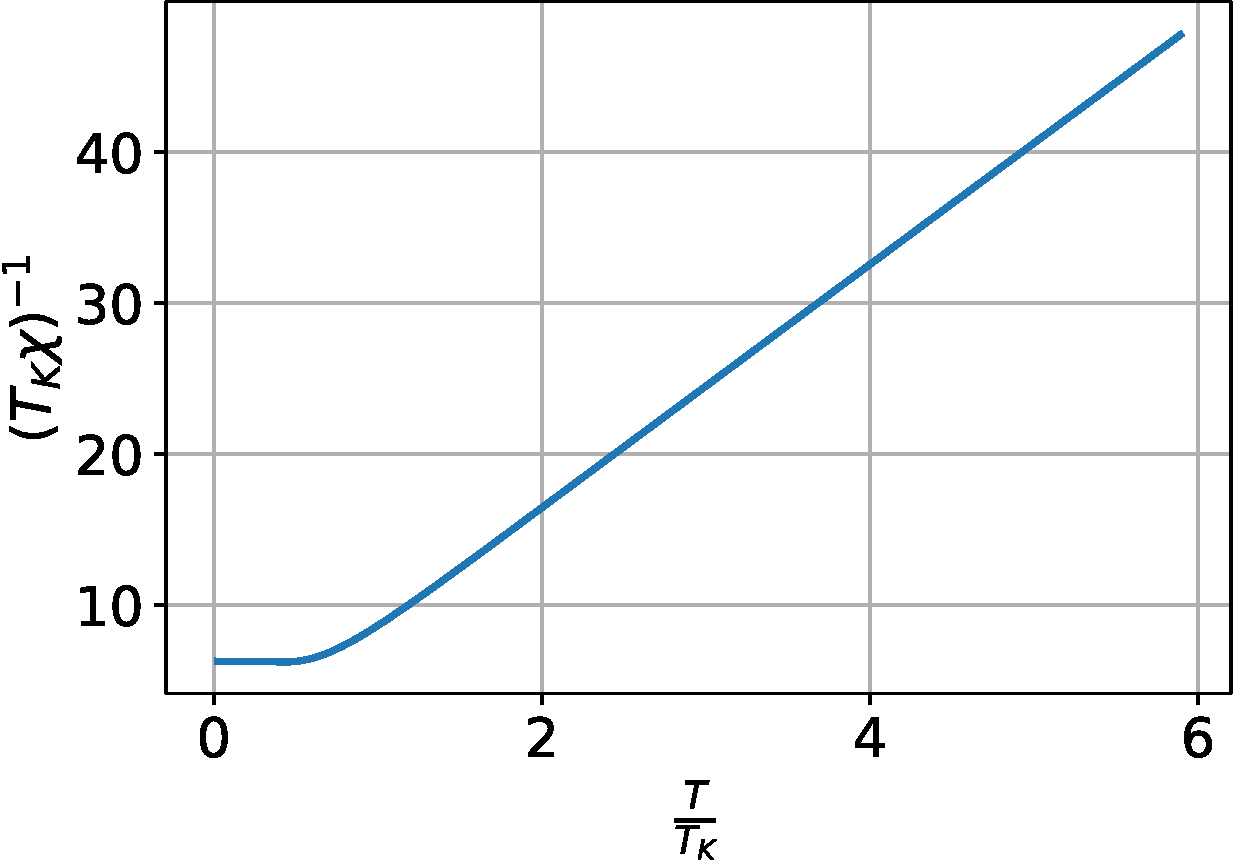
\includegraphics[width=0.49\textwidth]{../figures/one_over_chi_new.pdf}
	\caption{\textit{Left}:Variation of $\chi \times T$ over six decades of temperature. The low temperature behavior is characteristic of a local Fermi liquid paramagnetic susceptibility, while at high temperatures we see the Curie-Weiss susceptibility resulting from the local moment. \textit{Right}:Variation of \(\left(T_k \times \chi\right)^{-1}\) with temperature.}
	\label{sus_spin}
\end{figure}
\begin{figure}[htpb]
	\centering
	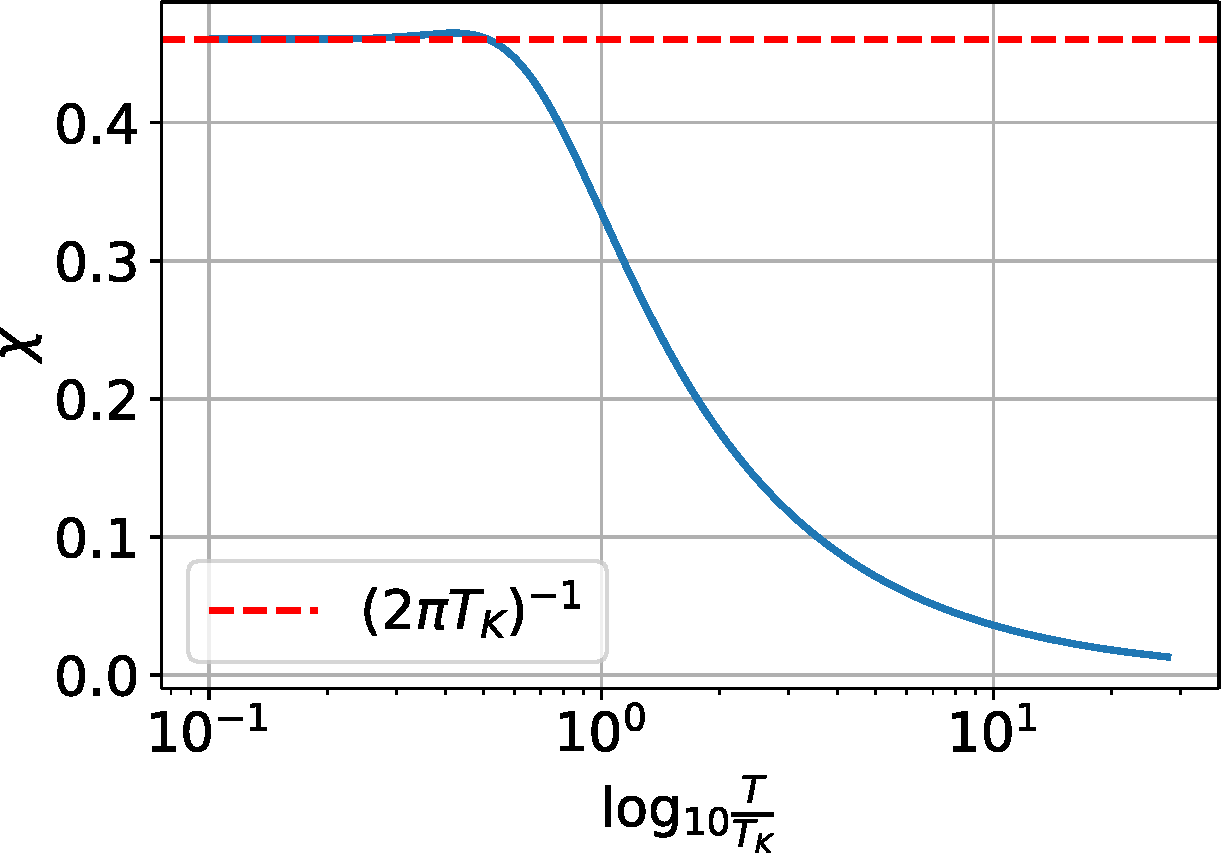
\includegraphics[width=0.6\textwidth]{../figures/chi_new.pdf}
	\caption{Variation of $\chi$ against temperature. It saturates to a value close to \(\left( 2\pi T_K \right) ^{-1}\)}
	\label{sus_T}
\end{figure}

\section{Charge Susceptibility}
We can also calculate the impurity contribution to the charge susceptibility of the system in a very similar fashion. We insert a magnetic field that couples to the impurity charge isospin:
\begin{equation}\begin{aligned}
	\mathcal{H}^\prime(B) = \mathcal{H} + B C_d^z
\end{aligned}\end{equation}
We again work in the simpler case of \(v=0\). The energy eigenvalues for this Hamiltonian are
\begin{equation}\begin{aligned}
\hat n=0 & \rightarrow\frac{1}{4}k - \frac{B}{2}\\
\hat n=4 &\rightarrow\frac{1}{4}k + \frac{B}{2}\\
\hat n=1,3 &\rightarrow \begin{cases}
	\epsilon_d - \frac{1}{2}B, 0\\ 
	\epsilon_d + \frac{1}{2}B, 0
	\end{cases}\\
	\hat n=2 &\rightarrow \begin{cases}
	\left.\epsilon_d + \frac{1}{4}j \right\}\times 3\\
	\epsilon_d - \frac{3}{4}j \\
	\epsilon_d -\frac{1}{4}k \pm \frac{1}{2} \Gamma \\
\end{cases}
\end{aligned}\end{equation}
where \(\Gamma \equiv \sqrt{k^2 + B^2}\). We will again use eq.~\ref{chi_exp} to calculate the susceptibility. The partition function and its derivatives are
\begin{equation}\begin{aligned}
	\lim_{B \to 0} Z &= 2e^{-\beta \frac{k}{4}} + 4 + 4e^{-\beta \epsilon_d} + 3e^{-\beta\left( \epsilon_d + \frac{j}{4} \right) } + e^{\beta\left( 3\frac{j}{4} - \epsilon_d \right)} + 2e^{\beta \left(\frac{k}{4} - \epsilon_d\right)}\cosh \beta \frac{k}{2}\\
	\lim_{B \to 0} \frac{\partial{Z}}{\partial{B}} &= 0 \\
	\lim_{B \to 0} \frac{\partial{^2Z}}{\partial{B^2}} &= \frac{\beta^2}{2}\left[e^{-\beta \frac{k}{4}} + 2e^{-\beta \epsilon_d}\right] + \frac{\beta}{k}e^{\beta\left(\frac{k}{4} - \epsilon_d\right)}\sinh \beta\frac{k}{2}
\end{aligned}\end{equation}
The charge susceptibility is thus
\begin{equation}\begin{aligned}
	\chi_c = \frac{1}{\beta}\frac{\frac{\beta^2}{2}\left[e^{-\beta \frac{k}{4}} + 2e^{-\beta \epsilon_d}\right] + \frac{\beta}{k}e^{\beta\left(\frac{k}{4} - \epsilon_d\right)}\sinh \beta\frac{k}{2}}{2e^{-\beta \frac{k}{4}} + 4 + 4e^{-\beta \epsilon_d} + 3e^{-\beta\left( \epsilon_d + \frac{j}{4} \right) } + e^{\beta\left( 3\frac{j}{4} - \epsilon_d \right)} + 2e^{\beta \left(\frac{k}{4} - \epsilon_d\right)}\cosh \beta \frac{k}{2}}
\end{aligned}\end{equation}
This is plotted in fig.~\ref{charge_sus}. The charge susceptibility at large temperatures becomes
\begin{equation}\begin{aligned}
	\left(\chi_c\times T\right) (T \to \infty) = \frac{1}{8}
\end{aligned}\end{equation}
The variation of \(\chi_c \times T\) and \(\chi_c^{-1}\) against temperature is also shown in figs.~\ref{chcT},\ref{one_over_chic}.
\\\\An important result that we will use later is the value at \(T=0\).
\begin{equation}\begin{aligned}
	\chi_c(T=0) =  \frac{1}{2k}\lim_{\beta \to \infty} \frac{1}{1 + e^{\frac{3\beta}{4} \left(j-k\right) }}
\end{aligned}\end{equation}
There we used the observation that near the fixed point, \(\epsilon_d\) is either close to zero or large positive such that \(e^{-\beta \epsilon_d}\) does not affect the value of \(\chi_c\) at \(T=0\). In the Kondo regime of the SIAM \((j \gg k)\), the denominator diverges and the charge susceptibility vanishes at \(T=0\). This is shown in fig.~\ref{chi_c_zero}.
\begin{equation}\begin{aligned}
	\chi_c(T=0)\bigg\vert_{j \gg k} = 0
\end{aligned}\end{equation}
\begin{figure}[htpb]
	\centering
	\includegraphics[height=0.27\textheight]{../figures/chi_c_new.pdf}
	\caption{Variation of \(\chi_c\) over 5 decades of temperature, for the charge-Kondo regime. Similar to the spin susceptibility, it saturates to \(\left( 2\pi T_K \right)^{-1}\).}
	\label{charge_sus}
\end{figure}
\begin{figure}[htpb]
	\centering
	\includegraphics[height=0.27\textheight]{../figures/T_chi_c_new.pdf}
	\caption{Behavior of \(\chi_c\times T\) for the charge-Kondo regime. It is qualitatively very similar to the behavior of the magnetic susceptibility in the spin-Kondo regime.}
	\label{chcT}
\end{figure}
\begin{figure}[htpb]
	\centering
	\includegraphics[height=0.27\textheight]{../figures/one_over_chi_c_new.pdf}
	\caption{Behavior of \(\left(T_K \chi_c\right)^{-1}\) for the charge-Kondo regime.}
	\label{one_over_chic}
\end{figure}
\begin{figure}[htpb]
	\centering
	\includegraphics[width=0.4\textheight]{../figures/chi_c_zero_new.pdf}
	\caption{Flow of charge susceptibility to 0 at low temperatures for the spin-Kondo regime (\(J>K\)).}
	\label{chi_c_zero}
\end{figure}

\section{Specific heat}
The specific heat is calculated by diagonalizing the fixed point Hamiltonian, numerically. The obtained spectrum is denoted by \(\left\{ \mathcal{E}_i \right\} \). The total average energy of the impurity+cloud at temperature \(T\) is then
\begin{equation}\begin{aligned}
	\left<\mathcal{E} \right> = \frac{1}{Z}\sum_{i} \mathcal{E}_i e^{-\beta \mathcal{E}_i}
\end{aligned}\end{equation}
where \(Z = \sum_{i} e^{-\beta E_i}\) is the partition function. The specific heat of this system is thus
\begin{equation}\begin{aligned}
	C_v &= \frac{\partial{\left<\mathcal{E} \right>}}{\partial{T}} \\
	    &= -\frac{1}{k_B T^2} \frac{\partial{\left<\mathcal{E} \right>}}{\partial{\beta}} \\
	    &= \frac{1}{k_B T^2}\left[\frac{1}{Z}\sum_i \mathcal{E}_i^2 e^{-\beta \mathcal{E}_i} - \left(\frac{1}{Z}\sum_i \mathcal{E}_i e^{-\beta \mathcal{E}_i}\right)^2 \right] 
\end{aligned}\end{equation}
In the absence of impurity, the eigenvalues of the Hamiltonian are \(\left\{\mathcal{E}_i^0\right\}\) with a partition function \(Z^0 = \sum_{i} e^{-\beta E_i^0}\), so the bath specific heat is
\begin{equation}\begin{aligned}
	C_v^0 &= \frac{1}{k_B T^2}\left[\frac{1}{Z_0}\sum_i \mathcal{E}_i^2 e^{-\beta \mathcal{E}_i^0} - \left(\frac{1}{Z_0}\sum_i \mathcal{E}_i^0 e^{-\beta \mathcal{E}_i^0}\right)^2 \right] 
\end{aligned}\end{equation}
The impurity specific heat is the difference.
\begin{equation}\begin{aligned}
	C_v^\text{imp} = C_v - C_v^0
\end{aligned}\end{equation}
These values were calculated numerically and plotted against temperature in fig.~\ref{cv}.
\begin{figure}[htpb]
	\centering
	\includegraphics[width=0.65\textwidth]{../figures/Cv_new.pdf}
	\caption{Impurity specific heat}
	\label{cv}
\end{figure}

\section{Renormalization of impurity spectral function}
In this section we will obtain the impurity spectral function, which is defined in terms of the impurity Green's function as
\begin{equation}\begin{aligned}
	\mathcal{A(\omega)} = -\frac{1}{\pi}\text{ Im }\left[G_{dd}^\sigma\left( \omega \right) \right] 
\end{aligned}\end{equation}
The impurity retarded Green's function (assuming the Hamiltonian to be time-independent, which it is) is defined as
\begin{equation}\begin{aligned}
	G_{dd}^\sigma(t) = -i\theta(t) \left<\left\{ c_{d\sigma}(t),c^\dagger_{d\sigma} \right\}  \right>
\end{aligned}\end{equation}
where the average \(\left< \right>\) is over a canonical ensemble at temperature \(T\). What follows is a standard calculation where we write the Green's function in the Lehmann representation. We will write the ensemble average in terms of the exact eigenstates of the fixed point Hamiltonian:
\begin{equation}\begin{aligned}
	H^* \ket{n} &= E_n^* \ket{n}\\
	\left<\hat O \right> &\equiv \frac{1}{Z}\sum_n \bra{n} \hat O \ket{n} e^{-\beta E_n^*}
\end{aligned}\end{equation}
where \(Z = \sum_n e^{-\beta E_n^*}\) is the fixed point partition function and \(\left\{ \ket{n} \right\} \) is the set of eigenfunctions of the fixed point Hamiltonian. We can therefore write
\begin{equation}\begin{aligned}
	&\left<\left\{ c_{d\sigma}(t),c^\dagger_{d\sigma} \right\}  \right> \\
	&= \frac{1}{Z}\sum_{m}e^{-\beta E_m}\bra{m}\left\{ c_{d\sigma}(t),c^\dagger_{d\sigma} \right\} \ket{m}\\
	&= \frac{1}{Z}\sum_{m,n}e^{-\beta E_m}\bra{m}\left( c_{d\sigma}(t)\ket{n}\bra{n}c^\dagger_{d\sigma} + c^\dagger_{d\sigma}\ket{n}\bra{n}c_{d\sigma}(t)\right) \ket{m} && \left[\sum_n \ket{n}\bra{n} = 1\right]  \\
	&= \frac{1}{Z}\sum_{m,n}e^{-\beta E_m}\bra{m}\left( e^{iH^* t}c_{d\sigma}e^{-iH^* t}\ket{n}\bra{n}c^\dagger_{d\sigma} + c^\dagger_{d\sigma}\ket{n}\bra{n}e^{iH^* t}c_{d\sigma}e^{-iH^* t}\right) \ket{m}\\
	&= \frac{1}{Z}\sum_{m,n}e^{-\beta E_m}\left( e^{i\left( E_m - E_n \right)  t}\bra{m}c_{d\sigma}\ket{n}\bra{n}c^\dagger_{d\sigma} \ket{m} + e^{i\left( E_n - E_m \right)  t}\bra{m}c^\dagger_{d\sigma}\ket{n}\bra{n}c_{d\sigma} \ket{m}\right)\\
	&= \frac{1}{Z}\sum_{m,n}e^{i\left( E_m - E_n \right)  t}||\bra{m}c_{d\sigma}\ket{n}||^2\left( e^{-\beta E_m} + e^{-\beta E_n}\right)\\
\end{aligned}\end{equation}
The time-domain impurity Green's function can thus be written as (this is the so-called Lehmann representation)
\begin{equation}\begin{aligned}
	G_{dd}^\sigma = -i\theta(t)\frac{1}{Z}\sum_{m,n}e^{i\left( E_m - E_n \right)  t}||\bra{m}c_{d\sigma}\ket{n}||^2\left( e^{-\beta E_m} + e^{-\beta E_n}\right)\\
\end{aligned}\end{equation}
We are interested in the frequency domain form.
\begin{equation}\begin{aligned}
	G_{d d}^\sigma(\omega) &= \int_{-\infty}^\infty dt e^{i \omega t}G_{d d}^\sigma(t) \\
			       &= \frac{1}{Z}\sum_{m,n}||\bra{m}c_{d\sigma}\ket{n}||^2\left( e^{-\beta E_m} + e^{-\beta E_n}\right)\left(-i\right)\int_{-\infty}^\infty dt \theta(t)e^{i\left( \omega + E_m - E_n \right)t}
\end{aligned}\end{equation}
To evaluate the time-integral, we will use the integral representation of the Heaviside function:
\begin{equation}\begin{aligned}
	\theta(t) = \frac{1}{2\pi i}\lim_{\eta \to 0^+} \int_{-\infty}^\infty \frac{1}{x- i\eta}e^{ixt}dx
\end{aligned}\end{equation}
With this definition, the integral in \(G_{dd}^\sigma(\omega)\) becomes
\begin{equation}\begin{aligned}
	\left(-i\right)\int_{-\infty}^\infty dt \theta(t)e^{i\left( \omega + E_m - E_n \right)t} &= \left(-i\right)\frac{1}{2\pi i}\lim_{\eta \to 0^+} \int_{-\infty}^\infty dx\frac{1}{x- i\eta}\int_{-\infty}^\infty dt e^{i\left( \omega + E_m - E_n + x\right)t} \\
									     &=\left(-i\right)\frac{1}{2\pi i}\lim_{\eta \to 0^+} \int_{-\infty}^\infty dx\frac{1}{x- i\eta} 2\pi \delta\left( \omega + E_m - E_n + x\right) \\
									     &=\left(-i\right)\frac{1}{i}\lim_{\eta \to 0^+} \frac{-1}{\omega + E_m - E_n- i\eta} \\
									     &=\frac{1}{\omega + E_m - E_n} \\
\end{aligned}\end{equation}
The frequency-domain Green's function is thus
\begin{equation}\begin{aligned}
	G_{d d}^\sigma(\omega) = \frac{1}{Z}\sum_{m,n}||\bra{m}c_{d\sigma}\ket{n}||^2\left( e^{-\beta E_m} + e^{-\beta E_n}\right)\frac{1}{\omega + E_m - E_n}
\end{aligned}\end{equation}
The zero temperature Green's function is obtained by taking the limit of \(\beta \to \infty\). In both the partition function as well as inside the summation, the only term that will survive is the exponential of the ground state energy \(E_0\).
\begin{equation*}\begin{aligned}
	Z \equiv \sum_m e^{-\beta E_m} \implies \lim_{\beta \to \infty}Z = d_0 e^{-\beta E_0}, && E_0 \equiv \text{min}\left\{ E_n \right\} 
\end{aligned}\end{equation*}
where \(d_0\) is the degeneracy of the ground state. The Greens function then simplifies to
\begin{equation}\begin{aligned}
	G_{d d}^\sigma(\omega, \beta \to \infty) &= \frac{1}{d_0e^{-\beta E_0}}\sum_{m,n}||\bra{m}c_{d\sigma}\ket{n}||^2\left[e^{-\beta E_m}\delta_{E_m, E_0} + e^{-\beta E_n}\delta_{E_n, E_0}\right]\frac{1}{\omega + E_m - E_n}\\
						 &= \frac{1}{d_0}\sum_{n,0}\left[||\bra{0}c_{d\sigma}\ket{n}||^2\frac{1}{\omega + E_0 - E_n} + ||\bra{n}c_{d\sigma}\ket{0}||^2\frac{1}{\omega - E_0 + E_n}\right]\\
\end{aligned}\end{equation}
The label 0 sums over all states \(\ket{0}\) with energy \(E_0\). The spectral function is the imaginary part of this Green's function. To extract the imaginary part, we insert an infinitesimal imaginary part in the denominator:
\begin{equation}\begin{aligned}
	G_{d d}^\sigma(\omega, \eta) = \frac{1}{d_0}\lim_{\eta \to 0^-}\sum_{n,0}\left[||\bra{0}c_{d\sigma}\ket{n}||^2\frac{1}{\omega + E_0 - E_n + i\eta} + ||\bra{n}c_{d\sigma}\ket{0}||^2\frac{1}{\omega - E_0 + E_n + i\eta}\right]\\
\end{aligned}\end{equation}
The spectral function at zero temperature can then be written as
\begin{equation}\begin{aligned}
	\mathcal{A(\omega)} &= -\frac{1}{\pi}\text{ Im }\left[G_{dd}^\sigma\left( \omega \right) \right] \\
			    &= \frac{1}{d_0}\frac{1}{\pi}\text{ Im }\left[\lim_{\eta \to 0^-}\sum_{n,0}\left(\frac{-i\eta ||\bra{0}c_{d\sigma}\ket{n}||^2}{\left(\omega + E_0 - E_n\right)^2 + \eta^2} + \frac{-i\eta ||\bra{n}c_{d\sigma}\ket{0}||^2}{\left(\omega - E_0 + E_n\right)^2 + \eta^2}\right)\right]\\
			    &= \frac{1}{d_0}\frac{1}{\pi}\sum_{n,0}\left[||\bra{0}c_{d\sigma}\ket{n}||^2\pi\delta\left(\omega + E_0 - E_n\right) + ||\bra{n}c_{d\sigma}\ket{0}||^2\pi\delta\left(\omega - E_0 + E_n\right)\right]\\
			    &= \frac{1}{d_0}\sum_{n,0}\left[||\bra{0}c_{d\sigma}\ket{n}||^2\delta\left(\omega + E_0 - E_n\right) + ||\bra{n}c_{d\sigma}\ket{0}||^2\delta\left(\omega - E_0 + E_n\right)\right]\\
\end{aligned}\end{equation}
Since this is in terms of the exact eigenstates, it is a discrete sum of delta-functions. In practice, we get a continuous distribution. To compare with experiment, we need to convert the discrete sum into a continuous function. Following \cite{bulla_costi_nrg}, we replace the delta-functions at \(\pm x_n \equiv \pm(E_n - E_0)\) by normalized Gaussian functions
\begin{equation}\begin{aligned}
	\delta(\omega \pm x_n) \to \frac{1}{\eta_n\sqrt \pi}e^{-\left(\frac{\omega \pm x_n}{\eta_n}\right)^2}
\end{aligned}\end{equation}
The parameter \(\eta_n\) determines the height and width of the Gaussian, and is chosen such that the higher energy poles are broader than the lower energy ones:
\begin{equation}\begin{aligned}
	\eta_n = 4\Delta + \frac{1}{2}|x_n| 
\end{aligned}\end{equation}
\(\Delta = \pi \rho(0)V^2\) is the relevant energy scale for the non-interacting \((U=0)\) problem, \(\rho(0)\) being the density of states of the conduction bath at the Fermi energy. As a result, the function that we will numerically compute and plot is
\begin{equation}\begin{aligned}
	\mathcal{A(\omega)} &= \sum_{n,0}\frac{1}{d_0 \sqrt \pi \eta_n}\left[||\bra{0}c_{d\sigma}\ket{n}||^2e^{-\left(\frac{\omega - x_n}{\eta_n}\right)^2} + ||\bra{n}c_{d\sigma}\ket{0}||^2e^{-\left(\frac{\omega + x_n}{\eta_n}\right)^2}\right]
\end{aligned}\end{equation}
From the results of Langreth \cite{langreth}, we know that the spectral function at zero frequency is fixed by the occupancy of the impurity. Since we are in the particle-hole symmetric regime, this occupancy is fixed at 1, and hence so is the spectral function height at \(\omega = 0\). This result has been used to fix the spectral function height at the center during the computations. The fixed-point Hamiltonian \(H^*\) is diagonalized numerically to obtain \(\left\{E_n, \ket{n}\right\}\), for various values of the couplings. The intention here is to get an idea of how the spectral function morphs under the RG. Doing an actual reverse RG (described in \ref{rev_rg}) would require us to diagonalize a huge Hamiltonian. We take the simpler route of tuning the \(U\) from zero to soem large value. This should mimic the journey from the IR theory \((U=0)\) to the UV theory \((U \gg 0)\).

\subsection{Pure SIAM: No separate spin, charge interactions}
The spectral function is plotted for three sets of values in fig.~\ref{spec_func}.
For low values of \(U\), the profile is that of a single peak at zero frequency. This is expected because at the low energy effective theory, the high energy Hubbard side bands have been integrated out. As \(U\) increases, shoulder-like structures appear on either side of the peak, which finally, at larger \(U\), develop into two side-peaks. This is the microscopic theory, where high energy features are also relevant.
\begin{center}
	\includegraphics[width=0.8\textwidth]{../figures/siam_specfunc.pdf}
	\captionof{figure}{Impurity spectral function for multiple values of \(U\). The increase in value of \(U\) is accompanied by the appearance of the side-peaks.}
	\label{spec_func}
\end{center}
The physics of the three peaks can now be looked into. Since the central peak is at zero energy, it has to do with excitations that do not cost any energy. There are two such excitations: excitations within the spin sector and within the charge sector.
\begin{equation}\begin{aligned}
	\ket{\uparrow} \mathrel{\mathlarger{\mathlarger{\mathop{\rightleftarrows}}^{J S_d^-}_{JS_d^+}}}\ket{\downarrow}, &&&&\ket{\Uparrow} \mathrel{\mathlarger{\mathlarger{\mathop{\rightleftarrows}}^{K C_d^-}_{K C_d^+}}}\ket{\Downarrow}\\
\end{aligned}\end{equation}
The thick arrow \(\Uparrow\) represents the charge isospin. At particle-hole symmetry, both the spin configurations has energy of \(\epsilon_d\), while the charge configurations have energy of \(2\epsilon_d + U=0\) and 0. Hence, no energy is required for these excitations, which is why see a macroscopic number of cloud electrons resonating with the impurity at the Fermi surface. Also note that if \(\hat S_i\) and \(\hat C_j\) are two operators of the spin and charge sector (\(i,j \in \left\{ x,y,z \right\} \)), then
\begin{equation}\begin{aligned}
	\hat S_i \hat C_j = \hat C_j \hat S_i = 0
\end{aligned}\end{equation}
We can see this by applying that operator on a basis state. Since the set of four states 
\begin{equation}\begin{aligned}
	\ket{\hat S_i = \pm \frac{1}{2}, \hat C_j = 0}, \ket{\hat S_i = 0, \hat C_j = \pm\frac{1}{2}}
\end{aligned}\end{equation}
are all independent, they form a basis. If we apply the operator on these states:
\begin{equation}\begin{aligned}
	\hat S_i \hat C_j \ket{\hat S_i} &= 0, &&&&\hat C_j \hat S_i \ket{S_i} = S_i \hat C_j \ket{S_i} = 0\\
	\hat C_j \hat S_i \ket{C_j} &= 0, &&&&\hat S_i \hat C_j \ket{\hat C_j} = C_j \hat S_i \ket{\hat C_j} = 0 \\
\end{aligned}\end{equation}
This shows that each operator acts only on its own subspace. \(S_i\) does not act on the charge sector, and vice-versa. There is no single-particle excitation here.
\\\\The physics of the side-peaks is that of single number fluctuations on the impurity. These are brought about by the term \(Vc^\dagger_{0\sigma}c_{d\sigma} + \text{h.c.}\).
\begin{equation}\begin{aligned}
	\left( \epsilon_d  \right) \ket{\sigma} & \mathrel{\mathlarger{\mathlarger{\mathop{\rightleftarrows}}^{V c^\dagger_{d\overline\sigma}/V c_{d\sigma}}_{V c_{d\overline\sigma}/V c^\dagger_{d\sigma}}}} &\ket{n_d=2,0} \left( 0 \right) \\
\end{aligned}\end{equation}
These transitions involve energy transfer of the order of \(\epsilon_d\). This is why, at very small \(U\), they remain absorbed inside the central peak. These transitions do not involve any spin or charge-flip, rather they take the impurity between the spin and charge sectors.

\section{Effective Hamiltonian for excitations of the Kondo cloud}
To find an effective Hamiltonian for the excitations of the Kondo cloud, we will integrate out the impurity part of the wavefunction. The Schrodinger equation for the \(J > K\) ground state is
\begin{equation}\begin{aligned}
	E_g &\left[c_-^s \left(\ket{\uparrow, \downarrow} - \ket{\downarrow, \uparrow}\right) + c^c_- \left(\ket{\uparrow\downarrow, 0} + \ket{0, \uparrow\downarrow}\right)\right] \\
	    &= \mathcal{H} \left[c_-^s \left(\ket{\uparrow, \downarrow} - \ket{\downarrow, \uparrow}\right) + c^c_- \left(\ket{\uparrow\downarrow, 0} + \ket{0, \uparrow\downarrow}\right)\right]\\
	    &= \mathcal{H}_0^* \left[c_-^s \left(\ket{\uparrow, \downarrow} - \ket{\downarrow, \uparrow}\right) + c^c_- \left(\ket{\uparrow\downarrow, 0} + \ket{0, \uparrow\downarrow}\right)\right]\\
	    &+V\sum_{\beta}\left[c^\dagger_{2\beta}c_{1\beta} - c_{2\beta}c^\dagger_{1\beta}\right]\left[c_-^s \left(\ket{\uparrow, \downarrow} - \ket{\downarrow, \uparrow}\right) + c^c_- \left(\ket{\uparrow\downarrow, 0} + \ket{0, \uparrow\downarrow}\right)\right]\\
	    &+ J \vec{S_d}\cdot\vec{s}\left[c_-^s \left(\ket{\uparrow, \downarrow} - \ket{\downarrow, \uparrow}\right) + c^c_- \left(\ket{\uparrow\downarrow, 0} + \ket{0, \uparrow\downarrow}\right)\right]\\
	    &+ K \vec{C_d}\cdot\vec{c}\left[c_-^s \left(\ket{\uparrow, \downarrow} - \ket{\downarrow, \uparrow}\right) + c^c_- \left(\ket{\uparrow\downarrow, 0} + \ket{0, \uparrow\downarrow}\right)\right]
\end{aligned}\end{equation}
The last two lines gives
\begin{equation}\begin{aligned}
\frac{1}{2}Jc_-^s \left[s^z \left(\ket{\uparrow, \downarrow} + \ket{\downarrow, \uparrow}\right) +  s^+ \ket{\downarrow, \downarrow} - s^-\ket{\uparrow, \uparrow}\right] + \frac{1}{2}Kc^c_- \left[c^z\left(\ket{\uparrow\downarrow, 0} - \ket{0, \uparrow\downarrow}\right) + c^+\ket{0, 0} \right.\\
+ \left.c^-\ket{2, 2}\right]
\end{aligned}\end{equation}
The second line gives
\begin{equation}\begin{aligned}
	V c^\dagger_{2\uparrow}\left[c_-^s \left(\ket{0, \downarrow}\right) + c^c_- \left(\ket{\downarrow, 0}\right)\right] + V c^\dagger_{2 \downarrow}\left[c_-^s \left(- \ket{0, \uparrow}\right) + c^c_- \left(\ket{\uparrow, 0}\right)\right] \\
	- Vc_{2 \uparrow}\left[c_-^s \left(- \ket{ \uparrow\downarrow, \uparrow}\right) + c^c_- \left(\ket{\uparrow, \uparrow\downarrow}\right)\right] - V c_{2 \downarrow}\left[c_-^s \left(-\ket{ \uparrow\downarrow, \downarrow}\right) + c^c_- \left(\ket{ \downarrow, \uparrow\downarrow}\right)\right]
\end{aligned}\end{equation}
We will now write down four equations by comparing the coefficients of \(\ket{ \uparrow}, \ket{ \downarrow}, \ket{0}\) and \(\ket{2}\) of the impurity sector:
\begin{equation}\begin{aligned}
	\left( E_g - H_0^* \right) c_-^s \ket{\downarrow} &= V c^c_- \left( c^\dagger_{2 \downarrow}\ket{0} - c_{2 \uparrow}\ket{2} \right) + \frac{1}{2}J c^s_-\left( s^z\ket{ \downarrow} - s^-\ket{\uparrow} \right) && \left[\text{eq. from }\ket{\uparrow}\right] \\
	\left( -E_g + H_0^* \right) c_-^s \ket{\uparrow} &= V c^c_- \left( c^\dagger_{2 \uparrow}\ket{0} - c^\dagger_{2 \downarrow}\ket{2} \right) + \frac{1}{2}J c^s_-\left( s^z\ket{\uparrow} + s^+\ket{ \downarrow} \right)&& \left[\text{eq. from }\ket{\downarrow}\right] \\
	\left( E_g - H_0^* \right) c_-^c \ket{2} &= V c^s_- \left( c^\dagger_{2 \uparrow}\ket{ \downarrow} - c^\dagger_{2 \downarrow}\ket{ \uparrow} \right) + \frac{1}{2}K c^c_-\left( -c^z\ket{2} + c^+\ket{0} \right) && \left[\text{eq. from }\ket{0}\right] \\
	\left( E_g - H_0^* \right) c_-^c \ket{0} &= V c^s_- \left( c_{2 \uparrow}\ket{ \uparrow} + c_{2 \downarrow}\ket{ \downarrow} \right) + \frac{1}{2}K c^c_-\left( c^z\ket{0} + c^-\ket{2} \right) && \left[\text{eq. from }\ket{2}\right]
\end{aligned}\end{equation}
These can be rearranged into
\begin{equation}\begin{aligned}
	\left( E_g - H_0^* - \frac{1}{2}J s^z\right) \ket{\downarrow} &= V \lambda^{-1} \left( c^\dagger_{2 \downarrow}\ket{0} - c_{2 \uparrow}\ket{2} \right) - \frac{1}{2}J s^-\ket{\uparrow} \\
	\left( E_g - H_0^*  + \frac{1}{2}J s^z\right) \ket{\uparrow} &= V \lambda^{-1} \left( c_{2 \downarrow}\ket{2} - c^\dagger_{2 \uparrow}\ket{0}\right) - \frac{1}{2}J s^+\ket{ \downarrow} \\
	\left( E_g - H_0^*  + \frac{1}{2}K c^z\right)  \ket{2} &= V \lambda \left( c^\dagger_{2 \uparrow}\ket{ \downarrow} - c^\dagger_{2 \downarrow}\ket{ \uparrow} \right) + \frac{1}{2}K c^+\ket{0}  \\
	\left( E_g - H_0^* - \frac{1}{2}K c^z\right)  \ket{0} &= V \lambda \left( c_{2 \uparrow}\ket{ \uparrow} + c_{2 \downarrow}\ket{ \downarrow} \right) + \frac{1}{2}K c^-\ket{2} 
\end{aligned}\end{equation}
where \(\lambda = \frac{c^s_-}{c^c_-}\). We want to find the effective Hamiltonian in the subspace of \(\ket{\downarrow}\). We first eliminate the charge sector from these equations:
\begin{equation}\begin{aligned}
	\ket{0} =& V\lambda\left[\frac{1}{A^K_-}c_{2 \uparrow} + \frac{K}{2}\frac{1}{A^K_-}c^- \frac{1}{A^K_+ - \left( \frac{K}{2} \right) ^2 c^+ \frac{1}{A^K_-}c^-}\left(\frac{K}{2}c^+ \frac{1}{A^K_-}c_{2 \uparrow}- c^\dagger_{2 \downarrow}\right)\right]\ket{ \uparrow} \\
		 &+V\lambda\left[\frac{1}{A^K_-}c_{2 \downarrow} + \frac{K}{2}\frac{1}{A^K_-}c^- \frac{1}{A^K_+ - \left( \frac{K}{2} \right) ^2 c^+ \frac{1}{A^K_-}c^-}\left(c^\dagger_{2 \uparrow} + \frac{K}{2}c^+ \frac{1}{A^K_-}c_{2 \downarrow}\right)\right]\ket{ \downarrow}\\
	\ket{2} &= \frac{V\lambda}{A^K_+ - \left( \frac{K}{2} \right) ^2 c^+ \frac{1}{A^K_-}c^-}\left[\left(c^\dagger_{2 \uparrow} + \frac{K}{2}c^+ \frac{1}{A^K_-}c_{2 \downarrow}\right)\ket{ \downarrow} + \left(\frac{K}{2}c^+ \frac{1}{A^K_-}c_{2 \uparrow}- c^\dagger_{2 \downarrow}\right)\ket{ \uparrow}\right] 
\end{aligned}\end{equation}
where
\begin{equation}\begin{aligned}
	A^K_\pm = E_g - H_0^* \pm \frac{1}{2}Kc^z
\end{aligned}\end{equation}
For ease of labeling, we will think of these equations as
\begin{equation}\begin{aligned}
	\ket{0} = a_0^\uparrow \ket{ \uparrow} + a_0^\downarrow\ket{ \downarrow}, \ket{2} = a_2^\uparrow \ket{ \uparrow} + a_2^\downarrow\ket{ \downarrow}
\end{aligned}\end{equation}
The remaining two equations can then be written as
\begin{equation}\begin{aligned}
	A^J_-\ket{ \downarrow} &= \frac{V}{\lambda}\left[ c^\dagger_{2 \downarrow}\left(a_0^\uparrow \ket{ \uparrow} + a_0^\downarrow\ket{ \downarrow}\right) - c_{2 \uparrow}\left(a_2^\uparrow \ket{ \uparrow} + a_2^\downarrow\ket{ \downarrow}\right) \right] - \frac{J}{2}s^- \ket{ \uparrow}\\
	A^J_+\ket{\uparrow} &= \frac{V}{\lambda}\left[ c_{2 \downarrow}\left(a_2^\uparrow \ket{ \uparrow} + a_2^\downarrow\ket{ \downarrow}\right) - c^\dagger_{2 \uparrow}\left(a_0^\uparrow \ket{ \uparrow} + a_0^\downarrow\ket{ \downarrow}\right) \right]  - \frac{J}{2}s^+ \ket{ \downarrow}\\
\end{aligned}\end{equation}
where 
\begin{equation}\begin{aligned}
	A^J_\pm = E_g - H_0^* \pm \frac{1}{2}Js^z
\end{aligned}\end{equation}
Eliminating \(\ket{\downarrow}\) and solving for \(\ket{\uparrow}\) gives
\begin{equation}\begin{aligned}
	A^J_+ \ket{\uparrow} =&  \frac{V}{\lambda}\left( c_{2 \downarrow}a_2^\uparrow - c^\dagger_{2 \uparrow}a_0^\uparrow \right) \ket{\uparrow} + \left( \frac{V}{\lambda}c_{2 \downarrow}a_2^\downarrow - \frac{V}{\lambda}c^\dagger_{2 \uparrow}a_0^\downarrow - \frac{J}{2}s^+ \right) \ket{\downarrow}\\
			     =& \frac{V}{\lambda}\left( c_{2 \downarrow}a_2^\uparrow - c^\dagger_{2 \uparrow}a_0^\uparrow \right) \ket{\uparrow} \\
			     +& \left[ \frac{V}{\lambda}\left(c_{2 \downarrow}a_2^\downarrow - c^\dagger_{2 \uparrow}a_0^\downarrow\right) - \frac{J}{2}s^+ \right] \frac{1}{A^J_- - \frac{V}{\lambda}\left( c^\dagger_{2 \downarrow}a_0^\downarrow - c_{2 \uparrow}a_2^\downarrow \right) }\left[\frac{V}{\lambda}\left( c^\dagger_{2 \downarrow}a_0^\uparrow - c_{2 \uparrow}a_2^\uparrow\right) - \frac{J}{2}s^-\right] \ket{\uparrow}
\end{aligned}\end{equation}
The effective Hamiltonian for the \(\ket{\uparrow}\) state is
\begin{equation}\begin{aligned}
	\label{full_ham}
	H_0^* - \frac{J}{2}s^z + \frac{V}{\lambda}\left(c_{2 \downarrow}a_2^\uparrow - c^\dagger_{2 \uparrow}a_0^\uparrow \right) + \left[ \frac{V}{\lambda}\left(c_{2 \downarrow}a_2^\downarrow - c^\dagger_{2 \uparrow}a_0^\downarrow\right) - \frac{J}{2}s^+ \right] \frac{1}{A^J_- - \frac{V}{\lambda}\left( c^\dagger_{2 \downarrow}a_0^\downarrow - c_{2 \uparrow}a_2^\downarrow \right) }\\
	\times\left[\frac{V}{\lambda}\left( c^\dagger_{2 \downarrow}a_0^\uparrow - c_{2 \uparrow}a_2^\uparrow\right) - \frac{J}{2}s^-\right]
\end{aligned}\end{equation}
To get a clearer picture of this effective Hamiltonian, we will keep up to two-particle interactions. We first write down the full forms of \(a_{0,2}^\sigma\):
\begin{equation}\begin{aligned}
	a_0^\sigma &= V\lambda\left[\frac{1}{A^K_-}c_{2 \sigma} + \frac{K}{2}\frac{1}{A^K_-}c^- \frac{1}{A^K_+ - \left( \frac{K}{2} \right) ^2 c^+ \frac{1}{A^K_-}c^-}\left(\frac{K}{2}c^+ \frac{1}{A^K_-}c_{2 \sigma}- \sigma c^\dagger_{2 \sigma}\right)\right]\\
	a_2^\sigma &= \frac{V\lambda}{A^K_+ - \left( \frac{K}{2} \right) ^2 c^+ \frac{1}{A^K_-}c^-}\left(-\sigma c^\dagger_{2 -\sigma} + \frac{K}{2}c^+ \frac{1}{A^K_-}c_{2 \sigma}\right)
\end{aligned}\end{equation}
We will first look at the special case of \(K = 0\). There, the above expressions simplify to
\begin{equation}\begin{aligned}
	a_0^\sigma &= V\lambda\frac{1}{A^K_-}c_{2 \sigma} = \frac{V \lambda}{E_g}\left[ 1 + \frac{1}{E_g}\left(H_0^* \right) + \frac{1}{E_g^2}\left(H_0^* \right)^2\right] c_{2\sigma} + \mathcal{O}({H_0^*}^3)\\
	a_2^\sigma &= -\sigma V\lambda\frac{1}{A^K_+}c^\dagger_{2 -\sigma} = -\sigma\frac{V \lambda}{E_g}\left[ 1 + \frac{1}{E_g}\left(H_0^* \right) + \frac{1}{E_g^2}\left(H_0^* \right)^2\right] c^\dagger_{2 -\sigma} + \mathcal{O}({H_0^*}^3)\\
\end{aligned}\end{equation}
We will make use of the following commutators:
\begin{equation}\begin{aligned}
	&\left[\left(H_0^*\right)^m, c_{2\sigma}\right] = - \sum_k \frac{\epsilon^m_k}{\sqrt{N^*}}c_{k\sigma}, && \left[\left(H_0^*\right)^m, c^\dagger_{2\sigma}\right] = \sum_k \frac{\epsilon_k^m}{\sqrt{N^*}}c^\dagger_{k\sigma}, && m = 1, 2\\
	&\left[\left(H_0^*\right)^m, s^+\right] = \sum_{kk^\prime}\left(\epsilon_k^m - \epsilon_{k^\prime}^m\right)c^\dagger_{k\beta}c_{k^\prime \overline \beta} , &&&& m = 1, 2\\
	&\left[\left(s^z\right)^m, c_{2\sigma}\right] = - \left(\frac{\sigma}{2}\right)^mc_{2\sigma}, && \left[\left(s^z\right)^m, c^\dagger_{2\sigma}\right] = \left(\frac{\sigma}{2}\right)^mc^\dagger_{2\sigma}, && m = 1, 2\\
	&\left[\left(c^z\right)^m, c_{2\sigma}\right] = - \left(\frac{1}{2}\right)^mc_{2\sigma}, && \left[\left(c^z\right)^m, c^\dagger_{2\sigma}\right] = \left(\frac{1}{2}\right)^mc^\dagger_{2\sigma}, && m = 1, 2\\
\end{aligned}\end{equation}
Now we evaluate the various terms in the effective Hamiltonian.
\begin{flalign*}
	{\mathbf{c_{2 \downarrow}a_2^\uparrow}} &= -\frac{V \lambda}{E_g}c_{2 \downarrow}\left[ 1 + \frac{1}{E_g}\left(H_0^* \right) + \frac{1}{E_g^2}\left(H_0^* \right)^2\right] c^\dagger_{2\downarrow}\\
				     &= -\frac{V \lambda}{E_g}\left[c_{2 \downarrow} + \frac{1}{E_g}\left(H_0^* \right)c_{2 \downarrow} + \sum_k \frac{\epsilon_k}{E_g\sqrt{N^*}}c_{k\downarrow} + \frac{1}{E_g^2}\left(H_0^* \right)^2c_{2 \downarrow} + \sum_k \frac{\epsilon^2_k}{E_g^2\sqrt{N^*}}c_{k\downarrow}\right]c^\dagger_{2\downarrow}\\
				     &= -\frac{V \lambda}{E_g}\left[1 + \frac{H_0^*}{E_g} + \left(\frac{H_0^*}{E_g}\right)^2\right]c_{2 \downarrow}c^\dagger_{2\downarrow} - \frac{V \lambda}{E_g N^*}\sum_{kk^\prime} \left(\frac{\epsilon_k }{E_g}+ \frac{\epsilon_k^2}{E_g^2}\right)c_{k\downarrow}c^\dagger_{k^\prime\downarrow}\\
{\mathbf{c_{2 \uparrow}a_2^\downarrow }}&= -\frac{V \lambda}{E_g}\left[1 + \frac{H_0^*}{E_g} + \left(\frac{H_0^*}{E_g}\right)^2\right]c_{2 \uparrow}c^\dagger_{2\uparrow} - \frac{V \lambda}{E_g N^*}\sum_{kk^\prime} \left(\frac{\epsilon_k }{E_g}+ \frac{\epsilon_k^2}{E_g^2}\right) c_{k\uparrow}c^\dagger_{k^\prime\uparrow}\\
{\mathbf{c^\dagger_{2 \uparrow}a_0^\uparrow}} &= c^\dagger_{2 \uparrow} \frac{V \lambda}{E_g}\left[ 1 + \frac{1}{E_g}\left(H_0^* \right) + \frac{1}{E_g^2}\left(H_0^* \right)^2\right] c_{2 \uparrow}\\
					   &= \frac{V \lambda}{E_g}\left[1 + \frac{H_0^*}{E_g} + \left(\frac{H_0^*}{E_g}\right)^2\right]c^\dagger_{2 \uparrow}c_{2\uparrow} - \frac{V \lambda}{E_g N^*}\sum_{kk^\prime} \left(\frac{\epsilon_k }{E_g}+ \frac{\epsilon_k^2}{E_g^2}\right)c^\dagger_{k\uparrow}c_{k^\prime\uparrow}\\
{\mathbf{c^\dagger_{2 \downarrow}a_0^\downarrow}} &= \frac{V \lambda}{E_g}\left[1 + \frac{H_0^*}{E_g} + \left(\frac{H_0^*}{E_g}\right)^2\right]c^\dagger_{2 \downarrow}c_{2\downarrow} - \frac{V \lambda}{E_g N^*}\sum_{kk^\prime} \left(\frac{\epsilon_k }{E_g}+ \frac{\epsilon_k^2}{E_g^2}\right)c^\dagger_{k\downarrow}c_{k^\prime\downarrow}\\
{\mathbf{c_{2 \downarrow}a_2^\downarrow }}&= \frac{V \lambda}{E_g}c_{2 \downarrow}\left[ 1 + \frac{1}{E_g}\left(H_0^* \right) + \frac{1}{E_g^2}\left(H_0^* \right)^2\right] c^\dagger_{2\uparrow}\\
				       &=\frac{V \lambda}{E_g}\left[1 + \frac{1}{E_g}\left(H_0^* \right)\right]c_{2 \downarrow}c^\dagger_{2\uparrow} + \frac{V \lambda}{E_g N^*}\sum_{kk^\prime} \left(\frac{\epsilon_k }{E_g}+ \frac{\epsilon_k^2}{E_g^2}\right)c_{k\downarrow}c^\dagger_{k^\prime\uparrow}\\
{\mathbf{c_{2 \uparrow}a_2^\uparrow}} &=-\frac{V \lambda}{E_g}\left[1 + \frac{1}{E_g}\left(H_0^* \right)\right]c_{2 \uparrow}c^\dagger_{2\downarrow} - \frac{V \lambda}{E_g N^*}\sum_{kk^\prime} \left(\frac{\epsilon_k }{E_g}+ \frac{\epsilon_k^2}{E_g^2}\right)c_{k\uparrow}c^\dagger_{k^\prime\downarrow}\\
{\mathbf{c^\dagger_{2 \uparrow}a_0^\downarrow }}&= \frac{V \lambda}{E_g}\left[1 + \frac{H_0^*}{E_g}\right]c^\dagger_{2 \uparrow}c_{2\downarrow} - \frac{V \lambda}{E_g N^*}\sum_{kk^\prime} \left(\frac{\epsilon_k }{E_g}+ \frac{\epsilon_k^2}{E_g^2}\right)c^\dagger_{k\uparrow}c_{k^\prime\downarrow}\\
{\mathbf{c^\dagger_{2 \downarrow}a_0^\uparrow}} &= \frac{V \lambda}{E_g}\left[1 + \frac{H_0^*}{E_g}\right]c^\dagger_{2 \downarrow}c_{2\uparrow} - \frac{V \lambda}{E_g N^*}\sum_{kk^\prime} \left(\frac{\epsilon_k }{E_g}+ \frac{\epsilon_k^2}{E_g^2}\right)c^\dagger_{k\downarrow}c_{k^\prime\uparrow}\\
{\mathbf{c_{2 \downarrow}a_2^\uparrow - c^\dagger_{2 \uparrow}a_0^\uparrow}} &= -\frac{V \lambda}{E_g}\left[1 + \frac{H_0^*}{E_g} + \left(\frac{H_0^*}{E_g}\right)^2\right]\times 2 + \frac{V \lambda}{E_g N^*}\sum_{kk^\prime} \left(\frac{\epsilon_k }{E_g}+ \frac{\epsilon_k^2}{E_g^2}\right)\left(c^\dagger_{k\uparrow}c_{k^\prime\uparrow} - c_{k\downarrow}c^\dagger_{k^\prime\downarrow}\right)\\
{\mathbf{c_{2 \downarrow}a_2^\downarrow - c^\dagger_{2 \uparrow}a_0^\downarrow }}&= \frac{V \lambda}{E_g}\left[1 + \frac{1}{E_g}\left(H_0^* \right)\right]c_{2 \downarrow}c^\dagger_{2\uparrow} \times 2 + \frac{V \lambda}{E_g N^*}\sum_{kk^\prime} \left(\frac{\epsilon_k }{E_g}+ \frac{\epsilon_k^2}{E_g^2}\right)\left(c_{k\downarrow}c^\dagger_{k^\prime\uparrow} + c^\dagger_{k\uparrow}c_{k^\prime\downarrow}\right)\\
{\mathbf{c^\dagger_{2 \downarrow}a_0^\downarrow - c_{2 \uparrow}a_2^\downarrow}} &= \frac{V \lambda}{E_g N^*}\sum_{kk^\prime} \left(\frac{\epsilon_k }{E_g}+ \frac{\epsilon_k^2}{E_g^2}\right)\left(c_{k\uparrow}c^\dagger_{k^\prime\uparrow} - c^\dagger_{k\downarrow}c_{k^\prime\downarrow}\right)\\
	{\mathbf{c^\dagger_{2 \downarrow}a_0^\uparrow - c_{2 \uparrow}a_2^\uparrow}} &= \frac{V \lambda}{E_g N^*}\sum_{kk^\prime} \left(\frac{\epsilon_k }{E_g}+ \frac{\epsilon_k^2}{E_g^2}\right)\left(c_{k\uparrow}c^\dagger_{k^\prime\downarrow} - c^\dagger_{k\downarrow}c_{k^\prime\uparrow}\right)
\end{flalign*}
In all the expressions, we have dropped terms that have more than 4 operators in product. Also, in the last four equations, we have substituted \(\hat n_{2 \uparrow} - \hat n_{2 \downarrow} = 1\), because this is the effective Hamiltonian for the state with \(s^z = \frac{1}{2}\). We now substitute these expressions into the effective Hamiltonian:
\begin{equation}\begin{aligned}
	&H_0^* - \frac{J}{2}s^z -\frac{2V^2}{E_g}\left[1 + \frac{H_0^*}{E_g} + \left(\frac{H_0^*}{E_g}\right)^2\right] + \frac{V^2 }{E_g N^*}\sum_{kk^\prime} \xi_k \left(c^\dagger_{k\uparrow}c_{k^\prime\uparrow} - c_{k\downarrow}c^\dagger_{k^\prime\downarrow}\right) \\
	&+ \left[ \frac{V}{\lambda}\left(c_{2 \downarrow}a_2^\downarrow - c^\dagger_{2 \uparrow}a_0^\downarrow\right)\right] \frac{1}{A^J_- - \frac{V^2}{E_g N^*}\sum_{kk^\prime} \xi_k \left(c_{k\uparrow}c^\dagger_{k^\prime\uparrow} - c^\dagger_{k\downarrow}c_{k^\prime\downarrow}\right) }\left[\frac{V}{\lambda}\left( c^\dagger_{2 \downarrow}a_0^\uparrow - c_{2 \uparrow}a_2^\uparrow\right)\right]\\
	&+ \left[ \frac{V}{\lambda}\left(c_{2 \downarrow}a_2^\downarrow - c^\dagger_{2 \uparrow}a_0^\downarrow\right) \right] \frac{1}{A^J_- - \frac{V^2}{E_g N^*}\sum_{kk^\prime} \xi_k \left(c_{k\uparrow}c^\dagger_{k^\prime\uparrow} - c^\dagger_{k\downarrow}c_{k^\prime\downarrow}\right) }\left[ - \frac{J}{2}s^-\right]\\
	&+ \left[- \frac{J}{2}s^+ \right] \frac{1}{A^J_- - \frac{V^2}{E_g N^*}\sum_{kk^\prime} \xi_k \left(c_{k\uparrow}c^\dagger_{k^\prime\uparrow} - c^\dagger_{k\downarrow}c_{k^\prime\downarrow}\right) }\left[\frac{V}{\lambda}\left( c^\dagger_{2 \downarrow}a_0^\uparrow - c_{2 \uparrow}a_2^\uparrow\right)\right]\\
	&+ \frac{J^2}{4}\left[s^+ \right] \frac{1}{A^J_- - \frac{V^2}{E_g N^*}\sum_{kk^\prime} \xi_k \left(c_{k\uparrow}c^\dagger_{k^\prime\uparrow} - c^\dagger_{k\downarrow}c_{k^\prime\downarrow}\right) }\left[s^-\right]\\
\end{aligned}\end{equation}
where \(\xi_k = \frac{\epsilon_k }{E_g}+ \frac{\epsilon_k^2}{E_g^2}\). We first consider only zeroth order terms of the central propagator.
\begin{equation}\begin{aligned}
	&H_0^* - \frac{J}{2}\underbrace{s^z}_{\frac{1}{2}} -\frac{2V^2}{E_g}\left[1 + \frac{H_0^*}{E_g} + \left(\frac{H_0^*}{E_g}\right)^2\right] + \frac{V^2 }{E_g N^*}\sum_{kk^\prime} \left(\xi_k \right)\left(c^\dagger_{k\uparrow}c_{k^\prime\uparrow} - c_{k\downarrow}c^\dagger_{k^\prime\downarrow}\right) \\
	&+ \frac{V^4}{E^2_g {N^*}^2 \left( E_g + \frac{J}{4} \right) }\sum_{kk^\prime}\left(\xi_{k^\prime} + 2 - \xi_k \right)c^\dagger_{k\uparrow}c_{k^\prime\downarrow}\sum_{kk^\prime} \left(\xi_k + \xi_{k^\prime}\right)c^\dagger_{k\downarrow}c_{k^\prime\uparrow}\\
	&+ \frac{V^2 J}{2E_g \left( E_g + \frac{J}{4} \right){N^*}}\sum_{kk^\prime}\left(\xi_{k^\prime} + 2 - \xi_k \right)c^\dagger_{k\uparrow}c_{k^\prime\downarrow}\sum_{kk^\prime}c^\dagger_{k \downarrow}c_{k^\prime \uparrow}\\
	&+ \frac{JV^2}{2E_g \left( E_g + \frac{J}{4} \right)N^*} \sum_{kk^\prime}c^\dagger_{k \uparrow}c_{k^\prime \downarrow}\sum_{kk^\prime} \left(\xi_k + \xi_{k^\prime}\right)c^\dagger_{k\downarrow}c_{k^\prime\uparrow}\\
	&+ \frac{J^2}{4\left( E_g + \frac{J}{4} \right)}\underbrace{s^+ s^-}_{s^z + \frac{1}{2}= 1}
\end{aligned}\end{equation}
We have set \(s^z = -\frac{1}{2}\) in the denominator, hence the \(E_g = \frac{J}{4}\). If we also consider the first and second order terms from the central propagator, note that they will produce terms of more than quartic interactions in the first three terms. For the last term, we get
\begin{equation}\begin{aligned}
	\frac{J^2}{4\left( E_g + \frac{J}{4} \right)}s^+\left[\frac{H_0^*}{E_g + \frac{J}{4}} + \left(\frac{H_0^*}{E_g + \frac{J}{4}}\right)^2\right]s^-
\end{aligned}\end{equation}
Using the commutator of \(H_0^*\) with \(s^+\) to bring \(H_0^*\) to the left, and using \(s^+ s^- = s^z + \frac{1}{2} = 1\), we get
\begin{equation}\begin{aligned}
	\frac{J^2}{4\left( E_g + \frac{J}{4} \right)}\left[\frac{H_0^*}{E_g + \frac{J}{4}} + \left(\frac{H_0^*}{E_g + \frac{J}{4}}\right)^2 - \sum_{kk^\prime qq^\prime} \left( \xi_k^J - \xi_{k^\prime}^J \right)  c^\dagger_{k \uparrow}c_{k^\prime \downarrow}c^\dagger_{q \downarrow}c_{q^\prime \uparrow}\right] 
\end{aligned}\end{equation}
where \(\xi_k^J = \frac{\epsilon_k }{E_g + \frac{J}{4}}+ \frac{\epsilon_k^2}{\left(E_g + \frac{J}{4}\right)^2}\). The full effective Hamiltonian, for \(K=0\), up to quartic interactions, is
\begin{equation}\begin{aligned}
	H_0^* + \frac{J}{4}\left(\frac{J}{E_g + \frac{J}{4}} - 1\right) - \frac{2V^2}{E_g} + \frac{V^2 }{E_g N^*}\sum_{kk^\prime} \left(\xi_k \right)\left(c^\dagger_{k\uparrow}c_{k^\prime\uparrow} - c_{k\downarrow}c^\dagger_{k^\prime\downarrow}\right) - \frac{2V^2}{E_g}\left[\frac{H_0^*}{E_g} + \left(\frac{H_0^*}{E_g}\right)^2\right] \\
	+ \frac{J^2}{4\left( E_g + \frac{J}{4} \right) }\left[\frac{H_0^*}{E_g + \frac{J}{4}} + \left(  \frac{H_0^*}{E_g + \frac{J}{4}}\right)^2 \right] + \sum_{kk^\prime q q^\prime} F_{kk^\prime qq^\prime}c^\dagger_{k \uparrow}c_{k^\prime \downarrow}c^\dagger_{q \downarrow}c_{q^\prime \uparrow}
\end{aligned}\end{equation}
The coefficient \(F_{kk^\prime qq^\prime}\) is
\begin{equation}\begin{aligned}
	\label{off_diag_coeff}
	F_{kk^\prime qq^\prime} = \frac{V^2}{E_g N^* (E_g + \frac{J}{4})}\left[\frac{V^2}{E_g N^*}\left( \xi_{k^\prime} + 2 - \xi_k \right)\left( \xi_q + \xi_{q^\prime} \right) + \frac{J}{2}\left( \xi_{k^\prime} + 2 - \xi_k + \xi_q + \xi_{q^\prime} \right)  \right] \\
+ \frac{J^2}{4\left( E_g + \frac{J}{4} \right)} \left(\xi_{k^\prime}^J - \xi_{k}^J\right)
\end{aligned}\end{equation}
There are two main types of interactions that gets generated upon integrating out the impurity. One is the Fermi liquid type interactions arising from the \({H_0^*}^2\) terms. The Fermi liquid part of the Hamiltonian is
\begin{equation}\begin{aligned}
	\left[\frac{J^2}{4\left( E_g + \frac{J}{4} \right)^2} - \frac{2V^2}{E_g^2}\right] H_0^* + \left[\frac{J^2}{4\left( E_g + \frac{J}{4} \right)^2} - \frac{2V^2}{E_g^3}\right] {H_0^*}^2 \\
	= \left[\frac{J^2}{4\left( E_g + \frac{J}{4} \right)^2} - \frac{2V^2}{E_g^2}\right] \left[ H_0^* + \sum_{kk^\prime \sigma \sigma^\prime} f_{kk^\prime} \hat n_{k\sigma} \hat n_{k^\prime \sigma^\prime}\right]
\end{aligned}\end{equation}
where the Landau parameter is given by
\begin{equation}\begin{aligned}
	\label{fermiliq}
	f_{kk^\prime} = \left[\frac{J^2}{4\left( E_g + \frac{J}{4} \right)^2} - \frac{2V^2}{E_g^2}\right]^{-1}\left[\frac{J^2}{4\left( E_g + \frac{J}{4} \right) ^3} - \frac{2V^2}{E_g^3}\right]\epsilon_k \epsilon_{k^\prime}
\end{aligned}\end{equation}
The more interesting interaction is the off-diagonal term
\begin{equation}\begin{aligned}
	 \sum_{kk^\prime q q^\prime} F_{kk^\prime qq^\prime}c^\dagger_{k \uparrow}c_{k^\prime \downarrow}c^\dagger_{q \downarrow}c_{q^\prime \uparrow}
\end{aligned}\end{equation}
This interaction arises from the enhanced entanglement between the impurity and the conduction electrons; removing the impurity from the singlet and the triplet generates these off-diagonal scatterings. As such, this is an indicator of the macroscopic entanglement of the singlet formed at the IR fixed point, and plotted in fig.~\ref{mutI}. 
\\\\It is also very enlightening to note that this scattering is a signature of the change in Luttinger's count in going from the free orbital or local moment fixed point to the strong-coupling fixed point, as shown in eq.~\ref{luttinger_change}. Both this off-diagonal scattering as well as the change in Luttinger's count are a direct consequence of the non-number conserving term \(V c^\dagger_{k} c_d\) in the full Hamiltonian. The topological change of Luttinger's count is concomitant with the presence of the off-diagonal scattering term in the effective Hamiltonian. \textit{Just the Fermi liquid piece in eq.~\ref{fermiliq} will give neither the enhanced mutual information nor the change in Luttinger's count}.
\\\\We have shown the enhancement of this off-diagonal scattering during the flow towards the IR fixed point by computing it during the reverse RG program, in fig.~\ref{Fkkqq}. It is clear from this plot that the growth of this non-Fermi-liquid type interaction happens simultaneously with the formation of the singlet.
\begin{figure}[htpb]
	\centering
	\includegraphics[width=0.6\textwidth]{../figures/Fkkqq.pdf}
	\caption{Variation of the coefficient of the two-particle off-diagonal scattering in the effective Hamiltonian, eq.~\ref{off_diag_coeff} along the RG flow.}
	\label{Fkkqq}
\end{figure}
\section{Calculation of Wilson ratio from effective local Fermi liquid}
In this section, we will calculate the zero temperature Wilson ratio of the impurity in the Kondo regime of the SIAM. Since this is a low energy property, our starting point will be the fixed point Hamiltonian of eq.~\ref{fixed_point_ham}, after substituting \(U^*=K^*=0\) (because we are in the first quadrant):
\begin{equation}\begin{aligned}
	\mathcal{H}^* = \sum_{\sigma, k}\epsilon_k \tau_{k\sigma} + \sum_{\sigma, k < \Lambda^*}\left( V^* c^\dagger_{k\sigma}c_{d\sigma} + \text{h.c.} \right) + J^* \vec{S_d}\cdot\vec{s}
\end{aligned}\end{equation}
We also convert \(\tau\) to \(\hat n\), ignoring the constant part, and write the kinetic energy part as a nearest-neighbor hopping problem:
\begin{equation}\begin{aligned}
	\mathcal{H}^* = t\sum_{\sigma\left<i,j \right>}\left(c^\dagger_{i\sigma}c_{j\sigma} + \text{h.c.}\right) + \sum_{\sigma}\left( V^* c^\dagger_{k\sigma}c_{d\sigma} + \text{h.c.} \right) + J^* \vec{S_d}\cdot\vec{s}
\end{aligned}\end{equation}
We know that the ground state for the interacting part is predominantly the spin-singlet (it was shown while calculating the ground states of the effective zero-mode Hamiltonian that the ground state is a mixture of singlet and triplet, and the triplet part dies out at large system sizes, see eq.~\ref{gstate_kondo}), so we will take that as our reference state and treat the hopping part that connects the origin to the first site,
\begin{equation}\begin{aligned}
	V = t\sum_{\vec r_1,\sigma} c^\dagger_{0\sigma}c_{\vec r_1,\sigma} +\text{h.c.}
\end{aligned}\end{equation}
as a weak perturbation. \(\vec r_1\) here sums over the sites that are nearest to the origin. Once that is taken care of, we will have a decoupled singlet formed by the impurity and the zeroth site, and the rest of the lattice formed by \(N-1\) sites along with the interaction induced by the perturbation. The goal here is to see whether the effect of the perturbation is to lower the energy of the singly-occupied state \(\ket{\hat n_1 = 1}\) compared to the doubly-occupied state \(\ket{\hat n_1 = 2}\) or to raise it. If the perturbation shifts the energy of the singly-occupied state below the doubly-occupied state, then we can conclude that the effect of the perturbation is to raise the energy of the doubly-occupied state, which can then be modeled  by a repulsive term \(|U|\hat n_{1\uparrow}\hat n_{1\downarrow}\). If, on the other hand, the effect is to raise the energy of the singly-occupied state with respect to the \(\hat n_1 = 2\) state, then that effect is equivalent to an attractive term \(-|U|\hat n_{1\uparrow}\hat n_{1\downarrow}\).
\\\\To be precise, we will compare the energy shifts corresponding to the two states
\begin{equation}\begin{aligned}
	\ket{\phi^{(0)}_1} &= \underbrace{\ket{\uparrow}}_\text{site 1}\otimes\frac{1}{\sqrt 2}\left(\ket{\uparrow, \downarrow} - \ket{\downarrow, \uparrow} \right) \\
	\ket{\phi^{(0)}_2} &= \underbrace{\ket{\uparrow, \downarrow}}_\text{site 1}\otimes\frac{1}{\sqrt 2}\left(\ket{\uparrow, \downarrow} - \ket{\downarrow, \uparrow} \right) 
\end{aligned}\end{equation}
In the singlet part, the first entry is the configuration of the zeroth site while the second entry is the configuration of the impurity site. Choosing the \(\uparrow\) configuration for the site 1 is not a problem because both the non-perturbative and the perturbative interactions are SU(2)-symmetric. To demonstrate this, note that all energy shifts will depend on the unperturbed states \(\ket{\phi^{(0)}}\) in two ways: through the energies in the denominator and through the matrix element in the numerator. The unperturbed energy goes not depend on the configuration of the \(\vec r_1\) site, because the energy is dominated by the singlet. The matrix element is also independent of the sigma:
\begin{equation}\begin{aligned}
	V\ket{\sigma}\otimes\frac{1}{\sqrt 2}\left(\ket{\uparrow, \downarrow} - \ket{\downarrow, \uparrow} \right) &= \left(t\sum_{\vec r_1,\sigma} c^\dagger_{0\sigma}c_{\vec r_1,\sigma} +\text{h.c.}\right) \ket{\sigma}\otimes\frac{1}{\sqrt 2}\sum_\alpha\alpha\ket{\alpha, \overline\alpha}\\
														   &=t\frac{1}{\sqrt 2}\left(\ket{2}\ket{0,\overline\sigma} - \ket{0}\ket{2,\sigma}\right)
\end{aligned}\end{equation}
The first order correction will be zero as we will see shortly, but the short version is that \(V\ket{\phi^{(0)}}\) is obviously orthogonal to \(\ket{\phi^{(0)}}\). All higher energy shifts can be represented as
\begin{equation}\begin{aligned}
	\bra{\phi^{(0)}} V X V \ket{\phi^{(0)}}
\end{aligned}\end{equation}
where \(X\), for example, is 
\begin{equation}\begin{aligned}
	\sum_{m^{(0)}}\frac{|\bra{m^{(0)}}\ket{\phi^{(0)}}|^2}{E^{(0)}_\phi - E^{(0)}_m}
\end{aligned}\end{equation}
for the second order shift, and does not operate on the impurity. Since \(X\) does not operate on the impurity, the shift can be written as
\begin{equation}\begin{aligned}
	\bra{\phi^{(0)}} V X V \ket{\phi^{(0)}} &= \frac{t^2}{2}\left(\bra{2}\bra{0,\overline\sigma} - \bra{0}\bra{2,\sigma}\right)X\left(\ket{2}\ket{0,\overline\sigma} - \ket{0}\ket{2,\sigma}\right)\\
		 &= \frac{t^2}{2}\bra{2}\bra{0,\overline\sigma} X\ket{2}\ket{0,\overline\sigma} + \frac{t^2}{2}\bra{0}\bra{2,\sigma}X \ket{0}\ket{2,\sigma}\\
		 &= \frac{t^2}{2}\bra{2}\bra{0} X\ket{2}\ket{0}\bra{\overline\sigma}\ket{\overline\sigma} + \frac{t^2}{2}\bra{0}\bra{2}X \ket{0}\ket{2}\bra{\sigma}\ket{\sigma}\\
		 &= \frac{t^2}{2}\bra{2}\bra{0} X\ket{2}\ket{0} + \frac{t^2}{2}\bra{0}\bra{2}X \ket{0}\ket{2}
\end{aligned}\end{equation}
This proves that the shift is independent of \(\sigma\). The reason we could shift the bra \(\bra{\sigma}\) across the \(X\) without any sign change is that \(X\) will have even number of operators in product, because it operates on \(0\) and \(1\).
\\\\The energy corresponding to this singlet state (for both \(\hat n_1=1\) and \(\hat n_1=2\)) is
\begin{equation}\begin{aligned}
	E_1^{(0)} = E_2^{(0)} = -\frac{3J^*}{4}
\end{aligned}\end{equation}
The full list of unperturbed eigenstates are 
\begin{equation}\begin{aligned}
	\left\{\ket{\hat n_1 = 0}, \ket{\hat n_1=1}, \ket{\hat n_1 = 2}\right\} \otimes \left\{ \ket{S=0}, \ket{S=1, S^z=-1,0,1}, \ket{S_0^z \times S_d^z = 0}\right\} 
\end{aligned}\end{equation}
Since \(V\) takes \(\ket{\phi_{1,2}^{(0)}}\) to completely orthogonal states, the first order corrections are 0:
\begin{equation}\begin{aligned}
	E_1^{(1)} = \bra{\phi_1^{(0)}} V \ket{\phi_1^{(0)}} = \bra{\phi_1^{(0)}}\frac{t}{\sqrt 2}\left(-\ket{0, 2 ,\uparrow} - \ket{2, 0, \uparrow}\right)  = 0\\
	E_2^{(1)} = \bra{\phi_2^{(0)}} V \ket{\phi_2^{(0)}} = \bra{\phi_1^{(0)}}\frac{t}{\sqrt 2}\left(\ket{\downarrow, 2 ,\uparrow} - \ket{\uparrow, 2, \downarrow}\right)  = 0
\end{aligned}\end{equation}
The second order correction for a general unperturbed state \(\ket{\phi^{(0)}}\) is given by the formula
\begin{equation}\begin{aligned}
	E^{(2)} = \sum_{m^{(0)}\neq\phi^{(0)}}\frac{|\bra{m^{(0)}}V\ket{\phi^{(0)}}|^2}{E^{(0)}_\phi - E^{(0)}_m}
\end{aligned}\end{equation}
The index m sums over all unperturbed eigenstates not equal to \(\ket{\phi^{(0)}}\), and \(E^{(0)}_\phi, E^{(0)}_m\) are the unperturbed energies for the states \(\ket{\phi^{(0)}}\) and \(\ket{m^{(0)}}\). If we look at the forms of \(V\ket{\phi_{1,2}^{(0)}}\) that we calculated above, the only eigenstates \(\ket{m^{(0)}}\) that give non-zero numerators are
\begin{equation}\begin{aligned}
	\left\{\ket{m^{(0)}}\right\} = \begin{cases}
		\ket{0, 2 ,\uparrow}, \ket{2, 0, \uparrow} & \text{ if }\ket{\phi^{(0)}} = \ket{\phi_1^{(0)}} \\
		\ket{\downarrow, 2 ,\uparrow}, \ket{\uparrow, 2, \downarrow} & \text{ if }\ket{\phi^{(0)}} = \ket{\phi_2^{(0)}}\\
	\end{cases}
\end{aligned}\end{equation}
which then means that the only non-zero value of the numerator is
\begin{equation}\begin{aligned}
	\left( \pm \frac{t}{\sqrt 2} \right) ^2 = \frac{t^2}{2}
\end{aligned}\end{equation}
Also, because all the states in \(\left\{ \ket{m^{(0)}} \right\} \) involve \(S_0^z = 0\), those states will have zero energy, so all the denominators will have the value
\begin{equation}\begin{aligned}
	E_{\phi_{1,2}}^{(0)} - E_m^{(0)} = E_{\phi_{1,2}}^{(0)} = -\frac{3J^*}{4}
\end{aligned}\end{equation}
The upshot of all this is that the second order shift will be same for both the single and doubly-occupied states, so we will ignore that correction as it can be absorbed into the zero-point energy.
\\\\The third order correction is given by
\begin{equation}\begin{aligned}
	E^{(3)} = \sum_{i^{(0)}, j^{(0)}\neq\phi}\frac{\bra{\phi^{(0)}}V\ket{j^{(0)}}\bra{j^{(0)}}V\ket{i^{(0)}}\bra{i^{(0)}}V\ket{\phi^{(0)}}}{\left(E^{(0)}_\phi - E^{(0)}_i\right)\left(E^{(0)}_\phi - E^{(0)}_j\right)} - E_\phi^{(1)}\sum_{m^{(0)}\neq\phi}\frac{|\bra{m^{(0)}}V\ket{\phi^{(0)}}|^2}{\left(E^{(0)}_\phi - E^{(0)}_m\right)^2}
\end{aligned}\end{equation}
This correction can also be argued to be zero, as follows. The second term is of course trivially zero because \(E_\phi^{(1)}\) itself is 0. For the first term, note that \(\ket{i^{(0)}}\) must have \(\hat n_0 = 0,2\) in order to give non-zero inner product with \(V\ket{\phi^{(0)}}\). If we continue this, \(V\ket{i^{(0)}}\) will have \(\hat n_0 = 1\), so \(\ket{j^{(0)}}\) must also have the same. Then, \(V\ket{j^{(0)}}\) will have \(\hat n_0 = 0, 2\) and hence the inner product \(\bra{\phi^{(0)}}V\ket{j^{(0)}}\) will be 0. The third order corrections for both the single and doubly occupied states are thus 0.
\\\\We move on to the fourth order correction. The general formula is quite formidable, so we only write down the terms that aren't outright zero for this problem:
\begin{equation}\begin{aligned}
	E^{(4)} = \sum_{i^{(0)}, j^{(0)}, k^{(0)}\neq\phi}\frac{\bra{\phi^{(0)}}V\ket{k^{(0)}}\bra{k^{(0)}}V\ket{j^{(0)}}\bra{j^{(0)}}V\ket{i^{(0)}}\bra{i^{(0)}}V\ket{\phi^{(0)}}}{\left(E^{(0)}_\phi - E^{(0)}_k\right)\left(E^{(0)}_\phi - E^{(0)}_j\right)\left(E^{(0)}_\phi - E^{(0)}_i\right)} - E_\phi^{(2)}\sum_{m^{(0)}\neq\phi}\frac{|\bra{m^{(0)}}V\ket{\phi^{(0)}}|^2}{\left(E^{(0)}_\phi - E^{(0)}_m\right)^2}
\end{aligned}\end{equation}
For the singly-occupied state, the calculation pans out as follows:
\begin{equation}\begin{aligned}
	\left\{ \ket{i^{(0)}} \right\} = \begin{cases}
		\ket{0, 2, \uparrow} &\implies \left\{ \ket{j^{(0)}}\right\} = \begin{cases}
			\ket{\uparrow}\otimes\ket{S=1,S^z=0} &\implies \left\{\ket{k^{(0)}}\right\} = \begin{cases}
		\ket{0, 2, \uparrow}	\\
		\ket{2, 0, \uparrow}
		\end{cases}\\
				\ket{\downarrow}\otimes\ket{\uparrow,\uparrow} &\implies \left\{\ket{k^{(0)}}\right\} = \ket{0, 2, \uparrow}\\
	\end{cases} \\
			\ket{2, 0, \uparrow}&\implies \left\{ \ket{j^{(0)}}\right\} = \begin{cases}
			\ket{\uparrow}\otimes\ket{S=1,S^z=0} &\implies \left\{\ket{k^{(0)}}\right\} = \begin{cases}
		\ket{0, 2, \uparrow}	\\
		\ket{2, 0, \uparrow}
		\end{cases}\\
				\ket{\downarrow}\otimes\ket{\uparrow,\uparrow} &\implies \left\{\ket{k^{(0)}}\right\} = \ket{0, 2, \uparrow}\\
	\end{cases} \\
	\end{cases}\\
\end{aligned}\end{equation}
The inner products in the numerators can be calculated from these states. The energies of the intermediate states are
\begin{equation}\begin{aligned}
	E^{(0)}_i &=0, &E^{(0)}_j &= \frac{J^*}{4}, &E^{(0)}_k &= 0
\end{aligned}\end{equation}
which allow calculating the denominators. The total fourth order change for the singly-occupied state is
\begin{equation}\begin{aligned}
E_1^{(4)} = -\frac{16t^4}{3{J^*}^3}
\end{aligned}\end{equation}
Carrying out a similar calculation for the doubly-occupied state gives
\begin{equation}\begin{aligned}
	E_2^{(4)} = -\frac{16t^4}{9{J^*}^3}
\end{aligned}\end{equation}
The last two equations together mean that the effect of the perturbation is to raise the energy of the doubly-occupied state by an amount
\begin{equation}\begin{aligned}
	u \sim \frac{t^4}{{J^*}^3}
\end{aligned}\end{equation}
and we can replace the perturbative term \(V\) by an effective repulsive term on the first site (a.k.a, the "local Fermi liquid", \cite{nozieres}):
\begin{equation}\begin{aligned}
	u\hat n_{1 \uparrow}\hat n_{1 \downarrow}
\end{aligned}\end{equation}
The total system now consists of two decoupled parts - the singlet composed of the impurity and the zeroth site, and the remaining lattice composed of N-1 sites with a tight-binding dispersion and a local interaction at the 1-th site. The effective Hamiltonian for the remaining lattice is
\begin{equation}\begin{aligned}
	\sum_{i=1\atop{\sigma}}^\infty t\left(c^\dagger_{i\sigma}c_{i+1 \sigma} + c^\dagger_{i+1 \sigma}c_{i\sigma}\right) + u \hat n_{1 \uparrow} \hat n_{1 \downarrow}
\end{aligned}\end{equation}
\begin{figure}[htpb]
	\centering
	\includegraphics[width=0.99\textwidth]{../figures/lattice_eff.png}
	\caption{\textit{Left}: The nearest-neighbor hopping described by the effective Hamiltonian. The red circle at the center is the impurity at the origin. The black cloud at the center demarcates the collection of electrons at the origin of the lattice (which couple to the impurity). The green circles represent lattice sites that are nearest to the origin. The blue circles represent next-nearest sites. \textit{Right}: After treating the hopping between origin and its nearest neighbors as perturbation, we get a system consisting of two decoupled parts: one part is the impurity+cloud singlet, the other part is the rest of the lattice sites. The effect of the hopping between the origin and the green sites is a repulsion term on the green sites.}
\end{figure}
We will now invoke the mean-field approximation in simplifying this term. We will be dealing with thermodynamic quantities soon, so the operators will be replaced by their thermodynamic values, that is, the values that minimize the free energy functional.
\begin{equation}\begin{aligned}
	\hat n_{1 \uparrow} \hat n_{1 \downarrow} \to \langle \hat n_{1 \uparrow} \hat n_{1 \downarrow}\rangle = \langle  \delta n_{1 \uparrow} \delta n_{1 \downarrow}\rangle + \langle  n_{1 \uparrow}\rangle\langle  n_{1 \downarrow}\rangle
\end{aligned}\end{equation}
where \(\delta n_{1\sigma} \equiv n_{1 \sigma} - \langle  n_{1\sigma} \rangle\) is the fluctuation of the particle number above the ground state. The mean-field approximation then involves dropping the first term which is a quadratic fluctuation - since we are interested in values of quantities at \( T \to 0\), this quadratic fluctuation is very small. The interaction we are left with is 
\begin{equation}\begin{aligned}
	u\langle  n_{1 \uparrow}\rangle\langle  n_{1 \downarrow}\rangle = \sum_{kq\sigma}f_{kq}\langle  n_{k \sigma}\rangle\langle  n_{q \overline\sigma}\rangle
\end{aligned}\end{equation}
This interaction converts the problem to that of a Landau Fermi liquid, with the quasiparticle energy functional being given by
\begin{equation}\begin{aligned}
	\epsilon_{k\sigma} = \epsilon_k + \sum_{q}f_{kq}\left<\hat n_{q \overline\sigma}\right>
\end{aligned}\end{equation}
From the form of the quasiparticle energy functional, we can see that there is no spin-parallel term, so we can write
\begin{equation}\begin{aligned}
	\label{rel_landau}
	f_{kk^\prime\sigma\sigma} = 0,  f_{kk^\prime\sigma\overline\sigma} = f_{kk^\prime}
\end{aligned}\end{equation}
We will now use this Fermi liquid form to extract the Wilson ratio. We will make use of the following definitions/results:
\begin{equation}\begin{aligned}
	dn_{k\sigma} &= \frac{\partial{n}}{\partial{\epsilon_{k\sigma}}}\left( d\epsilon_{k\sigma} - d\mu \right) &&\left[\text{follows from differentiating FD distribution}\right] \\
	C_v &= \frac{\:\mathrm{d}\epsilon}{\:\mathrm{d}T}\\
	\chi^{s,c} &= \frac{\:\mathrm{d}}{\:\mathrm{d}(B, \mu)}\left(n_\uparrow \mp n_\downarrow\right) \\
	2f_0^{s,a} &= \sum_k\left(f_{kk^\prime \uparrow \uparrow} \pm f_{kk^\prime \uparrow \downarrow}\right)\\
	F_0^{s,a} &= \rho(0) f_0^{s,a}
\end{aligned}\end{equation}
\subsection{Low-\(T\) Specific heat}
\begin{equation}\begin{aligned}
	C &= \frac{\:\mathrm{d}}{\:\mathrm{d}T}\sum_{k\sigma}\epsilon_{k\sigma}n_{k\sigma} \\
	    &\approx \sum_{k\sigma}\epsilon^0_{k\sigma} \frac{\:\mathrm{d}n_{k\sigma}}{\:\mathrm{d}T} && \left[\text{no quasiparticles at ground state}\right] \\
	    &\approx \sum_{k\sigma}\epsilon^0_{k\sigma} \frac{\:\mathrm{d}n_{k\sigma}}{\:\mathrm{d}T} && \left[\text{same expression as Fermi gas but with modified distribution function}\right] \\
	    &= \rho(0) T
\end{aligned}\end{equation}
where \(\rho\) is the total quasiparticle DOS with contributions from conduction bath and impurity.
\begin{equation}\begin{aligned}
	\rho \sim \text{Im }\text{Trace}\left[G\right] = \text{Im}\sum_{d\sigma}G_{dd}^\sigma + \text{Im}\sum_{k\sigma}G_{kk}^\sigma = \rho_0 + \rho_\text{imp}
\end{aligned}\end{equation}
which gives
\begin{equation}\begin{aligned}
	C_{imp} \equiv C - C_0 = \rho_{imp}(0)T
\end{aligned}\end{equation}

\subsection{Low-\(T\) Charge Susceptibility}
\begin{equation}\begin{aligned}
	\chi^c &= \frac{\:\mathrm{d}N}{\:\mathrm{d}\mu}\\
\end{aligned}\end{equation}
Due to change in chemical potential, \(\delta\epsilon_{k\sigma}\) is isotropic and SU(2)-symmetric. Hence
\begin{equation}\begin{aligned}
	d\epsilon_{k\sigma} &= \sum_{k^\prime\sigma^\prime}f_{kk^\prime\sigma\sigma^\prime}d n_{k^\prime\sigma^\prime}\\
			    &= d n\sum_{k^\prime}\left(f_{kk^\prime\uparrow \uparrow} + f_{kk^\prime \uparrow \downarrow}\right) && \left[dn = dn_{k^\prime \uparrow} = dn_{k \downarrow}\right] \\
			    &= 2dn f_0^s
\end{aligned}\end{equation}
Therefore,
\begin{equation}\begin{aligned}
	dN &= \sum_{k\sigma}dn_{k\sigma} \\
	   &= \sum_{k\sigma}\frac{\partial{n}}{\partial{\epsilon_{k\sigma}}}\left( d\epsilon_{k\sigma} - d\mu \right) \\
	   &= \sum_{k\sigma}-\frac{1}{2}\rho\left(2dn f_0^s - d\mu \right) \\
	   &= -\rho(0) d N f_0^s + d\mu \rho(0) \\
	   &\approx d\mu \rho(0) - \rho(0) f_0^s d\mu \rho(0) \left[\text{substitute \(dN\) back into itself}\right] \\
	\implies \frac{\:\mathrm{d}N}{\:\mathrm{d}\mu} &= \rho(0)\left( 1 - \rho(0)f_0^s \right) \\
	\implies \chi^c_{imp} &= \rho(0)_{imp} - \rho(0)f_0^s \\
\end{aligned}\end{equation}
At an intermediate state, we substituted \(dN\) back into itself and kept only the leading order term. This is justified because \(f_{kk^\prime}\) goes as \(\frac{1}{N J}\). At the fixed point and for a thermodynamically large system, both \(J\) and \(N\) are very large, so keeping only the leading order suffices.
\\\\From a previous calculation, we know that the charge susceptibility at \(T=0\) is zero, so we can write down the following relation:
\begin{equation}\begin{aligned}
	\label{fp_constraint}
	f_0^s = \frac{\rho(0)_{imp}}{\rho(0)}
\end{aligned}\end{equation}

\subsection{Low-\(T\) Spin Susceptibility}
\begin{equation}\begin{aligned}
	\chi^s &= \frac{\:\mathrm{d}m}{\:\mathrm{d}\mu}\\
\end{aligned}\end{equation}
Due to change in magnetic field, change in \(\epsilon_{k\sigma}\) should be isotropic and SU(2)-\text{anti}symmetric. Hence
\begin{equation}\begin{aligned}
	d\epsilon_{k\sigma} &= -\frac{1}{2}dB \sigma + \sum_{k^\prime\sigma^\prime}f_{kk^\prime\sigma\sigma^\prime}d n_{k^\prime\sigma^\prime}\\
			    &= -\frac{1}{2}dB \sigma + d n_{\sigma}\sum_{k^\prime}\left(f_{kk^\prime\uparrow \uparrow} - f_{kk^\prime \uparrow \downarrow}\right) && \left[dn_{k^\prime \uparrow} = -dn_{k \downarrow}\right] \\
			    &= -\frac{1}{2}dB \sigma + 2dn_\sigma f_0^a
\end{aligned}\end{equation}
Since the total number remains constant, \(\mu=0\). Therefore,
\begin{equation}\begin{aligned}
	dm &= \sum_{k}\left(dn_{k \uparrow} - dn_{k \downarrow}\right) \\
	   &= -\frac{1}{2}\sum_{k}\rho\left( d\epsilon_{k \uparrow} - d\epsilon_{k \downarrow} \right) \\
	   &= -\frac{1}{2}\sum_{k}\rho\left(-dB + 2f_0^a \left(dn_{k \uparrow} - dn_{k \downarrow}\right)\right) \\
	   &= dB\rho(0) - dm \rho(0)f_0^a \\
	   &\approx dB\rho(0) - \rho(0)f_0^aB\rho(0) && \left[\text{substitute \(dm\) back into itself}\right] \\
	\implies \frac{\:\mathrm{d}m}{\:\mathrm{d}B} &= \rho(0)\left( 1 - \rho(0)f_0^a \right) \\
	\implies \chi^s_{imp} &= \rho(0)_{imp} - \rho(0)f_0^a \\
\end{aligned}\end{equation}

\subsection{Wilson ratio}
The Wilson ratio for the impurity is defined as
\begin{equation}\begin{aligned}
	R = \frac{\chi^s_{imp}}{\frac{C_{imp}}{T}}
\end{aligned}\end{equation}
From eq.~\ref{rel_landau}, we have \(f_0^s = -f_0^a\), which, when combined with eq.~\ref{fp_constraint}, gives
\begin{equation}\begin{aligned}
	\chi^s_{imp} &= 2\rho(0)_{imp}
\end{aligned}\end{equation}
The Wilson ratio becomes
\begin{equation}\begin{aligned}
	R = \frac{2\rho(0)_{imp}}{\rho(0)_{imp}} = 2
\end{aligned}\end{equation}

\section{Luttinger's and Friedel's sum rules}
The subsequent discussions are for the first quadrant where \(U^* = 0\) and \(J^* > K^*\). At high temperatures, we see that the impurity susceptibility attains the value of
\begin{equation}\begin{aligned}
	\frac{1}{8k_B T}
\end{aligned}\end{equation}
which implies that the impurity behaves as a free orbital in this limit, having no coupling with the bath. We can write down the following effective Hamiltonian for such a limit:
\begin{equation}\begin{aligned}
	\mathcal{H}_\text{high-T} = \tilde \epsilon_d \hat n_d + \sum_{k\sigma} \epsilon_k\hat n_{k\sigma}
\end{aligned}\end{equation}
Since the impurity is decoupled from the bath, we can immediately write down the Hamiltonian just for the impurity:
\begin{equation}\begin{aligned}
	\mathcal{H}_\text{high-T, imp} = \tilde \epsilon_d \hat n_d
\end{aligned}\end{equation}

We consider the resonant-level model:
\begin{equation}\begin{aligned}
	\mathcal{H}_\text{res} = \sum_{k\sigma}\epsilon_k \hat n_{k\sigma} + \epsilon_d n_d + \sum_{k\sigma}\left(V_k c^\dagger_{k\sigma} c_{d\sigma} + \text{h.c.}\right)
\end{aligned}\end{equation}
The total Green's function is 
\begin{equation}\begin{aligned}
	G(z) = \frac{1}{z - \mathcal{H}_\text{res}}
\end{aligned}\end{equation}
The impurity diagonal Green's function is
\begin{equation}\begin{aligned}
	G_{dd}(z) &= \frac{1}{z - \epsilon_d - \Sigma_d(z)}, &&	G_d(z) = G_{dd}\ket{d}\bra{d}
\end{aligned}\end{equation}
where \(\Sigma_d(z)\) is in general complex and is zero at the free orbital fixed point. The conduction electron Green's function is 
\begin{equation}\begin{aligned}
	&G_{kk}(z) = G_k^0(z) + \left[G_k^0(z)V_k\right]^2 G_{dd}(z), & G_c(z) \equiv \sum_k \ket{k}\bra{k}G_{kk}(z), && G_{c0}(z) \equiv \sum_k G_{kk}^0(z)\ket{k}\bra{k}
\end{aligned}\end{equation}
The total Green's function can be written as
\begin{equation}\begin{aligned}
	G(z) &= \left(\sum_{k}\ket{k}\bra{k} + \ket{d}\bra{d}\right) G \left(\sum_{k}\ket{k}\bra{k} + \ket{d}\bra{d}\right)\\
	     &= \sum_{k} \ket{k}\bra{k}G_{kk}(z) + G_{dd}(z)\ket{d}\bra{d} + \text{off-diagonal terms}\\
	     &= G_c(z) + G_{d}(z) + \text{off-diagonal terms}
\end{aligned}\end{equation}
The total number of electrons is given by
\begin{equation}\begin{aligned}
	N &= \oint \frac{dz}{2\pi i}n_F(z) \text{Tr}\left[G(z) \right]\\
	  &= \oint \frac{dz}{2\pi i}n_F(z) \text{Tr}\left[G_{d}(z) + G_c(z)\right]
\end{aligned}\end{equation}
The contour \(\Gamma\) counts all the singularities of \(\text{Tr} G(z)\), and thus encloses only the real axis of the complex plane (since \(G(z)\) comes from a Hermitian matrix \(\mathcal{H}_\text{res}\), all its singularities are real).
At this point, we can use an identity:
\begin{equation}\begin{aligned}
	\text{Tr}\left[G_{d}(z)\right] &= \text{Tr}\left[ \frac{\ket{d}\bra{d}}{z - \epsilon_d - \Sigma_d(z)}\right]\\
				       &= \text{Tr}\left[ \frac{\ket{d}\bra{d}}{z - \epsilon_d - \Sigma_d(z)}\frac{\partial{\left(z - \epsilon_d\right)}}{\partial{z}} \right]\\
				       &= \text{Tr}\left[ \ket{d}\bra{d}G_{dd}\frac{\partial{\left\{G_{dd}^{-1}(z) + \Sigma_d(z)\right\}}}{\partial{z}} \right]\\
				       &= \text{Tr}\left[ G_{d}(z)\frac{\partial{G_{d}^{-1}(z)}}{\partial{z}} \right] + \text{Tr}\left[ G_{d}(z)\frac{\partial{\Sigma_d(z)}}{\partial{z}} \right]\\
				       &= \frac{\partial{}}{\partial{z}}\left[\ln \text{Det}G_{d}^{-1}(z)\right] + \text{Tr}\left[ G_{d}(z)\frac{\partial{\Sigma_d(z)}}{\partial{z}} \right]\\
\end{aligned}\end{equation}
In the last step, we converted the trace to a determinant using
\begin{equation}\begin{aligned}
	\text{Tr}\left[A \frac{\partial{A^{-1}}}{\partial{z}}\right] = \frac{\partial{}}{\partial{z}}\text{Tr}\ln A^{-1} =\frac{\partial{}}{\partial{z}}\sum_i \ln \lambda_i = \frac{\partial{}}{\partial{z}}\ln \prod_i \lambda_i = \frac{\partial{}}{\partial{z}}\ln \text{Det}A^{-1}
\end{aligned}\end{equation}
where \(\lambda_i\) are the eigenvalues of \(A^{-1}\). Substituting \(\text{Tr}\left[G_d(z)\right] \) into the total number of particles gives
\begin{equation}\begin{aligned}
	N  &= \oint \frac{dz}{2\pi i}n_F(z) \left[\frac{\partial{}}{\partial{z}} \ln \text{Det} \left\{G^{-1}_d(z)\right\} + \text{Tr} \left( G_d(z) \frac{\partial{}}{\partial{z}}\Sigma_d(z) \right) + \text{Tr}G_c(z)\right]
\end{aligned}\end{equation}
The conduction electron part can also be simplified:
\begin{equation}\begin{aligned}
	\text{Tr}G_c(z) &= \text{Tr}\left[G_{c0}(z) + \sum_k \left\{G_k^0(z)V_k\right\}^2 G_{dd}(z)\ket{k}\bra{k}\right]\\
			&=\text{Tr}\left[G_{c0}(z)\right] + \sum_k\left[G_k^0(z)V_k\right]^2 G_{dd}(z)\\
\end{aligned}\end{equation}
Since \(G_{c0}^{-1}(z) = z - \sum_k \epsilon_k \hat n_k\), we can write \(\text{Tr}\left[G_{c0}(z)\right] = \text{Tr}\left[G_{c0}(z) \frac{\partial{}}{\partial{z}}G_{c0}^{-1}\right]\) and hence
\begin{equation}\begin{aligned}
	\text{Tr}G_c(z) &=\frac{\partial{}}{\partial{z}}\left[\ln \text{Det}G_{c0}^{-1}(z)\right] + \sum_k\left[G_k^0(z)V_k\right]^2 G_{dd}(z)
\end{aligned}\end{equation}
Updating the total particles with this leads to
\begin{equation}\begin{aligned}
	N  = \oint \frac{dz}{2\pi i}n_F(z) \left[\frac{\partial{}}{\partial{z}} \ln \text{Det} \left\{G^{-1}_d(z)\right\} + \frac{\partial{}}{\partial{z}} \ln \text{Det} \left\{G^{-1}_{c0}(z)\right\} + \text{Tr} \left( G_d(z) \frac{\partial{}}{\partial{z}}\Sigma_d(z) \right) \right.\\
	+ \left.\sum_k\left( V_k G_k^0 \right)^2 G_{dd}(z)\right]
\end{aligned}\end{equation}
For the resonant-level model, we have
\begin{equation}\begin{aligned}
	\Sigma_d = \sum_k V^2_k G^0_k = \sum_k \frac{V_k^2}{z - \epsilon_k}
\end{aligned}\end{equation}
such that
\begin{equation}\begin{aligned}
	\text{Tr} \left( G_d(z) \frac{\partial{}}{\partial{z}}\Sigma_d(z) \right) = -G_{dd}(z) \sum_k \left( V_k G_k^0 \right)^2
\end{aligned}\end{equation}
which allows us to write
\begin{equation}\begin{aligned}
	N  = \oint \frac{dz}{2\pi i}n_F(z) \left[\frac{\partial{}}{\partial{z}} \ln \text{Det} \left\{G^{-1}_d(z)\right\} + \frac{\partial{}}{\partial{z}} \ln \text{Det} \left\{G^{-1}_{c0}(z)\right\} \right]
\end{aligned}\end{equation}
At \(T=0\), \(n_F\) is defined as 1 below the FS, \(\frac{1}{2}\) at the FS and 0 above it.
\begin{equation}\begin{aligned}
	N  = \left[\oint_{\Gamma_<} + \frac{1}{2}\oint_{\Gamma_0}\right]\frac{dz}{2\pi i}\left[\frac{\partial{}}{\partial{z}} \ln \text{Det} \left\{G^{-1}_d(z)\right\} + \frac{\partial{}}{\partial{z}} \ln \text{Det} \left\{G^{-1}_{c0}(z)\right\} \right]
\end{aligned}\end{equation}
Following Seki and Yunoki, we can define a winding number for a Green's function \(G(z)\):
\begin{equation}\begin{aligned}
	n_{\text{Det} G^{-1}}(C) = \oint_{C} \frac{dz}{2\pi i} \frac{\partial{\ln\text{Det }G^{-1}(z)}}{\partial{z}} = \oint_{\text{Det} G^{-1}(C)} \frac{\mathrm{d}\; \text{Det }G^{-1}}{\text{Det }G^{-1}}
\end{aligned}\end{equation}
Since \(n_{\text{Det } G^{-1}(C)}\) counts the number of times the curve \(\text{Det } G^{-1}(C)\) winds around the origin, it is integer-valued and topological. Seki and Yunoki also show that the this number is given by
\begin{equation}\begin{aligned}
n_{\text{Det }G^{-1}(C)} = P_{\text{Det }G}(C) - Z_{\text{Det }G}(C)
\end{aligned}\end{equation}
where \(P_{f(z)}(C)\) is the number of poles of \(f(z)\) enclosed by the contour \(C\), and \(Z\) is the corresponding number of zeros. The total number of particles in the resonant level model can thus be written as
\begin{equation}\begin{aligned}
	N = P_{\text{Det }G_d}(\Gamma_<) - Z_{\text{Det }G_d}(\Gamma_<) + \frac{1}{2}\left[P_{\text{Det }G_d}(\Gamma_0) - Z_{\text{Det }G_d}(\Gamma_0)\right] \\
		+ P_{\text{Det }G_{c0}}(\Gamma_<) - Z_{\text{Det }G_{c0}}(\Gamma_<) + \frac{1}{2}\left[P_{\text{Det }G_{c0}}(\Gamma_0) - Z_{\text{Det }G_{c0}}(\Gamma_0)\right]
\end{aligned}\end{equation}
The average number of particles can thus be expressed purely in terms of the number of poles and zeros of the impurity and the conduction electron Green's functions. As shown by Seki and Yunoki, the second line gives the Luttinger volume \(V_L\):
\begin{equation}\begin{aligned}
	\label{total_lutt}
	N = P_{\text{Det }G_d}(\Gamma_<) - Z_{\text{Det }G_d}(\Gamma_<) + \frac{1}{2}\left[P_{\text{Det }G_d}(\Gamma_0) - Z_{\text{Det }G_d}(\Gamma_0)\right] + V_L
\end{aligned}\end{equation}
If we start from a non-interacting model (\(V_k = 0\)), we can write
\begin{equation}\begin{aligned}
	N = \mathcal{N}^0_{imp} + V_L^0
\end{aligned}\end{equation}
where \(\mathcal{N}^0_{imp}\) is simply the number of singularities of \(G_d\) on the real axis, for the non-interacting case. We now turn up the interaction \(V_k\), keeping the total number of particles conserved at \(N\). With a non-zero \(V_k\), the impurity self-energy can be written (assuming a constant density of states) as
\begin{equation}\begin{aligned}
	\Sigma_d(z) = \Sigma_d^\text{real}(z) - i \Delta
\end{aligned}\end{equation}
so that the impurity Greens function becomes
\begin{equation}\begin{aligned}
	G_d(z) = \frac{1}{z - \epsilon_d - \Sigma_d^\text{real}(z) + i \Delta}
\end{aligned}\end{equation}
We can see that the presence of an imaginary part lifts the pole of \(G_d(z)\) off the real axis, and since the contour \(\Gamma_0\) encloses only the real axis, this will count as a loss in the number of poles of \(G_d(z)\). Also, if we specialize to the case where the renormalized impurity site energy \(\epsilon_d^* = \epsilon_d + \Sigma_d^\text{real} = 0\), this loss will happen at the Fermi surface, and will hence be multiplied by a factor of half. We can therefore write
\begin{equation}\begin{aligned}
	N &= \mathcal{N}_{imp} + V_L = \mathcal{N}^0_{imp} - \frac{1}{2} + V_L\\
	\implies V_L &= V_L^0 + \frac{1}{2}
\end{aligned}\end{equation}
If we take into account the spin-degeneracy and redefine \(V_L\) to mean the Luttinger volume for both momentum and spin degrees of freedom, we get
\begin{equation}\begin{aligned}
	\label{luttinger_change}
	V_L = V_L^0 + 1
\end{aligned}\end{equation}
\begin{figure}[htpb]
	\centering
	\includegraphics[scale=0.2]{../figures/luttinger_top_change.png}
\end{figure}
This is a specific case of the more general result for Kondo lattices obtained by Oshikawa using flux-insertion arguments in \cite{oshikawa}.
One can now ask what happens to this result once we also incorporate the spin-exchange interaction \(J \vec{S_d}\cdot\vec{s}\); we can expect that it will complicate the self-energy of the impurity. It cannot, however, preclude the loss of the real pole, nor can it create a new singularity - to do so would require the self-energy to diverge, and we are working with finite systems here. This suggests that the eq.~\ref{luttinger_change} would still hold.
\\\\We have also not accounted for the RG flow from the local moment fixed point to the strong-coupling fixed point. The local moment fixed point is characterized by a decoupled quantum top:
\begin{equation}\begin{aligned}
	\mathcal{H}_\text{LM} = \epsilon_d \hat n_d + U \hat n_{d \uparrow} \hat n_{d \downarrow}
\end{aligned}\end{equation}
It can be shown that the single-particle Green's function for this effective Hamiltonian is similar to the one at the free-orbital fixed point. We will use the equation of motion technique to solve for the Green's function. The time-domain retarded Green's function is defined as
\begin{equation}\begin{aligned}
	G_{d\sigma}(t, t^\prime) = -i\theta(t-t^\prime) \left<\left\{ c_{d\sigma}(t), c^\dagger_{d\sigma}(t^\prime) \right\} \right>
\end{aligned}\end{equation}
Since the Hamiltonian is time-translation invariant, we can drop one of the instants:
\begin{equation}\begin{aligned}
	G_{d\sigma}(t, 0) = -i\theta(t) \left<\left\{ c_{d\sigma}(t), c^\dagger_{d\sigma}(0) \right\} \right>
\end{aligned}\end{equation}
The time derivative is
\begin{equation}\begin{aligned}
	\partial_t G_{d\sigma} &= -i \left[\partial_t \theta(t) \left<\left\{ c_{d\sigma}(t), c^\dagger_{d\sigma}(0) \right\} \right> + \theta(t) \partial_t \left<\left\{ c_{d\sigma}(t), c^\dagger_{d\sigma}(0) \right\} \right>\right] \\
			       &= -i \left[\delta(t) \left<\left\{ c_{d\sigma}(t), c^\dagger_{d\sigma}(0) \right\} \right> + \theta(t) \left<\left\{ \partial_t c_{d\sigma}(t), c^\dagger_{d\sigma}(0) \right\} \right>\right]\\
			       &= -i \delta(t) -i\theta(t) \left<\left\{ \partial_t c_{d\sigma}(t), c^\dagger_{d\sigma}(0) \right\} \right>
\end{aligned}\end{equation}
From the Heisenberg equations of motion, we get
\begin{equation}\begin{aligned}
	i \partial_t c_{d\sigma}(t) = \left[c_{d\sigma}(t), \mathcal{H}_{LM}(t)\right] = \left[\epsilon_d + U \hat n_{d\overline\sigma}(t)\right]c_{d\sigma}(t)
\end{aligned}\end{equation}
Substituting this into the time-derivative gives
\begin{equation}\begin{aligned}
	\partial_t G_{d\sigma} &= -i \delta(t) -i \theta(t) \left<\left\{ -i\left[\epsilon_d + U \hat n_{d\overline\sigma}(t)\right]c_{d\sigma}(t), c^\dagger_{d\sigma}(0) \right\} \right>\\
			       &= -i \delta(t) - i\epsilon_d G_{d\sigma} - U \theta(t) \left<\hat n_{d\overline\sigma}(t)\left\{c_{d\sigma}(t), c^\dagger_{d\sigma}(0) \right\} \right>\\
\end{aligned}\end{equation}
We define another Greens function
\begin{equation}\begin{aligned}
	G^\prime = -i \theta(t) \left<\hat n_{d\overline\sigma}(t)\left\{c_{d\sigma}(t), c^\dagger_{d\sigma}(0) \right\} \right>
\end{aligned}\end{equation}
which satisfies the equation of motion
\begin{equation}\begin{aligned}
	\partial_t G^\prime = -i \delta(t) -i\theta(t) \left<\left\{\partial_t \hat n_{d\overline\sigma}(t)c_{d\sigma}(t), c^\dagger_{d\sigma}(0) \right\} \right> -i\theta(t) \left<\left\{\hat n_{d\overline\sigma}(t)\partial_t c_{d\sigma}(t), c^\dagger_{d\sigma}(0) \right\} \right>
\end{aligned}\end{equation}
The second term vanishes because \(\left[\hat n_{d\overline\sigma}, \mathcal{H}_{LM}\right] = 0\) and hence \(\partial_t \hat n_{d\overline\sigma} = 0\). Also,
\begin{equation}\begin{aligned}
	\hat n_{d\overline\sigma}(t)\partial_t c_{d\sigma}(t) = -i\hat n_{d\overline\sigma}(t)\left[\epsilon_d + U \hat n_{d\overline\sigma}(t)\right]c_{d\sigma}(t) = -i\left[\epsilon_d + U\right]\hat n_{d\overline\sigma}(t)c_{d\sigma}(t)
\end{aligned}\end{equation}
Therefore,
\begin{equation}\begin{aligned}
	\partial_t G^\prime = -i \delta(t) \left< \hat n_{d\overline\sigma}(0)\right>- \left[\epsilon_d + U\right]\theta(t) \left<\left\{\hat n_{d\overline\sigma}(t)c_{d\sigma}(t), c^\dagger_{d\sigma}(0) \right\} \right> = -i \delta(t) -i \left( \epsilon_d + U \right) G^\prime
\end{aligned}\end{equation}
Changing all quantities to frequency-domain:
\begin{equation}\begin{aligned}
	G^\prime(t) &= \int_{-\infty}^\infty d\omega e^{-i\omega t} G^\prime(\omega)\\
	\partial_t G^\prime(t) &= -\int_{-\infty}^\infty d\omega i \omega e^{-i\omega t} G^\prime(\omega)\\
	\delta(t) &= \int_{-\infty}^\infty d\omega e^{-i\omega t}
\end{aligned}\end{equation}
Substituting these forms in the equation and comparing the coefficients of \(e^{i\omega t}\) gives
\begin{equation}\begin{aligned}
	 \omega G^\prime(\omega) =  \left< \hat n_{d\overline\sigma}(0)\right> + \left( \epsilon_d + U \right) G^\prime(\omega)\implies G^\prime(\omega) = \frac{\left< \hat n_{d\overline\sigma}(0)\right>}{\omega - \epsilon_d - U}
\end{aligned}\end{equation}
The equation of motion \(G_{d\sigma}\) can now be solved
\begin{equation}\begin{aligned}
	\partial_t G_{d\sigma}(t) &= -i \delta(t) - i\epsilon_d G_{d\sigma}(t) - iU G^\prime_{d\sigma}(t)\\
	\implies \omega G_{d\sigma}(\omega) &= 1 + \epsilon_d G_{d\sigma}(\omega) + U\frac{\left< \hat n_{d\overline\sigma}(0)\right>}{\omega - \epsilon_d - U}\\
	\implies G_{d\sigma}(\omega) &= \frac{1}{\omega - \epsilon_d} + \frac{U\left< \hat n_{d\overline\sigma}(0)\right>}{\left( \omega - \epsilon_d \right) \left(\omega - \epsilon_d - U\right)}
\end{aligned}\end{equation}
For a particle-hole symmetric system, we can substitute \(\epsilon_d = -|\epsilon_d|\) and \(\epsilon_d + U = |\epsilon_d|\).
\begin{equation}\begin{aligned}
	G_{d\sigma}(\omega) &= \frac{1}{\omega + |\epsilon_d|} + \frac{U\left< \hat n_{d\overline\sigma}(0)\right>}{\left( \omega + |\epsilon_d| \right) \left(\omega - |\epsilon_d|\right)}
\end{aligned}\end{equation}
which reveals two poles at \(\pm |\epsilon_d|\), one above and one below the Fermi surface. Since the RHS of eq.~\ref{total_lutt} counts the number of poles on or below the FS, we will still count one pole for \(G_{d\sigma}\). Thus, this Green's function is topological similar to the free-orbital one at \(T=0\).
\\\\The scattering phase shift suffered by the conduction electrons at the Fermi surface, off the impurity, can be calculated from the impurity occupancy, using the Friedel sum rule. From the ground state wavefunction, we can calculate the average number of particles on the impurity:
\begin{equation}\begin{aligned}
	\left<n_d \right> = \bra{GS}\sum_\sigma \hat n_{d\sigma} \ket{GS}
\end{aligned}\end{equation}
\(\ket{GS}\) is the lower energy state in eq.~\ref{gstate}. Performing the inner product gives
\begin{equation}\begin{aligned}
	\left<n_d \right> = \left( c_s^- \right)^2 + \left( c_c^- \right)^2 = 1
\end{aligned}\end{equation}
The phase shift is thus
\begin{equation}\begin{aligned}
	\frac{1}{\pi}\sum_\sigma \delta_\sigma(0) = \left<n_d \right> \implies \delta_\sigma(0) = \frac{\pi}{2}
\end{aligned}\end{equation}
There we used \(\delta_\uparrow = \delta_\downarrow\) because the model is SU(2)-symmetric. This line of arguments was first presented for the Kondo model in \cite{martin}.
\\\\The change in Luttinger's number also allows us to calculate the Wilson ratio of the system, from eq.~\ref{wilson_luttinger}.
\begin{equation}\begin{aligned}
	R = 1 + \sin^2 \left( \frac{\pi}{2}\Delta N_L \right) = 1 + \sin^2 \frac{\pi}{2} = 2
\end{aligned}\end{equation}
\section{Reverse RG analysis}\label{rev_rg}
The goal here is to chart the journey starting from the IR fixed point towards the UV regime, by following one particular wavefunction. We will start with a very simple IR ground state wavefunction, and then go back towards the UV ground state by applying the inverse unitary operator \(U^\dagger\):
\begin{equation*}\begin{aligned}
	U : \underbrace{\ket{1,2,...,N}}_\text{UV ground state} \rightarrow \ket{1,2,...,N-1}\ket{N} \rightarrow ... \rightarrow \underbrace{\ket{1,2,...,N^*}\ket{N^*+1}...\ket{N}}_\text{IR ground state}
\end{aligned}\end{equation*}
\begin{equation*}\begin{aligned}
	U^\dagger : \underbrace{\ket{1,2,...,N^*}\ket{N^*+1}...\ket{N}}_\text{IR ground state} \rightarrow \ket{1,2,...,N^*+1}\ket{N^*+2}...\ket{N} \rightarrow ... \rightarrow\underbrace{\ket{1,,2,...,N}}_\text{UV ground state}
\end{aligned}\end{equation*}
The first process is the forward RG which we used to obtain the scaling equations. The second process is the reverse RG which we wil undertake now. \textit{The IR ground state we will start with will consist of four momenta states, \(k_{-2, -1, 1 ,2}\). \(k_{1,2}\) will be the states above the Fermi surface while \(k_{-1, -2}\) will be the ones below it.} The algorithm of reverse RG is shown in fig.~\ref{rev-rg}.

\begin{figure}[htpb]
	\centering
	\includegraphics[width=0.7\textwidth]{../figures/reverse-rg.png}
	\caption{Algorithm of reverse RG. We start with a Hamiltonian with an impurity site (red) coupled with two conduction electrons (dark green), with four other decoupled electrons (bright green). The dotted rectangle represents the emergent window \(\left( -\Lambda_j, \Lambda_j \right) \) at each step; the electrons inside that rectangle are still entangled with the impurity, while the ones inside have been decoupled. The next step of reverse RG involves applying the inverse transformation on the Hamiltonian, which will couple two more electrons from the IOMS (hence four dark green circles in the second step), leading to an enlargement of the emergent window. The unitary varies for each step, hence the notation \(U_j\).}
	\label{rev-rg}
\end{figure}
\begin{figure}[htpb]
	\centering
	\includegraphics[width=0.9\textwidth]{../figures/rev-rg-bonds.png}
	\caption{Increase in the number of coupled elements under reverse RG. We start with the impurity coupled with two electrons, which increases at each step of the reverse RG. The weight of the bonds changes at each step, and is described by the running couplings \(V_j, J_j, K_j\). The onsite energy of the impurity itself also varies at each step, which is essentially the renormalization in \(\epsilon_d\) and \(U\).}
\end{figure}
For the purpose of illustrating how we will construct the many-body ground state however, we will work with just two momenta states instead of four, one above and one below.
\begin{equation}\begin{aligned}
	\ket{\text{cloud}} = c^s_- \left( \ket{\uparrow^d, \downarrow} - \ket{\downarrow^d, \uparrow}\right) + c^c_- \left(\ket{ \uparrow^d_c, \downarrow_c} + \ket{\downarrow^d_c, \uparrow_c} \right)
\end{aligned}\end{equation}
where \(\uparrow_c\) represents a state with \(C^z= \frac{1}{2}\) and the \(d\) in the superscript indicates it is for the impurity. Cloud refers to the system of the still-entangled electrons and the impurity. To construct the states \(\ket{\uparrow}, \ket{\downarrow}, \ket{\uparrow_c}\) and \(\ket{\downarrow_c}\), we will look the two-site spin and charge operators. The impurity states are easy to construct. \(\uparrow\) and \(\downarrow\) consist of singly occupied impurities with the respective spins, while the charge versions involve double-occupied and vacant impurities respectively.

For the conduction electrons, we have
\begin{equation}\begin{aligned}
	S_2^z = \frac{1}{2N^*}\sum_{kk^\prime}\left(c^\dagger_{k \uparrow}c_{k^\prime \uparrow} - c^\dagger_{k \downarrow}c_{k^\prime \downarrow}\right)
\end{aligned}\end{equation}
The eigenstate for this operator, with an eigenvalue of \(+ \frac{1}{2}\), is
\begin{equation}\begin{aligned}
\ket{\uparrow} \equiv \frac{1}{N^*}\sum_{k \in \left[-\Lambda^*, \Lambda^*\right]} \ket{k \uparrow} = \frac{1}{N^*}\sum_{k \in \left[-\Lambda^*, \Lambda^*\right]}\ket{\hat n_{k \uparrow} = 1, \hat n_{q\sigma \neq k \uparrow} = 0}
\end{aligned}\end{equation}
The state \(\ket{k \uparrow}\) is formally \(c^\dagger_{k \uparrow} \ket{0}\), \(\ket{0}\) being the state with no particles. In other words, the state \(\ket{\uparrow}\) is simply the equal superposition of all states with a single up electron.
\\\\To show that this is indeed the eigenstate of \(S^z_2\), we compute the action of \(S_2^z\) on this state:
\begin{equation}\begin{aligned}
	S_2^z \ket{\uparrow} = \frac{1}{2{N^*}^2}\sum_{kk^\prime q}\left(c^\dagger_{k \uparrow}c_{k^\prime \uparrow} - c^\dagger_{k \downarrow}c_{k^\prime \downarrow}\right)\ket{q \uparrow}
\end{aligned}\end{equation}
We have dropped the regime of the summation because it is understood that all momenta are summed inside the fixed point window. We can drop the second part \(c^\dagger_{k \downarrow}c_{k^\prime \downarrow}\) because there is no down spin electron to annihilate.
\begin{equation}\begin{aligned}
	S_2^z \ket{\uparrow} &= \frac{1}{2{N^*}^2}\sum_{kk^\prime q}c^\dagger_{k \uparrow}c_{k^\prime \uparrow}\ket{q \uparrow}\\
			     &=\frac{1}{2{N^*}^2}\sum_{kk^\prime q}c^\dagger_{k \uparrow}c_{k^\prime \uparrow}\delta_{k^\prime q}\ket{q \uparrow}\\
			     &=\frac{1}{2{N^*}^2}\sum_{kk^\prime}c^\dagger_{k \uparrow}\ket{0}\\
			     &=\frac{1}{2{N^*}}\sum_{k}c^\dagger_{k \uparrow}\ket{0} && \left[\sum_{k^\prime} = N^*\right] \\
			     &=\frac{1}{2}\ket{ \uparrow}
\end{aligned}\end{equation}
We can find the other eigenstate by applying on this state with \(S^-_2\):
\begin{equation}\begin{aligned}
	S^-_2 \ket{ \uparrow} &= \frac{1}{{N^*}^2}\sum_{kk^\prime q}c^\dagger_{k \downarrow}c_{k^\prime \uparrow} \ket{q \uparrow}\\
			      &= \frac{1}{{N^*}}\sum_{k}c^\dagger_{k \downarrow}\ket{0}\\
			      &= \frac{1}{{N^*}}\sum_{k}\ket{k \downarrow}\\
\end{aligned}\end{equation}
Thus, the eigenstate for \(S^z_2 = -\frac{1}{2}\) is
\begin{equation}\begin{aligned}
	\ket{ \downarrow} = \frac{1}{{N^*}}\sum_{k}\ket{k \downarrow}
\end{aligned}\end{equation}
Now we turn to the eigenstates of \(C_2^z\). That operator is defined as
\begin{equation}\begin{aligned}
	C_2^z = \frac{1}{2N^*}\sum_{kk^\prime}\left( c^\dagger_{k \uparrow}c_{k^\prime \uparrow} - c_{k^\prime \downarrow}c^\dagger_{k \downarrow} \right)
\end{aligned}\end{equation}
The eigenstate for \(C_2^z = + \frac{1}{2}\) will be 
\begin{equation}\begin{aligned}
	\ket{ \uparrow_c} \equiv \frac{1}{{N^*}^2}\sum_{kk^\prime}\ket{k \uparrow, k^\prime \downarrow}
\end{aligned}\end{equation}
which means you consider all pairs of momenta and place an up electron on one of them and a down on the other. The action of \(C_2^z\) on this state is
\begin{equation}\begin{aligned}
	C_2^z\ket{ \uparrow_c} &= \frac{1}{2{N^*}^3}\sum_{kk^\prime q q^\prime}\left( c^\dagger_{k \uparrow}c_{k^\prime \uparrow} - c_{k^\prime \downarrow}c^\dagger_{k \downarrow} \right)\ket{q \uparrow, q^\prime \downarrow}\\
			       &= \frac{1}{2{N^*}^3}\sum_{kk^\prime q q^\prime}\left[ c^\dagger_{k \uparrow}c_{k^\prime \uparrow} \ket{q \uparrow, q^\prime \downarrow} - \left(\delta_{k^\prime k} - c^\dagger_{k \downarrow}c_{k^\prime \downarrow}\right) \ket{q \uparrow, q^\prime \downarrow}\right]\\
			       &= \frac{1}{2{N^*}^3}\sum_{kk^\prime q q^\prime}\left[ \delta_{k^\prime q}\ket{k \uparrow, q^\prime \downarrow} - \delta_{k^\prime k} \ket{q \uparrow, q^\prime \downarrow} + \delta_{k^\prime q^\prime} \ket{q \uparrow, k \downarrow}\right]\\
\end{aligned}\end{equation}
Since all the momenta labels are dummy indices, we exchange the labels \(k\) and \(q^\prime\) in the third term. The second and third terms then cancel out, and we are left with
\begin{equation}\begin{aligned}
	C_2^z\ket{ \uparrow_c} &= \frac{1}{2{N^*}^2}\sum_{kk^\prime q q^\prime}\ket{k \uparrow, q^\prime \downarrow}\\
			       &= \frac{1}{2}\ket{ \uparrow_c}
\end{aligned}\end{equation}
The down eigenstate is
\begin{equation}\begin{aligned}
	C^-_2 \ket{ \uparrow_c} &= \frac{1}{{N^*}^3}\sum_{kk^\prime q q^\prime}c_{k \downarrow}c_{k^\prime \uparrow}\ket{q \uparrow, q^\prime \downarrow}\\
				&= \ket{0}
\end{aligned}\end{equation}
which is the state with all states empty. We can thus write down the still-entangled of the ground state wavefunction:
\begin{equation}\begin{aligned}
	\ket{\text{cloud}} = c_-^s \left[\ket{\uparrow^d}\frac{1}{\sqrt 2}\left(\ket{k_1 \downarrow} + \ket{ k_{-1} \downarrow}\right) - \ket{\downarrow^d}\frac{1}{\sqrt 2}\left(\ket{k_1 \uparrow} + \ket{ k_{-1} \uparrow}\right)\right] + c_-^c \left[\ket{2^d}\ket{0}\right.\\
	+ \left.\ket{0^d}\frac{1}{{N^*}}\sum_{kk^\prime}\ket{k \uparrow, k^\prime \downarrow}\right]
\end{aligned}\end{equation}
This state will of course be in direct product with the disentangled electronic states (integrals of motions, IOMS) outside the emergent window. If we assume there are two such momenta (hence four momenta+spin) states on either side of the emergent window (which we label as \(k_{\pm 2}\sigma, k_{\pm 3}\sigma\)), and if we recall that we had used the configuration \(\hat n=0\) for the IOMS above the FS and \(\hat n =1\) for the ones below, the total state becomes
\begin{equation}\begin{aligned}
	\ket{\text{IR}} \equiv \ket{\Psi_0} =& \ket{\hat n_{k_{-2}} = \hat n_{k_{-3}} = 2} \otimes \ket{\text{cloud}} \otimes \ket{\hat n_{k_{2}} = \hat n_{k_{3}} = 0}
\end{aligned}\end{equation}
In order to allow a numerical implementation of the reverse RG, we need to write this wavefunction completely as sums of Fock states. We will use the following notation:
\begin{equation}\begin{aligned}
	\big\vert\overbrace{n_{k_{3} \uparrow}n_{k_{3} \downarrow}n_{k_{2} \uparrow} n_{k_{2} \downarrow}}^\text{unoccupied IOMS}\quad \quad \underbrace{n_{k_{1} \uparrow}n_{k_{1} \downarrow}}_\text{cloud above FS}\quad\overbrace{n_{d \uparrow} n_{d \downarrow}}^\text{impurity} \quad\underbrace{n_{k_{-1} \uparrow}n_{k_{-1} \downarrow}}_\text{cloud below FS} \quad \overbrace{n_{k_{-2} \uparrow}n_{k_{-2} \downarrow}n_{k_{-3} \uparrow}n_{k_{-3} \downarrow}}^\text{occupied IOMS}\big\rangle
\end{aligned}\end{equation}

\begin{equation}\begin{aligned}
	\ket{\Psi_0} =
	 \frac{c_-^s}{\sqrt 2}&\ket{0000} \otimes \ket{\uparrow^d}\ket{k_1 \downarrow, k_{-1} \downarrow} \otimes \ket{1111} - \frac{c_-^s}{\sqrt 2}\ket{0000} \otimes \ket{\downarrow^d}\ket{k_1 \uparrow, k_{-1} \uparrow} \otimes \ket{1111}\\
	 \frac{c_-^c}{\sqrt 2}&\ket{0000} \otimes \ket{2^d}\ket{0} \otimes \ket{1111} + \frac{c_-^c}{\sqrt 2}\ket{0000} \otimes \ket{0^d}\ket{k_1 \uparrow, k_1 \downarrow,k_{-1} \uparrow,k_{-1} \downarrow} \otimes \ket{1111}\\
	 =&\ket{0000} \otimes \left[\frac{c_-^s}{\sqrt 2}\ket{01} \underbrace{\ket{10}}_\text{imp}\ket{01} - \frac{c_-^s}{\sqrt 2}\ket{10}\underbrace{\ket{01}}_\text{imp}\ket{10} + \frac{c_-^c}{\sqrt 2}\ket{00}\underbrace{\ket{11}}_\text{imp}\ket{00} \right.\\
	  &+\left. \frac{c_-^c}{\sqrt 2}\ket{11}\underbrace{\ket{00}}_\text{imp}\ket{11}\right] \otimes \ket{1111}\\
\end{aligned}\end{equation}
The next step is to write down the unitaries that will take us from the IR ground state to the UV ground state. In the forward RG, we used the following unitaries for decoupling an electron \(q\beta\):
\begin{equation}\begin{aligned}
	U_{0\beta} = \frac{1}{\sqrt 2}\left[1 - \eta_{0\beta}^\dagger + \eta_{0\beta} \right] \\
	U_{1\beta} = \frac{1}{\sqrt 2}\left[1 + \eta_{1\beta}^\dagger - \eta_{1\beta} \right] \\
\end{aligned}\end{equation}
where the subscripts \(0\) and \(1\) indicate it decouples an electron above and below the Fermi surface respectively, and the subscript \(\beta\) indicates the spin of that electron. The total unitary is
\begin{equation}\begin{aligned}
	U = \frac{1}{4}\left[1 + \eta_{1 \uparrow}^\dagger + \eta_{0\uparrow} + \eta_{1\downarrow}^\dagger + \eta_{0 \downarrow}\right] \\
\end{aligned}\end{equation}
The inverse transformation for re-entangling \(q\beta\) is
\begin{equation}\begin{aligned}
	U^\dagger = \frac{1}{2}\left[1 + \eta_{1 \uparrow} + \eta^\dagger_{0 \uparrow} + \eta_{1 \downarrow} + \eta^\dagger_{0 \downarrow}\right] \\
\end{aligned}\end{equation}
Here, \(U^\dagger_{0\beta}\) re-couples an electron \(q\beta\) above the Fermi surface. The \(\eta\)-s are
\begin{equation}\begin{aligned}
	\eta_{0\beta}^\dagger = V \left[\lambda_2 \hat n_{d\overline\beta} + \lambda_1 \left( 1 - \hat n_{d\overline\beta} \right)  \right]c^\dagger_{q\beta}c_{d\beta} + \lambda_3 \sum_{k} \left\{ \frac{J}{2}\left( S_d^z \beta c^\dagger_{q\beta}c_{k\beta} + c^\dagger_{d\overline\beta}c_{d\beta}c^\dagger_{q\beta}c_{k\overline\beta}\right) \right.\\
	+ \left.\frac{K}{2}\left( C^z_d c^\dagger_{q\beta}c_{k\beta} + c^\dagger_{q\beta}c^\dagger_{k\overline\beta}c_{d\overline\beta}c_{d\beta} \right) \right\} \\
\end{aligned}\end{equation}
\begin{equation}\begin{aligned}
	\eta_{1\beta} = V^* \left[\lambda_1 \hat n_{d\overline\beta} + \lambda_2 \left( 1 - \hat n_{d\overline\beta} \right)  \right]c^\dagger_{d\beta}c_{q\beta} + \lambda_3 \sum_{k} \left\{ \frac{J}{2}\left( S_d^z \beta c^\dagger_{k\beta}c_{q\beta} + c^\dagger_{d\beta}c_{d\overline\beta}c^\dagger_{k\overline\beta}c_{q\beta}\right) \right.\\
	+ \left.\frac{K}{2}\left( C^z_d c^\dagger_{k\beta}c_{q\beta} + c^\dagger_{d\beta}c^\dagger_{d\overline\beta}c_{k\overline\beta}c_{q\beta} \right) \right\} \\
\end{aligned}\end{equation}
with
\begin{equation}\begin{aligned}
	\lambda_1 = \frac{1}{\omega - \frac{1}{2}D + \epsilon_d + \frac{1}{2}K}, && \lambda_2 = \frac{1}{\omega - \frac{1}{2}D - \epsilon_d + \frac{1}{2}J}, && \lambda_3 = \frac{1}{\omega - \frac{1}{2}D + \frac{1}{4}\left(J + K\right)} 
\end{aligned}\end{equation}
The wavefunction after reversing one step of the RG will thus be
\begin{equation}\begin{aligned}
	\ket{\Psi_1} = U^\dagger_{0 \uparrow}U^\dagger_{0 \downarrow}U^\dagger_{1 \uparrow}U^\dagger_{1 \downarrow}\ket{\Psi_0}
\end{aligned}\end{equation}
The results of the reverse RG study are depicted in the following plots. We have used two types of quantities in the process - mutual information and correlation functions. The mutual information between two subsystems \(A\) and \(B\) in a wavefunction with many subsystems is defined as
\begin{equation}\begin{aligned}
	I(A: B) = S_A + S_B - S_{AB}
\end{aligned}\end{equation}
where \(S_{ij..q}\) is the von-Neumann entropy of the reduced density matrix obtained after tracing out all degrees of freedom except those in the subscript of \(S\).
\\\\The mutual information between two electrons inside the entangled cloud increases as we go towards the IR fixed point. This can be understood in the following manner; as the wavefunction flows towards a smaller sized emergent cloud, the entanglement between those electrons gets distilled out.
\\\\We have also computed some correlation functions. All of them increase towards the IR fixed point. The increase in the correlation function \(\left<\hat n_{k_1 \uparrow} \hat n_{k_2 \downarrow} \right>\) arises from the crystallization of the spin singlet at the fixed point. The increase in the correlation function \(\left<\hat n_{k \uparrow} \hat n_{k \downarrow} \right>\) arises from the charge triplet content of the wavefunction, showing the increase of the charge contribution on the momenta. The increase in the off-diagonal correlation function \(\left< c^\dagger_{k \uparrow}c_{k^\prime \downarrow}c^\dagger_{q \downarrow}c_{q^\prime \uparrow}\right>\) shows that the there is a large and non-trivial interaction between the electrons of the cloud that is being mediated by the impurity electron. This interaction is not of the Fermi liquid type, but instead was obtained in the effective Hamiltonian for the Kondo cloud.
\begin{figure}[htpb!]
	\centering
	\includegraphics[width=0.49\textwidth]{../figures/mutI_ee.pdf}
	\includegraphics[width=0.49\textwidth]{../figures/mutI_d_e.pdf}
	\caption{\textit{Left}: Mutual information between two conduction electrons inside the cloud. \textit{Right}: Mutual information between a conduction electron inside the cloud and an impurity electron.}
	\label{mutI}
\end{figure}
\begin{figure}[htpb!]
	\centering
	\includegraphics[width=0.6\textwidth]{../figures/corr_diag_spin.pdf}
	\includegraphics[width=0.6\textwidth]{../figures/corr_diag_charge.pdf}
	\caption{Diagonal correlation functions between cloud electrons}
\end{figure}
\begin{figure}[htpb!]
	\centering
	\includegraphics[width=0.6\textwidth]{../figures/corr_od.pdf}
	\caption{off-diagonal correlation function}
\end{figure}

\chapter{Conclusions and Future Directions}
In this work, we have seen that the fate of the SIAM at low temperatures is a growth in the spin, charge and hybridisation couplings \(J,K\) and \(V\). This confirms the NRG and Bethe ansatz result that the low energy behavior is that of a screened impurity. We stress that the spin or the charge exchange coupling, \(J\) or \(K\), is necessary to screen the corresponding degree of freedom on the impurity. The ground state wavefunction for the low energy theory is primarily a spin-singlet with some charge-triplet content in  the spin-Kondo regime.  In the charge-Kondo regime, we find a charge-singlet instead. The susceptibility is seen to increase as we go to lower temperatures, signaling increased spin-flip scattering and providing a justification for the increase in resistivity after the Kondo temperature \(T_K\). At high temperatures the susceptibility saturates to \(\frac{1}{8}\), mimicking a four-fold degenerate object because at high temperatures, the impurity energy scales become blurred. We encountered a maximum in the susceptibility vs temperature plot which is not present in NRG or Bethe Ansatz plots, and we believe it can be attributed to the approximation made in working with a zero mode Hamiltonian. We also calculated the specific heat, and it shows two peaks.
\\\\We also obtain a Hamiltonian for the Kondo cloud (the set of electrons which screen the impurity) - it has a Fermi liquid number diagonal term as well as an off-diagonal non-Fermi liquid piece. It is this off-diagonal piece that is responsible for the strong entanglement between the impurity and the conduction electrons. This contribution is found to increase as we move towards the infrared  fixed point. Higher order scattering processes will give more complicated terms in the effective Hamiltonian. We also calculate information-theoretic quantities like mutual information between impurity and conduction electrons. They show that the conduction electrons become more strongly-entangled as we move towards the infrared fixed point. They also reveal an increase in off-diagonal correlations between conduction electrons which is indicative of an increase in the off-diagonal scattering content in the effective Hamiltonian of the Kondo cloud. We also find the value of the zero-temperature Wilson ratio to be 2 in the Kondo regime. Closely related to this is the result that the Luttinger's volume at the fixed point accommodates the impurity site into the Fermi volume such that Luttinger's count increases by 1 compared to the value at the free-orbital or local moment fixed points. The renormalization of the impurity spectral across the RG shows the emergence of the central resonance at the strong-coupling fixed point.
\\\\This work still leaves some problems untouched. Some new questions and interesting prospects have also emerged. We discuss them now.
\begin{itemize}
	\item Can we obtain an analytical expression for the finite temperature Wilson ratio? The zero temperature value was obtained using low temperature approximations, so a finite temperature calculation would need to be non-perturbative. In other words, the full effect of the conduction bath will most probably come into play.
	\item The spectral function of the impurity is another interesting quantity to explore. It is not yet completely certain which parts of the effective Hamiltonian for the cloud lead to which features of the spectral function. It would be interesting to check whether the Fermi liquid part gives the central peak and the non-Fermi liquid the side humps, or something else altogether. We also intend to explore the bath spectral function and its variation under the RG.
	\item In Chapter \ref{urg_canonical}, we find that the URG renormalization in Hamiltonian has a form similar to that of URG - a generalized double-bracket form. This suggests that URG might have uses in linear algebra as well. It is well-known that transformations of the double-bracket form are unitary and can be used in minimization and sorting problems \cite{Brockett1991}. It has also been shown that the unitary flows correspond to motion along a geodesic if a suitable manifold is defined. This suggests that we can look for a quantity which is minimized by URG in the journey towards the fixed point and see if it can be used to provide a faster and more robust algorithm for optimization problems.
	\item One can also look into the lattice versions of these models - the Kondo lattice and the Anderson lattice problems which involve two interacting bands - one for the impurity and the other for the conduction electrons \cite{gulacsi}. Since there is a macroscopic number of impurity electrons, such a model shows phase transitions. One big project for the future can be to look into such models, map the phase diagram and search for superconducting phases or non-Fermi liquid phases.
	\item We have seen that the zero-mode of the low-energy effective Hamiltonian is essentially a two-site Anderson model (a.k.a Anderson dimer), which can be solved exactly. An interesting endeavor in this context could be to see if there is a unitary transformation that converts the Anderson dimer to a two-site Hubbard model (Hubbard dimer). The point of this exercise would be to shed some light on the inner workings of DMFT. The imposition of the self-consistency requirement in DMFT introduces a translational invariance into the Anderson model and converts it into the Hubbard model. If we could figure out a transformation that does the same (albeit, between dimers and not the full-fledged models), it might lead to new insights into DMFT). This might allows us to see a metal-insulator phase transition. With the single-impurity Anderson model, it is not possible to see such a transition because the impurity can always tunnel into the conduction bath through the origin of the lattice. The central peak of the spectral disappears only at \(U \to \infty\). However, if one introduces correlation into the bath, the impurity electron electron will find it harder to disperse, leading to the possibility that we end up with an insulator at some critical value of the onsite repulsion. An interesting project could be to redo the URG of the SIAM with more complicated baths (by inserting non-trivial self-energies into the bath), and see if the phase-diagram changes. As it stands now, there is no provision for a phase transition in the SIAM because there is only one stable phase. If the inclusion of a non-trivial bath brings about a phase-transition in the impurity phase diagram, that is essentially a mirror of the phase transition happening in the Hubbard model. The importance of this potential discovery is that the self-energies that we wish to insert into the bath have been obtained from a URG treatment of the Hubbard model, and the appearance of the phase transition would then show that URG can be used to do much of the work that DMFT does, and it provides an avenue for improving/remodeling DMFT.
\end{itemize}
\bibliographystyle{unsrt}
\bibliography{notes}
\end{document}
